\documentclass[12pt,a4paper]{article}

% ==================================================
%                    SAHIFA SOZLAMALARI
% ==================================================

\usepackage[
    left=2cm,
    right=2cm,
    top=2cm,
    bottom=2cm
]{geometry}

% ==================================================
%                    TIL VA KODLASH
% ==================================================

\usepackage[utf8]{inputenc}

% ==================================================
%                    MATEMATIKA
% ==================================================

\usepackage{amsmath}
\usepackage{amssymb}

% ==================================================
%                    RO'YXATLAR
% ==================================================

\usepackage{enumitem}
\usepackage{pifont}

% ==================================================
%                    RASMLAR
% ==================================================

\usepackage{graphicx}

% ==================================================
%                    TIKZ VA CHIZMALAR
% ==================================================

\usepackage{tikz}
\usepackage{circuitikz}

\usetikzlibrary{
    arrows.meta,
    decorations.markings,
    patterns,
    calc,
    angles,
    quotes
}

% ==================================================
%                    GRAFIKLAR
% ==================================================

\usepackage{pgfplots}
\pgfplotsset{compat=1.18}

% ==================================================
%                    SAHIFA FONI
% ==================================================

\usepackage{eso-pic}

% ==================================================
%                    JADVALLAR
% ==================================================

\usepackage{booktabs}
\usepackage{tabularx}

% ==================================================
%                    BOB SOZLAMASI
% ==================================================

\renewcommand{\partname}{BOB}

% ==================================================
%                    MUNDARIJA
% ==================================================

\usepackage{titletoc}

\setcounter{tocdepth}{2}

\titlecontents{section}
    [0pt]
    {\vspace{0.6em}\bfseries}
    {\contentslabel{2.5em}}
    {}
    {\titlerule\*[0.7pc]{.}\contentspage}

% ==================================================
%                    LINKLAR
% ==================================================

\usepackage[
    unicode,
    colorlinks=true,
    linkcolor=blue,
    urlcolor=blue,
    citecolor=blue,
    bookmarks=true,
    bookmarksopen=true,
    bookmarksnumbered=true
]{hyperref}

% ==================================================
%                    TIKZ SOZLAMALARI
% ==================================================

\tikzset{
    ray/.style={
        thin,
        postaction={
            decorate,
            decoration={
                markings,
                mark=at position .55 with {\arrow{Stealth}}
            }
        }
    }
}

% ==================================================
%                    HUJJAT MA'LUMOTLARI
% ==================================================

\title{\textbf{Amaliy mashg'ulot}}
\author{Sarvar Amirov}
\date{2026}


\begin{document}

% ==================================================
%                    SAHIFA FONI
% ==================================================

%\AddToShipoutPictureBG{
%    \begin{tikzpicture}[remember picture,overlay]

%        \foreach \x in {0.2,0.5,0.8}
  %      {
    %        \foreach \y in {0.1,0.3,0.5,0.7,0.9}
 %           {
%
 %               \node at
 %               (
  %                  $(current page.south west)!{\x}!
  %                  (current page.south east)
  %                  +(0,\y*\paperheight)$
   %             )
   %             {
%
 %                  \begin{tikzpicture}[scale=0.4]
%
%                        \draw[
  %                          <-,
 %                           thick,
%                            color=yellow!30
 %                       ]
%                        (3,1) -- (6,4);
%
%                        \draw[
%                            <-,
%                            thick,
%                            color=yellow!30
%                        ]
%                        (-3,-1) -- (-6,-4);

%                        \draw[
%                            <-,
%                            thick,
%                            color=yellow!30
%                        ]
%                        (-3,1) -- (-6,4);
%
%                        \draw[
%                            <-,
%                            thick,
%                            color=yellow!30
%                        ]
%                        (3,-1) -- (6,-4);
%
%                        \node[
%                            text=blue!30
%                        ] at (0,0)
%                        {\text{Amirov Sarvar}};
%
%                    \end{tikzpicture}
%
%                };
%            }
%        }
%
%    \end{tikzpicture}
%}

% ==================================================
%                    TITUL SAHIFA
% ==================================================

\maketitle

\newpage


% ==================================================
%                    MUNDARIJA
% ==================================================

 \begin{center}
     \renewcommand{\contentsname}{MUNDARIJA:}
     \tableofcontents
 \end{center}

\newpage


% ==================================================
%                    MEXANIKA
% ==================================================

% \part{MEXANIKA}

% \input{1.1-mavzu}
% \section{Mexanik harakat}

\begin{enumerate}[label=\textbf{\arabic*.}]

\item Mexanik harakat deb nimaga aytiladi?

\begin{enumerate}[label=\Alph*)]
    \item Jism massasining o‘zgarishiga
    \item Jismning boshqa jismlarga nisbatan o‘rnining vaqt davomida o‘zgarishiga
    \item Jismning rang o‘zgarishiga
    \item Jismning hajm o‘zgarishiga
\end{enumerate}



\item Trayektoriya nima?

\begin{enumerate}[label=\Alph*)]
    \item Jismning massasi
    \item Jismning tezligi
    \item Jism harakat davomida chizgan izi
    \item Jismning hajmi
\end{enumerate}



\item Tezlik formulasi qaysi javobda to‘g‘ri berilgan?

\begin{enumerate}[label=\Alph*)]
    \item $v = s \cdot t$
    \item $v = \dfrac{t}{s}$
    \item $v = \dfrac{s}{t}$
    \item $v = s + t$
\end{enumerate}



\item Xalqaro birliklar sistemasida tezlik birligi:

\begin{enumerate}[label=\Alph*)]
    \item m
    \item s
    \item $\text{m/s}$
    \item N
\end{enumerate}



\item Jism 120 m masofani 20 s da bosib o‘tdi. Uning tezligini toping.

\begin{enumerate}[label=\Alph*)]
    \item $4 \ \text{m/s}$
    \item $5 \ \text{m/s}$
    \item $6 \ \text{m/s}$
    \item $8 \ \text{m/s}$
\end{enumerate}



\item Tekis harakat deb qanday harakatga aytiladi?

\begin{enumerate}[label=\Alph*)]
    \item Tezligi o‘zgaradigan harakatga
    \item Trayektoriyasi egri chiziqli bo‘lgan harakatga
    \item Teng vaqt oralig‘ida teng masofa bosib o‘tiladigan harakatga
    \item Faqat vertikal harakatga
\end{enumerate}



\item Jismning bosib o‘tgan yo‘li qanday harf bilan belgilanadi?

\begin{enumerate}[label=\Alph*)]
    \item $t$
    \item $m$
    \item $s$
    \item $v$
\end{enumerate}



\item Vaqtning SI dagi birligi:

\begin{enumerate}[label=\Alph*)]
    \item minut
    \item soat
    \item sekund
    \item sutka
\end{enumerate}



\item Agar jism tezligi ortib borsa, bu qanday harakat deyiladi?

\begin{enumerate}[label=\Alph*)]
    \item Tekis harakat
    \item Notekis harakat
    \item Tinch holat
    \item Aylana harakat
\end{enumerate}



\item Yo‘l formulasi qaysi javobda to‘g‘ri ko‘rsatilgan?

\begin{enumerate}[label=\Alph*)]
    \item $s = vt$
    \item $s = \dfrac{v}{t}$
    \item $s = \dfrac{t}{v}$
    \item $s = v + t$
\end{enumerate}

\end{enumerate}



\textbf{Javoblar:}

\begin{enumerate}
    \item b
    \item c
    \item c
    \item c
    \item c
    \item c
    \item c
    \item c
    \item b
    \item a
\end{enumerate}


% \section{To‘g‘ri chiziqli tekis harakat}

\begin{enumerate}

\item Qanday harakat to‘g‘ri chiziqli tekis harakat bo‘ladi?
\begin{enumerate}[label=\Alph*)]
\item Teng vaqt oraliqlarida bir xil masofaga ko‘chuvchi va trayektoriyasi to‘g‘ri chiziqdan iborat bo‘lgan jism harakati
\item Trayektoriyasi to‘g‘ri chiziqdan iborat harakat
\item Hech qanday tezlanishga ega bo‘lmagan harakat
\item Teng vaqt oraliqlarida teng masofalar o‘tuvchi jism harakati
\end{enumerate}

\item To‘g‘ri chiziqli tekis harakatda tezlik vektorining ...
\begin{enumerate}[label=\Alph*)]

\item moduli tekis oshib, yo‘nalishi o‘zgarmaydi
\item moduli va yo‘nalishi o‘zgarmas saqlanadi
\item moduli va yo‘nalishi o‘zgarib turadi
\item moduli o‘zgarmas bo‘lib, yo‘nalishi uzluksiz o‘zgarib turadi
\end{enumerate}

\item 918 km/h tezlik necha m/s bo‘ladi?
\begin{enumerate}[label=\Alph*)]
\item 260
\item 240
\item 250
\item 255
\end{enumerate}

\item Uzunligi 9 m bo‘lgan ingichka ip boshidan jo‘nagan chumoli ip oxiriga kelguncha 5 minut o‘tdi. 
Chumolining tezligini toping (cm/s).
\begin{enumerate}[label=\Alph*)]
\item 1,8
\item 3
\item 3,5
\item 4,5
\end{enumerate}

\item Uzunligi 200 m bo‘lgan poyezd 10 m/s tezlik bilan tekis harakatlanib, uzunligi 300 m bo‘lgan tunnelga kirib bormoqda. 
Necha sekunddan keyin poyezd tunneldan butunlay chiqib ketadi?
\begin{enumerate}[label=\Alph*)]
\item 50
\item 30
\item 25
\item 20
\item 10
\end{enumerate}

\item Birinchi avtomobil $4S$ masofani $2t$ vaqtda $2v$ tezlik bilan bosib o‘tdi. 
Ikkinchi avtomobil $3S$ yo‘lni $2t$ vaqtda bosib o‘tsa, uning tezligini toping.
\begin{enumerate}[label=\Alph*)]
\item $2.25v$
\item $2.5v$
\item $1.5v$
\item $0.5v$
\item $v$
\end{enumerate}

\item Magnitofon o‘ragichi $4\ \text{m/s}$ tezlik bilan $50\ \text{s}$ da tasmani o‘rab bo‘ldi. 
Agar o‘ragichning boshlang‘ich radiusi $3$ cm, oxirgi radiusi $7$ cm bo‘lsa, tasmaning qalinligini toping (mm). 
$\pi=3$ deb oling.
\begin{enumerate}[label=\Alph*)]
\item 0.5
\item 0.06
\item 0.1
\item 0.09
\item 0.08
\end{enumerate}

\item Uzunligi 300 m bo‘lgan, 36 km/h tezlik bilan harakatlanayotgan mashinalar qatori 60 m uzunlikdagi ko‘prikdan necha sekundda o‘tib ketadi?
\begin{enumerate}[label=\Alph*)]
\item 30
\item 60
\item 90
\item 120
\end{enumerate}

\item Piyoda A punktdan 30 km uzoqlashgach, piyodanikidan 5 marta katta tezlik bilan velosipedchi yo‘lga chiqdi. 
Agar ular B punktga bir paytda kirib borgan bo‘lsalar, punktlar orasidagi masofa qanday (km)?
\begin{enumerate}[label=\Alph*)]
\item 20
\item 22.4
\item 25
\item 37.5
\item 36
\end{enumerate}

\item A va B punktlardan bir-biriga qarab ikki velosipedchi yo‘lga chiqdi. 
Ular B punktga 30 km qolganda uchrashishadi. 
Manzilga borib qaytishda esa A punktdan 18 km uzoqlikda uchrashishdi. 
Punktlar orasidagi masofani toping (km).
\begin{enumerate}[label=\Alph*)]
\item 48
\item 60
\item 68
\item 72
\item 78
\end{enumerate}

\item Ikki jismning harakat tenglamalari $x_1 = 25 + t, \quad x_2 = 85 - 0.5t$ ko‘rinishga ega. Ularning uchrashish vaqti va joyi aniqlansin.
\begin{enumerate}[label=\Alph*)]
\item 40 s dan so‘ng, koordinata boshidan 65 m masofada
\item 18 s dan so‘ng, koordinata boshidan 114 m masofada
\item 10 s dan so‘ng, koordinata boshidan 5 m masofada
\item 30 s dan so‘ng, koordinata boshidan 60 m masofada
\item TJY
\end{enumerate}

\item Harakat tenglamalari $x_1 = 2 + 3t, \quad x_2 = 1 - 2t$ bo‘lgan moddiy nuqtalar vaqt boshidan necha sekund o‘tganda uchrashadilar?
\begin{enumerate}[label=\Alph*)]
\item ular uchrashmaydilar
\item 1
\item 2
\item 3
\item 4
\end{enumerate}

\item Yerdan 135 m balandlikdan uchib ketayotgan dronni razvedkachi durbin yordamida kuzatmoqda. 
Bir paytda dron vertikalga nisbatan $45^\circ$ burchak ostida ko‘rindi. 
Shundan 6 s o‘tgach $53^\circ$ burchak ostida ko‘rindi. 
Dronning tezligini toping (km/h). 
$\sin53^\circ=0.8$, $\cos53^\circ=0.6$.
\begin{enumerate}[label=\Alph*)]
\item 15
\item 34
\item 48
\item 27
\item 9
\end{enumerate}

\item Jism gorizont bilan $60^\circ$ burchak hosil qilgan qiyalikdan $20\ \text{m/s}$ tezlik bilan yuqoriga tortilmoqda. 
Jismning vertikal va gorizontal yo‘nalishlardagi tezliklari qanday (m/s)?
\begin{enumerate}[label=\Alph*)]
\item 17.3; 10
\item 10; 14.1
\item 10; 17.3
\item 14.1; 10
\item TJY
\end{enumerate}

\item Moddiy nuqta XOY tekisligida $x = 11 + 1.5t, \quad y = 3 + 2t$ tenglamalar bilan harakat qilmoqda. Tezligini aniqlang (m/s).
\begin{enumerate}[label=\Alph*)]
\item 4
\item 3.5
\item 5
\item 5.25
\item 2.5
\end{enumerate}

\item Moddiy nuqtaning harakati $x = 7 + 12t, \quad y = 5 + 16t$ tenglamalar bilan berilgan. Dastlabki 3 s ichida qancha ko‘chadi (m)?
\begin{enumerate}[label=\Alph*)]
\item 14
\item 19
\item 10
\item 13
\item 60
\end{enumerate}

\item Moddiy nuqta $ x = 2 + t, \quad y = 3 + 2t$ tenglamalar bilan harakat qiladi. Trayektoriya tenglamasini toping.
\begin{enumerate}[label=\Alph*)]
\item $y=2x$
\item $y=2x-1$
\item $y=2x+2$
\item $y=x+1$
\item $y=2x+3$
\end{enumerate}


\end{enumerate}



\begin{table}[h!]
\centering
\begin{tabular}{|c|c|c|c|c|c|c|c|c|c|}
\hline
1a & 2b & 3a & 4b & 5a & 6c & 7e & 8c & 9d & 10d \\ \hline
11a & 12a & 13d & 14a & 15e & 16e & 17b &  &  &  \\ \hline
\end{tabular}
\end{table}


% ...
% \section{O‘zgarmas quvvat. FIK}

\begin{enumerate}

\item II-62 samolyoti har birining tortish kuchi 100 kN bo‘lgan to‘rt dvigatelga ega. Samolyotning 240 m/s tezligida dvigatellarning umumiy foydali quvvati (kW da) qanday?
\begin{enumerate}[label=\Alph*)]
\item 84000
\item 96000
\item 102000
\item 72000
\end{enumerate}

\item Massasi 2000 kg bo‘lgan avtomobil gorizontal yo‘lda 72 km/h tezlik bilan harakatlanadi. Harakatga qarshilik kuchi avtomobil og‘irligining 1/20 ini tashkil qiladi. Avtomobilning foydali quvvatini (kW da) aniqlang. $g=10 m/s^2$.
\begin{enumerate}[label=\Alph*)]
\item 10
\item 15
\item 20
\item 25
\end{enumerate}

\item Qayiq eshkakchi bilan birga 0,6 m/s tezlikda harakatlanadi. Agar eshkakchi tomonidan erishiladigan quvvat 18 W ga teng bo‘lsa, suvning qarshilik kuchini aniqlang.
\begin{enumerate}[label=\Alph*)]
\item 30
\item 40
\item 20
\item 10
\end{enumerate}

\item Qiyaligi yo‘lning har 10 metrida 1 m ni tashkil qiluvchi yo‘l bo‘ylab 9 km/h tezlik bilan ko‘tarilayotgan gusenitsali traktor qanday foydali quvvatga (kW da) erishadi? Traktorning massasi 6 t. $g=10 m/s^2$.
\begin{enumerate}[label=\Alph*)]
\item 10
\item 20
\item 30
\item 15
\end{enumerate}

\item 36 km/h tezlik bilan harakatlanishda elektrovoz 60 kW quvvat sarflaydi. Agar elektrovozning FIK 80\% ga teng bo‘lsa, uning tortish kuchini aniqlang.
\begin{enumerate}[label=\Alph*)]
\item 4800
\item 3600
\item 5400
\item 6000
\end{enumerate}

\item Quvvat sarfi 10 kW bo‘lgan nasos yordamida 500 m chuqurlikdagi quduqdan neft tortib chiqariladi. Agar nasos ishining bir minutida yer sirtiga 96 kg neft yetkazib berilsa, nasosning FIK (foizlarda) qanday? $g=10 m/s^2$.
\begin{enumerate}[label=\Alph*)]
\item 60
\item 80
\item 90
\item 70
\end{enumerate}

\item Suv nasosi bir minutda 300 kg suvni 80 m balandlikka tekis yetkazib beradi. Agar nasosning FIK 80\% ga teng bo‘lsa, nasosni harakatga keltiruvchi motorning quvvatini (kW da) aniqlang. $g=10 m/s^2$.
\begin{enumerate}[label=\Alph*)]
\item 4
\item 8
\item 5
\item 6
\end{enumerate}

\item Ko‘tarma kran quvvati 10 kW bo‘lgan dvigatel yordamida harakatga keltiriladi. Agar dvigatelning FIK 80\% bo‘lsa, 2 t massali yukni 50 m balandlikka tekis ko‘tarish uchun necha sekund talab qilinadi? $g=10 m/s^2$.
\begin{enumerate}[label=\Alph*)]
\item 100
\item 150
\item 125
\item 200
\end{enumerate}

\item Agar tramvay harakat boshlanganidan keyin 5-chi sekundning oxirida 18 km/h tezlikka erishgan bo‘lsa, uning shu paytdagi quvvatini (kW da) aniqlang. Tramvayning massasi 10 t. Harakatga qarshilik inobatga olinmasin.
\begin{enumerate}[label=\Alph*)]
\item 50
\item 40
\item 60
\item 80
\end{enumerate}

\item 1 t massali avtomobil joyidan qo‘zg‘aladi va tekis tezlanuvchan harakatlanib, 5 s ichida 50 m yo‘lni bosib o‘tadi. Avtomobil o‘z harakatining beshinchi sekundi oxirida qanday quvvatga (kW da) erishadi? Harakatga qarshilik hisobga olinmasin.
\begin{enumerate}[label=\Alph*)]
\item 60
\item 40
\item 80
\item 100
\end{enumerate}

\item 6 kg massali jismning boshlang‘ich tezliksiz erkin tushish jarayonida dastlabki sekund ichida og‘irlik kuchi erishadigan o‘rtacha quvvatni toping. $g=10 m/s^2$.
\begin{enumerate}[label=\Alph*)]
\item 300
\item 150
\item 450
\item 600
\end{enumerate}

\item 3 kg massali jismga 36 N kuch qo‘ygan holda, uni yerdan vertikal yuqoriga ko‘tarishadi. Harakat boshlanganidan 2 s o‘tgach shu kuch qanday quvvatga erishadi? $g=10 m/s^2$.
\begin{enumerate}[label=\Alph*)]
\item 120
\item 144
\item 160
\item 180
\end{enumerate}

\item 3 kg massali jismga 42 N kuch qo‘ygan holda, uni yerdan vertikal yuqoriga ko‘tarishadi. Jism 2 m balandlikda bo‘lgan paytda shu kuch qanday quvvatga erishadi? $g=10 m/s^2$.
\begin{enumerate}[label=\Alph*)]
\item 140
\item 150
\item 168
\item 180
\end{enumerate}

\item Massasi 24,5 kg bo‘lgan qum to‘ldirilgan paqirni ko‘chmas blok yordamida 10 m balandlikka tekis ko‘tarishda arqonga doimiy 250 N kuch qo‘yildi. FIK ni hisoblang.
\begin{enumerate}[label=\Alph*)]
\item 95\%
\item 96\%
\item 92\%
\item 98\%
\end{enumerate}

\item Ko‘chmas blok yordamida 50 kg massali yuk 3 m balandlikka ko‘tarildi. FIK 96\% bo‘lsa, bajarilgan ishni toping.
\begin{enumerate}[label=\Alph*)]
\item 1,56 kJ
\item 2,1 kJ
\item 0,9 kJ
\item 1,2 kJ
\end{enumerate}

\item Ko‘chmas blok yordamida yuk 13 m balandlikka ko‘tarildi. Ko‘tarish davomida 20,7 kJ ish bajarildi. Mexanizmning FIK 94,2\% bo‘lsa, ko‘tarilgan yuk massasini toping.
\begin{enumerate}[label=\Alph*)]
\item 100 kg
\item 150 kg
\item 200 kg
\item 120 kg
\end{enumerate}

\item 600 N og‘irlikdagi yukni richag yordamida 1 m balandlikka ko‘tarildi. Bunda 350 N kuch qo‘yilgan uzun yelka 1,8 m ga pastladi. Richagning FIK ni aniqlang.
\begin{enumerate}[label=\Alph*)]
\item 90\%
\item 92\%
\item 95\%
\item 98\%
\end{enumerate}

\item Massasi 245 kg bo‘lgan yukni richag yordamida 6 sm balandlikka ko‘tarildi. Ko‘tarish jarayonida 500 N kuch qo‘yilgan uzun yelka 0,3 m ga pastladi. Richagning FIK ni aniqlang.
\begin{enumerate}[label=\Alph*)]
\item 98\%
\item 95\%
\item 94\%
\item 96\%
\end{enumerate}

\item Massasi 6 t bo‘lgan yuk dvigatelining quvvati 6 kW bo‘lgan ko‘tarma kran yordamida 8 m balandlikka ko‘tarildi. FIK 80\% bo‘lsa, ko‘tarish qancha vaqt davom etgan?
\begin{enumerate}[label=\Alph*)]
\item 80 s
\item 100 s
\item 120 s
\item 150 s
\end{enumerate}

\item Uzunligi 4,5 m, balandligi 1,5 m qiya taxta ustida 300 N og‘irlikdagi yashik 120 N kuch bilan tortib yuqoriga ko‘tarildi. FIK ni aniqlang.
\begin{enumerate}[label=\Alph*)]
\item 80\%
\item 75\%
\item 83,3\%
\item 90\%
\end{enumerate}

\item Dinamometrga bog‘langan 15 kg massali yuk qiya tekislik bo‘ylab yuqoriga tekis tortilganda dinamometr 40 N ni ko‘rsatdi. Agar tekislik uzunligi 1,8 m, balandligi 30 sm bo‘lsa, FIK ni aniqlang.
\begin{enumerate}[label=\Alph*)]
\item 60\%
\item 62,5\%
\item 65\%
\item 50\%
\end{enumerate}

\end{enumerate}




\begin{table}[h!]
\centering
\caption{O'zgarmas quvvat va FIK bo'limi uchun to'g'ri javoblar jadvali}
\begin{tabular}{|c|c|c|c|c|c|c|c|c|c|c|}
\hline
№ & J. & № & J. & № & J. & № & J. & № & J. \\ \hline
1 & B & 6 & B & 11 & A & 16 & B & 21 & B \\ \hline
2 & C & 7 & C & 12 & B & 17 & C & & \\ \hline
3 & A & 8 & C & 13 & C & 18 & A & & \\ \hline
4 & D & 9 & A & 14 & D & 19 & B & & \\ \hline
5 & A & 10 & C & 15 & A & 20 & C & & \\ \hline
\end{tabular}
\end{table}


% ==================================================
%                    MOLEKULYAR FIZIKA
% ==================================================

% \newpage
% \part{MOLEKULYAR FIZIKA}

% \section{Bosim. Paskal qonuni}

\begin{enumerate}

\item Atmosfera tomga 20 MN kuch bilan ta’sir qilmoqda. Atmosfera bosimi 100 kPa 
bo‘lsa, tomning yuzasini toping (m$^2$). 

\begin{enumerate}[label=\Alph*)]
\item 20
\item 50
\item 200
\item 30
\end{enumerate}



\item Massasi 4 kg va yuzi 8 m$^2$ bo‘lgan gilam polga qanday bosim beradi (Pa)? 

\begin{enumerate}[label=\Alph*)]
\item 0,2
\item 0,5
\item 2
\item 5
\end{enumerate}

\item Nasos gidravlik pressga moyni 300 N/cm$^2$ bosim bilan yuboradi. 
Katta porshenning kesim yuzi 900 cm$^2$ bo‘lsa, u qanday kuch bilan ta’sir etadi (kN)? 
\begin{enumerate}[label=\Alph*)]
\item 250
\item 90
\item 270
\item 300

\end{enumerate}

\item Rasmda uchta g‘isht stol ustiga to‘rt holatda qo‘yilgan. Qaysi holatda g‘ishtlar stolni kattaroq kuch bilan bosadi? 

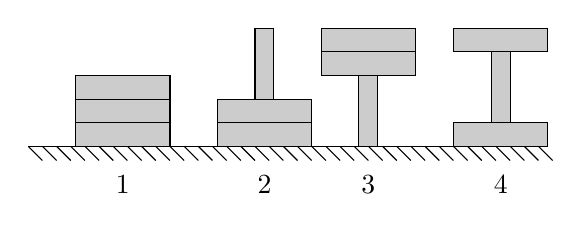
\begin{tikzpicture}[scale=0.6]

% yer (shtrix)
\draw (-1,0) -- (10,0);
\foreach \x in {-1,-0.7,...,10}
{
\draw (\x,0) -- (\x+0.3,-0.3);
}

% --- 1-holat ---
\draw[fill=gray!40] (0,0) rectangle (2,0.5);
\draw[fill=gray!40] (0,0.5) rectangle (2,1);
\draw[fill=gray!40] (0,1) rectangle (2,1.5);
\node at (1,-0.8) {1};

% --- 2-holat ---
\draw[fill=gray!40] (3,0) rectangle (5,0.5);
\draw[fill=gray!40] (3,0.5) rectangle (5,1);
\draw[fill=gray!40] (3.8,1) rectangle (4.2,2.5);
\node at (4,-0.8) {2};

% --- 3-holat ---
\draw[fill=gray!40] (6,0) rectangle (6.4,2);
\draw[fill=gray!40] (5.2,1.5) rectangle (7.2,2);
\draw[fill=gray!40] (5.2,2) rectangle (7.2,2.5);
\node at (6.2,-0.8) {3};

% --- 4-holat ---
\draw[fill=gray!40] (8,0) rectangle (10,0.5);
\draw[fill=gray!40] (8.8,0.5) rectangle (9.2,2);
\draw[fill=gray!40] (8,2) rectangle (10,2.5);
\node at (9,-0.8) {4};

\end{tikzpicture}
\begin{enumerate}[label=\Alph*)]
\item 1
\item 2
\item 3

\item hamma holatlarda bir xil kuch bilan bosadi.
\end{enumerate}



\item G‘isht stol ustiga rasmda tasvirlangandek 3 xil holatda qo‘yilgan. G‘ishtning qaysi holatida uning stolga bosimi eng katta? 

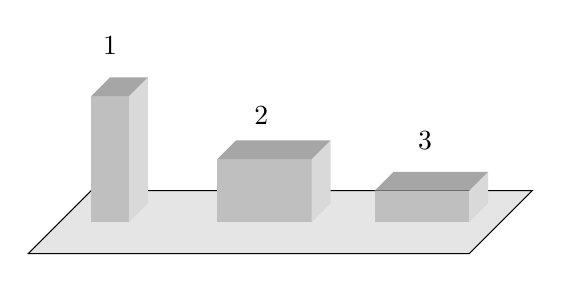
\begin{tikzpicture}[scale=0.8]

% --- platforma (stol) ---

\fill[gray!20] (0,0.2) -- (7,0.2) -- (8,1.2) -- (1,1.2) -- cycle;
\draw (0,0.2) -- (7,0.2) -- (8,1.2) -- (1,1.2) -- cycle;

% --- 1-holat (tik) ---
\fill[gray!50] (1,0.7) rectangle (1.6,2.7);
\fill[gray!30] (1.6,0.7) -- (1.9,1) -- (1.9,3) -- (1.6,2.7) -- cycle;
\fill[gray!70] (1,2.7) -- (1.6,2.7) -- (1.9,3) -- (1.3,3) -- cycle;
\node at (1.3,3.5) {1};

% --- 2-holat (yonboshlab) ---
\fill[gray!50] (3,0.7) rectangle (4.5,1.7);
\fill[gray!30] (4.5,0.7) -- (4.8,1) -- (4.8,2) -- (4.5,1.7) -- cycle;
\fill[gray!70] (3,1.7) -- (4.5,1.7) -- (4.8,2) -- (3.3,2) -- cycle;
\node at (3.7,2.4) {2};

% --- 3-holat (yotgan) ---
\fill[gray!50] (5.5,0.7) rectangle (7,1.2);
\fill[gray!30] (7,0.7) -- (7.3,1) -- (7.3,1.5) -- (7,1.2) -- cycle;
\fill[gray!70] (5.5,1.2) -- (7,1.2) -- (7.3,1.5) -- (5.8,1.5) -- cycle;
\node at (6.3,2) {3};

\end{tikzpicture}

\begin{enumerate}[label=\Alph*)]
\item 1
\item 2
\item 3
\item hamma holatlarda bosim bir xil.

\end{enumerate}

\item Diametri 2 marta ortganda, doira shaklidagi sirtga biror kuchning bosimi qanday 
o‘zgaradi? 
\begin{enumerate}[label=\Alph*)]
\item 2 marta ortadi.
\item 2 marta kamayadi. 
\item 4 marta ortadi.
\item 4 marta kamayadi.
\end{enumerate}

\item Bino bir nechta granit ustunlarga ega bo‘lib, har bir ustunning hajmi 9 m$^3$ ga, asosining yuzi 1,4 m$^2$ ga teng. Granitning zichligi 2800 kg/m$^3$. Bitta ustun o‘z og‘irligi ta’sirida poydevorga qancha bosim (kPa) beradi? 
\begin{enumerate}[label=\Alph*)]
\item 160
\item 200
\item 180
\item 220
\end{enumerate}

\item Blokka osilgan jismlar rasmdagi kabi muvozanatda turibdi. Katta yukning stol sirtiga tegib turgan qismining yuzi 0,4 m$^2$ bo‘lsa, u stolga necha Pa bosim bermoqda? 

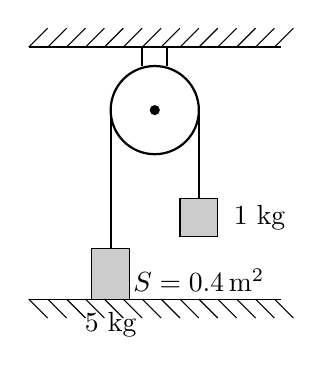
\begin{tikzpicture}[scale=0.8]

% --- shift (tepa) ---
\draw[thick] (-2,4) -- (2,4);
\foreach \x in {-2,-1.7,...,2}
{
\draw (\x,4) -- (\x+0.3,4.3);
}

% --- blok (g‘ildirak) ---
\draw[thick] (0,3) circle (0.7);
\fill (0,3) circle (0.08);

% tayanch
\draw[thick] (-0.2,4) -- (-0.2,3.7);
\draw[thick] (0.2,4) -- (0.2,3.7);

% --- ip ---
\draw[thick] (-0.7,3) -- (-0.7,0.8);
\draw[thick] (0.7,3) -- (0.7,1.6);

% --- chap yuk (5 kg) ---
\draw[fill=gray!40] (-1,0) rectangle (-0.4,0.8);
\node at (-0.7,-0.4) {5 kg};

% stol
\draw (-2,0) -- (2,0);
\foreach \x in {-2,-1.7,...,2}
{
\draw (\x,0) -- (\x+0.3,-0.3);
}

% S yozuvi
\node at (0.7,0.3) {$S=0.4\,\text{m}^2$};

% ipdan yukga
\draw[thick] (-0.7,1) -- (-0.7,1);

% --- o‘ng yuk (1 kg) ---
\draw[fill=gray!40] (0.4,1) rectangle (1,1.6);
\node[right] at (1.1,1.3) {1 kg};

\draw[thick] (0.7,1.2) -- (0.7,1.2);

\end{tikzpicture}
\begin{enumerate}[label=\Alph*)]
\item 100
\item 400
\item 200
\item 500
\end{enumerate}

\item $F=120$ N kuch $S=0,6$ m$^2$ yuzaga vertikalga nisbatan $\alpha=37^\circ$ burchak ostida ta’sir qilmoqda. Bu kuchning bosimini aniqlang (Pa). 

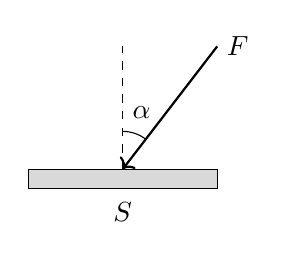
\begin{tikzpicture}[scale=0.6]

% --- sirt (S) ---
\draw[fill=gray!30] (-2,0) rectangle (2,0.4);
\node at (0,-0.5) {$S$};

% --- vertikal (punktir) ---
\draw[dashed] (0,0.4) -- (0,3);

% --- kuch F ---
\draw[<-,thick] (0,0.4) -- (2,3);
\node[right] at (2,3) {$F$};

% --- burchak alpha ---
\draw (0,1.2) arc (90:52:0.8);
\node at (0.4,1.6) {$\alpha$};

\end{tikzpicture}

\begin{enumerate}[label=\Alph*)]
\item 120
\item 300
\item 240
\item 160
\end{enumerate}

\item Qirrasining uzunligi 2 m bo‘lgan kub shaklidagi og`irligi 20 N bo`lib u qiya tekislik ustida tinch turibdi. Jismning qiya tekislik yuzasiga berayotgan bosimini aniqlang (Pa). 

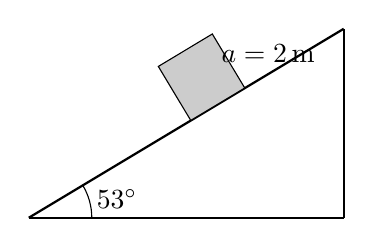
\begin{tikzpicture}[scale=0.8]

% --- qiya tekislik ---
\draw[thick] (0,0) -- (5,0);        % asos
\draw[thick] (0,0) -- (5,3);        % qiya tomon
\draw[thick] (5,0) -- (5,3);        % tik tomon

% --- blok ---
\begin{scope}[rotate=31] % ~53° ga mos vizual
\draw[fill=gray!40] (3,0) rectangle (4,1);
\end{scope}

% --- burchak (53°) ---
\draw (1,0) arc (-180:-149:-1);
\node at (1.4,0.3) {$53^\circ$};

% --- uzunlik yozuvi ---
\node at (3.8,2.6) {$a=2\,\text{m}$};

\end{tikzpicture}

\begin{enumerate}[label=\Alph*)]
\item 5
\item 4
\item 3
\item 2
\end{enumerate}

\item Paskal qonunining to‘g‘ri ta’rifini ko‘rsating. 
\begin{enumerate}[label=\Alph*)]
\item Suyuqlik yoki gazlarga ko‘rsatilgan tashqi bosim ularning hamma nuqtalariga o‘zgarishsiz uzatiladi. 
\item Muvozanatdagi barcha jismlarga berilgan tashqi bosim hamma tomonga bir xil uzatiladi.
\item Suyuqlikka botirilgan jism o‘z og‘irligini qisman yo‘qotadi. 
\item Atmosfera og‘irligi tufayli yerga bosim bilan ta’sir etadi. 

\end{enumerate}

\item Berk idishdagi suyuqliklar va gazlar o‘zlariga berilgan tashqi bosimni ... 
\begin{enumerate}[label=\Alph*)]
\item shu bosim yo‘nalishi bo‘yicha uzatadi. 
\item hamma yo‘nalishlarda bir xil uzatadi. 
\item shu bosimga tik yo‘nalish bo‘yicha uzatadi. 
\item ta’sir etuvchi kuchga qarama-qarshi yo‘nalishda uzatadi. 
\end{enumerate}


\item ... ko‘rsatilgan tashqi bosim barcha yo‘nalishlarda bir xil uzatiladi. 
\begin{enumerate}[label=\Alph*)]
\item faqat suyuqliklarda.
\item faqat gazlarda. 
\item gazlar va suyuqliklarda.
\item qattiq jismlarda. 
\end{enumerate}

\item Ichiga havo qamalgan koptokni siqsak, bosim qayerda ko‘proq ortadi? 
\begin{enumerate}[label=\Alph*)]
\item kuch yo‘nalishida.
\item barcha nuqtasida.
\item pastki qismida.
\item yuqori qismida.

\end{enumerate}
\end{enumerate}





\begin{table}[h!]
\centering
\begin{tabular}{|c|c|c|c|c|c|c|}
\hline
№ & J. & № & J. & № & J.  \\ \hline
1 & C & 6 & D & 11 & A \\ \hline
2 & D & 7 & C & 12 & B \\ \hline
3 & C & 8 & A & 13 & C \\ \hline
4 & C & 9 & D & 14 & B  \\ \hline
5 & A & 10 & A & 15 &   \\ \hline
\end{tabular}
\end{table}
% ...
% \section{Termodinamikaning ikkinchi qonuni. Issiqlik mashinalari}



\begin{enumerate}

\item Issiqlik mashinasining ishchi jismi bo‘lgan gaz ichki energiyasining bir sikl davomidagi o‘zgarishini toping. Sikl davomida gaz isitkichdan $Q_1$ issiqlik miqdori oladi, sovitkichga $Q_2$ issiqlik miqdori beradi va $A$ ish bajaradi.
\begin{enumerate}[label=\Alph*)]
\item $Q_1 - Q_2 + A$
\item $Q_1 - Q_2$
\item $A - Q_1 - Q_2$
\item 0
\end{enumerate}

\item Real issiqlik mashinasi FIK ifodasini ko‘rsating.
\begin{enumerate}[label=\Alph*)]
\item $\frac{Q_1 - Q_2}{Q_2} \cdot 100\%$
\item $\frac{Q_1 - Q_2}{Q_1} \cdot 100\%$
\item $\frac{Q_2 - Q_1}{Q_1} \cdot 100\%$
\item $\frac{T_1 - T_2}{T_1} \cdot 100\%$
\end{enumerate}

\item Real issiqlik mashinasida ishchi qism isitkichdan 2 kJ issiqlik olib, sovitkichga 600 J issiqlik berdi. Uning bajargan foydali ishini toping (J).
\begin{enumerate}[label=\Alph*)]
\item 2600
\item 2000
\item 1400
\item 600
\end{enumerate}

\item Real issiqlik mashinasida ishchi qism isitkichdan 600 J issiqlik olib, 400 J foydali ish bajardi. U sovitkichga qancha issiqlik bergan (J)?
\begin{enumerate}[label=\Alph*)]
\item 1000
\item 2000
\item 0
\item 600
\end{enumerate}

\item Real issiqlik mashinasi 520 J foydali ish bajardi. Bunda sovitkichga 180 J issiqlik berildi. Ishchi qism isitkichdan qancha issiqlik olgan (J)?
\begin{enumerate}[label=\Alph*)]
\item 700
\item 0
\item 180
\item 520
\end{enumerate}

\item Issiqlik mashinasi sikl davomida isitkichdan 100 J issiqlik oldi va sovitkichga 60 J issiqlik berdi. Mashinaning FIK ni toping.
\begin{enumerate}[label=\Alph*)]
\item 67\%
\item 60\%
\item 40\%
\item 25\%
\end{enumerate}

\item FIK $\eta$ bo‘lgan issiqlik mashinasi isitkichdan $Q$ issiqlik miqdori olganda qanday ish bajaradi?
\begin{enumerate}[label=\Alph*)]
\item $\eta Q$
\item $(1 + \eta)Q$
\item $(1 - \eta)Q$
\item $Q / \eta$
\end{enumerate}

\item Issiqlik dvigateli isitkichdan har sekundda 7200 kJ issiqlik oladi va sovitkichga 6400 kJ issiqlik beradi. Dvigatelning FIK qanday?
\begin{enumerate}[label=\Alph*)]
\item 62\%
\item 41\%
\item 24\%
\item 11\%
\end{enumerate}

\item Issiqlik dvigateli isitkichdan 0,8 MJ issiqlik miqdori olib, sovitkichga 0,3 MJ issiqlik miqdorini beradi. Bu issiqlik dvigatelining FIK ni (\%) toping.
\begin{enumerate}[label=\Alph*)]
\item 30
\item 48
\item 50
\item 62,5
\end{enumerate}

\item Issiqlik dvigateli isitkichdan 0,4 MJ issiqlik miqdori olib, sovitkichga 0,26 MJ issiqlik miqdorini uzatadi. Dvigatelning FIK ni hisoblang (\%).
\begin{enumerate}[label=\Alph*)]
\item 30
\item 35
\item 40
\item 45
\end{enumerate}

\item Bitta siklda issiqlik mashinasi 28 kJ ish bajarib, sovitkichga 42 kJ issiqlik miqdorini beradi. Mashinaning FIK ni aniqlang (\%).
\begin{enumerate}[label=\Alph*)]
\item 30
\item 42
\item 40
\item 50
\end{enumerate}

\item FIK 25\% bo‘lgan issiqlik mashinasi sovitkichga 600 J issiqlik beradi. U qanday foydali ish bajaradi (J)?
\begin{enumerate}[label=\Alph*)]
\item 200
\item 300
\item 400
\item 500
\end{enumerate}

\item FIK 40\% bo‘lgan issiqlik mashinasi bitta siklda sovitkichga 42 kJ issiqlik beradi. Mashina bitta siklda necha kJ ish bajaradi?
\begin{enumerate}[label=\Alph*)]
\item 21
\item 28
\item 168
\item 56
\end{enumerate}

\item Issiqlik mashinasining FIK 25\%. Uning isitkichdan olgan issiqlik miqdori 800 J bo‘lsa, foydali ishi necha Joul bo‘ladi?
\begin{enumerate}[label=\Alph*)]
\item 100
\item 200
\item 300
\item 400
\end{enumerate}

\item Foydali ish koeffitsienti 30\% bo‘lgan ideal issiqlik mashinasi qizdirgichdan 10 kJ issiqlik oladi. Sovitkichga berilayotgan issiqlik miqdori qanday (kJ)?
\begin{enumerate}[label=\Alph*)]
\item 6
\item 7
\item 3
\item 2,4
\end{enumerate}

\item Isitkichning harorati $150^\circ C$, sovitkichniki $20^\circ C$. Ideal issiqlik mashinasining FIK necha foiz?
\begin{enumerate}[label=\Alph*)]
\item 20
\item 23
\item 25
\item 30,7
\end{enumerate}

\item Ideal issiqlik mashina isitkichining harorati $117^\circ C$, sovitkichniki $27^\circ C$. Mashinaning FIK ni toping (\%).
\begin{enumerate}[label=\Alph*)]
\item 23
\item 33
\item 70
\item 30
\end{enumerate}

\item Karno siklida ishlayotgan issiqlik mashinasiga temperaturasi $480^\circ C$ bo‘lgan bug‘ kirib, undan $30^\circ C$ temperaturada chiqsa, mashinaning FIK qanday (\%)?
\begin{enumerate}[label=\Alph*)]
\item 30
\item 40
\item 50
\item 60
\end{enumerate}

\item Bug‘ turbinasiga bug‘ $500^\circ C$ harorat bilan kirib, undan $30^\circ C$ harorat bilan chiqib ketadi. Bug‘ turbinasini ideal issiqlik mashinasi deb hisoblab, uning FIK ni toping (\%).
\begin{enumerate}[label=\Alph*)]
\item 30
\item 47
\item 61
\item 77
\end{enumerate}

\item Isitkichining harorati $227^\circ C$, sovitkichniki $27^\circ C$ bo‘lgan issiqlik mashinasining maksimal FIK necha foiz?
\begin{enumerate}[label=\Alph*)]
\item 20
\item 30
\item 40
\item 45
\end{enumerate}

\item FIK ning maksimal qiymati 50\% bo‘lishi uchun isitkichining harorati $527^\circ C$ bo‘lgan issiqlik mashinasi sovitkichining harorati qanday ($^\circ C$) bo‘lishi kerak?
\begin{enumerate}[label=\Alph*)]
\item 400
\item 351
\item 263,5
\item 127
\end{enumerate}

\item Isitkichining harorati 500 K bo‘lgan issiqlik mashinasining FIK 50\%. Sovitkichning harorati qanday (K)?
\begin{enumerate}[label=\Alph*)]
\item 190
\item 200
\item 230
\item 250
\end{enumerate}

\item FIK ning maksimal qiymati 70\% bo‘lishi uchun isitkichining harorati $727^\circ C$ bo‘lgan issiqlik mashinasi sovitkichining harorati qanday ($^\circ C$) bo‘lishi kerak?
\begin{enumerate}[label=\Alph*)]
\item 27
\item 218
\item 300
\item 315
\end{enumerate}

\item Isitkich harorati $427^\circ C$ bo‘lib, sovitkich harorati $127^\circ C$. Issiqlik mashinasi bir siklda 600 J issiqlik olib, sovitkichga 400 J issiqlik beradi. Real mashinaning FIK ideal mashina FIK ning qancha qismini tashkil qiladi?
\begin{enumerate}[label=\Alph*)]
\item 1/2
\item 6/7
\item 7/8
\item 7/9
\end{enumerate}

\item FIK $\eta$ bo‘lgan issiqlik dvigatelida gaz bajargan ishni 13 marta oshirish uchun isitkichdan olinadigan issiqlik miqdorini qanday o‘zgartirish kerak? $\eta = const$.
\begin{enumerate}[label=\Alph*)]
\item $13/\eta$ marta orttirish
\item 13 marta orttirish
\item 13 marta kamaytirish
\item $13\eta$ marta orttirish
\end{enumerate}

\item Karno siklida ishlaydigan mashinada isitkich va sovitkich absolyut temperaturalarining nisbati 5 ga teng. Agar bir siklda sovitkichga 36 kJ issiqlik berilgan bo‘lsa, isitkichdan olingan issiqlik miqdori qanday (kJ)?
\begin{enumerate}[label=\Alph*)]
\item 900
\item 180
\item 72
\item 7,2
\end{enumerate}

\item Ideal issiqlik mashinasi bir sikl davomida $5,36 \cdot 10^4$ J ish bajardi. Isitkich temperaturasi $100^\circ C$, sovitkichniki esa $0^\circ C$ bo‘lsa, mashina bir siklda isitkichdan qanday (kJ) issiqlik miqdori oladi?
\begin{enumerate}[label=\Alph*)]
\item 150
\item 170
\item 200
\item 210
\end{enumerate}

\item Isitkichining temperaturasi $T_1$, sovitkichining temperaturasi $T_2$ bo‘lgan issiqlik mashinasi bor. $T_1$ ni $\Delta T$ ga orttirib, $T_2$ ni o‘zgartirmagan va $T_2$ ni $\Delta T$ ga kamaytirib, $T_1$ ni o‘zgartirmagan hollardagi FIK larning nisbatini toping.
\begin{enumerate}[label=\Alph*)]
\item $\frac{T_1 - \Delta T}{T_1}$
\item $\frac{T_1 + \Delta T}{T_2 + \Delta T}$
\item $\frac{T_1}{T_1 + \Delta T}$
\item $\frac{T_1 - T_2}{T_1}$
\end{enumerate}

\item Rasmda ko‘rsatilgan siklning qaysi qismida gaz manfiy ish bajaradi?

\begin{tikzpicture}[>=stealth, scale=1]
    % Koordinata o'qlari
    \draw[->, thick] (0,0) -- (4,0) node[right] {$T$};
    \draw[->, thick] (0,0) -- (0,3.5) node[above] {$P$};
    \node[below left] at (0,0) {$O$};

    % Nuqtalarni belgilash
    \coordinate (1) at (1.5, 1.2);
    \coordinate (2) at (1.5, 2.5);
    \coordinate (3) at (3, 2.5);

    % 1-2 jarayon (Izotermik siqilish - T=const, P ortmoqda)
    \draw[thick, ->] (1) -- (2);
    \node[left] at (1) {1};
    \node[left] at (2) {2};

    % 2-3 jarayon (Izobarik kengayish - P=const, T ortmoqda)
    \draw[thick, ->] (2) -- (3);
    \node[above] at (3) {3};

    % 3-1 jarayon (Izoxorik sovish - V=const, chiziq koordinata boshiga yo'nalgan)
    \draw[thick, ->] (3) -- (1);
    \draw[dashed] (0,0) -- (1);

\end{tikzpicture}

\begin{enumerate}[label=\Alph*)]
\item bunda gaz manfiy ish bajarmaydi
\item 2-3
\item 1-2
\item 3-1
\end{enumerate}

\item Gazning rasmda ko‘rsatilgan siklni o‘tishda bajargan ishini toping.

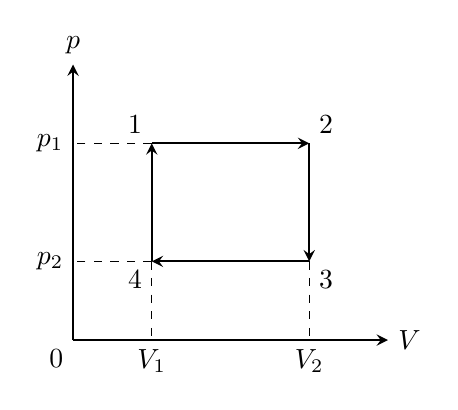
\begin{tikzpicture}[>=stealth, scale=1]
    % Koordinata o'qlari
    \draw[->, thick] (0,0) -- (4,0) node[right] {$V$};
    \draw[->, thick] (0,0) -- (0,3.5) node[above] {$p$};
    \node[below left] at (0,0) {0};

    % Nuqtalar koordinatalari
    \coordinate (1) at (1, 2.5);
    \coordinate (2) at (3, 2.5);
    \coordinate (3) at (3, 1);
    \coordinate (4) at (1, 1);

    % Sikl chizig'i va yo'nalish strelkalari
    \draw[thick, ->] (1) -- (2);
    \draw[thick, ->] (2) -- (3);
    \draw[thick, ->] (3) -- (4);
    \draw[thick, ->] (4) -- (1);

    % Nuqta raqamlari
    \node[above left] at (1) {1};
    \node[above right] at (2) {2};
    \node[below right] at (3) {3};
    \node[below left] at (4) {4};

    % O'qlardagi proyeksiyalar va labellar
    \draw[dashed] (1) -- (0, 2.5) node[left] {$p_1$};
    \draw[dashed] (4) -- (0, 1) node[left] {$p_2$};
    \draw[dashed] (4) -- (1, 0) node[below] {$V_1$};
    \draw[dashed] (3) -- (3, 0) node[below] {$V_2$};
\end{tikzpicture}

\begin{enumerate}[label=\Alph*)]
\item $(p_1 - p_2)(V_2 - V_1)$
\item $p_2(V_2 - V_1)$
\item $(p_1 - p_2)V_1$
\item $(p_1 - p_2)V_2$
\end{enumerate}

\item Rasmda ko‘rsatilgan siklda bajarilgan ishni quyidagi ifodalarning qaysi biridan foydalanib topish mumkin?

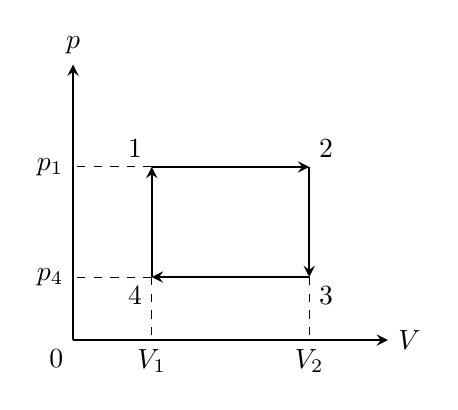
\begin{tikzpicture}[>=stealth, scale=1]
    % Koordinata o'qlari
    \draw[->, thick] (0,0) -- (4,0) node[right] {$V$};
    \draw[->, thick] (0,0) -- (0,3.5) node[above] {$p$};
    \node[below left] at (0,0) {0};

    % Nuqtalar koordinatalari
    \coordinate (A) at (1, 2.2);
    \coordinate (B) at (3, 2.2);
    \coordinate (C) at (3, 0.8);
    \coordinate (D) at (1, 0.8);

    % Sikl chizig'i va yo'nalish strelkalari
    \draw[thick, ->] (A) -- (B);
    \draw[thick, ->] (B) -- (C);
    \draw[thick, ->] (C) -- (D);
    \draw[thick, ->] (D) -- (A);

    % Nuqta raqamlari
    \node[above left] at (A) {1};
    \node[above right] at (B) {2};
    \node[below right] at (C) {3};
    \node[below left] at (D) {4};

    % O'qlardagi proyeksiyalar (formula uchun zaruriy parametrlar)
    \draw[dashed] (A) -- (0, 2.2) node[left] {$p_1$};
    \draw[dashed] (D) -- (0, 0.8) node[left] {$p_4$};
    \draw[dashed] (D) -- (1, 0) node[below] {$V_1$};
    \draw[dashed] (C) -- (3, 0) node[below] {$V_2$};
\end{tikzpicture}

\begin{enumerate}[label=\Alph*)]
\item $(p_1 + p_2)(V_2 - V_1)$
\item $p_2(V_2 - V_1)$
\item $(p_1 - p_4)(V_2 - V_1)$
\item $p_1(V_2 - V_1)$
\end{enumerate}

\item Diagrammada ko‘rsatilgan sikl bo‘yicha ishlovchi issiqlik mashinasi bir sikl davomida qanday (kJ) ish bajaradi?

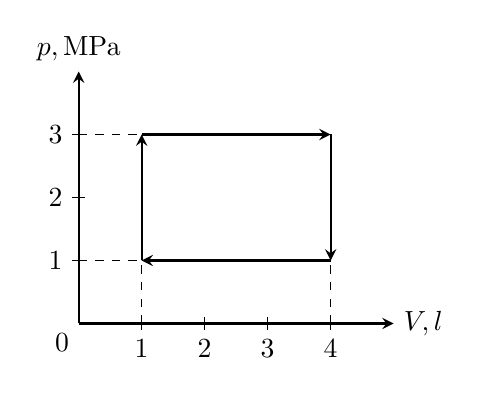
\begin{tikzpicture}[>=stealth, scale=0.8]
    % Koordinata o'qlari
    \draw[->, thick] (0,0) -- (5,0) node[right] {$V, l$};
    \draw[->, thick] (0,0) -- (0,4) node[above] {$p, \text{MPa}$};
    \node[below left] at (0,0) {0};

    % O'qlardagi bo'linmalar (V o'qi)
    \foreach \x in {1,2,3,4}
        \draw (\x, 0.1) -- (\x, -0.1) node[below] {\x};
        
    % O'qlardagi bo'linmalar (p o'qi)
    \foreach \y in {1,2,3}
        \draw (0.1, \y) -- (-0.1, \y) node[left] {\y};

    % Sikl nuqtalari
    \coordinate (A) at (1,1);
    \coordinate (B) at (1,3);
    \coordinate (C) at (4,3);
    \coordinate (D) at (4,1);

    % Sikl chiziqlari va yo'nalish strelkalari (Clockwise)
    \draw[thick, ->] (A) -- (B); % Izoxorik isitish
    \draw[thick, ->] (B) -- (C); % Izobarik kengayish
    \draw[thick, ->] (C) -- (D); % Izoxorik sovutish
    \draw[thick, ->] (D) -- (A); % Izobarik siqilish

    % Proyeksiya chiziqlari (punktir)
    \draw[dashed] (1,0) -- (1,1);
    \draw[dashed] (4,0) -- (4,1);
    \draw[dashed] (0,1) -- (1,1);
    \draw[dashed] (0,3) -- (1,3);

\end{tikzpicture}

\begin{enumerate}[label=\Alph*)]
\item 3
\item 6
\item 8
\item 9
\end{enumerate}

\item Diagrammada ko‘rsatilgan sikl bo‘yicha ishlovchi issiqlik mashinasi bir sikl davomida qanday (kJ) ish bajaradi?

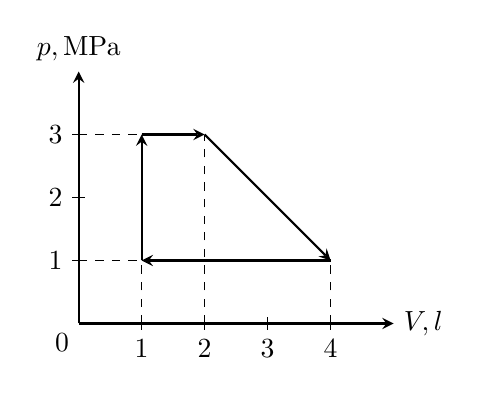
\begin{tikzpicture}[>=stealth, scale=0.8]
    % Koordinata o'qlari
    \draw[->, thick] (0,0) -- (5,0) node[right] {$V, l$};
    \draw[->, thick] (0,0) -- (0,4) node[above] {$p, \text{MPa}$};
    \node[below left] at (0,0) {0};

    % V o'qidagi bo'linmalar
    \foreach \x in {1,2,3,4}
        \draw (\x, 0.1) -- (\x, -0.1) node[below] {\x};
        
    % p o'qidagi bo'linmalar
    \foreach \y in {1,2,3}
        \draw (0.1, \y) -- (-0.1, \y) node[left] {\y};

    % Sikl nuqtalari koordinatalari
    \coordinate (A) at (1,1);
    \coordinate (B) at (1,3);
    \coordinate (C) at (2,3);
    \coordinate (D) at (4,1);

    % Sikl chiziqlari va yo'nalish strelkalari
    \draw[thick, ->] (A) -- (B); % Izoxorik isitish (1 -> 3 MPa)
    \draw[thick, ->] (B) -- (C); % Izobarik kengayish (1 -> 2 l)
    \draw[thick, ->] (C) -- (D); % O'zgaruvchan jarayon (diagonall)
    \draw[thick, ->] (D) -- (A); % Izobarik siqilish (4 -> 1 l)

    % Proyeksiya (punktir) chiziqlari
    \draw[dashed] (1,0) -- (1,1);
    \draw[dashed] (2,0) -- (2,3);
    \draw[dashed] (4,0) -- (4,1);
    \draw[dashed] (0,1) -- (1,1);
    \draw[dashed] (0,3) -- (1,3);

\end{tikzpicture}

\begin{enumerate}[label=\Alph*)]
\item 3
\item 4
\item 6
\item 7
\end{enumerate}

\end{enumerate}



\begin{table}[h!]
\centering
\begin{tabular}{|c|c|c|c|c|c|c|c|c|c|}
\hline
№ & J. & № & J. & № & J. & № & J. & № & J. \\ \hline
1 & D & 8 & D & 15 & B & 22 & D & 29 & C \\ \hline
2 & B & 9 & D & 16 & D & 23 & A & 30 & A \\ \hline
3 & C & 10 & B & 17 & A & 24 & D & 31 & C \\ \hline
4 & B & 11 & C & 18 & D & 25 & B & 32 & B \\ \hline
5 & A & 12 & A & 19 & C & 26 & B & 33 & B \\ \hline
6 & C & 13 & B & 20 & C & 27 & C & & \\ \hline
7 & A & 14 & B & 21 & D & 28 & C & & \\ \hline
\end{tabular}
\end{table}


% ==================================================
%                    ELEKTR VA MAGNITIZM
% ==================================================

% \newpage
% \part{ELEKTR VA MAGNITIZM}

% \section{Elektr zaryadlari. Kulon qonuni}



\begin{enumerate}

\item Vakuumda joylashgan nuqtaviy musbat $q_1$ zaryadning o'zidan $r$ masofada joylashgan nuqtaviy musbat $q_2$ zaryadga ko'rsatadigan ta'sir kuchi ifodasini ko'rsating.
\begin{enumerate}[label=\Alph*)]
\item $F = \frac{1}{4\pi\epsilon_0} \frac{q_1 q_2}{r^2}$
\item $F = -k \frac{q_1 q_2}{r^3}$
\item $F = \frac{1}{4\pi\epsilon_0} \frac{q_1 q_2}{r^3}$
\item $F = \frac{1}{4\pi\epsilon_0 \epsilon} \frac{q_1 q_2}{r}$
\end{enumerate}

\item Ikki sharchaga bir xil $2 \cdot 10^{-8} \, C$ zaryad berilgan. Zaryadlar bir-birini $5 \cdot 10^{-4} \, N$ kuch bilan itarishmoqda. Sharchalar orasidagi masofa (sm) qancha?
\begin{enumerate}[label=\Alph*)]
\item 7,5
\item 8,5
\item 8
\item 7
\end{enumerate}

\item Ikkita bir xil sharcha bir-biridan 10 sm masofada turibdi. Ular bir xil miqdorda manfiy zaryadga ega bo'lib, 0,23 mN kuch bilan o'zaro ta'sirlashadi. Har qaysi sharchadagi "ortiqcha" elektronlar sonini toping.
\begin{enumerate}[label=\Alph*)]
\item $1,0 \cdot 10^8$
\item $1,0 \cdot 10^{11}$
\item $1,0 \cdot 10^{14}$
\item $1,0 \cdot 10^{12}$
\end{enumerate}

\item Nuqtaviy zaryadlarning o'zaro ta'sir kuchi 10 mN, zaryad miqdorlari $5,2 \cdot 10^{-6} \, C$ va $5 \cdot 10^{-6} \, C$ bo'lsa, ular orasidagi masofa (m) qanday?
\begin{enumerate}[label=\Alph*)]
\item 10,15
\item 0,31
\item 1
\item 4,83
\end{enumerate}

\item 6,6 mKl va 11 mKl zaryadlar suvda bir-biridan 3,3 sm masofada turib, qanday kuch bilan o'zaro ta'sirlashadi?
\begin{enumerate}[label=\Alph*)]
\item $18 \cdot 10^{-2}$
\item $7,8 \cdot 10^{-2}$
\item $6,4 \cdot 10^{-4}$
\item TJY
\end{enumerate}

\item Bir-biridan 30 sm (markazlari orasidagi) masofada turgan ikkita birday zaryadlangan sharcha o'zaro 10 dina kuch bilan ta'sirlashadi. Sharchalardan biridagi zaryadni toping (pC)? $1 Dina = 10^{-10} \, N$.
\begin{enumerate}[label=\Alph*)]
\item 484
\item 424
\item 252
\item 100
\end{enumerate}

\item Nuqtaviy zaryadlar orasidagi masofa 3 marta o'zgartirilsa, ularning o'zaro ta'sir kuchi necha marta o'zgaradi?
\begin{enumerate}[label=\Alph*)]
\item 3
\item 9
\item 27
\item 81
\end{enumerate}

\item Agar ikki nuqtaviy zaryadning zaryadi to'rt baravar orttirilsa, ular orasidagi masofa esa ikki marta kamaytirilsa, ular orasidagi o'zaro ta'sir kuchi qanday o'zgaradi?
\begin{enumerate}[label=\Alph*)]
\item 8 marta kamayadi
\item 8 marta ortadi
\item 64 marta ortadi
\item 2 marta kamayadi
\end{enumerate}

\item Ikki nuqtaviy zaryad orasidagi masofa 3 marta ortsa, ular orasidagi ta'sir kuchi qanday o'zgaradi?
\begin{enumerate}[label=\Alph*)]
\item 3 marta oshadi
\item 9 marta kamayadi
\item o'zgarmaydi
\item 3 marta kamayadi
\end{enumerate}

\item Vakuumda joylashgan ikkita zaryadlangan zarracha o'zaro ta'sirlashmoqda. Agar zaryadlardan birini ikki marta orttirib, boshqa zaryad 4 marta kamaytirilsa hamda ularning orasidagi masofa 3 marta kamaytirilsa, ular orasidagi Kulon kuchi qanday o'zgaradi?
\begin{enumerate}[label=\Alph*)]
\item 6 marta kamayadi
\item 4,5 marta ortadi
\item 2,5 marta ortadi
\item 9 marta ortadi
\end{enumerate}

\item Radiusi 5 sm bo'lgan va $q = +15 \, nC$ zaryadga ega bo'lgan mis halqa o'z markazida joylashgan $q_1 = -3 \, nC$ nuqtaviy zaryadga qanday kuch bilan ta'sir qiladi?
\begin{enumerate}[label=\Alph*)]
\item 0
\item 40
\item 80
\item 160
\end{enumerate}

\item Havoda 3 sm masofada turgan ikki zaryad bir-biri bilan $2 \cdot 10^{-5} \, N$ kuch orqali ta'sirlashadi. Qandaydir suyuq muhitda shu zaryadlar 5 sm masofadan turib, $1,5 \cdot 10^{-6} \, N$ kuch bilan ta'sirlashadi. Shu suyuq muhitning dielektrik singdiruvchanligini aniqlang.
\begin{enumerate}[label=\Alph*)]
\item $\approx 12$
\item $\approx 5$
\item $\approx 0,2$
\item $\approx 1$
\end{enumerate}

\item Ikkita zaryad suvda bir-biriga 3 sm masofada qanday kuch bilan o'zaro ta'sirlashsa, vakuumda 27 sm masofada ham shunday kuch bilan o'zaro ta'sirlashadi. Suvning dielektrik singdiruvchanligi qancha?
\begin{enumerate}[label=\Alph*)]
\item 81
\item 98
\item 76
\item 9
\end{enumerate}

\item Ikkita zaryad vakuumda $r_1$ masofadan o'zaro ta'sirlashdi. Ularning o'zaro ta'sir kuchini o'zgartirmasdan singdiruvchanligi $\epsilon$ bo'lgan dielektrikda qanday $r_2$ masofada joylashtirish kerak?
\begin{enumerate}[label=\Alph*)]
\item $r_2 = \sqrt{r_1 \epsilon}$
\item $r_2 = \frac{\sqrt{\epsilon}}{r_1}$
\item $r_2 = \frac{r_1}{\sqrt{\epsilon}}$
\item $r_2 = r_1 \sqrt{\epsilon}$
\end{enumerate}

\item Ikkita zaryad havoda bir-biridan $r_1$ masofada turibdi. Ular orasidagi ta'sir kuchi o'zgarmasdan qolishi uchun ularni dielektrik singdiruvchanligi $\epsilon_2$ bo'lgan boshqa muhitda qanday $r_2$ masofada joylashtirish kerak?
\begin{enumerate}[label=\Alph*)]
\item $r_1 = r_2 \sqrt{\epsilon_2}$
\item $r_2 = r_1 \sqrt{\epsilon_2}$
\item $r_2 = 2r_1 \sqrt{\epsilon_2}$
\item $r_1 = r_2 \epsilon_2$
\end{enumerate}

\item $q_1 = q$ va $q_2 = 3q$ zaryadli ikkita bir xil metal sharcha bir-biriga tekkizildi va avvalgi joyiga qaytarildi. Bunda ularning o'zaro ta'sir kuchi necha marta ortadi?
\begin{enumerate}[label=\Alph*)]
\item 9/8
\item 4/3
\item 9/5
\item 9/4
\end{enumerate}

\item $3q$ va $5q$ zaryadli ikkita bir xil metall sharcha bir-biriga tekkizildi va avvalgi vaziyatiga qaytarildi. Bunda ularning o'zaro ta'sir kuchi necha marta ortadi?
\begin{enumerate}[label=\Alph*)]
\item 49/48
\item 16/15
\item 25/21
\item 121/96
\end{enumerate}

\item Biriga N ta, ikkinchisiga N-1 ta elektron yetishmayotgan ikkita bir xil sharcha bir-biridan d masofada turib $F_1$ kuch bilan ta'sirlashyapti. Ular bir-biriga tekkizilib yana oldingi vaziyatiga qaytganda $F_2$ kuch bilan ta'sirlashadi. $F_1/F_2$ nisbat nimaga teng? $N \ge 2$.
\begin{enumerate}[label=\Alph*)]
\item 1
\item $\frac{N(4N-1)}{(2N-1)^2}$
\item $\frac{4N(N-1)}{(2N-1)^2}$
\item $\frac{4N(2N-1)}{(N-1)^2}$
\end{enumerate}

\item Bir xil ishorali $q$ va $4q$ zaryadlar bilan zaryadlangan ikkita bir xil metall sharcha bir-biridan r masofada turibdi. Sharchalar bir-biriga tekkiziladi. O'zaro ta'sir kuchi avvalgidek qolishi uchun ularni qanday masofaga surish lozim?
\begin{enumerate}[label=\Alph*)]
\item 2,5r
\item 0,4r
\item r
\item 1,25r
\end{enumerate}

\item Oralaridagi masofa diametrlaridan juda kichik bo'lgan ikki yassi metall plastina qarama-qarshi ishorali, kattaligi bir xil bo'lgan zaryadlar bilan zaryadlangan va bir-biriga F kuch bilan tortiladi. Agar plastinalar orasidagi masofa 2 marta orttirilsa, bu kuch qanday o'zgaradi?
\begin{enumerate}[label=\Alph*)]
\item 4 marta kamayadi
\item 2 marta kamayadi
\item deyarli o'zgarmaydi
\item $\sqrt{2}$ marta kamayadi
\end{enumerate}

\item Quyidagilarni qaysi biri elektr doimiysini birligi hisoblanadi?
\begin{enumerate}[label=\Alph*)]
\item $kg \cdot m^{-3} \cdot s^{-4} \cdot A^2$
\item $kg \cdot m^2 \cdot s^{-3} \cdot A^3$
\item $kg^{-2} \cdot m^2 \cdot s^3 \cdot A^2$
\item $kg^{-1} \cdot m^{-3} \cdot s^4 \cdot A^2$
\end{enumerate}

\item Ikkita bir xil nuqtaviy $q$ zaryadlar o'rtasiga $q/2$ zaryad joylashtirilsa, $q$ zaryadga ta'sir qiluvchi kuch necha marta ortadi?
\begin{enumerate}[label=\Alph*)]
\item 1,5
\item 2
\item 3
\item 4
\end{enumerate}

\item Uzunligi 100 sm li iplarga osilgan, har birining massasi 0,25 g bo'lgan $q_1 = q_2$ zaryadli ikkita sharcha bir-biridan 6 sm qochgan. Har bir sharchaning zaryadi necha nKl ga teng?
\begin{enumerate}[label=\Alph*)]
\item 5,4
\item 6,7
\item 7,9
\item 10
\end{enumerate}

\item Chizmadagi zaryadlangan sharchalarning o'zaro ta'sir kuchi necha nyuton ekanligini aniqlang? Ulardan biri qo'zg'almas ($g = 10 \, m/s^2, m = 10 \, g, \tan 35^\circ = 0,7$).


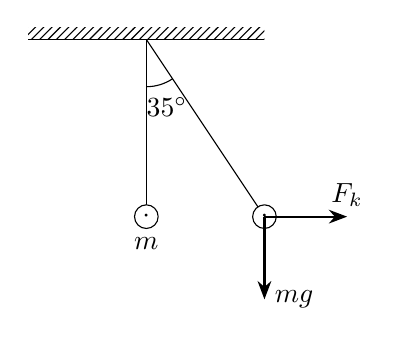
\begin{tikzpicture}[scale=1.5, >=Stealth]
    % Ship (Ceiling)
    \fill[pattern=north east lines] (-1,2) rectangle (1,2.1);
    \draw (-1,2) -- (1,2);
    
    % Vertikal osilgan sharcha
    \draw (0,2) -- (0,0.5);
    \draw[fill=white] (0,0.5) circle (0.1) node[below=4pt] {$m$};
    \node at (0,0.5) {$\cdot$};
    
    % Burchak ostidagi sharcha
    \draw (0,2) -- (1,0.5);
    \draw[fill=white] (1,0.5) circle (0.1);
    \node at (1,0.5) {$\cdot$};
    
    % Kuchlar (mg va F_k)
    \draw[->, thick] (1,0.5) -- (1,-0.2) node[right] {$mg$};
    \draw[->, thick] (1,0.5) -- (1.7,0.5) node[above] {$F_k$};
    
    % Burchak 35 gradus
    \draw[dashed] (0,2) -- (0,1);
    \coordinate (top) at (0,2);
    \coordinate (vert) at (0,1);
    \coordinate (side) at (1,0.5);
    \pic [draw, "35$^\circ$", angle eccentricity=1.5, angle radius=0.6cm] {angle = vert--top--side};
\end{tikzpicture}
\begin{enumerate}[label=\Alph*)]
\item 0,07
\item 0,7
\item 7
\item 10
\end{enumerate}

\item Radiusi $5 \, sm$ bo'lgan aylanaga zaryadining moduli $q = 2 \, \mu C$ bo'lgan 3 ta zaryad va markazga zaryadining moduli $Q = 5 \, \mu C$ bo'lgan boshqa zaryad joylashtirildi. Aylananing markazidagi zaryadga ta'sir qiladigan natijaviy Kulon kuchini toping ($\mu N$). ($\alpha = 60^\circ$).

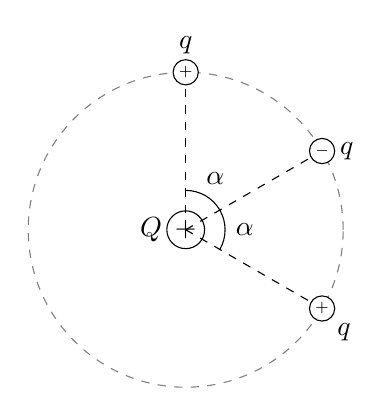
\begin{tikzpicture}[scale=2, >=stealth]
    % Aylana (punktir chiziq bilan)
    \draw[dashed, color=gray] (0,0) circle (1);

    % Markazdagi zaryad (Q+)
    \draw[fill=white] (0,0) circle (0.12) node {$+$};
    \node[left=5pt] at (0,0) {$Q$};

    % Zaryadlarning o'rni (alfa = 60 gradus bo'lganda: 90, 30, -30 graduslar)
    
    % 1. Yuqoridagi musbat zaryad (90 gradusda)
    \draw[dashed] (0,0) -- (90:1);
    \draw[fill=white] (90:1) circle (0.08) node {\tiny $+$};
    \node[above=3pt] at (90:1) {$q$};

    % 2. O'rtadagi manfiy zaryad (30 gradusda)
    \draw[dashed] (0,0) -- (30:1);
    \draw[fill=white] (30:1) circle (0.08) node {\tiny $-$};
    \node[right=3pt] at (30:1) {$q$};

    % 3. Pastdagi musbat zaryad (-30 gradusda)
    \draw[dashed] (0,0) -- (-30:1);
    \draw[fill=white] (-30:1) circle (0.08) node {\tiny $+$};
    \node[below right=2pt] at (-30:1) {$q$};

    % Burchaklarni belgilash (alfa)
    \coordinate (O) at (0,0);
    \coordinate (T) at (90:0.7);
    \coordinate (M) at (30:0.7);
    \coordinate (B) at (-30:0.7);

    \pic [draw, "$\alpha$", angle eccentricity=1.5, angle radius=0.5cm] {angle = M--O--T};
    \pic [draw, "$\alpha$", angle eccentricity=1.5, angle radius=0.5cm] {angle = B--O--M};

\end{tikzpicture}

\begin{enumerate}[label=\Alph*)]
\item 22
\item 32
\item 0
\item 54
\end{enumerate}
\end{enumerate}

\begin{table}[h!]
\centering
\begin{tabular}{|c|c|c|c|c|c|c|c|c|c|}
\hline
№ & J. & № & J. & № & J. & № & J. & № & J. \\ \hline
1 & A & 6 & D & 11 & A & 16 & B & 21 & D \\ \hline
2 & B & 7 & B & 12 & B & 17 & B & 22 & C \\ \hline
3 & B & 8 & C & 13 & A & 18 & C & 23 & B \\ \hline
4 & D & 9 & B & 14 & C & 19 & D & 24 & A\\ \hline
5 & D & 10 & B & 15 & A & 20 & C & 25 &C \\ \hline
\end{tabular}
\end{table}

\section{Elektr maydon. Elektr maydon kuchlanganligi}


\begin{enumerate}

    \item Zaryadlangan zarracha vakuumning qandaydir nuqtasida 60 V/m kuchlanganlik hosil qiladi. Agar butun sistema dielektrik singdiruvchanligi 2 bo’lgan kerosin ichiga joylashtirilsa, shu nuqtaga o’rnatilgan 5 nC zaryadga qanday kuch (nN da) ta’sir qiladi? 
    \begin{enumerate}[label=\Alph*)]
        \item 300
        \item 150 % To'g'ri
        \item 75
        \item 60
    \end{enumerate}

    \item Kuchlanganlik vektori vertikal yuqoriga yo’nalgan bir jinsli elektr maydonda massasi 0,03 mkg bo’lgan 3 pC zaryadli chang zarrachasi muvozanat holatida turibdi. Maydon kuchlanganligini aniqlang ($g=10 \, m/s^2$). 
    \begin{enumerate}[label=\Alph*)]
        \item 100 % To'g'ri
        \item 10
        \item 1000
        \item 1
    \end{enumerate}

    \item Miqdori 20 kV/m bo’lgan kuchlanganlik vektori vertikal pastga yo’nalgan bir jinsli elektr maydonda 0,1 kg massali va 0,2 mC zaryadli sharcha ipak ipga osilgan. Ipning taranglik kuchini toping ($g=10 \, m/s^2$). 
    \begin{enumerate}[label=\Alph*)]
        \item 1
        \item 3
        \item 5 % To'g'ri
        \item 10
    \end{enumerate}

    \item Agar ipga osilgan 0,1 kg massadagi 10 mkC zaryadli sharcha 200 kV/m kuchlanganlikka ega bo’lgan bir jinsli elektr maydonda joylashtirilsa, ipning taranglik kuchi necha marta ortadi? Kuchlanganlik vektori vertikal pastga yo’nalgan ($g=10 \, m/s^2$). 
    \begin{enumerate}[label=\Alph*)]
        \item 2
        \item 3 % To'g'ri
        \item 4
        \item 1,5
    \end{enumerate}

    \item Massasi 4,5 g bo’lgan 0,1 mkC zaryadli sharcha $800 \, kg/m^3$ zichlikdagi moy ichiga joylashtirilgan. Sharcha materialining zichligi $1500 \, kg/m^3$. Sharcha muvozanatda bo'lishi uchun elektr maydonning kuchlanganligi qanday (kV/m da) bo’lishi kerak? ($g=10 \, m/s^2$). 
    \begin{enumerate}[label=\Alph*)]
        \item 210 % To'g'ri
        \item 150
        \item 180
        \item 240
    \end{enumerate}

    \item Ipak ipga osilgan kichik sharcha 49 nC zaryadga ega. 100 kV/m kuchlanganlikli gorizontal elektr maydon ta'sirida ip tangensi 0,125 bo’lgan burchakka og’di. Sharchaning massasini (g da) toping ($g=10 \, m/s^2$). 
    \begin{enumerate}[label=\Alph*)]
        \item 8
        \item 2
        \item 5
        \item 4 % To'g'ri
    \end{enumerate}

    \item Kuchlanganligi 1000 V/m bo’lgan bir jinsli elektr maydon ta’siri ostida massasi 0,1 g bo’lgan 4 mkC zaryadli zarracha erishadigan tezlanishning miqdorini toping. Og’irlik kuchini hisobga olmang. 
    \begin{enumerate}[label=\Alph*)]
        \item 4
        \item 40 % To'g'ri
        \item 400
        \item 25
    \end{enumerate}

    \item Kuchlanganligi 20 kV/m bo’lgan bir jinsli elektr maydonida massasi 0,01 kg bo’lgan 1 mkC zaryadli sharcha qanday tezlanish bilan tushishini aniqlang. Kuchlanganlik vektori vertikal yuqoriga yo’nalgan. ($g=10 \, m/s^2$). 
    \begin{enumerate}[label=\Alph*)]
        \item 8 % To'g'ri
        \item 10
        \item 2
        \item 12
    \end{enumerate}

    \item Jismga 70 nC zaryad berilganda u yer sirti yaqinida tushishning 10 sekundi ichida zaryadsiz bo’lgan paytidagidan 5 cm ga ko’proq yo’lni bosib o’tdi. Agar elektr maydon kuchlanganligi 100 V/m bo’lsa, jismning massasi (g da) qanchaga teng? 
    \begin{enumerate}[label=\Alph*)]
        \item 14
        \item 7 % To'g'ri
        \item 3,5
        \item 10
    \end{enumerate}

    \item 1 mg massali chang zarrachasi havoda 0,2 m/s o’zgarmas tezlik bilan tushadi. Agar zarracha kuchlanganligi 10 kV/m bo’lgan elektr maydonda joylashtirilib, unga 1,2 nC zaryad berilsa, u qanday barqaror tezlik (cm/s da) bilan ko’tariladi? ($g=10 \, m/s^2$). 
    \begin{enumerate}[label=\Alph*)]
        \item 2
        \item 8
        \item 4 % To'g'ri
        \item 12
    \end{enumerate}

    \item 5 mg massali zaryadlanmagan chang zarrachasi havoda 15 cm/s o’zgarmas tezlik bilan tushadi. Agar zarracha kuchlanganligi 3 kV/m bo’lgan gorizontal elektr maydonda joylashtirilib, unga 40 nC zaryad berilsa, u qanday barqaror tezlik (cm/s da) bilan harakatlanadi? 
    \begin{enumerate}[label=\Alph*)]
        \item 39 % To'g'ri
        \item 25
        \item 45
        \item 15
    \end{enumerate}

    \item 100 km/s tezlik bilan harakatlanayotgan proton kuchlanganligi 50 V/m bo’lgan elektr maydonga maydon kuch chiziqlari yo’nalishiga qarama-qarshi yo’nalishda uchib kiradi. Necha mikrosekunddan so’ng protonning tezligi nolga teng bo’ladi? Proton zaryadining massasiga nisbati $10^8 \, C/kg$. 
    \begin{enumerate}[label=\Alph*)]
        \item 10
        \item 20 % To'g'ri
        \item 40
        \item 5
    \end{enumerate}

    \item Nuqtaviy zaryad vakuumning qandaydir nuqtasida 600 V/m kuchlanganlikdagi maydonni yuzaga keltiradi. Agar zaryad 5 marta ortib, uning atrofidagi bo’shliq dielektrik singdiruvchanligi 2 bo’lgan kerosin bilan to’ldirilsa, shu nuqtada maydon kuchlanganligi qanday bo’ladi? 
    \begin{enumerate}[label=\Alph*)]
        \item 3000
        \item 600
        \item 1500 % To'g'ri
        \item 1200
    \end{enumerate}

    \item Zaryad tomonidan hosil qilinayotgan maydon kuchlanganligi 10 cm masofada 800 V/m ga teng. Zaryaddan 20 cm masofada bo’lgan nuqtaning maydon kuchlanganligini toping. 
    \begin{enumerate}[label=\Alph*)]
        \item 400
        \item 200 % To'g'ri
        \item 100
        \item 800
    \end{enumerate}

    \item 4 nC miqdordagi, turli ishorali ikkita bir xil nuqtaviy zaryad bir-biridan 60 sm masofada joylashgan. Zaryadlarni tutashtiruvchi kesmaning o’rtasida joylashgan nuqtaning maydon kuchlanganligini toping. $k=9 \cdot 10^9 \, m/F$. 
    \begin{enumerate}[label=\Alph*)]
        \item 400
        \item 1600
        \item 800 % To'g'ri
        \item 200
    \end{enumerate}

    \item Ikki musbat nuqtaviy zaryad orasidagi masofa 8 cm. Zaryadlarni birlashtiruvchi to’g’ri chiziqda, birinchi zaryaddan 6 cm masofada maydon kuchlanganligi nolga teng. Birinchi zaryad miqdorining ikkinchi zaryad miqdoriga nisbatini toping. 
    \begin{enumerate}[label=\Alph*)]
        \item 3
        \item 9 % To'g'ri
        \item 4
        \item 16
    \end{enumerate}

    \item Agar 2 nC va –4 nC nuqtaviy zaryadlarni birlashtiruvchi kesmaning o’rtasida yotuvchi nuqtada faqat birinchi zaryad hosil qiladigan maydon kuchlanganligi 2 V/m ga teng bo’lsa, shu nuqtada ikkala zaryad hosil qiladigan maydon kuchlanganligining miqdorini toping. 
    \begin{enumerate}[label=\Alph*)]
        \item 6 % To'g'ri
        \item 2
        \item 4
        \item 8
    \end{enumerate}

    \item Musbatining miqdori manfiysining miqdoridan 2,25 marta katta bo’lgan ikkita turli nomdagi nuqtaviy zaryadlar bor. Zaryadlar orasidagi masofa manfiy zaryaddan maydon kuchlanganligi nolga teng bo’lgan nuqtagacha bo’lgan masofadan necha marta kichik? 
    \begin{enumerate}[label=\Alph*)]
        \item 0,5
        \item 1
        \item 3
        \item 2 % To'g'ri
    \end{enumerate}

    \item 64 nC va –48 nC nuqtaviy zaryadlar orasidagi masofa 10 cm ga teng. Birinchi zaryaddan 8 cm va ikkinchisidan 6 cm uzoqlikda bo’lgan nuqtadagi maydon kuchlanganligini (kV/m da) aniqlang. $k=9 \cdot 10^9 \, m/F$. 
    \begin{enumerate}[label=\Alph*)]
        \item 100
        \item 150 % To'g'ri
        \item 200
        \item 250
    \end{enumerate}

    \item Miqdori bir xil 36 nC, ishorasi esa turli xil bo’lgan nuqtaviy zaryadlar tomoni 2 m bo’lgan teng tomonli uchburchakning ikki uchida joylashgan. Uchburchakning uchinchi uchidagi elektr maydon kuchlanganligini aniqlang. $k=9 \cdot 10^9 \, m/F$. 
    \begin{enumerate}[label=\Alph*)]
        \item 162
        \item 81 % To'g'ri
        \item 40,5
        \item 27
    \end{enumerate}

    \item Miqdori bir xil 5 nC, ishorasi esa turli xil bo’lgan nuqtaviy zaryadlar bir-biridan 2,4 m masofada joylashgan. Har bir zaryaddan 3 m uzoqlikda bo’lgan nuqtadagi elektr maydon kuchlanganligini toping. $k=9 \cdot 10^9 \, m/F$. 
    \begin{enumerate}[label=\Alph*)]
        \item 2
        \item 8
        \item 4 % To'g'ri
        \item 10
    \end{enumerate}

\end{enumerate}
\section{Elektr maydon potensiali}



\begin{enumerate}

    \item Bir-biridan 0,03 m masofada joylashgan va bir jinsli elektr maydonning bitta kuch chizig’ida yotgan nuqtalar orasidagi potensiallar farqi 12 V ga teng. Xuddi o’sha kuch chizig’ida bir-biridan 15 cm masofada yotgan nuqtalar orasidagi potensiallar farqini toping.
    \begin{enumerate}[label=\Alph*)]
        \item 30
        \item 120
        \item 60 % To'g'ri
        \item 15
    \end{enumerate}

    \item Yassi kondensatordagi elektr maydon kuchlanganligi 30 kV/m. Qoplamalar orasidagi potensiallar farqi 300 V. Kondensator qoplamalari orasidagi masofa (mm da) qanday?
    \begin{enumerate}[label=\Alph*)]
        \item 10 % To'g'ri
        \item 1
        \item 100
        \item 30
    \end{enumerate}

    \item Vakuumda bir-biridan 0,1 m masofada joylashgan ikkita parallel metall plastina 1 kV potensiallar farqigacha zaryadlangan. Plastinalar orasiga joylashtirilgan 100 mkC zaryadga qanday kuch ta’sir qiladi?
    \begin{enumerate}[label=\Alph*)]
        \item 0,1
        \item 1 % To'g'ri
        \item 10
        \item 5
    \end{enumerate}

    \item Yassi kondensatorning gorizontal plastinalari orasida $4,8 \cdot 10^{-12}$ kg massali chang zarrachasi muvozanatda turibdi. Agar kondensatorda kuchlanish 3000 V, plastinalar orasidagi masofa esa 2 cm bo’lsa, chang zarrachasining zaryadi elektron zaryadidan necha marta katta? ($e=1,6 \cdot 10^{-19}$ C, $g=10 \, m/s^2$).
    \begin{enumerate}[label=\Alph*)]
        \item 1000
        \item 4000
        \item 500
        \item 2000 % To'g'ri
    \end{enumerate}

    \item Yassi kondensatorning gorizontal plastinalari orasida plastmass prujinaga zaryadlangan sharcha osilgan. Kondensator 500 V kuchlanish manbaiga ulanganida, prujina yana 1 cm ga cho’ziladi. Agar prujinaning bikirligi 10 N/m, kondensator plastinalari orasidagi masofa 20 cm bo’lsa, sharchaning zaryadini (mkC da) toping.
    \begin{enumerate}[label=\Alph*)]
        \item 40 % To'g'ri
        \item 20
        \item 80
        \item 10
    \end{enumerate}

    \item Manfiy zaryadlangan $10^{-9}$ g massali chang zarrachasi yassi kondensator ichida muvozanatda turibdi. Kondensatorga 500 V kuchlanish qo'yilgan. Zarrachadan 500 ta elektron chiqib ketgandan so’ng ham u muvozanatda qolishi uchun potensiallar farqini necha voltga o’zgartirish kerak? ($d=5$ mm).
    \begin{enumerate}[label=\Alph*)]
        \item 1000
        \item 2000 % To'g'ri
        \item 500
        \item 2500
    \end{enumerate}

    \item Yassi kondensator plastinalari orasida, pastki plastinadan 10 cm masofada zaryadlangan sharcha muallaq turibdi ($U=400$ V). Agar potensiallar farqi oniy tarzda 200 V gacha kamaytirilsa, qancha vaqtdan so’ng (ms da) sharcha pastki plastinaga tushadi?
    \begin{enumerate}[label=\Alph*)]
        \item 200 % To'g'ri
        \item 100
        \item 400
        \item 50
    \end{enumerate}

    \item Elektron yassi kondensator maydoniga kuch chiziqlari yo’nalishida kirib, 0,003 m yo’lda tezligini yo'qotdi. Agar elektronning boshlang’ich tezligi va kondensator kuchlanishi 3 marta kamaytirilsa, u qanday masofada (mm da) to'xtaydi?
    \begin{enumerate}[label=\Alph*)]
        \item 0,5
        \item 3
        \item 1 % To'g'ri
        \item 0,3
    \end{enumerate}

    \item 5 kV potensiallar farqini o’tib tezlik olgan elektronlar yassi kondensatorga o’rtadan (parallel) kiradi. Elektronlar kondensatordan chiqib ketmasligi uchun qanday eng kichik kuchlanish kerak? ($L=5$ cm, $d=1$ cm).
    \begin{enumerate}[label=\Alph*)]
        \item 200
        \item 400 % To'g'ri
        \item 800
        \item 100
    \end{enumerate}

    \item Tomoni 30 cm bo’lgan teng tomonli uchburchakning ikki uchida har biri 50 nC dan bo’lgan zaryadlar bor. Uchinchi uchdagi potensialni (kV da) toping.
    \begin{enumerate}[label=\Alph*)]
        \item 1,5
        \item 6
        \item 9
        \item 3 % To'g'ri
    \end{enumerate}

    \item Tomoni 30 cm bo’lgan kvadratning ikki qarama-qarshi uchlarida 200 nC dan zaryadlar bor. Kvadratning qolgan ikki uchidagi potensialni (kV da) toping.
    \begin{enumerate}[label=\Alph*)]
        \item 12 % To'g'ri
        \item 6
        \item 18
        \item 24
    \end{enumerate}

    \item To’g’ri burchakli uchburchakning uchlarida 1, 2 va 3 nC zaryadlar bor. Agar gipotenuzaning uzunligi 20 cm bo’lsa, uning o’rtasida potensial qanchaga teng bo’ladi? ($k=9 \cdot 10^9$).
    \begin{enumerate}[label=\Alph*)]
        \item 270
        \item 540 % To'g'ri
        \item 1080
        \item 360
    \end{enumerate}

    \item Qirrasi 30 cm bo’lgan muntazam tetraedrning uchta uchida 3, 5 va –2 nC zaryadlar bor. To’rtinchi uchdagi potensialni toping.
    \begin{enumerate}[label=\Alph*)]
        \item 90
        \item 360
        \item 180 % To'g'ri
        \item 120
    \end{enumerate}

    \item Tomoni 27 cm bo’lgan muntazam oltiburchakning uchta uchida 1 nC dan, qolgan uchtasida 2 nC dan zaryadlar bor. Oltiburchakning markazidagi potensialni toping.
    \begin{enumerate}[label=\Alph*)]
        \item 150
        \item 300 % To'g'ri
        \item 600
        \item 100
    \end{enumerate}

    \item 6 cm radiusli yupqa halqa bo’ylab 4 nC zaryad taqsimlangan. Halqa o’qida, markazidan 8 cm masofada yotgan nuqtada maydon potensialini toping.
    \begin{enumerate}[label=\Alph*)]
        \item 360 % To'g'ri
        \item 180
        \item 720
        \item 450
    \end{enumerate}

    \item 30 cm radiusli sferaning sirti bo’ylab 4 nC zaryad taqsimlangan. Sfera markazida potensial qanchaga teng?
    \begin{enumerate}[label=\Alph*)]
        \item 60
        \item 240
        \item 180
        \item 120 % To'g'ri
    \end{enumerate}

    \item 10 nC musbat zaryadli sferaning markazida –5 nC manfiy zaryadli sharcha bor. Sferadan tashqarida, markazidan 9 cm masofada bo’lgan nuqtadagi potensialni toping.
    \begin{enumerate}[label=\Alph*)]
        \item 10
        \item 5 % To'g'ri
        \item 2,5
        \item 1
    \end{enumerate}

    \item Maydonning bir nuqtasidan ikkinchisiga 2 nC zaryadni ko’chirishda maydon qanday ish (mkJ da) bajaradi? 
    Nuqtalar orasidagi potesniallar farqi $\Delta \varphi = 500$ V.
    \begin{enumerate}[label=\Alph*)]
        \item 2
        \item 0,5
        \item 1 % To'g'ri
        \item 10
    \end{enumerate}

    \item Maydonning 20 V potensialli nuqtasidan 12 V potensialli nuqtasiga 8 mkC zaryadni ko’chirishda qanday ish (mkJ da) bajariladi?
    \begin{enumerate}[label=\Alph*)]
        \item 32
        \item 64 % To'g'ri
        \item 128
        \item 96
    \end{enumerate}

    \item 130 nC zaryadni cheksizlikdan maydonning qandaydur nuqtasiga ko’chirishda bajarilgan ish 65 mkJ ga teng. Shu nuqtaning potensialini(V) toping.
    \begin{enumerate}[label=\Alph*)]
        \item 250
        \item 1000
        \item 500 % To'g'ri
        \item 130
    \end{enumerate}

    \item 10 nC zaryadni cheksizlikdan zaryadlangan shar yuzasidan 20 cm masofadagi nuqtaga ko’chirishda 0,5 mkJ ish bajarildi. ($R=4$ cm). Shar sirtidagi potensialni toping.
    \begin{enumerate}[label=\Alph*)]
        \item 150
        \item 300 % To'g'ri
        \item 600
        \item 50
    \end{enumerate}

    \item Manfiy zaryadni qo’zg’almas musbat zaryad tomon ko'chirishda maydon 9 J ish bajardi va masofa yarmiga kamaydi. Shu yo’lning birinchi yarmida qanday ish (J) bajarilgan?
    \begin{enumerate}[label=\Alph*)]
        \item 3 % To'g'ri
        \item 1
        \item 4,5
        \item 6
    \end{enumerate}

\end{enumerate}
\section{Ekvipotensial sirtlar}

\begin{enumerate}

    \item Zaryadi 0,9 C bo‘lgan nuqtaviy zaryad kuchlanganligi 200 V/m bo‘lgan bir jinsli elektr maydonda kuch chiziqlariga nisbatan $53^\circ$ burchak ostida 30 cm ga ko‘chdi. Elektr maydonning bajargan ishini toping (J).
    \begin{enumerate}[label=\Alph*)]
        \item 108
        \item 120
        \item 180
        \item 100
        \item 90
    \end{enumerate}

    \item Maydonning E nuqtasidagi potensiali -8 V ga teng. Bu nuqtaga cheksiz uzoqlikdan kiritilgan 5 mC zaryadli zarra olgan potensial energiyani toping (mJ).
    \begin{enumerate}[label=\Alph*)]
        \item 40
        \item -40
        \item 1,6
        \item -1,6
        \item 0,625
    \end{enumerate}

    \item 4 $\mu$C zaryad kuchlanganligi bir jinsli elektrostatik maydonda rasmdagi kabi A nuqtadan B nuqtaga ko‘chirilganda 96 $\mu$J ish bajarilgan bo‘lsa, maydon kuchlanganligi moduli qanday (V/m)?

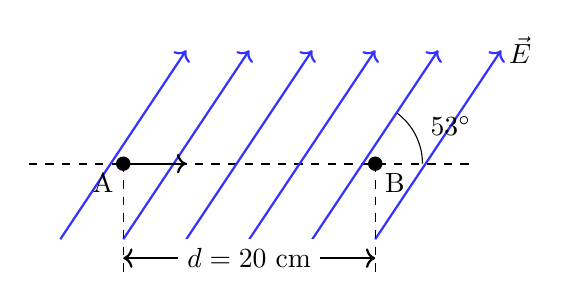
\begin{tikzpicture}[scale=0.8]
    % Gorizontal punktir chiziq
    \draw[dashed, thick] (-1,0) -- (6,0);

    % Elektr maydon chiziqlari (53 gradus burchak ostida parallel strelkalar)
    \foreach \x in {0,1,2,3,4,5} {
        \draw[->, thick, blue!80] (\x-0.5, -1.2) -- (\x+1.5, 1.8);
    }
    % Maydon kuchlanganligi belgisi
    \node at (6.8, 1.8) {$\vec{E}$};

    % A nuqta (zaryadlangan sharcha bilan)
    \filldraw (0.5,0) circle (3pt) node[below left] {A};
    % A nuqtadan yo'nalgan kichik tezlik/ko'chish strelkasi
    \draw[->, thick] (0.5,0) -- (1.5,0);

    % B nuqta
    \filldraw (4.5,0) circle (3pt) node[below right] {B};

    % 53 gradus burchakni ko'rsatish
    \draw (4.25,0) ++(0:1) arc (0:53:1);
    \node at (5.7,0.6) {$53^\circ$};

    % Masofani ko'rsatuvchi vertikal punktir chiziqlar
    \draw[dashed] (0.5,0) -- (0.5,-1.8);
    \draw[dashed] (4.5,0) -- (4.5,-1.8);

    % d=20 cm masofa ko'rsatkichi
    \draw[<->, thick] (0.5,-1.5) -- node[fill=white] {$d=20 \text{ cm}$} (4.5,-1.5);

\end{tikzpicture}
    
    \begin{enumerate}[label=\Alph*)]
        \item 900
        \item 600
        \item 450
        \item 300
        \item 200
    \end{enumerate}

    \item Elektrostatik maydonning potensiali 40 V bo‘lgan nuqtasidan potensiali –10 V bo‘lgan nuqtasiga $2 \cdot 10^{-7}$ C musbat zaryadni ko‘chirishda necha Joul ish bajariladi?
    \begin{enumerate}[label=\Alph*)]
        \item $2 \cdot 10^{-5}$
        \item $6 \cdot 10^{-6}$
        \item $1 \cdot 10^{-5}$
        \item $6 \cdot 10^{-7}$
        \item $1 \cdot 10^{-7}$
    \end{enumerate}

    \item Elektr maydon 1-nuqtadan 2-nuqtaga 1 C musbat zaryadni ko‘chirishda necha Joul ish bajaradi? Nuqtalar orasidagi potensiallar farqi 10 V.

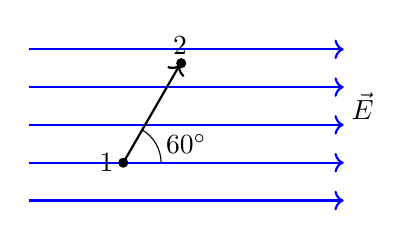
\begin{tikzpicture}[scale=0.8]
    % Elektr maydon chiziqlari (Gorizontal parallel strelkalar)
    \foreach \y in {0, 0.6, 1.2, 1.8, 2.4} {
        \draw[->, thick, blue] (-0.5, \y) -- (4.5, \y);
    }
    % Maydon kuchlanganligi belgisi
    \node at (4.8, 1.5) {$\vec{E}$};

    % Nuqtalarni belgilash (1-nuqta pastda, 2-nuqta yuqorida)
    \filldraw (1,0.6) circle (2pt);
    \filldraw (1.92,2.18) circle (2pt);
    \coordinate (P1) at (1, 0.6);
    \coordinate (P2) at ({1 + 1.8*cos(60)}, {0.6 + 1.8*sin(60)});

    % 1-nuqtadan 2-nuqtaga ko'chish chizig'i va yo'nalish strelkasi
    \draw[thick, ->] (P1) -- (P2);

    % Nuqta raqamlari
    \node[left] at (P1) {1};
    \node[above] at (P2) {2};

    % 60 gradus burchakni ko'rsatuvchi yoy
    \draw (1.6, 0.6) arc (0:60:0.6);
    \node at (2.0, 0.9) {$60^\circ$};

\end{tikzpicture}
    
    \begin{enumerate}[label=\Alph*)]
        \item 0
        \item 10
        \item 8,7
        \item 5
        \item 17
    \end{enumerate}

    \item $1,2 \cdot 10^{-4}$ C zaryadni bir nuqtadan ikkinchi nuqtaga ko‘chirishda 0,6 mJ ish bajarildi. Nuqtalar orasidagi potensiallar farqini aniqlang (V).
    \begin{enumerate}[label=\Alph*)]
        \item 10
        \item 5
        \item 3
        \item 0,7
        \item 0,5
    \end{enumerate}

    \item Elektronni elektr maydonda bir nuqtadan ikkinchi nuqtaga ko‘chirish natijasida uning kinetik energiyasi $8 \cdot 10^{-19}$ J ga o‘zgardi. Shu ikki nuqta orasidagi potensiallar farqini qanday (V). $e=1,6 \cdot 10^{-19}$ C.
    \begin{enumerate}[label=\Alph*)]
        \item 32
        \item 16
        \item 8
        \item 6
        \item 5
    \end{enumerate}

    \item Elektr maydonda elektronning tezligi $1 \cdot 10^7$ dan $5 \cdot 10^7$ m/s gacha oshdi. Boshlang‘ich va oxirgi nuqtalar orasidagi potensiallar ayirmasi qanday (kV)? Elektron zaryadining massasiga nisbati $1,76 \cdot 10^{11}$ C/kg.
    \begin{enumerate}[label=\Alph*)]
        \item 3,4
        \item 4
        \item 6
        \item 1,76
        \item 6,8
    \end{enumerate}

    
    \item Chizmada keltirilgan bir jinsli elektr maydondagi 2- va 3-nuqtalar orasidagi potensiallar farqi 6 V bo‘lsa, 1- va 3- nuqtalar orasida 3,5 $\mu$C zaryadni ko‘chirishda qanday ($\mu$J) ish bajariladi?

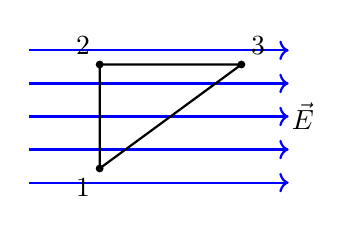
\begin{tikzpicture}[scale=0.6]
    % Elektr maydon chiziqlari (Gorizontal parallel strelkalar)
    \foreach \y in {0, 0.7, 1.4, 2.1, 2.8} {
        \draw[->, thick, blue] (-0.5, \y) -- (5, \y);
    }
    % Maydon kuchlanganligi belgisi
    \node at (5.3, 1.4) {$\vec{E}$};

    % Nuqtalarni belgilash (To'g'ri burchakli uchburchak)
    % 1-nuqta pastki chap burchakda
    % 2-nuqta 1 ning tepasida (vertikal)
    % 3-nuqta 2 ning o'ng tomonida (gorizontal)
    \coordinate (P1) at (1, 0.3);
    \coordinate (P2) at (1, 2.5);
    \coordinate (P3) at (4, 2.5);

    % Uchburchak chiziqlarini chizish
    \draw[thick] (P1) -- (P2) -- (P3) -- cycle;

    % Nuqtalarni kichik doira bilan belgilash
    \filldraw (P1) circle (2pt) node[below left] {1};
    \filldraw (P2) circle (2pt) node[above left] {2};
    \filldraw (P3) circle (2pt) node[above right] {3};

\end{tikzpicture}
    
    \begin{enumerate}[label=\Alph*)]
        \item 4
        \item $4\sqrt{2}$
        \item 21
        \item $8\sqrt{2}$
        \item 16
    \end{enumerate}

    \item Chizmada keltirilgan bir jinsli elektr maydondagi 1-, 2- va 3-nuqtalar teng tomonli uchburchakning uchlariga to‘g‘ri keladi. 1- va 3-nuqtalar orasidagi potensiallar farqi 16 V bo‘lsa, 2- va 3-nuqtalar orasida 2,5 $\mu$C zaryadni ko‘chirishda qanday ($\mu$J) ish bajariladi?

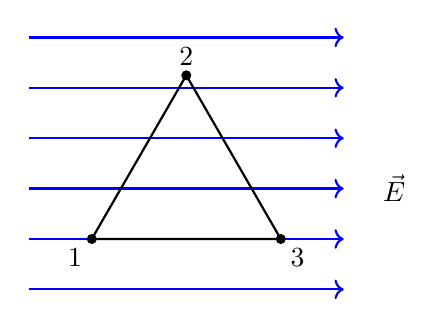
\begin{tikzpicture}[scale=0.8]
    % Elektr maydon chiziqlari (Gorizontal parallel strelkalar)
    \foreach \y in {0, 0.8, 1.6, 2.4, 3.2, 4} {
        \draw[->, thick, blue] (0, \y) -- (5, \y);
    }
    % Maydon kuchlanganligi belgisi
    \node at (5.8, 1.6) {$\vec{E}$};

    % Nuqtalarni belgilash (Teng tomonli uchburchak)
    % Uchburchak tomonini 3 birlik deb olsak:
    \coordinate (P1) at (1, 0.8); % Pastki chap nuqta
    \coordinate (P3) at (4, 0.8); % Pastki o'ng nuqta
    \coordinate (P2) at (2.5, {0.8 + 3*sin(60)}); % Yuqori cho'qqi

    % Uchburchak qirralarini chizish
    \draw[thick] (P1) -- (P2) -- (P3) -- cycle;

    % Nuqtalarni kichik doira bilan belgilash
    \filldraw (P1) circle (2pt) node[below left] {1};
    \filldraw (P2) circle (2pt) node[above] {2};
    \filldraw (P3) circle (2pt) node[below right] {3};

\end{tikzpicture}
    
    \begin{enumerate}[label=\Alph*)]
        \item 4
        \item 12
        \item 3
        \item 6
        \item 20
    \end{enumerate}

    \item Zaryadlangan ikkita tekislik (yassi kondensator) elektr maydonining turli nuqtalarida (1, 2, 3, 4) maydon kuchlanganliklari va potensiallari munosabati qanday?
    

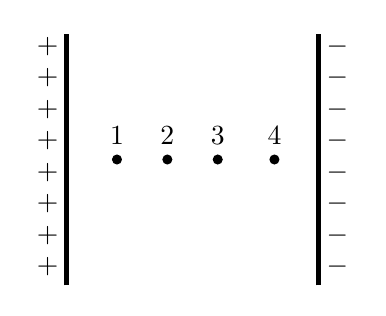
\begin{tikzpicture}[scale=0.8]
    % Musbat plastina (chapda)
    \draw[ultra thick] (0,0) -- (0,4);
    \foreach \y in {0.3, 0.8, ..., 3.8} {
        \node at (-0.3, \y) {$+$};
    }

    % Manfiy plastina (o'ngda)
    \draw[ultra thick] (4,0) -- (4,4);
    
    \foreach \y in {0.3, 0.8, ..., 3.8} {
        \node at (4.3, \y) {$-$};
    }

    % Nuqtalarni belgilash (1, 2, 3, 4)
    % Ular plastinalar orasida bitta gorizontal chiziqda yotadi
    \foreach \x/\n in {0.8/1, 1.6/2, 2.4/3, 3.3/4} {
        \filldraw (\x, 2) circle (2pt) node[above, yshift=2pt] {\n};
    }
    
\end{tikzpicture}

    \begin{enumerate}
    [label=\Alph*)]
        \item $E_1>E_2>E_3>E_4, \quad  \varphi_1=\varphi_2=\varphi_3=\varphi_4$
        \item $E_1<E_2<E_3<E_4, \quad \varphi_1<\varphi_2<\varphi_3<\varphi_4$
        \item $E_1=E_2=E_3=E_4, \quad \varphi_1>\varphi_2>\varphi_3>\varphi_4$
        \item $E_1=E_4>E_2=E_3, \quad \varphi_1=\varphi_4>\varphi_2=\varphi_3$
        \item $E_1<E_2=E_3<E_4, \quad \varphi_1<\varphi_2=\varphi_3<\varphi_4$
    \end{enumerate}

    \item Nuqtaviy musbat zaryadni bir jinsli elektrostatik maydonda O nuqtadan navbat bilan 1-, 2-, 3-, 4- nuqtalarga ko‘chirishda bajarilgan ishlar uchun quyidagi munosabatlarning qaysi biri to‘g‘ri?

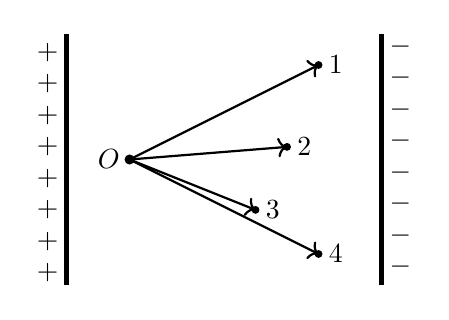
\begin{tikzpicture}[scale=0.8]
    % Chapdagi musbat zaryadlangan plastina
    \draw[ultra thick] (0,0) -- (0,4);
    \foreach \y in {0.2, 0.7, ..., 3.8} {
        \node at (-0.3, \y) {$+$};
    }
    
    \foreach \y in {0.3, 0.8, ..., 3.8} {
        \node at (5.3, \y) {$-$};
    }
    
    % O'ngdagi manfiy zaryadlangan plastina (punktir chiziq bilan)
    \draw[ultra thick] (5,0) -- (5,4);
    

    % O nuqtasi (boshlang'ich holat)
    \coordinate (O) at (1, 2);
    \filldraw (O) circle (2pt) node[left] {$O$};

    % Ko'chish nuqtalari (1, 2, 3, 4)
    % 1, 2 va 4-nuqtalar bir xil gorizontal masofada joylashgan
    \coordinate (P1) at (4, 3.5);
    \coordinate (P2) at (3.5, 2.2);
    \coordinate (P3) at (3, 1.2);
    \coordinate (P4) at (4, 0.5);

    % Yo'nalish strelkalari
    \draw[->, thick] (O) -- (P1) node[right] {1};
    \draw[->, thick] (O) -- (P2) node[right] {2};
    \draw[->, thick] (O) -- (P3) node[right] {3};
    \draw[->, thick] (O) -- (P4) node[right] {4};

    % Nuqtalarning o'zini belgilash
    \foreach \p in {P1, P2, P3, P4} {
        \filldraw (\p) circle (1.5pt);
    }
\end{tikzpicture}

    \begin{enumerate}[label=\Alph*)]
        \item $A_4>A_1>A_2>A_3$
        \item $A_1=A_4>A_2>A_3$
        \item $A_1=A_2=A_3=A_4$
        \item $A_1>A_4>A_2>A_3$
        \item $A_3>A_1=A_2>A_4$
    \end{enumerate}

    \item Biror nuqtaviy zaryaddan qaralayotgan nuqtagacha bo‘lgan masofa 4 marta ortganda zaryad potensiali qanday o‘zgaradi?
    \begin{enumerate}[label=\Alph*)]
        \item 4 marta kamayadi
        \item 4 marta ortadi
        \item 2 marta kamayadi
        \item 2 marta ortadi
        \item 16 marta ortadi
    \end{enumerate}

    \item Nuqtaviy zaryad maydon kuchlanganligi zaryaddan 3,5 cm masofadagi nuqtada 150 V/m bo‘lib, zaryad tomonga yo‘nalgan. Shu nuqtadagi maydon potensiali (V) nimaga teng?
    \begin{enumerate}[label=\Alph*)]
        \item -5,25
        \item -3,75
        \item 3,75
        \item 5,25
        \item 0
    \end{enumerate}

    \item $+q$ hamda $+2q$ nuqtaviy zaryadlar bir biridan $2r$ masofada turibdi. Ularning o‘rtasida joylashgan A nuqtadagi potensial 3 V ga teng. A nuqtadan $2r$ masofaga $Q$ nuqtaviy zaryad joylashtirilganda esa bu nuqtadagi potensial -3 V ni tashkil etdi. $Q$ zaryadni toping.

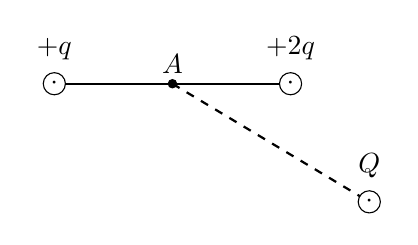
\begin{tikzpicture}[>=stealth, scale=1]
    % Asosiy gorizontal chiziq (+q va +2q orasida)
    \draw[thick] (-1.5,0) -- (1.5,0);

    % +q zaryadi (chapda)
    \filldraw[white, draw=black] (-1.5,0) circle (4pt);
    \node at (-1.5,0) {$\cdot$};
    \node[above, yshift=5pt] at (-1.5,0) {$+q$};

    % +2q zaryadi (o'ngda)
    \filldraw[white, draw=black] (1.5,0) circle (4pt);
    \node at (1.5,0) {$\cdot$};
    \node[above, yshift=5pt] at (1.5,0) {$+2q$};

    % A nuqtasi (o'rtada)
    \filldraw (0,0) circle (1.5pt) node[above] {$A$};

    % Q zaryadigacha bo'lgan punktir chiziq
    % Rasmga ko'ra A dan 2r masofada diagonal pastga yo'nalgan
    \draw[dashed, thick] (0,0) -- (2.5, -1.5);

    % Q zaryadi
    \filldraw[white, draw=black] (2.5,-1.5) circle (4pt);
    \node at (2.5,-1.5) {$\cdot$};
    \node[above, yshift=5pt] at (2.5,-1.5) {$Q$};

\end{tikzpicture}
    
    \begin{enumerate}[label=\Alph*)]
        \item $Q = -12q$
        \item $Q = -6q$
        \item $Q = 6q$
        \item $Q = 12q$
        \item $Q = q$
    \end{enumerate}

    \item $+2q$ va $-q$ zaryadlar rasmdagi kabi o‘rnatilgan. M va N nuqtalar orasidagi potensiallar farqi nimaga teng?

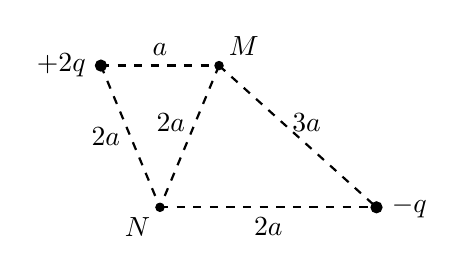
\begin{tikzpicture}[scale=1, >=stealth]
    % Nuqtalar koordinatalari (Rasmga mos nisbatda)
    \coordinate (Q1) at (0, 2);    % +2q zaryadi
    \coordinate (M)  at (1.5, 2);  % M nuqtasi
    \coordinate (N)  at (0.75, 0.2); % N nuqtasi
    \coordinate (Q2) at (3.5, 0.2); % -q zaryadi

    % Masofalarni ko'rsatuvchi punktir chiziqlar va label'lar
    \draw[dashed, thick] (Q1) -- node[above] {$a$} (M);
    \draw[dashed, thick] (Q1) -- node[left] {$2a$} (N);
    \draw[dashed, thick] (M) -- node[left, pos=0.4] {$2a$} (N);
    \draw[dashed, thick] (M) -- node[right, pos=0.4] {$3a$} (Q2);
    \draw[dashed, thick] (N) -- node[below] {$2a$} (Q2);

    % Zaryadlarni va nuqtalarni belgilash
    \filldraw (Q1) circle (2pt) node[left, xshift=-2pt] {$+2q$};
    \filldraw (M)  circle (1.5pt) node[above right] {$M$};
    \filldraw (N)  circle (1.5pt) node[below left] {$N$};
    \filldraw (Q2) circle (2pt) node[right, xshift=2pt] {$-q$};

\end{tikzpicture}
    
    \begin{enumerate}[label=\Alph*)]
        \item $2kq/a$
        \item $2kq/3a$
        \item $3kq/2a$
        \item $7kq/6a$
        \item 0
    \end{enumerate}

    \item $+3q$ va $+4q$ zaryadlar rasmdagi kabi o‘rnatilgan. M va N nuqtalar orasidagi potensiallar farqi nimaga teng?

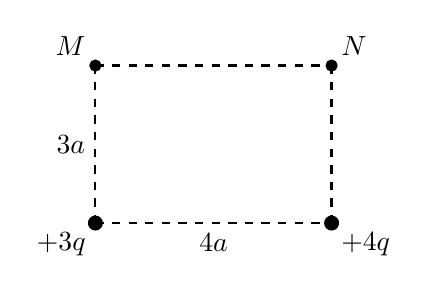
\begin{tikzpicture}
    % Nuqtalar koordinatalari
    \coordinate (M) at (0, 2);    % Yuqori chap nuqta
    \coordinate (N) at (3, 2);    % Yuqori o'ng nuqta
    \coordinate (Q1) at (0, 0);   % Pastki chap (+3q)
    \coordinate (Q2) at (3, 0);   % Pastki o'ng (+4q)

    % To'rtburchak tomonlarini ko'rsatuvchi punktir chiziqlar va masofalar
    \draw[dashed, thick] (M) -- node[left] {$3a$} (Q1);
    \draw[dashed, thick] (M) -- (N);
    \draw[dashed, thick] (N) -- (Q2);
    \draw[dashed, thick] (Q1) -- node[below] {$4a$} (Q2);

    % Nuqtalarni belgilash (M va N)
    \filldraw (M) circle (2pt) node[above left] {$M$};
    \filldraw (N) circle (2pt) node[above right] {$N$};

    % Zaryadlarni belgilash (+3q va +4q)
    \filldraw (Q1) circle (2.5pt) node[below left] {$+3q$};
    \filldraw (Q2) circle (2.5pt) node[below right] {$+4q$};

\end{tikzpicture}
    
    \begin{enumerate}[label=\Alph*)]
        \item $kq/15a$
        \item $2kq/15a$
        \item $kq/5a$
        \item $4kq/15a$
        \item $kq/3a$
    \end{enumerate}

    \item Rasmdagi to‘rtta zaryadning O nuqtadagi natijaviy elektr maydon kuchlanganligi 25 V/m ga teng bo‘lsa, shu nuqtadagi natijaviy potensiali necha Volt?

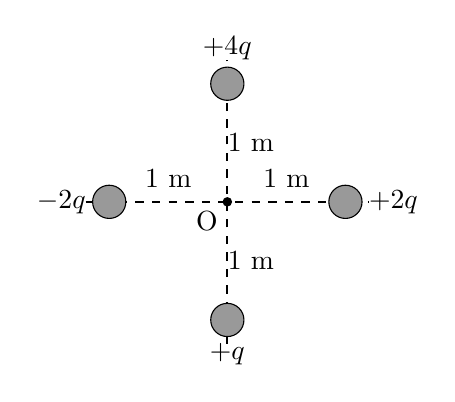
\begin{tikzpicture}[scale=1.5, >=stealth]
    % Koordinata o'qlari (punktir chiziqlar)
    \draw[dashed, thick] (0,-1.2) -- (0,1.2);
    \draw[dashed, thick] (-1.2,0) -- (1.2,0);

    % Markaziy O nuqtasi
    \filldraw (0,0) circle (1pt) node[below left] {O};
    
    \filldraw (0,0) circle (0.5pt);

    % Zaryadlarni joylashtirish va belgilash
    % Yuqorida +4q
    \filldraw[gray!80, draw=black] (0,1) circle (4pt) node[above, yshift=5pt, black] { $+4q$};
    % Pastda +q
    \filldraw[gray!80, draw=black] (0,-1) circle (4pt) node[below, yshift=-5pt, black] { $+q$};
    % Chapda -2q
    \filldraw[gray!80, draw=black] (-1,0) circle (4pt) node[left, xshift=-5pt, black] { $-2q$};
    % O'ngda +2q
    \filldraw[gray!80, draw=black] (1,0) circle (4pt) node[right, xshift=5pt, black] { $+2q$};

    % Masofalarni ko'rsatuvchi yozuvlar (1 m)
    \node at (0.2, 0.5) { $1\text{ m}$};
    \node at (0.2, -0.5) { $1\text{ m}$};
    \node at (-0.5, 0.2) { $1\text{ m}$};
    \node at (0.5, 0.2) { $1\text{ m}$};

\end{tikzpicture}
    
    \begin{enumerate}[label=\Alph*)]
        \item 25
        \item 30
        \item 35
        \item 40
        \item 50
    \end{enumerate}

    \item Radiuslari $R_1=R$ va $R_2=2R$ bo‘lgan metall sharlardagi zaryadning sirt zichligi bir xil. Sharlar markazlari-dagi potensiallarni solishtiring.
    \begin{enumerate}[label=\Alph*)]
        \item $\varphi_2=2\varphi_1$
        \item $\varphi_1=2\varphi_2$
        \item $\varphi_1=\varphi_2$
        \item $\varphi_1=4\varphi_2$
        \item $\varphi_2=4\varphi_1$
    \end{enumerate}

    \item Radiusi 10 cm va potensiali 200 V bo‘lgan zaryadlangan o‘tkazuvchi sfera markazidagi kuchlanganlik va potensial nimaga teng?
    \begin{enumerate}[label=\Alph*)]
        \item 0; 0
        \item 200 V/m; 200 V
        \item 200 V/m; 0
        \item 10 V/m; 100 V
        \item 0; 200 V
    \end{enumerate}

    \item Potensiali va radiusi rasmda ko‘rsatilgan x va y sharlar bir-biriga tekkizildi. Shundan so‘ng sharlarning potensiali nimaga teng bo‘lib qoladi?

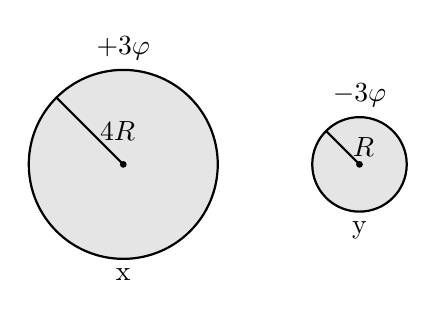
\begin{tikzpicture}[scale=1, >=stealth]
    % x shari (kattaroq)
    \draw[thick, fill=gray!20] (0,0) circle (1.2); % Radiusi 4R ni ifodalash uchun
    \filldraw (0,0) circle (1pt); % Markazi
    \draw[thick] (0,0) -- (-0.85, 0.85) node[midway, right] { $4R$}; % Radius chizig'i
    \node[above] at (0, 1.2) { $+3\varphi$}; % Potensiali
    \node[below] at (0, -1.2) {x}; % Shar nomi

    % y shari (kichikroq)
    \draw[thick, fill=gray!20] (3,0) circle (0.6); % Radiusi R ni ifodalash uchun
    \filldraw (3,0) circle (1pt); % Markazi
    \draw[thick] (3,0) -- (2.57, 0.43) node[midway, right] { $R$}; % Radius chizig'i
    \node[above] at (3, 0.6) {$-3\varphi$}; % Potensiali
    \node[below] at (3, -0.6) {y}; % Shar nomi

\end{tikzpicture}
    
    \begin{enumerate}[label=\Alph*)]
        \item 0
        \item $-2\varphi/3$
        \item $+\varphi$
        \item $+9\varphi/5$
        \item $+2\varphi$
    \end{enumerate}

    \item Rasmdagi K shar avval L sharga, keyin M sharga tekkizib olindi. Shundan so‘ng sharlarning zaryadi nimaga teng bo‘lib qoladi?

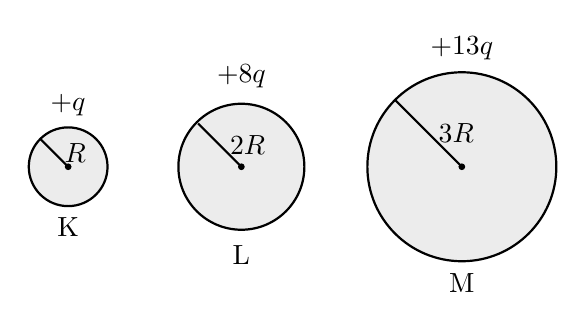
\begin{tikzpicture}[scale=1, >=stealth]
    % K shari (eng kichigi)
    \draw[thick, fill=gray!15] (0,0) circle (0.5); 
    \filldraw (0,0) circle (1pt); % Markazi
    \draw[thick] (0,0) -- (-0.35, 0.35) node[midway, right] {$R$}; % Radiusi
    \node[above, yshift=15pt] at (0,0) {$+q$}; % Zaryadi
    \node[below, yshift=-15pt] at (0,0) {K}; % Nomi

    % L shari (o'rtacha)
    \draw[thick, fill=gray!15] (2.2,0) circle (0.8); 
    \filldraw (2.2,0) circle (1pt); % Markazi
    \draw[thick] (2.2,0) -- (1.65, 0.55) node[midway, right] {$2R$}; % Radiusi
    \node[above, yshift=25pt] at (2.2,0) {$+8q$}; % Zaryadi
    \node[below, yshift=-25pt] at (2.2,0) {L}; % Nomi

    % M shari (eng kattasi)
    \draw[thick, fill=gray!15] (5,0) circle (1.2); 
    \filldraw (5,0) circle (1pt); % Markazi
    \draw[thick] (5,0) -- (4.15, 0.85) node[midway, right] {$3R$}; % Radiusi
    \node[above, yshift=35pt] at (5,0) {$+13q$}; % Zaryadi
    \node[below, yshift=-35pt] at (5,0) {M}; % Nomi

\end{tikzpicture}
    
    \begin{enumerate}[label=\Alph*)]
        \item $+q; +18q; +3q$
        \item $+6q; +q; +18q$
        \item $+4q; +6q; +12q$
        \item $+10q; +4q; +8q$
        \item $+2q; +12q; +6q$
    \end{enumerate}

    \item Rasmdagi K shar avval L sharga, keyin M sharga tekkizib olindi. Shundan so‘ng L sharning zaryadi nimaga teng bo‘lib qoladi?

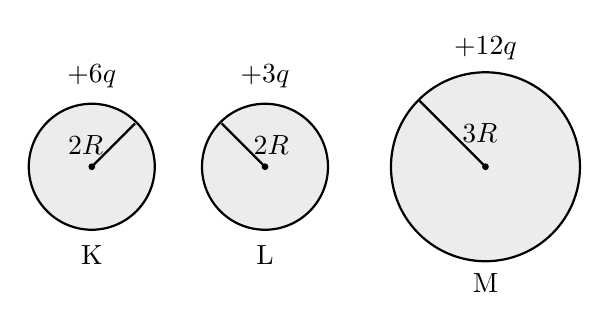
\begin{tikzpicture}[scale=1, >=stealth]
    % K shari (eng kichigi)
   \draw[thick, fill=gray!15] (0,0) circle (0.8); 
    \filldraw (0,0) circle (1pt); % Markazi
    \draw[thick] (0,0) -- (0.55, 0.55) node[midway, left] {$2R$}; % Radiusi
    \node[above, yshift=25pt] at (0,0) {$+6q$}; % Zaryadi
    \node[below, yshift=-25pt] at (0,0) {K}; % Nomi

    % L shari (o'rtacha)
    \draw[thick, fill=gray!15] (2.2,0) circle (0.8); 
    \filldraw (2.2,0) circle (1pt); % Markazi
    \draw[thick] (2.2,0) -- (1.65, 0.55) node[midway, right] {$2R$}; % Radiusi
    \node[above, yshift=25pt] at (2.2,0) {$+3q$}; % Zaryadi
    \node[below, yshift=-25pt] at (2.2,0) {L}; % Nomi

    % M shari (eng kattasi)
    \draw[thick, fill=gray!15] (5,0) circle (1.2); 
    \filldraw (5,0) circle (1pt); % Markazi
    \draw[thick] (5,0) -- (4.15, 0.85) node[midway, right] {$3R$}; % Radiusi
    \node[above, yshift=35pt] at (5,0) {$+12q$}; % Zaryadi
    \node[below, yshift=-35pt] at (5,0) {M}; % Nomi

\end{tikzpicture}
    
    \begin{enumerate}[label=\Alph*)]
        \item $+q$
        \item $+3q$
        \item $+2q$
        \item $+6q$
        \item $+5q$
    \end{enumerate}

\end{enumerate}
\section{Elektr sig`imi. Kondensatorlar}

\begin{enumerate}

\item O‘tkazgichning elektr sig‘imi deb ...
\begin{enumerate}[label=\Alph*)]
\item o‘tkazgich zaryadining potensialiga ko‘paytmasi bilan o‘lchanadigan kattalikka aytiladi.
\item o‘tkazgich zaryadiga to‘g‘ri proporsional va potensialiga teskari proporsional kattalikka aytiladi.
\item o‘tkazgich potensialining uning zaryadiga nisbatiga teng bo‘lgan kattalikka aytiladi.
\item o‘tkazgich zaryadining potensialiga nisbati bilan o‘lchanadigan kattalikka aytiladi.
\item TJY.
\end{enumerate}

\item Yakkalangan o‘tkazgichga $3\cdot10^{-9}$ C zaryad berilganda, uning potensiali $120$ V ga teng bo‘ldi. O‘tkazgichning elektr sig‘imini toping (F).
\begin{enumerate}[label=\Alph*)]
\item $2,5\cdot10^{-11}$
\item $4\cdot10^{-11}$
\item $3,6\cdot10^{-12}$
\item $3,6\cdot10^{-7}$
\item $5\cdot10^{-10}$
\end{enumerate}

\item Kondensatorning bir qoplamasining zaryadi $100$ nC, ikkinchisiniki esa $-100$ nC. Kondensatorning zaryadi necha nC?
\begin{enumerate}[label=\Alph*)]
\item 0
\item 100
\item 200
\item 1000
\item $10^4$
\end{enumerate}

\item Elektr sig‘imi $15$ nF bo‘lgan kondensatorning qoplamalari orasidagi potensiallar farqi $20$ V ga teng. Kondensatorning qoplamalaridan biridagi zaryad miqdorini toping (C).
\begin{enumerate}[label=\Alph*)]
\item 0,1
\item 0,3
\item 0,5
\item 3
\item 0,75
\end{enumerate}

\item $200$ V kuchlanishga ulangan, zaryadi $2\cdot10^{-4}$ C bo‘lgan kondensatorning sig‘imini toping ($\mu$F).
\begin{enumerate}[label=\Alph*)]
\item 0,1
\item 0,2
\item 0,4
\item 1
\item 2
\end{enumerate}

\item $300$ V o‘zgarmas kuchlanishga ulangan kondensator zaryadi $12\cdot10^{-4}$ C bo‘lsa, kondensatorning sig‘imi necha $\mu$F?
\begin{enumerate}[label=\Alph*)]
\item 0,1
\item 1
\item 2
\item 4
\item 7
\end{enumerate}

\item Sig‘imi $30$ pF bo‘lgan kondensator qoplamalariga berilgan zaryad miqdori $4,2\cdot10^{-8}$ C. Kondensator qanday kuchlanishgacha zaryadlangan (kV)?
\begin{enumerate}[label=\Alph*)]
\item 1,4
\item 34,2
\item 7
\item 2,8
\item 25,8
\end{enumerate}

\item Kondensatorning sig‘imi $4$ pF, qoplamalari orasidagi potensiallar ayirmasi $200$ V bo‘lsa, har bir qoplamada necha Kulon zaryad bor?
\begin{enumerate}[label=\Alph*)]
\item $6\cdot10^{-10}$
\item $2\cdot10^{-10}$
\item $2\cdot10^{-9}$
\item $8\cdot10^{-10}$
\item $4\cdot10^{-10}$
\end{enumerate}

\item Yassi kondensatorning bir plastinkasiga $+0,2$ C, ikkinchi plastinkasiga $-0,2$ C zaryad berilgan. Plastinkalar orasidagi kuchlanish $5$ kV. Kondensator sig‘imi qanday ($\mu$F)?
\begin{enumerate}[label=\Alph*)]
\item 80
\item 40
\item 25
\item 10
\item 0
\end{enumerate}

\item Kondensator qoplamalaridan biridagi potensial $300$ V, ikkinchisidagi esa $-300$ V va qoplamalardan biridagi zaryad $2,4$ $\mu$C bo‘lsa, uning sig‘imini toping (nF).
\begin{enumerate}[label=\Alph*)]
\item 8
\item 4
\item 5
\item 3
\item 10
\end{enumerate}

\item BXS dagi o‘lchamligi J/V$^2$ bo‘lgan fizik kattalik birligining nomi nima?
\begin{enumerate}[label=\Alph*)]
\item Kulon
\item Farad
\item Om
\item Amper
\item Nyuton
\end{enumerate}

\item Quyidagi birliklarning qaysilari elektr sig‘im birligi sifatida ishlatsa bo‘ladi:\\
1) F, \quad 2) C$^2$/J, 3) \quad 3) J/V$^2$, \quad 4) C/V.

\begin{enumerate}[label=\Alph*)]
\item 1, 4
\item 1, 2
\item hammasini
\item 1, 2, 3
\item 3, 4
\end{enumerate}

\item Yakkalangan shar elektr sig‘imi ifodasini ko‘rsating.
\begin{enumerate}[label=\Alph*)]
\item $C=\dfrac{\varphi_1-\varphi_2}{q}$
\item $C=\dfrac{\varepsilon\varepsilon_0S}{d}$
\item $C=2\pi\varepsilon\varepsilon_0R$
\item $C=4\pi\varepsilon\varepsilon_0R$
\item $C=4\pi\varepsilon R$
\end{enumerate}

\item Necha metr radiusli sharning elektr sig‘imi vakuumda $1$ F ga teng bo‘ladi?
\begin{enumerate}[label=\Alph*)]
\item $1\cdot10^7$
\item $1\cdot10^8$
\item $9\cdot10^{10}$
\item $1\cdot10^9$
\item $9\cdot10^9$
\end{enumerate}

\item O‘tkazgichga boshqa o‘tkazgich yaqinlashtirilganda, uning sig‘imi qanday o‘zgaradi?
\begin{enumerate}[label=\Alph*)]
\item ortadi
\item o‘zgarmaydi
\item kamayadi
\item avval ortadi, so‘ngra kamayadi
\item avval kamayadi, so‘ngra ortadi
\end{enumerate}

\item Zaryadlangan kondensator qoplamalari sim bilan tutashtirilib, zaryadsizlantirildi. Bunda qoplamalar massasi qanday o‘zgaradi?
\begin{enumerate}[label=\Alph*)]
\item har ikkala qoplamaning massasi ortadi.
\item musbat zaryadlangan qoplama massasi ortib, manfiy zaryadlangan qoplama massasi kamayadi.
\item har ikkala qoplamaning massasida o‘zgarish bo‘lmaydi.
\item manfiy zaryadlangan qoplama massasi ortib, musbat zaryadlangan qoplama massasi kamayadi.
\item har ikkala qoplamaning massasi kamayadi.
\end{enumerate}

\item Keltirilgan tenglamalardan qaysi biri yassi kondensator elektr sig‘imini ifodalaydi?
\begin{enumerate}[label=\Alph*)]
\item $C=C_1+C_2+\ldots+C_n$
\item $C=4\pi\varepsilon_0R$
\item $C=\dfrac{q}{U}$
\item $C=\dfrac{Q}{m(t_2-t_1)}$
\item $C=\dfrac{\varepsilon\varepsilon_0S}{d}$
\end{enumerate}

\item Yassi kondensator qoplamalarining yuzasi $40$ cm$^2$ dan, qoplamalari orasidagi masofa esa $5$ mm ga teng. Qoplamalar orasidagi muhitning dielektrik singdiruvchanligi $5$ ga teng bo‘lsa, uning sig‘imini toping (pF).
\begin{enumerate}[label=\Alph*)]
\item 12,46
\item 23,77
\item 15,1
\item 26,9
\item 35,4
\end{enumerate}

\item Sig‘imi $20$ pF bo‘lgan yassi kondensator har bir qoplamasining yuzasi $20$ cm$^2$ dan, qoplamalari orasidagi masofa esa $8,85$ mm ga teng. Qoplamalar orasidagi muhitning dielektrik singdiruvchanligini toping.
\begin{enumerate}[label=\Alph*)]
\item 8
\item 4
\item 5
\item 3
\item 10
\end{enumerate}

\item Sig‘imi $8,85$ pF bo‘lgan yassi kondensator har bir qoplamasining yuzasi $10$ cm$^2$ dan va qoplamalari orasidagi muhitning dielektrik singdiruvchanligi $3$ ga teng bo‘lsa, qoplamalari orasidagi masofani toping (mm).
\begin{enumerate}[label=\Alph*)]
\item 1
\item 4
\item 2
\item 3
\item 5
\end{enumerate}

\item Har bir qoplamasidagi zaryad miqdori $88,5$ $\mu$C bo‘lgan yassi kondensator qoplamalarining yuzasi $50$ cm$^2$ dan, qoplamalari orasidagi masofa $5$ mm va qoplamalari orasidagi muhitning dielektrik singdiruvchanligi $2,5$ ga teng bo‘lsa, qoplamalar orasidagi potensiallar farqini toping (MV).
\begin{enumerate}[label=\Alph*)]
\item 1
\item 4
\item 2
\item 3
\item 5
\end{enumerate}

\item Qoplamalari orasidagi kuchlanish $20$ kV bo‘lgan yassi kondensator qoplamalarining yuzasi $2$ cm$^2$ dan, qoplamalari orasidagi masofa $35,4$ mm va qoplamalari orasidagi muhitning dielektrik singdiruvchanligi $40$ ga teng bo‘lsa, har bir qoplamadagi zaryad miqdorini toping ($\mu$C).
\begin{enumerate}[label=\Alph*)]
\item 0,04
\item 0,03
\item 0,02
\item 0,15
\item 0,25
\end{enumerate}

\item Yassi kondensator qoplamalari diametri $0,2$ m dan bo‘lgan ikkita doiraviy plastinadan iborat. Qoplamalar orasidagi havo qatlamining qalinligi $3\cdot10^{-3}$ m, qoplamalar orasidagi kuchlanish $120$ V. Qoplamalardan har biridagi zaryad necha Kulon?
\begin{enumerate}[label=\Alph*)]
\item $1,55\cdot10^{-8}$
\item $1,22\cdot10^{-8}$
\item $0,82\cdot10^{-8}$
\item $1,01\cdot10^{-8}$
\item $1,06\cdot10^{-8}$
\end{enumerate}

\item Kondensator zaryadi 2 marta ortganda, uning sig‘imi qanday o‘zgaradi?
\begin{enumerate}[label=\Alph*)]
\item 4 marta kamayadi.
\item 2 marta oshadi.
\item 2 marta kamayadi.
\item 4 marta oshadi.
\item o‘zgarmaydi.
\end{enumerate}

\item Kondensator qoplamalaridagi zaryad 4 marta orttirilsa, uning sig‘imi qanday o‘zgaradi?
\begin{enumerate}[label=\Alph*)]
\item 4 marta kamayadi.
\item 2 marta ortadi.
\item 2 marta kamayadi.
\item 4 marta ortadi.
\item o‘zgarmaydi.
\end{enumerate}

\item Kondensator qoplamalari orasidagi kuchlanish 2 marta ortganda, uning sig‘imi qanday o‘zgaradi?
\begin{enumerate}[label=\Alph*)]
\item 2 marta kamayadi.
\item 2 marta ortadi.
\item o‘zgarmaydi.
\item 4 marta ortadi.
\item 4 marta kamayadi.
\end{enumerate}

\item Yassi kondensator qoplamasining yuzi 2 marta ortganda, uning sig‘imi qanday o‘zgaradi?
\begin{enumerate}[label=\Alph*)]
\item 2 marta kamayadi.
\item 4 marta ortadi.
\item o‘zgarmaydi.
\item 4 marta kamayadi.
\item 2 marta ortadi.
\end{enumerate}

\item Uchta yassi kondensator qoplamalarining yuzlari bir xil, ular orasidagi masofalar $d_1<d_2<d_3$ munosabatda bo‘lsa, sig‘imlarining munosabati qanday bo‘ladi?
\begin{enumerate}[label=\Alph*)]
\item $C_2<C_3<C_1$.
\item $C_1<C_2<C_3$.
\item $C_1=C_2=C_3$.
\item $C_1>C_3>C_2$.
\item $C_3<C_1<C_2$.
\end{enumerate}

\item Yassi havo kondensatori plastinalari orasidagi fazoga uchinchi plastina kiritilsa, sig‘imi qanday o‘zgaradi?
\begin{enumerate}[label=\Alph*)]
\item plastinaning dielektrik singdiruvchanligiga bog‘liq.
\item ortadi.
\item kamayadi.
\item o‘zgarmaydi.
\item TJY.
\end{enumerate}

\item Kondensator qoplamalari orasiga qalinligi qoplamalar orasidagi masofaning yarmiga teng bo‘lgan o‘tkazuvchi plastina kiritildi. Bunda kondensatorning sig‘imi qanday o‘zgaradi?
\begin{enumerate}[label=\Alph*)]
\item 4 marta ortadi.
\item 4 marta kamayadi.
\item o‘zgarmaydi.
\item 2 marta kamayadi.
\item 2 marta ortadi.
\end{enumerate}

\item Yassi kondensatorning har bir qoplamasi yuzi $S$, ular orasidagi masofa $d$. Qalinligi $l$ bo‘lgan metall plastina qoplamalarga tekkizilmagan holda kondensator ichiga kiritilgan. Kondensatorning sig‘imi qanday?
\begin{enumerate}[label=\Alph*)]
\item $\dfrac{\varepsilon_0 S}{2(d-l)}$
\item $\dfrac{\varepsilon_0 S}{d+l}$
\item $\dfrac{2\varepsilon_0 S}{d-l}$
\item $\dfrac{\varepsilon_0 S}{2(d+l)}$
\item $\dfrac{\varepsilon_0 S}{d-l}$
\end{enumerate}

\item Havo kondensatori qoplamalari orasidagi fazo hajmi $2$ m$^3$, uning sig‘imi $5$ nF. Agar hajmi $4$ m$^3$ gacha oshirilsa, kondensatorning sig‘imi qanday (nF) bo‘ladi?
\begin{enumerate}[label=\Alph*)]
\item 10
\item 15
\item 2,5
\item aniqlab bo‘lmaydi.
\item 5
\end{enumerate}

\item Yassi kondensator plastinalari orasidagi masofa $6$ marta, har bir plastinaning yuzi $3$ marta kamaytirilsa, kondensator sig‘imi qanday o‘zgaradi?
\begin{enumerate}[label=\Alph*)]
\item 2 marta ortadi.
\item 6 marta kamayadi.
\item 3 marta kamayadi.
\item 6 marta ortadi.
\item 3 marta ortadi.
\end{enumerate}

\item Yassi kondensator qoplamalari orasiga $\varepsilon=2$ bo‘lgan dielektrik bilan to‘ldirilsa, uning sig‘imi qanday o‘zgaradi?
\begin{enumerate}[label=\Alph*)]
\item o‘zgarmaydi.
\item 2 marta kamayadi.
\item 2 marta oshadi.
\item 4 marta kamayadi.
\item 4 marta oshadi.
\end{enumerate}

\item Uchta bir xil yassi kondensator qoplamalari orasiga turli dielektriklar joylashtirilgan: $\varepsilon_1<\varepsilon_2<\varepsilon_3$. Kondensatorlarning sig‘imlari qanday munosabatda bo‘ladi?
\begin{enumerate}[label=\Alph*)]
\item $C_3>C_2<C_1$.
\item $C_1>C_2>C_3$.
\item $C_1=C_2=C_3$.
\item $C_1<C_2<C_3$.
\item $C_1>C_2<C_3$.
\end{enumerate}

\item Yassi kondensator qoplamalari orasidagi masofa $4$ marta qisqartirilib, singdiruvchanligi $5$ ga teng bo‘lgan dielektrik o‘rniga, singdiruvchanligi $10$ ga teng bo‘lgan dielektrik joylashtirildi. Bunda kondensator sig‘imi qanday o‘zgaradi?
\begin{enumerate}[label=\Alph*)]
\item 4 marta kamayadi.
\item 8 marta ortadi.
\item 2 marta kamayadi.
\item 2 marta ortadi.
\item 8 marta kamayadi.
\end{enumerate}

\item O‘zgarmas tok manbaiga ulangan yassi kondensator plastinalari orasidagi masofa 2 marta oshirilsa, plastinalardagi zaryad miqdori qanday o‘zgaradi?
\begin{enumerate}[label=\Alph*)]
\item 4 marta kamayadi.
\item 2 marta oshadi.
\item o‘zgarmaydi.
\item 2 marta kamayadi.
\item 4 marta oshadi.
\end{enumerate}

\item Havo oraliqli yassi kondensator o‘zgarmas tok manbaidan zaryadlandi va undan uzildi. Plastinalar orasidagi masofa 2 marta kattalashtirilsa, kondensator zaryadi va kuchlanishi qanday o‘zgaradi?
\begin{enumerate}[label=\Alph*)]
\item zaryad va kuchlanish o‘zgarmaydi.
\item zaryad 2 marta ortadi, kuchlanish o‘zgarmaydi.
\item zaryad o‘zgarmaydi, kuchlanish 2 marta ortadi.
\item zaryad o‘zgarmaydi, kuchlanish 2 marta kamayadi.
\item zaryad 2 marta kamayadi, kuchlanish o‘zgarmaydi.
\end{enumerate}

\item Zaryadlangan kondensatorni manbadan uzib, plastinalari orasidagi masofa 7 marta kamaytirilsa, kuchlanishi qanday o‘zgaradi?
\begin{enumerate}[label=\Alph*)]
\item o‘zgarmaydi.
\item 7 marta ortadi.
\item 7 marta kamayadi.
\item 49 marta ortadi.
\item 49 marta kamayadi.
\end{enumerate}

\item Kondensator zaryadlanib, manbadan uzildi, so‘ngra u $\varepsilon=3$ bo‘lgan dielektrik bilan to‘ldirildi. Kondensatordagi kuchlanish qanday o‘zgaradi?
\begin{enumerate}[label=\Alph*)]
\item 9 marta ortadi.
\item 9 marta kamayadi.
\item o‘zgarmaydi.
\item 3 marta ortadi.
\item 3 marta kamayadi.
\end{enumerate}

\item Manbadan uzib qo‘yilgan zaryadlangan yassi kondensator plastinalari orasidagi masofa 2 marta oshirilsa, kondensatorning elektr maydon kuchlanganligi qanday o‘zgaradi?
\begin{enumerate}[label=\Alph*)]
\item o‘zgarmaydi.
\item 2 marta kamayadi.
\item 4 marta ortadi.
\item 4 marta kamayadi.
\item 2 marta ortadi.
\end{enumerate}

\item Agar zaryadlangan yassi havo kondensatorini manbadan uzib, qoplamalari orasidagi masofa 4 marta kamaytirilsa, undagi elektr maydon kuchlanganligi qanday o‘zgaradi?
\begin{enumerate}[label=\Alph*)]
\item o‘zgarmaydi.
\item 4 marta kamayadi.
\item 4 marta oshadi.
\item 16 marta kamayadi.
\item 16 marta oshadi.
\end{enumerate}

\item Yassi kondensator o‘zgarmas kuchlanish manbaiga ulandi. Qoplamalar orasidagi fazo dielektrik bilan to‘ldirilsa, kondensator ichidagi elektr maydon kuchlanganligi qanday o‘zgaradi?
\begin{enumerate}[label=\Alph*)]
\item kamayadi.
\item ortadi.
\item o‘zgarmaydi.
\item ortishi ham mumkin, kamayishi ham.
\item javob dielektrikning singdiruvchanligiga bog‘liq.
\end{enumerate}

\item Zaryadlangan kondensator qoplamalari bir-biriga $F$ kuch bilan tortiladilar. Agar qoplamalar orasiga dielektrik singdiruvchanligi $\varepsilon=2$ bo‘lgan yassi shisha plastina kiritilsa, bu kuch qanday o‘zgaradi? Plastina qalinligi qoplamalar orasidagi masofadan kichik bo‘lsin.
\begin{enumerate}[label=\Alph*)]
\item 2 marta kamayadi.
\item 2 marta ortadi.
\item 4 marta kamayadi.
\item 4 marta ortadi.
\item o‘zgarmaydi.
\end{enumerate}

\item Yassi havo kondensatori qoplamalari orasidagi masofa $8,85$ mm, zaryadining sirt zichligi $10^{-6}$ C/m$^2$ bo‘lsa, uning kuchlanishini necha Volt bo‘ladi?
\begin{enumerate}[label=\Alph*)]
\item 100
\item 500
\item 885
\item 1000
\item 2000
\end{enumerate}

\item Yassi havo kondensatori $9$ kV kuchlanishga ega bo‘lgan tok manbaiga ulangan. Kondensator plastinkalari orasidagi maydon kuchlanganligi $3$ MV/m bo‘lganda, havoda ionizatsiya tufayli teshilish yuz bersa, kondensator ishdan chiqmasligi uchun uning qoplamalarini qanday minimal masofaga yaqinlashtirish mumkin (mm)?
\begin{enumerate}[label=\Alph*)]
\item 1,5
\item 3
\item 15
\item 30
\item 60
\end{enumerate}


\end{enumerate}
\begin{table}[h!]
\centering
\begin{tabular}{|c|c|c|c|c|c|c|c|c|c|}
\hline
1d & 2a & 3b & 4b & 5d & 6d & 7a & 8d & 9b & 10b \\ \hline
11b & 12c & 13d & 14e & 15a & 16b & 17e & 18e & 19e & 20d \\ \hline
21b & 22a & 23e & 24e & 25e & 26c & 27e & 28d & 29b & 30e \\ \hline
31e & 32d & 33a & 34c & 35d & 36b & 37d & 38c & 39c & 40e \\ \hline
41a & 42a & 43c & 44e & 45d & 46b &  &  &  &  \\ \hline
\end{tabular}
\end{table}
\section{Kondensatorlarni parallel v aketma ket ulash}


\begin{enumerate}

\item 100 nF, 200 nF va 500 nF sig‘imli uchta kondensatorni ketma-ket ulangandagi umumiy sig‘imini toping (nF).
\begin{enumerate}[label=\Alph*)]
\item 800
\item 500
\item 100
\item 58,8
\end{enumerate}

\item Elektr sig‘imlari bir xil bo‘lgan uchta kondensator 2 V kuchlanish manbaiga parallel ulandi. Bunda har bir kondensator 1 nC zaryadga ega bo‘ldi. Zanjirning umumiy sig‘imini toping (pF).
\begin{enumerate}[label=\Alph*)]
\item 1400
\item 1500
\item 1600
\item 800
\end{enumerate}

\item Elektr sig‘imi 6 $\mu F$, 2 $\mu F$ va 4 $\mu F$ ga teng bo‘lgan kondensatorlar 24 V kuchlanish manbaiga ketma-ket ulangan. Ikkinchi kondensator qoplamalari orasidagi potensiallar farqini toping (V).
\begin{enumerate}[label=\Alph*)]
\item 8
\item 12
\item 4
\item 13,1
\end{enumerate}

\item O‘zgarmas tok manbaiga ulangan 8 $\mu F$ sig‘imli kondensatorga parallel ulangan voltmetr 6 V kuchlanishni ko‘rsatdi. Agar bu kondensatorga 2 $\mu F$ sig‘imli ikkinchi kondensator ketma-ket ulansa, voltmetr qanday kuchlanishni (V) ko‘rsatadi?
\begin{enumerate}[label=\Alph*)]
\item 1,2
\item 2
\item 6
\item 4,6
\end{enumerate}

\item $C_1 = 1 \, \mu F$ va $C_2 = 3 \, \mu F$ sig‘imli ikki kondensatorni ketma-ket ulab hosil qilingan elektr sxema $U = 220 \, V$ li o‘zgarmas kuchlanish manbaiga ulangan. Har bir kondensatordagi kuchlanishni aniqlang (V).
\begin{enumerate}[label=\Alph*)]
\item 115; 105
\item 120; 100
\item 145; 65
\item 165; 55
\end{enumerate}

\item 3 $\mu F$ va 6 $\mu F$ sig‘imli kondensatorlar o‘zaro ulangan va 120 V EYUK li batareyaga biriktirilgan. Agar kondensatorlar ketma-ket ulangan bo‘lsa, ularning qoplamalari orasidagi potensiallar farqi aniqlansin (V).
\begin{enumerate}[label=\Alph*)]
\item 80; 40
\item 80; 80
\item 40; 40
\item 80; 20
\end{enumerate}

\item  Rasmda tasvirlangan kondensatorlar tizimining umumiy sig‘imini toping.

\begin{circuitikz}[scale=0.8, transform shape]
  % Kirish terminali va 4C kondensator
  \draw (0,0) to [short, o-] (0.5,0)
        to [C, l=$4C$] (2,0);
  
  % Birinchi tugun va 3C kondensatorlar (Parallel)
  \draw (2,0) -- (2,1)
        to [C, l=$3C$] (4,1);
  \draw (2,0) -- (2,-1)
        to [C, l=$3C$] (4,-1);
        
  % 3C larning chiqishini bitta nuqtaga birlashtirish
  \draw (4,1) -- (4,-1);
  
  % Ikkinchi tugun va uchta 2C kondensatorlar (Parallel)
  \draw (4,1) to [C, l=$2C$] (6,1);
  \draw (4,0) to [C, l=$2C$] (6,0);
  \draw (4,-1) to [C, l=$2C$] (6,-1);
  
  % Barcha 2C larning chiqishini birlashtirish va chiqish terminali
  \draw (6,1) -- (6,-1);
  \draw (6,0) to [short, -o] (7,0);

  % Nuqtalarni belgilash (ixtiyoriy)
  \node[circle, fill, inner sep=1pt] at (2,0) {};
  \node[circle, fill, inner sep=1pt] at (4,0) {};
  \node[circle, fill, inner sep=1pt] at (6,0) {};
\end{circuitikz}

\begin{enumerate}[label=\Alph*)]
\item $47C/16$
\item $14C/15$
\item $15C/7$
\item $12C/7$
\end{enumerate}

\item  Sxemadan umumiy sig‘imni toping.
\begin{enumerate}[label=\Alph*)]
\item $3C/2$
\item $3C$
\item $6C$
\item $2C$
\end{enumerate}

\item  Rasmda har bir kondensatorning sig‘imi C ga teng. M va N nuqtalar orasidagi potensiallar farqi 120 V bo‘lsa, K va L nuqtalar orasidagi potensiallar farqini (V) toping.
\begin{enumerate}[label=\Alph*)]
\item 60
\item 40
\item 20
\item 30
\end{enumerate}

\item  Sig‘imlari $C_1 = 3 \, \mu F, C_2 = 5 \, \mu F, C_3 = 6 \, \mu F$ va $C_4 = 5 \, \mu F$ bo‘lgan to‘rtta kondensator rasmda ko‘rsatilgan sxema bo‘yicha ulangan. Batareyaning umumiy sig‘imini aniqlang ($\mu F$).
\begin{enumerate}[label=\Alph*)]
\item 2
\item 3,4
\item 9
\item 4,5
\end{enumerate}

\item  Rasmda ko‘rsatilgan kondensatorlar batareyasining A va B nuqtalar orasidagi elektr sig‘imini aniqlang.
\begin{enumerate}[label=\Alph*)]
\item 0,4C
\item 0,2C
\item C
\item 0,8C
\end{enumerate}

\item  Rasmdagi kondensatorlar batareyasining sig‘imi 5,8 $\mu F$ ga teng. Agar $C_2 = 1 \, \mu F, C_3 = 4 \, \mu F$ bo‘lsa, birinchi kondensatorning sig‘imi ($\mu F$) va undagi zaryad qanday ($\mu C$)?
\begin{enumerate}[label=\Alph*)]
\item 5; 1,1
\item 10; 1,1
\item 5; 0,8
\item 1,4; 3
\end{enumerate}

\item  Rasmdagi zanjirda K va L uchlar orasidagi zaryad miqdori Q ga teng. MN uchlari orasiga ulangan C sig‘imli kondensatorning zaryadi nimaga teng?
\begin{enumerate}[label=\Alph*)]
\item $Q/5$
\item $Q/2$
\item $8Q/53$
\item $13Q/40$
\end{enumerate}

\item Rasmda tasvirlangan kondensatorlar tizimining umumiy sig‘imini toping.
\begin{enumerate}[label=\Alph*)]
\item 3C
\item 6C/11
\item 5C/11
\item 6C
\end{enumerate}

\item  Ketma-ket ulangan ikkita bir xil kondensator modda bilan ikki xil usulda yarmigacha to‘ldirilgan. Bunda kondensator kuchlanishlarining farqi qanday bo‘ladi (V)?
\begin{enumerate}[label=\Alph*)]
\item 0
\item 24
\item 28,5
\item 12,6
\end{enumerate}

\item  Rasmda ko‘rsatilgan kondensatorlar batareyasida a va b nuqtalar orasidagi kuchlanishini toping (V).
\begin{enumerate}[label=\Alph*)]
\item 0
\item 8,25
\item 7,75
\item 5,33
\end{enumerate}

\item Sig‘imi 3 $\mu F$ zaryadi 5 $\mu C$ va sig‘imi 8 $\mu F$ zaryadi 3 $\mu C$ bo‘lgan kondensatorlar mos qutblari bilan ulangandan keyin, birinchi kondensatordagi zaryadni toping ($\mu C$).
\begin{enumerate}[label=\Alph*)]
\item 24/11
\item 64/11
\item 6/11
\item 16/11
\end{enumerate}

\item Sig‘imi 3 $\mu F$ zaryadi 5 $\mu C$ va sig‘imi 8 $\mu F$ zaryadi 3 $\mu C$ bo‘lgan kondensatorlar mos qutblari bilan ulangandan keyin, ikkinchi kondensatordagi zaryadni toping ($\mu C$).
\begin{enumerate}[label=\Alph*)]
\item 24/11
\item 64/11
\item 6/11
\item 16/11
\end{enumerate}

\item $C$ sig‘imli ikki kondensator $2U$ va $U$ kuchlanish bilan zaryadlangan. Agar kondensator qutblari teskari holda ulansa, natijaviy kuchlanish qanday bo‘ladi?
\begin{enumerate}[label=\Alph*)]
\item 4U
\item 2,5U
\item 2U
\item 0,5U
\end{enumerate}

\item $10^4 \, nF$ sig‘imli ikki kondensator 5 V va 10 V kuchlanish bilan zaryadlangan. Ularning qutblari mos ravishda ulansa, natijaviy kuchlanish qanday bo‘ladi?
\begin{enumerate}[label=\Alph*)]
\item 5
\item 12,5
\item 7,5
\item 50
\end{enumerate}

\item Bir xil zaryadlangan $C$ va $2C$ sig‘imli kondensatorlar o‘zaro parallel ulansa, birinchi kondensatordagi kuchlanish qanday o‘zgaradi?
\begin{enumerate}[label=\Alph*)]
\item o‘zgarmaydi
\item 1,5 marta ortadi
\item 1,5 marta kamayadi
\item 3 marta ortadi
\end{enumerate}

\item 800 V potensiallar farqigacha zaryadlangan havo kondensatori o‘lchamlari birday bo‘lgan dielektrikli zaryadlanmagan kondensator bilan parallel ulangan. Potensiallar farqi 100 V bo‘lsa, dielektrikning singdiruvchanligini toping.
\begin{enumerate}[label=\Alph*)]
\item 7
\item 2
\item 16
\item 3
\end{enumerate}

\item Yassi havo kondensatori 50 V gacha zaryadlangan va manbadan uzilgan. Qoplamalar orasiga 1 mm qalinlikdagi metall list kiritildi. Masofa 5 mm bo‘lsa, yangi potensiallar farqini aniqlang (V).
\begin{enumerate}[label=\Alph*)]
\item 30
\item 15
\item 80
\item 40
\end{enumerate}

\item Ikkita bir xil kondensator parallel ulangan va 6 V gacha zaryadlangan. Uzilgach, birining plastinkalari orasidagi masofa 2 marta kamaytirilsa, yangi potensiallar farqi qancha (V)?
\begin{enumerate}[label=\Alph*)]
\item 6
\item 2
\item 4
\item 12
\end{enumerate}

\item 12 $\mu F$ sig‘imli kondensatorga parallel voltmetr 3 V ni ko‘rsatmoqda. Unga 8 $\mu F$ sig‘imli ikkinchi kondensator parallel ulansa, voltmetr necha V ni ko‘rsatadi?
\begin{enumerate}[label=\Alph*)]
\item 1,5
\item 3
\item 1
\item 2
\end{enumerate}

\end{enumerate}



\begin{table}[h!]
\centering
\begin{tabular}{|c|c|c|c|c|c|c|c|c|c|}
\hline
№ & J. & № & J. & № & J. & № & J. & № & J. \\ \hline
1 & D & 6 & A & 11 & A & 16 & D & 21 & C \\ \hline
2 & B & 7 & D & 12 & A & 17 & A & 22 & A \\ \hline
3 & D & 8 & A & 13 & D & 18 & B & 23 & D \\ \hline
4 & A & 9 & B & 14 & D & 19 & D & 24 & C \\ \hline
5 & D & 10 & D & 15 & D & 20 & C & 25 & B \\ \hline
\end{tabular}
\end{table}
\section{O`zgarmas tok}



\begin{enumerate}

\item 800 V potensiallar farqigacha zaryadlangan havo kondensatori o‘lchamlari jihatidan birday bo‘lgan, dielektrik to‘ldirilgan zaryadlanmagan kondensator bilan parallel ulangan. Agar kondensatorlar ulangandan keyin potensiallar farqi 100 V ga teng bo‘lgan bo‘lsa, dielektrikning singdiruvchanligini aniqlang.
\begin{enumerate}[label=\Alph*)]
\item 7
\item 2
\item 16
\item 3
\end{enumerate}

\item Yassi havo kondensatori 50 V potensiallar farqigacha zaryadlangan va manbadan uzib qo‘yilgan. So‘ngra kondensator qoplamalari orasiga, ularga parallel qilib, 1 mm qalinlikdagi metall listi kiritiladi. Agar qoplamalar orasidagi masofa 5 mm bo‘lsa, kondensator qoplamalari orasidagi potensiallar farqini aniqlang (V).
\begin{enumerate}[label=\Alph*)]
\item 30
\item 15
\item 80
\item 40
\end{enumerate}

\item Ikkita bir xil kondensator parallel ulangan va 6 V potensiallar farqigacha zaryadlangan. Agar kondensatorlar manbadan uzilgandan so‘ng ulardan birining plastinkalari orasidagi masofa ikki baravar kamaytirilgan bo‘lsa, kondensatorlar plastinkalari orasidagi potensiallar farqini aniqlang (V).
\begin{enumerate}[label=\Alph*)]
\item 6
\item 2
\item 4
\item 12
\end{enumerate}

\item O‘zgarmas tok manbaiga ulangan 12 $\mu F$ sig‘imli kondensatorga parallel ulangan voltmetr 3 V kuchlanishni ko‘rsatdi. Agar bu kondensatorga 8 $\mu F$ sig‘imli ikkinchi kondensator parallel ulansa, voltmetr qanday kuchlanishni (V) ko‘rsatadi?
\begin{enumerate}[label=\Alph*)]
\item 1,5
\item 3
\item 1
\item 2
\end{enumerate}

\item Zaryadli zarralarning tartibli harakatiga nima deyiladi?
\begin{enumerate}[label=\Alph*)]
\item tok kuchi
\item tok zichligi
\item elektr toki
\item elektr qarshilik
\end{enumerate}

\item Elektr tokining asosiy belgisi nima?
\begin{enumerate}[label=\Alph*)]
\item Uning atrofida magnit maydonning mavjudligidir.
\item Uning atrofida gravitatsion maydonning mavjudligidir.
\item Uning atrofida potensial maydonning mavjudligidir.
\item Uning atrofida uyurmaviy maydonning mavjudligidir.
\end{enumerate}

\item To‘g‘ri tasdiqni ko‘rsating.
\begin{enumerate}[label=\Alph*)]
\item Tok kuchi vektor kattalikdir.
\item Tok kuchi skalyar va musbat kattalik.
\item Tok kuchining ishorasi zaryad tashuvchi zarralar ishorasi bilan aniqlanadi.
\item Tok kuchi skalyar, ammo ishorali kattalik.
\end{enumerate}

\item Tok zichligi deb nimaga aytiladi?
\begin{enumerate}[label=\Alph*)]
\item o‘tkazgich sirtidan vaqt birligi ichida o‘tuvchi...
\item o‘tkazgich bo‘ylab vaqt birligida 1 m ga siljigan...
\item o‘tkazgichning ko‘ndalang kesimidan vaqt birligi ichida o‘tuvchi...
\item o‘tkazgich ko‘ndalang kesimi yuza birligidan vaqt birligida o‘tuvchi zaryad miqdoriga teng vektor kattalik.
\end{enumerate}

\item O‘tkazgichdan 10 A tok oqmoqda. Xuddi shu o‘tkazgichning ko‘ndalang kesimidan 1 soat davomida oqib o‘tadigan elektronlarning umumiy massasini toping (mg). $e = 1,6 \cdot 10^{-19} \, C, m_e = 9,1 \cdot 10^{-31} \, kg$.
\begin{enumerate}[label=\Alph*)]
\item 0,4
\item 0,8
\item 0,2
\item 0,12
\end{enumerate}

\item Tok kuchi 32 $\mu A$ bo‘lganda 1 ns vaqt ichida o‘tkazgichning ko‘ndalang kesimidan qancha elektron o‘tadi?
\begin{enumerate}[label=\Alph*)]
\item $1 \cdot 10^5$
\item $2 \cdot 10^3$
\item $4 \cdot 10^5$
\item $2 \cdot 10^5$
\end{enumerate}

\item Tok kuchi 16 mA bo‘lganda o‘tkazgich ko‘ndalang kesimidan 1 ms da o‘tadigan elektronlar sonini aniqlang. $e = 1,6 \cdot 10^{-19} \, C$.
\begin{enumerate}[label=\Alph*)]
\item $6 \cdot 10^{14}$
\item $5,6 \cdot 10^{14}$
\item $5 \cdot 10^{14}$
\item $10^{14}$
\end{enumerate}

\item O‘tkazgichdan 24 soat davomida 1 A tok o‘tgan. Bu davrda o‘tkazgich kesimi orqali o‘tgan elektronlar massasi (mg) topilsin. $e/m_e = 1,76 \cdot 10^{11} \, C/kg$.
\begin{enumerate}[label=\Alph*)]
\item 0,5
\item 2
\item 5
\item 0,3
\end{enumerate}

\item Agar o‘tkazgichdan o‘tayotgan tok kuchi 10 s da 0 dan 5 A gacha chiziqli ortgan bo‘lsa, shu vaqt ichida o‘tkazgich ko‘ndalang kesimidan qancha zaryad oqib o‘tgan (C)?
\begin{enumerate}[label=\Alph*)]
\item 0,5
\item 2,5
\item 2
\item 25
\end{enumerate}

\item Rux sulfat solingan elektrolitik vannada tok kuchi chiziqli $I = (2 + 0,02t) \, A$ qonun bo‘yicha o‘zgaradi. Elektrolit orqali 5 min ichida o‘tgan elektr zaryadni aniqlang (C)?
\begin{enumerate}[label=\Alph*)]
\item 1400
\item 1500
\item 1600
\item 1800
\end{enumerate}

\item Zanjirdagi tok kuchi $I = 10^{-6}t$ qonun bo‘yicha ortib bormoqda. Zanjirdan 1,5 minut davomida qancha elektron o‘tgan?
\begin{enumerate}[label=\Alph*)]
\item $2,5 \cdot 10^{16}$
\item $2,6 \cdot 10^{14}$
\item $3,9 \cdot 10^{17}$
\item $2,53 \cdot 10^{16}$
\end{enumerate}

\item Zanjirning bir qismidagi tok kuchi 6 s ichida 0 dan 1,5 A gacha bir tekis o‘sdi. Tok kuchining vaqtga bog‘lanish grafigini ko‘rsating (Source [3] dagi grafiklar asosida).
\begin{enumerate}[label=\Alph*)]
\item 1-grafik (3 s da 1,5 A)
\item 2-grafik (9 s da 1,5 A)
\item 3-grafik (6 s da 3 A)
\item 4-grafik (12 s da 3 A)
\end{enumerate}

\item Sig‘imi 200 $\mu F$ bo‘lgan kondensator 5 s vaqt ichida 5000 V kuchlanishgacha zaryadlanadi. Zaryad tok kuchining o‘rtacha qiymatini (A) toping.
\begin{enumerate}[label=\Alph*)]
\item 0,02
\item 0,05
\item 2
\item 0,2
\end{enumerate}

\item 8 s vaqt ichida o‘tkazgichning 5 $mm^2$ ko‘ndalang kesimidan 20 C zaryad o‘tgan bo‘lsa, tok zichligi qanday ($A/m^2$)?
\begin{enumerate}[label=\Alph*)]
\item $5 \cdot 10^5$
\item $4 \cdot 10^4$
\item $4 \cdot 10^5$
\item $4 \cdot 10^6$
\end{enumerate}

\item Ko‘ndalang kesimi 20 $mm^2$ bo‘lgan mis sim orqali 3 A tok o‘tayotgan bo‘lsa, undagi o‘tkazuvchanlik elektronlarining tezligi ($m/s$) topilsin. Birlik hajmdagi erkin elektronlarning soni $9 \cdot 10^{28} \, m^{-3}$ ga teng.
\begin{enumerate}[label=\Alph*)]
\item $3 \cdot 10^{-5}$
\item $10^{-5}$
\item 3
\item $2 \cdot 10^{-5}$
\end{enumerate}

\item Ko‘ndalang kesim yuzi 0,5 $mm^2$ bo‘lgan metall o‘tkazgichdan 3 A tok o‘tadi. Agar metalldagi erkin elektronlarning konsentratsiyasi $4 \cdot 10^{28} \, m^{-3}$ bo‘lsa, elektronlar dreyfining o‘rtacha tezligi topilsin ($mkm/s$).
\begin{enumerate}[label=\Alph*)]
\item 1,2
\item 4,7
\item 2,8
\item 9,4
\end{enumerate}


\end{enumerate}



\begin{table}[!ht]
\centering
\begin{tabular}{|c|c|c|c|c|c|c|c|c|c|c|c|}
\hline
№ & J. & № & J. & № & J. & № & J. & № & J.  \\ \hline
1 & A & 5 & C & 9 & C & 13 & D & 17 & D  \\ \hline
2 & D & 6 & A & 10 & D & 14 & B & 18 & A  \\ \hline
3 & C & 7 & D & 11 & D & 15 & D & 19 & B  \\ \hline
4 & B & 8 & D & 12 & A & 16 & D & 20 & D  \\ \hline
\end{tabular}
\end{table}
\section{Zanjirning bir qismi uchun Om qonuni. Qarshilik.}


\begin{enumerate}

\item Zanjir qismidagi tok kuchi ...
\begin{enumerate}[label=\Alph*)]
\item o‘tkazgichdan o‘tgan zaryad miqdoriga teng.
\item kuchlanishga to‘g‘ri, qarshilikka teskari proporsional.
\item kuchlanish bilan qarshilik ko‘paytmasiga teng.
\item qarshilikka to‘g‘ri, kuchlanishga teskari proporsional.
\item TJY.
\end{enumerate}

\item Qarshiligi $10~\Omega$ bo‘lgan rezistordagi kuchlanish $60$ V ga teng. Undan o‘tayotgan tok kuchini toping (A).
\begin{enumerate}[label=\Alph*)]
\item $1/6$
\item 6
\item 600
\item 70
\item 50
\end{enumerate}

\item Rezistordagi kuchlanish $60$ V va undan o‘tayotgan tok kuchi $2$ A ga teng. Uning qarshiligini toping ($\Omega$).
\begin{enumerate}[label=\Alph*)]
\item $1/30$
\item 120
\item 62
\item 30
\item 58
\end{enumerate}

\item Qarshiligi $40~\Omega$ bo‘lgan rezistordan $5$ A tok o‘tmoqda. Undagi kuchlanishni toping (V).
\begin{enumerate}[label=\Alph*)]
\item $1/8$
\item 8
\item 45
\item 35
\item 200
\end{enumerate}

\item Qarshiligi $12~\Omega$ bo‘lgan rezistordagi kuchlanish $48$ V ga teng. Undan o‘tayotgan tok kuchini toping (A).
\begin{enumerate}[label=\Alph*)]
\item 4
\item $1/4$
\item 576
\item 36
\item 60
\end{enumerate}

\item Rezistordagi kuchlanish $100$ V va undan o‘tayotgan tok kuchi $5$ A ga teng. Uning qarshiligini toping ($\Omega$).
\begin{enumerate}[label=\Alph*)]
\item 500
\item $1/20$
\item 20
\item 105
\item 95
\end{enumerate}

\item Qarshiligi $25~\Omega$ bo‘lgan rezistordan $10$ A tok o‘tmoqda. Undagi kuchlanishni toping (V).
\begin{enumerate}[label=\Alph*)]
\item 15
\item 0,4
\item 2,5
\item 250
\item 35
\end{enumerate}

\item Qarshiligi $34~\Omega$ bo‘lgan o‘tkazgich orqali $2$ A tok o‘tkazish uchun o‘tkazgich uchlariga qanday kuchlanish (V) qo‘yish kerak?
\begin{enumerate}[label=\Alph*)]
\item 34
\item 17
\item 68
\item 51
\item 10
\end{enumerate}

\item Agar rezistorning qarshiligi $R=6~\Omega$ va undan o‘tayotgan tok kuchi $I=2$ A bo‘lsa, B va A nuqtadagi potensiallar farqi $\varphi_B-\varphi_A$ ni (V) toping.

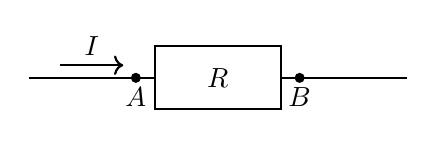
\begin{tikzpicture}[scale=0.8]

\draw[thick] (0,0) -- (2,0);
\draw[thick,->] (0.5,0.2) -- (1.5,0.2) node at (1,0.5) {$I$};
\node at (3,0) {$R$};
\filldraw (1.7,0) circle (2pt) node[below] (1.7,0) {$A$};
\filldraw (4.3,0) circle (2pt) node[below] (4.3,0) {$B$};

\draw[thick] (2,-0.5) rectangle (4,0.5);
\draw[thick] (4,0) -- (6,0);

\end{tikzpicture}



\begin{enumerate}[label=\Alph*)]
\item $-12$
\item 8
\item $-8$
\item 12
\item 3
\end{enumerate}

\item Uchlaridagi kuchlanish $24$ V, qarshiligi $20~\Omega$ bo‘lgan o‘tkazgichdan $60$ s vaqt ichida qancha (C) zaryad o‘tadi?
\begin{enumerate}[label=\Alph*)]
\item 17
\item 40
\item 24
\item 72
\item 25
\end{enumerate}

\item Quyida qarshiligi $12~\Omega$ bo‘lgan o‘tkazgichning uchlariga qo‘yilgan potensiallar farqining vaqtga bog‘liqligi ko‘rsatilgan. O‘tkazgichdan o‘tgan tok kuchini (A) aniqlang.

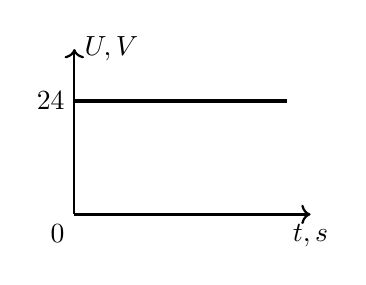
\begin{tikzpicture}[scale=0.6]
    % Koordinata o'qlari
    \draw[->, thick] (0,0) -- (5,0) node[below] { $t, s$}; % Vaqt o'qi
    \draw[->, thick] (0,0) -- (0,3.5) node[right] { $U, V$}; % Kuchlanish o'qi

    % Grafik chizig'i (O'zgarmas kuchlanish 24 V)
    % Masshtabni moslash uchun 2.4 birlik balandlikda chizamiz
    \draw[very thick] (0,2.4) -- (4.5,2.4);

    % Qiymatlarni belgilash
    \node[left] at (0,2.4) { $24$}; % Kuchlanish qiymati
    \node[below left] at (0,0) { $0$}; % Koordinata boshi

\end{tikzpicture}

\begin{enumerate}[label=\Alph*)]
\item 0
\item 0,5
\item 2
\item 1
\item 4
\end{enumerate}

\item Qarshiligi $12~\Omega$ bo‘lgan o‘tkazgichdan $3$ minutda $90$ C elektr miqdori o‘tgan. Bu o‘tkazgich uchlaridagi kuchlanishni toping (V).
\begin{enumerate}[label=\Alph*)]
\item 12
\item 6
\item 10
\item 9
\item 15
\end{enumerate}

\item Qarshiligi $2~\Omega$ bo‘lgan silindrsimon metall o‘tkazgich uchlariga $24$ V kuchlanish qo‘yilgan. Bu o‘tkazgich ko‘ndalang kesimidan $32$ s da nechta elektron o‘tadi?
\begin{enumerate}[label=\Alph*)]
\item $2,4\cdot10^{21}$
\item $2,4\cdot10^{20}$
\item $2,4\cdot10^{22}$
\item $2,4\cdot10^{19}$
\end{enumerate}

\item O‘zgarmas kuchlanish manbaiga ulangan reostatning surqichi surilib, qarshiligi $4$ marta kamaytirilsa, undagi tok kuchi qanday o‘zgaradi?
\begin{enumerate}[label=\Alph*)]
\item 2 marta ortadi.
\item 2 marta kamayadi.
\item 4 marta ortadi.
\item o‘zgarmaydi.
\item 4 marta kamayadi.
\end{enumerate}

\item Reostatdagi kuchlanish $2$ marta orttirildi, uning qarshiligi esa $3$ marta kamaytirildi. Reostatdagi tok qanday o‘zgaridi?
\begin{enumerate}[label=\Alph*)]
\item 1,5 marta kamaydi.
\item 1,5 marta ortdi.
\item o‘zgarmadi.
\item 6 marta kamaydi.
\item 6 marta ortdi.
\end{enumerate}

\item Elektr zanjirining o‘zgarmas qarshilikka ega bo‘lgan qismidan o‘tayotgan tok kuchi $4$ marta oshirilsa, shu qismdagi kuchlanish qanday o‘zgaradi?
\begin{enumerate}[label=\Alph*)]
\item 4 marta kamayadi.
\item 4 marta oshadi.
\item 2 marta kamayadi.
\item 2 marta oshadi.
\item o‘zgarmaydi.
\end{enumerate}

\item O‘tkazgich uchlaridagi kuchlanish ...
\begin{enumerate}[label=\Alph*)]
\item o‘tkazgichdan o‘tayotgan tok kuchi bilan o‘tkazgich qarshiligi ko‘paytmasiga teng.
\item o‘tkazgich ichida zaryadni ko‘chirishda bajarilgan ishga teng.
\item o‘tkazgich qarshiligini tok kuchiga nisbatiga teng.
\item o‘tkazgichdan o‘tayotgan tok kuchining o‘tkazgich qarshiligiga nisbatiga teng.
\item TJY.
\end{enumerate}

\item C/s birlik javobda keltirilgan birliklarning qaysi biriga teng kuchli?
\begin{enumerate}[label=\Alph*)]
\item V/$\Omega$
\item V/m
\item V
\item V$\cdot$m
\item V$\cdot\Omega$
\end{enumerate}

\item Quyidagilardan qaysi biri Xalqaro Birliklar Sistemasi (SI) dagi asosiy birlik hisoblanadi?
\begin{enumerate}[label=\Alph*)]
\item Volt
\item Kulon
\item Amper
\item Om
\item Farad
\end{enumerate}

\item Quyida keltirilgan birliklarning qaysilari kuchlanishning birligi bo‘la olmaydi?\\
1) A/s; \quad
2) J/C;\quad
3) A$\cdot$s$\Omega$;\quad
4) N/C;\quad
5) Nm/C;\quad
6) W/A;\quad
7) V.

\begin{enumerate}[label=\Alph*)]
\item 1, 2, 4
\item 1, 4
\item 1, 2, 3, 4, 5, 6
\item 1, 4, 6
\item 2, 3, 5, 6
\end{enumerate}

\item O‘lchamligi V$^2\cdot$s/J ko‘rinishida bo‘lgan fizik kattalikni ayting.
\begin{enumerate}[label=\Alph*)]
\item kuchlanish.
\item solishtirma qarshilik.
\item qarshilik.
\item zichlik.
\item tok kuchi.
\end{enumerate}

\item Rasmda to‘rtta har xil o‘tkazgichdagi tok kuchining kuchlanishga bog‘lanish grafiglari berilgan. O‘tkazgichlar qarshiliklari haqida nima deyish mumkin?

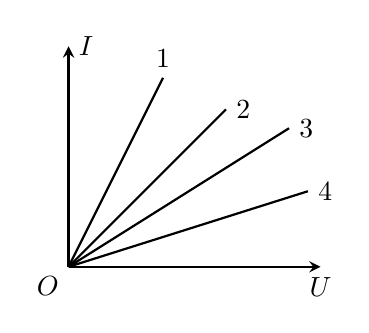
\begin{tikzpicture}[>=stealth, scale=0.8]
    % Koordinata o'qlari
    \draw[->, thick] (0,0) -- (4,0) node[below] {$U$}; % Kuchlanish o'qi
    \draw[->, thick] (0,0) -- (0,3.5) node[right] {$I$}; % Tok kuchi o'qi
    \node[below left] at (0,0) {$O$};

    % To'rtta o'tkazgichning grafik chiziqlari
    \draw[thick] (0,0) -- (1.5, 3) node[above] {1};
    \draw[thick] (0,0) -- (2.5, 2.5) node[right] {2};
    \draw[thick] (0,0) -- (3.5, 2.2) node[right] {3};
    \draw[thick] (0,0) -- (3.8, 1.2) node[right] {4};

\end{tikzpicture}

\begin{enumerate}[label=\Alph*)]
\item $R_1$ eng katta, $R_4$ eng kichik.
\item $R_4$ eng katta, $R_1$ eng kichik.
\item $R_1=R_2=R_3=R_4$.
\item $R_2>R_1>R_3>R_4$.
\item $R_1+R_2=R_3+R_4$.
\end{enumerate}

\item Rasmda uchta turli o‘tkazgich uchun tok kuchining kuchlanishga bog‘lanish grafiglari berilgan. Grafiklardan foydalanib, qaysi o‘tkazgichning qarshiligi eng katta ekanligini aniqlang.

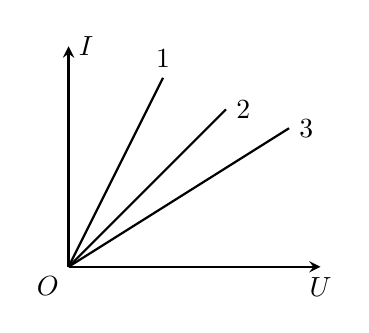
\begin{tikzpicture}[>=stealth, scale=0.8]
    % Koordinata o'qlari
    \draw[->, thick] (0,0) -- (4,0) node[below] {$U$}; % Kuchlanish o'qi
    \draw[->, thick] (0,0) -- (0,3.5) node[right] {$I$}; % Tok kuchi o'qi
    \node[below left] at (0,0) {$O$};

    % To'rtta o'tkazgichning grafik chiziqlari
    \draw[thick] (0,0) -- (1.5, 3) node[above] {1};
    \draw[thick] (0,0) -- (2.5, 2.5) node[right] {2};
    \draw[thick] (0,0) -- (3.5, 2.2) node[right] {3};
    

\end{tikzpicture}

\begin{enumerate}[label=\Alph*)]
\item 1
\item 2
\item 3
\item uchala o‘tkazgich qarshiligi bir xil.
\item TJY.
\end{enumerate}

\item O‘tkazgichdan o‘tayotgan tok kuchining kuchlanishga bog‘lanish grafigidan foydalanib, o‘tkazgichning qarshiligini hisoblang ($\Omega$).

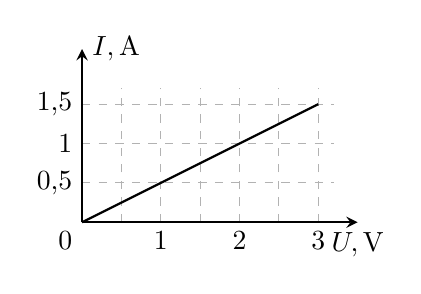
\begin{tikzpicture}[>=stealth, scale=1]
    % Punktir to'r (grid) chizish
    \draw[dashed, thin, gray!60, step=0.5] (0,0) grid (3.2, 1.7);

    % Koordinata o'qlari
    \draw[->, thick] (0,0) -- (3.5,0) node[below] {$U, \text{V}$}; % Kuchlanish o'qi
    \draw[->, thick] (0,0) -- (0,2.2) node[right] {$I, \text{A}$};   % Tok kuchi o'qi
    \node[below left] at (0,0) {0};

    % Grafik chizig'i (I = 0.5 * U bog'liqligi)
    % U=1 da I=0.5; U=2 da I=1; U=3 da I=1.5
    \draw[thick] (0,0) -- (3, 1.5); 

    % Gorizontal o'qdagi (U) qiymatlar
    \node[below] at (1,0) {1};
    \node[below] at (2,0) {2};
    \node[below] at (3,0) {3};

    % Vertikal o'qdagi (I) qiymatlar
    \node[left] at (0,0.5) {0,5};
    \node[left] at (0,1) {1};
    \node[left] at (0,1.5) {1,5};

\end{tikzpicture}

\begin{enumerate}[label=\Alph*)]
\item 0,5
\item 1
\item 1,5
\item 2
\item 4,5
\end{enumerate}

\item Grafikdan foydalanib, o‘tkazgichning qarshiligini toping ($\Omega$).

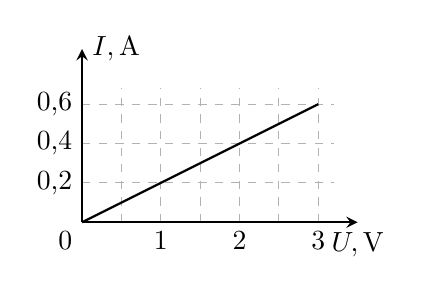
\begin{tikzpicture}[>=stealth, scale=1]
    % Punktir to'r (grid) chizish
    \draw[dashed, thin, gray!60, step=0.5] (0,0) grid (3.2, 1.7);

    % Koordinata o'qlari
    \draw[->, thick] (0,0) -- (3.5,0) node[below] {$U, \text{V}$}; % Kuchlanish o'qi
    \draw[->, thick] (0,0) -- (0,2.2) node[right] {$I, \text{A}$};   % Tok kuchi o'qi
    \node[below left] at (0,0) {0};

    % Grafik chizig'i (I = 0.5 * U bog'liqligi)
    % U=1 da I=0.5; U=2 da I=1; U=3 da I=1.5
    \draw[thick] (0,0) -- (3, 1.5); 

    % Gorizontal o'qdagi (U) qiymatlar
    \node[below] at (1,0) {1};
    \node[below] at (2,0) {2};
    \node[below] at (3,0) {3};

    % Vertikal o'qdagi (I) qiymatlar
    \node[left] at (0,0.5) {0,2};
    \node[left] at (0,1) {0,4};
    \node[left] at (0,1.5) {0,6};

\end{tikzpicture}

\begin{enumerate}[label=\Alph*)]
\item 0,2
\item 1,8
\item 5
\item 0,8
\item 3,6
\end{enumerate}

\item O‘tkazgichlarning volt–amper xarakteristikasidan foydalanib, 1-o‘tkazgich qarshiligining 2-o‘tkazgich qarshiligiga nisbatini toping.


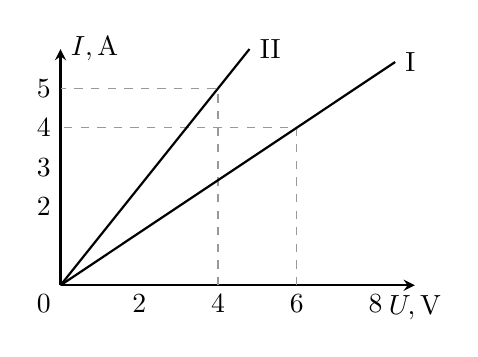
\begin{tikzpicture}[>=stealth, scale=0.5]
    % Koordinata o'qlari
    \draw[->, thick] (0,0) -- (9,0) node[below] {$U, \text{V}$}; % Kuchlanish o'qi
    \draw[->, thick] (0,0) -- (0,6) node[right] {$I, \text{A}$}; % Tok kuchi o'qi
    \node[below left] at (0,0) {0};

    % Nuqtalarni ko'rsatuvchi punktir chiziqlar
    \draw[dashed, gray!80] (4,0) -- (4,5) -- (0,5); % II-chiziq uchun nuqta (4; 5)
    \draw[dashed, gray!80] (6,0) -- (6,4) -- (0,4); % I-chiziq uchun nuqta (6; 4)

    % Grafik chiziqlari
    \draw[thick] (0,0) -- (4.8, 6) node[right] {II}; % II-o'tkazgich grafigi
    \draw[thick] (0,0) -- (8.5, 5.67) node[right] {I}; % I-o'tkazgich grafigi

    % Qiymatlarni belgilash (U o'qi)
    \node[below] at (2,0) {2};
    \node[below] at (4,0) {4};
    \node[below] at (6,0) {6};
    \node[below] at (8,0) {8};

    % Qiymatlarni belgilash (I o'qi)
    \node[left] at (0,2) {2};
    \node[left] at (0,3) {3};
    \node[left] at (0,4) {4};
    \node[left] at (0,5) {5};

\end{tikzpicture}

\begin{enumerate}[label=\Alph*)]
\item 2
\item 1,95
\item 1,78
\item 1,1
\item 1,875
\end{enumerate}

\item Chizmadan foydalanib, qarshilik $2,5~\Omega$ va $1~\Omega$ bo‘lgandagi toklarning nisbatini toping.

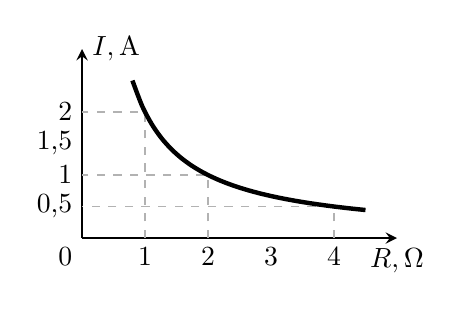
\begin{tikzpicture}[>=stealth, scale=0.8]
    % Koordinata o'qlari
    \draw[->, thick] (0,0) -- (5,0) node[below] {$R, \Omega$}; % Qarshilik o'qi
    \draw[->, thick] (0,0) -- (0,3) node[right] {$I, \text{A}$}; % Tok kuchi o'qi
    \node[below left] at (0,0) {0};

    % Nuqtalarni belgilash uchun punktir chiziqlar (Setka)
    \draw[dashed, gray!60] (1,0) -- (1,2) -- (0,2);
    \draw[dashed, gray!60] (2,0) -- (2,1) -- (0,1);
    \draw[dashed, gray!60] (4,0) -- (4,0.5) -- (0,0.5);

    % Grafik chizig'i (I = 2/R bog'liqligi)
    \draw[ultra thick, domain=0.8:4.5, smooth] plot (\x, {2/\x});

    % Qiymatlarni belgilash (R o'qi)
    \node[below] at (1,0) {1};
    \node[below] at (2,0) {2};
    \node[below] at (3,0) {3};
    \node[below] at (4,0) {4};

    % Qiymatlarni belgilash (I o'qi)
    \node[left] at (0,0.5) {0,5};
    \node[left] at (0,1) {1};
    \node[left] at (0,1.5) {1,5};
    \node[left] at (0,2) {2};

\end{tikzpicture}

\begin{enumerate}[label=\Alph*)]
\item 2,5
\item 0,3
\item 2
\item 0,4
\item 0,1
\end{enumerate}

\item O‘tkazgichning qarshiligi nimaga bog‘liq?
\begin{enumerate}[label=\Alph*)]
\item tok kuchiga.
\item kuchlanishga.
\item o‘tkazgich materiali va geometrik o‘lchamlariga.
\item tok zichligiga.
\item o‘tkazgichdagi tok kuchi va kuchlanishga.
\end{enumerate}

\item O‘tkazgich uchlaridagi kuchlanishni orttirsak, uning qarshiligi...
\begin{enumerate}[label=\Alph*)]
\item ortadi.
\item o‘zgarmaydi.
\item kamayadi.
\item ortishi ham, kamayishi ham mumkin.
\item TJY.
\end{enumerate}

\item Berilgan formulalardan qaysi biri o‘tkazgich qarshiligining uning uzunligiga bog‘lanishini ifodalaydi?
\begin{enumerate}[label=\Alph*)]
\item $R=R_0(1+\alpha t)$.
\item $R=\dfrac{U}{I}$.
\item $R=\rho\dfrac{l}{S}$.
\item $R=\dfrac{Q}{I^2t}$.
\item $R=\dfrac{P}{I^2}$.
\end{enumerate}

\item Cho‘g‘lanma lampaning spiralini yasash uchun uzunligi $40$ cm va ko‘ndalang kesim yuzi $0,002$ mm$^2$ bo‘lgan volfram sim olingan. Volframning solishtirma qarshiligi $5,5\cdot10^{-8}~\Omega\cdot$m. Spiralning qarshiligini toping ($\Omega$)?
\begin{enumerate}[label=\Alph*)]
\item 0,11
\item 1,1
\item 5,5
\item 11
\item 110
\end{enumerate}

\item Uzunligi $50$ m va ko‘ndalang kesim yuzi $34$ mm$^2$ bo‘lgan mis simning qarshiligini toping (m$\Omega$). Misning solishtirma qarshiligi $1,7\cdot10^{-8}~\Omega\cdot$m.
\begin{enumerate}[label=\Alph*)]
\item 25
\item 5
\item 50
\item 500
\item 5000
\end{enumerate}

\item Uzunligi $210$ m bo‘lgan nikelin simning qarshiligi $14,7~\Omega$ ga teng. Uning ko‘ndalang kesim yuzini toping (mm$^2$). $\rho=4,2\cdot10^{-7}~\Omega\cdot$m.
\begin{enumerate}[label=\Alph*)]
\item 1
\item 4
\item 1,5
\item 6
\item 4,5
\end{enumerate}

\item Ko‘ndalang kesim yuzi $0,5$ cm$^2$ bo‘lgan aluminiy simning qarshiligi $2,8~\Omega$ bo‘lsa. Simning uzunligini toping (m). $\rho=2,8\cdot10^{-8}~\Omega\cdot$m.
\begin{enumerate}[label=\Alph*)]
\item 1,4
\item 5
\item 50
\item 500
\item 5000
\end{enumerate}

\item Ko‘ndalang kesim yuzi $0,17$ mm$^2$ bo‘lgan mis simning qarshiligi $9~\Omega$ bo‘lishi uchun uzunligi necha metr bo‘lishi kerak? Misning solishtirma qarshiligi $1,7\cdot10^{-8}~\Omega\cdot$m.
\begin{enumerate}[label=\Alph*)]
\item 900
\item 90
\item 170
\item 200
\item 270
\end{enumerate}

\item Quyida keltirilgan mis simlarning qaysi biri eng katta qarshilikka ega?

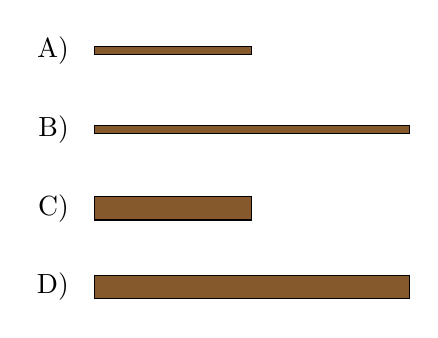
\begin{tikzpicture}
    % Sim A (O'rtacha uzunlik, ingichka)
    \node[left] at (-0.2, 3) {A)};
    \draw[fill=brown!70!black] (0, 2.95) rectangle (2, 3.05);

    % Sim B (Uzun, ingichka)
    \node[left] at (-0.2, 2) {B)};
    \draw[fill=brown!70!black] (0, 1.95) rectangle (4, 2.05);

    % Sim C (O'rtacha uzunlik, yo'g'on)
    \node[left] at (-0.2, 1) {C)};
    \draw[fill=brown!70!black] (0, 0.85) rectangle (2, 1.15);

    % Sim D (Uzun, yo'g'on)
    \node[left] at (-0.2, 0) {D)};
    \draw[fill=brown!70!black] (0, -0.15) rectangle (4, 0.15);
\end{tikzpicture}


\item $12$ mV kuchlanish ulangan uzunligi $10$ m va kesimi $2$ mm$^2$ bo‘lgan po‘lat simdagi tok kuchini aniqlang (mA). $\rho=12\cdot10^{-8}~\Omega\cdot$m.
\begin{enumerate}[label=\Alph*)]
\item 20
\item 17
\item 10
\item 0,2
\item 0,1
\end{enumerate}

\item Ko‘ndalang kesimi $150$ mm$^2$, solishtirma qarshiligi $2,8\cdot10^{-8}~\Omega\cdot$m bo‘lgan $150$ km uzunlikdagi simdan o‘zgarmas elektr toki uzatish liniyasi tortilgan. Agar tok kuchi $100$ A bo‘lsa, liniyadagi kuchlanish tushuvi necha Volt bo‘ladi?
\begin{enumerate}[label=\Alph*)]
\item 280
\item 5600
\item 2800
\item 560
\item 1400
\end{enumerate}

\item Uzunligi $500$ km, ko‘ndalang kesimi yuzi $10$ mm$^2$ bo‘lgan alyuminiy simdan $10$ mA tok o‘tayotgan bo‘lsa, uning uchlaridagi kuchlanish necha Volt? Alyuminiyning solishtirma qarshiligi $2,8\cdot10^{-8}~\Omega\cdot$m.
\begin{enumerate}[label=\Alph*)]
\item 56
\item 50
\item 35
\item 28
\item 14
\end{enumerate}

\item Ko‘ndalang kesimi $1$ mm$^2$ bo‘lgan nikelin simdan yasalgan reostatga ulangan ampermetr $20$ A ni, voltmetr esa $210$ V ni ko‘rsatadi ($\rho=4,2\cdot10^{-7}~\Omega\cdot$m). Reostat simining uzunligi necha metr?
\begin{enumerate}[label=\Alph*)]
\item 150
\item 180
\item 200
\item 250
\item 300
\end{enumerate}

\item O‘tkazgichning kesim yuzi $2$ marta, uzunligi esa $3$ marta oshsa, uning qarshiligi qanday o‘zgaradi?
\begin{enumerate}[label=\Alph*)]
\item 3 marta kamayadi.
\item 1,5 marta ortadi.
\item 3 marta ortadi.
\item 1,5 marta kamayadi.
\item o‘zgarmaydi.
\end{enumerate}

\item Mis simning qarshiligi $6~\Omega$. Shu simdan ko‘ndalang kesimi yuzi $3$ marta, uzunligi esa $2$ marta katta bo‘lgan mis simning qarshiligi qanday ($\Omega$)?
\begin{enumerate}[label=\Alph*)]
\item 3
\item 4
\item 8
\item 9
\item 10
\end{enumerate}

\item Mis simning elektr qarshiligi $6~\Omega$ ga teng. Uzunligi $3$ marta, diametri $2$ marta katta bo‘lgan mis simning qarshiligi qanday ($\Omega$)?
\begin{enumerate}[label=\Alph*)]
\item 72
\item 9
\item 8
\item 4
\item 4,5
\end{enumerate}

\item Mis simning elektr qarshiligi $6~\Omega$ ga teng. Uzunligi $3$ marta, diametri $2$ marta kichik bo‘lgan mis simning qarshiligi qanday ($\Omega$)?
\begin{enumerate}[label=\Alph*)]
\item 72
\item 9
\item 8
\item 4,5
\item 4
\end{enumerate}

\item Uzunligi $l$, ko‘ndalang kesim yuzi $S$ bo‘lgan o‘tkazgich $4~\Omega$ elektr qarshilikka ega. Xuddi moddadan yasalgan, uzunligi $2l$, ko‘ndalang kesimi $S/4$ bo‘lgan o‘tkazgich necha qarshilikka ega bo‘ladi?
\begin{enumerate}[label=\Alph*)]
\item 32
\item 16
\item 8
\item 24
\item 4
\end{enumerate}

\item Birinchi o‘tkazgichning uzunligi $1$ m, ko‘ndalang kesim yuzi $1$ mm$^2$, ikkinchi o‘tkazgichning uzunligi $2$ m, ko‘ndalang kesim yuzi $0,5$ mm$^2$. Bu o‘tkazgichlarning qarshiliklari $R_1$ va $R_2$ qanday munosabatda bo‘ladi?
\begin{enumerate}[label=\Alph*)]
\item $R_1=R_2$.
\item $R_1=4R_2$
\item aniqlab bo‘lmaydi.
\item $R_2=2R_1$
\item $R_2=4R_1$
\end{enumerate}

\item Alyuminiydan yasalgan bir xil uzunlikdagi ikki simdan birining qarshiligi $2,7~\Omega$, ikkinchisiniki $1,8~\Omega$. Birinchi simning ko‘ndalang kesim yuzi $4$ mm$^2$. Ikkinchi simning ko‘ndalang kesim yuzi qanday (mm$^2$)?
\begin{enumerate}[label=\Alph*)]
\item 9
\item 18
\item 12
\item 6
\item 3
\end{enumerate}

\item Uzunliklari bir xil, ko‘ndalang kesimlari $S_1=2S_2$ va solishtirma qarshiliklari $\rho_2=2\rho_1$ bo‘lgan ikkita o‘tkazgich qarshiliklarining nisbati $R_2/R_1$ ni aniqlang.
\begin{enumerate}[label=\Alph*)]
\item 0,25
\item 0,5
\item 2
\item 4
\item 8
\end{enumerate}

\item Uzunligi $1$ m va ko‘ndalang kesim yuzi $0,5$ mm$^2$ bo‘lgan o‘tkazgichning qarshiligi teng qarshilik hosil qilish uchun, o‘sha materialdan yasalgan va ko‘ndalang kesim yuzi $10$ mm$^2$ bo‘lgan simdan necha metr olish kerak?
\begin{enumerate}[label=\Alph*)]
\item 10
\item 20
\item 30
\item 40
\item 50
\end{enumerate}

\item Ko‘ndalang kesim yuzi $1$ mm$^2$ va og‘irligi $105$ N bo‘lgan kumush simning qarshiligini toping ($\Omega$)? Kumushning zichligi $10500$ kg/m$^3$, solishtirma qarshiligi $1,6\cdot10^{-8}~\Omega\cdot$m.
\begin{enumerate}[label=\Alph*)]
\item 16
\item 8
\item 32
\item 40
\item 48
\end{enumerate}

\item Agar o‘tkazgich uchlaridagi kuchlanish $2$ marta kamaytirilsa va uning uzunligi $2$ marta orttirilsa, undan o‘tayotgan tok kuchi qanday o‘zgaradi?
\begin{enumerate}[label=\Alph*)]
\item o‘zgarmaydi.
\item 4 marta kamayadi.
\item 4 marta ortadi.
\item 2 marta ortadi.
\item 2 marta ortadi.
\end{enumerate}

\item Bir simning uzunligi $20$ cm, ikkinchisiniki $1,6$ m. Simlarning ko‘ndalang kesimi va materiallari bir xil. Qaysi simning qarshiligi katta va necha marta katta?
\begin{enumerate}[label=\Alph*)]
\item birinchisiniki, 3,2 marta.
\item ikkinchisiniki, 3,2 marta.
\item bir xil.
\item birinchisiniki, 8 marta.
\item ikkinchisiniki, 8 marta.
\end{enumerate}

\item Agar metall simning uzunligi va radiusi $4$ marta orttirilsa, uning qarshiligi qanday o‘zgaradi?
\begin{enumerate}[label=\Alph*)]
\item 4 marta kamayadi.
\item 2 marta ortadi.
\item o‘zgarmaydi.
\item 2 marta kamayadi.
\item 4 marta ortadi.
\end{enumerate}

\item Simni cho‘zib, $3$ marta uzaytirilsa, qarshiligi necha marta ortadi?
\begin{enumerate}[label=\Alph*)]
\item 9
\item 4
\item 2
\item 3
\item o‘zgarmaydi.
\end{enumerate}

\item Manbaning kuchlanishi $2$ marta orttirilsa, rezistor qarshiligi qanday o‘zgaridi?
\begin{enumerate}[label=\Alph*)]
\item 2 marta ortadi.
\item 2 marta kamayadi.
\item 4 marta ortadi.
\item o‘zgarmaydi.
\item 4 marta kamayadi.
\end{enumerate}

\item Zanjirdagi tok kuchi $5$ marta orttirilsa, rezistorning qarshiligi qanday o‘zgaradi?
\begin{enumerate}[label=\Alph*)]
\item 5 marta ortadi.
\item 5 marta kamayadi.
\item 25 marta ortadi.
\item o‘zgarmaydi.
\item 25 marta kamayadi.
\end{enumerate}

\item Massalari teng bo‘lgan sim teng ikkita metallikdan ikkita sim tayyorlandi. Ulardan biri ikkinchisidan $3$ marta uzun. Bu simlarning qarshiliklari $R_1$ va $R_2$ orasidagi munosabatni aniqlang.
\begin{enumerate}[label=\Alph*)]
\item $R_1=3R_2$
\item $R_2=9R_1$
\item $R_1=R_2$
\item $R_1=9R_2$
\item $R_2=3R_1$
\end{enumerate}

\item Birinchisining diametri ikkinchisinikidan $2$ marta katta bo‘lgan ikkita temir o‘tkazgich bir xil og‘irlikka ega. Bu o‘tkazgichlarning qarshiliklarini taqqoslang.
\begin{enumerate}[label=\Alph*)]
\item birinchisiniki 2 marta katta.
\item birinchisiniki 4 marta katta.
\item ikkinchisiniki 4 marta katta.
\item birinchisiniki 2 marta katta.
\item TJY.
\end{enumerate}

\item $8,9$ kg massali ko‘ndalang kesim yuzi $1$ mm$^2$ bo‘lgan mis simning qarshiligini necha $\Omega$ bo‘ladi? Misning zichligi $8,9$ g/cm$^3$, solishtirma qarshiligi $1,7\cdot10^{-8}~\Omega\cdot$m.
\begin{enumerate}[label=\Alph*)]
\item 8,9
\item 17
\item 34
\item 44,5
\item 51
\end{enumerate}

\item Har bir metr uzunligining massasi $3,9$ kg bo‘lgan $1$ km uzunlikdagi po‘lat relsning qarshiligini aniqlang ($\Omega$). Po‘latning zichligi $7800$ kg/m$^3$, solishtirma qarshiligi $1,2\cdot10^{-7}~\Omega\cdot$m.
\begin{enumerate}[label=\Alph*)]
\item 0,17
\item 0,3
\item 0,18
\item 0,55
\item 0,24
\end{enumerate}

\item Har $1$ metrining massasi $78$ kg bo‘lgan po‘lat relsning har bir metri $0,012~\Omega$ qarshilikka ega bo‘ladi? Po‘latning zichligi $7,8$ g/cm$^3$, solishtirma qarshiligi $1,2\cdot10^{-7}~\Omega\cdot$m.
\begin{enumerate}[label=\Alph*)]
\item 1200
\item 1000
\item 100
\item 780
\item 10
\end{enumerate}

\item Uzunligi $l$, qarshiligi $R$ va solishtirma qarshiligi $\rho$ bo‘lgan o‘tkazgichning hajmini toping.
\begin{enumerate}[label=\Alph*)]
\item $\rho R l^2$
\item $\dfrac{l^2}{\rho R}$
\item $\dfrac{\rho l^2}{R}$
\item $\dfrac{\rho l^2}{R}$
\item $\dfrac{Rl^2}{\rho}$
\end{enumerate}

\item Uzunligi $l$, qarshiligi $R$, zichligi $d$ va solishtirma qarshiligi $\rho$ bo‘lgan o‘tkazgich massasi qanday?
\begin{enumerate}[label=\Alph*)]
\item $\dfrac{R}{\rho d l^2}$
\item $\dfrac{\rho l^2}{dR}$
\item $\dfrac{d\rho l^2}{R}$
\item $\dfrac{Rl^2}{\rho d}$
\item $\dfrac{d\rho}{Rl^2}$
\end{enumerate}

\item Uzunligi $1$ km bo‘lgan mis simning qarshiligi $75,65~\Omega$. Simning og‘irligi necha Nyuton? Misning zichligi $8900$ kg/m$^3$, solishtirma qarshiligi $1,7\cdot10^{-8}~\Omega\cdot$m.
\begin{enumerate}[label=\Alph*)]
\item 225
\item 45
\item 83
\item 18
\item 20
\end{enumerate}

\item Elektr spiralidan $6$ A tok o‘tmoqda. Agar spiralning chorak qismi kesib tashlansa, undan necha Amper tok o‘tadi? $U=\text{const}$.
\begin{enumerate}[label=\Alph*)]
\item 12
\item 10
\item 4,5
\item 8
\item 18
\end{enumerate}

\item Bir simni teng ikki bo‘lakka bo‘lib, ikkala bo‘lagi ustma-ust taxlansa, simning qarshiligi qanday o‘zgaradi?
\begin{enumerate}[label=\Alph*)]
\item o‘zgarmaydi.
\item 4 marta oshadi.
\item 2 marta kamayadi.
\item 2 marta oshadi.
\item 4 marta kamayadi.
\end{enumerate}

\item Uzun o‘tkazgich teng ikki bo‘lakka bo‘lindi va bitta o‘tkazgich tarzida uzunligi bo‘yicha eshib qo‘yildi. Bunda o‘tkazgichning qarshiligi qanday o‘zgaradi?
\begin{enumerate}[label=\Alph*)]
\item o‘zgarmaydi.
\item 4 marta ortadi.
\item 2 marta ortadi.
\item 4 marta kamayadi.
\item 2 marta kamayadi.
\end{enumerate}

\item Qarshiligi $R$ bo‘lgan sim teng uch qismga qirqildi va uchala qism uzunligi bo‘yicha birga eshib qo‘yildi. Bunda simning qarshiligi qanday bo‘ladi?
\begin{enumerate}[label=\Alph*)]
\item $9R$
\item $R$
\item $R/3$
\item $R/6$
\item $R/9$
\end{enumerate}


\item O‘tkazgich 5 ta bo‘lakka bo‘linib, zich qilib eshilganda, qarshiligi $1~\Omega$ bo‘ldi. O‘tkazgichning dastlabki qarshiligini toping ($\Omega$).
\begin{enumerate}[label=\Alph*)]
\item 5
\item 10
\item 15
\item 20
\item 25
\end{enumerate}

\item Qarshiligi $R$ bo‘lgan sim to‘rtta teng qismga qirqildi va to‘rttala qism uzunligi bo‘yicha birga eshib qo‘yildi. Bunday simning qarshiligi qanday bo‘ladi?
\begin{enumerate}[label=\Alph*)]
\item $R/32$
\item $R/12$
\item $R/16$
\item $R/4$
\item $R/2$
\end{enumerate}

\item Agar o‘tkazgichni (izolyatsiyasiz) ikki buksak va eshsak, qarshiligi qanday o‘zgaradi?
\begin{enumerate}[label=\Alph*)]
\item 2 marta ortadi.
\item 2 marta kamayadi.
\item 4 marta ortadi.
\item 4 marta kamayadi.
\item o‘zgarmaydi.
\end{enumerate}

\item Metall simning solishtirma qarshiligi $\rho$, uning ko‘ndalang kesim yuzi $S$ va undan o‘tayotgan tok kuchi $I$ bo‘lsa, sim ichidagi elektr maydon kuchlanganligi qanday bo‘ladi?
\begin{enumerate}[label=\Alph*)]
\item $E=\dfrac{I\rho S}{ }$
\item $E=\dfrac{I}{\rho S}$
\item $E=\dfrac{I^2\rho}{S}$
\item $E=\dfrac{IS}{\rho}$
\item $E=\dfrac{I\rho}{S}$
\end{enumerate}

\item $20$ A o‘zgarmas tok o‘tayotgan, ko‘ndalang kesim yuzi $1$ mm$^2$ bo‘lgan mis sim ichidagi elektr maydon kuchlanganligi qanday (V/m)? Misning solishtirma qarshiligi $1,7\cdot10^{-8}~\Omega\cdot$m.
\begin{enumerate}[label=\Alph*)]
\item 0,17
\item 0,34
\item 1,7
\item 3,4
\item 17
\end{enumerate}

\item Aluminiy o‘tkazgichdan o‘tayotgan tok zichligi $2\cdot10^6$ A/m$^2$ bo‘lsa, o‘tkazgich ichidagi maydon kuchlanganligi necha V/m bo‘ladi? Aluminiyning solishtirma qarshiligi $2\cdot10^{-8}~\Omega\cdot$m.
\begin{enumerate}[label=\Alph*)]
\item $10^{-2}$
\item $4\cdot10^{-3}$
\item 0
\item $4\cdot10^{-4}$
\item $4\cdot10^{-2}$
\end{enumerate}

\item Uzunligi $10$ m, solishtirma qarshiligi $5\cdot10^{-7}~\Omega\cdot$m bo‘lgan o‘tkazgichga $10$ V kuchlanish berilgan. O‘tkazgichdagi tokning zichligi nimaga teng (A/m$^2$)?
\begin{enumerate}[label=\Alph*)]
\item $10^3$
\item $10^4$
\item $2\cdot10^4$
\item $2\cdot10^6$
\item $2\cdot10^7$
\end{enumerate}

\item Uzunligi $2$ m bo‘lgan nixrom simdagi kuchlanish tushishi $2,5$ V bo‘lsa, undagi tok zichligi necha A/m$^2$ ga teng? Nixromning solishtirma qarshiligi $1\cdot10^{-6}~\Omega\cdot$m.
\begin{enumerate}[label=\Alph*)]
\item $2\cdot10^3$
\item $2,4\cdot10^4$
\item $10^5$
\item $1,25\cdot10^6$
\item 100
\end{enumerate}

\item Mis simdan o‘tayotgan tokning zichligi $1$ A/mm$^2$ ga teng. Simdagi elektr maydon kuchlanganligi qanday (V/m)? Misning solishtirma qarshiligi $1,7\cdot10^{-8}~\Omega\cdot$m.
\begin{enumerate}[label=\Alph*)]
\item 34
\item 17
\item 3,4
\item 1,7
\item 0,017
\end{enumerate}

\item Bir xil materialdan tayyorlangan, bir xil uzunlikdagi ikkita o‘tkazgich ko‘ndalang kesimlarining nisbati $S_1/S_2=2$. Shu o‘tkazgichlarga bir xil kuchlanish berilganda, ulardagi tok zichliklari qanday munosabatda bo‘ladi?
\begin{enumerate}[label=\Alph*)]
\item $j_1=j_2$
\item $j_1=0,25j_2$
\item $j_1=j_2$
\item $j_1=4j_2$
\item $j_1=0,5j_2$
\end{enumerate}

\item Uzunliklarining nisbati $l_2/l_1=2$, ko‘ndalang kesimlarining nisbati $S_2/S_1=2$ bo‘lgan, bir xil materialdan tayyorlangan ikkita o‘tkazgichga bir xil kuchlanish berilsa, ulardagi tok zichliklari qanday munosabatda bo‘ladi?
\begin{enumerate}[label=\Alph*)]
\item $j_2=2j_1$
\item $j_1=4j_2$
\item $j_1=j_2$
\item $j_1=2j_2$
\item $j_2=4j_1$
\end{enumerate}

\item O‘tkazgich uzunligini va unga qo‘yilgan potensial ayirmani o‘zgartirmagan holda ko‘ndalang kesim yuzini $2$ marta kamaytirsak, undagi tok zichligi qanday o‘zgaradi?
\begin{enumerate}[label=\Alph*)]
\item o‘zgarmaydi.
\item 4 marta kamayadi.
\item 4 marta ortadi.
\item 2 marta kamayadi.
\item 2 marta ortadi.
\end{enumerate}

\item O‘tkazgichning ko‘ndalang kesim yuzi va unga qo‘yilgan potensiallar ayirmasini o‘zgartirmagan holda uzunligini $2$ marta kamaytirsak, undagi tok zichligi qanday o‘zgaradi?
\begin{enumerate}[label=\Alph*)]
\item o‘zgarmaydi.
\item 4 marta ortadi.
\item 4 marta ortadi.
\item 2 marta ortadi.
\item 2 marta kamayadi.
\end{enumerate}

\item Metall simdagi elektr maydon kuchlanganligi $8$ marta kamaysa va simning kesim yuzi $10$ marta ortsa, undagi tok kuchi qanday o‘zgaradi?
\begin{enumerate}[label=\Alph*)]
\item $1,25$ marta kamayadi.
\item 8 marta ortadi.
\item 4 marta kamayadi.
\item $1,25$ marta ortadi.
\item TJY.
\end{enumerate}



\begin{table}[h!]
\centering
\begin{tabular}{|c|c|c|c|c|c|c|c|c|c|}
\hline
1b & 2b & 3d & 4e & 5a & 6c & 7d & 8c & 9a & 10d \\ \hline
11c & 12b & 13a & 14c & 15e & 16b & 17a & 18a & 19c & 20b \\ \hline
21c & 22b & 23c & 24d & 25c & 26e & 27d & 28c & 29b & 30c \\ \hline
31d & 32a & 33d & 34e & 35b & 36b & 37a & 38c & 39e & 40d \\ \hline
41b & 42b & 43e & 44c & 45a & 46e & 47d & 48d & 49b & 50a \\ \hline
51b & 52e & 53c & 54a & 55d & 56d & 57d & 58e & 59b & 60e \\ \hline
61d & 62c & 63c & 64e & 65d & 66d & 67d & 68e & 69e & 70c \\ \hline
71d & 72e & 73b & 74e & 75d & 76d & 77e & 78c & 79d & 80a \\ \hline
81d & 82d &  &  &  &  &  &  &  &  \\ \hline
\end{tabular}
\end{table}





\end{enumerate}
\section{Qarshiliklarni hisoblash}


\begin{enumerate}

\item Qarshiliklari $3~\Omega$ va $4~\Omega$ bo‘lgan o‘tkazgichlar ketma-ket ulangan. Umumiy qarshilikni toping ($\Omega$). 
\begin{enumerate}[label=\Alph*)]
\item 12/7
\item 7
\item 1
\item 12
\end{enumerate}

\item Qarshiliklari $12~\Omega, 5~\Omega$ va $14~\Omega$ bo‘lgan o‘tkazgichlar ketma-ket ulangan. Umumiy qarshilikni toping ($\Omega$).
\begin{enumerate}[label=\Alph*)]
\item 24
\item 46
\item 38
\item 31
\end{enumerate}

\item Qarshiliklari $25~\Omega, 40~\Omega$ va $R_3$ bo‘lgan o‘tkazgichlar ketma-ket ulangan. Agar umumiy qarshilik $70~\Omega$ ga teng bo‘lsa, $R_3$ qiymatini toping ($\Omega$).
\begin{enumerate}[label=\Alph*)]
\item 8
\item 9
\item 2
\item 5
\end{enumerate}

\item Har birining qarshiligi $4~\Omega$ dan bo‘lgan $13$ ta bir xil qarshilik ketma-ket ulangan. Umumiy qarshilikni toping ($\Omega$). 
\begin{enumerate}[label=\Alph*)]
\item 4/13
\item 17
\item 9
\item 52
\end{enumerate}

\item Qarshiliklari $1~\Omega$ va $3~\Omega$ bo‘lgan o‘tkazgichlar parallel ulangan. Umumiy qarshilikni toping ($\Omega$). 
\begin{enumerate}[label=\Alph*)]
\item 2
\item 4
\item 0,75
\item 4/3
\end{enumerate}

\item Qarshiliklari $R_1$ va $7~\Omega$ bo‘lgan o‘tkazgichlar parallel ulangan. Agar umumiy qarshilik $4,55~\Omega$ ga teng bo‘lsa, $R_1$ qiymatini toping ($\Omega$). 
\begin{enumerate}[label=\Alph*)]
\item 13
\item 2,45
\item 11,55
\item 5,89
\end{enumerate}

\item Elektr qarshiliklari $4~\Omega, 6~\Omega, 12~\Omega$ bo‘lgan uchta rezistor bir-biriga parallel ulangan. Umumiy qarshilik necha $\Omega$? 
\begin{enumerate}[label=\Alph*)]
\item 22
\item 11
\item 22/3
\item 2
\end{enumerate}

\item Ketma-ket ulangan ikkita bir xil o‘tkazgich parallel ulansa, umumiy qarshilik qanday o‘zgaradi? 
\begin{enumerate}[label=\Alph*)]
\item 2 marta kamayadi
\item 4 marta ortadi
\item 4 marta kamayadi
\item 2 marta ortadi
\end{enumerate}

\item Ikkita o‘tkazgich o‘zaro ketma-ket ulanganda, ularning umumiy qarshiligi $5~\Omega$, parallel ulanganda esa $1,2~\Omega$ bo‘ladi. O‘tkazgichlar qarshiliklarining nisbatini aniqlang.
\begin{enumerate}[label=\Alph*)]
\item 2
\item 1,5
\item 1
\item 0,75
\end{enumerate}

\item Zanjirga $n$ ta bir xil qarshiliklar parallel ulangan edi. Agar ular ketma-ket ulansa, zanjirning umumiy qarshiligi qanday o‘zgaradi? 
\begin{enumerate}[label=\Alph*)]
\item $n$ marta ortadi
\item $n^2$ marta kamayadi
\item $n$ marta kamayadi
\item $n^2$ marta ortadi
\end{enumerate}

\item Agar rasmda tasvirlangan zanjirda $R_1=2~\Omega, R_2=R_3=3~\Omega$ bo‘lsa, zanjirning AB oraliqdagi qarshiligi qanday ($\Omega$) bo‘ladi?

\begin{circuitikz} 
\draw
  (0,0) node[left] {A} to[short, o-] (0.5,0)
  to[R=$R_1$] (2.5,0) -- (3,0)
  (3,0.7) -- (3,-0.7)
  (3,0.7) to[R=$R_2$] (5,0.7) -- (5,0)
  (3,-0.7) to[R=$R_3$] (5,-0.7) -- (5,0)
  (5,0) to[short, -o] (5.5,0) node[right] {B};
\end{circuitikz}

\begin{enumerate}[label=\Alph*)]
\item 0,27
\item 3,5
\item 4
\item 7
\end{enumerate}

\item Rasmda tasvirlangan zanjirning umumiy qarshiligi necha $\Omega$? $R_1=3~\Omega, R_2=R_3=R_4=12~\Omega, R_5=5~\Omega$.

\begin{circuitikz}
\draw
  (0,0) to[R=$R_1$] (2,0) -- (2.5,0)
  (2.5,1) -- (2.5,-1)
  (2.5,1) to[R=$R_2$] (4.5,1) -- (4.5,0)
  (2.5,0) to[R=$R_3$] (4.5,0)
  (2.5,-1) to[R=$R_4$] (4.5,-1) -- (4.5,0)
  (4.5,0) -- (5,0) to[R=$R_5$] (7,0);
\end{circuitikz}

\begin{enumerate}[label=\Alph*)]
\item 20
\item 15
\item 5
\item 12
\end{enumerate}

\item Rasmda tasvirlangan zanjirning umumiy qarshiligi necha $\Omega$? $R_1=1~\Omega; R_2=R_3=2~\Omega; R_4=R_5=3~\Omega; R_6=4~\Omega$.

\begin{circuitikz}[european]
\draw
  % Chap tomondagi kirish va R1 rezistori
  (0,0) to[short, o-] (0.5,0)
  to[R=$R_1$] (2.5,0) -- (3,0)
  
  % Parallel blokning chap tomonidagi vertikal chiziq
  (3,1.5) -- (3,-1.5)
  
  % To'rtta parallel rezistor (R2, R3, R4, R5)
  (3,1.5) to[R=$R_2$] (5,1.5) -- (5,0)
  (3,0.5) to[R=$R_3$] (5,0.5) -- (5,0)
  (3,-0.5) to[R=$R_4$] (5,-0.5) -- (5,0)
  (3,-1.5) to[R=$R_5$] (5,-1.5) -- (5,0)
  
  % O'ng tomondagi R6 rezistori va chiqish
  (5,0) to[R=$R_6$] (7,0)
  to[short, -o] (7.5,0);
\end{circuitikz}

\begin{enumerate}[label=\Alph*)]
\item 5,6
\item 15
\item 10,5
\item 6,5
\end{enumerate}

\item Rasmda tasvirlangan zanjirning A va B nuqtalari orasidagi qarshilikni toping ($\Omega$). $R=2~\Omega$. 

\begin{circuitikz}[european]
\draw
  % Kvadratning asosi va rezistorlari
  (0,0) node[anchor=north] {A} 
  to[R=$R$, *-] (0,3)           % Chap tomon
  to[R=$R$] (3,3)                % Yuqori tomon
  to[R=$R$] (3,0)                % O'ng tomon
  node[anchor=north] {B}
  to[R=$R$, -*] (0,0);           % Pastki tomon (A va B orasida)

  % Diagonal rezistor (A nuqtasidan yuqori-o'ng burchakka)
\draw
  (0,0) to[R=$R$, *-] (3,3);
\end{circuitikz}

\begin{enumerate}[label=\Alph*)]
\item 1,6
\item 2,75
\item 2
\item 1,25
\end{enumerate}

\item Sxemasi rasmda berilgan zanjirning 1- va 4- nuqtalari orasidagi qarshiligini hisoblang.

\begin{circuitikz}[european]
\draw
  % Kvadratning burchaklari va yon tomonlaridagi rezistorlar
  (0,0) node[below left] {1} 
  to[R=$R$, *-*] (0,3) node[above left] {2}    % 1 va 2 orasida
  to[R=$R$, *-*] (3,3) node[above right] {3}   % 2 va 3 orasida
  to[R=$R$, *-*] (3,0) node[below right] {4}   % 3 va 4 orasida
  to[R=$R$, *-*] (0,0);                         % 4 va 1 orasida

  % Diagonal rezistor (1- va 3-nuqtalar orasida)
\draw
  (0,0) to[R=$2R$, *-*] (3,3);
\end{circuitikz}


\begin{enumerate}[label=\Alph*)]
\item 5R/3
\item 6R
\item 3R/2
\item 2R/3
\end{enumerate}

\item Rasmda tasvirlangan elektr zanjirning umumiy qarshiligini toping. 

\begin{circuitikz}[european]
\draw
  % Pastki asosiy sim va terminallar
  (0,0) to[short, o-o] (6,0)
  
  % Birinchi uchta parallel rezistorlar bloki
  (1,0) to[R=R, *-*] (1,2)
  (2,0) to[R=R, *-*] (2,2)
  (3,0) to[R=R, *-*] (3,2)
  
  % Yuqori tutashtiruvchi sim va gorizontal rezistor
  (1,2) -- (3,2)
  (3,2) to[R=R, -*] (5,2)
  
  % To'rtinchi (o'ng tarafdagi) vertikal rezistor
  (5,2) to[R=R, -*] (5,0);
\end{circuitikz}

\begin{enumerate}[label=\Alph*)]
\item 2R/3
\item R
\item 3R/4
\item 4R/3
\end{enumerate}

\item Rasmda tasvirlangan elektr zanjirning A va B nuqtalari orasidagi qarshilik necha $\Omega$? Rezistorlardan har birining qarshiligi $30~\Omega$ ga teng.

\begin{circuitikz}[european]
\draw
  (0,2) node[left] {A} to[short, o-*] (0.5,2)
  (0.5,2) -- (0.5,0) 
  (0.5,2) to[R=30$\Omega$] (3,2) 
  (3,2) to[R=30$\Omega$, *-*] (3,0)
  (0.5,0) -- (3,0)
  (3,2) -- (5.5,2) -- (5.5,0)
  (3,0) to[R=30$\Omega$] (5.5,0)
  (5.5,0) to[short, *-o] (6,0) node[right] {B};
\end{circuitikz}

\begin{enumerate}[label=\Alph*)]
\item 30
\item 20
\item 10
\item 45
\end{enumerate}

\item Har birining qarshiligi $3~\Omega$ dan bo‘lgan qarshiliklar rasmda ko‘rsatilgandek ulangan bo‘lsa, A va B nuqtalar orasidagi umumiy qarshilik necha $\Omega$?

\begin{circuitikz}[european]
\draw
  % Asosiy gorizontal chiziq va rezistorlar
  (0,0) node[left] {A} to[short, o-*] (0.5,0)
  (0.5,0) to[R] (2.5,0) coordinate (n1) % 1-rezistor
  to[R] (4.5,0) coordinate (n2)         % 2-rezistor
  to[R] (6.5,0)                         % 3-rezistor
  to[short, *-o] (7,0) node[right] {B};

  % Yuqoridagi sakrash simi: A nuqtasidan 2- va 3-rezistor orasiga
  \draw (0.5,0) -- (0.5,1) -- (4.5,1) to[short, -*] (n2);

  % Pastdagi sakrash simi: 1- va 2-rezistor orasidan B nuqtasiga
  \draw (2.5,0) to[short, *-] (2.5,-1) -- (6.5,-1) -- (6.5,0);
\end{circuitikz}

\begin{enumerate}[label=\Alph*)]
\item 0,5
\item 1
\item 3
\item 6
\end{enumerate}

\item B va C nuqtalari orasidagi umumiy qarshilikni ($\Omega$) toping. $R=2~\Omega$.

\begin{circuitikz}[european]
\draw
  % Asosiy aylana konturi (simlarni ifodalash uchun)
  (0,0) circle (2)
  
  % Markaziy vertikal qarshilik (R)
  % Bu rezistor aylananing yuqori va pastki nuqtalarini tutashtiradi
  (0,2) to[R=R, *-*] (0,-2)
  
  % Chap tarafdagi rezistorlar (B terminali tomonda)
  % Yuqori-chap va pastki-chap choraklardagi rezistorlar
  (0,2) to[R=R] (-2,0) 
  (-2,0) to[R=R] (0,-2)
  
  % O'ng tarafdagi rezistorlar (C terminali tomonda)
  % Yuqori-o'ng va pastki-o'ng choraklardagi rezistorlar
  (0,2) to[R=R] (2,0) 
  (2,0) to[R=R] (0,-2)
  
  % Terminal B (chapda) ulanishi
  (-2,0) to[short, *-o] (-2.8,0) node[left] {B}
  
  % Terminal C (o'ngda) ulanishi
  (2,0) to[short, *-o] (2.8,0) node[right] {C};
\end{circuitikz} chizmada xato bor

\begin{enumerate}[label=\Alph*)]
\item 0,6
\item 1,2
\item 0,8
\item 1
\end{enumerate}

\item $A_1$ ampermetr $2,5$ A, $A_2$ ampermetr $5$ A tokni ko‘rsatmoqda. Agar $R_1=4~\Omega$ bo‘lsa, $R_2$ qarshilik necha $\Omega$ bo‘ladi?

\begin{circuitikz}[european]
\draw
  % Kirish toki I
  (0,0) to[short, i=I, o-] (1,0) -- (1,0.8)
  
  % Yuqori tarmoq: A1 ampermetr va R1 rezistor
  (1,0.8) to[ammeter, l=$A_1$] (3,0.8) 
  to[R=$R_1$] (5,0.8) -- (5,0)
  
  % Pastki tarmoq: A2 ampermetr va R2 rezistor
  (1,0) -- (1,-0.8)
  (1,-0.8) to[ammeter, l=$A_2$] (3,-0.8) 
  to[R=$R_2$] (5,-0.8) -- (5,0)
  
  % Chiqish simi
  (5,0) to[short, -o] (6,0);
\end{circuitikz}

\begin{enumerate}[label=\Alph*)]
\item 3,5
\item 3
\item 2,5
\item 2
\end{enumerate}

\item Quyida berilgan elektr zanjirdagi $4~\Omega$ qarshilikdan o‘tayotgan tokni aniqlang (A).

\begin{circuitikz}[european]
\draw
  % Kirish toki 65 A
  (0,0) to[short, i=65~A, o-] (1,0)
  
  % Yuqori tarmoqqa bo'linish
  (1,0) -- (1,1.2)
  to[R=2~$\Omega$] (3,1.2) -- (3.5,1.2)
  
  % Yuqori tarmoq ichidagi parallel blok (4 va 12 ohm)
  (3.5,1.2) -- (3.5,1.8) to[R=4~$\Omega$] (5.5,1.8) -- (5.5,1.2)
  (3.5,1.2) to[R=12~$\Omega$] (5.5,1.2)
  (5.5,1.2) -- (6,1.2) -- (6,0)
  
  % Pastki parallel tarmoq (8 ohm)
  (1,0) -- (1,-1.2)
  to[R=8~$\Omega$] (6,-1.2) -- (6,0)
  
  % Chiqish simi
  (6,0) to[short, -o] (7,0);
\end{circuitikz}

\begin{enumerate}[label=\Alph*)]
\item 12
\item 36
\item 30
\item 20
\end{enumerate}

\item Quyida berilgan elektr zanjirdagi ampermetrning ko‘rsatishini aniqlang (A).

\begin{circuitikz}[european]
\draw
  % Chap vertikal tarmoq: Ampermetr (A)
  (0,2) to[ammeter] (0,0)
  
  % Pastki horizontal sim va tok manbai (U=60V)
  % Sim burchakdan boshlanadi, o'rtada terminallar (o) joylashgan
  (0,0) -- (1.6,0) 
  (1.6,0) to[short, -o] (1.8,0) 
  (2.2,0) to[short, o-] (2.4,0)
  (2.4,0) -- (4,0)
  (2,-0.1) node[below] {$U=60$ V}
  
  % O'ng vertikal tarmoq: 8 ohm rezistor
  (4,0) to[R=8~$\Omega$] (4,2)
  
  % Yuqori qism: parallel ulangan rezistorlar bloki (6 va 3 ohm)
  (4,2) -- (3,2)
  (3,2.5) -- (3,1.5)
  (3,2.5) to[R=6~$\Omega$] (1,2.5) -- (1,2)
  (3,1.5) to[R=3~$\Omega$] (1,1.5) -- (1,2)
  (1,2) -- (0,2);
\end{circuitikz}

\begin{enumerate}[label=\Alph*)]
\item 5
\item 4
\item 6
\item 10
\end{enumerate}

\item K kalit ulansa, ampermetrning ko‘rsatishi necha marta ortadi?

\begin{circuitikz}[european]
\draw
  % Pastki qism: Kuchlanish manbai terminallari va Ampermetr
  (0,0) -- (1.6,0) 
  (1.6,0) to[short, -o] (1.8,0) 
  (2.2,0) to[short, o-] (2.4,0)
  (2.4,0) to[ammeter, l=A] (4,0)
  (2,-0.1) node[below] {$U$}
  
  % Chap vertical sim
  (0,0) -- (0,4)
  
  % Yuqori horizontal qism: ikkita ketma-ket R rezistor
  (0,4) to[R=R] (2,4) 
  (2,4) to[R=R] (4,4)
  
  % O'ng vertical sim
  (4,4) -- (4,0)
  
  % O'rta horizontal qism: Rezistor R va Kalit K
  (0,2) to[R=R] (2,2)
  (2,2) to[switch, l=K, *-] (4,2)
  
  % Markaziy vertical tutashtiruvchi sim
  (2,4) to[short, *-*] (2,2);
\end{circuitikz}

\begin{enumerate}[label=\Alph*)]
\item 3
\item 2
\item 1,5
\item 4
\end{enumerate}

\end{enumerate}
\section{Ampermetr va voltmetrga qo`shimcha qarshilik ulash}




\begin{enumerate}

\item Yuqori o‘lchash chegarasi $200$ mA bo‘lgan ampermetr yordamida $1000$ mA gacha bo‘lgan tok kuchini o‘lchash uchun qanday qarshilikli shuntdan foydalanish kerak ($\Omega$)? Ampermetrning qarshiligi $12~\Omega$.
\begin{enumerate}[label=\Alph*)]
\item 4
\item 5
\item 6
\item 3

\end{enumerate}

\item Ampermetrga parallel ulangan shuntning qarshiligi ampermetrning qarshiligidan $5$ marta kichik. Agar ampermetr $100$ mA tokni ko‘rsatayotgan bo‘lsa, magistraldagi tok kuchi $I$ qanday (mA) bo‘ladi?


\begin{enumerate}[label=\Alph*)]
\item 400
\item 500
\item 600
\item 800

\end{enumerate}

\item Shuntning qarshiligi $R$ ga, ampermetrning qarshiligi $4R$ ga teng. Agar magistraldagi tok kuchi $I=600$ mA bo‘lsa, ampermetr qanday tokni ko‘rsatadi (mA)?

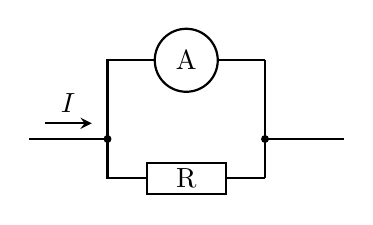
\begin{tikzpicture}[>=stealth, thick]
    % Asosiy kirish simi va tok yo'nalishi
    \draw (0,0) -- (1,0);
    \draw[->] (0.2,0.2) -- (0.8,0.2) node[midway, above] {$I$};

    % Tarmoqlanish nuqtasi (chapda)
    \draw (1,0) -- (1,1) -- (1.5,1); % Yuqoriga - ampermetrga
    \draw (1,0) -- (1,-0.5) -- (1.5,-0.5); % Pastga - shuntga

    % Ampermetr (yuqori tarmoq)
    \draw (2,1) circle (0.4) node {A};
    \draw (1.5,1) -- (1.6,1);
    \draw (2.4,1) -- (3,1);

    % Shunt qarshiligi (pastki tarmoq)
    \draw (1.5,-0.7) rectangle (2.5,-0.3) node[midway] {R};
    \draw (2.5,-0.5) -- (3,-0.5);

    % Birlashish nuqtasi (o'ngda)
    \draw (3,1) -- (3,-0.5);
    \draw (3,0) -- (4,0);
    \filldraw (1,0) circle (1pt);
    \filldraw (3,0) circle (1pt);

\end{tikzpicture}

\begin{enumerate}[label=\Alph*)]
\item 500
\item 120
\item 300
\item 200

\end{enumerate}

\item Ichki qarshiligi $180~\Omega$ bo‘lgan ampermetrning o‘lchash chegarasini $9$ marta oshirish uchun unga ulanadigan shuntning qarshiligi qanday bo‘lishi kerak ($\Omega$)?
\begin{enumerate}[label=\Alph*)]
\item 16,1
\item 18
\item 14
\item 22,5
\end{enumerate}

\item Ampermetrning ichki qarshiligi $12~\Omega$ bo‘lib, u $2,5$ A gacha tokni o‘lchashga mo‘ljallangan. Shu ampermetr bilan $15$ A gacha tokni o‘lchash uchun unga necha $\Omega$ li shunt ulash kerak?
\begin{enumerate}[label=\Alph*)]
\item 3,1
\item 1,1
\item 2,4
\item 4,2

\end{enumerate}

\item Zanjirga ulangan ampermetrning ichki qarshiligi $11~\Omega$ va shuntning qarshiligi $2,2~\Omega$. Ampermetr $13$ A tokni ko‘rsatsa, zanjirdagi tok kuchi necha Amperga teng bo‘ladi?
\begin{enumerate}[label=\Alph*)]
\item 78
\item 66
\item 20
\item 82
\end{enumerate}

\item Ikkita bir xil shuntlardan iborat ampermetrga ulansa, uning bo‘lim qiymati $3$ marta ortadi. Agar ikkala shunt ampermetrga parallel ulansa, uning o‘lchash chegarasi necha marta ortadi?
\begin{enumerate}[label=\Alph*)]
\item 3
\item 4
\item 5
\item 2,5
\end{enumerate}

\item Ikkita bir xil shunt o‘zaro ketma-ket ulanib, so‘ngra ampermetrga ulansa, uning o‘lchash chegarasi $4,5$ marta ortadi. Ikkala shunt ampermetrga parallel ulanganida ampermetrning o‘lchash chegarasi necha marta ortadi?
\begin{enumerate}[label=\Alph*)]
\item 6,5
\item 9
\item 15
\item 18
\end{enumerate}

\item Qarshiligi $0,04~\Omega$ bo‘lgan ampermetrga uzunligi $15$ cm va ko‘ndalang kesim yuzi $3$ mm$^2$ bo‘lgan mis sim parallel ulangan. Ampermetr $0,17$ A tokni ko‘rsatadi. Simdagi tok kuchini toping (A). Misning solishtirma qarshiligi $1,7\cdot10^{-8}~\Omega\cdot$m.
\begin{enumerate}[label=\Alph*)]
\item 2,8
\item 4
\item 5
\item 8
\end{enumerate}

\item Voltmetrning ichki qarshiligi $300~\Omega$. Unga $1200~\Omega$ qo‘shimcha qarshilik ulansa, shkala bo‘lim qiymati necha marta o‘zgaradi?
\begin{enumerate}[label=\Alph*)]
\item 3
\item 4
\item 5
\item 6
\end{enumerate}

\item Voltmetrning ichki qarshiligi $2$ k$\Omega$ bo‘lib, u $8$ V ni o‘lchashga mo‘ljallangan. Shu voltmetrga qanday qo‘shimcha qarshilik (k$\Omega$) ulanganda, u bilan $40$ V kuchlanishni o‘lchash mumkin bo‘ladi?
\begin{enumerate}[label=\Alph*)]
\item 5
\item 12
\item 18
\item 8
\end{enumerate}

\item Qarshiligi $1600~\Omega$ bo‘lgan voltmetr $15$ V gacha kuchlanishni o‘lchashga mo‘ljallangan. Shu voltmetr bilan $210$ V gacha kuchlanishni o‘lchash uchun unga qanday qo‘shimcha qarshilik ulash kerak ($\Omega$)?
\begin{enumerate}[label=\Alph*)]
\item 150
\item 20,8
\item 30
\item 27
\end{enumerate}

\item $15$ V kuchlanishni o‘lchashga mo‘ljallangan voltmetr bilan $270$ V kuchlanishni o‘lchash uchun unga qanday qarshilik ulash kerak ($\Omega$)? Voltmetrning qarshiligi $300~\Omega$ ga teng.
\begin{enumerate}[label=\Alph*)]
\item 5400
\item 5500
\item 5600
\item 5100
\end{enumerate}

\item $20$ V kuchlanishni o‘lchashga mo‘ljallangan voltmetr bilan $150$ V kuchlanishni o‘lchash uchun unga qanday qo‘shimcha qarshilik ($\Omega$) ulash kerak? $R_v=200~\Omega$.
\begin{enumerate}[label=\Alph*)]
\item 1300
\item 1500
\item 1400
\item 1600
\end{enumerate}

\item Ichki qarshiligi $2800~\Omega$ bo‘lgan voltmetr elektr tarmog‘iga ulanganda, $120$ V kuchlanishni ko‘rsatdi. Voltmetrga necha $\Omega$ qarshilik ketma-ket ulansa, u $80$ V ni ko‘rsatadi?
\begin{enumerate}[label=\Alph*)]
\item 2700
\item 1700
\item 2100
\item 1400
\end{enumerate}

\item Sxemada $R_1=800~\Omega$, $R_2=1000~\Omega$ va shu zanjirning umumiy qarshiligi $480~\Omega$ bo‘lsa, voltmetrning o‘lchash chegarasi necha marta oshirilgan?

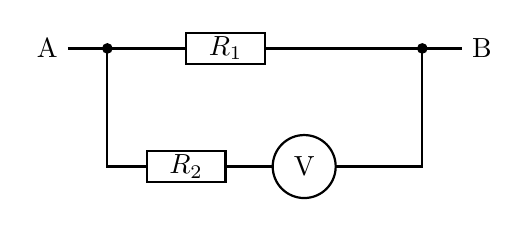
\begin{tikzpicture}[>=stealth, thick]
    % Asosiy tarmoq va A, B nuqtalari
    \draw (0,0) node[left] {A} -- (0.5,0);
    \draw (4.5,0) -- (5,0) node[right] {B};

    % Yuqori tarmoq (R1 qarshilik bilan)
    \draw (0.5,0) -- (1.5,0);
    \draw (1.5,-0.2) rectangle (2.5,0.2) node[midway] {$R_1$};
    \draw (2.5,0) -- (4.5,0);

    % Pastki tarmoq (R2 qarshilik va V voltmetr bilan)
    \draw (0.5,0) -- (0.5,-1.5) -- (1,-1.5);
    \draw (1,-1.7) rectangle (2,-1.3) node[midway] {$R_2$};
    \draw (2,-1.5) -- (2.6,-1.5);
    \draw (3,-1.5) circle (0.4) node {V};
    \draw (3.4,-1.5) -- (4.5,-1.5) -- (4.5,0);

    % Tugun nuqtalarini belgilash
    \filldraw (0.5,0) circle (1.5pt);
    \filldraw (4.5,0) circle (1.5pt);

\end{tikzpicture}

\begin{enumerate}[label=\Alph*)]
\item 3
\item 4
\item 5
\item 6
\end{enumerate}

\end{enumerate}

\begin{table}[!ht]
\centering
\begin{tabular}{|c|c|c|c|c|c|c|c|c|c|}
\hline
1d & 2c & 3b & 4d & 5c & 6a & 7c & 8c & 9d & 10c \\ \hline
11d & 12b & 13d & 14a & 15d & 16d &  &  &  &  \\ \hline
\end{tabular}
\end{table}

\section{Tok manbalarini ketma-ket va parallel ulash}



\begin{enumerate}

\item Har birining EYKi $6$ V va ichki qarshiligi $0,6~\Omega$ bo‘lgan ikkita akkumulyator ketma-ket ulanganda, $2$ A tok bo‘lishi uchun tashqi zanjirdagi qarshilik qanday bo‘lishi kerak ($\Omega$)?
\begin{enumerate}[label=\Alph*)]
\item 48
\item 18
\item 4,8
\item 2
\end{enumerate}

\item Tashqi zanjirdagi kuchlanish $100$ V va tok kuchi $5$ A bo‘lishi uchun EYKi $2,5$ V dan va ichki qarshiligi $0,1~\Omega$ dan bo‘lgan manbalardan nechtasini ketma-ket ulab, batareya tuzish kerak bo‘ladi?
\begin{enumerate}[label=\Alph*)]
\item 25
\item 36
\item 40
\item 50
\end{enumerate}

\item Rasmda ko‘rsatilgan elektr zanjirda $\varepsilon_1=6$ V, $\varepsilon_2=18$ V, $R=3~\Omega$. Manbalar ichki qarshilikka ega emas. Zanjirdagi tok kuchi necha Amper?

\begin{circuitikz}[european]
\draw
  % Chap tomondagi vertikal rezistor R
  (0,0) to[R=R] (0,3)
  
  % Yuqori tomondagi tok manbai epsilon_1
  % Musbat qutbi o'ng tomonda
  (0,3) to[battery1, l=$\varepsilon_1$] (4,3)
  
  % O'ng tomondagi vertikal rezistor R
  (4,3) to[R=R] (4,0)
  
  % Pastki tomondagi tok manbai epsilon_2
  % Musbat qutbi chap tomonda
  (4,0) to[battery1, l=$\varepsilon_2$] (0,0);
\end{circuitikz}

\begin{enumerate}[label=\Alph*)]
\item 8
\item 6
\item 4
\item 3
\end{enumerate}

\item $\varepsilon_1=5$ V, $\varepsilon_2=3$ V, $\varepsilon_3=4$ V, $r=1~\Omega$ va $R=7~\Omega$ bo‘lsa, $R$ qarshilikdagi kuchlanishning tushishi necha Volt bo‘ladi (rasmga q.)?

\begin{circuitikz}[european]
\draw
  % Pastki tarmoq: Tashqi rezistor R
  (0,0) to[R=R] (4,0)
  
  % O'ng tarmoq: Tok manbai epsilon_3 va ichki qarshilik r
  % Qutblari: yuqorida +, pastda -
  (4,0) to[battery1, l_=$\varepsilon_3$, i^=$r$] (4,3)
  
  % Yuqori tarmoq: Tok manbai epsilon_2 va ichki qarshilik r
  % Qutblari: chapda +, o'ngda -
  (4,3) to[battery1, l=$\varepsilon_2$, i=$r$] (0,3)
  
  % Chap tarmoq: Tok manbai epsilon_1 va ichki qarshilik r
  % Qutblari: yuqorida +, pastda -
  (0,0) to[battery1, l=$\varepsilon_1$, i=$r$] (0,3);
\end{circuitikz}

\begin{enumerate}[label=\Alph*)]
\item 14
\item 1,4
\item 7
\item 0,7
\end{enumerate}

\item Rasmda ko‘rsatilgan elektr zanjirda $\varepsilon_1=6$ V, $\varepsilon_2=12$ V va $R=6~\Omega$. Manbalarning ichki qarshiligi bo‘lmasa, zanjirdagi tok kuchi necha Amper bo‘ladi?

\begin{circuitikz}[european]
\draw
  % Chap vertical tarmoq: epsilon_1 manbasi
  % Musbat qutbi (+) pastda joylashgan
  (0,0) to[battery1, l=$\varepsilon_1$] (0,3)
  
  % Yuqori horizontal tarmoq: R rezistor
  (0,3) -- (1.5,3) to[R=R] (2.5,3) -- (4,3)
  
  % O'ng vertical tarmoq: epsilon_2 manbasi
  % Musbat qutbi (+) pastda joylashgan
  (4,3) to[battery1, l_=$\varepsilon_2$] (4,0)
  
  % Pastki horizontal tutashtiruvchi sim
  (4,0) -- (0,0);
\end{circuitikz}

\begin{enumerate}[label=\Alph*)]
\item 1
\item 2
\item 3
\item 4
\end{enumerate}

\item Rasmda ko‘rsatilgan zanjirdagi tok kuchi necha Amperga teng? $\varepsilon_1=\varepsilon_2=\varepsilon_3=6$ V, $r_1=r_2=r_3=0,5~\Omega, R=1,5~\Omega$.

\begin{circuitikz}[european]
\draw
  % Yuqori tarmoq: epsilon_1 va epsilon_2 manbalari
  % epsilon_1 musbat qutbi o'ngda, epsilon_2 musbat qutbi chapda
  (0,3) to[battery1, l=$\varepsilon_1$] (2,3)
        to[battery1, l=$\varepsilon_2$, invert] (4,3)
  
  % O'ng tarmoq: R rezistor
  (4,3) to[R=R] (4,0)
  
  % Pastki tarmoq: epsilon_3 manbasi
  % Musbat qutbi chapda joylashgan
  (4,0) to[battery1, l_=$\varepsilon_3$] (0,0)
  
  % Chap tarmoq: tutashtiruvchi sim
  (0,0) -- (0,3);
\end{circuitikz}

\begin{enumerate}[label=\Alph*)]
\item 1,5
\item 2
\item 3
\item 6
\end{enumerate}

\item Uchta tok manbai va bitta qarshilikdan rasmda ko‘rsatilgandek zanjir tuzilgan. Agar $\varepsilon_1=3,5$ V, $\varepsilon_2=1,5$ V, $\varepsilon_3=2$ V, $r_1=r_2=r_3=0,2~\Omega$, va $R=4,4~\Omega$ bo‘lsa, $R$ qarshilikdan o‘tayotgan tok kuchi necha Amper?

\begin{circuitikz}[european]
\draw
  % Yuqori tarmoq: epsilon_1 va epsilon_2 manbalari
  % epsilon_1 (+) o'ngda, epsilon_2 (+) chapda (manbadagi rasmga ko'ra)
  (0,3) to[battery1, l=$\varepsilon_1$] (2,3)
        to[battery1, l=$\varepsilon_2$, invert] (4,3)
  
  % O'ng vertical tarmoq: Tashqi rezistor R
  (4,3) to[R=R] (4,0)
  
  % Pastki tarmoq: epsilon_3 manbasi
  % (+) chapda joylashgan (4,0 dan 0,0 ga qarab)
  (4,0) to[battery1, l_=$\varepsilon_3$] (0,0)
  
  % Chap vertical tarmoq: tutashtiruvchi sim
  (0,0) -- (0,3);
\end{circuitikz}

\begin{enumerate}[label=\Alph*)]
\item 0,6
\item 0,9
\item 1,6
\item 0,8
\end{enumerate}

\item Sxemada $\varepsilon_1=2$ V, $\varepsilon_2=1$ V, $r_1=r_2=1~\Omega, R=2~\Omega$. Tashqi qarshilikdagi kuchlanishning tushishini toping (V).

\begin{circuitikz}[european]
\draw
  % Yuqori horizontal tarmoq: Ikkita tok manbai ketma-ket
  % Har ikkala manbaning musbat qutbi (+) o'ng tomonga yo'nalgan
  (0,3) to[battery1, l=$\varepsilon_1$, annotation=$r_1$] (2,3)
        to[battery1, l=$\varepsilon_2$, annotation=$r_2$] (4,3)
  
  % O'ng vertical tutashtiruvchi sim
  (4,3) -- (4,0)
  
  % Pastki horizontal tarmoq: Tashqi rezistor R
  (4,0) to[R=R] (0,0)
  
  % Chap vertical tutashtiruvchi sim
  (0,0) -- (0,3);
\end{circuitikz}

\begin{enumerate}[label=\Alph*)]
\item 0,5
\item 1
\item 1,5
\item 2
\end{enumerate}

\item Kondensatorlardagi kuchlanishlar qanday (V)? $\varepsilon_1=12$ V; $\varepsilon_2=13$ V; $C_1=3~\mu$F; $C_2=7~\mu$F. 

\begin{circuitikz}[european]
\draw
  % Yuqori horizontal tarmoq: epsilon_1 manbasi
  % Musbat qutbi o'ng tomonda
  (0,3) to[battery1, l=$\varepsilon_1$] (4,3)
  
  % O'ng vertical tarmoq: Kondensator C2
  (4,3) to[C, l=$C_2$] (4,0)
  
  % Pastki horizontal tarmoq: epsilon_2 manbasi
  % Musbat qutbi chap tomonda
  (4,0) to[battery1, l_=$\varepsilon_2$] (0,0)
  
  % Chap vertical tarmoq: Kondensator C1
  (0,0) to[C, l=$C_1$] (0,3);
\end{circuitikz}

\begin{enumerate}[label=\Alph*)]
\item 6,5; 18,5
\item 7; 18
\item 18; 7
\item 17,5; 7,5
\end{enumerate}

\item Sxemada EYK lar $\varepsilon_1=3$ V va $\varepsilon_2=2$ V, ichki qarshiliklar $r=0,5~\Omega$ bo‘lsa, voltmetr necha Voltni ko‘rsatadi? $R_V = \infty$.

\begin{circuitikz}[european]
\draw
  % Yuqori tarmoq: epsilon_1 va r
  % Musbat qutb o'ng tomonda
  (0,2) to[battery1, l=$\varepsilon_1$] (1.5,2) to[R=r] (3,2)
  
  % O'rta tarmoq: epsilon_2 va r
  % Musbat qutb o'ng tomonda
  (0,1) to[battery1, l=$\varepsilon_2$] (1.5,1) to[R=r] (3,1)
  
  % Chap va o'ng vertikal tutashtiruvchi simlar
  (0,2) -- (0,1) -- (0,0)
  (3,2) -- (3,1) -- (3,0)
  
  % Pastki qism: Voltmetr (V)
  (0,0) to[voltmeter, l=V] (3,0);
\end{circuitikz}

\begin{enumerate}[label=\Alph*)]
\item 1
\item 2,5
\item 2
\item 3
\end{enumerate}

\item Sxemada EYK lar $\varepsilon_1=3$ V va $\varepsilon_2=2$ V, ichki qarshiliklar $r=0,5~\Omega$ bo‘lsa, voltmetr necha Voltni ko‘rsatadi? $R_V = \infty$. 

\begin{circuitikz}[european]
\draw
  % Yuqori tarmoq: epsilon_1 va r
  % Musbat qutb o'ng tomonda
  (0,2) to[battery1, l=$\varepsilon_1$] (1.5,2) to[R=r] (3,2)
  
  % O'rta tarmoq: epsilon_2 va r
  % Musbat qutb chap tomonda (invert orqali)
  (0,1) to[battery1, l=$\varepsilon_2$, invert] (1.5,1) to[R=r] (3,1)
  
  % Chap va o'ng vertikal tutashtiruvchi simlar
  (0,2) -- (0,1) -- (0,0)
  (3,2) -- (3,1) -- (3,0)
  
  % Pastki qism: Voltmetr (V)
  (0,0) to[voltmeter, l=V] (3,0);
\end{circuitikz}

\begin{enumerate}[label=\Alph*)]
\item 0,5
\item 1
\item 2
\item 3
\end{enumerate}

\item Elektr yurituvchi kuchlari teng, ichki qarshiliklari $2$ marta farq qiladigan tok manbalari rasmdagidek ulangan. Voltmetrning ko‘rsatishini toping. $R_V = \infty$.

\begin{circuitikz}[european]
\draw
  % Chap tarmoq: epsilon va r
  (0,0) to[battery1, l=$\varepsilon$] (0,1.5)
        to[R=r] (0,3)
  
  % O'rta tarmoq: Voltmetr (V)
  (2,0) to[voltmeter, l=V, *-*] (2,3)
  
  % O'ng tarmoq: epsilon va 2r
  (4,0) to[battery1, l_=$\varepsilon$] (4,1.5)
        to[R=2r] (4,3)
  
  % Yuqori va pastki horizontal tutashtiruvchi simlar
  (0,3) -- (4,3)
  (0,0) -- (4,0);
\end{circuitikz}

\begin{enumerate}[label=\Alph*)]
\item 0
\item $\varepsilon/2$
\item $\varepsilon$
\item $\varepsilon/3$
\end{enumerate}

\item EYUK $1,5$ V va $2$ V bo‘lgan elementlar bir xil ishorali qutblari bilan ulangan. Batareya klemmalariga ulangan voltmetr $1,7$ V kuchlanishni ko‘rsatdi. Elementlar ichki qarshiliklari nisbatini toping.
\begin{enumerate}[label=\Alph*)]
\item 1
\item 2/3
\item 2
\item 1/3
\end{enumerate}

\item EYK lari $\varepsilon_1$ va $\varepsilon_2$ bo‘lgan manbalar bir xil qutblari bilan o‘zaro parallel ulangan. Agar manbalarning ichki qarshiliklari teng bo‘lsa, manba qutblaridagi potensiallar farqi qanday?
\begin{enumerate}[label=\Alph*)]
\item $\varepsilon_1 + \varepsilon_2$
\item $(\varepsilon_1 - \varepsilon_2)/2$
\item 0
\item $(\varepsilon_1 + \varepsilon_2)/2$
\end{enumerate}

\end{enumerate}



\begin{table}[!ht]
\centering
\begin{tabular}{|c|c|c|c|c|c|c|c|c|c|}
\hline
1d & 2d & 3d & 4b & 5c & 6d & 7c & 8b & 9c & 10a \\ \hline
11b & 12d & 13c & 14d &  &  &  &  &  &  \\ \hline
\end{tabular}
\end{table}



\section{O`zgarmas tokning ishi va quvvati. Joul-Lens qonuni}


\begin{enumerate}

\item Berilgan formulalardan qaysi biri Joul–Lens qonunini ifodalaydi? 
\begin{enumerate}[label=\Alph*)]
\item $Q = I^2Rt$
\item $Q = \lambda m$
\item $Q = cm(t_2 - t_1)$
\item $Q = A + \Delta U$
\end{enumerate}

\item Qarshiligi $2~\Omega$ bo‘lgan simdan $15$ A tok o‘tadi. $2$ minut ichida unda qancha energiya ajraladi (kJ)? 
\begin{enumerate}[label=\Alph*)]
\item 27
\item 54
\item 450
\item 900
\end{enumerate}

\item $50~\Omega$ qarshilikli o‘tkazgich orqali $10$ minut davomida qanday tok o‘tkazilganda, $120$ kJ issiqlik ajralib chiqadi (A)?
\begin{enumerate}[label=\Alph*)]
\item 2
\item 3
\item 4
\item 5
\end{enumerate}

\item Qarshiligi $12~\Omega$ bo‘lgan o‘tkazgich $120$ V kuchlanishli tarmoqqa ulandi. O‘tkazgichda $10$ min ichida qancha issiqlik ajraladi?
\begin{enumerate}[label=\Alph*)]
\item 72 kJ
\item 0,72 kJ
\item 720 kJ
\item 7,2 MJ
\end{enumerate}

\item Agar $R_1 = R_2 = R_3$ bo‘lsa, rasmda ko‘rsatilgan rezistorlardan bir xil vaqt davomida ajralib chiqayotgan issiqlik miqdorlarining nisbati $Q_1 : Q_2 : Q_3$ ni aniqlang.

\begin{circuitikz}[european]
\draw
  % Kirish simi va R1 rezistori (ketma-ket qism)
  (0,0) to[R=$R_1$, *-] (2,0)
  
  % Parallel tarmoqlanish boshlanishi
  (2,0) -- (2,0.7) to[R=$R_2$] (4,0.7) -- (4,0)
  (2,0) -- (2,-0.7) to[R=$R_3$] (4,-0.7) -- (4,0)
  
  % Chiqish simi va tok kuchi I
  (4,0) -- (5.5,0)
  (4.5,0) node[currarrow, label=above:$I$] {};
\end{circuitikz}

\begin{enumerate}[label=\Alph*)]
\item 4:1:1
\item 1:1:1
\item 4:4:1
\item 1:4:4
\end{enumerate}

\item $R$ va $2R$ qarshiliklar o‘zgarmas kuchlanish manbaiga parallel ulangan. $R$ qarshilikda $100$ J issiqlik miqdori ajralganda, $2R$ qarshilikda qancha issiqlik miqdori ajraladi (J)?
\begin{enumerate}[label=\Alph*)]
\item 400
\item 200
\item 100
\item 50
\end{enumerate}


\item Elektr choynakning ikki chulg‘ami bor. Ulardan biri manbaga ulanganda choynakdagi suv $30$ minutda, ikkinchisi ulanganda esa $20$ minutda qaynaydi. Agar ikkala chulg‘am manbaga ketma-ket ulansa, choynakdagi suv necha minutda qaynaydi?
\begin{enumerate}[label=\Alph*)]
\item 25
\item 30
\item 40
\item 50
\end{enumerate}

\item Elektr isitkich bir xil $R$ qarshilikli uchta spiralga ega. Agar uchala spiral parallel ulansa, unga qo‘yilgan idishdagi suv $6$ minutda qaynaydi. Spirallar rasmda ko‘rsatilgandek ulansa (ikki spiral parallel va biri ularga ketma-ket), shu suv necha minutda qaynaydi?
\begin{enumerate}[label=\Alph*)]
\item 24
\item 4
\item 12
\item 16
\end{enumerate}


\item Chulg‘amning qarshiligi $50~\Omega$ bo‘lgan elektr choynakda temperaturasi $0^\circ$C bo‘lgan $600$~cm$^3$ suv bor. Agar tarmoqning kuchlanishi $200$~V, choynakning FIK $60\%$ bo‘lsa, undagi hamma suvni qaynatib, bug‘ga aylantirish uchun necha minut vaqt kerak bo‘ladi? Suv uchun $c=4,2$~kJ/(kg$\cdot$K), $r=2,3$~MJ/kg.
\begin{enumerate}[label=\Alph*)]
\item 57
\item 28
\item 32
\item 41
\end{enumerate}

\item Qaysi qarshilikda eng ko‘p issiqlik ajraladi? $R_1=1~\Omega, R_2=R_3=2~\Omega, R_4=4~\Omega$. (Rasmga qarang)

\begin{circuitikz}[european]
\draw
  % Kirish simi va tugun nuqtasi
  (0,0) -- (1,0) to[short, *-] (1,0)
  
  % Yuqori tarmoq: R1 va R2 ketma-ket
  (1,0) -- (1,1) to[R=$R_1$] (3,1) to[R=$R_2$] (5,1) -- (5,0)
  
  % Pastki tarmoq: R3 va R4 ketma-ket
  (1,0) -- (1,-1) to[R=$R_3$] (3,-1) to[R=$R_4$] (5,-1) -- (5,0)
  
  % Chiqish simi va tugun nuqtasi
  (5,0) to[short, -*] (6,0);
\end{circuitikz}


\begin{enumerate}[label=\Alph*)]
\item $R_1$ da
\item $R_2$ da
\item $R_3$ da
\item $R_4$ da
\end{enumerate}

\item Qarshiligi $R_1$ bo‘lgan qaynatgich biror miqdor suvni $t_1$ vaqtda qaynatadi. Qarshiligi $R_2$ bo‘lgan qaynatgich esa shu sharoitda o‘sha suvni $t_2$ vaqtda qaynatadi. Ikkala qaynatgich parallel ulansa o‘sha suv qanday vaqtda qaynaydi?
\begin{enumerate}[label=\Alph*)]
\item $t_1+t_2$
\item $\frac{t_1 t_2}{t_1+t_2}$
\item $\sqrt{t_1 t_2}$
\item $\frac{t_1+t_2}{2}$
\end{enumerate}

\item Elektr choynakda ikkita chulg‘am bor. Birinchi chulg‘am ulanganda, suv $t_1$ vaqtda, ikkinchisi ulanganda, $t_2$ vaqtda qaynaydi. Ikkala chulg‘am ketma-ket ulanganda qaynash vaqti, ular parallel ulangandagi qaynash vaqtidan necha marta katta bo‘ladi?
\begin{enumerate}[label=\Alph*)]
\item $\frac{2t_1 t_2}{t_1+t_2}$
\item $\frac{t_1+t_2}{t_1 t_2}$
\item $\frac{(t_1+t_2)^2}{t_1 t_2}$
\item $\frac{t_1-t_2}{t_1+t_2}$
\end{enumerate}

\item Ikkita bir xil elektr plita parallel ulansa, suv $t$ vaqtda qaynaydi. Shu plitalar ketma-ket ulansa, shu suv qancha vaqtda qaynaydi?
\begin{enumerate}[label=\Alph*)]
\item $2t$
\item $t/2$
\item $t/3$
\item $4t$
\end{enumerate}


\item Elektr choynakning ikkita chulg‘ami bor. Ulardan biri manbaga ulanganda choynakdagi suv $30$ minutda, ikkinchisi ulanganda esa $20$ minutda qaynaydi. Agar ikkala chulg‘am manbaga ketma-ket ulansa, choynakdagi suv necha minutda qaynaydi?
\begin{enumerate}[label=\Alph*)]
\item 25
\item 30
\item 40
\item 50
\end{enumerate}

\item Elektr isitkich bir xil $R$ qarshilikli uchta tarmoqqa ega. Agar har uchala tarmoq o‘zaro parallel ulansa, unga qo‘yilgan idishdagi suv $6$ min da qaynaydi. Tarmoqlar o‘zaro ketma-ket ulanganida shu suv necha minutda qaynar edi?
\begin{enumerate}[label=\Alph*)]
\item 60
\item 54
\item 44
\item 38
\end{enumerate}

\item Elektr isitkich bir xil $R$ qarshilikli uchta spiralga ega. Agar uchala spiral parallel ulansa, unga qo‘yilgan idishdagi suv $6$ minutda qaynaydi. Spirallar rasmda ko‘rsatilgandek ulansa, shu suv necha minutda qaynaydi?

\begin{circuitikz}[european]
\draw
  % Kirish tugun nuqtasi
  (0,0) to[short, *-] (0.5,0)
  
  % Yuqori tarmoq: ikkita R rezistor ketma-ket
  (0.5,0) -- (0.5,0.8) to[R=R] (2.5,0.8) to[R=R] (4.5,0.8) -- (4.5,0)
  
  % Pastki tarmoq: bitta R rezistor
  (0.5,0) -- (0.5,-0.8) to[R=R] (4.5,-0.8) -- (4.5,0)
  
  % Chiqish tugun nuqtasi
  (4.5,0) to[short, -*] (5,0);
\end{circuitikz}

\begin{enumerate}[label=\Alph*)]
\item 24
\item 4
\item 12
\item 16
\end{enumerate}

\item Elektr plita suvni $10$ minutda qaynatadi. Spiralning bir qismi uzilgandan so‘ng, shu suvni $12$ min da qaynatdi. Spiral dastlabki uzunligining qanday qismiga kaltalashgan? Tok kuchini o‘zgarmas deb hisoblang.
\begin{enumerate}[label=\Alph*)]
\item $1/3$
\item $1/8$
\item $1/12$
\item $1/6$
\end{enumerate}

\item Suv ikkita bir xil spiral bilan isitiladi. Spirallar dastlab o‘zgarmas kuchlanish manbayiga $t$ vaqt davomida parallel, keyin xuddi shuncha vaqt ketma-ket ulandi. Agar dastlabki $t$ vaqtda suvning temperaturasi $10^\circ$C ga ortgan bo‘lsa, $2t$ umumiy vaqtda qanchaga ($^\circ$C) ortgan?
\begin{enumerate}[label=\Alph*)]
\item 20
\item 15
\item 17,5
\item 12,5
\end{enumerate}




\end{enumerate}



\begin{table}[!ht]
\centering
\begin{tabular}{|c|c|c|c|c|c|c|c|c|c|}
\hline
1a & 2d & 3b & 4a & 5d & 6c & 7d & 8c & 9a & 10a \\ \hline
11a & 12d & 13b & 14a & 15b & 16b & 17c & 18d & & \\ \hline
\end{tabular}
\end{table}



\section{Turli muhitlarda elektr toki}

\subsection*{Metallarda elektr toki}



\begin{enumerate}

\item Metallarda elektr tokini qanday zarralar oqimi hosil qiladi?
\begin{enumerate}[label=\Alph*)]
\item elektronlar.
\item ionlar.
\item kovaklar.
\item molekulalar.
\end{enumerate}

\item Metallarda elektr toki qanday elektr zaryadlarning tartibli harakati tufayli hosil bo‘ladi?
\begin{enumerate}[label=\Alph*)]
\item musbat va manfiy ionlar, elektronlar.
\item musbat va manfiy ionlar.
\item faqat elektronlar.
\item elektron va musbat ionlar.
\end{enumerate}

\item Metallardan elektr toki o‘tganda tokning qanday ta’sirlari jarayon bo‘ladi?
\begin{enumerate}[label=\Alph*)]
\item faqat issiqlik va magnit ta’sirlari.
\item faqat issiqlik va kimyoviy ta’sirlari.
\item faqat kimyoviy va magnit ta’sirlari.
\item issiqlik, magnit va kimyoviy ta’sirlari.
\end{enumerate}

\item Mandelshtam–Papaleksi, Styuart–Tolmen tajribalari tasdiqlashicha, metallarda elektr o‘tkazuvchanlik ...
\begin{enumerate}[label=\Alph*)]
\item elektronli.
\item ionli.
\item elektron-ionli.
\item elektron-kovakli.
\end{enumerate}

\item Metallar o‘tkazuvchanligining klassik elektron nazariyasiga ko‘ra $j/en$ ifoda qaysi kattalikni beradi? ($j$ – tok zichligi, $e$ – elektron zaryadi, $n$ – elektronlarning konsentratsiyasi).
\begin{enumerate}[label=\Alph*)]
\item solishtirma qarshilik.
\item tok kuchi.
\item solishtirma o‘tkazuvchanlik.
\item elektronlar tartibli harakatining o‘rtacha tezligi.
\end{enumerate}

\item Metallarning harorati ortishi bilan elektr qarshiligi qanday o‘zgaradi?
\begin{enumerate}[label=\Alph*)]
\item chiziqli oshadi.
\item o‘zgarmaydi.
\item chiziqli kamayadi.
\item keskin oshadi.
\end{enumerate}

\item O‘tkazgich temperaturasini o‘zgarmas qoldirib, undan o‘tayotgan tok kuchini oshirsak, uning qarshiligi ...
\begin{enumerate}[label=\Alph*)]
\item oshishi ham, kamayishi ham mumkin.
\item oshadi.
\item kamayadi.
\item o‘zgarmaydi.
\end{enumerate}


\item G‘altakning mis simi 25$^\circ$C da 11 $\Omega$ qarshilikka ega. 100$^\circ$C gacha isitilganda uning qarshiligi necha $\Omega$ bo‘lishini baholang. Mis qarshiligining temperaturaviy koeffitsienti $4 \cdot 10^{-3}$ K$^{-1}$.
\begin{enumerate}[label=\Alph*)]
\item 15.
\item 14.
\item 13.
\item 12.
\end{enumerate}

\item Mis simning 50$^\circ$C dagi qarshiligi 2 $\Omega$ bo‘lsa, uning 100$^\circ$C dagi qarshiligi necha $\Omega$ bo‘ladi? Mis uchun qarshilikning temperaturaviy koeffitsienti 0,004 K$^{-1}$.
\begin{enumerate}[label=\Alph*)]
\item 0,5.
\item 4,66.
\item 1,16.
\item 2,33.
\end{enumerate}

\item 0$^\circ$C temperaturada platinali termometrning qarshiligi 6 $\Omega$, 100$^\circ$C da esa 8,4 $\Omega$ ga teng. Qanday temperaturada ($^\circ$C) uning qarshiligi 14,4 $\Omega$ ga teng bo‘ladi?
\begin{enumerate}[label=\Alph*)]
\item 300.
\item 250.
\item 200.
\item 350.
\end{enumerate}

\item Lampa tolasining 0$^\circ$C haroratdagi qarshiligi 2000$^\circ$C haroratdagi qarshiligidan 15 marta kichik. Tola qarshiligining temperaturaviy koeffitsienti qanday ($10^{-3}$ K$^{-1}$)?
\begin{enumerate}[label=\Alph*)]
\item 3,5.
\item 7.
\item 14.
\item 21.
\end{enumerate}

\item 0$^\circ$C da qarshiligi 80 $\Omega$ bo‘lgan o‘tkazgichdan tok o‘tishi natijasida uning qarshiligi 4 $\Omega$ ga o‘zgardi. Agar qarshilikning termik koeffitsienti 0,004 1/K ga teng bo‘lsa, uning temperaturasi qanchaga ($^\circ$C) o‘zgargan?
\begin{enumerate}[label=\Alph*)]
\item 12,5.
\item 50.
\item 20.
\item 25.
\end{enumerate}

\item O‘ta o‘tkazuvchanlik hodisasini kim kashf etgan?
\begin{enumerate}[label=\Alph*)]
\item X.K. Onnes.
\item N.N. Bogolyubov.
\item L.N. Kuper.
\item J. Bardin.
\end{enumerate}

\item O‘ta o‘tkazuvchanlik birinchi marta qaysi moddada kashf etilgan?
\begin{enumerate}[label=\Alph*)]
\item mis.
\item alyuminiy.
\item temir.
\item simob.
\end{enumerate}



\end{enumerate}


\begin{table}[!ht]
\centering
\begin{tabular}{|c|c|c|c|c|c|c|}
\hline
1a & 2c & 3a & 4a & 5d & 6a & 7d \\ \hline
8b & 9d & 10d & 11b & 12a & 13a & 14d \\ \hline
\end{tabular}
\end{table}


\subsection*{Yarim o`tkazgichlarda elektr toki}


\begin{enumerate}

\item Temperatura ortishi bilan yarimo‘tkazgichning qarshiligi ...
\begin{enumerate}[label=\Alph*)]
\item kamayadi.
\item o‘zgarmaydi.
\item ortadi.
\item avval ortadi, so‘ngra kamayadi.
\end{enumerate}

\item Yarimo‘tkazgichlarda elektr tokini qanday zarralar oqimi hosil qiladi? Eng to‘la javobni ko‘rsating.
\begin{enumerate}[label=\Alph*)]
\item elektronlar va kovaklar.
\item elektronlar va ionlar.
\item ionlar va kovaklar.
\item atomlar va elektronlar.
\end{enumerate}

\item Aralashmasiz yarimo‘tkazgichlar qanday turdagi o‘tkazuvchanlikka ega?
\begin{enumerate}[label=\Alph*)]
\item elektr tokini o‘tkazmaydilar.
\item teng miqdorda elektron va teshikli o‘tkazuvchanlikka.
\item asosan teshikli o‘tkazuvchanlikka.
\item asosan elektron o‘tkazuvchanlikka.
\end{enumerate}

\item Yarimo‘tkazgichda teshik va elektron uchrashganda nima hosil bo‘ladi?
\begin{enumerate}[label=\Alph*)]
\item musbat ion.
\item manfiy ion.
\item neytral atom.
\item musbat va manfiy ionlar.
\end{enumerate}

\item Yarimo‘tkazgichda elektron va teshik uchrashganda qanday hodisa yuz beradi?
\begin{enumerate}[label=\Alph*)]
\item energiya yutiladi.
\item musbat ion hosil bo‘ladi.
\item energiya ajraladi.
\item manfiy ion hosil bo‘ladi.
\end{enumerate}

\item Toza yarimo‘tkazgichdan elektronlarning tartibli harakati tufayli 1,7 mA tok o‘tmoqda. Yarimo‘tkazgichdan o‘tayotgan to‘la tok kuchi qanday (mA)?
\begin{enumerate}[label=\Alph*)]
\item 0.
\item 0,85.
\item 1,7.
\item 3,4.
\end{enumerate}

\item Yarimo‘tkazgichlarda donor aralashmasi bo‘lganda, ... ortadi. Mazkur jumladagi nuqtalar o‘rnini to‘ldiring.
\begin{enumerate}[label=\Alph*)]
\item kovaklar soni.
\item erkin pozitronlar soni.
\item erkin protonlar soni.
\item erkin elektronlar soni.
\end{enumerate}

\item Yarimo‘tkazgichlarda akseptor aralashmasi bo‘lganda, ... ortadi. Mazkur jumladagi nuqtalar o‘rnini to‘ldiring.
\begin{enumerate}[label=\Alph*)]
\item erkin protonlar soni.
\item erkin elektronlar soni.
\item kovaklar soni.
\item erkin pozitronlar soni.
\end{enumerate}

\item Yarimo‘tkazgich asosan teshikli o‘tkazuvchanlikka ega. Kristallda qanday aralashma bor?
\begin{enumerate}[label=\Alph*)]
\item asosan teshikli o‘tkazuvchanlikka ega yarimo‘tkazgich bo‘lmaydi.
\item akseptor aralashma.
\item aralashmalar yo‘q.
\item donor aralashma.
\end{enumerate}

\item Yarimo‘tkazgich asosan elektron o‘tkazuvchanlikka ega. Kristallda qanday aralashma bor?
\begin{enumerate}[label=\Alph*)]
\item donor aralashma.
\item akseptor aralashma.
\item aralashmalar yo‘q.
\item donor va akseptorlarning konsentratsiyalari teng.
\end{enumerate}

\item Donor aralashmali yarimo‘tkazgichlar qaysi turdagi o‘tkazuvchanlikka ega?
\begin{enumerate}[label=\Alph*)]
\item asosan elektronli.
\item asosan kovakli.
\item ham kovakli, ham elektronli (teng miqdorda).
\item ionli.
\end{enumerate}

\item Akseptor aralashmali yarimo‘tkazgichlar qanday tipdagi o‘tkazuvchanlikka ega?
\begin{enumerate}[label=\Alph*)]
\item asosan teshikli o‘tkazuvchanlikka.
\item asosan elektron o‘tkazuvchanlikka.
\item teng miqdorda elektron va teshikli o‘tkazuvchanlikka.
\item elektr tokini o‘tkazmaydi.
\end{enumerate}

\item Quyidagi lampalarning qaysi biri yonadi? (Rasmga qarang)

\begin{circuitikz}[european, scale=0.8]
% 1-chizma: O'zgarmas tok va kondensator
\draw (0,0) to[battery1] (0,2) to[lamp, l=1)] (2,2) to[C] (2,0) -- (0,0);

% 2-chizma: O'zgaruvchan tok va kondensator
\begin{scope}[xshift=4cm]
\draw (0,0) to[vsourcesin] (0,2) to[lamp, l=2)] (2,2) to[C] (2,0) -- (0,0);
\end{scope}

% 3-chizma: Diod (teskari ulanish)
\begin{scope}[yshift=-3.5cm]
\draw (0,0) to[battery1] (0,2) to[lamp, l=3)] (2,2) to[full diode, invert] (2,0) -- (0,0);
\end{scope}

% 4-chizma: Diod (to'g'ri ulanish)
\begin{scope}[xshift=4cm, yshift=-3.5cm]
\draw (0,0) to[battery1] (0,2) to[lamp, l=4)] (2,2) to[full diode] (2,0) -- (0,0);
\end{scope}
\end{circuitikz}

\begin{enumerate}[label=\Alph*)]
\item 2, 3.
\item 2, 4.
\item 2.
\item 3.
\end{enumerate}

\item Tranzistor qanday vazifani bajaradi?
\begin{enumerate}[label=\Alph*)]
\item o‘zgarmas tokni o‘zgaruvchan tokka aylantiradi.
\item o‘zgaruvchan tokni o‘zgarmas tokka aylantiradi.
\item elektr signallarini kuchaytiradi.
\item elektr zaryadlarini to‘playdi.
\end{enumerate}

\item Tranzistor nimalardan tashkil topgan?
\begin{enumerate}[label=\Alph*)]
\item emitter, baza va kollektordan.
\item emitter va kollektordan.
\item baza va emitterdan.
\item anod, katod va to‘rdan.
\end{enumerate}

\end{enumerate}


\begin{table}[!ht]
\centering
\begin{tabular}{|c|c|c|c|c|c|c|c|c|c|}
\hline
1a & 2a & 3b & 4c & 5c & 6d & 7d & 8c & 9b & 10a \\ \hline
11a & 12a & 13a & 14c & 15a & & & & & \\ \hline
\end{tabular}
\end{table}





\subsection*{Vakumda elektr toki}


\begin{enumerate}

\item Termoelektron emissiya nima?
\begin{enumerate}[label=\Alph*)]
\item qizdirilgan qattiq jism sirtidan musbat ionlarning nurlanishi.
\item atom yadrosining parchalanishi.
\item atomning elektron va ionga ajralishi.
\item qizdirilgan qattiq jism sirtidan elektronlarning nurlanishi.
\end{enumerate}

\item Katoddan birlik vaqtda bug‘lanib chiqayotgan elektronlar soni nimalarga bog‘liq? Eng to‘liq javobni belgilang.
\begin{enumerate}[label=\Alph*)]
\item katod materialiga, haroratga.
\item katod materialiga, kuchlanishga.
\item haroratga, sirt o‘lchamlariga, tok kuchiga.
\item katod materialiga, sirt o‘lchamlariga, haroratga.
\end{enumerate}

\item Agar katoddan har sekundda $5 \cdot 10^{16}$ ta elektron ajralib chiqayotgan bo‘lsa, anod zanjiridagi tok qanday (mA)?
\begin{enumerate}[label=\Alph*)]
\item 5.
\item 8.
\item 9.
\item 10.
\end{enumerate}

\item Vakuumda elektr toki qanday zarrachalarning harakati tufayli vujudga keladi?
\begin{enumerate}[label=\Alph*)]
\item protonlar.
\item ixtiyoriy zaryadlangan zarrachalar.
\item ionlar.
\item elektronlar.
\end{enumerate}

\item Katod nurlari – katoddan anodga tez harakat qiluvchi ... oqimi. Mazkur jumladagi nuqtalar o‘rnini to‘ldiring.
\begin{enumerate}[label=\Alph*)]
\item pozitronlar.
\item protonlar.
\item ionlar.
\item elektronlar.
\end{enumerate}


\item Vakuumli dioddagi tok kuchi to‘yinishga erishmagan. Agar diodning anod kuchlanishi 4 marta ortsa, tok kuchi qanday o‘zgaradi?
\begin{enumerate}[label=\Alph*)]
\item o‘zgarmaydi.
\item 4 marta ortadi.
\item 8 marta ortadi.
\item 16 marta ortadi.
\end{enumerate}

\item Vakuumli dioddagi tok kuchi to‘yinishga erishmagan. Diodda ajralayotgan quvvat qaysi formulada to‘g‘ri ifodalangan?
\begin{enumerate}[label=\Alph*)]
\item $P = kU^{\frac{3}{2}}$.
\item $P = kU^{\frac{1}{2}}$.
\item $P = kU^{\frac{5}{2}}$.
\item $P = kU^2$.
\end{enumerate}

\item Vakuumli dioddagi tok kuchi to‘yinishga erishmagan. Agar diodning anod kuchlanishi 4 marta ortsa, ajralayotgan quvvat qanday o‘zgaradi?
\begin{enumerate}[label=\Alph*)]
\item o‘zgarmaydi.
\item 4 marta ortadi.
\item 8 marta ortadi.
\item 32 marta ortadi.
\end{enumerate}

\item Qaysi asboblar o‘zgaruvchan tokni o‘zgarmas tokka aylantirishda asosiy element bo‘ladi? 1) transformator; 2) yarimo‘tkazgichli diod; 3) elektron lampa–diod; 4) tranzistor.
\begin{enumerate}[label=\Alph*)]
\item 2, 3.
\item 2, 4.
\item 1, 2.
\item 1, 2, 3.
\end{enumerate}

\item Vakuumli diodda katoddan chiqib, anodga yetib borgan elektronlarning kinetik energiyasini hisoblash uchun nimalarni bilish kerak? 1) elektron zaryadini; 2) anod va katod orasidagi potensiallar ayirmasini; 3) anod va katod orasidagi masofani.
\begin{enumerate}[label=\Alph*)]
\item 1.
\item 2.
\item 1, 2, 3.
\item 1, 2.
\end{enumerate}

\item Anod bilan katod orasidagi potensiallar farqi 360 V. Ular orasidagi masofa 1 cm bo‘lsa, elektron necha m/s$^2$ tezlanish oladi? $m=9,1 \cdot 10^{-31}$ kg, $e=1,6 \cdot 10^{-19}$ C.
\begin{enumerate}[label=\Alph*)]
\item $6,3 \cdot 10^{15}$.
\item $6 \cdot 10^{14}$.
\item $5 \cdot 10^{15}$.
\item $1,6 \cdot 10^{15}$.
\end{enumerate}


\item Elektr lampadagi tok kuchi 1,28 A ga teng. Uning spiralining ko‘ndalang kesimi orqali 5 minutda nechta elektron o‘tadi? $e=1,6 \cdot 10^{-19}$ C.
\begin{enumerate}[label=\Alph*)]
\item $2,5 \cdot 10^{20}$.
\item $2,4 \cdot 10^{20}$.
\item $2,4 \cdot 10^{22}$.
\item $2,4 \cdot 10^{21}$.
\end{enumerate}

\item Diodda elektron anodga $8 \cdot 10^6$ m/s tezlik bilan yetib keldi. Agar elektronning katod yaqinidagi tezligi nol bo‘lsa, anod kuchlanishini toping (V).
\begin{enumerate}[label=\Alph*)]
\item 220.
\item 160.
\item 182.
\item 280.
\end{enumerate}

\item Elektron-nur trubkasining anodi va katodi orasidagi potensiallar ayirmasi $U$ ga teng bo‘lsa, elektron erishadigan tezlik qanday? $m$ va $e$ – elektronning massasi va zaryadi.
\begin{enumerate}[label=\Alph*)]
\item $\sqrt{2emU}$.
\item $\sqrt{\frac{eU}{m}}$.
\item $\sqrt{\frac{2eU}{m}}$.
\item $\sqrt{\frac{2mU}{e}}$.
\end{enumerate}

\item Televizor trubkasida anoddan ekrangacha bo‘lgan masofani elektronlar 4 ns da o‘tadi. Kineskopdagi tezlashtiruvchi kuchlanish necha kV? Anoddan ekrangacha bo‘lgan masofa 30 cm. Boshlang‘ich tezlik nol.
\begin{enumerate}[label=\Alph*)]
\item 1,6.
\item 2.
\item 3.
\item 16.
\end{enumerate}

\end{enumerate}


\begin{table}[!ht]
\centering
\begin{tabular}{|c|c|c|c|c|c|c|c|c|c|}
\hline
1d & 2d & 3b & 4d & 5d & 6c & 7c & 8d & 9a & 10d \\ \hline
11a & 12d & 13c & 14c & 15d & & & & & \\ \hline
\end{tabular}
\end{table}




\section{Doimiy magnit. Magnit maydon. Toklarning magnit maydoni.}


\begin{enumerate}

\item Quyida keltirilgan doimiy magnitlar haqidagi fikrlarning qaysi bir(lar)i to‘g‘ri yoki noto‘g‘ri ekanini aniqlang.
1) bir xil nomli qutblari o‘zaro tortishadi;
2) magnitlarni ikkiga bo‘lish orqali faqatgina bitta qutbli magnitni hosil qilish mumkin.
\begin{enumerate}[label=\Alph*)]
\item 1 – to‘g‘ri, 2 – to‘g‘ri.
\item 1 – to‘g‘ri, 2 – noto‘g‘ri.
\item 1 – noto‘g‘ri, 2 – noto‘g‘ri.
\item 1 – noto‘g‘ri, 2 – to‘g‘ri.
\end{enumerate}


\item Yerning qaysi nuqtalarida magnit mili aniq gorizontal holatda bo‘ladi?
\begin{enumerate}[label=\Alph*)]
\item shimoliy magnit qutbida.
\item janubiy magnit qutbida.
\item magnit ekvatorida.
\item geografik ekvatorda.
\end{enumerate}

\item O‘zgarmas tok o‘tayotgan o‘tkazgich atrofida qanday maydon bo‘ladi?
\begin{enumerate}[label=\Alph*)]
\item elektrostatik maydon.
\item hech qanday maydon bo‘lmaydi.
\item elektr va magnit maydon.
\item magnit maydon.
\end{enumerate}

\item To‘g‘ri chiziqli tokli o‘tkazgich magnit maydonining A nuqtasida maydon induksiya chizig‘ining yo‘nalishini toping. (Rasmga qarang)

\begin{tikzpicture}[>=stealth, scale=1.2]
  % Vertikal o'tkazgich
  \draw[thick] (0,2.5) -- (0,-1);
  \draw[->, thick] (0,0.5) -- (0,-0.5) node[right] {$I$};
  
  % Magnit maydon chizig'i (ellips)
  \draw[dashed] (0,1) ellipse (1.5 and 0.5);
  \draw[->] (-1.5,1) -- (-1.49,1.01); % Yo'nalish ko'rsatkichi
  
  % A nuqtasi
  \filldraw (1.3,0.8) circle (1pt) node[below right] {A};
  
  % Yo'nalish vektorlari (1, 2, 3, 4)
  \draw[->] (1.3,0.8) -- (1.3,0.2) node[below] {1}; % To'g'ri javob yo'nalishi
  \draw[->] (1.3,0.8) -- (2,0.8) node[right] {2};
  \draw[->] (1.3,0.8) -- (1.8,1.3) node[above right] {3};
  \draw[->] (1.3,0.8) -- (0.5,0.8) node[left] {4};
\end{tikzpicture}

\begin{enumerate}[label=\Alph*)]
\item 1.
\item 2.
\item 3.
\item 4.
\end{enumerate}


\item Quyidagi $I$ tokli o‘tkazgichning A nuqtadagi magnit maydon induksiya vektori rasmda ko‘rsatilgan qaysi yo‘nalish bilan mos tushadi? (Tok o‘tkazgichdan chizmaga kirmoqda)

\begin{tikzpicture}[>=stealth, scale=1.2]
  % A nuqtasi va koordinata o'qlari
  \filldraw (0,1.5) circle (1.5pt) node[above right] {A};
  \draw[->] (0,1.5) -- (-0.8,1.5) node[left] {1};
  \draw[->] (0,1.5) -- (0,2.3) node[above] {2};
  \draw[->] (0,1.5) -- (0.8,1.5) node[right] {3};
  \draw[->] (0,1.5) -- (0,0.7) node[below] {4};
  
  % Tok belgisi (chizmaga kiruvchi)
  \draw (0,0) circle (0.2);
  \draw (0.14,0.14) -- (-0.14,-0.14);
  \draw (-0.14,0.14) -- (0.14,-0.14);
  \node at (0.4,0) {$I$};
\end{tikzpicture}

\begin{enumerate}[label=\Alph*)]
\item 3.
\item 1.
\item 4.
\item 2.
\end{enumerate}

\item Quyidagi $I$ tokli o‘tkazgichning A nuqtadagi magnit maydon induksiya vektori rasmda ko‘rsatilgan qaysi yo‘nalish bilan mos tushadi? (Tok o‘tkazgichdan biz tomonga chiqmoqda)

\begin{tikzpicture}[>=stealth, scale=1.2]
  % A nuqtasi va koordinata o'qlari
  \filldraw (0,1.5) circle (1.5pt) node[above right] {A};
  \draw[->] (0,1.5) -- (0,2.3) node[above] {1};
  \draw[->] (0,1.5) -- (0.8,1.5) node[right] {2};
  \draw[->] (0,1.5) -- (0,0.7) node[below] {3};
  \draw[->] (0,1.5) -- (-0.8,1.5) node[left] {4};
  
  % Tok belgisi (biz tomonga chiquvchi)
  \draw (0,0) circle (0.2);
  \filldraw (0,0) circle (1.5pt);
  \node at (0.4,0) {$I$};
\end{tikzpicture}

\begin{enumerate}[label=\Alph*)]
\item 3.
\item 1.
\item 4.
\item 2.
\end{enumerate}

\item Quyidagi tokli o‘tkazgichning A nuqtadagi magnit maydon induksiya vektori rasmda ko‘rsatilgan qaysi yo‘nalish bilan mos tushadi?

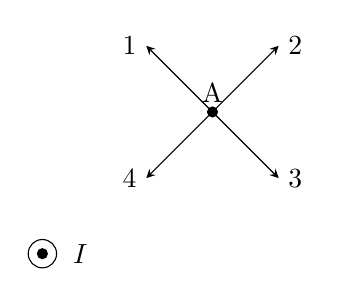
\begin{tikzpicture}[>=stealth, scale=1.2]
  % A nuqtasi
  \filldraw (0,1.5) circle (1.5pt) node[above] {A};
  
  % Yo'nalish vektorlari (X shaklida)
  \draw[->] (0,1.5) -- (-0.7,2.2) node[left] {1};  % Yuqori-chap
  \draw[->] (0,1.5) -- (0.7,2.2) node[right] {2};  % Yuqori-o'ng
  \draw[->] (0,1.5) -- (0.7,0.8) node[right] {3};  % Pastki-o'ng
  \draw[->] (0,1.5) -- (-0.7,0.8) node[left] {4};  % Pastki-chap
  
  % Tok belgisi (biz tomonga chiquvchi)
  \draw (-1.8,0) circle (0.15);
  \filldraw (-1.8,0) circle (1.5pt);
  \node at (-1.4,0) {$I$};
\end{tikzpicture}

\begin{enumerate}[label=\Alph*)]
\item 4.
\item 1.
\item 2.
\item 3.
\end{enumerate}

\item Muhitdagi cheksiz to‘g‘ri $I$ tokning o‘zidan $r$ masofada hosil qiladigan magnit maydon induksiyasining ifodasini ko‘rsating.
\begin{enumerate}[label=\Alph*)]
\item $\frac{\mu\mu_0 I}{2\pi r}$
\item $\frac{\mu\mu_0 I}{4\pi r}$
\item $\frac{\mu\mu_0 U}{4\pi r}$
\item $\frac{2\mu\mu_0 I}{\pi r}$
\end{enumerate}


\item Magnit maydon ikkita parallel va teng toklar tomonidan hosil qilingan (rasmga q.). A nuqtada magnit induksiya vektori qanday yo‘nalgan?

\begin{tikzpicture}[>=stealth, scale=1.5]
  % Gorizontal punktir chiziq
  \draw[dashed] (-2,0) -- (2,0);
  
  % Chapdagi tok (bizga chiquvchi - nuqta)
  \draw[thick] (-1.5,0) circle (0.15);
  \filldraw (-1.5,0) circle (1.5pt);
  \node at (-1.5,0.4) {$I$};
  
  % O'ngdagi tok (ichkariga kiruvchi - krest)
  \draw[thick] (1.5,0) circle (0.15);
  \draw (1.39,0.11) -- (1.61,-0.11);
  \draw (1.39,-0.11) -- (1.61,0.11);
  \node at (1.5,0.4) {$I$};
  
  % Vertikal punktir chiziq va A nuqtasi
  \draw[dashed] (0,0.5) -- (0,-0.8);
  \filldraw (0,-0.6) circle (1.5pt) node[right] {A};
\end{tikzpicture}

\begin{enumerate}[label=\Alph*)]
\item bizga.
\item pastga.
\item yuqoriga.
\item bizdan.
\end{enumerate}

\item Ikkita bir xil kuchli, o‘zaro parallel va ''bizdan`` yo‘nalgan to‘g‘ri chiziqli toklarning hosil qilgan magnit maydon induksiyasi A nuqtada qanday yo‘nalgan?

\begin{tikzpicture}[>=stealth, scale=1.5]
  % Gorizontal punktir chiziq
  \draw[dashed] (-2,0) -- (2,0);
  
  % Chapdagi tok (ichkariga kiruvchi - krest)
  \draw[thick] (-1.5,0) circle (0.15);
  \draw (-1.61,0.11) -- (-1.39,-0.11);
  \draw (-1.61,-0.11) -- (-1.39,0.11);
  \node at (-1.5,0.4) {$I$};
  
  % O'ngdagi tok (ichkariga kiruvchi - krest)
  \draw[thick] (1.5,0) circle (0.15);
  \draw (1.39,0.11) -- (1.61,-0.11);
  \draw (1.39,-0.11) -- (1.61,0.11);
  \node at (1.5,0.4) {$I$};
  
  % Vertikal punktir chiziq va A nuqtasi
  \draw[dashed] (0,0.5) -- (0,-0.8);
  \filldraw (0,-0.6) circle (1.5pt) node[right] {A};
\end{tikzpicture}

\begin{enumerate}[label=\Alph*)]
\item yuqoriga.
\item chapga.
\item nolga teng.
\item pastga.
\end{enumerate}

\item Ikkita bir xil kuchli, o‘zaro parallel va ''bizga`` yo‘nalgan to‘g‘ri chiziqli toklarning hosil qilgan magnit maydon induksiyasi A nuqtada qanday yo‘nalgan?

\begin{tikzpicture}[>=stealth, scale=1.5]
  % Gorizontal punktir chiziq
  \draw[dashed] (-2,0) -- (2,0);
  
  % Chapdagi tok (biz tomonga chiquvchi - nuqta)
  \draw[thick] (-1.5,0) circle (0.15);
  \filldraw (-1.5,0) circle (1.5pt);
  \node at (-1.5,0.4) {$I$};
  
  % O'ngdagi tok (biz tomonga chiquvchi - nuqta)
  \draw[thick] (1.5,0) circle (0.15);
  \filldraw (1.5,0) circle (1.5pt);
  \node at (1.5,0.4) {$I$};
  
  % Vertikal punktir chiziq va A nuqtasi
  \draw[dashed] (0,0.5) -- (0,-0.8);
  \filldraw (0,-0.6) circle (1.5pt) node[right] {A};
\end{tikzpicture}

\begin{enumerate}[label=\Alph*)]
\item o‘ngga.
\item yuqoriga.
\item nolga teng.
\item chapga.
\end{enumerate}

\item Bir-biridan $d$ masofada joylashgan va har biridan bir xil yo‘nalishda $I$ tok o‘tayotgan ikki o‘zaro parallel to‘g‘ri o‘tkazgichlarning o‘rtasidagi nuqtada magnit maydon induksiyasi qanday bo‘ladi?



\begin{enumerate}[label=\Alph*)]
\item $\mu_0 \frac{2I}{\pi d}$
\item $\mu_0 \frac{I}{\pi d}$
\item 0.
\item $\mu_0 \frac{I}{2\pi d}$
\end{enumerate}


\item Rasmda 4 juft tok unsurlari keltirilgan. Qaysi holda ular o‘zaro itarishadi?
\begin{enumerate}[label=\Alph*)]
\item $\uparrow \uparrow$.
\item $\uparrow \rightarrow$.
\item $\rightarrow \leftarrow$.
\item $\downarrow \uparrow$.
\end{enumerate}

\item Ma’lumki, ikkita proton bir-biridan Kulon kuchi vositasida itarishishadi. Qanday holatda ular bir-biriga tortiladi?
\begin{enumerate}[label=\Alph*)]
\item o‘zaro teskari parallel yo‘nalishda o‘ta katta tezlikda harakatlanganda.
\item o‘zaro bir xil yo‘nalishda parallel o‘ta katta tezlikda harakatlanganda.
\item o‘zaro teskari yo‘nalishda bir-biridan uzoqlashsa.
\item hech qachon ular tortishmaydilar.
\end{enumerate}

\item $I_1=10$ A tok o‘tayotgan birinchi o‘tkazgich o‘zidan 10 cm uzoqlikda unga parallel joylashgan ikkinchi o‘tkazgichning har 1 m uzunligini $4 \cdot 10^{-4}$ N kuch bilan itarayotgan bo‘lsa, ikkinchi o‘tkazgichdan o‘tayotgan tok necha Amper va qaysi yo‘nalishda oqmoqda?

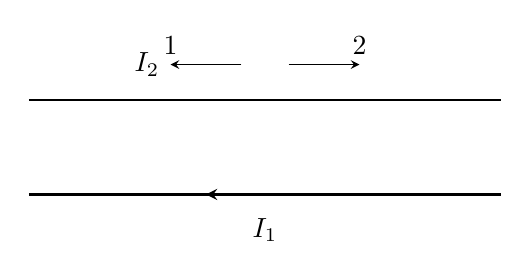
\begin{tikzpicture}[>=stealth, scale=1.5]
  % Pastki o'tkazgich (I1)
  \draw[thick] (-2,0) -- (2,0);
  \draw[->, thick] (0.5,0) -- (-0.5,0);
  \node at (0,-0.3) {$I_1$};
  
  % Yuqorigi o'tkazgich (I2)
  \draw[thick] (-2,0.8) -- (2,0.8);
  \node at (-1,1.1) {$I_2$};
  
  % Yo'nalish ko'rsatkichlari (1 va 2)
  \draw[->] (-0.2,1.1) -- (-0.8,1.1) node[above] {1};
  \draw[->] (0.2,1.1) -- (0.8,1.1) node[above] {2};
\end{tikzpicture}

\begin{enumerate}[label=\Alph*)]
\item 10 A; 1-yo‘nalishda.
\item 20 A; 2-yo‘nalishda.
\item 15 A; 1-yo‘nalishda.
\item 15 A; 2-yo‘nalishda.
\end{enumerate}

\item Keltirilgan ta’riflardan qaysi birida tok kuchi birligi (1 A) to‘g‘ri aniqlangan?
\begin{enumerate}[label=\Alph*)]
\item induktivligi 1 H bo‘lgan g‘altak hosil qilayotgan oqim 1 Wb bo‘lgandagi tok.
\item o‘tkazgich kesimidan 1 s da 1 C zaryad o‘tgandagi tok.
\item qarshiligi 1 $\Omega$ bo‘lgan o‘tkazgichdan o‘tgan tok.
\item vakuumda 1 m masofada parallel o‘tkazgichlar orasidagi $2 \cdot 10^{-7}$ N kuchni vujudga keltiruvchi tok.
\end{enumerate}

\end{enumerate}



\begin{table}[!ht]
\centering
\begin{tabular}{|c|c|c|c|c|c|c|c|}
\hline
1c & 2c & 3d & 4a & 5a & 6b & 7b & 8a \\ \hline
9c & 10b & 11a & 12c & 13d & 14b & 15b & 16d \\ \hline
\end{tabular}
\end{table}









\section{Amper kuchi}



\begin{enumerate}

\item Magnit maydonning tokli o‘tkazgichga ta’sir kuchi (Amper kuchi) ni ifodalaydigan formulani ko‘rsating.
\begin{enumerate}[label=\Alph*)]
\item $F = IBL\cos\alpha$.
\item $F = kq_1q_2/r^2$.
\item $F = Eq$.
\item $F = IBL\sin\alpha$.
\end{enumerate}

\item Induksiyasi 20 T bo‘lgan bir jinsli magnit maydonda 3 A tok o‘tayotgan o‘tkazgich rasmdagidek joylashgan. Unga ta’sir qilayotgan Amper kuchining modulini toping (N). O‘tkazgichning aktiv qismining uzunligi 40 cm. $\alpha=37^\circ$.

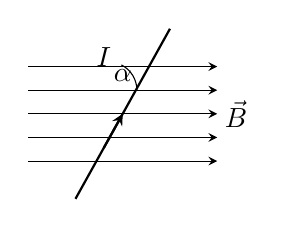
\begin{tikzpicture}[>=stealth, scale=1.2]
  % Magnit maydon induksiya chiziqlari (B)
  \foreach \y in {0, 0.25, 0.5, 0.75, 1.0} {
    \draw[->, thin] (-1, \y) -- (1, \y);
  }
  \node at (1.2, 0.5) {$\vec{B}$};
  
  % Tokli o'tkazgich
  \draw[thick] (-0.5, -0.4) -- (0.5, 1.4);
  \draw[->, thick] (-0.2, 0.14) -- (0, 0.5); % Tok yo'nalishi ko'rsatkichi
  \node at (-0.2, 1.1) {$I$};
  
  % Alfa burchagi
  \draw (0.15, 0.75) arc (0:63:0.3);
  \node at (0, 0.9) {$\alpha$};
\end{tikzpicture}

\begin{enumerate}[label=\Alph*)]
\item 14,4.
\item 12,8.
\item 10,2.
\item 16,4.
\end{enumerate}

\item Induksiyasi 2 T bo‘lgan bir jinsli magnit maydonga kiritilgan 8 cm uzunlikdagi o‘tkazgichdan 4 A tok oqayotgan bo‘lsa, bu o‘tkazgichga maydon tomonidan qanday kuch ta’sir qiladi (N)? Tok va magnit induksiya vektori orasidagi burchak $30^\circ$ ga teng.
\begin{enumerate}[label=\Alph*)]
\item 0,4.
\item 0,24.
\item 0,32.
\item 1,25.
\end{enumerate}

\item Aktiv qismining uzunligi 0,4 m bo‘lgan o‘tkazgich induksiyasi 0,8 T bo‘lgan bir jinsli magnit maydoniga kiritilganda unga 1,6 N kuch ta’sir etdi. O‘tkazgich magnit induksiya chiziqlariga perpendikulyar joylashgan bo‘lsa, undagi tok kuchini aniqlang (A).
\begin{enumerate}[label=\Alph*)]
\item 5.
\item 4.
\item 3.
\item 2.
\end{enumerate}

\item Induksiyasi 40 mT bo‘lgan magnit maydon aktiv qismining uzunligi 10 cm bo‘lgan to‘g‘ri o‘tkazgichga 60 mN kuch bilan ta’sir etmoqda. O‘tkazgichdagi tok kuchi 30 A. O‘tkazgich magnit maydon induksiyasi vektori bilan qanday burchak hosil qiladi?
\begin{enumerate}[label=\Alph*)]
\item $90^\circ$.
\item $60^\circ$.
\item $45^\circ$.
\item $30^\circ$.
\end{enumerate}

\setcounter{enumi}{5}
\item Induksiyasi 2 T bo‘lgan bir jinsli magnit maydonda uzunligi 0,2 m bo‘lgan o‘tkazgich joylashgan. Agar o‘tkazgichdan o‘tayotgan o‘zgarmas tok kuchi 5 A bo‘lsa, magnit maydon tomonidan o‘tkazgichga ta’sir etuvchi maksimal va minimal kuchlar nimaga teng bo‘lishi mumkin (N)?
\begin{enumerate}[label=\Alph*)]
\item 2; 0.
\item 2; 1.
\item 10; 2.
\item 1; 0.
\end{enumerate}

\item Vakuumda magnit kuchlanganligi $H=5000$ A/m bo‘lgan magnit maydon hosil qilindi. U yerga uzunligi 20 cm bo‘lgan va 10 A tok o‘tayotgan o‘tkazgich joylashtirildi. Tok va magnit induksiyasi yo‘nalishlari o‘zaro $53^\circ$ burchak hosil qilsa, Amper kuchi qanday (mN) bo‘ladi? $\sin 53^\circ = 0,8$, $\pi=3$.
\begin{enumerate}[label=\Alph*)]
\item 9,6.
\item 2.
\item 2,3.
\item 4,5.
\end{enumerate}

\item Induksiyasi 5 T bo‘lgan magnit maydonda uzunligi 20 cm bo‘lgan o‘tkazgich bo‘lib, undan 10 A tok o‘tmoqda. Agar o‘tkazgich magnit induksiyasi yo‘nalishi bilan $30^\circ$ burchak hosil qilsa, unga maydon tomonidan necha Nyuton kuch ta’sir qiladi?
\begin{enumerate}[label=\Alph*)]
\item 10.
\item 1,5.
\item 5.
\item 18.
\end{enumerate}

\item Magnit induksiya chiziqlariga tik joylashgan tokli o‘tkazgichga 2,8 N kuch ta’sir etmoqda. O‘tkazgich bilan induksiya chiziqlari orasidagi burchak $30^\circ$ bo‘lganda, ta’sir kuchi qanday bo‘ladi (N)?
\begin{enumerate}[label=\Alph*)]
\item 0,7.
\item 1,4.
\item 1,96.
\item 2,4.
\end{enumerate}

\item Bir jinsli magnit maydon induksiyasi vektori va tokli to‘g‘ri o‘tkazgich orasidagi $30^\circ$ burchak 2 marta orttirilsa, o‘tkazgichga ta’sir qiluvchi Amper kuchi qanday o‘zgaradi?
\begin{enumerate}[label=\Alph*)]
\item 2 marta ortadi.
\item 2 marta kamayadi.
\item $\sqrt{2}$ marta ortadi.
\item $\sqrt{3}$ marta ortadi.
\end{enumerate}

\setcounter{enumi}{10}
\item Aktiv qismining uzunligi 10 cm bo‘lgan o‘tkazgichdagi tok kuchi 2 A ga teng. U magnit induksiyasi 0,08 T bo‘lgan bir jinsli magnit maydonda turibdi. O‘tkazgich induksiya chiziqlariga perpendikulyar ravishda 10 cm siljiganda necha mJ ish bajariladi?
\begin{enumerate}[label=\Alph*)]
\item 32.
\item 0,8.
\item 3,2.
\item 1,6.
\end{enumerate}

\item Induksiyasi 20 mT bo‘lgan bir jinsli magnit maydon chiziqlariga tik joylashgan 8 cm uzunlikdagi simdan 50 A tok oqmoqda. Bu sim o‘ziga tik yo‘nalishda induksiya chiziqlariga $45^\circ$ burchak ostida ko‘chganida tok 8 mJ ish bajargan bo‘lsa, sim qanday (cm) masofaga ko‘chgan?
\begin{enumerate}[label=\Alph*)]
\item 10,2.
\item 13,2.
\item 14,1.
\item 15,2.
\end{enumerate}

\item Uzunligi 0,1 m bo‘lgan 5 A tokli o‘tkazgichni bir jinsli magnit maydonda induksiya chiziqlariga va o‘ziga tik yo‘nalishda 20 mm masofaga siljitishda 0,01 J ish bajariladi. Magnit maydon induksiyasi necha Tesla?
\begin{enumerate}[label=\Alph*)]
\item 0,1.
\item 1.
\item 2.
\item 0,2.
\end{enumerate}

\item Uzunligi 20 cm bo‘lgan 2 A tokli o‘tkazgich bir jinsli magnit maydon induksiya chiziqlariga perpendikulyar yo‘nalishda 10 cm siljiganda, 32 mJ ish bajarildi. Magnit maydon induksiyasini toping (T).
\begin{enumerate}[label=\Alph*)]
\item 0,04.
\item 0,08.
\item 0,4.
\item 0,8.
\end{enumerate}

\item Uzunligi 80 cm bo‘lgan o‘tkazgich induksiyasi 0,4 T bo‘lgan bir jinsli magnit maydonda 0,15 m/s tezlik bilan induksiya chiziqlariga va o‘ziga tik yo‘nalishda tekis harakat qilmoqda. Agar 10 s ichida 0,96 J ish bajarilgan bo‘lsa, o‘tkazgichdagi tok kuchi qanday (A) bo‘ladi?
\begin{enumerate}[label=\Alph*)]
\item 0,4.
\item 1.
\item 2.
\item 1,8.
\end{enumerate}

\item Yuzi $S=1,2$ m$^2$ bo‘lgan 2 A tokli ramka induksiyasi 30 T bo‘lgan bir jinsli magnit maydonda joylashgan. Ramka normali va induksiya chiziqlari orasidagi burchak $53^\circ$ ga teng. Ramkaga ta’sir qiluvchi kuch momenti nimaga teng (N$\cdot$m)?
\begin{enumerate}[label=\Alph*)]
\item 16,8.
\item 64,2.
\item 57,6.
\item 28,5.
\end{enumerate}

\end{enumerate}




\begin{table}[!ht]
\centering
\begin{tabular}{|c|c|c|c|c|c|c|c|}
\hline
1d & 2a & 3c & 4a & 5d & 6a & 7a & 8c \\ \hline
9b & 10d & 11d & 12c & 13b & 14d & 15c & 16c \\ \hline
\end{tabular}
\end{table}












\section{Lorens kuchi}



\begin{enumerate}

\item Quyidagilar ichidan Lorens kuchining ifodasini toping.
\begin{enumerate}[label=\Alph*)]
\item $qvB\sin\alpha$.
\item $qvB\cos\alpha$.
\item $vB/2$.
\item $vB\sin\alpha$.
\end{enumerate}

\item Induksiyasi 20 T bo‘lgan magnit maydonga 0,2 C zaryadga ega zarra 25 m/s tezlik bilan induksiya chiziqlariga $53^\circ$ burchak ostida uchib kirdi. Unga ta’sir qilayotgan Lorens kuchini toping (N).
\begin{enumerate}[label=\Alph*)]
\item 100.
\item 20.
\item 30.
\item 80.
\end{enumerate}

\item Induksiyasi 4 T bo‘lgan bir jinsli magnit maydonga $10^7$ m/s tezlik bilan induksiya chiziqlariga perpendikulyar yo‘nalishda uchib kirgan elektronga ta’sir etuvchi kuchning moduli qanday (N)? $e = -1,6 \cdot 10^{-19}$ C.
\begin{enumerate}[label=\Alph*)]
\item $6,4 \cdot 10^{-12}$.
\item $0,4 \cdot 10^{-7}$.
\item $0,14 \cdot 10^{-12}$.
\item $3,2 \cdot 10^{-12}$.
\end{enumerate}

\item Induksiyasi 0,2 T bo‘lgan magnit maydonda induksiya chiziqlariga tik ravishda 10 Mm/s tezlik bilan harakatlanayotgan protonga qanday kuch ta’sir qiladi (pN). $e = 1,6 \cdot 10^{-19}$ C.
\begin{enumerate}[label=\Alph*)]
\item 0,5.
\item 0,16.
\item 0,32.
\item 0,64.
\end{enumerate}

\item Magnit kuch chiziqlariga tik yo‘nalishda 2 km/s tezlik bilan harakatlanayotgan 0,4 C zaryadga ta’sir qilayotgan Lorens kuchi 8 N ga teng bo‘lsa, magnit induksiyasi qanday?
\begin{enumerate}[label=\Alph*)]
\item 10 mT.
\item 10 T.
\item 1,6 mT.
\item 1,6 T.
\end{enumerate}

\item Induksiyasi 0,2 T bo‘lgan magnit maydonga induksiya chiziqlariga tik ravishda elektron uchib kirdi. Unga ta’sir etuvchi kuch $0,32 \cdot 10^{-12}$ N bo‘lsa, uning tezligi qanday (m/s)? $e = 1,6 \cdot 10^{-19}$ C.
\begin{enumerate}[label=\Alph*)]
\item $1,6 \cdot 10^5$.
\item $1 \cdot 10^7$.
\item $32 \cdot 10^5$.
\item $6,4 \cdot 10^4$.
\end{enumerate}

\item Protonning tezligi 24 marta kamayganda va magnit maydon induksiyasi 12 marta ortganda, magnit maydon tomonidan protonga ta’sir qiluvchi Lorens kuchi qanday o‘zgaradi?
\begin{enumerate}[label=\Alph*)]
\item 2 marta ortadi.
\item 4 marta kamayadi.
\item 4 marta ortadi.
\item 2 marta kamayadi.
\end{enumerate}


\item Magnit maydonda harakatlanayotgan manfiy zaryadlangan zarrachaga ta’sir etuvchi Lorens kuchi yo‘nalishi chizmada ko‘rsatilgan qaysi yo‘nalish bilan mos tushadi? Magnit maydon kuch chiziqlarari bizdan chizma tekisligiga tik yo‘nalgan.

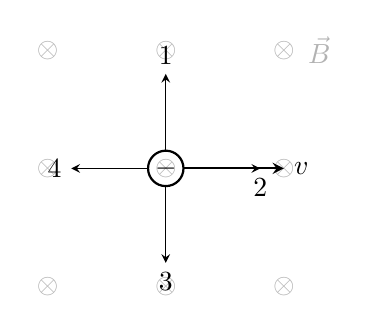
\begin{tikzpicture}[>=stealth, scale=1.5]
  % Magnit maydon induksiyasi (krestlar - bizdan ichkariga)
  \foreach \x in {-1, 0, 1} {
    \foreach \y in {-1, 0, 1} {
      \node[gray!60] at (\x, \y) {$\otimes$};
    }
  }
  \node[gray!60] at (1.3, 1) {$\vec{B}$};

  % Markaziy manfiy zaryad
  \draw[thick] (0,0) circle (0.15);
  \node at (0,0) {$-$};
  
  % Tezlik vektori (v)
  \draw[->, thick] (0.15,0) -- (1,0) node[right] {$v$};
  
  % Yo'nalish ko'rsatkichlari (1, 2, 3, 4)
  \draw[->] (0, 0.15) -- (0, 0.8) node[above] {1}; % Yuqoriga
  \draw[->] (0.5, 0) -- (0.8, 0) node[below] {2};  % O'ngga
  \draw[->] (0, -0.15) -- (0, -0.8) node[below] {3}; % Pastga
  \draw[->] (-0.15, 0) -- (-0.8, 0) node[left] {4}; % Chapga
\end{tikzpicture}

\begin{enumerate}[label=\Alph*)]
\item 1.
\item 3.
\item 4.
\item 2.
\end{enumerate}

\item Harakatlanayotgan musbat zaryadli zarraga magnit maydon tomonidan ta’sir etadigan Lorens kuchining yo‘nalishini aniqlang. Maydonning magnit induksiyasi vektori chizma tekisligiga tik va bizdan chizmaga tomon yo‘nalgan ($\otimes$).

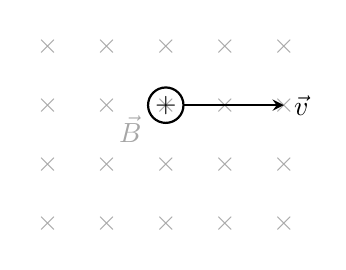
\begin{tikzpicture}[>=stealth, scale=1.5]
  % Magnit maydon induksiyasi (krestlar - bizdan ichkariga)
  \foreach \x in {-1, -0.5, 0, 0.5, 1} {
    \foreach \y in {-0.5, 0, 0.5, 1} {
      \node[gray!70] at (\x, \y) {$\times$};
    }
  }
  \node[gray!70] at (-0.3, 0.3) {$\vec{B}$};

  % Markaziy musbat zaryad
  \draw[thick] (0,0.5) circle (0.15);
  \node at (0,0.5) {$+$};
  
  % Tezlik vektori (v)
  \draw[->, thick] (0.15,0.5) -- (1,0.5) node[right] {$\vec{v}$};
  
 \end{tikzpicture}

\begin{enumerate}[label=\Alph*)]
\item o‘ngga.
\item pastga.
\item yuqoriga.
\item chapga.
\end{enumerate}

\item Elektron rasmda ko‘rsatilganidek, bir jinsli magnit maydoniga uchib kiradi. Unga magnit maydoni tomonidan ta’sir qiladigan kuch qaysi tomonga yo‘naladi?

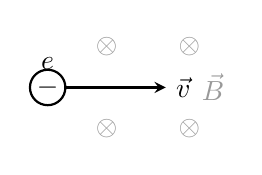
\begin{tikzpicture}[>=stealth, scale=1.5]
  % Magnit maydon induksiyasi (krestlar - bizdan ichkariga)
  \foreach \x in {0.5, 1.2} {
    \foreach \y in {0, 0.7} {
      \node[gray!80] at (\x, \y) {$\otimes$};
    }
  }
  \node[gray!80] at (1.4, 0.35) {$\vec{B}$};

  % Elektron (e)
  \draw[thick] (0,0.35) circle (0.15);
  \node at (0,0.55) {$e$};
  \node at (0,0.35) {$-$};
  
  % Tezlik vektori (v)
  \draw[->, thick] (0.15,0.35) -- (1,0.35) node[right] {$\vec{v}$};
  
  
\end{tikzpicture}

\begin{enumerate}[label=\Alph*)]
\item o‘ngga.
\item pastga.
\item yuqoriga.
\item chapga.
\end{enumerate}


\item Tezligi $v$ bo‘lgan $q$ zaryad induksiyasi $B$ bo‘lgan magnit maydonga kuch chiziqlariga tik ravishda uchib kirdi. Shu zaryad harakat traektoryasining egrilik radiusi qaysi ifoda asosida hisoblanishi mumkin?
\begin{enumerate}[label=\Alph*)]
\item $mv/qB$.
\item $qv/mB$.
\item $qB/mv$.
\item $vB/qm$.
\end{enumerate}

\item Tezligi $v$ va zaryadi $q$ bo‘lgan ion induksiyasi $B$ bo‘lgan bir jinsli magnit maydonga kiradi va $R$ radiusli aylana chizadi. Ionning massasi qanday ifoda vositasida hisoblanadi?
\begin{enumerate}[label=\Alph*)]
\item $qvB/R$.
\item $qvR/B$.
\item $qBR/v$.
\item $B/qvR$.
\end{enumerate}

\item Induksiyasi 20 T bo‘lgan magnit maydonga 0,08 g massali 0,002 C zaryadga ega zarra 25 m/s tezlik bilan induksiya chiziqlariga tik ravishda uchib kirdi. Uning aylanish radiusini (cm) va aylanish davrini (ms) toping.
\begin{enumerate}[label=\Alph*)]
\item 5; 4,76.
\item 8; 12,56.
\item 4; 4,76.
\item 5; 12,56.
\end{enumerate}

\item Induksiyasi 9,1 mT bo‘lgan bir jinsli magnit maydonga induksiya chiziqlariga perpendikulyar ravishda 16 Mm/s tezlik bilan uchib kirgan elektron harakat traektoryasining egrilik radiusini toping (cm). $m = 9,1 \cdot 10^{-31}$ kg, $e = 1,6 \cdot 10^{-19}$ C.
\begin{enumerate}[label=\Alph*)]
\item 100.
\item 10.
\item 0,1.
\item 1.
\end{enumerate}

\item Elektron induksiyasi 5 mT bo‘lgan magnit maydonga uchib kirib, 4 cm radiusli aylana bo‘ylab harakatlana boshlasa, uning tezligi qanday (m/s)?
\begin{enumerate}[label=\Alph*)]
\item $6 \cdot 10^6$.
\item 1000.
\item $3,5 \cdot 10^7$.
\item $5 \cdot 10^7$.
\end{enumerate}

\item Proton induksiyasi 20 mT bo‘lgan bir jinsli magnit maydonda 5 cm radiusli aylana chizdi. Proton zaryadi $1,6 \cdot 10^{-19}$ C bo‘lsa, uning impulsini aniqlang (kg$\cdot$m/s).
\begin{enumerate}[label=\Alph*)]
\item $3,2 \cdot 10^{-20}$.
\item $5 \cdot 10^{-21}$.
\item $1,6 \cdot 10^{-22}$.
\item $8 \cdot 10^{-22}$.
\end{enumerate}

\item Bir xil tezlikka ega bo‘lgan ikkita bir xil zaryadlangan zarralar magnit maydonga kuch chiziqlariga tik yo‘nalishda kirib, egrilik radiuslari $R_2 = 3R_1$ munosabatda bo‘lgan traektoriya bo‘yicha harakat qila boshladilar. 2-zarra massasi $m_2$ ning 1-zarra massasi $m_1$ ga nisbati $m_2/m_1$ qanday?
\begin{enumerate}[label=\Alph*)]
\item 0,5.
\item 1/3.
\item 2.
\item 3.
\end{enumerate}


\item Massasi $m$, zaryadi $q$ bo‘lgan zarracha induksiyasi $B$ bo‘lgan bir jinsli magnit maydonda aylana bo‘ylab harakatlanmoqda. Aylanish davrini toping.
\begin{enumerate}[label=\Alph*)]
\item $\pi m / 2qB$.
\item $\pi m / qB$.
\item $2\pi m / qB$.
\item $2\pi r^2 / v$.
\end{enumerate}

\item Agar bir jinsli magnit maydonda elektronning aylanish davri 9 ns bo‘lsa magnit maydon induksiyasi necha mT bo‘ladi? Elektronning zaryadi $1,6 \cdot 10^{-19}$ C, massasi $9,1 \cdot 10^{-31}$ kg.
\begin{enumerate}[label=\Alph*)]
\item 4,5.
\item 8.
\item 9.
\item 4.
\end{enumerate}

\item Induksiyasi 16,7 mT bo‘lgan bir jinsli magnit maydonga induksiya chiziqlariga tik yo‘nalishda uchib kirgan proton aylana traektoriya bo‘ylab harakatlanadi. Protonning 3,14 s ichidagi aylanishlar sonini toping. $e = 1,6 \cdot 10^{-19}$ C, $m_p = 1,67 \cdot 10^{-27}$ kg.
\begin{enumerate}[label=\Alph*)]
\item $4 \cdot 10^5$.
\item $8 \cdot 10^5$.
\item $3 \cdot 10^6$.
\item $6 \cdot 10^6$.
\end{enumerate}

\item Magnit induksiyasi 16,7 mT bo‘lgan bir jinsli magnit maydoniga induksiya chiziqlariga tik yo‘nalishda uchib kirgan proton aylana traektoriya bo‘ylab harakatlanadi. $6\pi$ s ichida protonning aylanishlar soni qanchaga teng bo‘ladi?
\begin{enumerate}[label=\Alph*)]
\item $6,2 \cdot 10^5$.
\item $4 \cdot 10^5$.
\item $6,2 \cdot 10^6$.
\item $4,8 \cdot 10^6$.
\end{enumerate}

\end{enumerate}




\begin{table}[!ht]
\centering
\begin{tabular}{|c|c|c|c|c|c|c|c|c|c|c|}
\hline
1a & 2d & 3a & 4c & 5a & 6b & 7d & 8b & 9c & 10b & 11a \\ \hline
12c & 13d & 14d & 15c & 16c & 17d & 18c & 19d & 20b & 21d & \\ \hline
\end{tabular}
\end{table}












\section{Magnit oqimi}


\begin{enumerate}

\item O‘lchov birliklarining xalqaro sistemasida magnit oqimining birligi qanday?
\begin{enumerate}[label=\Alph*)]
\item Kulon.
\item Tesla.
\item Veber.
\item Amper.
\end{enumerate}

\item Radiusi $r=20$ cm bo‘lgan xalqa induksiyasi $B=0,3$ T bo‘lgan bir jinsli magnit maydonda joylashgan. Induksiya vektori xalqa normali bilan $\alpha=37^\circ$ burchak hosil qiladi. Xalqani kesib o‘tuvchi magnit oqimini toping (mWb). $\pi=3$.

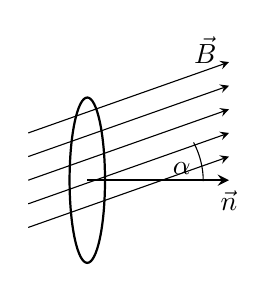
\begin{tikzpicture}[>=stealth, scale=1.5]
  % Xalqa (perspektivada ellips ko'rinishida)
  \draw[thick] (0,0) ellipse (0.15 and 0.7);
  
  % Magnit maydon chiziqlari (B) - tepaga va o'ngga yo'nalgan
  \foreach \i in {-2,-1,0,1,2} {
    \draw[->, thin] (-0.5, 0.2*\i) -- (1.2, 0.2*\i + 0.6);
  }
  \node at (1.0, 1.1) {$\vec{B}$};
  
  % Normal vektor (n) - sirtga tik, pastga va o'ngga yo'nalgan
  \draw[->, thick] (0,0) -- (1.2, 0) node[below] {$\vec{n}$};
  
  % Alfa burchagi (n va B chiziqlari orasida)
  \draw (0.9, 0.32) arc (28:0:0.7);
  \node at (0.8, 0.1) {$\alpha$};
\end{tikzpicture}

\begin{enumerate}[label=\Alph*)]
\item 3,14.
\item 10.
\item 28,8.
\item 15.
\end{enumerate}

\item Yuzi 0,2 m$^2$ bo‘lgan kontur induksiyasi 5 T bo‘lgan bir jinsli magnit maydonda joylashgan. Agar kontur tekisligi induksiya chiziqlariga parallel joylashgan bo‘lsa, kontur yuzidan o‘tayotgan magnit oqimi necha Veber bo‘ladi?
\begin{enumerate}[label=\Alph*)]
\item 0.
\item 0,1.
\item 0,5.
\item 1.
\end{enumerate}

\item To‘g‘ri to‘rtburchak shaklidagi ramkani induksiyasi 6,5 T bo‘lgan magnit maydon rasmdagi kabi kesib o‘tmoqda. Unga tushayotgan magnit oqimini toping (Wb).


\begin{tikzpicture}[>=stealth, x={(1.2cm,0cm)}, y={(0cm,1.2cm)}, z={(-0.6cm,-0.4cm)}, scale=1.8]
  % Koordinata o'qlari
  \draw[->] (0,0,0) -- (1.8,0,0) node[right] {x};
  \draw[->] (0,0,0) -- (0,1.3,0) node[above] {y};
  \draw[->] (0,0,0) -- (0,0,1.8) node[below left] {z};
  
  % To'g'ri to'rtburchakli ramka (yz-tekisligida)
  \draw[thick] (0,0,0) -- (0,1,0) -- (0,1,1.5) -- (0,0,1.5) -- cycle;
  
  % O'lchamlar va yozuvlar
  \node[left, rotate=90] at (0,1,0) {20 cm};
  \node[below, sloped] at (0,0,1.5) {40 cm};
  
  % Magnit induksiya vektori (B)
  \draw[->, very thick] (0,0.5,0.75) -- (1.5,0.5,0.75) node[right] {$\vec{B}$};
  
  % Perpendikulyarlik belgilari (B vektori y va z o'qlariga tikligini ko'rsatadi)
  \draw (0.15,0.5,0.75) -- (0.15,0.65,0.75) -- (0,0.65,0.75);
 
\end{tikzpicture}

\begin{enumerate}[label=\Alph*)]
\item 0,52.
\item 0,27.
\item 0,39.
\item 0,48.
\end{enumerate}

\item Radiusi 5 cm bo‘lgan doirasimon yuza induksiyasi 2 T bo‘lgan bir jinsli magnit maydonda joylashgan. Induksiya vektori doira sirti normali bilan $0^\circ$ burchak hosil qiladi. Sirtni kesib o‘tuvchi magnit oqimini toping (mWb).
\begin{enumerate}[label=\Alph*)]
\item 3,14.
\item 10.
\item 30,5.
\item 15,7.
\end{enumerate}

\item Tomonlari 4 cm dan bo‘lgan teng tomonli uchburchak induksiyasi 2 T bo‘lgan bir jinsli magnit maydonda joylashgan. Induksiya vektori uchburchak sirti normali bilan $30^\circ$ burchak hosil qiladi. Sirtni kesib o‘tuvchi magnit oqimini toping (mWb). 
\begin{enumerate}[label=\Alph*)]
\item $0,8\sqrt{3}$.
\item $0,4\sqrt{3}$.
\item $0,4\sqrt{6}$.
\item 1,2.
\end{enumerate}

\item Yuzi 2 m$^2$ bo‘lgan va magnit maydon induksiyasi vektoriga tik joylashgan yassi konturdan 10 Wb magnit oqim o‘tsa, magnit induksiyasi qanday (T)?
\begin{enumerate}[label=\Alph*)]
\item 0,2.
\item 0,4.
\item 2,5.
\item 5.
\end{enumerate}

\item Magnit maydon induksiyasi vektoriga tik bo‘lgan yassi konturdan 6 Wb magnit oqim o‘tadi. Agar magnit induksiyasi 3 T bo‘lsa, konturning yuzi qanday (m$^2$)?
\begin{enumerate}[label=\Alph*)]
\item 0,5.
\item 2/3.
\item 2.
\item 12.
\end{enumerate}

\item Magnit induksiyasi 4 T bo‘lgan maydonda joylashgan 1 cm radiusli xalqani kesib o‘tayotgan magnit oqim 0,628 mWb bo‘lishi uchun magnit induksiya vektori bilan halqa tekisligi orasidagi burchak qanday bo‘lishi kerak?
\begin{enumerate}[label=\Alph*)]
\item $0^\circ$.
\item $30^\circ$.
\item $45^\circ$.
\item $60^\circ$.
\end{enumerate}

\item Magnit maydon oqimi ortadi, agar ...
1) magnit maydon induksiyasi ortsa;
2) magnit maydon induksiyasi kamaysa;
3) magnit maydon kesib o‘tuvchi yuza kamaysa;
4) magnit maydon kesib o‘tuvchi yuza ortsa.
\begin{enumerate}[label=\Alph*)]
\item 2, 3.
\item 1, 3.
\item 1, 4.
\item 2, 4.
\end{enumerate}

\item Quyidagi hollarning qaysi birida ramka yuzasidan o‘tuvchi magnit induksiya oqimi o‘zgarmaydi? 
\begin{enumerate}[label=\Alph*)]
\item bir jinsli magnit maydonda o‘z tekisligidan o‘tuvchi o‘q atrofida aylanganida.
\item bir jinsli bo‘lmagan magnit maydonda ilgarilanma harakat qilganida.
\item bir jinsli bo‘lmagan magnit maydonda aylanganida.
\item bir jinsli magnit maydonda ilgarilanma harakat qilganida.
\end{enumerate}

\item Yuzi 25 cm$^2$ bo‘lgan sim ramka bir jinsli magnit maydonda aylantirilganda, ramkani kesib o‘tuvchi magnit oqim $\Phi=2,5 \cdot 10^{-4}\cos 6t$ (Wb) qonun bo‘yicha o‘zgaradi. Magnit maydon induksiyasi qanday (T)? 
\begin{enumerate}[label=\Alph*)]
\item 0,1.
\item 0,6.
\item 1.
\item 0,2.
\end{enumerate}

\item Magnit maydonda harakatlanayotgan 5 A tokli kontur bilan chegaralangan yuzadan o‘tuvchi magnit oqim 0,4 mWb dan 0,8 mWb ga o‘zgargan bo‘lsa, necha milliJoul ish bajarilgan?
\begin{enumerate}[label=\Alph*)]
\item 2.
\item 3.
\item 1.
\item 4.
\end{enumerate}

\item Induksiyasi $4/\pi$ T bo‘lgan bir jinsli magnit maydonda diametri 10 cm bo‘lgan va 1 A tok o‘tayotgan o‘ram bor. O‘ramning tekisligi magnit induksiya vektoriga parallel. O‘ramni uning tekisligi magnit induksiya vektoriga tik bo‘ladigan qilib $90^\circ$ ga burish uchun necha Joul ish bajarish kerak? 
\begin{enumerate}[label=\Alph*)]
\item $10^{-2}$.
\item $\pi \cdot 10^{-4}$.
\item $10^{-4}$.
\item $\pi \cdot 10^{-2}$.
\end{enumerate}

\end{enumerate}



\begin{table}[!ht]
\centering
\begin{tabular}{|c|c|c|c|c|c|c|c|c|c|c|}
\hline
1c & 2c & 3a & 4a & 5d & 6d & 7d & 8c & 9b & 10c & 11d \\ \hline
12a & 13a & 14a & & & & & & & & \\ \hline
\end{tabular}
\end{table}



\section{Elektromagnit induksiya qonuni.  Lens qoidasi.}





\begin{enumerate}

\item Faradeyning elektromagnit induksiya qonunining matematik ifodasini toping.
\begin{enumerate}[label=\Alph*)]
\item $\varepsilon=-kF/I$.
\item $\varepsilon=\dfrac{\Delta \Phi}{\Delta t}$.
\item $\varepsilon=-\dfrac{\Delta \Phi}{\Delta t}$.
\item $\varepsilon=k\dfrac{\Delta I}{\Delta \Phi \Delta t}$.
\item $\varepsilon=\dfrac{4\pi\varepsilon_0}{\Delta t}$.
\end{enumerate}

\item Induksiya EYK ning birligini ko‘rsating.
\begin{enumerate}[label=\Alph*)]
\item T/s.
\item B$\cdot$s.
\item Wb/s.
\item T$\cdot$m$^2$.
\item Wb$\cdot$s.
\end{enumerate}

\item Kuchlanish birligi Voltning o‘rniga yana qaysi birlikni ishlatsa bo‘ladi?
\begin{enumerate}[label=\Alph*)]
\item H/s.
\item Wb.
\item Wb/s.
\item H$\cdot$s.
\item Wb$\cdot$s.
\end{enumerate}

\item Berk kontur bir jinsli magnit maydonda induksiya chiziqlari bo‘ylab tezlanish bilan ilgarilanma harakat qilsa, induksiya EYK hosil bo‘ladimi?
\begin{enumerate}[label=\Alph*)]
\item bo‘ladi.
\item bo‘lmaydi.
\item bo‘ladi va chiziqli ravishda kamayib boradi.
\item bo‘ladi va chiziqli ravishda ortib boradi.
\item bo‘ladi va eksponensial ravishda o‘zgaradi.
\end{enumerate}

\item Konturda hosil bo‘luvchi induksiya EYK $50$ V bo‘lishi uchun konturni kesib o‘tuvchi magnit oqimning o‘zgarish tezligi qanday (Wb/s) bo‘lishi kerak?
\begin{enumerate}[label=\Alph*)]
\item 5.
\item 10.
\item 50.
\item 100.
\item 500.
\end{enumerate}

\item Kontur kesib o‘tuvchi magnit oqim $2$ s da $10$ Wb dan $2$ Wb gacha tekis kamaydi. Konturda hosil bo‘lgan induksiya EYK ni toping (V).
\begin{enumerate}[label=\Alph*)]
\item 10.
\item 8.
\item 4.
\item 2.
\item 0.
\end{enumerate}

\item Konturdan o‘tayotgan magnit oqim $0,3$ s davomida $9$ Wb dan $6$ Wb gacha tekis kamaygan bo‘lsa, konturda hosil bo‘lgan induksiya EYK necha Voltga teng?
\begin{enumerate}[label=\Alph*)]
\item 0,01.
\item 0,9.
\item 4,5.
\item 10.
\item 50.
\end{enumerate}

\item Berk kontur kesib o‘tuvchi magnit oqim $0,4$ s davomida $4\cdot10^{-5}$ Wb ga o‘zgardi. Induksiya EYK ni (V) aniqlang.
\begin{enumerate}[label=\Alph*)]
\item $4\cdot10^{-4}$.
\item $10^{-5}$.
\item $10^{-4}$.
\item $4\cdot10^{-5}$.
\item $2\cdot10^{-4}$.
\end{enumerate}

\item Solenoiddagi o‘ramlar soni $2,5$ marta ortsa, undagi induksiya EYK qanday o‘zgaradi?
\begin{enumerate}[label=\Alph*)]
\item o‘zgarmaydi.
\item 5 marta ortadi.
\item 5 marta kamayadi.
\item 2,5 marta ortadi.
\item 2,5 marta kamayadi.
\end{enumerate}

\item $200$ o‘ramga ega bo‘lgan g‘altak ichida magnit oqim $0,2$ s da $0,2$ Wb dan $1,1$ Wb gacha ortdi. G‘altakda induksiyalanadigan EYK ni aniqlang (V).
\begin{enumerate}[label=\Alph*)]
\item 1000.
\item 500.
\item 900.
\item 450.
\item 700.
\end{enumerate}

\item $100$ ta o‘ramdan iborat solenoiddagi magnit maydon oqimi $1$ ms davomida $5\cdot10^{-5}$ Wb dan $15\cdot10^{-5}$ Wb gacha o‘zgarsa, unda vujudga keluvchi induksion EYK necha Volt bo‘ladi?
\begin{enumerate}[label=\Alph*)]
\item 100.
\item 10.
\item 1.
\item 0,1.
\item 0,01.
\end{enumerate}

\item Magnit oqimning o‘zgarish tezligi $0,24$ Wb/s bo‘lganda, g‘altakda $48$ V elektr yurituvchi kuch hosil bo‘lsa, g‘altakdagi o‘ramlar soni qanday?
\begin{enumerate}[label=\Alph*)]
\item 200.
\item 250.
\item 260.
\item 300.
\item 20.
\end{enumerate}

\item Agar magnit oqimning o‘zgarish tezligi $60$ mWb/s bo‘lganda g‘altakda uyg‘onuvchi EYK $\varepsilon=12$ V bo‘lsa, g‘altakdagi o‘ramlar soni qanday?
\begin{enumerate}[label=\Alph*)]
\item 2000.
\item 3000.
\item 2500.
\item 300.
\item 200.
\end{enumerate}

\item Solenoiddagi magnit oqim $2$ ms da $3$ mWb dan $9$ mWb gacha o‘zgargan. Agar solenoidda hosil bo‘lgan EYK $60$ V bo‘lsa, solenoiddagi o‘ramlar soni qanday?
\begin{enumerate}[label=\Alph*)]
\item 5.
\item 20.
\item 180.
\item 200.
\item 300.
\end{enumerate}

\item O‘ramlar soni $80$ ta bo‘lgan tokli g‘altakda induksiya EYK $60$ V bo‘lsa, magnit oqimining o‘zgarish tezligi qanday (Wb/s)?
\begin{enumerate}[label=\Alph*)]
\item 1,33.
\item 0,8.
\item 0,75.
\item 0,48.
\item 0,7.
\end{enumerate}

\item Yopiq konturni kesib o‘tuvchi magnit oqimi $0,1$ Wb dan $1$ Wb gacha tekis ortganda, konturda $2,5$ V induksiya EYK hosil bo‘lgan bo‘lsa, magnit oqimi o‘zgarish vaqtini aniqlang(s).
\begin{enumerate}[label=\Alph*)]
\item 0,36.
\item 0,27.
\item 0,39.
\item 0,48.
\item 0,12.
\end{enumerate}

\item Yuzasi $30$ cm$^2$ bo‘lgan qo‘zg‘almas o‘ram bir jinsli magnit maydonda induksiya chiziqlariga perpendikulyar joylashgan. Agar magnit induksiyasi $0,01$ s dan $0,2$ T dan $0,7$ T gacha tekis ortsa, o‘ramda qanday induksiya EYK paydo bo‘ladi?
\begin{enumerate}[label=\Alph*)]
\item 500.
\item 50.
\item 15.
\item 0,15.
\item 0,045.
\end{enumerate}

\item O‘tkazgich halqa orqali magnit oqim $3$ s davomida $0,144$ Wb ga o‘zgargan. O‘tkazgichning qarshiligi $0,24~\Omega$ bo‘lsa, induksiya toki necha Amper?
\begin{enumerate}[label=\Alph*)]
\item 1,25.
\item 0,6.
\item 0,24.
\item 0,2.
\item 2,2.
\end{enumerate}

\item Qarshiligi $0,01~\Omega$ bo‘lgan kontur orqali o‘tuvchi magnit oqimi $2$ s da $0,012$ Wb ga tekis o‘zgarganda konturda hosil bo‘ladigan tok kuchini toping (A).
\begin{enumerate}[label=\Alph*)]
\item 2,4.
\item 0,1.
\item 0,6.
\item 0,68.
\item 1,6.
\end{enumerate}

\item Qarshiligi $0,8~\Omega$ bo‘lgan simdan ramka yasalgan. Ramka orqali o‘tuvchi magnit oqimi $4$ s ichida $6$ Wb dan $-10$ Wb gacha tekis kamaydi. Ramkada vujudga kelgan tok kuchini (A) toping.
\begin{enumerate}[label=\Alph*)]
\item 0,5.
\item 5.
\item 20.
\item 2.
\item 1.
\end{enumerate}

\item $N=8$ ta o‘ramli g‘altakka tushayotgan magnit maydon induksiyasi $\Delta t=0,5$ s ichida $B_1=0,8$ T dan $B_2=0,2$ T ga qadar kamaydi. G‘altak o‘ramining radiusi $r=10$ cm ga teng. Shu oraliqda g‘altakka ulangan $R=10~\Omega$ qarshilikdan oqib o‘tgan induksion tokni aniqlang. ($r$ g‘altak simining qarshiligini e’tiborga olmang.) $\pi=3$.

\begin{tikzpicture}[thick, scale=1]
    % Bir jinsli magnit maydon chiziqlari (B)
    \foreach \y in {0.5, 1, 1.5, 2, 2.5} {
        \draw[dashed, ->, >=stealth, green] (-1,\y) -- (5,\y);
    }
    \node[right] at (5, 1.5) {$\vec{B}$};

    % G'altakning asosi (silindr)
    \draw[fill=gray!20] (0.5, 0.7) rectangle (3.5, 2.3);
    \draw (0.5, 1.5) ellipse (0.2 and 0.8);
    \draw (3.5, 1.5) ellipse (0.2 and 0.8);
    
    % G'altak o'ramlari (solenoid spirali)
    \foreach \x in {0.7, 1.0, 1.3, 1.6, 1.9, 2.2, 2.5, 2.8, 3.1} {
        \draw (\x, 0.7) .. controls (\x+0.2, 0.7) and (\x+0.2, 2.3) .. (\x, 2.3);
        \draw[ultra thick] (\x, 2.3) .. controls (\x-0.2, 2.3) and (\x-0.2, 0.7) .. (\x, 0.7);
    }

    % Radius belgilash (r)
    \draw[<->, >=stealth] (0.2, 1.5) -- (0.2, 2.3);
    \node[left] at (0.2, 1.9) {$r$};
    \draw[dotted] (0.2, 1.5) -- (0.5, 1.5);
    \draw[dotted] (0.2, 2.3) -- (0.5, 2.3);

    % Tashqi zanjir va qarshilik (R)
    \draw (0.5, 0.7) -- (0.5, -0.5) -- (1.5, -0.5);
    \draw (3.5, 0.7) -- (3.5, -0.5) -- (2.5, -0.5);
    \draw (1.5, -0.7) rectangle (2.5, -0.3) node[midway] {$R$};

\end{tikzpicture}

\begin{enumerate}[label=\Alph*)]
\item 12,5.
\item 3,24.
\item 9,87.
\item 28,8.
\item 22,3.
\end{enumerate}

\item Induksiyasi $B$ bo‘lgan bir jinsli magnit maydonga o‘ramlari soni $N$ va kesim yuzasi $S$ bo‘lgan g‘altak joylashtiriladi. $t$ vaqt ichida 1-holatdan 2-holatga o‘tdi. Shu oraliqda g‘altakda hosil bo‘lgan induksiya EYK nimaga teng bo‘ladi?

\begin{tikzpicture}[thick, scale=0.8]
    % --- 1-HOLAT ---
    \begin{scope}[xshift=0cm, ]
        % Magnit maydon chiziqlari (B)
        \foreach \y in {0.5, 1, 1.5, 2, 2.5} {
            \draw[->, >=stealth, green] (-1,\y) -- (5,\y);
        }
        \node[right] at (5, 1.5) {$\vec{B}$};

        % G'altak (Solenoid) - Gorizontal
        \draw[fill=gray!10] (1, 0.8) rectangle (3, 2.2);
        \draw (1, 0.7) rectangle (1.2, 2.3);
        \draw (2.8, 0.7) rectangle (3, 2.3);
        \foreach \x in {1.2, 1.5, 1.8, 2.1, 2.4, 2.7} {
            \draw (\x, 0.8) .. controls (\x+0.1, 0.8) and (\x+0.1, 2.2) .. (\x, 2.2);
        }

        % Ampermetrli zanjir
        \draw (1.1, 0.8) -- (1.1, 0.2) -- (1.7, 0.2);
        \draw (2.9, 0.8) -- (2.9, 0.2) -- (2.3, 0.2);
        \draw (2, 0.2) circle (0.3) node {A};
        
        \node[below] at (2, -0.5) {1-holat};
    \end{scope}

    % --- 2-HOLAT ---
    \begin{scope}[xshift=8cm]
        % Magnit maydon chiziqlari (B)
        \foreach \y in {0.5, 1, 1.5, 2, 2.5} {
            \draw[green,->, >=stealth] (-1,\y) -- (5,\y);
        }
        \node[right] at (5, 1.5) {$\vec{B}$};

        % Burilgan g'altak (60 gradus)
        \begin{scope}[rotate around={-60:(2,1.5)}]
            \draw[fill=gray!10] (1, 0.8) rectangle (3, 2.2);
            \draw (1, 0.7) rectangle (1.2, 2.3);
            \draw (2.8, 0.7) rectangle (3, 2.3);
            \foreach \x in {1.2, 1.5, 1.8, 2.1, 2.4, 2.7} {
                \draw (\x, 0.8) .. controls (\x+0.1, 0.8) and (\x+0.1, 2.2) .. (\x, 2.2);
            }
        \end{scope}

        % Burchakni belgilash
        \draw[dashed] (2,1.5) -- (3.5, 1.5);
        \draw[dashed] (2,1.5) -- +(30:2);
        \draw (3,1.5) arc (0:30:1);
        \node at (3.5, 1.8) {$60^\circ$};

        % Ampermetrli zanjir (burilgan holatda)
        \draw (1, 2) -- (0, 1.5) -- (0.3,1);
        \draw (1.75, 0.43) -- (1, 0) -- (0.65, 0.48);
        \draw (0.45, 0.7) circle (0.3) node {A};

        \node[below] at (2, -0.5) {2-holat};
    \end{scope}

\end{tikzpicture}

\begin{enumerate}[label=\Alph*)]
\item $-\dfrac{NBS}{t}$.
\item $-\dfrac{1}{2}\cdot\dfrac{NBS}{t}$.
\item $-\dfrac{\sqrt3}{2}\cdot\dfrac{NBS}{t}$.
\item $\dfrac{1}{2}\cdot\dfrac{NBS}{t}$.
\item $\dfrac{\sqrt3}{2}\cdot\dfrac{NBS}{t}$.
\end{enumerate}

\item Rasmda berk konturni kesib o‘tayotgan magnit oqimining vaqtga bog‘lanish grafigi keltirilgan. Qaysi oraliqda konturda hosil bo‘ladigan induksiya EYK nolga teng bo‘ladi(s)?

\begin{tikzpicture}[thick, scale=0.3, >=stealth]
    % Koordinata o'qlari
    \draw[->] (0,-5) -- (0,5) node[right] {$\Phi, \text{Wb}$};
    \draw[->] (-0.5,0) -- (13,0) node[below] {$t, \text{s}$};

    % Grafik chiziqlari (nuqtalar bo'yicha)
    \draw[blue, ultra thick] (0,2) -- (2,4) -- (6,-4) -- (8,-4) -- (10,-2)-- (12,2);

    % X-o'qidagi sonlar va yordamchi chiziqlar
    \foreach \x in {2, 4, 6, 8, 10} {
        \draw (\x, 0.1) -- (\x, -0.1) node[below] {$\x$};
    }

    % Y-o'qidagi sonlar va yordamchi chiziqlar
    \draw (0.1, 2) -- (-0.1, 2) node[left] {$2$};
    \draw (0.1, 4) -- (-0.1, 4) node[left] {$4$};
    \draw (0.1, -2) -- (-0.1, -2) node[left] {$-2$};
    \draw (0.1, -4) -- (-0.1, -4) node[left] {$-4$};

    % Punktir (yordamchi) chiziqlar
    \draw[dashed, gray!50] (0,4) -- (2,4) -- (2,0);
    \draw[dashed, gray!50] (6,0) -- (6,-4) -- (0,-4);
    \draw[dashed, gray!50] (8,0) -- (8,-4);
    \draw[dashed, gray!50] (10,0) -- (10,-2) -- (0,-2);

\end{tikzpicture}

\begin{enumerate}[label=\Alph*)]
\item 0$\div$2.
\item 2$\div$6.
\item 10$\div$12.
\item 8$\div$10.
\item 6$\div$8.
\end{enumerate}

\item Berk konturni kesib o‘tayotgan magnit oqimi vaqt bo‘yicha rasmda ko‘rsatilgandek o‘zgarsa, qaysi oraliqda konturda hosil bo‘ladigan induksiya EYK nolga bo‘ladi(s)?

\begin{tikzpicture}[thick, scale=0.3, >=stealth]
    % Koordinata o'qlari
    \draw[->] (0,-5) -- (0,5) node[right] {$\Phi, \text{Wb}$};
    \draw[->] (-0.5,0) -- (12,0) node[below] {$t, \text{s}$};

    % Grafik chiziqlari (nuqtalar bo'yicha)
    % 0 dan 5 gacha o'zgarmas, keyin keskin tebranishlar
    \draw[red, ultra thick] (0,1.5) -- (5,1.5) -- (6,4) -- (8,-4) -- (10,4) -- (11,0);

    % X-o'qidagi sonlar va yordamchi chiziqlar
    \foreach \x in {2, 4, 6, 8, 10} {
        \draw (\x, 0.1) -- (\x, -0.1) node[below] {$\x$};
    }

    % Y-o'qidagi sonlar
    \draw (0.1, 4) -- (-0.1, 4) node[left] {$4$};
    \draw (0.1, -4) -- (-0.1, -4) node[left] {$-4$};

    % Punktir (yordamchi) chiziqlar
    \draw[dashed, gray!50] (5,0) -- (5,1.5);
    \draw[dashed, gray!50] (0,4) -- (6,4) -- (6,0);
    \draw[dashed, gray!50] (0,-4) -- (8,-4) -- (8,0);
    \draw[dashed, gray!50] (10,4) -- (10,0);

\end{tikzpicture}

\begin{enumerate}[label=\Alph*)]
\item 10$\div$12.
\item 5$\div$6.
\item 6$\div$8.
\item 8$\div$10.
\item 0$\div$5.
\end{enumerate}

\item Rasmda o‘ramni kesib o‘tayotgan magnit oqimning vaqtga bog‘lanish grafigi keltirilgan. O‘ramning qarshiligi $0,2~\Omega$ bo‘lsa, B--C oralig‘ida undagi tok kuchi qanday (mA)?

\begin{tikzpicture}[thick, scale=0.5, >=stealth]
    % Koordinata o'qlari
    \draw[->] (0,-2.5) -- (0,4.5) node[right] {$\Phi, \text{mWb}$};
    \draw[->] (-0.5,0) -- (7,0) node[below] {$t, \text{s}$};

    % Grafik chiziqlari (O-A-B-C-D nuqtalar bo'yicha)
    \draw[blue, ultra thick] (0,0) -- (1,2) node[above left, black] {A} 
    -- (3,2) node[above right, black] {B} 
    -- (4,-2) node[below right, black] {C} 
     -- (6,4) node[above right, black] {D};

    % X-o'qidagi sonlar va yordamchi chiziqlar
    \foreach \x in {1, 2, 3, 4, 5, 6} {
        \draw (\x, 0.1) -- (\x, -0.1) node[below] {$\x$};
    }

    % Y-o'qidagi sonlar (0.2 qadam bilan, lekin asosiy qiymatlar ko'rsatilgan)
    \draw (0.1, 1) -- (-0.1, 1) node[left] {$0,2$};
    \draw (0.1, 2) -- (-0.1, 2) node[left] {$0,4$};
    \draw (0.1, 3) -- (-0.1, 3) node[left] {$0,6$};
    \draw (0.1, 4) -- (-0.1, 4) node[left] {$0,8$};
    \draw (0.1, -1) -- (-0.1, -1) node[left] {$-0,2$};
    \draw (0.1, -2) -- (-0.1, -2) node[left] {$-0,4$};

    % Punktir (yordamchi) chiziqlar
    \draw[dashed, gray!50] (1,0) -- (1,2) -- (0,2);
    \draw[dashed, gray!50] (3,0) -- (3,2);
    \draw[dashed, gray!50] (4,0) -- (4,-2) -- (0,-2);
    \draw[dashed, gray!50] (6,0) -- (6,4) -- (0,4);

\end{tikzpicture}

\begin{enumerate}[label=\Alph*)]
\item 2.
\item 4.
\item 6.
\item 8.
\item 12.
\end{enumerate}

\item Qarshiligi $5~\Omega$ bo‘lgan o‘ramni kesib o‘tayotgan magnit oqim vaqt bo‘yicha rasmda ko‘rsatilgandek o‘zgarsa, o‘ramdagi tok kuchi $2$--$4$ s vaqt oralig‘ida necha Amper bo‘ladi?

\begin{tikzpicture}[thick, scale=0.6, >=stealth]
    % Koordinata o'qlari
    \draw[->] (0,-2.5) -- (0,2.5) node[right] {$\Phi, \text{Wb}$};
    \draw[->] (-0.5,0) -- (5,0) node[below] {$t, \text{s}$};

    % Grafik chizig'i (nuqtalar: 0,0 -> 2,2 -> 4,-2)
    \draw[blue, ultra thick] (0,0) -- (2,2) -- (4,-2);

    % X-o'qidagi sonlar va yordamchi chiziqlar
    \foreach \x in {1, 2, 3, 4} {
        \draw (\x, 0.1) -- (\x, -0.1) node[below] {$\x$};
    }

    % Y-o'qidagi sonlar
    \draw (0.1, 1) -- (-0.1, 1) node[left] {$1$};
    \draw (0.1, 2) -- (-0.1, 2) node[left] {$2$};
    \draw (0.1, -1) -- (-0.1, -1) node[left] {$-1$};
    \draw (0.1, -2) -- (-0.1, -2) node[left] {$-2$};

    % Punktir (yordamchi) chiziqlar
    \draw[dashed, gray!50] (2,0) -- (2,2) -- (0,2);
    \draw[dashed, gray!50] (4,0) -- (4,-2) -- (0,-2);

\end{tikzpicture}

\begin{enumerate}[label=\Alph*)]
\item 2.
\item 0,4.
\item 0,2.
\item 0,1.
\item 0.
\end{enumerate}

\item Kvadrat shaklidagi ramka doimiy tezlik bilan harakatlanib bir jinsli magnit maydoni bo‘lgan sohadan o‘tadi (rasmga q.). Qaysi grafik ramkada hosil bo‘ladigan EYK ning vaqtga bog‘lanishini ifodalaydi?

\begin{tikzpicture}[thick, scale=0.6]
    % Magnit maydoni sohasi (katta kvadrat)
    \draw (2,0) rectangle (5,3);
    
    % Magnit induksiya chiziqlari (o'quvchidan qog'oz ichiga yo'nalgan - X)
    \foreach \x in {2.5, 3.5, 4.5} {
        \foreach \y in {0.5, 1.5, 2.5} {
            \node at (\x,\y) {$\otimes$};
        }
    }
    \node[above] at (3.7, 1.6) {$\vec{B}$};

    % Kvadrat ramka (chapda, maydonga kirish arafasida)
    \draw (0,1) rectangle (1,2);
    
    % Tezlik vektori
    \draw[->, >=stealth, ultra thick] (1, 1.5) -- (1.8, 1.5) node[midway, above] {$v$};

\end{tikzpicture}

\begin{tikzpicture}[scale=0.4]

    % A variant
    \begin{scope}[xshift=0cm, yshift=0cm]
        \draw[->] (0,0) -- (0,3.5) node[right] {$\varepsilon$};
        \draw[->] (0,0) -- (4.5,0) node[below] {$t$};
        \draw[blue, ultra thick] (0,0) -- (1,2) -- (3,2) -- (4,0);
        \node[left] at (0,3) {A)};
    \end{scope}

    % B variant
    \begin{scope}[yshift=-4cm]
        \draw[->] (0,-1) -- (0,2.5) node[right] {$\varepsilon$};
        \draw[->] (0,0) -- (4.5,0) node[below] {$t$};
        \draw[blue, ultra thick] (0,0) -- (1,-2) -- (3,-2) -- (4,0);
        \node[left] at (0,2) {B)};
    \end{scope}

    % C variant
    \begin{scope}[yshift=-11cm]
        \draw[->] (0,0) -- (0,3.5) node[right] {$\varepsilon$};
        \draw[->] (0,0) -- (4.5,0) node[below] {$t$};
        \draw[blue, ultra thick] (0,2) -- (1.5,2) (1.5,0);
        \draw[blue, ultra thick] (2.5,0) -- (2.5,2) -- (4,2);
        \draw[dashed, gray] (1.5,2) -- (1.5,0) (2.5,2) -- (2.5,0);
        \node[left] at (0,3) {C)};
    \end{scope}

    % D variant (TO'G'RI JAVOB)
    \begin{scope}[yshift=-16cm]
        \draw[->] (0,-2.3) -- (0,3) node[right] {$\varepsilon$};
        \draw[->] (0,0) -- (6,0) node[below] {$t$};
        % Kirish (manfiy)
        \draw[blue, ultra thick] (0,-2) -- (1.5,-2);
        \draw[dashed, gray] (1.5,-2) -- (1.5,0);
        % Maydon ichida (nol)
        \draw[blue, ultra thick] (1.5,0) -- (3.5,0);
        % Chiqish (musbat)
        \draw[dashed, gray] (3.5,0) -- (3.5,2);
        \draw[blue, ultra thick] (3.5,2) -- (5,2);
        \node[left] at (0,2.5) {D)};
    \end{scope}

    % E variant
    \begin{scope}[yshift=-23cm]
        \draw[->] (0,0) -- (0,3.5) node[right] {$\varepsilon$};
        \draw[->] (0,0) -- (4.5,0) node[below] {$t$};
        \draw[blue, ultra thick] (0,0) -- (1.5,2);
        \draw[blue, ultra thick] (2.5,0) -- (4,2);
        \draw[dashed, gray] (1.5,2) -- (1.5,0) (2.5,2) -- (2.5,0);
        \node[left] at (0,3) {E)};
    \end{scope}

\end{tikzpicture}


\item Rasmda g‘altakni kesib o‘tayotgan magnit oqimning vaqtga bog‘lanish grafigi tasvirlangan. Induksiya EYKining vaqtga bog‘lanish grafigi qaysi rasmda to‘g‘ri berilgan?

\begin{tikzpicture}[thick, scale=0.7, >=stealth]

    % --- ASOSIY GRAFIK: Magnit oqimi Phi(t) ---
    \begin{scope}[xshift=0cm, yshift=0cm]
        \draw[->] (0,0) -- (0,3.5) node[right] {$\Phi$};
        \draw[->] (0,0) -- (3.5,0) node[below] {$t$};
        \draw[blue, ultra thick] (0,0) -- (1.5,2.5) -- (3,0);
        \draw[dashed, gray] (1.5,0) -- (1.5,2.5);
        
    \end{scope}

    % --- 1-GRAFIK ---
    \begin{scope}[xshift=5cm, yshift=0cm]
        \draw[->] (0,0) -- (0,2.5) node[right] {$\varepsilon$};
        \draw[->] (0,0) -- (3,0) node[below] {$t$};
        \draw[black, thick] (0,0) -- (1.2,1.8) -- (2.4,0);
        \draw[dashed, gray] (1.2,0) -- (1.2,1.8);
        \node[left] at (0,2) {1)};
    \end{scope}

    % --- 2-GRAFIK ---
    \begin{scope}[xshift=10cm, yshift=0cm]
        \draw[->] (0,0) -- (0,2.5) node[right] {$\varepsilon$};
        \draw[->] (0,0) -- (3,0) node[below] {$t$};
        \draw[black, thick] (0,1.8) -- (1.2,1.8) -- (2.4,0);
        \draw[dashed, gray] (1.2,0) -- (1.2,1.8);
        \node[left] at (0,2) {2)};
    \end{scope}

    % --- 3-GRAFIK ---
    \begin{scope}[xshift=15cm, yshift=0cm]
        \draw[->] (0,-1.5) -- (0,2) node[right] {$\varepsilon$};
        \draw[->] (0,0) -- (3,0) node[below] {$t$};
        \draw[black, thick] (0,-1) -- (2.5,1.5);
        \node[left] at (0,1.5) {3)};
    \end{scope}

    % --- 4-GRAFIK (TO'G'RI JAVOB) ---
    \begin{scope}[xshift=20cm, yshift=0cm]
        \draw[->] (0,-1.5) -- (0,2) node[right] {$\varepsilon$};
        \draw[->] (0,0) -- (3,0) node[below] {$t$};
        % Phi ortganda epsilon manfiy o'zgarmas
        \draw[thick] (0,-1.2) -- (1.3,-1.2);
        \draw[dashed, gray] (1.3,-1.2) -- (1.3,1.2);
        % Phi kamayganda epsilon musbat o'zgarmas
        \draw[thick] (1.3,1.2) -- (2.6,1.2);
        \node[left] at (0,1.5) {4)};
    \end{scope}

\end{tikzpicture}

\begin{enumerate}[label=\Alph*)]
\item 4.
\item 3.
\item 2.
\item 1.
\item TJY.
\end{enumerate}

\item 1--5-rasmlarda kontur orqali magnit oqimning vaqtga bog‘lanish grafiklari tasvirlangan. Qaysi holda doimiy va musbat EYK hosil bo‘ladi?

\begin{tikzpicture}[thick, scale=0.6, >=stealth]

    % 1-grafik (Chiziqli ortish)
    \begin{scope}[xshift=0cm, yshift=0cm]
        \draw[->] (0,0) -- (0,3) node[right] {$\Phi$};
        \draw[->] (0,0) -- (3,0) node[below] {$t$};
        \draw[blue, ultra thick] (0,0) -- (2.5,2.5);
        \node[left] at (0,2.5) {1)};
    \end{scope}

    % 2-grafik (Egri chiziqli ortish - parabola)
    \begin{scope}[xshift=5cm, yshift=0cm]
        \draw[->] (0,0) -- (0,3) node[right] {$\Phi$};
        \draw[->] (0,0) -- (3,0) node[below] {$t$};
        \draw[blue, ultra thick] (0,0) [bend right=-20] to (2.5,2.5);
        \node[left] at (0,2.5) {2)};
    \end{scope}

    % 3-grafik (Chiziqli kamayish - TO'G'RI JAVOB)
    \begin{scope}[xshift=10cm, yshift=0cm]
        \draw[->] (0,0) -- (0,3) node[right] {$\Phi$};
        \draw[->] (0,0) -- (3,0) node[below] {$t$};
        \draw[blue, ultra thick] (0,2.5) -- (2.5,0.5);
        \node[left] at (0,2.5) {3)};
    \end{scope}

    % 4-grafik (O'zgarmas oqim)
    \begin{scope}[xshift=15cm, yshift=0cm]
        \draw[->] (0,0) -- (0,3) node[right] {$\Phi$};
        \draw[->] (0,0) -- (3,0) node[below] {$t$};
        \draw[blue, ultra thick] (0,2) -- (2.5,2);
        \node[left] at (0,2.5) {4)};
    \end{scope}

    % 5-grafik (Egri chiziqli kamayish)
    \begin{scope}[xshift=20cm, yshift=0cm]
        \draw[->] (0,0) -- (0,3) node[right] {$\Phi$};
        \draw[->] (0,0) -- (3,0) node[below] {$t$};
        \draw[blue, ultra thick] (0,2.5) [bend left=40] to (2.5,0);
        \node[left] at (0,2.5) {5)};
    \end{scope}

\end{tikzpicture}

\begin{enumerate}[label=\Alph*)]
\item 1.
\item 2.
\item 3.
\item 4.
\item 5.
\end{enumerate}

\item Kontur orqali o‘tuvchi magnit oqimi $\Phi=-13,5t+0,28$ qonun bo‘yicha o‘zgarmoqda. Kontur qarshiligi $2,5~\Omega$ bo‘lsa, undagi induksion tokni aniqlang(A). [$\Phi$]=Veber.
\begin{enumerate}[label=\Alph*)]
\item 6,2.
\item 2,14.
\item 5,4.
\item 4,06.
\item 1,07.
\end{enumerate}

\item Qarshiligi $R=3,1~\Omega$ bo‘lgan kontur orqali o‘tuvchi magnit oqimi $\Phi=-5t^2-2t+5$ qonun bo‘yicha o‘zgarmoqda. Unda hosil bo‘lgan induksiya EYK ning va induksion tokning $t=6$ s vaqt momentidagi oniy qiymatini toping.
\begin{enumerate}[label=\Alph*)]
\item $\varepsilon_i=54$ V, $I_i=30$ A.
\item $\varepsilon_i=85$ V, $I_i=10$ A.
\item $\varepsilon_i=16$ V, $I_i=2$ A.
\item $\varepsilon_i=68$ V, $I_i=14$ A.
\item $\varepsilon_i=62$ V, $I_i=20$ A.
\end{enumerate}

\item O‘tkazgichdan yasalgan halqaning yuzi $25$ cm$^2$. Unga tik yo‘nalgan holda kesib o‘tuvchi magnit maydon induksiyasi $B=1,2+0,46t$ qonun bo‘yicha o‘zgaradi. Bu yerda [B]=Tesla, [t]=sekund. Halqada hosil bo‘lgan EYK qancha (mV) bo‘ladi?
\begin{enumerate}[label=\Alph*)]
\item 1,15.
\item 2,1.
\item 1.
\item 0,21.
\item 1,9.
\end{enumerate}

\item Qarshiligi $R=0,2~\Omega$, yuzasi $S=0,3$ m$^2$ bo‘lgan halqaga induksiyasi $B=2t-2,5t^2$ qonuni bo‘yicha o‘zgaruvchi magnit maydoni tushmoqda. Unda hosil bo‘lgan induksiya EYK ning va induksion tokning $t=4,4$ s vaqt momentidagi oniy qiymatini toping. [B]=Tesla.
\begin{enumerate}[label=\Alph*)]
\item $\varepsilon_i=86$ V, $I_i=2$ A.
\item $\varepsilon_i=67$ V, $I_i=1$ A.
\item $\varepsilon_i=56$ V, $I_i=5$ A.
\item $\varepsilon_i=6$ V, $I_i=30$ A.
\item $\varepsilon_i=15$ V, $I_i=75$ A.
\end{enumerate}

\item Qarshiligi $5~\Omega$ bo‘lgan o‘tkazgich halqani kesib o‘tuvchi magnit oqimi vaqt bo‘yicha rasmda ko‘rsatilgandek o‘zgarmoqda. Har uchala qismda hosil bo‘ladigan induksion toklarni aniqlang.

\begin{tikzpicture}[thick, scale=0.8, >=stealth]
    % Koordinata o'qlari
    \draw[->] (0,0) -- (0,3.5) node[right] {$\Phi, \text{Wb}$};
    \draw[->] (0,0) -- (5,0) node[below] {$t, \text{s}$};

    % Grafik chiziqlari (nuqtalar: 0,0 -> 2,2.5 -> 3,2.5 -> 4,0)
    % Masshtab: x-o'qi 1 birlik = 2s, y-o'qi 1 birlik = 0.4 Wb
    \draw[black, thick] (0,0) -- (2,2.5) node[midway, left] {1} 
    -- (3,2.5) node[midway, above] {2} 
    -- (4,0) node[midway, right] {3};

    % X-o'qidagi sonlar va yordamchi chiziqlar
    \foreach \x/\val in {1/2, 2/4, 3/6, 4/8} {
        \draw (\x, 0.1) -- (\x, -0.1) node[below] {$\val$};
    }

    % Y-o'qidagi sonlar
    \foreach \y/\val in {0.5/{0,2}, 1.0/{0,4}, 1.5/{0,6}, 2.0/{0,8}, 2.5/1} {
        \draw (0.1, \y) -- (-0.1, \y) node[left] {$\val$};
    }

    % Punktir (yordamchi) chiziqlar
    \draw[dashed, gray!50] (2,0) -- (2,2.5) -- (0,2.5);
    \draw[dashed, gray!50] (3,0) -- (3,2.5);

\end{tikzpicture}

\begin{enumerate}[label=\Alph*)]
\item 0,01 A; 0; 0,5 A.
\item 0,02 A; 0; 0,1 A.
\item 0,05 A; 0; 0,5 A.
\item 0,01 A; 0; 0,2 A.
\item 0,05 A; 0; 0,1 A.
\end{enumerate}

\item Qarshiligi $2~\Omega$ bo‘lgan konturni kesib o‘tuvchi magnit oqimi $0,1$ mWb dan $0,4$ mWb gacha tekis ortdi. O‘tkazgichning ko‘ndalang kesim yuzini vaqtda qancha o‘zgaradi (tadi)(mC)?
\begin{enumerate}[label=\Alph*)]
\item 0,2.
\item 0,4.
\item 0,15.
\item 0,12.
\item 0.
\end{enumerate}

\item Yuzi $200$ cm$^2$ bo‘lgan ramka induksiyasi $0,9$ T bo‘lgan bir jinsli magnit maydonda $50$ rad/s burchak tezlik bilan aylanmoqda. Ramkaning $40$ ta o‘ramida hosil bo‘ladigan EYK ning amplitudaviy qiymati necha Volt?
\begin{enumerate}[label=\Alph*)]
\item 36.
\item 40.
\item 16.
\item 25.
\item TJY.
\end{enumerate}

\item O‘ramlari soni $200$ ta va yuzi $150$ cm$^2$ bo‘lgan ramka induksiyasi $0,4$ T bo‘lgan bir jinsli magnit maydonda aylanmoqda. Ramkadagi EYK ning eng katta qiymati $6$ V bo‘lsa, ramka qanday burchak tezlik bilan aylanmoqda(rad/s)?
\begin{enumerate}[label=\Alph*)]
\item 30.
\item 3.
\item 5.
\item 23.
\item 16.
\end{enumerate}

\item Bir jinsli magnit maydonda aylantirilganda, ramkani kesib o‘tuvchi magnit oqim $\Phi=0,1\cos30t$ qonuni bo‘yicha o‘zgaradi. Ramkada hosil bo‘ladigan induksiya EYKning maksimal qiymati necha Voltga teng bo‘ladi? [$\Phi$]=Veber.
\begin{enumerate}[label=\Alph*)]
\item 30.
\item 3.
\item 1,5.
\item 0,3.
\item 0,1.
\end{enumerate}

\item Qarshiligi $R=20~\Omega$ bo‘lgan metall halqa bir jinsli magnit maydonda aylantirilganda, ramkani kesib o‘tuvchi magnit oqim $\Phi=8\cos1,5t$ qonuni bo‘yicha o‘zgaradi. Ramkada hosil bo‘ladigan induksiya EYK ning va induksion tokining $t=\pi/9$ s vaqt momentidagi oniy qiymatini toping. [$\Phi$]=Veber.
\begin{enumerate}[label=\Alph*)]
\item $\varepsilon_i=65$ V, $I_i=6$ A.
\item $\varepsilon_i=22$ V, $I_i=1,1$ A.
\item $\varepsilon_i=6$ V, $I_i=0,3$ A.
\item $\varepsilon_i=5$ V, $I_i=0,25$ A.
\item $\varepsilon_i=2$ V, $I_i=0,1$ A.
\end{enumerate}

\item O‘tkazgich rasmda ko‘rsatilgan magnit maydonda $v$ tezlik bilan harakatlanmoqda. Undagi induksion tok yo‘nalishini toping.

\begin{tikzpicture}[thick, scale=1]
    % Bir jinsli magnit maydon chiziqlari (B) - yuqoriga yo'nalgan
    \foreach \x in {0, 0.5, 1, 1.5, 2} {
        \draw[green, ->, >=stealth] (\x, 0) -- (\x, 2.5);
    }
    \node[right] at (2, 2.2) {$\vec{B}$};

    % O'tkazgich (doira shaklida kesimi tasvirlangan)
    \draw[fill=gray!40] (1, 1) circle (0.15);

    % Tezlik vektori (v) - o'ngga yo'nalgan
    \draw[->, >=stealth, ultra thick] (1.15, 1) -- (2, 1) node[right] {$\vec{v}$};

\end{tikzpicture}

\begin{enumerate}[label=\Alph*)]
\item o‘quvchiga qarab yo‘nalgan.
\item o‘tkazgichning harakat yo‘nalishida yo‘nalgan.
\item o‘quvchidan pastga qarab yo‘nalgan.
\item o‘tkazgichning harakatiga qarshi yo‘nalgan.
\item bu yerda induksion tok yuzaga kelmaydi.
\end{enumerate}

\item O‘tkazgich magnit qutblari orasida induksiya chiziqlariga tik bo‘lgan holda harakatlanmoqda. Undagi induksion tok o‘quvchi tomon yo‘nalgan bo‘lsa, o‘tkazgichning harakat yo‘nalishi qanday?

\begin{tikzpicture}[thick, scale=1.5]
    % Chap qutb (N - Shimol)
    \draw[fill=blue] (-1.2,0.5) -- (-2,0.5) .. controls (-2.2,0.8) and (-2.2,1.2) .. (-2,1.5) --(-1.2,1.5) -- cycle;
       
    \node[font=\huge\bfseries] at (-1.6, 1) {N};

    % O'ng qutb (S - Janub)
    \draw[fill=red, xshift=3cm] (-2, 0.5) -- (-1.2, 0.5) 
        .. controls (-1, 0.8) and (-1, 1.2) .. (-1.2, 1.5) 
        -- (-2, 1.5) -- cycle;
    \node[font=\huge\bfseries] at (1.5, 1) {S};

    % O'tkazgich (Markazda)
    \draw[fill=white, line width=1pt] (-0.1, 1) circle (0.25);
    \filldraw (-0.1, 1) circle (0.04); % Tok yo'nalishi: Nuqta (o'quvchiga qarab)
       

\end{tikzpicture}

\begin{enumerate}[label=\Alph*)]
\item chapga.
\item pastga.
\item o‘ngga.
\item tepaga.
\item TJY.
\end{enumerate}

\item Quyidagi rasmda to‘g‘ri o‘tkazgich ikkita magnit qutblari orasida harakatlanmoqda. Agar o‘tkazgichda induksion tok hosil bo‘lsa, magnit qutblarini aniqlang.

\begin{tikzpicture}[thick, scale=1]
    % Yuqorigi magnit qutbi
    \draw[fill=gray!20] (-2, 2.5) rectangle (2, 3);
    
    % Pastki magnit qutbi
    \draw[fill=gray!20] (-2, 0) rectangle (2, 0.5);

    % O'tkazgich (Markazda, ko'ndalang kesimi)
    \draw[fill=white, line width=1pt] (0, 1.5) circle (0.2);
    % Tok yo'nalishi: X (bizdan u tomonga/qog'oz ichiga)
    
    % Alternativ X chizish usuli:
    \draw[shift={(0,1.5)}] (-0.1,-0.1) -- (0.1,0.1);
    \draw[shift={(0,1.5)}] (-0.1,0.1) -- (0.1,-0.1);

    % Tezlik vektori (v) - o'ngga yo'nalgan
    \draw[->, >=stealth, ultra thick] (0.2, 1.5) -- (1.2, 1.5) node[right] {$\vec{v}$};

\end{tikzpicture}

\begin{enumerate}[label=\Alph*)]
\item yuqori-N; past-S.
\item yuqori-S; past-N.
\item yuqori-S; past-S.
\item yuqori-N; past-N.
\item ixtiyoriy bo‘lishi mumkin.
\end{enumerate}

\item Harakatlanayotgan o‘tkazgichda hosil bo‘ladigan induksiya EYK’i ifodasi qaysi javobda keltirilgan?
\begin{enumerate}[label=\Alph*)]
\item $\varepsilon=qvB\sin\alpha$.
\item $\varepsilon=vBl\sin\alpha$.
\item $\varepsilon=nevS$.
\item $\varepsilon=IBl\sin\alpha$.
\item $\varepsilon=-L\Delta I/\Delta t$.
\end{enumerate}

\item Uzunligi $0,7$ m bo‘lgan to‘g‘ri o‘tkazgich induksiyasi $5$ T bo‘lgan bir jinsli magnit maydonda $20$ m/s tezlik bilan harakatlanadi. Magnit induksiya vektori, tezlik vektori va o‘tkazgich o‘zaro perpendikular. O‘tkazgichda paydo bo‘ladigan induksiya EYK topilsin(V).
\begin{enumerate}[label=\Alph*)]
\item 60.
\item 70.
\item 80.
\item 90.
\item 100.
\end{enumerate}

\item $0,3$ m uzunlikka ega bo‘lgan o‘tkazgich $0,4$ T induksiyali bir jinsli magnit maydonda magnit induksiya vektoriga tik joylashgan. U o‘ziga tik yo‘nalishda magnit induksiya vektoriga $30^\circ$ burchak ostida $5$ m/s tezlik bilan harakatlanganda hosil bo‘ladigan induksiya EYK’i necha Voltga teng?
\begin{enumerate}[label=\Alph*)]
\item 0,1.
\item 0,2.
\item 0,3.
\item 0,5.
\item 0,8.
\end{enumerate}

\item $60$ cm uzunlikdagi o‘tkazgichni bir jinsli magnit maydonda induksiya chiziqlariga tik yo‘nalishda $5$ m/s tezlik bilan harakatlantirish natijasida $0,3$ V induksiya EYK hosil bo‘ldi. Magnit maydon induksiyasi qanday (T)?
\begin{enumerate}[label=\Alph*)]
\item 0,04.
\item 0,1.
\item 0,2.
\item 0,4.
\item 0,5.
\end{enumerate}

\item Uzunligi $0,4$ m bo‘lgan o‘tkazgich bir jinsli magnit maydon induksiya chiziqlariga va o‘ziga tik ravishda $5$ m/s tezlik bilan harakatlanganda, $0,6$ V induksiya EYK hosil bo‘lsa, magnit maydon induksiyasi necha Teslaga teng?
\begin{enumerate}[label=\Alph*)]
\item 0,3.
\item 0,4.
\item 0,5.
\item 0,2.
\item 0,6.
\end{enumerate}

\item Uzunligi $0,3$ m bo‘lgan to‘g‘ri o‘tkazgich magnit maydonini induksiya chiziqlariga $30^\circ$ burchak ostida $6$ m/s tezlik bilan kesib o‘tadi. Tezlik yo‘nalishi o‘tkazgichga tik. O‘tkazgichda induksiyalanuvchi EYK $3,6$ V ga teng bo‘lsa, maydonning magnit induksiyasi necha Tesla?
\begin{enumerate}[label=\Alph*)]
\item 1.
\item 2.
\item 3.
\item 4.
\item 6.
\end{enumerate}

\item Induksiyasi $0,5$ T bo‘lgan magnit maydonda induksiya chiziqlariga tik yo‘nalishda $6$ m/s tezlik bilan harakatlanayotgan o‘tkazgichda $12$ V EYK hosil bo‘lishi uchun uning uzunligi qanday bo‘lishi kerak(m)?
\begin{enumerate}[label=\Alph*)]
\item 1.
\item 2.
\item 3.
\item 4.
\item 6.
\end{enumerate}

\item Magnit induksiyasi $0,2$ T bo‘lgan maydonda aktiv qismining uzunligi $0,5$ m bo‘lgan o‘tkazgich induksiya chiziqlariga $30^\circ$ burchak ostida qanday tezlik bilan harakatlanganda, unda $0,8$ V induksiya EYK hosil bo‘ladi (m/s)?
\begin{enumerate}[label=\Alph*)]
\item 0,5.
\item 2.
\item 8.
\item 10.
\item 16.
\end{enumerate}

\item Induksiyasi $0,2$ T bo‘lgan bir jinsli magnit maydonda $20$ cm uzunlikdagi o‘tkazgichni induksiya chiziqlariga tik yo‘nalishda necha m/s tezlik bilan harakatlantirganda, unda $0,2$ V induksiya EYK hosil bo‘ladi?
\begin{enumerate}[label=\Alph*)]
\item 0,2.
\item 2.
\item 3.
\item 4.
\item 5.
\end{enumerate}

\item Induksiyasi $1$ T bo‘lgan magnit maydonda induksiya chiziqlariga tik yo‘nalishda harakatlanayotgan mis o‘tkazgichning $1$ A induksion tok hosil bo‘lishi uchun o‘tkazgichning tezligi necha m/s bo‘lishi kerak? O‘tkazgichning ko‘ndalang kesimi $0,017$ mm$^2$, misning solishtirma qarshiligi $1,7\cdot10^{-8}~\Omega\cdot$m.
\begin{enumerate}[label=\Alph*)]
\item 0,5.
\item 1.
\item 1,5.
\item 2.
\item 3.
\end{enumerate}

\item Yerning va bir-biridan izolyatsiyalangan temir yo‘l relslari millivoltmetr ulangan. Temir yo‘ldan $180$ km/h tezlik bilan poezd o‘tib ketayotganida, millivoltmetr nimani ko‘rsatadi (V)? Yer magnit maydonining induksiyasining vertikal tashkil etuvchisi $B=0,2\cdot10^{-4}$ T, relslar orasidagi masofa $1$ m.

\begin{enumerate}[label=\Alph*)]
\item 0.
\item $10^{-3}$.
\item $2\cdot10^{-3}$.
\item 20.
\item 220.
\end{enumerate}

\item Induksiyasi $15$ mT bo‘lgan magnit maydonda uzunligi $25$ cm, elektr qarshiligi $0,5~\Omega$ bo‘lgan sim doimiy $36$ km/h tezlik bilan rasmda ko‘rsatilgandek harakatlanmoqda. Konturda hosil bo‘lgan induksion tokni (mA) toping.

\begin{tikzpicture}[thick, scale=1]
    % Magnit maydoni sohasi (shtrixlangan kvadrat)
    \draw[dashed] (0,0) rectangle (4,3);
    
    % Magnit induksiya chiziqlari (bizdan qog'oz ichiga yo'nalgan - X)
    \foreach \x in {0.5,1, 1.5,2, 2.5,3, 3.5} {
        \foreach \y in {0.5,1, 1.5,2, 2.5} {
            \node at (\x,\y) {$\times$};
        }
    }
    \node[below left] at (0.5, 0.5) {$\vec{B}$};

    % Gorizontal relslar
    \draw (0.5, 2.5) -- (6, 2.5);
    \draw (0.5, 0.5) -- (6, 0.5);

    % Harakatlanuvchi vertikal o'tkazgich (stabel)
    \draw[ultra thick] (1.5, 0.5) -- (1.5, 2.5);
    \filldraw (1.5, 2.5) circle (1.5pt);
    \filldraw (1.5, 0.5) circle (1.5pt);

    % Tezlik vektori (v)
    \draw[->, >=stealth, ultra thick] (1.5, 1.5) -- (2.5, 1.5) node[above] {$\vec{v}$};

    % Rezistor (R)
    \draw (6, 2.5) -- (6, 1.8);
    \draw (6, 1.2) -- (6, 0.5);
    \draw (5.8, 1.2) rectangle (6.2, 1.8);
    \node[right] at (6.3, 1.5) {$R = 2 \, \Omega$};

\end{tikzpicture}

\begin{enumerate}[label=\Alph*)]
\item 20.
\item 30.
\item 15.
\item 75.
\item 50.
\end{enumerate}

\item Induksiyasi $4$ T bo‘lgan bir jinsli magnit maydonda induksiya chiziqlariga tik ravishda $5$ m/s tezlik bilan sim harakatlanmoqda. Bu sim uzunligi $20$ cm va qarshiligi $0,8~\Omega$ bo‘lsa, unda hosil bo‘lgan induksion tokni o‘lchovchi ampermetr nimani ko‘rsatadi? Bu tokning yo‘nalishini toping.

\begin{tikzpicture}
    % Magnit maydoni sohasi (shtrixlangan kvadrat)
    \draw[dashed] (0,0) rectangle (4,3);
    
    % Magnit induksiya chiziqlari (o'quvchi tomon yo'nalgan - nuqta)
    \foreach \x in {0.5, 1.5, 2.5, 3.5} {
        \foreach \y in {0.5, 1.5, 2.5} {
            \node at (\x,\y) {$\odot$};
        }
    }
    \node[left] at (0.3, 1.5) {$\vec{B}$};

    % Harakatlanuvchi o'tkazgich (stabel)
    \draw[fill=white, line width=1.5pt] (1.8, 0.5) -- (1.8, 2.5);
    
    % Tezlik vektori (v)
    \draw[->, >=stealth, thick] (1.8, 1.5) -- (2.8, 1.5) node[below] {$\vec{v}$};

    % Tok yo'nalishi belgilari (1 va 2)
    \draw[->, >=stealth, dashed] (1.5, 1.7) -- (1.5, 2.3) node[right] {1};
    \draw[->, >=stealth, dashed] (1.5, 1.3) -- (1.5, 0.7) node[right] {2};

    % Tashqi zanjir va Ampermetr
    \draw (1.8, 2.5) -- (5, 2.5) -- (5, 1.8);
    \draw (1.8, 0.5) -- (5, 0.5) -- (5, 1.2);
    \draw (5, 1.5) circle (0.3) node {A};

\end{tikzpicture}

\begin{enumerate}[label=\Alph*)]
\item 4 A, “1” yo‘nalishda.
\item 4 A, “2” yo‘nalishda.
\item 5 A, “1” yo‘nalishda.
\item 5 A, “2” yo‘nalishda.
\item 2 A, “1” yo‘nalishda.
\end{enumerate}

\item O‘tkazgichdan yasalgan halqa ichiga magnit janubiy qutbi bilan kiritila boshlaganda halqa magnitga tortiladimi, itariladimi?
\begin{enumerate}[label=\Alph*)]
\item itariladi.
\item tortiladi.
\item tortilmaydi ham, itarilmaydi ham.
\item tortilishi ham mumkin, itarilishi ham.
\item javob halqaning moddasiga bog‘liq.
\end{enumerate}

\item Magnit shimoliy qutbi bilan o‘tkazgich halqaga kiritilayotganda, halqa magnitga tortiladimi, itariladimi?
\begin{enumerate}[label=\Alph*)]
\item tortiladi.
\item itariladi.
\item tortilmaydi ham, itarilmaydi ham.
\item javob magnitning tezligiga bog‘liq.
\item javob halqaning diametriga bog‘liq.
\end{enumerate}

\item O‘tkazgichdan yasalgan halqa ipga osib qo‘yilgan. Unga o‘ramlaridan o‘zgaruvchan tok o‘tayotgan elektromagnit yaqinlashtirilsa, halqa qanday harakatlanadi?
\begin{enumerate}[label=\Alph*)]
\item elektromagnitga tortiladi.
\item elektromagnitdan itariladi.
\item gorizontal tebranadi.
\item vertikal tebranadi.
\item harakatlanmaydi.
\end{enumerate}

\item Doimiy magnit janubiy qutbi bilan metall halqadan uzoqlashtirilmoqda. Halqa magnitga tortiladimi yoki qochadimi? Halqaga magnit harakati yo‘nalishiga qaraganda induksion tok yo‘nalishi qanday bo‘ladi?

\begin{tikzpicture}[thick, scale=1]
    % Shift (shiftdagi osilgi nuqtasi)
    \draw (-0.5, 3) -- (0.5, 3);
    \foreach \x in {-0.4,-0.2,0,0.2,0.4}
        \draw (\x, 3) -- (\x+0.1, 3.2);

    % Ip va halqa
    \draw (0, 3) -- (0, 2);
    \draw[line width=1.2pt] (0, 1) ellipse (0.4 and 1);

    % Doimiy magnit (S va N qutblari bilan)
    % Magnit janubiy (S) qutbi bilan halqaga yaqin turibdi
    \draw[fill=red] (1.5, 0.8) rectangle (2.5, 1.2) node[midway] {S};
    \draw[fill=blue] (2.5, 0.8) rectangle (3.5, 1.2) node[midway] {N};

    % Harakat yo'nalishi (tezlik vektori)
    \draw[->, >=stealth, thick] (2, 1.5) -- (3, 1.5);

\end{tikzpicture}

\begin{enumerate}[label=\Alph*)]
\item tortiladi, soat strelkasi bo‘ylab.
\item tortiladi, soat strelkasiga qarama-qarshi.
\item qochadi, soat strelkasiga qarama-qarshi.
\item qochadi, soat strelkasi bo‘ylab.
\item tortiladi va tortilmaydi, tok kuchi nolga teng.
\end{enumerate}

\item Doimiy magnit shimoliy qutbi bilan metall halqaga yaqinlashtirilmoqda. Halqa magnitga tortiladimi yoki qochadimi? Halqaga magnit harakati yo‘nalishiga qaraganda induksion tok yo‘nalishi qanday bo‘ladi?

\begin{tikzpicture}[thick, scale=1]
    % Shift (shiftdagi osilgi nuqtasi)
    \draw (-0.5, 3) -- (0.5, 3);
    \foreach \x in {-0.4,-0.2,0,0.2,0.4}
        \draw (\x, 3) -- (\x+0.1, 3.2);

    % Ip va halqa
    \draw (0, 3) -- (0, 2);
    \draw[line width=1.2pt] (0, 1) ellipse (0.4 and 1);

    % Doimiy magnit (S va N qutblari bilan)
    % Magnit janubiy (S) qutbi bilan halqaga yaqin turibdi
    \draw[fill=red] (1.5, 0.8) rectangle (2.5, 1.2) node[midway] {S};
    \draw[fill=blue] (2.5, 0.8) rectangle (3.5, 1.2) node[midway] {N};

    % Harakat yo'nalishi (tezlik vektori)
    \draw[<-, >=stealth, thick] (2, 1.5) -- (3, 1.5);

\end{tikzpicture}

\begin{enumerate}[label=\Alph*)]
\item tortiladi, soat strelkasiga qarama-qarshi.
\item qochadi, soat strelkasi bo‘ylab.
\item qochadi, soat strelkasiga qarama-qarshi.
\item tortiladi, soat strelkasi bo‘ylab.
\item qochmaydi va tortilmaydi, tok kuchi nolga teng.
\end{enumerate}

\item Induksiyasi $B=8000(1+t^2)$ (T) qonun bo‘yicha o‘zgaruvchi magnit maydonda yuzi $50$ cm$^2$ bo‘lgan kvadrat ramka joylashgan. $t=1$ s vaqt momentida ramkada hosil bo‘lgan induksiya EYK nimaga teng? $(0-1)$ s oralig‘ida ramkaning K nuqtasida induksion tok qaysi yo‘nalishda o‘tadi?
\begin{enumerate}[label=\Alph*)]
\item 30 V; $(+)$ yo‘nalishda.
\item 40 V; $(-)$ yo‘nalishda.
\item 80 V; $(+)$ yo‘nalishda.
\item 30 V; $(-)$ yo‘nalishda.
\item 80 V; $(-)$ yo‘nalishda.
\end{enumerate}

\end{enumerate}

\begin{table}[!ht]
\centering
\begin{tabular}{|c|c|c|c|c|c|c|c|c|c|}
\hline
1c & 2c & 3b & 4b & 5c & 6c & 7d & 8c & 9d & 10c \\ \hline
11b & 12a & 13e & 14b & 15c & 16a & 17d & 18e & 19c & 20b \\ \hline
21d & 22d & 23e & 24e & 25b & 26b & 27d & 28a & 29c & 30c \\ \hline
31c & 32a & 33b & 34b & 35c & 36a & 37c & 38b & 39c & 40a \\ \hline
41e & 42a & 43b & 44b & 45c & 46a & 47d & 48d & 49d & 50e \\ \hline
51e & 52b & 53b & 54d & 55d & 56a & 57b & 58b & 59a & 60c \\ \hline
61e &  &  &  &  &  &  &  &  &  \\ \hline
\end{tabular}
\end{table}

\section{Tebranishlar konturida zaryad, kuchlanish va tok kuchi.}






\begin{enumerate}

\item Ko‘rsatilgan konturlarning qaysi birida so‘nmas elektromagnit tebranishlar hosil bo‘lishi mumkin?

\begin{tikzpicture}[thick, scale=0.5]

    % --- 1-KONTUR (C va R) ---
    \begin{scope}[xshift=0cm, yshift=0cm]
        \draw (0,0) rectangle (4,2.5);
        \node at (2, 2.8) {1};
        % Kondensator C
        \fill[white] (-0.2, 1) rectangle (0.2, 1.5);
        \draw (-0.3, 1) -- (0.3, 1) (-0.3, 1.5) -- (0.3, 1.5);
        \node[right] at (0.3, 1.25) {$C$};
        % Rezistor R
        \draw[fill=white] (3.8, 0.7) rectangle (4.2, 1.8);
        \node[left] at (3.8, 1.25) {$R$};
    \end{scope}

    % --- 2-KONTUR (C va C) ---
    \begin{scope}[xshift=6cm, yshift=0cm]
        \draw (0,0) rectangle (4,2.5);
        \node at (2, 2.8) {2};
        % Kondensator C (chap)
        \fill[white] (-0.2, 1) rectangle (0.2, 1.5);
        \draw (-0.3, 1) -- (0.3, 1) (-0.3, 1.5) -- (0.3, 1.5);
        \node[right] at (0.3, 1.25) {$C$};
        % Kondensator C (o'ng)
        \fill[white] (3.8, 1) rectangle (4.2, 1.5);
        \draw (3.7, 1) -- (4.3, 1) (3.7, 1.5) -- (4.3, 1.5);
        \node[left] at (3.7, 1.25) {$C$};
    \end{scope}

    % --- 3-KONTUR (R va L) ---
    \begin{scope}[xshift=0cm, yshift=-4cm]
        \draw (0,0) rectangle (4,2.5);
        \node at (2, 2.8) {3};
        % Rezistor R
        \draw[fill=white] (-0.2, 0.7) rectangle (0.2, 1.8);
        \node[right] at (0.2, 1.25) {$R$};
        % G'altak L
        \draw[decoration={coil, aspect=0.5, segment length=6pt, amplitude=4pt}, decorate] (4, 0.5) -- (4, 2);
        \node[left] at (3.8, 1.25) {$L$};
    \end{scope}

    % --- 4-KONTUR (C va L - TO'G'RI JAVOB) ---
    \begin{scope}[xshift=6cm, yshift=-4cm]
        \draw (0,0) rectangle (4,2.5);
        \node at (2, 2.8) {4};
        % Kondensator C
        \fill[white] (-0.2, 1) rectangle (0.2, 1.5);
        \draw (-0.3, 1) -- (0.3, 1) (-0.3, 1.5) -- (0.3, 1.5);
        \node[right] at (0.3, 1.25) {$C$};
        % G'altak L
        \draw[decoration={coil, aspect=0.5, segment length=6pt, amplitude=4pt}, decorate] (4, 0.5) -- (4, 2);
        \node[left] at (3.8, 1.25) {$L$};
    \end{scope}

\end{tikzpicture}

\begin{enumerate}[label=\Alph*)]
\item 1.
\item 2.
\item 3.
\item 4.
\item hammasida.
\end{enumerate}

\item Tebranishlar konturidagi zaryadning o‘zgarish qonuni $q=\sin 10t \ (\text{C})$ ko‘rinishiga ega. Tok kuchi tebranishlarining amplituda qiymatini toping (A).
\begin{enumerate}[label=\Alph*)]
\item 0.
\item 0,1.
\item 1.
\item 10.
\item 100.
\end{enumerate}

\item Tebranishlar konturidagi kondensator plastinalaridagi zaryad vaqt o‘tishi bilan $q=10^{-6}\cos10\pi t \ (\text{C})$ qonun bo‘yicha o‘zgaradi. Tok kuchining amplituda qiymati qanday (A)?
\begin{enumerate}[label=\Alph*)]
\item $\cos10\pi$.
\item $10\pi$.
\item $10^{-5}\pi$.
\item $10^{-6}\pi$.
\item 10.
\end{enumerate}

\item Tebranishlar konturidagi tok kuchining o‘zgarish qonuni $i=0,5\cos10^7 t$ ko‘rinishga ega. Kondensatordagi zaryadning maksimal qiymati qanday ($\mu$C)?
\begin{enumerate}[label=\Alph*)]
\item 0,5.
\item 0,025.
\item 5.
\item 0,25.
\item 0,05.
\end{enumerate}

\item Tebranishlar konturidagi zaryadning maksimal qiymati $10^{-9}$ C, tebranish davri $3,14~\mu$s. Konturdagi tok kuchining amplituda qiymati qanday (mA)?
\begin{enumerate}[label=\Alph*)]
\item 0,32.
\item 1.
\item 2.
\item 3,14.
\item TJY.
\end{enumerate}

\item Tebranishlar konturidagi tok kuchining maksimal qiymati $3,14$ mA, tebranishlar davri $4~\mu$s bo‘lsa, kondensator zaryadining maksimal qiymati necha nC?
\begin{enumerate}[label=\Alph*)]
\item 2.
\item 4.
\item 6,28.
\item 12,6.
\item TJY.
\end{enumerate}

\item Kosinus qonuni bo‘yicha o‘zgarayotgan tokning $T/3$ vaqt momentidagi qiymati $2,5$ A bo‘lsa, tokning maksimal qiymati qanday (A)?
\begin{enumerate}[label=\Alph*)]
\item 1,25.
\item 2,5.
\item 3.
\item 5.
\item 7,5.
\end{enumerate}

\item $\pi/6$ faza uchun $i=I_0\sin10t$ qonun bilan o‘zgaruvchi tok kuchining oniy qiymati $6$ A ga teng. Tok kuchining amplituda qiymati necha Amper?
\begin{enumerate}[label=\Alph*)]
\item 0,12.
\item 12.
\item 1,2.
\item 120.
\item 6.
\end{enumerate}

\item Tebranishlar konturidagi zaryad tebranishlari qonuni $q=5,3\cdot10^{-5}\cos4\pi t \ (\text{C})$ ko‘rinishga ega. Zaryad va tok kuchining amplitudalarini aniqlang.
\begin{enumerate}[label=\Alph*)]
\item $5,3\cdot10^{-5}$ C; $21,2\pi\cdot10^{-5}$ A.
\item $5,3\cdot10^{-5}$ C; $5,3\cdot10^{-5}$ A.
\item $5,3\cdot10^{-5}$ C; $4\pi$ A.
\item $5,3$ C; $21,2\pi\cdot10^{-5}$ A.
\item aniqlab bo‘lmaydi.
\end{enumerate}

\item Tok kuchining o‘zgarish qonuni $i=0,3\cos(100\pi t+\pi/2)$ ko‘rinishga ega. Shu tokning o‘zgarish davrini (s) aniqlang.
\begin{enumerate}[label=\Alph*)]
\item 1.
\item 0,3.
\item 0,03.
\item 0,02.
\item 0,01.
\end{enumerate}

\item Tok kuchining o‘zgarish qonuni $i=5\sin100\pi t \ (\text{A})$ ko‘rinishga ega. Tokning o‘zgarish chastotasi qanday (Hz)?
\begin{enumerate}[label=\Alph*)]
\item 50.
\item 10.
\item 100$\pi$.
\item 5.
\item 200.
\end{enumerate}

\item Tebranishlar konturidagi kondensator zaryadining o‘zgarish grafigidan foydalanib, unga mos matematik ifodani aniqlang.

\begin{tikzpicture}[thick, scale=0.8, >=stealth]
    % Koordinata o'qlari
    \draw[->] (0,-1.5) -- (0,2) node[right] {$q, \text{C}$};
    \draw[->] (-0.5,0) -- (6,0) node[below] {$t, \text{s}$};
    \node[below left] at (0,0) {$O$};

    % Grafik (Kosinusoida)
    % Amplituda 1 birlik (10^-2), Davr 4 birlik (0.4 s)
    \draw[blue, ultra thick, domain=0:5.5, samples=100] plot (\x, {cos(\x*90)});

    % X-o'qidagi sonlar va belgilar
    \foreach \x/\val in {1/{0,1}, 2/{0,2}, 3/{0,3}, 4/{0,4}, 5/{0,5}} {
        \draw (\x, 0.1) -- (\x, -0.1) node[below, font=\small] {$\val$};
    }

    % Y-o'qidagi amplituda qiymati
    \draw (0.1, 1) -- (-0.1, 1) node[left] {$10^{-2}$};
    \draw (0.1, -1) -- (-0.1, -1);

    % Punktir yordamchi chiziqlar
    \draw[dashed, gray!50] (0,1) -- (4,1) (4,0);
    \draw[dashed, gray!50] (0,-1) -- (2,-1) (2,0);

\end{tikzpicture}

\begin{enumerate}[label=\Alph*)]
\item $q=10^{-2}\cos9\pi t$.
\item $q=10^{-2}\cos10\pi t$.
\item $q=10^{-2}\cos5\pi t$.
\item $q=10^{-2}\cos20\pi t$.
\item TJY.
\end{enumerate}

\item Tebranishlar konturidagi kondensatorning zaryadi $q=9\cdot10^{-5}\cos500t \ [\text{C}]$ qonun bo‘yicha o‘zgarmoqda. Agar kondensator sig‘imi $3~\mu$F bo‘lsa, kondensatordagi kuchlanishning maksimal qiymatini toping (V).
\begin{enumerate}[label=\Alph*)]
\item 15.
\item 30.
\item 90.
\item 60.
\item 10.
\end{enumerate}

\item Tebranishlar konturidagi zaryadning o‘zgarish qonuni $q=10^{-7}\cos10^6\pi t \ (\text{C})$ ko‘rinishga ega. Konturdagi tokning o‘zgarish chastotasini aniqlang (Hz).
\begin{enumerate}[label=\Alph*)]
\item $5\cdot10^5$.
\item $10^5$.
\item $10^{13}$.
\item $10^6$.
\item $2\cdot10^6$.
\end{enumerate}

\item Tebranishlar konturidagi zaryadning o‘zgarish qonuni $q=10^{-7}\cos10^6 t \ (\text{C})$ ko‘rinishga ega. Konturdagi tokning maksimal qiymatini toping (mA).
\begin{enumerate}[label=\Alph*)]
\item 1.
\item 5.
\item 10.
\item 100.
\item 1000.
\end{enumerate}

\item Konturda zaryad $q=10^{-3}\cos100\pi t$ qonun bo‘yicha tebranadi. Tokning amplituda qiymati qanday (mA)?
\begin{enumerate}[label=\Alph*)]
\item 0,1.
\item 1.
\item 3,14.
\item 31,4.
\item 314.
\end{enumerate}

\item Tebranishlar konturi kondensatoridagi zaryad $q=10^{-6}\sin(10^6t+\pi/3)\ (\text{C})$ qonun bo‘yicha o‘zgaradi. Konturdagi tok kuchining amplituda qiymati qanday (A)?
\begin{enumerate}[label=\Alph*)]
\item 0.
\item $10^{-6}$.
\item $10^{-2}$.
\item 0,1.
\item 1.
\end{enumerate}

\item Konturdagi zaryadning o‘zgarish tenglamasi $q=10^{-6}\cos10^6\pi t \ (\text{C})$ ko‘rinishga ega. Konturdagi tokning o‘zgarish qonunini yozing.
\begin{enumerate}[label=\Alph*)]
\item $i=10^{-6}\pi\sin10^6\pi t$.
\item $i=-\pi\sin10^6\pi t$.
\item $i=\cos10^6\pi t$.
\item $i=-10^{-6}\sin10^6\pi t$.
\item $i=10^{-6}\cos10^6\pi t$.
\end{enumerate}

\item Kuchlanish $u=220\cos100\pi t \ (\text{V})$ qonunga binoan o‘zgaradi. Kuchlanishning o‘zgarish davrini aniqlang(s).
\begin{enumerate}[label=\Alph*)]
\item 0,01.
\item 0,1.
\item 1.
\item 0,22.
\item 0,02.
\end{enumerate}

\item Elektr zanjiri qisqichlaridagi kuchlanish tebranishlari tenglamasi tuzilgan. Bunda kuchlanish tebranishlar amplitudasi $150$ V, davri $10^{-2}$ s, boshlang‘ich fazi nolga teng bo‘lib, $t=0$ momentda kuchlanish nolga teng deb hisoblang.
\begin{enumerate}[label=\Alph*)]
\item $u=150\sin100\pi t$.
\item $u=10^{-2}\sin150\pi t$.
\item $u=150\sin200\pi t$.
\item $u=10^{-2}\cos150\pi t$.
\item $u=150\cos100\pi t$.
\end{enumerate}

\item Kuchlanish $u=U\sin(\omega t+\pi/12)\ (\text{V})$ qonunga binoan o‘zgaradi. Agar $t=T/24$ vaqt momentidagi kuchlanish $50$ V bo‘lsa, kuchlanish amplitudasi qanday (V)?
\begin{enumerate}[label=\Alph*)]
\item 100.
\item 50.
\item 48.
\item 24.
\item 12.
\end{enumerate}

\item Tebranish konturidagi tok kuchining o‘zgarish qonuni $i=0,05\cos5\cdot10^6 t \ (\text{A})$ ko‘rinishiga ega. Konturdagi kondensator zaryadining maksimal qiymati qanday (nC)?
\begin{enumerate}[label=\Alph*)]
\item 5.
\item 10.
\item 25.
\item 50.
\item 25.
\end{enumerate}

\item Tebranishlar konturidagi tokning tebranishlar tenglamasi $i=4\pi\cdot10^{-3}\cos4\pi t \ (\text{A})$ ko‘rinishga ega. Bu kontur kondensatoridagi zaryad tebranishlar tenglamasini ko‘rsating.
\begin{enumerate}[label=\Alph*)]
\item $q=4\pi\cdot10^{-3}\sin4\pi t$.
\item $q=4\cdot10^{-3}\sin4\pi t$.
\item $q=4\cdot10^{-3}\cos4\pi t$.
\item $q=10^{-3}\sin4\pi t$.
\item $q=4\pi\cdot10^{-3}\cos4\pi t$.
\end{enumerate}

\item Tok kuchi vaqt bo‘yicha $i=5\cos200\pi t$ qonun bilan o‘zgaradi. Tok kuchi tebranishlarining chastotasi va davri qanday?
\begin{enumerate}[label=\Alph*)]
\item 100 Hz, 10 ms.
\item $100\pi$ Hz, 10 s.
\item $\pi$ Hz, $1/\pi$ s.
\item 100 Hz, 10 s.
\item TJY.
\end{enumerate}

\item O‘zgaruvchan tokning siklik chastotasi $1000\pi$ rad/s bo‘lsa, uning davri va chastotasi qanday?
\begin{enumerate}[label=\Alph*)]
\item 0,005 s; 200 Hz.
\item 0,002 s; 500 Hz.
\item 0,02 s; 50 Hz.
\item 0,001 s; 1000 Hz.
\item 0,01 s; 100 Hz.
\end{enumerate}

\item Tebranish konturidagi elektromagnit tebranishlar chastotasi $10^5$ Hz. Tebranishlar davri qanday ($\mu$s)?
\begin{enumerate}[label=\Alph*)]
\item $10^4$.
\item 1000.
\item 100.
\item 10.
\item 1.
\end{enumerate}

\item Tebranishlar konturi kondensatori zaryadining vaqtga bog‘lanish grafigi tasvirlangan. Zaryad tebranishlarining chastotasi necha Gers?

\begin{tikzpicture}[thick, scale=0.8, >=stealth]
    % Koordinata o'qlari
    \draw[->] (0,-1.5) -- (0,2) node[right] {$q, \text{C}$};
    \draw[->] (-0.5,0) -- (6,0) node[below] {$t, \text{s}$};
    \node[below left] at (0,0) {$O$};

    % Grafik (Kosinusoida)
    % Amplituda 1 birlik (10^-2), Davr 4 birlik (0.4 s)
    \draw[blue, ultra thick, domain=0:5.5, samples=100] plot (\x, {cos(\x*90)});

    % X-o'qidagi sonlar va belgilar
    \foreach \x/\val in {1/{0,1}, 2/{0,2}, 3/{0,3}, 4/{0,4}, 5/{0,5}} {
        \draw (\x, 0.1) -- (\x, -0.1) node[below, font=\small] {$\val$};
    }

    % Y-o'qidagi amplituda qiymati
    \draw (0.1, 1) -- (-0.1, 1) node[left] {$10^{-2}$};
    \draw (0.1, -1) -- (-0.1, -1);

    % Punktir yordamchi chiziqlar
    \draw[dashed, gray!50] (0,1) -- (4,1) (4,0);
    \draw[dashed, gray!50] (0,-1) -- (2,-1) (2,0);

\end{tikzpicture}

\begin{enumerate}[label=\Alph*)]
\item 5.
\item 2,5.
\item 3,3.
\item 10.
\item TJY.
\end{enumerate}

\item Tebranishlar konturi kondensatori qoplamalaridagi zaryadning amplituda qiymati $2,5\cdot10^{-6}$ C, tokning amplituda qiymati esa $3,14$ mA. Konturdagi elektromagnit tebranishlar chastotasi qanday?
\begin{enumerate}[label=\Alph*)]
\item 200 kHz.
\item 200 Hz.
\item 314 kHz.
\item 250 kHz.
\item 314 Hz.
\end{enumerate}

\end{enumerate}

\begin{table}[h!]
\centering
\begin{tabular}{|c|c|c|c|c|c|c|c|c|c|}
\hline
1d & 2d & 3c & 4e & 5c & 6a & 7d & 8b & 9a & 10d \\ \hline
11a & 12c & 13b & 14a & 15d & 16e & 17e & 18b & 19e & 20c \\ \hline
21a & 22b & 23d & 24a & 25b & 26d & 27b & 28b &  &  \\ \hline
\end{tabular}
\end{table}










\section{ Ideal tebranishlar konturi uchun Tomson formulasi.}

\begin{enumerate}

\item Ideal tebranishlar konturida hosil bo‘ladigan tebranishlarning davr formulasini ko‘rsating.
\begin{enumerate}[label=\Alph*)]
\item $T=2\pi\sqrt{LC}$.
\item $T=\sqrt{LC/2\pi}$.
\item $T=\sqrt{2\pi LC}$.
\item $T=2\pi\sqrt{LC}$.
\item $T=1/2\pi\sqrt{LC}$.
\end{enumerate}

\item Ideal tebranishlar konturida hosil bo‘ladigan tebranishlarning siklik chastotasi formulasini ko‘rsating.
\begin{enumerate}[label=\Alph*)]
\item $\omega=\sqrt{LC}$.
\item $\omega=\sqrt{L/C}$.
\item $\omega=\sqrt{C/L}$.
\item $\omega=LC$.
\item $\omega=1/\sqrt{LC}$.
\end{enumerate}

\item Tebranishlar konturi induktivligi $20$ mH bo‘lgan g‘altak va sig‘imi $200~\mu$F bo‘lgan kondensator tuzilgan bo‘lsa, unda hosil bo‘ladigan tebranishlar davri qanday bo‘ladi (ms).
\begin{enumerate}[label=\Alph*)]
\item $4\pi$.
\item $2\pi$.
\item $0,4$.
\item 2.
\item 1.
\end{enumerate}

\item Tebranishlar konturi sig‘imi va induktivligi $C=6~\mu$F va $L=5\cdot10^{-5}$ H. Konturdagi tebranishlar davrini toping ($\mu$s). $\pi\approx3$ deb hisoblansin.
\begin{enumerate}[label=\Alph*)]
\item 104.
\item 30.
\item 25.
\item 20.
\item 5.
\end{enumerate}

\item Tebranishlar konturi $2$ pF sig‘imli kondensator va induktivligi $0,5~\mu$H bo‘lgan g‘altakdan iborat. Konturdagi tebranishlar chastotasi qanday (MHz)?
\begin{enumerate}[label=\Alph*)]
\item 1,6.
\item 16.
\item 160.
\item 0,16.
\item 160 Hz.
\end{enumerate}

\item Induktivligi $L=1,5$ mH bo‘lgan g‘altakdan va sig‘imi $C=450$ pF bo‘lgan kondensatordan iborat konturdagi tebranishlar chastotasini aniqlang.
\begin{enumerate}[label=\Alph*)]
\item $0,2\cdot10^4$ Hz.
\item $2\cdot10^4$ Hz.
\item 20 kHz.
\item 2 MHz.
\item 0,2 MHz.
\end{enumerate}

\item Tebranish konturi induktivligi $1$ mH bo‘lgan g‘altak va sig‘imi $100$ nF bo‘lgan kondensatordan iborat. Bu konturning xususiy tebranishlarining siklik chastotasi qanday (rad/s)?
\begin{enumerate}[label=\Alph*)]
\item 100.
\item $10^3$.
\item $10^4$.
\item $10^5$.
\item 50.
\end{enumerate}

\item Tebranish konturi induktivligi $4$ marta oshirilsa, konturdagi tebranishlar chastotasi qanday o‘zgaradi?
\begin{enumerate}[label=\Alph*)]
\item o‘zgarmaydi.
\item 4 marta kamayadi.
\item 4 marta ortadi.
\item 2 marta ortadi.
\item 2 marta kamayadi.
\end{enumerate}

\item Kondensatorning elektr sig‘imi $2$ marta ortganda, tebranishlar konturidagi erkin tebranishlar davri qanday o‘zgaradi?
\begin{enumerate}[label=\Alph*)]
\item $\sqrt2$ marta ortadi.
\item $\sqrt2$ marta kamayadi.
\item 2 marta ortadi.
\item 2 marta kamayadi.
\item TJY.
\end{enumerate}

\item Tebranishlar konturining induktivligini va sig‘imini $4$ marta oshirsak, konturdagi tebranishlar davri qanday o‘zgaradi?
\begin{enumerate}[label=\Alph*)]
\item o‘zgarmay qoladi.
\item 4 marta kamayadi.
\item 16 marta oshadi.
\item 16 marta kamayadi.
\item 4 marta oshadi.
\end{enumerate}

\item Tebranishlar konturidagi tebranishlar davri qanday hollarda oshadi?
\begin{enumerate}[label=\Alph*)]
\item 1, 2, 3.
\item 2, 4.
\item 1, 4.
\item 1, 3.
\item 4.
\end{enumerate}

\item $C=6~\mu$F va $L=5\cdot10^{-5}$ H bo‘lsa, konturdagi tebranishlar davri qanday ($\mu$s)? $\pi\approx3$.

\begin{tikzpicture}[thick, scale=1]
    % Kontur asosiy ramkasi
    \draw (0,0) -- (0,0.5);
    \draw (0,2) -- (0,2.5) -- (3,2.5) -- (3,2);
    \draw (3,1.7)--(3,1.4);
     \draw (3,0.8)--(3,1.1);
    \draw (3,0.5) -- (3,0) -- (0,0);

    % G'altak (L) - chap tomonda
    \draw[decoration={coil, aspect=0.5, segment length=5pt, amplitude=4pt}, decorate] (0, 0.5) -- (0, 2);
    \node[left] at (-0.2, 1.25) {$L$};

    
    \draw (2.7, 1.1) -- (3.3, 1.1) (2.7, 1.4) -- (3.3, 1.4);
    \draw (2.7, 1.7) -- (3.3, 1.7) (2.7, 2) -- (3.3, 2);
    \draw (2.7, 0.5) -- (3.3, 0.5) (2.7, 0.8) -- (3.3, 0.8);


    
    \node[right] at (3.3, 1.85) {$C$};
     \node[right] at (3.3, 1.25) {$C$};
      \node[right] at (3.3, 0.65) {$C$};

\end{tikzpicture}

\begin{enumerate}[label=\Alph*)]
\item 60.
\item 30.
\item 25.
\item 20.
\item 5.
\end{enumerate}

\item $C=1~\mu$F va $L=3\cdot10^{-4}$ H bo‘lsa, konturdagi tebranishlar davri qanday ($\mu$s)? $\pi\approx3$ deb hisoblansin.

\begin{tikzpicture}[thick, scale=1.2]
    % Gorizontal ulovchi simlar (relslar)
    \draw (0,2) -- (3,2);
    \draw (0,0) -- (3,0);

    % Induktivlik g'altagi L (chapda)
    \draw[decoration={coil, aspect=0.5, segment length=5pt, amplitude=4pt}, decorate] (0, 0.5) -- (0, 1.5);
    \draw (0,2) -- (0,1.5);
    \draw (0,0) -- (0,0.5);
    \node[left] at (-0.2, 1) {$L$};

    % 1-kondensator C
    \draw (1, 2) -- (1, 1.15);
    \draw (1, 0) -- (1, 0.85);
    \draw (0.8, 1.15) -- (1.2, 1.15);
    \draw (0.8, 0.85) -- (1.2, 0.85);
    \node[right] at (1.1, 1) {$C$};

    % 2-kondensator C
    \draw (2, 2) -- (2, 1.15);
    \draw (2, 0) -- (2, 0.85);
    \draw (1.8, 1.15) -- (2.2, 1.15);
    \draw (1.8, 0.85) -- (2.2, 0.85);
    \node[right] at (2.1, 1) {$C$};

    % 3-kondensator C
    \draw (3, 2) -- (3, 1.15);
    \draw (3, 0) -- (3, 0.85);
    \draw (2.8, 1.15) -- (3.2, 1.15);
    \draw (2.8, 0.85) -- (3.2, 0.85);
    \node[right] at (3.1, 1) {$C$};

\end{tikzpicture}

\begin{enumerate}[label=\Alph*)]
\item 18.
\item 54.
\item 60.
\item 90.
\item 180.
\end{enumerate}

\item Chizmada tasvirlangan konturdagi elektromagnit tebranishlar davrini toping.

\begin{tikzpicture}[thick, scale=1]
    % Kontur asosiy ramkasi
    \draw (0,0) -- (0,0.3);
    \draw (0,1) -- (0,1.3);
    \draw (0,2) -- (0,2.5) -- (2.5,2.5) -- (2.5,1.4);
    \draw (2.5,1.1) -- (2.5,0) -- (0,0);

    % 1-g'altak (L1)
    \draw[decoration={coil, aspect=0.5, segment length=5pt, amplitude=4pt}, decorate] (0, 1.3) -- (0, 2);
    \node[left] at (-0.1, 1.65) {$L_1$};

    % 2-g'altak (L2)
    \draw[decoration={coil, aspect=0.5, segment length=5pt, amplitude=4pt}, decorate] (0, 0.3) -- (0, 1);
    \node[left] at (-0.1, 0.65) {$L_2$};

    % Kondensator (C)
    \draw (2.2, 1.1) -- (2.8, 1.1) (2.2, 1.4) -- (2.8, 1.4);
    \node[right] at (2.8, 1.25) {$C$};

\end{tikzpicture}

\begin{enumerate}[label=\Alph*)]
\item $T=2\pi\sqrt{2(L_1+L_2)C}$.
\item $T=2\pi\sqrt{(L_1+L_2)C/2}$.
\item $T=2\pi\sqrt{(L_1+L_2)C}$.
\item $T=4\pi\sqrt{(L_1+L_2)C}$.
\item $T=2\pi\sqrt{|L_1-L_2|C}$.
\end{enumerate}

\item Chizmada tasvirlangan konturdagi elektromagnit tebranishlar davrini toping.

\begin{tikzpicture}[thick, scale=1]
    % Konturning gorizontal ulovchi simlari
    \draw (0,2.5) -- (2.5,2.5);
    \draw (0,0) -- (2.5,0);

    % 1-g'altak (L1) - chapki tarmoqda
    \draw (0,2.5) -- (0,1.8);
    \draw[decoration={coil, aspect=0.5, segment length=5pt, amplitude=4pt}, decorate] (0, 1.8) -- (0, 0.7);
    \draw (0,0.7) -- (0,0);
    \node[left] at (-0.1, 1.25) {$L_1$};

    % 2-g'altak (L2) - o'rta tarmoqda (L1 ga parallel)
    \draw (1.2,2.5) -- (1.2,1.8);
    \draw[decoration={coil, aspect=0.5, segment length=5pt, amplitude=4pt}, decorate] (1.2, 1.8) -- (1.2, 0.7);
    \draw (1.2,0.7) -- (1.2,0);
    \node[right] at (1.3, 1.25) {$L_2$};

    % Kondensator (C) - o'ngki tarmoqda
    \draw (2.5,2.5) -- (2.5,1.4);
    \draw (2.5,0) -- (2.5,1.1);
    \draw (2.2, 1.4) -- (2.8, 1.4);
    \draw (2.2, 1.1) -- (2.8, 1.1);
    \node[right] at (2.8, 1.25) {$C$};

\end{tikzpicture}

\begin{enumerate}[label=\Alph*)]
\item $T=2\pi\sqrt{(L_1+L_2)C}$.
\item $T=2\pi\sqrt{|L_1-L_2|C}$.
\item $T=2\pi\sqrt{\dfrac{L_1L_2}{L_1+L_2}C}$.
\item $T=2\pi\sqrt{\dfrac{2L_1L_2}{L_1+L_2}C}$.
\item $T=4\pi\sqrt{(L_1+L_2)C}$.
\end{enumerate}

\item a-sxemadan b-sxemaga o‘tganda tebranishlar konturidagi erkin elektromagnit tebranishlar davri qanday o‘zgaradi?

\begin{tikzpicture}[thick, scale=1.1]

    % --- a-sxema (Parallel ulanish) ---
    \begin{scope}[xshift=0cm]
        \draw (0,0) -- (0,0.4);
        \draw (0,1.6) -- (0,2) -- (2,2);
        \draw (0,0) -- (2,0);
        
        % G'altak L
        \draw[decoration={coil, aspect=0.5, segment length=5pt, amplitude=4pt}, decorate] (0, 0.4) -- (0, 1.6);
        \node[left] at (-0.1, 1) {$L$};

        % Kondensator 1
        \draw (1.2, 2) -- (1.2, 1.15) (1.2, 0.85) -- (1.2, 0);
        \draw (1, 1.15) -- (1.4, 1.15) (1, 0.85) -- (1.4, 0.85);
        \node[right] at (1.3, 1) {$C$};

        % Kondensator 2
        \draw (2, 2) -- (2, 1.15) (2, 0.85) -- (2, 0);
        \draw (1.8, 1.15) -- (2.2, 1.15) (1.8, 0.85) -- (2.2, 0.85);
        \node[right] at (2.1, 1) {$C$};
        
        \node[below] at (1, -0.5) {a)};
    \end{scope}

    % --- b-sxema (Ketma-ket ulanish) ---
    \begin{scope}[xshift=4.5cm]
        \draw (0,0) -- (0,0.4);
        \draw (0,1.6) -- (0,2) -- (1.5,2) -- (1.5,1.6);
        \draw (0,0) -- (1.5,0) -- (1.5,0.4);
        
        % G'altak L
        \draw[decoration={coil, aspect=0.5, segment length=5pt, amplitude=4pt}, decorate] (0, 0.4) -- (0, 1.6);
        \node[left] at (-0.1, 1) {$L$};

        % Ketma-ket kondensatorlar
        \draw (1.3, 1.6) -- (1.7, 1.6) (1.3, 1.4) -- (1.7, 1.4); % C1
        \draw (1.5, 1.4) -- (1.5, 0.6);
        \draw (1.3, 0.6) -- (1.7, 0.6) (1.3, 0.4) -- (1.7, 0.4); % C2
        
        \node[right] at (1.7, 1.5) {$C$};
        \node[right] at (1.7, 0.5) {$C$};
        
        \node[below] at (0.75, -0.5) {b)};
    \end{scope}

\end{tikzpicture}

\begin{enumerate}[label=\Alph*)]
\item 2 marta kamayadi.
\item 4 marta ortadi.
\item 2 marta ortadi.
\item 4 marta kamayadi.
\item o‘zgarmaydi.
\end{enumerate}

\item a-sxemadan b-sxemaga o‘tganda, tebranishlar konturidagi erkin elektromagnit tebranishlar chastotasi qanday o‘zgaradi?

\begin{tikzpicture}[thick, scale=1.2]

    % --- a-sxema (Kondensatorlar parallel) ---
    \begin{scope}[xshift=4.5cm]
        \draw (0,0) -- (0,0.4);
        \draw (0,1.6) -- (0,2) -- (2,2);
        \draw (0,0) -- (2,0);
        
        % G'altak L
        \draw[decoration={coil, aspect=0.5, segment length=5pt, amplitude=4pt}, decorate] (0, 0.4) -- (0, 1.6);
        \node[left] at (-0.1, 1) {$L$};

        % 1-kondensator C
        \draw (1.2, 2) -- (1.2, 1.15) (1.2, 0.85) -- (1.2, 0);
        \draw (1, 1.15) -- (1.4, 1.15) (1, 0.85) -- (1.4, 0.85);
        \node[right] at (1.3, 1) {$C$};

        % 2-kondensator C
        \draw (2, 2) -- (2, 1.15) (2, 0.85) -- (2, 0);
        \draw (1.8, 1.15) -- (2.2, 1.15) (1.8, 0.85) -- (2.2, 0.85);
        \node[right] at (2.1, 1) {$C$};
        
        \node[below] at (1, -0.4) {b)};
    \end{scope}

    % --- b-sxema (Kondensatorlar ketma-ket) ---
    \begin{scope}
        \draw (0,0) -- (0,0.4);
        \draw (0,1.6) -- (0,2) -- (1.5,2) -- (1.5,1.6);
        \draw (0,0) -- (1.5,0) -- (1.5,0.4);
        
        % G'altak L
        \draw[decoration={coil, aspect=0.5, segment length=5pt, amplitude=4pt}, decorate] (0, 0.4) -- (0, 1.6);
        \node[left] at (-0.1, 1) {$L$};

        % Ketma-ket ulanish
        \draw (1.3, 1.6) -- (1.7, 1.6) (1.3, 1.4) -- (1.7, 1.4); % C yuqori
        \draw (1.5, 1.4) -- (1.5, 0.6);
        \draw (1.3, 0.6) -- (1.7, 0.6) (1.3, 0.4) -- (1.7, 0.4); % C pastki
        
        \node[right] at (1.7, 1.5) {$C$};
        \node[right] at (1.7, 0.5) {$C$};
        
        \node[below] at (0.75, -0.4) {a)};
    \end{scope}

\end{tikzpicture}

\begin{enumerate}[label=\Alph*)]
\item 4 marta kamayadi.
\item 2 marta oshadi.
\item o‘zgarmaydi.
\item 4 marta oshadi.
\item 2 marta kamayadi.
\end{enumerate}

\item Sig‘imi $100~\mu$F bo‘lgan kondensator va induktivligi $10~\mu$H bo‘lgan g‘altakdan tashkil topgan tebranish konturida 1 min da nechta elektr tebranishlari yuzaga keladi? $(\pi^2=10)$.
\begin{enumerate}[label=\Alph*)]
\item $10^5$.
\item $3\cdot10^5$.
\item $90\cdot10^5$.
\item $60\cdot10^5$.
\item $9\cdot10^5$.
\end{enumerate}

\item Agar ideal tebranish konturidagi $C$ sig‘imli kondensatorga $3C$ sig‘imli kondensator parallel ulansa, undagi erkin elektromagnit tebranishlar davri qanday o‘zgaradi?
\begin{enumerate}[label=\Alph*)]
\item 2 marta kamayadi.
\item 2 marta oshadi.
\item o‘zgarmaydi.
\item 3 marta kamayadi.
\item 3 marta oshadi.
\end{enumerate}

\item Tebranishlar konturidagi $C$ sig‘imli kondensatorga $3C$ sig‘imli kondensator parallel ulansa, undagi erkin elektromagnit tebranishlar chastotasi qanday o‘zgaradi?
\begin{enumerate}[label=\Alph*)]
\item 2 marta oshadi.
\item 4 marta kamayadi.
\item 2 marta kamayadi.
\item 4 marta oshadi.
\item o‘zgarmaydi.
\end{enumerate}

\item Tebranishlar konturidagi $C$ sig‘imli kondensatorga $C/3$ sig‘imli kondensator ketma-ket ulansa, undagi erkin elektromagnit tebranishlar davri qanday o‘zgaradi?
\begin{enumerate}[label=\Alph*)]
\item 2 marta oshadi.
\item 2 marta kamayadi.
\item o‘zgarmaydi.
\item 3 marta kamayadi.
\item 3 marta oshadi.
\end{enumerate}

\item Tebranishlar konturidagi $C$ sig‘imli kondensatorga $C/3$ sig‘imli kondensator ketma-ket ulansa, undagi erkin elektromagnit tebranishlar chastotasi qanday o‘zgaradi?
\begin{enumerate}[label=\Alph*)]
\item 3 marta kamayadi.
\item 3 marta oshadi.
\item 2 marta oshadi.
\item 2 marta kamayadi.
\item o‘zgarmaydi.
\end{enumerate}

\item Tebranishlar konturidagi yassi havo kondensatori plastinalari orasidagi masofa $25$ marta ortirilsa, konturdagi erkin elektromagnit tebranishlar davri qanday o‘zgaradi?
\begin{enumerate}[label=\Alph*)]
\item 5 marta ortadi.
\item 5 marta kamayadi.
\item 25 marta ortadi.
\item 25 marta kamayadi.
\item TJY.
\end{enumerate}

\item Tebranishlar konturidagi yassi havo kondensatori plastinalari orasidagi masofa $7$ marta ortirilsa, tebranishlar chastotasi qanday o‘zgaradi?
\begin{enumerate}[label=\Alph*)]
\item o‘zgarmaydi.
\item 7 marta ortadi.
\item 7 marta kamayadi.
\item $\sqrt7$ marta ortadi.
\item $\sqrt7$ marta kamayadi.
\end{enumerate}

\item Konturdagi kondensator ichiga $\varepsilon=6,25$ bo‘lgan dielektrik kiritilsa, undagi elektromagnit tebranishlar davri qanday o‘zgaradi?
\begin{enumerate}[label=\Alph*)]
\item o‘zgarmaydi.
\item 6,25 marta oshadi.
\item 6,25 marta kamayadi.
\item 2,5 marta oshadi.
\item 2,5 marta kamayadi.
\end{enumerate}

\item Tebranishlar konturidagi havo kondensatorining qoplamalari orasiga dielektrik singdiruvchanligi $\varepsilon=3,24$ bo‘lgan dielektrik modda kiritilsa, konturdagi tebranishlar chastotasi qanday o‘zgaradi?
\begin{enumerate}[label=\Alph*)]
\item o‘zgarmaydi.
\item 1,8 marta kamayadi.
\item 3,24 marta ortadi.
\item 3,24 marta kamayadi.
\item 1,8 marta ortadi.
\end{enumerate}

\item Tebranishlar konturidagi g‘altak ichiga ferromagnitdan yasalgan o‘zak kiritilsa, elektromagnit tebranishlar chastotasi qanday o‘zgaradi?
\begin{enumerate}[label=\Alph*)]
\item ortadi.
\item avval ortib, keyin kamayadi.
\item kamayadi.
\item avval kamayib, keyin ortadi.
\item o‘zgarmaydi.
\end{enumerate}

\item Induktivligi $12,5$ mH bo‘lgan tebranish konturiga qanday sig‘imli kondensator ulansa, uning chastotasi $10^3$ Hz bo‘ladi ($\mu$F)?
\begin{enumerate}[label=\Alph*)]
\item 2.
\item 3.
\item 5.
\item 20.
\item 30.
\end{enumerate}

\item Tebranish konturida davri $1$ ms bo‘lgan tebranish hosil qilish uchun induktivligi $20$ mH bo‘lgan g‘altakka qanday sig‘imli ($\mu$F) kondensator ulash kerak? $\pi^2=10$.
\begin{enumerate}[label=\Alph*)]
\item 125.
\item 12,5.
\item 5.
\item 2,5.
\item 1,25.
\end{enumerate}

\item Tebranish konturidagi erkin tebranishlar chastotasi $50$ Hz. Kondensator sig‘imi $20$ nF. G‘altak induktivligi qanday (H)? $\pi^2=10$.
\begin{enumerate}[label=\Alph*)]
\item 0,5.
\item 1.
\item 2,5.
\item 0,5.
\item 10.
\end{enumerate}

\item Ideal tebranishlar konturidagi kondensatorning sig‘imi $4~\mu$F, tebranishlarning siklik chastotasi $500$ rad/s bo‘lsa, g‘altakning induktivligi necha Genri?
\begin{enumerate}[label=\Alph*)]
\item 0,05.
\item 0,1.
\item 0,5.
\item 0,8.
\item 1.
\end{enumerate}

\item Tebranishlar konturidagi induktivligi g‘altak ichiga temir o‘zak kiritilsa, kondensatordagi kuchlanish tebranishlari davri va amplitudasi qanday o‘zgaradi?
\begin{enumerate}[label=\Alph*)]
\item davri va amplitudasi ortadi.
\item davri ortadi, amplitudasi o‘zgarmaydi.
\item davri kamayadi, amplitudasi ortadi.
\item davri o‘zgarmaydi, amplitudasi ortadi.
\item davri kamayadi, amplitudasi kamayadi.
\end{enumerate}

\item Tebranishlar konturi sig‘imi $2~\mu$F bo‘lgan kondensator va induktivligi $2$ H bo‘lgan g‘altakdan tuzilgan bo‘lib, kondensatorga $200~\mu$C zaryad berildi. Konturda hosil bo‘ladigan elektr tok tebranishlari tenglamasini yozing.
\begin{enumerate}[label=\Alph*)]
\item $i=-0,05\sin250t$.
\item $i=200\sin16t$.
\item $i=-0,1\sin500t$.
\item $i=16\sin200t$.
\item $i=-0,5\sin200t$.
\end{enumerate}

\item Tebranish konturidagi tok $i=0,01\cos1000t$ qonun bo‘yicha o‘zgaradi. Undagi kondensatorning sig‘imi $2\cdot10^{-5}$ F bo‘lsa, konturning induktivligi qanday (mH)?
\begin{enumerate}[label=\Alph*)]
\item 5.
\item 20.
\item 25.
\item 50.
\item 70.
\end{enumerate}

\item Rasmda ko‘rsatilgan zanjirdagi g‘altakning induktivligi $0,2$ H, kondensator sig‘imi $8\cdot10^{-3}$ F va $0,01$ C gacha zaryadlangan. Agar K kalit ulansa, zanjirdagi tok kuchining o‘zgarish qonuni qanday ko‘rinishda bo‘ladi?

\begin{tikzpicture}[thick, scale=1]
    % Kontur ramkasi
    \draw (0,0) -- (2,0) -- (2,0.4);
    \draw (2,1.6) -- (2,2) -- (1.2,2);
    \draw (0.8,2) -- (0,2) -- (0,1.1);
    \draw (0,0.9) -- (0,0);

    % Kondensator (C) - chap tomonda
    \draw (-0.2, 0.9) -- (0.2, 0.9);
    \draw (-0.2, 1.1) -- (0.2, 1.1);
    \node[left] at (-0.2, 1) {$C$};

    % Kalit (K) - yuqori tomonda (ochiq holatda)
    \draw (0.8, 2) -- (1.15, 2.3);
    \filldraw (0.8, 2) circle (1pt);
    \filldraw (1.2, 2) circle (1pt);
    \node[above] at (1, 2.3) {$K$};

    % G'altak (L) - o'ng tomonda
    \draw[decoration={coil, aspect=0.5, segment length=5pt, amplitude=4pt}, decorate] (2, 0.4) -- (2, 1.6);
    \node[right] at (2.2, 1) {$L$};

\end{tikzpicture}

\begin{enumerate}[label=\Alph*)]
\item $i=-0,25\sin25t$.
\item $i=-0,01\sin25t$.
\item $i=-0,25\sin40t$.
\item $i=-0,04\sin40t$.
\item $i=-0,01\sin1,6t$.
\end{enumerate}

\item Erkin elektromagnit tebranishlar sodir bo‘layotgan tebranishlar konturidagi tok kuchi $i=0,2\cos10^6 t$ (A) qonuniyat bo‘yicha o‘zgaradi. Agar konturdagi g‘altak induktivligi $2$ mH bo‘lsa, kondensator sig‘imi qanday (pF)?
\begin{enumerate}[label=\Alph*)]
\item 500.
\item 1000.
\item 20.
\item 200.
\item 10000.
\end{enumerate}

\end{enumerate}

\begin{table}[h!]
\centering
\begin{tabular}{|c|c|c|c|c|c|c|c|c|c|}
\hline
1d & 2e & 3a & 4a & 5c & 6e & 7d & 8d & 9a & 10e \\ \hline
11d & 12a & 13e & 14c & 15c & 16a & 17e & 18b & 19b & 20c \\ \hline
21b & 22c & 23b & 24d & 25d & 26b & 27c & 28a & 29e & 30a \\ \hline
31e & 32b & 33c & 34d & 35a & 36a &  &  &  &  \\ \hline
\end{tabular}
\end{table}



\section{Tebranishlar konturida energiya.}


\begin{enumerate}

\item Kuzatish boshlangan vaqtda ideal tebranish konturidagi elektr maydon energiyasi $6$ mJ, magnit maydon energiyasi $8$ mJ bo‘lgan. Sistemaning to‘la energiyasini (mJ) aniqlang.
\begin{enumerate}[label=\Alph*)]
\item 48.
\item 14.
\item 10.
\item 5.
\item 2.
\end{enumerate}

\item Tebranish jarayonida elektromagnit tebranishlar konturida qanday fizik kattaliklar bir-biriga aylanadi?
\begin{enumerate}[label=\Alph*)]
\item tok kuchi va potensiallar ayirmasi.
\item potensial va kinetik energiyalar.
\item zaryadlar va toklar.
\item induktivlik va sig‘im.
\item elektr va magnit maydonlar energiyalari.
\end{enumerate}

\item Tebranish konturidagi kondensatorning sig‘imi $C=200$ nF, g‘altakning induktivligi $L=5$ H. Kondensator zaryadining oniy qiymati $q=60~\mu$C bo‘lgan paytda konturdagi tok kuchining oniy qiymati $i=40$ mA bo‘lgan. Konturdagi to‘la elektromagnit maydon energiyasi nimaga teng (mJ)?
\begin{enumerate}[label=\Alph*)]
\item 10.
\item 13.
\item 18.
\item 14.
\item 21.
\end{enumerate}

\item Tebranishlar konturidagi kondensator sig‘imi $C=80~\mu$F, g‘altakning induktivligi $L=8$ H. Kondensator kuchlanishining oniy qiymati $u=25$ V bo‘lgan paytda, konturdagi tok kuchining oniy qiymati $i=20$ mA bo‘lgan. Konturdagi to‘la elektromagnit maydon energiyasi nimaga teng (mJ)?
\begin{enumerate}[label=\Alph*)]
\item 26,6.
\item 55,1.
\item 45,9.
\item 39,5.
\item 34,8.
\end{enumerate}

\item Tebranish konturidagi $2~\mu$F sig‘imli kondensator qoplamalariga $4\cdot10^{-3}$ C maksimal zaryadlangan. Konturdagi to‘la elektromagnit maydon energiyasi nimaga teng(J)?
\begin{enumerate}[label=\Alph*)]
\item 4000.
\item 2000.
\item 40.
\item 4.
\item 2.
\end{enumerate}

\item Tebranishlar konturidagi g‘altakning induktivligi $2,8$ H, konturdagi tok kuchining amplituda qiymati $5$ A. Konturdagi to‘la elektromagnit maydon energiyasi nimaga teng(J)?
\begin{enumerate}[label=\Alph*)]
\item 4.
\item 12.
\item 44.
\item 25.
\item 35.
\end{enumerate}

\item Berilganlar ichidan energiyaning saqlanish qonuni ifodasini toping:
\begin{enumerate}
\item $m_1v_1+m_2v_2=m_1u_1+m_2u_2$;
\item $E=mgh_2-mgh_1$;
\item $E=E_k+E_p=\mathrm{const}$;
\item $E=\dfrac{mv_2^2}{2}-\dfrac{mv_1^2}{2}$;
\item $E=\dfrac{Li^2}{2}+\dfrac{q^2}{2C}=\mathrm{const}$.
\end{enumerate}
\begin{enumerate}[label=\Alph*)]
\item 3; 5.
\item 2; 4.
\item 1; 3.
\item 4.
\item 5.
\end{enumerate}

\item Ideal tebranishlar konturidagi garmonik tebranishlar vaqtida g‘altak magnit maydoni energiyasining maksimal qiymati $20$ J ga teng bo‘lsa, kondensator elektr maydoni energiyasining maksimal qiymati necha Joulga teng bo‘ladi?
\begin{enumerate}[label=\Alph*)]
\item 5.
\item 8.
\item 10.
\item 20.
\item 40.
\end{enumerate}

\item Ideal tebranish konturidagi kondensatorda elektr maydonning maksimal energiyasi $18$ J bo‘lsa, konturdagi elektromagnit tebranish energiyasi vaqt bo‘yicha qanday o‘zgaradi?
\begin{enumerate}[label=\Alph*)]
\item o‘zgarmaydi va $36$ J ga teng.
\item 0 dan 18 J gacha.
\item o‘zgarmaydi va 18 J ga teng.
\item 0 dan 36 J gacha.
\item o‘zgarmaydi va 6 J ga teng.
\end{enumerate}

\item Aktiv qarshiliksiz tebranish konturi kondensatorining zaryadi rasmda ko‘rsatilgandek o‘zgarsa, paytda kontur elektromagnit maydoni energiyasi nimaga teng?

\begin{tikzpicture}
    % Koordinata o'qlari
    \draw[->] (0,-1.2) -- (0,1.5) node[right] {$q$};
    \draw[->] (-0.2,0) -- (4,0) node[below] {$t$};
    \node[below left] at (0,0) {$O$};

    % Grafik (Kosinusoida shaklida zaryad o'zgarishi)
    % q = q_m * cos(wt)
    \draw[blue, thick, domain=0:3.5, samples=100] plot (\x, {cos(\x*90)});

    % t_A nuqtasi (Zaryad nolga teng bo'lgan moment)
    % Grafik 3-marta o'qni kesib o'tgan nuqtada (yoki savolga ko'ra belgilangan nuqtada)
    \filldraw (3,0) circle (1.5pt);
    \node[below right] at (3,0) {$t_A$};

    % Amplituda belgilari (ixtiyoriy)
    %\draw[dashed, gray] (0,1) -- (0.5,1);
    %\node[left] at (0,1) {$q_m$};

\end{tikzpicture}

\begin{enumerate}[label=\Alph*)]
\item 0.
\item $LI_m^2/2$.
\item $q_m^2/2C$.
\item $q^2/C+LI^2/2$.
\item aniqlab bo‘lmaydi.
\end{enumerate}

\item Aktiv qarshiliksiz tebranish konturidagi tok kuchi rasmda ko‘rsatilgandek o‘zgarsa, paytda kontur elektromagnit maydoni energiyasi nimaga teng?

\begin{tikzpicture}
    % Koordinata o'qlari
    \draw[->] (0,-1.2) -- (0,1.5) node[right] {$I$};
    \draw[->] (-0.2,0) -- (5.5,0) node[below] {$t$};
    \node[below left] at (0,0) {$O$};

    % Grafik (Sinusoida shaklida tok o'zgarishi)
    % I = I_m * sin(wt)
    \draw[blue, thick, domain=0:5, samples=100] plot (\x, {sin(\x*90)});

   
    \filldraw (4,0) circle (1.5pt); 
    
    % Savoldagi rasmga ko'ra t_A nuqtasi (T davrda)
    \node[below right] at (4,0) {$t_A$};

\end{tikzpicture}

\begin{enumerate}[label=\Alph*)]
\item 0.
\item $LI^2/2$.
\item $LI_m^2/2$.
\item $q_m^2/2C$.
\item aniqlab bo‘lmaydi.
\end{enumerate}

\item Tebranishlar konturidagi kondensator sig‘imi $5~\mu$F, undagi zaryad $q=2\cdot10^{-5}\cos10^5\pi t$ (C) qonun bo‘yicha o‘zgaryapti. Konturdagi magnit maydon energiyasining maksimal qiymatini toping ($\mu$J).
\begin{enumerate}[label=\Alph*)]
\item 40.
\item 50.
\item 200.
\item 20.
\item 5.
\end{enumerate}

\item Tebranish konturi kondensatoridagi kuchlanishning o‘zgarishi $u=10\cos(2\cdot10^{-3}\pi t)$ (V) qonun bilan berilgan. Kondensator sig‘imi $2,6\cdot10^{-2}~\mu$F. Konturdagi magnit maydon energiyasining maksimal qiymati qanday (J)?
\begin{enumerate}[label=\Alph*)]
\item $2,6\cdot10^{-6}$.
\item $0,65\cdot10^{-6}$.
\item $1,3\cdot10^{-6}$.
\item $2,6\cdot10^{-4}$.
\item $1,3\cdot10^{-4}$.
\end{enumerate}

\item Tebranish konturidagi g‘altak induktivligi $10$ mH, undagi tok $i=0,05\cos10^5\pi t$ (A) qonun bo‘yicha o‘zgaryapti. Kontur elektr maydoni energiyasining maksimal qiymatini toping ($\mu$J).
\begin{enumerate}[label=\Alph*)]
\item 12,5.
\item 50.
\item 25.
\item 50.
\item 125.
\end{enumerate}

\item Tebranish konturining kondensatori to‘la zaryadlangan paytda konturdagi tok kuchi qanday bo‘ladi (A)? G‘altakning magnit maydon maksimal energiyasi $2\cdot10^{-4}$ J, uning induktivligi $1$ H.
\begin{enumerate}[label=\Alph*)]
\item 0,04.
\item 0,2.
\item 0,4.
\item 0.
\item 0.
\end{enumerate}

\item Kondensator to‘la razryadsizlangan paytda tebranishlar konturidagi tok kuchi necha Amperga teng bo‘ladi? G‘altak induktivligi $5$ H, magnit maydon maksimal energiyasi $28,9$ J.
\begin{enumerate}[label=\Alph*)]
\item 1,4.
\item 2,4.
\item 3,4.
\item 4,4.
\item 5,4.
\end{enumerate}

\item Sig‘imi $40~\mu$F bo‘lgan kondensator $200$ V kuchlanishga zaryadlangan va induktivligi $0,1$ H bo‘lgan g‘altakka ulangan. G‘altakdagi tok kuchining maksimal qiymati qanday (A)?
\begin{enumerate}[label=\Alph*)]
\item 0,2.
\item 0,4.
\item 2.
\item 4.
\item 20.
\end{enumerate}

\item Zaryadi $10^{-5}$ C, sig‘imi $5~\mu$F bo‘lgan kondensator induktivligi $50$ mH bo‘lgan g‘altakka ulangandagi tokning maksimal qiymatini toping(mA).
\begin{enumerate}[label=\Alph*)]
\item 20.
\item 10.
\item 5.
\item 2.
\item 1.
\end{enumerate}

\item Tebranish konturi sig‘imi $2500$ pF bo‘lgan kondensator va induktivligi $10$ mH bo‘lgan g‘altakdan iborat. Agar kondensatordagi kuchlanishning maksimal qiymati $200$ V bo‘lsa, tok kuchining maksimal qiymati qanday (A)?
\begin{enumerate}[label=\Alph*)]
\item 0,05.
\item 0,1.
\item 0,2.
\item 1,25.
\item 2,5.
\end{enumerate}

\item Tebranish konturi sig‘imi $400$ pF bo‘lgan kondensator va induktivligi $10$ mH bo‘lgan g‘altakdan iborat. Agar kondensatordagi kuchlanish amplitudasi $500$ V bo‘lsa, tok kuchi amplitudasi qanday (A)?
\begin{enumerate}[label=\Alph*)]
\item 20.
\item 10.
\item 0,1.
\item 0,8.
\item 4.
\end{enumerate}

\item Konturning erkin tebranishlarida tok kuchi amplitudasi $0,1$ A. Kondensator sig‘imi $1~\mu$F, g‘altak induktivligi $1$ H. Kondensatordagi kuchlanish amplitudasi (V) toping.
\begin{enumerate}[label=\Alph*)]
\item 0,1.
\item 1.
\item 10.
\item 100.
\item 1000.
\end{enumerate}

\item Induktivligi $L$, sig‘imi $C$ bo‘lgan tebranish konturida so‘nmas elektromagnit tebranishlar hosil bo‘lmoqda. Agar kondensator qoplamalaridagi maksimal kuchlanish $U_{max}$ bo‘lsa, tok kuchining maksimal qiymati qanday bo‘ladi?
\begin{enumerate}[label=\Alph*)]
\item $I_{max}=U_{max}\sqrt{\dfrac{L}{C}}$.
\item $I_{max}=\dfrac{U_{max}}{\sqrt{LC}}$.
\item $I_{max}=U_{max}\sqrt{LC}$.
\item $I_{max}=U_{max}\sqrt{\dfrac{C}{L}}$.
\item TJY.
\end{enumerate}

\item Ideal tebranish konturi kondensatori zaryadlanib bo‘lgandan so‘ng yarim davr o‘tgach qanday turdagi energiyaga ega bo‘ladi?
\begin{enumerate}[label=\Alph*)]
\item Elektr.
\item Elektromagnit.
\item Magnit.
\item Issiqlik
\end{enumerate}

\end{enumerate}



\section{O‘zgaruvchan tok zanjirida aktiv  qarshilik, kondensator va induktiv g‘altak. }


\begin{enumerate}

\item O‘zgaruvchan tok manbaiga rezistor, kondensator va g‘altak ketma-ket ulandi. Kuchlanish tebranishlarining amplitudasi rezistorda $4$ V ga, kondensatorda $6$ V ga, g‘altakda esa $3$ V ga teng. Manba qisqichlaridagi kuchlanish tebranishlarining amplitudasi necha Volt?
\begin{enumerate}[label=\Alph*)]
\item 6.
\item 4.
\item 5.
\item 3.
\item TJY.
\end{enumerate}

\item O‘zgaruvchan tok zanjiriga induktiv g‘altak, kondensator va rezistor ketma-ket ulangan. G‘altak, kondensator va rezistor uchlaridagi kuchlanishlar mos ravishda $30$ V, $24$ V va $8$ V. Zanjirdagi umumiy kuchlanish qanday (V)?
\begin{enumerate}[label=\Alph*)]
\item 10.
\item 14.
\item 21.
\item 46.
\item 62.
\end{enumerate}

\item O‘zgaruvchan tok zanjiriga rezistor va kondensator ketma-ket ulangan. Rezistorga ulangan voltmetr $60$ V ni, kondensator uchlariga ulangan voltmetr $80$ V ni ko‘rsatsa, tarmoqdagi umumiy kuchlanish necha V?
\begin{enumerate}[label=\Alph*)]
\item 20.
\item 60.
\item 80.
\item 100.
\item 140.
\end{enumerate}

\item Rasmda ko‘rsatilgan zanjirdagi kuchlanishlar $U_L=80$ V, $U_C=60$ V bo‘lsa, $U$ necha Volt bo‘ladi?

\begin{tikzpicture}[thick, scale=1.2]
    % Manba (AC Source)
    \draw (0, 0.8) -- (0, 0);
    \draw (0, 1.2) -- (0, 2);
    \filldraw (0, 0.8) circle (1.5pt);
    \filldraw (0, 1.2) circle (1.5pt);
    \node at (-0.15, 1) {$\sim$};
    \node[left] at (-0.3, 1) {$U$};

    % Zanjir simlari
    \draw (0, 2) -- (2, 2);
    \draw (0, 0) -- (2, 0);

    % G'altak (L) - yuqoriroqda
    \draw (2, 2) -- (2, 1.6);
    \draw[decoration={coil, aspect=0.5, segment length=5pt, amplitude=4pt}, decorate] (2, 1.6) -- (2, 0.9);
    \node[left] at (1.9, 1.25) {$L$};

    % Kondensator (C) - pastroqda
    \draw (2, 0.9) -- (2, 0.6);
    \draw (1.7, 0.6) -- (2.3, 0.6);
    \draw (1.7, 0.4) -- (2.3, 0.4);
    \draw (2, 0.4) -- (2, 0);
    \node[left] at (1.7, 0.5) {$C$};

\end{tikzpicture}

\begin{enumerate}[label=\Alph*)]
\item 100.
\item 140.
\item $\sqrt{140}$.
\item 20.
\item 10.
\end{enumerate}

\item O‘zgaruvchan tok zanjiriga induktiv g‘altak va kondensator ketma-ket ulangan. Induktiv g‘altakka ulangan voltmetr $400$ V ni, kondensatorga ulangan voltmetr $180$ V ni ko‘rsatib turibdi. Tarmoqdagi umumiy kuchlanish qanday (V)?
\begin{enumerate}[label=\Alph*)]
\item 180.
\item 220.
\item 290.
\item 400.
\item 580.
\end{enumerate}

\item Aktiv qarshilik va induktivlik g‘altagi o‘zgaruvchan tok manbaiga ketma-ket ulangan. AB nuqtalar orasidagi potensiallar farqi $40$ V, BC nuqtalar orasidagi potensiallar farqi $30$ V ga teng bo‘lsa, AC nuqtalar orasidagi potensiallar farqi necha V ga teng (V)?

\begin{tikzpicture}[thick, scale=1.5]
    % Nuqtalar (A, B, C)
    \filldraw (0,0) circle (1.5pt) node[above] {A};
    \filldraw (2,0) circle (1.5pt) node[above] {B};
    \filldraw (4,0) circle (1.5pt) node[above] {C};

    % Simlar va elementlar
    \draw (0,0) -- (0.5,0);
    
    % Rezistor (A va B orasida)
    \draw (0.5,-0.15) rectangle (1.5,0.15);
    \draw (1.5,0) -- (2,0);
    
    % G'altak (B va C orasida)
    \draw (2,0) -- (2.3,0);
    \draw[decoration={coil, aspect=0.5, segment length=5pt, amplitude=4pt}, decorate] (2.3,0) -- (3.7,0);
    \draw (3.7,0) -- (4,0);

\end{tikzpicture}

\begin{enumerate}[label=\Alph*)]
\item 70.
\item 10.
\item 50.
\item 60.
\item 5.
\end{enumerate}

\item Zanjir ketma-ket ulangan $24~\Omega$ aktiv, $30~\Omega$ sig‘im va $30~\Omega$ induktiv qarshilikdan iborat. Zanjirning to‘la qarshiligini toping ($\Omega$).
\begin{enumerate}[label=\Alph*)]
\item 84.
\item 65.
\item 54.
\item 30.
\item 24.
\end{enumerate}

\item O‘zgaruvchan tok zanjiriga qarshiligi $70~\Omega$ bo‘lgan rezistor, sig‘imi $6~\Omega$ bo‘lgan kondensator, induktivligi $30~\Omega$ bo‘lgan g‘altak ketma-ket ulangan. Zanjirning to‘la qarshiligini qanday ($\Omega$)?
\begin{enumerate}[label=\Alph*)]
\item 65.
\item 53.
\item 95.
\item 74.
\item 109.
\end{enumerate}

\item Siklik (doiraviy) chastotasi $1000$ rad/s bo‘lgan o‘zgaruvchan tok zanjiriga induktivligi $2$ H bo‘lgan g‘altak va sig‘imi $1~\mu$F bo‘lgan kondensator ketma-ket ulangan. Zanjirning to‘la qarshiligini toping (k$\Omega$).
\begin{enumerate}[label=\Alph*)]
\item 1.
\item 3.
\item 10.
\item 30.
\item 100.
\end{enumerate}

\item Tok zanjiriga induktivligi $31,4$ H bo‘lgan g‘altak va $314$ nF sig‘imli kondensator ketma-ket ulangan. O‘zgaruvchan tok chastotasi $50$ Hz bo‘lsa, zanjirning to‘la qarshiligi ($\Omega$) nimaga teng bo‘ladi? Tutashtiruvchi simlarning qarshiligini hisobga olmang. $\pi^2\approx10$.
\begin{enumerate}[label=\Alph*)]
\item 0.
\item 1.
\item 3,14.
\item 6,28.
\item 10.
\end{enumerate}

\item O‘zgaruvchan tok manbayiga qarshiligi $8~\text{k}\Omega$ bo‘lgan aktiv qarshilik va induktivligi $20$ H bo‘lgan induktiv g‘altak ketma-ket ulangan. Agar o‘zgaruvchan tokning chastotasi $50$ Hz bo‘lsa, zanjirning to‘la qarshiligini (k$\Omega$) aniqlang. $\pi=3$.
\begin{enumerate}[label=\Alph*)]
\item 10.
\item 6.
\item 8.
\item 12.
\item 5.
\end{enumerate}

\item Quyida keltirilgan o‘zgaruvchan tok zanjirining to‘la qarshiligi $Z=3\sqrt5~\Omega$ ga teng. $R_1=12~\Omega$, $X_L=10~\Omega$ va $X_C=4~\Omega$ bo‘lsa, $R_2$ nimaga teng($\Omega$)?

\begin{tikzpicture}[thick, scale=1.2]
    % Asosiy kontur ramkasi
    \draw (0,0) -- (0,1) -- (0.5,1);
    \draw (0,0) -- (2.76,0);
    \draw (3.24,0)--(6,0) -- (6,1) -- (5.5,1);

    % Parallel qism (R1 va R2)
    \draw (0.5, 1) -- (0.5, 1.5) -- (1, 1.5);
    \draw (0.5, 1) -- (0.5, 0.5) -- (1, 0.5);
    
    \draw (1, 1.3) rectangle (2, 1.7) node[midway] {$R_1$};
    \draw (1, 0.3) rectangle (2, 0.7) node[midway] {$R_2$};
    
    \draw (2, 1.5) -- (2.5, 1.5) -- (2.5, 1);
    \draw (2, 0.5) -- (2.5, 0.5) -- (2.5, 1);
    
    % Induktivlik g'altagi (XL)
    \draw (2.5, 1) -- (3, 1);
    \draw[decoration={coil, aspect=0.5, segment length=5pt, amplitude=4pt}, decorate] (3, 1) -- (4.2, 1);
    \node[above] at (3.6, 1.2) {$X_L$};

    % Kondensator (XC)
    \draw (4.2, 1) -- (4.7, 1);
    \draw (4.7, 0.7) -- (4.7, 1.3);
    \draw (5, 0.7) -- (5, 1.3);
    \draw (5, 1) -- (5.5, 1);
    \node[above] at (4.85, 1.2) {$X_C$};

    % O'zgaruvchan tok manbai (Pastda)
    \draw (2.8, 0) circle (0.05);
    \draw (3.2, 0) circle (0.05);
    \node[above] at (3, 0) {$\sim$};

\end{tikzpicture}

\begin{enumerate}[label=\Alph*)]
\item 4.
\item 8.
\item 12.
\item 16.
\item 6.
\end{enumerate}

\item Sig‘imi $100~\mu$F bo‘lgan kondensator, induktivligi $200$ mH bo‘lgan g‘altak va qarshiligi $60~\Omega$ bo‘lgan reostat ketma-ket ulangan zanjirdagi tokning o‘zgarish qonuni $i=8\sin100t$ ko‘rinishga ega. Zanjirning to‘la qarshiligi necha $\Omega$?
\begin{enumerate}[label=\Alph*)]
\item 640.
\item 360.
\item 6400.
\item 80.
\item 100.
\end{enumerate}

\item Siklik (doiraviy) chastotasi $300$ rad/s bo‘lgan o‘zgaruvchan tok zanjiriga $4~\Omega$ qarshilikka ega rezistor va induktivligi $10$ mH bo‘lgan g‘altak ketma-ket ulangan. Zanjirdan o‘tayotgan tok kuchi amplitudasi $50$ A ga teng bo‘lsa, zanjir uchlaridagi kuchlanish amplitudasi qanday (V)?
\begin{enumerate}[label=\Alph*)]
\item 200.
\item 250.
\item 350.
\item 400.
\item 500.
\end{enumerate}

\item O‘zgaruvchan tok zanjirining aktiv qarshiligi $16~\Omega$, reaktiv qarshiligi $12~\Omega$. Zanjir quvvat koeffitsiyenti nimaga teng?
\begin{enumerate}[label=\Alph*)]
\item 0,6.
\item 0,64.
\item 0,92.
\item 0,8.
\item 0.
\end{enumerate}

\item Zanjirning aktiv qarshiligi $7~\Omega$, reaktiv qarshiligi $24~\Omega$. Zanjir uchun quvvat koeffitsiyenti nimaga teng?
\begin{enumerate}[label=\Alph*)]
\item 0,28.
\item 0,6.
\item 0,64.
\item 0,92.
\item 0,3.
\end{enumerate}

\item Siklik (doiraviy) chastotasi $10^3$ rad/s bo‘lgan o‘zgaruvchan tok zanjiriga qarshiligi $15~\Omega$ bo‘lgan rezistor va induktivligi $0,02$ H bo‘lgan g‘altak ketma-ket ulangan. Agar zanjirdagi to‘la kuchlanish amplituda qiymati $1$ kV bo‘lsa, tok kuchining amplitudasi qanday (A)?
\begin{enumerate}[label=\Alph*)]
\item 5.
\item 35.
\item 40.
\item 70.
\item 80.
\end{enumerate}

\item O‘zgaruvchan tok zanjiriga sig‘im qarshiligi $10~\Omega$ bo‘lgan kondensator va induktiv qarshiligi $20~\Omega$ bo‘lgan g‘altak ketma-ket ulangan. Agar tokning samarador (effektiv) qiymati $2$ A bo‘lsa, zanjir uchlaridagi kuchlanishning samarali qiymati qanday (V)?
\begin{enumerate}[label=\Alph*)]
\item 60.
\item 43.
\item 40.
\item 30.
\item 20.
\end{enumerate}

\item Siklik (doiraviy) chastotasi $10^4$ rad/s bo‘lgan o‘zgaruvchan tok zanjiriga qarshiligi $100~\Omega$ bo‘lgan rezistor va sig‘imi $1~\mu$F bo‘lgan kondensator ketma-ket ulangan. Zanjirdagi tashqi kuchlanish amplitudasi $300$ V. Zanjirdan o‘tayotgan tok kuchi amplitudasi qanday (A)?
\begin{enumerate}[label=\Alph*)]
\item 6.
\item 4,2.
\item 3.
\item 2,1.
\item 1,5.
\end{enumerate}

\item O‘zgaruvchan tok zanjiriga aktiv qarshiligi $10~\Omega$ bo‘lgan rezistor, induktiv qarshiligi $20~\Omega$ bo‘lgan g‘altak va sig‘im qarshiligi $30~\Omega$ bo‘lgan kondensator ketma-ket ulangan. Agar o‘zgaruvchan tok kuchlanishining amplituda qiymati $200$ V bo‘lsa, tok kuchining amplitudasi qanday (A)?
\begin{enumerate}[label=\Alph*)]
\item 1,4.
\item 2.
\item 3,3.
\item 14.
\item 20.
\end{enumerate}

\item Zanjir ketma-ket ulangan $9~\Omega$ aktiv va $12~\Omega$ induktiv qarshilikdan tuzilgan. Tok bilan kuchlanish tebranishlari orasidagi faza siljishining kosinusi qanday?
\begin{enumerate}[label=\Alph*)]
\item 0.
\item 0,3.
\item 0,6.
\item 0,8.
\item 1.
\end{enumerate}

\item Zanjir ketma-ket ulangan $18~\Omega$ aktiv qarshilik va $24~\Omega$ sig‘im qarshilikdan tuzilgan. Tok bilan kuchlanish tebranishlari orasidagi faza siljishining kosinusini toping.
\begin{enumerate}[label=\Alph*)]
\item $1/2$.
\item 0,6.
\item $\sqrt2/2$.
\item $\sqrt3/2$.
\item 1.
\end{enumerate}

\item Ushbu elektr zanjiridagi tok kuchining effektiv qiymatini toping(A).

\begin{tikzpicture}[thick, scale=1.2]
    % Zanjir ramkasi
    \draw (0,0) -- (0,1.2) -- (0.8,1.2);
    \draw (1.8,1.2) -- (2.2,1.2);
    \draw (3.2,1.2) -- (4,1.2) -- (4,0) -- (2.2,0);
    \draw (1.8,0) -- (0,0);

    % Rezistor (R = 9 Ohm)
    \draw (0.8, 1.05) rectangle (1.8, 1.35) node[midway, above=8pt] {$R=9 \, \Omega$};

    % Induktivlik g'altagi (XL = 12 Ohm)
    \draw[decoration={coil, aspect=0.5, segment length=5pt, amplitude=4pt}, decorate] (2.2, 1.2) -- (3.2, 1.2);
    \node[above] at (2.7, 1.4) {$X_L=12 \, \Omega$};

    % O'zgaruvchan tok manbai (Ueff = 75 V)
    \draw (1.8, 0) circle (0.05);
    \draw (2.2, 0) circle (0.05);
    \node[above] at (2, 0) {$\sim$};
    \node[below] at (2, -0.1) {$U_{\text{eff}}=75 \, \text{V}$};

\end{tikzpicture}

\begin{enumerate}[label=\Alph*)]
\item 1.
\item 2.
\item 3.
\item 4.
\item 5.
\end{enumerate}

\item Ushbu elektr zanjiridagi quvvat koeffitsienti ($\cos\Delta\varphi$) ni toping.

\begin{tikzpicture}[thick, scale=1.2]
    % Zanjir asosiy simlari
    \draw (0,0) -- (0,1.2) -- (0.5,1.2);
    \draw (3.5,1.2) -- (4,1.2) -- (4,0) -- (2.2,0);
    \draw (1.8,0) -- (0,0);

    % Rezistor (Kuchlanish U)
    \draw (0.5, 1.05) rectangle (1.3, 1.35);
    \node[above] at (0.9, 1.4) {$U$};
    \draw (1.3, 1.2) -- (1.6, 1.2);

    % G'altak (Kuchlanish 2U)
    \draw[decoration={coil, aspect=0.5, segment length=5pt, amplitude=4pt}, decorate] (1.6, 1.2) -- (2.6, 1.2);
    \node[above] at (2.1, 1.4) {$2U$};
    \draw (2.6, 1.2) -- (2.9, 1.2);

    % Kondensator (Kuchlanish U)
    \draw (2.9, 0.9) -- (2.9, 1.5);
    \draw (3.1, 0.9) -- (3.1, 1.5);
    \node[above] at (3, 1.5) {$U$};
    \draw (3.1, 1.2) -- (3.5, 1.2);

    % O'zgaruvchan tok manbai
    \draw (1.8, 0) circle (0.05);
    \draw (2.2, 0) circle (0.05);
    \node[above] at (2, 0) {$\sim$};

\end{tikzpicture}

\begin{enumerate}[label=\Alph*)]
\item $1/2$.
\item $3/5$.
\item $2/3$.
\item $\sqrt2/2$.
\item $4/5$.
\end{enumerate}

\item Ushbu 2 ta rasmli elektr zanjirlarda quvvat koeffitsienti bir xil. Ikkala zanjirdagi tok kuchlarining effektiv qiymatlari nisbati $I_1/I_2$ ni toping.

\begin{tikzpicture}[thick, scale=1.1]

    % --- 1-rasm (Rezistor va G'altak) ---
    \begin{scope}[xshift=0cm]
        \draw (0,0) -- (0,1.2) -- (0.5,1.2);
        \draw (1.3,1.2) -- (1.8,1.2);
        \draw (2.8,1.2) -- (3.5,1.2) -- (3.5,0) -- (2,0);
        \draw (1.5,0) -- (0,0);

        % Rezistor R1=6 Ohm
        \draw (0.5, 1.05) rectangle (1.3, 1.35) node[midway, above=8pt] {$R_1=6 \, \Omega$};
        
        % G'altak XL=8 Ohm
        \draw[decoration={coil, aspect=0.5, segment length=5pt, amplitude=4pt}, decorate] (1.8, 1.2) -- (2.8, 1.2);
        \node[above] at (2.3, 1.4) {$X_L=8 \, \Omega$};

        % Tok yo'nalishi I1
        \draw[->, >=stealth] (0, 0.5) -- (0, 0.7) node[left] {$I_1$};

        % Manba Ueff
        \draw (1.5, 0) circle (0.05);
        \draw (2, 0) circle (0.05);
        \node[above] at (1.75, 0) {$\sim$};
        \node[below] at (1.75, -0.1) {$U_{\text{eff}}$};
        
        \node[below] at (1.75, -0.8) {1-rasm};
    \end{scope}

    % --- 2-rasm (Rezistor va Kondensator) ---
    \begin{scope}[xshift=5cm]
        \draw (0,0) -- (0,1.2) -- (0.5,1.2);
        \draw (1.3,1.2) -- (2,1.2);
        \draw (2.2,1.2) -- (3.5,1.2) -- (3.5,0) -- (2,0);
        \draw (1.5,0) -- (0,0);

        % Rezistor R2=4 Ohm
        \draw (0.5, 1.05) rectangle (1.3, 1.35) node[midway, above=8pt] {$R_2=4 \, \Omega$};
        
        % Kondensator XC
        \draw (2, 0.9) -- (2, 1.5);
        \draw (2.2, 0.9) -- (2.2, 1.5);
        \node[above] at (2.1, 1.5) {$X_C$};

        % Tok yo'nalishi I2
        \draw[->, >=stealth] (0, 0.5) -- (0, 0.7) node[left] {$I_2$};

        % Manba Ueff
        \draw (1.5, 0) circle (0.05);
        \draw (2, 0) circle (0.05);
        \node[above] at (1.75, 0) {$\sim$};
        \node[below] at (1.75, -0.1) {$U_{\text{eff}}$};
        
        \node[below] at (1.75, -0.8) {2-rasm};
    \end{scope}

\end{tikzpicture}

\begin{enumerate}[label=\Alph*)]
\item $1/2$.
\item $1/3$.
\item $2/3$.
\item $1$.
\item $4/5$.
\end{enumerate}

\item Ushbu elektr zanjiridagi kuchlanish 
$u=U\sin\omega t$, tok kuchi esa 
$i=I\sin\left(\omega t-\dfrac{\pi}{6}\right)$ 
qonun bo‘yicha o‘zgaradi. Zanjirdagi induktiv qarshilikni ($X_L$) toping($\Omega$).

\begin{tikzpicture}[thick, scale=1.2]
    % Zanjir asosiy simlari
    \draw (0,0) -- (0,1.2) -- (0.5,1.2);
    \draw (3.8,1.2) -- (4.2,1.2) -- (4.2,0) -- (2.2,0);
    \draw (1.8,0) -- (0,0);

    % Rezistor (R = 10*sqrt(3) Ohm)
    \draw (0.5, 1.05) rectangle (1.5, 1.35) node[midway, above=8pt] {$R=10\sqrt{3} \, \Omega$};
    \draw (1.5, 1.2) -- (1.8, 1.2);

    % G'altak (XL)
    \draw[decoration={coil, aspect=0.5, segment length=5pt, amplitude=4pt}, decorate] (1.8, 1.2) -- (2.8, 1.2);
    \node[above] at (2.3, 1.4) {$X_L$};
    \draw (2.8, 1.2) -- (3.2, 1.2);

    % Kondensator (XC = 20 Ohm)
    \draw (3.2, 0.9) -- (3.2, 1.5);
    \draw (3.4, 0.9) -- (3.4, 1.5);
    \node[above] at (3.6, 1.45) {$X_C=20 \, \Omega$};
    \draw (3.4, 1.2) -- (3.8, 1.2);

    % O'zgaruvchan tok manbai
    \draw (1.8, 0) circle (0.05);
    \draw (2.2, 0) circle (0.05);
    \node[above] at (2, 0) {$\sim$};

\end{tikzpicture}

\begin{enumerate}[label=\Alph*)]
\item 5.
\item 15.
\item 20.
\item 25.
\item 30.
\end{enumerate}

\item Ushbu elektr zanjiridagi kuchlanish 
$u=U\sin\omega t$, tok kuchi esa 
$i=10\sqrt2\sin\left(50t+\dfrac{\pi}{3}\right)$ 
qonun bo‘yicha o‘zgaradi. Zanjirdagi kuchlanishning effektiv qiymatini toping(V). $[u]=$Volt, $[i]=$Amper.

\begin{tikzpicture}[thick, scale=1.2]
    % Zanjir asosiy simlari
    \draw (0,0) -- (0,1.2) -- (0.8,1.2);
    \draw (1.8,1.2) -- (2.2,1.2);
    \draw (2.4,1.2) -- (3.5,1.2) -- (3.5,0) -- (2,0);
    \draw (1.5,0) -- (0,0);

    % Rezistor (R = 2 Ohm)
    \draw (0.8, 1.05) rectangle (1.8, 1.35) node[midway, above=8pt] {$R=2 \, \Omega$};

    % Kondensator (XC)
    \draw (2.2, 0.9) -- (2.2, 1.5);
    \draw (2.4, 0.9) -- (2.4, 1.5);
    \node[above] at (2.3, 1.5) {$X_C$};

    % O'zgaruvchan tok manbai
    \draw (1.5, 0) circle (0.05);
    \draw (2, 0) circle (0.05);
    \node[above] at (1.75, 0) {$\sim$};

\end{tikzpicture}

\begin{enumerate}[label=\Alph*)]
\item 20.
\item $20\sqrt3$.
\item 40.
\item $40\sqrt3$.
\item 80.
\end{enumerate}

\item Ushbu elektr zanjiridagi tok kuchining effektiv qiymatini toping(A).

\begin{tikzpicture}[thick, scale=1.2]
    % Zanjir asosiy simlari
    \draw (0,0) -- (0,1.2) -- (0.5,1.2);
    \draw (4,1.2) -- (4.8,1.2) -- (4.8,0) -- (2.6,0);
    \draw (2.2,0) -- (0,0);

    % Rezistor (R = 10 Ohm)
    \draw (0.5, 1.05) rectangle (1.3, 1.35) node[midway, above=8pt] {$R=10 \, \Omega$};
    \draw (1.3, 1.2) -- (1.6, 1.2);

    % G'altak (L = 0,3 H)
    \draw[decoration={coil, aspect=0.5, segment length=5pt, amplitude=4pt}, decorate] (1.6, 1.2) -- (2.8, 1.2);
    \node[above] at (2.2, 1.4) {$L=0,3 \, \text{H}$};
    \draw (2.8, 1.2) -- (3.2, 1.2);

    % Kondensator (C = 500 uF)
    \draw (3.2, 0.9) -- (3.2, 1.5);
    \draw (3.4, 0.9) -- (3.4, 1.5);
    \node[above] at (4.1, 1.4) {$C=500 \, \mu\text{F}$};
    \draw (3.4, 1.2) -- (4, 1.2);

    % O'zgaruvchan tok manbai
    \draw (2.2, 0) circle (0.05);
    \draw (2.6, 0) circle (0.05);
    \node[above] at (2.4, 0) {$\sim$};
    \node[below] at (2.4, -0.1) {$u = 200 \sin 100t \, (\text{V})$};

\end{tikzpicture}

\begin{enumerate}[label=\Alph*)]
\item 5.
\item $10\sqrt2$.
\item 10.
\item $20\sqrt2$.
\item 20.
\end{enumerate}

\item Quyidagi zanjirning to‘la qarshilik vektori 2-rasmda ko‘rsatilgandek. Kondensatordagi kuchlanish tushuvining effektiv qiymatini toping(V). $\sin53^0=0,8$, $\cos53^0=0,6$.

\begin{tikzpicture}[thick, scale=0.8]

    % --- 1-qism: Elektr zanjiri sxemasi ---
    \begin{scope}[xshift=0cm]
        % Zanjir simlari
        \draw (0,0) -- (0,1.5) -- (0.5,1.5);
        \draw (4,1.5) -- (5,1.5) -- (5,0) -- (2.83,0);
        \draw (2.17,0) -- (0,0);

        % Rezistor R
        \draw (0.5, 1.3) rectangle (1.3, 1.7) node[midway] {$R$};
        \draw (1.3, 1.5) -- (1.6, 1.5);

        % G'altak L (xL = 26 Ohm)
        \draw[decoration={coil, aspect=0.5, segment length=5pt, amplitude=4pt}, decorate] (1.6, 1.5) -- (2.8, 1.5);
        \node[below] at (2.2, 1.4) {$x_L=26 \, \Omega$};
        \draw (2.8, 1.5) -- (3.2, 1.5);

        % Kondensator C (UC = ?)
        \draw (3.2, 1.2) -- (3.2, 1.8);
        \draw (3.4, 1.2) -- (3.4, 1.8);
        \draw (3.4, 1.5) -- (4, 1.5);

        % Manba u = 100*sqrt(2)*cos(5t)
        \draw (2.2, 0) circle (0.05);
        \draw (2.8, 0) circle (0.05);
        \node[above] at (2.5, 0) {$\sim$};
        \node[below] at (2.5, -0.2) {$u = 100\sqrt{2}\cos 5t$};
    \end{scope}

    % --- 2-qism: Vektor diagrammasi ---
    \begin{scope}[xshift=7cm, yshift=0cm, scale=0.15]
        % Koordinata o'qlari
        \draw[->, >=stealth] (0,0) -- (25,0) node[right] {$R$};
        \draw[->, >=stealth] (0,0) -- (0,20) node[above] {$X_L - X_C$};
        
        % To'la qarshilik vektori Z
        \draw[blue, thick, ->, >=stealth] (0,0) -- (12, 16) node[above right] {$Z=20 \, \Omega$};
        
        % Punktir chiziqlar
        \draw[dashed] (12,0) -- (12,16) -- (0,16);
        
        % Burchak (53 gradus)
        \draw (4,0) arc (0:53:4);
        \node at (7, 3.5) {$53^\circ$};
        \node[below left] at (0,0) {$0$};
    \end{scope}

\end{tikzpicture}



\begin{enumerate}[label=\Alph*)]
\item 30.
\item 40.
\item 50.
\item 60.
\item 80.
\end{enumerate}

\item Rezistor, induktiv g‘altak va sig‘im ketma-ket ulangan. Rezonans vaqtida zanjirning to‘la qarshiligi qanday bo‘ladi?
\begin{enumerate}[label=\Alph*)]
\item aktiv qarshilikdan katta bo‘ladi.
\item aktiv qarshilikka teng bo‘ladi.
\item aktiv qarshilikdan kichik bo‘ladi.
\item aktiv qarshilikdan ko‘p marta kichik bo‘ladi.
\item nolga teng bo‘ladi.
\end{enumerate}

\item O‘zgaruvchan tok zanjirida g‘altak, kondensator va aktiv qarshilik bir-biri bilan ketma-ket ulangan. Rezonans ro‘y berganda, tok va kuchlanish orasidagi fazalar farqi nimaga teng?
\begin{enumerate}[label=\Alph*)]
\item nolga teng.
\item tok kuchlanishdan $\pi/2$ ga qadar ilgarilab ketadi.
\item tok kuchlanishdan $\pi/2$ ga qadar orqada qoladi.
\item tok kuchlanishdan $\pi$ ga qadar ilgarilab ketadi.
\item tok kuchlanishdan $\pi$ ga qadar orqada qoladi.
\end{enumerate}

\item O‘zgaruvchan tok zanjirida induktivligi $50$ mH bo‘lgan g‘altak va $20~\mu$F sig‘imli kondensator ketma-ket ulangan. Zanjirda rezonans ro‘y beradigan siklik chastotani (rad/s) toping.
\begin{enumerate}[label=\Alph*)]
\item $10^2$.
\item $10^3$.
\item $10^4$.
\item $10^5$.
\item $10^6$.
\end{enumerate}

\item Chastotasi $100$ Hz bo‘lgan o‘zgaruvchan tok zanjiriga $25$ mH induktivlikli g‘altak ulangan. Zanjirda rezonans ro‘y berishi uchun unga parallel qanday bo‘lg‘an kondensatorning sig‘imi qanday bo‘lishi kerak ($\mu$F)?
\begin{enumerate}[label=\Alph*)]
\item 100.
\item 40.
\item 10.
\item 4.
\item 1.
\end{enumerate}

\item Chastotasini o‘zgartirish mumkin bo‘lgan o‘zgaruvchan tok generatoriga qarshiligi $10~\Omega$ bo‘lgan rezistor, sig‘imi $0,5~\mu$F bo‘lgan kondensator va induktivligi $0,5$ H bo‘lgan g‘altak ketma-ket ulangan. Generator qisqichlaridagi kuchlanishning samarador qiymati $140$ V. Rezonans yuz berganda, tok kuchining samarador qiymati qanday bo‘ladi (A)?
\begin{enumerate}[label=\Alph*)]
\item 3,5.
\item 5.
\item 7.
\item 10.
\item 14.
\end{enumerate}

\item Induktiv qarshiligi $20~\Omega$ bo‘lgan g‘altak, sig‘im qarshiligi $20~\Omega$ bo‘lgan kondensator va aktiv qarshiligi $10~\Omega$ bo‘lgan rezistor kuchlanishning amplituda qiymati $300$ V bo‘lgan o‘zgaruvchan tok zanjiriga ketma-ket ulangan. Rezonans paytida zanjirdagi tokning amplituda qiymati (A)?
\begin{enumerate}[label=\Alph*)]
\item 6.
\item 10.
\item 12.
\item 15.
\item 30.
\end{enumerate}

\item O‘zgaruvchan tok zanjiriga qarshiligi $3~\Omega$ bo‘lgan rezistor, induktivligi $2~\Omega$ bo‘lgan g‘altak va sig‘im qarshiligi $6~\Omega$ bo‘lgan kondensator ketma-ket ulangan. Tok kuchining samarador qiymati $2$ A bo‘lganda, bu zanjirda ajralgan quvvat qanday bo‘ladi (W)?
\begin{enumerate}[label=\Alph*)]
\item 10.
\item 12.
\item 20.
\item 24.
\item 40.
\end{enumerate}

\item O‘zgaruvchan tok zanjirida tok kuchi amplitudasi $5$ A, kuchlanish amplitudasi $200$ V, quvvat koeffitsienti $0,8$. Zanjirning aktiv quvvatini toping (W).
\begin{enumerate}[label=\Alph*)]
\item 400.
\item 570.
\item 800.
\item 1000.
\item 1250.
\end{enumerate}

\item O‘zgaruvchan tok dvigateli samarador qiymati $380$ V bo‘lgan kuchlanishda $912$ W quvvat bilan ishlamoqda. Agar quvvat koeffitsienti $0,8$ ga teng bo‘lsa, uning chulg‘amlaridan o‘tayotgan tok kuchini toping (A)?
\begin{enumerate}[label=\Alph*)]
\item 0,3.
\item 1,7.
\item 2.
\item 2,4.
\item 3.
\end{enumerate}

\item $8~\Omega$ aktiv, $9~\Omega$ sig‘im va $3~\Omega$ induktiv qarshiliklarni ketma-ket holda tuzilgan zanjir uchlariga effektiv qiymati $140$ V bo‘lgan o‘zgaruvchan kuchlanish berilgan. Zanjirdagi faoliy quvvatni (W) toping.
\begin{enumerate}[label=\Alph*)]
\item 1568.
\item 1960.
\item 1764.
\item 588.
\item 125.
\end{enumerate}

\item O‘zgaruvchan tok zanjiri $30~\Omega$ qarshilikli rezistordan, $20~\Omega$ induktiv qarshilikli g‘altakdan va $10~\Omega$ sig‘im qarshilikli kondensatordan iborat. Agar zanjirdan effektiv qiymati $2,5$ A bo‘lgan tok o‘tayotgan bo‘lsa, $4$ s da undan ajralib chiqqan issiqlik miqdori necha Joul bo‘ladi?
\begin{enumerate}[label=\Alph*)]
\item 500.
\item 750.
\item 1500.
\item 780.
\item 1000.
\end{enumerate}

\item Ketma-ket ulangan o‘zgaruvchan tok zanjiridagi induktiv qarshilik $600~\Omega$, aktiv qarshilik $400~\Omega$, sig‘im qarshilik $300~\Omega$. Zanjirdagi effektiv tok kuchi $2$ A bo‘lsa, tokning quvvati (W) qanday?
\begin{enumerate}[label=\Alph*)]
\item 2000.
\item 1800.
\item 2400.
\item 1600.
\item 2200.
\end{enumerate}

\item O‘zgaruvchan tok zanjirida reaktiv qarshilik $4~\Omega$, aktiv qarshilik $5~\Omega$, o‘zgaruvchan tok amplitudasi $2\sqrt2$ A ga teng. Tokning o‘rtacha quvvatini (W) toping.
\begin{enumerate}[label=\Alph*)]
\item 12,5.
\item 39.
\item 20.
\item 16.
\item 5.
\end{enumerate}

\item O‘zgaruvchan tok zanjiriga aktiv qarshiligi $3~\Omega$ bo‘lgan rezistor, induktiv qarshiligi $2~\Omega$ bo‘lgan g‘altak va sig‘im qarshiligi $6~\Omega$ bo‘lgan kondensator ketma-ket ulangan. Tok kuchining samarador qiymati $2$ A bo‘lganda, bu zanjirda $10$ s da ajralgan issiqlik miqdorini toping (J)?
\begin{enumerate}[label=\Alph*)]
\item 144.
\item 120.
\item 60.
\item 72.
\item 12.
\end{enumerate}

\end{enumerate}


\begin{center}
\renewcommand{\arraystretch}{1.2}
\begin{tabular}{|c|c|c|c|c|c|c|c|c|c|}
\hline
1c & 2a & 3d & 4d & 5b & 6c & 7e & 8d & 9a & 10a \\
\hline
11a & 12a & 13e & 14b & 15d & 16a & 17c & 18e & 19d & 20d \\
\hline
21c & 22b & 23e & 24d & 25c & 26e & 27c & 28c & 29c & 30b \\
\hline
31a & 32b & 33a & 34e & 35e & 36b & 37a & 38e & 39a & 40b \\
\hline
41d & 42c & 43c & & & & & & & \\
\hline
\end{tabular}
\end{center}



\section{Transformator}


\begin{enumerate}

\item Transformator qanday asbob?
\begin{enumerate}[label=\Alph*)]
\item O‘zgaruvchan kuchlanishni kuchaytirib yoki pasaytirib beruvchi.
\item Zarrachalarni tezlashtiruvchi.
\item Elektromagnit tebranishlarni hosil qiluvchi.
\item Radioaktiv nurlanishlarni aniqlovchi.
\end{enumerate}


\item Transformatorning transformatsiya koeffitsienti ifodasini toping.
\begin{enumerate}[label=\Alph*)]
\item $k = \frac{U_1}{U_2}$.
\item $k = \frac{M}{q}$.
\item $k = \frac{F}{x}$.
\item $k = \frac{A}{zF}$.
\end{enumerate}

\item Transformatorning birinchi o‘ramidagi o‘ramlar soni 800 ta, ikkinchisidagi o‘ramlar soni 3200 ta. Transformatsiya koeffitsentini aniqlang.
\begin{enumerate}[label=\Alph*)]
\item 1/2.
\item 1/4.
\item 2.
\item 4.
\end{enumerate}

\item Transformatorning birinchi chulg‘amiga 220 V kuchlanish berildi. Agar transformatsiyalash koeffitsienti 0,8 bo‘lsa, ikkinchi chulg‘amdagi kuchlanish qanday bo‘ladi (V)?
\begin{enumerate}[label=\Alph*)]
\item 364.
\item 275.
\item 220.
\item 176.
\end{enumerate}

\item Transformatorning birlamchi chulg‘amiga 220 V kuchlanish berilgan. Birlamchi chulg‘amdagi o‘ramlar soni 400. Ikkilamchi chulg‘amdagi o‘ramlar soni 200. Ikkilamchi chulg‘amdagi kuchlanish qanday (V)?
\begin{enumerate}[label=\Alph*)]
\item 110.
\item 100.
\item 200.
\item 220.
\end{enumerate}

\item Transformatorning ikkilamchi chulg‘amidagi o‘ramlar soni 990 ta, kirishidagi kuchlanish 220 V, chiqishidagi kuchlanish 330 V bo‘lsa, birlamchi chulg‘amdagi o‘ramlar soni qanday?
\begin{enumerate}[label=\Alph*)]
\item 110.
\item 220.
\item 330.
\item 660.
\end{enumerate}

\item Transformatorning birlamchi chulg‘ami 40 o‘ramdan iborat. Kuchlanishni 220 V dan 22000 V gacha orttirish uchun transformatorning ikkilamchi chulg‘amidagi o‘ramlar soni nechta bo‘lishi kerak?
\begin{enumerate}[label=\Alph*)]
\item 22000.
\item 4000.
\item 2200.
\item 400.
\end{enumerate}


\item Quyidagi bir-biriga ulangan ideal transformatorlarda $N_1/N_2 = 8$ va $N_3/N_4 = 1/3$ bo‘lsa, chiqishdagi kuchlanish $U_2$ nimaga teng (V)?

\begin{center}
\begin{tikzpicture}[scale=0.8, every node/.style={transform shape}]
  % Birinchi o'zak (T1)
  \draw[thick, fill=gray!15] (0,0) rectangle (2,3);
  \draw[thick, fill=white] (0.4,0.4) rectangle (1.6,2.6);

  % Ikkinchi o'zak (T2)
  \draw[thick, fill=gray!15] (4,0) rectangle (6,3);
  \draw[thick, fill=white] (4.4,0.4) rectangle (5.6,2.6);

  % Chap chulg'am N1
  \draw[ultra thick] (-0.6, 2.2) -- (0, 2.2);
  \draw[ultra thick] (-0.6, 0.8) -- (0, 0.8);
  \foreach \y in {0.9, 1.15, 1.4, 1.65, 1.9, 2.15} {
    \draw[ultra thick] (0, \y) -- (0.4, \y-0.1);
  }
  \node at (0.2, 2.8) {$N_1$};
  \node[left] at (-0.6, 1.5) {kirish $U_1=120$~V};

  % O'ng chulg'am N2
  \draw[ultra thick] (1.6, 2.1) -- (2.5, 2.1);
  \draw[ultra thick] (1.6, 0.9) -- (2.5, 0.9);
  \foreach \y in {1.0, 1.3, 1.6, 1.9, 2.2} {
    \draw[ultra thick] (1.6, \y) -- (2, \y-0.1);
  }
  \node at (1.8, 2.8) {$N_2$};

  % O'tish simlari
  \draw[thick] (2.5, 2.1) -- (3.5, 2.1);
  \draw[thick] (2.5, 0.9) -- (3.5, 0.9);

  % T2 chap chulg'am N3
  \draw[ultra thick] (3.5, 2.1) -- (4, 2.1);
  \draw[ultra thick] (3.5, 0.9) -- (4, 0.9);
  \foreach \y in {1.0, 1.3, 1.6, 1.9, 2.2} {
    \draw[ultra thick] (4, \y) -- (4.4, \y-0.1);
  }
  \node at (4.2, 2.8) {$N_3$};

  % T2 o'ng chulg'am N4
  \draw[ultra thick] (5.6, 2.2) -- (6.6, 2.2);
  \draw[ultra thick] (5.6, 0.8) -- (6.6, 0.8);
  \foreach \y in {0.9, 1.15, 1.4, 1.65, 1.9, 2.15} {
    \draw[ultra thick] (5.6, \y) -- (6, \y-0.1);
  }
  \node at (5.8, 2.8) {$N_4$};
  \node[right] at (6.6, 1.5) {chiqish $U_2$};
\end{tikzpicture}
\end{center}

\begin{enumerate}[label=\Alph*)]
\item 15.
\item 30.
\item 45.
\item 60.
\end{enumerate}

\item Pasaytiruvchi transformatorning ikkilamchi chulg‘ami zanjiridagi kuchlanish 80 V va tok kuchi 2 A. Kuchlanish 160 V bo‘lgan birlamchi chulg‘amdagi tok kuchi necha Amper? Isrofni hisobga olmang.
\begin{enumerate}[label=\Alph*)]
\item 1.
\item 0,5.
\item 1,5.
\item 2.
\end{enumerate}

\item Ushbu transformatorda kirishdagi quvvat $P_1 = 100$ W, chiqishdagi quvvat $P_2 = 80$ W. $U_1/U_2 = 10$ bo‘lsa, $I_2/I_1$ nisbat nimaga teng?

\begin{center}
\begin{tikzpicture}[scale=0.8, every node/.style={transform shape}]
  % Transformator o'zagi
  \draw[thick, fill=gray!15] (0,0) rectangle (2,3);
  \draw[thick, fill=white] (0.4,0.4) rectangle (1.6,2.6);

  % Birlamchi chulg'am N1
  \draw[ultra thick] (-0.6, 2.2) -- (0, 2.2);
  \draw[ultra thick] (-0.6, 0.8) -- (0, 0.8);
  \foreach \y in {0.9, 1.15, 1.4, 1.65, 1.9, 2.15} {
    \draw[ultra thick] (0, \y) -- (0.4, \y-0.1);
  }
  \node at (0.2, 2.8) {$N_1$};
  \node[left] at (-0.6, 1.5) {kirish $U_1, I_1$};

  % Ikkilamchi chulg'am N2
  \draw[ultra thick] (1.6, 2.2) -- (2.6, 2.2);
  \draw[ultra thick] (1.6, 0.8) -- (2.6, 0.8);
  \foreach \y in {0.9, 1.15, 1.4, 1.65, 1.9, 2.15} {
    \draw[ultra thick] (1.6, \y) -- (2, \y-0.1);
  }
  \node at (1.8, 2.8) {$N_2$};
  \node[right] at (2.6, 1.5) {chiqish $U_2, I_2$};
\end{tikzpicture}
\end{center}

\begin{enumerate}[label=\Alph*)]
\item 1/8.
\item 1/6.
\item 4.
\item 8.
\end{enumerate}

\item FIK 90 \% bo‘lgan pasaytiruvchi transformator tarmoqdan 2600 W quvvat iste’mol qiladi. Ikkinchi chulg‘amdagi tok quvvatini aniqlang (kW).
\begin{enumerate}[label=\Alph*)]
\item 2,34.
\item 1,2.
\item 0,24.
\item 3,36.
\end{enumerate}

\item Transformatorning birlamchi chulg‘amidagi kuchlanish 200 V, tok kuchi 0,5 A, ikkinchi chulg‘amida 38 V va 2,5 A bo‘lsa, transformatorning FIK necha foiz?
\begin{enumerate}[label=\Alph*)]
\item 70.
\item 76.
\item 80.
\item 95.
\end{enumerate}

\item FIK i 75 \% bo‘lgan rasmdagi transformatorda birlamchi chulg‘amdagi tok kuchining effektiv qiymati $I_1 = 1$ A, kuchlanishning effektiv qiymati $U_1 = 200$ V. Ikkilamchi chulg‘amdagi $R = 6\ \Omega$ qarshilikdan o‘tayotgan tok kuchining effektiv qiymatini aniqlang (A).

\begin{center}
\begin{tikzpicture}[scale=0.8, every node/.style={transform shape}]
  % O'zak
  \draw[thick, fill=gray!15] (0,0) rectangle (2,3);
  \draw[thick, fill=white] (0.4,0.4) rectangle (1.6,2.6);

  % Birlamchi chulg'am N1
  \draw[ultra thick] (-0.6, 2.2) -- (0, 2.2);
  \draw[ultra thick] (-0.6, 0.8) -- (0, 0.8);
  \foreach \y in {0.9, 1.15, 1.4, 1.65, 1.9, 2.15} {
    \draw[ultra thick] (0, \y) -- (0.4, \y-0.1);
  }
  \node at (0.2, 2.8) {$N_1$};
  \node[left] at (-0.6, 1.5) {kirish $U_1, I_1$};

  % Ikkilamchi chulg'am N2
  \draw[ultra thick] (1.6, 2.2) -- (2.5, 2.2);
  \draw[ultra thick] (1.6, 0.8) -- (2.5, 0.8);
  \foreach \y in {0.9, 1.15, 1.4, 1.65, 1.9, 2.15} {
    \draw[ultra thick] (1.6, \y) -- (2, \y-0.1);
  }
  \node at (1.8, 2.8) {$N_2$};

  % R Qarshilik yuklamasi
  \draw[thick] (2.5, 2.2) -- (3.2, 2.2) -- (3.2, 1.8);
  \draw[thick] (3.0, 1.8) rectangle (3.4, 1.2) node[midway, right=3pt] {$R=6\ \Omega$};
  \draw[thick] (3.2, 1.2) -- (3.2, 0.8) -- (2.5, 0.8);
  \node[right] at (2.0, 1.5) {$I_2$};
  \node[right] at (4.7, 1.5) {chiqish};
\end{tikzpicture}
\end{center}

\begin{enumerate}[label=\Alph*)]
\item 5.
\item 4.
\item 3.
\item 2.
\end{enumerate}


\item Pasaytiruvchi transformator chiqishidagi kuchlanish 30 V. Unga har biri 0,8 A tok iste’mol qiladigan 100 ta lampochka ulangan. Agar transformatorning FIK 96\% bo‘lsa, uning kirishidagi quvvati qanday (kW)?
\begin{enumerate}[label=\Alph*)]
\item 1,5.
\item 2.
\item 4.
\item 2,5.
\end{enumerate}

\item Quvvati 60 kW, kuchlanishi 2400 V bo‘lgan generatordan energiya uzatishda liniyadagi kuchlanishning tushuvi 10\% dan oshmasligi uchun simlarning qarshiligi ko‘pi bilan necha $\Omega$ bo‘lishi kerak?
\begin{enumerate}[label=\Alph*)]
\item 60.
\item 48.
\item 24.
\item 9,6.
\end{enumerate}

\item 100 kW quvvatli elektr energiyani 10 kV kuchlanish bilan $17\text{ mm}^2$ ko‘ndalang kesimga ega bo‘lgan mis sim orqali uzatish kerak. Energiya sarfi 5\% dan oshib ketmasligi uchun uni qanday maksimal masofagacha uzatish mumkin (km)? $\rho = 1,7 \cdot 10^{-8}\ \Omega\cdot\text{m}$.
\begin{enumerate}[label=\Alph*)]
\item 5.
\item 10.
\item 25.
\item 20.
\end{enumerate}

\item Elektr uzatish tizimida kuchlanish 2 marta orttirilsa, uzatish simlarida ajralayotgan issiqlik miqdori qanday o‘zgaradi?
\begin{enumerate}[label=\Alph*)]
\item O‘zgarmaydi.
\item 4 marta ortadi.
\item 4 marta kamayadi.
\item 2 marta ortadi.
\end{enumerate}

\item Tok manbaining quvvatini o‘zgartirmagan holda kuchlanish oshirilganda, uzatish simlaridagi energiya isrofi 100 marta kamaygan. Kuchlanish necha marta oshirilgan?
\begin{enumerate}[label=\Alph*)]
\item 5.
\item 10.
\item 20.
\item 100.
\end{enumerate}

\end{enumerate}



\begin{table}[!ht]
\centering
\begin{tabular}{|c|c|c|c|c|c|c|c|c|c|c|}
\hline
1a & 2a & 3b & 4b & 5a & 6d & 7b & 8c & 9a & 10d & 11a \\ \hline
12d & 13a & 14d & 15d & 16c & 17c & 18b & & & & \\ \hline
\end{tabular}
\end{table}











\section{Elektromagnit To`lqinlar}

\begin{enumerate}

\item Quyidagi to‘lqinlarning qaysi biri bo‘ylama to‘lqin?
1) suv sirtidagi to‘lqinlar; 2) suyuqlik va gazlardagi tovush to‘lqinlari; 3) elektromagnit to‘lqinlar; 4) cholg‘u torlarida paydo bo‘luvchi to‘lqinlar.
\begin{enumerate}[label=\Alph*)]
\item 1.
\item 2.
\item 3.
\item 1 va 2.
\end{enumerate}

\item Elektromagnit to‘lqinlar qanday sharoitda nurlanadi?
\begin{enumerate}[label=\Alph*)]
\item zaryad tebranganda.
\item elektron to‘g‘ri chiziqli tekis harakatlanganda.
\item o‘tkazgichda elektron to‘g‘ri chiziqli tekis harakatda.
\item neytral atom tezlanish bilan harakatlanganda.
\end{enumerate}

\item 1-zaryad tekis va to‘g‘ri chiziqli harakatlanadi; 2-zaryad to‘g‘ri chiziqli tezlanuvchan harakatlanadi; 3-zaryad garmonik tebranishlar bajaradi; 4-zaryad aylana bo‘ylab tekis harakatlanadi. Bu zaryadlarning qaysilari elektromagnit to‘lqin nurlaydi?
\begin{enumerate}[label=\Alph*)]
\item faqat 1.
\item faqat 2.
\item 2, 3 va 4.
\item 1 va 2.
\end{enumerate}

\item Elektromagnit to‘lqinlar to‘lqinning qaysi turiga kiradi?
\begin{enumerate}[label=\Alph*)]
\item bo‘ylama.
\item bo‘ylama va ko‘ndalang.
\item ko‘ndalang.
\item bo‘ylama ham, ko‘ndalang ham emas.
\end{enumerate}

\item Elektromagnit to‘lqinlarning tarqalish yo‘nalishi qanday aniqlanadi? (Parmaning harakat yo‘nalishi qanday bo‘lsa, elektromagnit to‘lqinning tarqalish yo‘nalishi ham shunday bo‘ladi)
\begin{enumerate}[label=\Alph*)]
\item parmaning dastasi $\vec{E}$ dan $\vec{B}$ ga tomon aylantirilganda.
\item parmaning dastasi $\vec{B}$ dan $\vec{E}$ ga tomon aylantirilganda.
\item parmaning dastasi $\vec{E}$ dan soat mili yo‘nalishida aylantirilganda.
\item parmaning dastasi $\vec{E}$ dan soat mili harakatiga qarshi aylanganda.
\end{enumerate}

\item Manbadan tarqalayotgan elektromagnit to‘lqinning $\vec{E}$ va $\vec{B}$ vektorlari yo‘nalishi to‘lqin tarqalish yo‘nalishini ko‘rsatuvchi $\vec{v}$ vektor bilan qanday bog‘langan?
\begin{enumerate}[label=\Alph*)]
\item $\vec{E}\perp\vec{B}$; $\vec{E}$ va $\vec{v}$ parallel.
\item $\vec{E}\perp\vec{B}\perp\vec{v}$.
\item $\vec{E}\perp\vec{v}$; $\vec{E}$ va $\vec{B}$ parallel.
\item $\vec{B}\perp\vec{v}$; $\vec{E}$ va $\vec{v}$ parallel.
\end{enumerate}

\item Vakuumdagi $\vec{E}$ va $\vec{B}$ elektromagnit to‘lqin vektorlari X va Y o‘qlar bo‘ylab yo‘nalgan bo‘lsa, to‘lqinning tarqalish yo‘nalishi qanday?
\begin{enumerate}[label=\Alph*)]
\item X o‘qining musbat yo‘nalishida.
\item Y o‘qining musbat yo‘nalishida.
\item X o‘qining manfiy yo‘nalishida.
\item Z o‘qining musbat yo‘nalishida.
\end{enumerate}

\item Vakuumda elektromagnit to‘lqinlarning tarqalish tezligi...
\begin{enumerate}[label=\Alph*)]
\item muhitda tarqalish tezligiga teng bo‘ladi.
\item muhitda tarqalish tezligidan kichik bo‘ladi.
\item muhitda tarqalish tezligidan katta bo‘ladi.
\item nolga teng, chunki vakuumda umuman tarqalmaydi.
\end{enumerate}

\item Elektromagnit to‘lqinning 1- va 4- maksimumlari orasidagi masofa 30 m. Shu to‘lqinning uzunligi qanday (m)?
\begin{enumerate}[label=\Alph*)]
\item 30.
\item 15.
\item 10.
\item 7,5.
\end{enumerate}

\item Elektromagnit to‘lqinning chastotasi $\nu$, tezligi $v$ va to‘lqin uzunligi $\lambda$ orasidagi bog‘lanishni toping.
\begin{enumerate}[label=\Alph*)]
\item $\nu = \lambda/v$.
\item $\nu = v\lambda$.
\item $v = \lambda\nu$.
\item $v = \nu\lambda/2\pi$.
\end{enumerate}

\item Chastotasi $8\cdot 10^{14}$ Hz va to‘lqin uzunligi 200 nm bo‘lgan elektromagnit to‘lqinning tarqalish tezligi qanday (m/s)?
\begin{enumerate}[label=\Alph*)]
\item $4\cdot 10^7$.
\item $1,6\cdot 10^8$.
\item $2,5\cdot 10^7$.
\item $2\cdot 10^8$.
\end{enumerate}

\item Kosmik kemadan tarqalayotgan, chastotasi 10 MHz bo‘lgan elektromagnit to‘lqinning uzunligi qanday (m)?
\begin{enumerate}[label=\Alph*)]
\item 3.
\item 5.
\item 10.
\item 30.
\end{enumerate}

\item Vakuumda elektromagnit to‘lqin chastotasi $3\cdot 10^{13}$ Hz bo‘lsa, to‘lqin uzunligi qanday (m)?
\begin{enumerate}[label=\Alph*)]
\item $10^{-8}$.
\item $9\cdot 10^{13}$.
\item $0,01$.
\item $10^{-5}$.
\end{enumerate}

\item Chastotasi $8\cdot 10^{14}$ Hz va tarqalish tezligi $1,6\cdot 10^8$ m/s bo‘lgan elektromagnit to‘lqindagi rasmda ko‘rsatilgan masofani toping (nm).



\begin{tikzpicture}[>=stealth, scale=1.2]
  % Koordinata o'qlari (E, B, v)
  \draw[->, thick] (0,0) -- (3.8,0) node[right] {$v$};
  \draw[->, thick] (0,0) -- (0,1.5) node[above] {$E$};
  \draw[->, thick] (0,0) -- (-0.8,-0.8) node[below left] {$B$};

  % E maydon to'lqini (sinusoida xy tekisligida - ko'k rangda)
  % To'lqin uzunligi lambda = 1.6 deb olindi. Ikkita to'liq tebranish: 3.2 gacha.
  \draw[very thick, blue] plot[domain=0:3.2, samples=100] (\x, {sin(\x * 360 / 1.6)});

  % B maydon to'lqini (sinusoida xz tekisligida, qiya proyeksiyada - qizil chiziqda)
  % Har bir x nuqta uchun siljish (-0.45*sin, -0.45*sin) ko'rinishida hosil qilinadi
  \draw[very thick, red, dashed] plot[domain=0:3.2, samples=100] 
    ({\x - 0.45*sin(\x * 360 / 1.6)}, {-0.45*sin(\x * 360 / 1.6)});

  % Kuch chiziqlari (E va B maydonlarining tebranish vektorlari)
  \foreach \x in {0.2, 0.4, 0.6, 0.8, 1.0, 1.2, 1.4, 1.8, 2.0, 2.2, 2.4, 2.6, 2.8, 3.0} {
    \pgfmathsetmacro{\val}{sin(\x * 360 / 1.6)}
    \draw[->, blue!40, thin] (\x, 0) -- (\x, \val);
    \draw[->, red!40, thin, dashed] (\x, 0) -- ({\x - 0.45*\val}, {-0.45*\val});
  }

  % Masofa ko'rsatkichi "?" (birinchi musbat maksimumdan ikkinchi musbat maksimumgacha)
  % Maksimumlar mos ravishda x = 0.4 va x = 2.0 nuqtalarda joylashgan (oraliq masofa = 1.6 = lambda)
  \draw[thin, gray] (0.4, 1.0) -- (0.4, 1.4);
  \draw[thin, gray] (2.0, 1.0) -- (2.0, 1.4);
  \draw[<->, thick] (0.4, 1.35) -- (2.0, 1.35) node[midway, above] {?};
\end{tikzpicture}


\begin{enumerate}[label=\Alph*)]
\item 500.
\item 400.
\item 320.
\item 200.
\end{enumerate}

\item ''Uyali`` telefon 100 MHz chastotada ishlaydi. Uning ishchi to‘lqin uzunligi qanday (m)?
\begin{enumerate}[label=\Alph*)]
\item 1.
\item 3.
\item 10.
\item 30.
\end{enumerate}

\item Elektromagnit to‘lqin dielektrik singdiruvchanligi $\varepsilon=2$ bo‘lgan muhitdan vakuumga o‘tdi. Bunda uning bir tebranish davriga teng vaqt davomidagi ko‘chish masofasi qanday o‘zgaradi?
\begin{enumerate}[label=\Alph*)]
\item avval ortadi, so‘ngra kamayadi.
\item ortadi.
\item o‘zgarmaydi.
\item kamayadi.
\end{enumerate}

\item Dielektrik singdiruvchanligi $\varepsilon$ va magnit singdiruvchanligi $\mu$ bo‘lgan muhitda tarqalayotgan elektromagnit to‘lqin tezligini hisoblash ifodasini ko‘rsating. Vakuumdagi tezlik – c, $\lambda_0$ va $\lambda$ lar mos ravishda vakuum va muhitdagi to‘lqin uzunliklari.
\begin{enumerate}[label=\Alph*)]
\item $c/\sqrt{\varepsilon\mu}$.
\item $c\sqrt{\varepsilon\mu}$.
\item $\sqrt{\varepsilon\mu}$.
\item $v/\lambda_0$.
\end{enumerate}

\item Elektromagnit to‘lqin intensivligi – bu ...
\begin{enumerate}[label=\Alph*)]
\item hajm birligidagi elektromagnit energiya W.
\item $\Delta S$ yuzadan $\Delta t$ vaqtda o‘tuvchi elektromagnit energiya W ning $\Delta S \Delta t$ ko‘paytmaga nisbati.
\item $\Delta S$ yuzadan o‘tuvchi elektromagnit energiya W ning $\Delta S$ kattalikka nisbati.
\item elektromagnit energiya W ning vaqt oralig‘i $\Delta t$ ga nisbati.
\end{enumerate}

\item Nuqtaviy manba elektromagnit nurlanishining intensivligi ...
\begin{enumerate}[label=\Alph*)]
\item manbadan bo‘lgan masofaga to‘g‘ri proporsional.
\item manbadan bo‘lgan masofaga teskari proporsional.
\item manbadan bo‘lgan masofa kvadratiga proporsional.
\item manbadan bo‘lgan masofa kvadratiga teskari proporsional.
\end{enumerate}

\item Elektromagnit nurlanish yo‘nalishi bo‘ylab birinchi nuqtadan ikkinchi nuqtaga 6 m ko‘chilganda nurlanish intensivligi 4 marta kamaygan. Birinchi nuqta nurlanish manbaidan qancha masofada (m) joylashgan?
\begin{enumerate}[label=\Alph*)]
\item 6.
\item 18.
\item 12.
\item 24.
\end{enumerate}

\item Ergacha bo‘lgan masofani $150\cdot 10^6$ km deb olib, Quyoshning to‘la nurlanish quvvatini toping (kW).
\begin{enumerate}[label=\Alph*)]
\item $1,5\cdot 10^{31}$.
\item $2\cdot 10^{29}$.
\item $3\cdot 10^{23}$.
\item $4\cdot 10^{23}$.
\end{enumerate}

\item Agar elektromagnit tebranishlar chastotasi 2 marta orttirilsa, ochiq tebranishlar konturidan nurlanadigan quvvat qanday o‘zgaradi?
\begin{enumerate}[label=\Alph*)]
\item o‘zgarmaydi.
\item 2 marta kamayadi.
\item 2 marta ortadi.
\item 16 marta ortadi.
\end{enumerate}

\item Agar vibratordan nurlanayotgan elektromagnit to‘lqin chastotasi 3 marta ortsa, vaqt birligida undan nurlanayotgan to‘lqin energiyasi necha marta ortadi? To‘lqin amplitudasini o‘zgarmas deb hisoblang.
\begin{enumerate}[label=\Alph*)]
\item 27.
\item 81.
\item 12.
\item 3.
\end{enumerate}

\end{enumerate}




\begin{table}[!ht]
\centering
\begin{tabular}{|c|c|c|c|c|c|c|c|c|c|c|}
\hline
1b & 2a & 3c & 4c & 5a & 6b & 7d & 8c & 9c & 10c & 11b \\ \hline
12d & 13d & 14d & 15b & 16b & 17a & 18b & 19d & 20a & 21d & 22d \\ \hline
23b & & & & & & & & & & \\ \hline
\end{tabular}
\end{table}













\section{Radioaloqa}

\begin{enumerate}

\item Radiopriyomnikning tebranish konturidagi tok kuchining o‘zgarish qonuni $i = 10^{-6}\sin10^6\pi t$ (A) ko‘rinishda bo‘lsa, u necha Hz chastotaga moslangan?
\begin{enumerate}[label=\Alph*)]
\item $10^5$.
\item $5\cdot 10^5$.
\item $10^6$.
\item $5\cdot 10^6$.
\end{enumerate}

\item Agar priyomnik tebranishlar konturining kondensatoridagi zaryadning o‘zgarish qonuni $q = 2 \cdot 10^{-9}\sin5 \cdot 10^5\pi t$ (C) ko‘rinishda bo‘lsa, qabul qilinayotgan to‘lqinning uzunligi qanday (m)?
\begin{enumerate}[label=\Alph*)]
\item 200.
\item 500.
\item 1000.
\item 1200.
\end{enumerate}

\item Agar radiopriyomnik konturining kondensatoridagi zaryad $q = 10^{-9}\cos4 \cdot 10^4\pi t$ (C) qonun bo‘yicha o‘zgarayotgan bo‘lsa, priyomnik qanday chastotaga moslangan (Hz)?
\begin{enumerate}[label=\Alph*)]
\item $5\cdot 10^5$.
\item $10^6\pi$.
\item $10^6$.
\item $2\cdot 10^4$.
\end{enumerate}

\item Radiopriyomnikning qabul qilish chastotasini 2 marta oshirish uchun uning tebranish konturidagi kondensator sig‘imini qanday o‘zgartirish kerak?
\begin{enumerate}[label=\Alph*)]
\item 2 marta oshirish.
\item 4 marta kamaytirish.
\item 4 marta oshirish.
\item 2 marta kamaytirish.
\end{enumerate}

\item Kosmik kemada o‘rnatilgan radiouzatgich 20 MHz chastotada ishlaydi. U nurlaydigan radioto‘lqinning uzunligi qanday (m)?
\begin{enumerate}[label=\Alph*)]
\item 10.
\item 15.
\item 30.
\item 100.
\end{enumerate}

\item Antenna 6 MHz chastotali elektromagnit to‘lqin nurlamoqda. To‘lqin tarqalish yo‘nalishidagi 100 km masofada nechta to‘lqin joylashadi?
\begin{enumerate}[label=\Alph*)]
\item 1000.
\item 1500.
\item 1800.
\item 2000.
\end{enumerate}

\item Konturda 5 MHz chastotali radioto‘lqin hosil bo‘lmoqda. To‘lqin tarqalish yo‘nalishidagi 150 km masofada nechta to‘lqin uzunligi joylashadi?
\begin{enumerate}[label=\Alph*)]
\item 2500.
\item 2000.
\item 1800.
\item 1500.
\end{enumerate}

\item To‘lqin uzunligi 10 cm bo‘lgan radioto‘lqinning chastotasini aniqlang (Hz).
\begin{enumerate}[label=\Alph*)]
\item $3,3\cdot 10^8$.
\item $3\cdot 10^7$.
\item $3\cdot 10^8$.
\item $3\cdot 10^9$.
\end{enumerate}

\setcounter{enumi}{8}
\item Radiopriyomnikning tebranish konturidagi kondensator sig‘imi 1000 pF, g‘altak induktivligi 1 mH bo‘lsa, u qanday (m) to‘lqin uzunlikka sozlangan bo‘ladi?
\begin{enumerate}[label=\Alph*)]
\item 628.
\item 942.
\item 1884.
\item 314.
\end{enumerate}

\item Radiopriyomnikdagi 300 m to‘lqin uzunligiga mos keladigan tebranishlar konturining induktivligi 2,5 mH bo‘lsa, konturdagi kondensator sig‘imi qanday (pF)? $\pi^2\approx 10$.
\begin{enumerate}[label=\Alph*)]
\item 5.
\item 10.
\item 25.
\item 30.
\end{enumerate}

\item Agar to‘lqin uzunligi 1884 m bo‘lgan radioto‘lqinga moslangan tebranish konturidagi induktivlik 2 mH bo‘lsa, undagi kondensator sig‘imi qanday (pF)?
\begin{enumerate}[label=\Alph*)]
\item 500.
\item 188,4.
\item 314.
\item 942.
\end{enumerate}

\item 1884 m to‘lqin uzunligiga moslangan tebranishlar konturidagi kondensator sig‘imi 500 pF bo‘lsa, undagi g‘altakning induktivligi qanday (mH)?
\begin{enumerate}[label=\Alph*)]
\item 2.
\item 20.
\item 100.
\item 200.
\end{enumerate}

\item Nurlantirilayotgan elektromagnit to‘lqinlari uzunligi $1,2\cdot 10^8$ m. Radio antennasidagi tokning o‘zgarish qonuni qanday?
\begin{enumerate}[label=\Alph*)]
\item $i = I\sin 15,7t$.
\item $i = I\sin 12t$.
\item $i = I\sin 2\pi t$.
\item $i = I\sin 31,47t$.
\end{enumerate}

\setcounter{enumi}{13}
\item Agar radiolokatordan yuborilgan signal 420 $\mu$s da qaytgan bo‘lsa, obektgacha bo‘lgan masofa qanday (km)?
\begin{enumerate}[label=\Alph*)]
\item 36,5.
\item 63.
\item 73.
\item 126.
\end{enumerate}

\item Agar radiolokator 1 s da 1000 ta impuls nurlasa, u ko‘pi bilan qanday masofadagi obektni kuzatishga mo‘ljallangan (km)?


\begin{enumerate}[label=\Alph*)]
\item 1000.
\item 500.
\item 300.
\item 150.
\end{enumerate}

\item Radiolokator 1 s da 2000 impuls yuboradi. Radiolokator mo‘ljallangan o‘lchash uzoqligini toping (km).
\begin{enumerate}[label=\Alph*)]
\item 30.
\item 150.
\item 75.
\item 300.
\end{enumerate}

\end{enumerate}




\begin{table}[!ht]
\centering
\begin{tabular}{|c|c|c|c|c|c|c|c|c|c|c|}
\hline
1b & 2d & 3d & 4b & 5b & 6d & 7a & 8d & 9c & 10b & 11a \\ \hline
12a & 13a & 14b & 15d & 16c & & & & & & \\ \hline
\end{tabular}
\end{table}


% ==================================================
%                    OPTIKA
% ==================================================

% \newpage
% \part{OPTIKA}



\section{Yorug‘likning qaytishi.}



\begin{enumerate}

\item Yorug‘lik nuri nima?
\begin{enumerate}[label=\Alph*)]
\item yorug‘lik manbai bilan kuzatilayotgan nuqtani tutashtiruvchi to‘g‘ri chiziq.
\item $\vec{B}$ tebranishlarining yo‘nalishini ko‘rsatuvchi chiziq.
\item $\vec{E}$ tebranishlarining yo‘nalishini ko‘rsatuvchi chiziq.
\item yorug‘lik energiyasi tarqalayotgan chiziq.
\item TJY.
\end{enumerate}

\item Quyidagi hodisalarning qaysi biri yorug‘likning to‘g‘ri chiziq bo‘ylab tarqalish qonuni asosida tushuntiriladi?
\begin{enumerate}[label=\Alph*)]
\item qutbdan nurlanish.
\item qimmatbaho toshlarning chaqnashi.
\item chaqmoq.
\item kamalak.
\item daraxtning soyasi.
\end{enumerate}

\item Velosipedchining o‘z soyasini quvib o‘tishi mumkinmi?
\begin{enumerate}[label=\Alph*)]
\item yo‘q.
\item ha, agar soya tushayotgan devorga parallel harakatlansa.
\item ha, agar soya tushayotgan devor velosipedchi harakatiga parallel bo‘lib, yorug‘lik manbai velosipedchiga qarshi yo‘nalishda harakatlansa.
\item ha, agar u soya tushayotgan devorga burchak ostida harakatlanib, yorug‘lik manbai harakatsiz bo‘lsa.
\item ha, agar soya tushayotgan devor velosipedchi harakati yo‘nalishiga parallel bo‘lib, yorug‘lik manbai velosipedchi harakati yo‘nalishida kattaroq tezlik bilan harakatlansa.
\end{enumerate}

\item $30$ cm uzunlikdagi chizg‘ich stol ustida tik ushlab turilibdi. Uning soyasi uzunligi $20$ cm bo‘ldi. Agar chiroq turgan nuqtadan stolga tushirilgan perpendikular asosidan chizg‘ich asosigacha masofa $80$ cm bo‘lsa, chiroqning stol sirtidan balandligi necha metr?
\begin{enumerate}[label=\Alph*)]
\item 3,4.
\item 2,4.
\item 1,3.
\item 0,4.
\item 1,5.
\end{enumerate}

\item O‘quvchi lazer nurini shisha plastinkadan akslanishi va sinishi bo‘yicha tajriba o‘tkazdi. Tajribada nurning tushish burchagi qanday bo‘lgan?

\begin{tikzpicture}[thick, scale=1.2]
    % Optik disk (aylana)
    \draw (0,0) circle (1);
    
    % Gradus belgilari (har 10 gradusda)
    \foreach \a in {0,10,...,350}
        \draw (\a:0.95) -- (\a:1);
    
    % Asosiy sonli belgilar (0, 30, 60, 90)
    \foreach \a in {0, 30, 60, 90, 120, 150, 180, 210, 240, 270, 300, 330}
        \draw (\a:0.9) -- (\a:1);
    
    \node at (0:0.8) {\tiny 0};
    \node at (30:0.8) {\tiny 30};
    \node at (60:0.8) {\tiny 60};
    \node at (90:0.8) {\tiny 90};
    \node at (180:0.8) {\tiny 0};
    \node at (150:0.8) {\tiny 30};
    \node at (120:0.8) {\tiny 60};

    % Shisha plastinka (pastki yarim doira)
    \fill[cyan!20, opacity=0.5] (0,0) -- (1,0) arc (0:-180:1) -- cycle;
    \draw (-1,0) -- (1,0); % Sirt chizig'i
    \node at (0, -0.3) {shisha};

    % Normal (tik chiziq)
    \draw[dashed, gray] (0,-1) -- (0,1);

    % Tushayotgan nur (20 gradus belgisi ustida, normaldan 70 gradusda)
    \draw[red, ultra thick, <-] (0,0) -- (160:1);
    \draw[red, ultra thick, ->] (160:1.2) -- (160:1.05); % Ko'rsatkich strelka
    
    % Qaytgan nur
    \draw[orange, thick, ->] (0,0) -- (20:1);
    
    % Singan nur (taxminan 40 gradus normaldan)
    \draw[blue, thick, ->] (0,0) -- (-50:1);

    % Burchak belgilari
    \node[left] at (160:1.2) {Nur};

\end{tikzpicture}

\begin{enumerate}[label=\Alph*)]
\item $50^\circ$
\item $70^\circ$
\item $40^\circ$
\item $20^\circ$
\item $10^\circ$
\end{enumerate}

\item Qaytgan nur bilan yassi ko‘zgu orasidagi burchak $22^\circ$ bo‘lsa, tushish burchagi qanday?
\begin{enumerate}[label=\Alph*)]
\item $22^\circ$.
\item $38^\circ$.
\item $58^\circ$.
\item $68^\circ$.
\item $82^\circ$.
\end{enumerate}

\item Gorizontal joylashgan yassi ko‘zgu sirti bilan unga tushayotgan nur orasidagi burchak $20^\circ$ bo‘lsa, qaytish burchagi necha gradus bo‘ladi?
\begin{enumerate}[label=\Alph*)]
\item $20^\circ$.
\item $35^\circ$.
\item $40^\circ$.
\item $55^\circ$.
\item $70^\circ$.
\end{enumerate}

\item Ko‘zgu bilan tushayotgan nur orasidagi burchak $35^\circ$ ga teng. Yorug‘likning qaytish burchagini aniqlang.
\begin{enumerate}[label=\Alph*)]
\item $35^\circ$.
\item $70^\circ$.
\item $50^\circ$.
\item $55^\circ$.
\item $25^\circ$.
\end{enumerate}

\item Yassi ko‘zguga tushayotgan nur bilan undan qaytgan nur orasidagi burchak $20^\circ$ bo‘lsa, nurning tushish burchagi qanday?
\begin{enumerate}[label=\Alph*)]
\item $80^\circ$.
\item $40^\circ$.
\item $30^\circ$.
\item $20^\circ$.
\item $10^\circ$.
\end{enumerate}

\item Tushayotgan va qaytgan nurlar orasidagi burchak $50^\circ$ bo‘lsa, nur qanday burchak ostida tushmoqda?
\begin{enumerate}[label=\Alph*)]
\item $20^\circ$.
\item $40^\circ$.
\item $25^\circ$.
\item $50^\circ$.
\item $100^\circ$.
\end{enumerate}

\item Tushuvchi va qaytuvchi yorug‘lik nurlari orasidagi burchak $\alpha$ bo‘lsa, qaytish burchagi?
\begin{enumerate}[label=\Alph*)]
\item $2\alpha$.
\item $90^\circ-\alpha$.
\item $90^\circ-\alpha/2$.
\item $\alpha$.
\item $\alpha/2$.
\end{enumerate}

\item Tushayotgan va qaytgan nurlar orasidagi burchak sinusi $0,5$ bo‘lsa, nur qanday burchak ostida tushmoqda?
\begin{enumerate}[label=\Alph*)]
\item $15^\circ$.
\item $75^\circ$.
\item $30^\circ$ yoki $60^\circ$.
\item $15^\circ$ yoki $75^\circ$.
\item $45^\circ$.
\end{enumerate}

\item Agar ikki muhit chegarasiga tushayotgan nurning tushish burchagi $10^\circ$ ga kamaytirsak, tushayotgan va qaytayotgan nurlar orasidagi burchak qanday o‘zgaradi?
\begin{enumerate}[label=\Alph*)]
\item $5^\circ$ kamayadi.
\item $10^\circ$ kamayadi.
\item o‘zgarmaydi.
\item $20^\circ$ kamayadi.
\item TJY.
\end{enumerate}

\item Agar ko‘zgu $15^\circ$ burchakka burilsa, ko‘zgudan qaytgan nur necha gradusga buriladi?
\begin{enumerate}[label=\Alph*)]
\item 15.
\item 45.
\item 30.
\item 60.
\item 0.
\end{enumerate}

\item Yassi ko‘zgu $\alpha=28^\circ$ burchakka burilsa, ko‘zgudan qaytgan nur qanday burchakka buriladi?
\begin{enumerate}[label=\Alph*)]
\item $84^\circ$.
\item $56^\circ$.
\item $28^\circ$.
\item $14^\circ$.
\item $7^\circ$.
\end{enumerate}

\item Yassi ko‘zgudan qaytayotgan nur ko‘zguning burilishi natijasida dastlabki yo‘nalishdan $\alpha$ burchakka o‘tdi. Ko‘zgu qanday burchakka burilgan?
\begin{enumerate}[label=\Alph*)]
\item $2\alpha$.
\item $\alpha$.
\item 0.
\item $0,25\alpha$.
\item $0,5\alpha$.
\end{enumerate}

\item Yassi ko‘zguga yorug‘lik nuri $22^\circ$ burchak ostida tushmoqda. Agar tushgan nur holati o‘zgartirilmasdan ko‘zgu burilganda, nurning tushish burchagi $36^\circ$ bo‘lib qolsa, qaytgan nur qanday burchakka burilgan?
\begin{enumerate}[label=\Alph*)]
\item $11^\circ$.
\item $14^\circ$.
\item $18^\circ$.
\item $28^\circ$.
\item $6^\circ$.
\end{enumerate}

\item Quyoshning gorizontal balandligi $46^\circ$ ni tashkil etadi. Yassi ko‘zgudan qaytgan quyosh nuri yuqoriga vertikal ravishda yo‘nalishi uchun uning ko‘zguga tushish burchagi qanday bo‘lishi kerak?
\begin{enumerate}[label=\Alph*)]
\item $22^\circ$.
\item $26^\circ$.
\item $28^\circ$.
\item $60^\circ$.
\item $68^\circ$.
\end{enumerate}

\item Quyosh nuri yer sirti bilan $40^\circ$ burchak hosil qiladi. Nurni yer sirtiga tik qo‘yilgan ingichka quvur ichiga yo‘naltirish uchun yassi ko‘zguni gorizontga nisbatan qanday burchak ostida joylashtirish kerak?
\begin{enumerate}[label=\Alph*)]
\item $60^\circ$.
\item $65^\circ$.
\item $70^\circ$.
\item $80^\circ$.
\item $40^\circ$.
\end{enumerate}

\item Ikki yassi ko‘zgu o‘zaro $60^\circ$ burchak hosil qiladi. Birinchi ko‘zgudan qaytgan nur ikkinchi ko‘zgu sirtiga perpendikular tushishi uchun, nurning birinchi ko‘zguga tushish burchagi qanday bo‘lishi kerak?
\begin{enumerate}[label=\Alph*)]
\item $15^\circ$.
\item $30^\circ$.
\item $45^\circ$.
\item $60^\circ$.
\item $90^\circ$.
\end{enumerate}

\item Ko‘zgular orasidagi burchak $\alpha$ necha gradus?

\begin{tikzpicture}[scale=0.8,>=latex]
    % Ko'zgularning burchagi (alfa) va nurning kesishish burchagi (70)
    \coordinate (O) at (0,0);
    \coordinate (A) at (5,2);
    \coordinate (B) at (5,-2);
    
    % Ko'zgularni chizish va shtrixlash
    \draw[thick] (A) -- (O) -- (B);
    \foreach \i in {0,0.2,...,5} {
        \draw (O) ++(\i, {0.4*\i}) -- ++(0.1, 0.2);
        \draw (O) ++(\i, {-0.4*\i}) -- ++(0.1, -0.2);
    }

    \draw[thick,->,blue] (5,-1)--(2,0.8);
    \draw[thick,->,blue] (2,0.8)--(2,-0.8);
    \draw[thick,<-,blue] (5,1)--(2,-0.8);
    
    % Burchaklarni belgilash
    \draw (0.8,0) arc (0:22:0.8) node[midway, right] {$\alpha$};
    \draw (0.8,0) arc (0:-22:0.8);
    
    \coordinate (Inter) at (3.1, 0);
    \draw (3.6, 0.15) arc (10:160:0.3) node[midway, above] {$110^o$};
    
\end{tikzpicture}

\begin{enumerate}[label=\Alph*)]
\item 35.
\item 50.
\item 40.
\item 55.
\item 140.
\end{enumerate}

\item O‘zaro $20^\circ$ burchak ostida joylashtirilgan ikkita ko‘zguga biriga yorug‘lik nuri tushmoqda. Bunda ikkala ko‘zgudan qaytgan nur bilan tushgan nur orasidagi burchak qanday bo‘ladi?
\begin{enumerate}[label=\Alph*)]
\item $80^\circ$.
\item $60^\circ$.
\item $40^\circ$.
\item $30^\circ$.
\item $10^\circ$.
\end{enumerate}

\item Ko‘zgu suvga burchak ostida kiritilgan. Agar $\alpha=20^\circ$ bo‘lsa, $\beta$ va $\gamma$ burchaklarni toping.

\begin{tikzpicture}[scale=0.8]
    % Suv sathi va ko'zgu
    \fill[cyan!20] (0,0) -- (8,0) -- (8,-2.5) -- (0,-2.5) -- cycle;
    \draw[thick] (0,0) -- (8,0);
    \node at (0.5,-0.3) {suv};
    
    % Qiya ko'zgu
    \coordinate (M1) at (0,-2.74);
    \coordinate (M2) at (7,0.26);
    \draw[thick] (M1) -- (M2);
    
    % Ko'zgu shtrixi
    \foreach \i in {0,0.15,...,7.5} {
        \draw (M1) ++(\i*0.9, \i*0.38) -- ++(0.1, -0.2);
    }
    
    % Nurlar
    \draw[thick, ->] (3,1) -- (3, -1.43);
    \draw[thick, ->] (3, -1.43) -- (1.5, 0.2);
    
    % Burchak belgilari
    \draw (3,0) rectangle (3.2, 0.2); % To'g'ri burchak
    
    \draw (5.23,0) arc (180:202:1.2) node[midway, left] {$\alpha$};
    \draw (2.7, -1.1) arc (120:210:0.4) node[midway, left] {$\beta$};
    \draw (3, -0.88) arc (90:130:0.6) node[midway, above] {$\gamma$};
\end{tikzpicture}

\begin{enumerate}[label=\Alph*)]
\item $\beta=70^\circ$; $\gamma=40^\circ$.
\item $\beta=20^\circ$; $\gamma=60^\circ$.
\item $\beta=50^\circ$; $\gamma=10^\circ$.
\item $\beta=80^\circ$; $\gamma=20^\circ$.
\item $\beta=20^\circ$; $\gamma=50^\circ$.
\end{enumerate}

\item Nurning $L$ ko‘zgudan qaytish burchagini toping.

\begin{tikzpicture}[scale=0.8]
    % Koordinatalar
    \coordinate (O) at (0,0);
    \coordinate (L_end) at (5,0);
    \coordinate (K_end) at (3,4);
    
    % Ko'zgularni chizish
    \draw[ultra thick] (K_end) -- (O) -- (L_end);
    \node[left] at (K_end) {K};
    \node[above] at (L_end) {L};
    
    % Shtrixlash (L ko'zgusi)
    \foreach \i in {0,0.2,...,4.8} {
        \draw (\i, 0) -- (\i+0.1, -0.2);
    }
    % Shtrixlash (K ko'zgusi)
    \foreach \i in {0,0.2,...,4.8} {
        \draw (O) ++({0.75*\i/1.25}, \i/1.25) -- ++(-0.2, 0.1);
    }
    
    % Burchaklar
    \draw (0.8,0) arc (0:53:0.8) node[midway, right, xshift=2pt] {$60^o$};
    
    % Kelayotgan nur
    \coordinate (Hit) at (1.875, 2.5);
    \draw[thick, <-] (Hit) -- ++(3, -0.5);
    
    % Nur burchagi
    \draw (Hit) ++(0.6, -0.1) arc (-10:53:0.6) node[midway, right] {$75^o$};
\end{tikzpicture}

\begin{enumerate}[label=\Alph*)]
\item $25^\circ$
\item $35^\circ$
\item $45^\circ$
\item $55^\circ$
\item $65^\circ$
\end{enumerate}

\item Yassi ko‘zguga tushayotgan nur $I$ va qaytgan nur $I'$ bo‘lsa, $\alpha$ burchakni toping.

\begin{tikzpicture}[scale=0.8]
    % Gorizontal chiziq
    \draw[dashed] (-0.5,0) -- (5.5,0);
    
    % Ko'zgu (25 gradus)
    \draw[thick] (5,0) -- ++(155:5) coordinate (M);
    \foreach \i in {0,0.2,...,4.5} {
        \draw (5,0) ++(155:\i) -- ++(245:0.2);
    }
    
    % Nurlar
    \coordinate (Hit) at (2, 1.4);
    \draw[thick, ->] (2, 3) -- (Hit) node[pos=0.3, right] {I};
    \draw[thick, ->] (Hit) -- ++(40:2.5) node[right] {I'};
    
    % Burchaklar
    \draw[dashed] (Hit) -- (2,0);
    \draw[dashed] (Hit) -- (0,0);
    \draw (4.2,0) arc (180:155:0.8) node[midway, left] {$25^o$};
    \draw (0.5,0) arc (0:23:0.8) node[midway, right] {$\alpha$};
\end{tikzpicture}


\begin{enumerate}[label=\Alph*)]
\item $30^\circ$
\item $40^\circ$
\item $50^\circ$
\item $75^\circ$
\item $12,5^\circ$
\end{enumerate}

\item Rasmlardagi ma’lumotlardan foydalanib, $\alpha$ burchakni toping.

\begin{tikzpicture}[scale=0.8]
    % Ko'zgular
    \coordinate (O) at (0,0);
    \draw[thick] (0,4) -- (O) -- (5,2.5);
    
    % Shtrixlash
    \foreach \i in {0,0.2,...,3.8} \draw (0,\i) -- (-0.2, \i+0.1);
    \foreach \i in {0,0.2,...,5} \draw (O) ++({atan(2.5/5)}:\i) -- ++({atan(2.5/5)-90}:0.2);
    
    % Burchak 48
    \draw (0,0.6) arc (90:{atan(2.5/5)}:0.6) node[midway, above, xshift=5pt] {$48^o$};
    
    % Nur yo'li
    \coordinate (P1) at (3, 1.5);
    \coordinate (P2) at (0, 1.2);
    \draw[thick, <-] (P1) -- ++(60:2);
    \draw[thick, ->] (P1) -- (P2);
    
    % Burchaklar
    \draw (P1) ++(0.5, 0.25) arc (26:60:0.5) node[above, right] {$\alpha$};
    \draw (0, 1.7) arc (90:4:0.5);
    \node at (0.5,1.8) {$69^o$};
\end{tikzpicture}

\begin{enumerate}[label=\Alph*)]
\item $11^\circ$
\item $10,5^\circ$
\item $21^\circ$
\item $42^\circ$
\item $32^\circ$
\end{enumerate}

\item Quyosh nuri yer sirti bilan $36^\circ$ burchak hosil qiladi. Nur yassi ko‘zgudan qaytgach gorizontal yo‘nalishi uchun ko‘zguga tushish burchagi qanday bo‘lishi kerak?

\begin{tikzpicture}[scale=0.8]
    % Gorizontal chiziq
    \draw[dashed] (-2,0) -- (4,0);
    
    % Nur va Quyosh
    \filldraw[yellow] (0.5,3) circle (0.15);
    \foreach \a in {0,45,...,315} \draw[yellow] (0.5,3) -- ++(\a:0.3);
    
    \coordinate (Hit) at (2.5,0);
    \draw[thick, ->,yellow] (0.5,3) -- (Hit);
    \draw[thick, ->, yellow] (Hit) -- (5,0);
    
    % Ko'zgu
    \draw[thick] (Hit) -- ++(162:3);
    
    \foreach \i in {0,0.2,...,2.8} \draw (Hit) ++(162:\i) -- ++(252:0.2);
    
    % Burchak 36
    \draw (0.5,0) arc (180:{180-atan(3/2)}:2) node[midway, left] {$36^o$};
\end{tikzpicture}

\begin{enumerate}[label=\Alph*)]
\item $90^\circ$
\item $84^\circ$
\item $72^\circ$
\item $54^\circ$
\item $36^\circ$
\end{enumerate}

\item Nur yassi ko‘zgudan qaytgach gorizontal yo‘nalishi uchun yer bilan qanday $\alpha$ burchak ostida qo‘yish kerak?

\begin{tikzpicture}[scale=0.8]
    % Gorizontal chiziq
    \draw[dashed] (0,0) -- (6,0);
    
    % Nur va Quyosh
    \filldraw[yellow] (1.5,3) circle (0.15);
    \foreach \a in {0,45,...,315} \draw[yellow] (1.5,3) -- ++(\a:0.3);
    
    \coordinate (Hit) at (3.5,0);
    \draw[thick, ->,yellow] (1.5,3) -- (Hit);
    \draw[thick, ->,yellow] (Hit) -- (0.5,0);
    
    % Ko'zgu
    \draw[thick] (Hit) -- ++(30:2.5);
    \foreach \i in {0,0.2,...,2.3} \draw (Hit) ++(30:\i) -- ++(-60:0.2);
    
    % Burchaklar
    \draw (2.5,0) arc (180:140:1.5) node[midway, left] {$44^o$};
    \draw (5,0) arc (0:30:1.5) node[midway, right] {$\alpha$};
\end{tikzpicture}

\begin{enumerate}[label=\Alph*)]
\item $22^\circ$
\item $56^\circ$
\item $72^\circ$
\item $68^\circ$
\item $11^\circ$
\end{enumerate}

\item O‘zaro $30^\circ$ burchak ostida joylashtirilgan ikkita ko‘zgudan biriga yorug‘lik nuri tushmoqda. Bunda ikkala ko‘zgudan qaytgan nur bilan tushgan nur orasidagi burchak qanday bo‘ladi?
\begin{enumerate}[label=\Alph*)]
\item $90^\circ$.
\item $60^\circ$.
\item $45^\circ$.
\item $30^\circ$.
\item $15^\circ$.
\end{enumerate}

\item Rasmda o‘zaro $\alpha$ burchak ostida joylashgan ko‘zgularga tushib ulardan qaytgan nur yo‘li tasvirlangan. Nur dastlabki yo‘nalishga nisbatan jami qanchaga burilgan?

\begin{tikzpicture}[>=latex, scale=1]
    % Ko'zgularning birlashgan nuqtasi (uchi)
    \coordinate (O) at (0,0);
    % Ko'zgularning oxirgi nuqtalari
    \coordinate (M1_end) at (-3, 2.2);
    \coordinate (M2_end) at (4, 1.8);
    
    % Ko'zgularni chizish
    \draw[thick] (M1_end) -- (O) -- (M2_end);
    
    % Ko'zgularni shtrixlash (orqa tomoni)
    \foreach \t in {0,0.05,...,1} {
        \draw ($(O)!\t!(M1_end)$) -- ++({atan2(2.2,-3)+90}:0.15);
        \draw ($(O)!\t!(M2_end)$) -- ++({atan2(1.8,4)-90}:0.15);
    }
    
    % Nurning ko'zgular bilan to'qnashuv nuqtalari (y=0.9 gorizontal chiziqda)
    % Chap ko'zgu: y = (2.2/-3)*x => x = -0.9 * 3 / 2.2
    \coordinate (P1) at (-1.22, 0.9);
    % O'ng ko'zgu: y = (1.8/4)*x => x = 0.9 * 4 / 1.8
    \coordinate (P2) at (2, 0.9);
    
    % Yorug'lik nurlarini chizish
    \draw[red, thick, <-] (P1) -- (-1.7,2); % Kiruvchi nur
    \draw[red, thick, ->] (P1) -- (P2);        % Gorizontal nur
    \draw[red, thick, ->] (P2) -- ++(50:1.5);  % Chiquvchi nur
    
    % Alfa burchagini belgilash
    \draw (0.45, 0.2) arc (24:143:0.5);
    \node at (0.1, 0.6) {$\alpha$};
    
\end{tikzpicture}

\begin{enumerate}[label=\Alph*)]
\item $90-2\alpha$.
\item $\alpha$.
\item $2\alpha$.
\item $90-\alpha$.
\item $90+\alpha$.
\end{enumerate}

\item Nur dastlabki yo‘nalishiga nisbatan jami qanchaga burilgan?

\begin{tikzpicture}[>=latex, scale=1]
    % Ko'zgularning birlashgan nuqtasi (uchi)
    \coordinate (O) at (0,0);
    % Ko'zgularning oxirgi nuqtalari
    \coordinate (M1_end) at (-3, 2.2);
    \coordinate (M2_end) at (4, 1.8);
    
    % Ko'zgularni chizish
    \draw[thick] (M1_end) -- (O) -- (M2_end);
    
    % Ko'zgularni shtrixlash (orqa tomoni)
    \foreach \t in {0,0.05,...,1} {
        \draw ($(O)!\t!(M1_end)$) -- ++({atan2(2.2,-3)+90}:0.15);
        \draw ($(O)!\t!(M2_end)$) -- ++({atan2(1.8,4)-90}:0.15);
    }
    
    % Nurning ko'zgular bilan to'qnashuv nuqtalari (y=0.9 gorizontal chiziqda)
    % Chap ko'zgu: y = (2.2/-3)*x => x = -0.9 * 3 / 2.2
    \coordinate (P1) at (-1.22, 0.9);
    % O'ng ko'zgu: y = (1.8/4)*x => x = 0.9 * 4 / 1.8
    \coordinate (P2) at (2, 0.9);
    
    % Yorug'lik nurlarini chizish
    \draw[red, thick, <-] (P1) -- (-1.7,2); % Kiruvchi nur
    \draw[red, thick, ->] (P1) -- (P2);        % Gorizontal nur
    \draw[red, thick, ->] (P2) -- ++(50:1.5);  % Chiquvchi nur
    
    % Alfa burchagini belgilash
    \draw (0.45, 0.2) arc (24:143:0.5);
    \node at (0.1, 0.6) {$150^\circ$};
    
\end{tikzpicture}

\begin{enumerate}[label=\Alph*)]
\item $30^\circ$.
\item $300^\circ$.
\item $60^\circ$.
\item $90^\circ$.
\item $75^\circ$.
\end{enumerate}

\item Agar yassi ko‘zguda buyum tasviri ko‘zgudan $70$ cm masofada hosil bo‘lsa, buyum bilan uning tasviri orasidagi masofa necha cm bo‘ladi?
\begin{enumerate}[label=\Alph*)]
\item 35.
\item 70.
\item 140.
\item 105.
\item 2.
\end{enumerate}

\item Yassi ko‘zgu oldida odam turibdi. Agar u ko‘zguga $1$ m yaqinlashsa, odam va uning tasviri orasidagi masofa qanday o‘zgaradi?
\begin{enumerate}[label=\Alph*)]
\item o‘zgarmaydi.
\item 1 m kamayadi.
\item 0,5 m kamayadi.
\item 2 m kamayadi.
\item TJY.
\end{enumerate}

\item Agar bola vertikal joylashgan ko‘zgu tekisligiga $4$ m yaqinlashsa, uning ko‘zgudagi tasviri unga necha metr yaqinlashadi?
\begin{enumerate}[label=\Alph*)]
\item 2.
\item 4.
\item 8.
\item 1.
\item TJY.
\end{enumerate}

\item Agar odamning eng yaxshi ko‘rish masofasi $30$ cm bo‘lsa, o‘zining ko‘zgudagi tasvirini yaxshiroq ko‘rish uchun u ko‘zgudan necha cm masofada turishi kerak?
\begin{enumerate}[label=\Alph*)]
\item 15.
\item 25.
\item 30.
\item 60.
\item TJY.
\end{enumerate}

\item Odam vertikal joylashgan yassi ko‘zgu tekisligiga $2,6$ m yaqinlashsa, u bilan uning tasviri orasidagi masofa qanday o‘zgaradi?
\begin{enumerate}[label=\Alph*)]
\item o‘zgarmaydi.
\item 1,3 m kamayadi.
\item 5,2 m kamayadi.
\item 2,6 m kamayadi.
\item TJY.
\end{enumerate}

\item Odam vertikal joylashgan yassi ko‘zgu tekisligidan $3$ m uzoqlashsa, u bilan uning tasviri orasidagi masofa qanday o‘zgaradi?
\begin{enumerate}[label=\Alph*)]
\item 3 m kattalashadi.
\item 1,5 m kattalashadi.
\item o‘zgarmaydi.
\item 6 m kattalashadi.
\item TJY.
\end{enumerate}

\item Bola yassi ko‘zguda o‘z aksini ko‘rmoqda. Agar u ko‘zguga $0,6$ m/s tezlik bilan yaqinlashsa, uning aksi unga necha m/s tezlik bilan yaqinlashadi?
\begin{enumerate}[label=\Alph*)]
\item 1,2.
\item 1,1.
\item 1.
\item 0,9.
\item 0,6.
\end{enumerate}

\item Kishi yassi ko‘zguga $1$ m/s tezlik bilan yaqinlashsa, u o‘z tasviri unga qanday tezlik (m/s) bilan yaqinlashadi?
\begin{enumerate}[label=\Alph*)]
\item 1,5.
\item 2,5.
\item 3.
\item 2.
\item 2.
\end{enumerate}

\item Yassi ko‘zgu o‘z tekisligiga tik ravishda $1,5$ cm/s tezlik bilan yorug‘lik manbai tomon harakatlanmoqda. Ko‘zgudagi tasviri o‘zgarmas bo‘lishi uchun yorug‘lik manbai necha cm/s tezlik bilan va qaysi tomonga harakatlanishi kerak?
\begin{enumerate}[label=\Alph*)]
\item 1,5, ko‘zgudan.
\item 3, ko‘zguga.
\item 3, ko‘zgudan.
\item 1,5, ko‘zguga.
\item 0,75, ko‘zgudan.
\end{enumerate}

\item Qizcha ko‘zguga tik yo‘nalishda $0,5$ m/s tezlik bilan yaqinlashmoqda. Qizchaning tasviri unga va ko‘zguga qanday tezliklar (m/s) bilan yaqinlashadi?
\begin{enumerate}[label=\Alph*)]
\item 1; 0,5.
\item 0,5; 0,5.
\item 1; 1.
\item 0,5; 1.
\item TJY.
\end{enumerate}

\item Bola tasvirining yerga nisbatan tezligini toping.
\begin{enumerate}[label=\Alph*)]
\item $2v$.
\item $3v$.
\item $4v$.
\item $v$.
\item $v/2$.
\end{enumerate}

\item OA ko‘zgu chizma tekisligiga tik bo‘lgan va O nuqtadan o‘tuvchi o‘q atrofida $\omega$ burchak tezlik bilan aylanadi. $OS=l$ bo‘lsa S nuqtaning tasviri rasmda ko‘rsatilgan paytda qanday tezlik bilan harakatlanadi?

\begin{tikzpicture}[>=latex]
    % Vertikal ko'zgu AO
    \coordinate (O) at (0,0);
    \coordinate (A) at (0,3);
    \draw[thick] (O) -- (A);
    \node[right] at (A) {$A$};
    \node[right] at (O) {$O$};
    
    % Ko'zguning orqa tomonini shtrixlash
    \foreach \y in {0,0.2,...,2.8} {
        \draw (0,\y) -- (-0.2, \y+0.15);
    }
    
    % S nuqta
    \fill (2.5, 2.3) circle (2pt) node[right] {$S$};
    
    % Aylanish strelkasi (omega)
    \draw[thick, ->] (-1.2, 1.5) arc (160:20:1.3) node[pos=0.9,  right] {$\omega$};
\end{tikzpicture}

\begin{enumerate}[label=\Alph*)]
\item $2\omega l$.
\item $\omega l$.
\item $\omega l/2$.
\item $3\omega l/2$.
\item $l/\omega$.
\end{enumerate}

\item A nuqta gorizontal yo‘nalishda $v_1=3$ m/s, MN yassi ko‘zgu vertikal yo‘nalishda $v_2=4$ m/s tezlik bilan rasmda ko‘rsatilgandek harakatlanmoqda. A nuqtaning ko‘zgudagi tasvirining tezligini (m/s) toping.

\begin{tikzpicture}[scale=0.8]
    % Gorizontal ko'zgu MN
    \coordinate (M) at (0,0);
    \coordinate (N) at (6,0);
    \draw[thick] (M) -- (N);
    \node[left] at (M) {$M$};
    \node[right] at (N) {$N$};
    
    % Shtrixlash
    \foreach \x in {0,0.2,...,5.8} {
        \draw (\x, 0) -- (\x+0.15, -0.2);
    }
    
    % A nuqta va v1 tezlik
    \fill (3.5, 0.8) circle (2pt) node[above] {$A$};
    \draw[thick, ->] (3.5, 0.8) -- (2, 0.8) node[above] {$v_1$};
    
    % v2 vektori (pastga yo'nalgan)
    \draw[thick, ->] (3.5, 0) -- (3.5, -1.2) node[right] {$v_2$};
\end{tikzpicture}

\begin{enumerate}[label=\Alph*)]
\item 5.
\item $\sqrt{52}$.
\item 8.
\item $\sqrt{73}$.
\item 10.
\end{enumerate}

\item A nuqta gorizontal yo‘nalishda $v_1=8$ m/s, MN yassi ko‘zgu vertikal yo‘nalishda $v_2=3$ m/s tezlik bilan rasmda ko‘rsatilgandek harakatlanmoqda. A nuqtaning ko‘zgudagi tasvirining tezligini (m/s) toping.

\begin{tikzpicture}[scale=0.8]
    % Gorizontal ko'zgu MN
    \coordinate (M) at (0,0);
    \coordinate (N) at (6,0);
    \draw[thick] (M) -- (N);
    \node[left] at (M) {$M$};
    \node[right] at (N) {$N$};
    
    % Shtrixlash
    \foreach \x in {0,0.2,...,5.8} {
        \draw (\x, 0) -- (\x+0.15, -0.2);
    }
    
    % A nuqta va v1 tezlik
    \fill (3.5, 0.8) circle (2pt) node[above] {$A$};
    \draw[thick, ->] (3.5, 0.8) -- (2, 0.8) node[above] {$v_1$};
    
    % v2 vektori (pastga yo'nalgan)
    \draw[thick, ->] (3.5, 0) -- (3.5, -1.2) node[right] {$v_2$};
\end{tikzpicture}

\begin{enumerate}[label=\Alph*)]
\item 10.
\item $\sqrt{52}$.
\item 8.
\item $\sqrt{73}$.
\item 20.
\end{enumerate}

\item Bo‘yi $1,6$ m bo‘lgan qiz boshini holatini o‘zgartirmasdan o‘zining vertikal yassi ko‘zgudagi aksini to‘liqincha ko‘rish uchun ko‘zguning balandligi kamida necha metr bo‘lishi kerak?
\begin{enumerate}[label=\Alph*)]
\item 1,6.
\item 0,8.
\item 0,4.
\item 2,4.
\item javob qiz va ko‘zgu orasidagi masofaga bog‘liq.
\end{enumerate}

\item Yassi ko‘zgu oldida turgan, bo‘yi $l$ bo‘lgan kishi o‘zining to‘liq tasvirini ko‘rishi uchun ko‘zguning o‘lchami (balandligi) kamida qancha bo‘lishi kerak?
\begin{enumerate}[label=\Alph*)]
\item $l/2$.
\item $2l/3$.
\item $l/4$.
\item $l$.
\item $l/3$.
\end{enumerate}

\item G nuqtadan ko‘zguga qarab devorning necha metr balandligini ko‘rish mumkin?

\begin{tikzpicture}[scale=0.6]
    % Yer chizig'i
    \draw (0,0) -- (10,0);
    
    % Ko'zgu (3m balandlikda)
    \draw[ultra thick] (0,0) -- (0,2);
    \foreach \y in {0,0.2,...,1.8} \draw (0,\y) -- (-0.2, \y+0.1);
    \draw[<->] (-0.5, 0) -- (-0.5, 2) node[midway, left] {$3 \ m$};
    \node[above] at (0,2) {$ko'zgu$};
    
    % Kuzatuvchi ko'zi (G)
    \coordinate (G) at (2.5, 0);
    \draw[thick] (G) ++(-0.3,0.4) arc (150:30:0.4); % Qosh
    \draw[thick] (G) ++(-0.2,0.2) arc (180:360:0.2 and 0.1); % Ko'z osti
    \draw[thick] (G) ++(-0.2,0.2) arc (180:0:0.2 and 0.1); % Ko'z usti
    \fill (G) ++(0,0.2) circle (0.05); % Qorachiq
    \node[below=5pt] at (G) {G};
    
    % Masofalar
    \draw[<->] (0,-0.3) -- (2.5,-0.3) node[midway, below] {$2 \ m$};
    \draw[<->] (2.5,-0.3) -- (9,-0.3) node[midway, below] {$6 \ m$};
    
    % Devor (G'ishtli)
    \node[above] at (9, 4.5) {$devor$};
    \foreach \y in {0,0.3,...,4.2} {
        \draw[fill=blue!90!black] (9,\y) rectangle (10,\y+0.25);
        \draw[white, thin] (9.33,\y) -- (9.33, \y+0.25);
        \draw[white, thin] (9.66,\y) -- (9.66, \y+0.25);
    }
\end{tikzpicture}

\begin{enumerate}[label=\Alph*)]
\item 10.
\item 15.
\item 20.
\item 8.
\item 5.
\end{enumerate}

\setcounter{enumi}{48}

\item Ikki yassi shisha plastina bir-biridan $a$ masofada parallel qo‘yilgan. Rasmdan foydalanib, $A$ jismning plastinalardagi tasvirlari orasidagi masofani toping. $A$ jismdan birinchi plastinagacha bo‘lgan masofa $b$ ga teng.

\begin{tikzpicture}[scale=0.7]
    % A nuqta
    \fill (0,0) circle (2.5pt) node[above=3pt] {A};
    
    % Ko'zgular (Parallel)
    \fill[left color=gray, right color=white] (4,-1.5) rectangle (4.3, 1.5);
    \fill[left color=gray, right color=white] (7,-1.5) rectangle (7.3, 1.5);
    
    % Masofalar va strelkalar
    \draw[<->] (0.1,0) -- (3.9,0) node[midway, above] {b};
    \draw[<->] (4.4,0) -- (6.9,0) node[midway, above] {a};
\end{tikzpicture}

\begin{enumerate}[label=\Alph*)]
\item $a+b$.
\item $2b$.
\item $2a$.
\item $b-a$.
\item $4b$.
\end{enumerate}

\item $N_1O$ va $N_2O$ yassi ko‘zgular bir-biriga nisbatan $120^\circ$ burchak ostida joylashgan. Yorug‘lik manbai ko‘zgular kesishgan chiziqdan $12$ cm masofada, ko‘zguga nisbatan simmetrik joylashgan. Yorug‘lik manbaining ko‘zgulardagi hosil bo‘lgan mavhum tasvirlari orasidagi masofa qanday (cm)?

\begin{tikzpicture}[scale=0.6]
    % Markaz
    \coordinate (O) at (0,2.5);
    \node[above] at (O) {O};
    
    % Ko'zgular
    \draw[thick] (O) -- (-3,-1) node[below left] {$N_1$};
    \draw[thick] (O) -- (3,-1) node[below right] {$N_2$};
    
    % Shtrixlash
    \foreach \t in {0.1, 0.2, ..., 1} {
        \draw ($(O)!\t!(-3,-1)$) -- ++(120:0.2);
        \draw ($(O)!\t!(3,-1)$) -- ++(60:0.2);
    }
    
    % S nuqta va nurlar
    \fill (0,0) circle (2pt) node[below] {S};
    \draw[dashed, thick] (0,0) -- (0,2.5); % Vertikal normal
    \draw[dashed, thick] (0,0) -- (2.5, 1.9); % Akslanish nuri
\end{tikzpicture}

\begin{enumerate}[label=\Alph*)]
\item 12.
\item 17.
\item 20,8.
\item 24.
\item TJY.
\end{enumerate}

\item Ikki yassi ko‘zgular bir-biriga nisbatan $120^\circ$ burchak ostida joylashgan. Yorug‘lik manbai har ikki ko‘zgudan $20$ cm uzoqlikda ular orasida joylashgan. Yorug‘lik manbaining ko‘zgularda hosil bo‘lgan tasvirlari orasidagi masofani qanday (cm)?
\begin{enumerate}[label=\Alph*)]
\item 40.
\item 34,6.
\item 50.
\item 69,2.
\item 10.
\end{enumerate}

\item Ikki yassi ko‘zgular bir-biriga nisbatan $90^\circ$ burchak ostida joylashgan. Yorug‘lik manbai biridan $5$ cm, ikkinchisidan $12$ cm masofada joylashgan. Yorug‘lik manbaining ko‘zgularda hosil bo‘lgan tasvirlari orasidagi masofani qanday (cm)?
\begin{enumerate}[label=\Alph*)]
\item 13.
\item 20.
\item 26.
\item 24.
\item 6.
\end{enumerate}

\item $L$ nuqtadan taralgan nur ko‘zgulardan qaytgach qaysi nuqtaga tushadi?

\begin{tikzpicture}[scale=0.6]
    % Kataklar (Grid)
    \draw[step=1, gray, thin] (0,0) grid (6,5);
    
    % Ko'zgular (Chap, Yuqori, Pastki)
    \draw[ultra thick,blue] (0,0.5) -- (0,4.5); % Chap
    \draw[ultra thick,blue] (1,5) -- (5,5);     % Yuqori
    \draw[ultra thick, blue] (1,1) -- (5,1);     % Pastki
    
    % Ko'zgu shtrixlari
    \foreach \y in {0.5, 1, ..., 4.5} \draw[blue] (0, \y) -- (-0.3, \y+0.2);
    \foreach \x in {1, 1.5, ..., 5} {
        \draw[blue] (\x, 5) -- (\x+0.2, 5.3);
        \draw[blue] (\x, 1) -- (\x+0.2, 0.7);
    }
    
    % Nuqtalar (O'ng tomonda)
    \fill (6,5) circle (3pt) node[right] {K};
    \fill (6,4) circle (3pt) node[right] {L};
    \fill (6,3) circle (3pt) node[right] {M};
    \fill (6,2) circle (3pt) node[right] {N};
    \fill (6,1) circle (3pt) node[right] {P};
    
    % Nur (L dan tushayotgan)
    \draw[ultra thick, ->, red, >=latex] (6,4) -- (4,5);
\end{tikzpicture}

\begin{enumerate}[label=\Alph*)]
\item L.
\item M.
\item N.
\item P.
\item K.
\end{enumerate}

\item Buyum o‘zaro tik joylashgan ikkita yassi ko‘zgular orasida joylashgan (rasmga q.). Ko‘zgularda buyumning nechta tasviri ko‘rinadi?

\begin{tikzpicture}[scale=0.8,>=latex]
    % Ko'zgularni chizish (L-shakl)
    % Rasmdagi gradient effektini berish uchun qalin chiziqlar ishlatamiz
    \draw[line width=4pt, blue!80] (0,4) -- (0,0) -- (4,0);
    \draw[thick] (0,4) -- (0,0) -- (4,0);
    
    % Buyum (Arrow)
    \draw[ultra thick,red, ->] (1.8, 1.5) -- (1.8, 3);
    \node[right] at (1.9, 3) {Buyum};
    
    % "Ko'zgular" yozuvi va ko'rsatkich chiziqlari
    \node[right] at (1.5, 0.7) {Ko`zgular};
    \draw[thin,->] (1.5, 0.7) -- (1, 0.2);
    \draw[thin,->] (1.5, 0.8) -- (0.2, 1.2);
    
    % Ko'zgularning orqa tomonini quyuqlashtirish (gradient simulyatsiyasi)
    \fill[left color=black!70, right color=white] (-0.3, 0) rectangle (0, 4);
    \fill[top color=white, bottom color=black!70] (0, -0.3) rectangle (4, 0);
\end{tikzpicture}

\begin{enumerate}[label=\Alph*)]
\item Cheksiz ko‘p.
\item 2.
\item 3.
\item 4.

\end{enumerate}

\end{enumerate}

\begin{center}
\renewcommand{\arraystretch}{1.2}
\begin{tabular}{|c|c|c|c|c|c|c|c|c|c|}
\hline
1d & 2e & 3e & 4e & 5b & 6d & 7e & 8d & 9e & 10c \\
\hline
11e & 12d & 13d & 14c & 15b & 16e & 17d & 18a & 19b & 20d \\
\hline
21d & 22c & 23a & 24a & 25b & 26c & 27c & 28d & 29b & 30c \\
\hline
31c & 32c & 33d & 34c & 35a & 36c & 37d & 38a & 39e & 40c \\
\hline
41a & 42b & 43a & 44d & 45a & 46b & 47a & 48b & 49c & 50c \\
\hline
51a & 52b & 53c & 54c & & & & & & \\
\hline
\end{tabular}
\end{center}





\section{Yorug‘likning sinishi}

\begin{enumerate}
\item Chizmalarning qaysi birida tushish burchagi $\alpha$, qaytish burchagi $\beta$ va sinish burchagi $\gamma$ to‘g‘ri ko‘rsatilgan?

\begin{tikzpicture}[>=latex, scale=0.7]
    % --- 1-rasm ---
    \begin{scope}[shift={(0,0)}]
        \draw (-2,0) -- (2,0); \draw (0,-1.5) -- (0,1.5);
        \draw[thick, ->] (-1.2,1) -- (0,0); \draw[thick, ->] (0,0) -- (1.2,1); \draw[thick, ->] (0,0) -- (0.6,-1.2);
        \draw (-0.6,0) arc (180:140:0.6) node[midway, left] {$\alpha$};
        \draw (0,0.6) arc (90:40:0.6) node[midway, above] {$\beta$};
        \draw (0,-0.6) arc (270:300:0.6) node[midway, right] {$\gamma$};
        \node[below left] at (-1.5,-0.5) {1)};
    \end{scope}

    % --- 2-rasm ---
    \begin{scope}[shift={(4.5,0)}]
        \draw (-2,0) -- (2,0); 
        \draw (0,-1.5) -- (0,1.5);
        \draw[thick, ->] (-1.2,1) -- (0,0); 
        \draw[thick, ->] (0,0) -- (1.2,1); 
        \draw[thick, ->] (0,0) -- (0.6,-1.2);
        \draw (0,0.6) arc (90:140:0.6) node[above] {$\alpha$};
        \draw (0,0.6) arc (90:40:0.6) node[above] {$\beta$};
        \draw (0,-0.6) arc (270:300:0.6) node[midway, right] {$\gamma$};
        \node[below left] at (-1.5,-0.5) {2)};
    \end{scope}

    % --- 3-rasm ---
    \begin{scope}[shift={(9,0)}]
        \draw (-2,0) -- (2,0); 
        \draw (0,-1.5) -- (0,1.5);
        \draw[thick, ->] (-1.2,1) -- (0,0); 
        \draw[thick, ->] (0,0) -- (1.2,1); 
        \draw[thick, ->] (0,0) -- (0.6,-1.2);
        \draw (0,0.6) arc (90:140:0.6) node[above] {$\alpha$};
        \draw (0,0.6) arc (90:40:0.6) node[above] {$\beta$};
        \draw (0.6,0) arc (0:-60:0.6) node[midway, right] {$\gamma$};
        \node[below left] at (-1.5,-0.5) {3)};
    \end{scope}

    % --- 4-rasm ---
    \begin{scope}[shift={(13.5,0)}]
        \draw (-2,0) -- (2,0); \draw (0,-1.5) -- (0,1.5);
        \draw[thick, ->] (-1.2,1) -- (0,0); \draw[thick, ->] (0,0) -- (1.2,1); \draw[thick, ->] (0,0) -- (0.6,-1.2);
        \draw (-0.6,0) arc (180:140:0.6) node[midway, left] {$\alpha$};
        \draw (0.6,0) arc (0:40:0.6) node[midway, right] {$\beta$};
        \draw (0,-0.6) arc (270:300:0.6) node[midway, right] {$\gamma$};
        \node[below left] at (-1.5,-0.5) {4)};
    \end{scope}

    % --- 5-rasm ---
    \begin{scope}[shift={(18,0)}]
        \draw (-2,0) -- (2,0); 
        \draw (0,-1.5) -- (0,1.5);
        \draw[thick, ->] (-1.2,1) -- (0,0); 
        \draw[thick, ->] (0,0) -- (1.2,1); 
        \draw[thick, ->] (0,0) -- (0.6,-1.2);
        \draw (-0.6,0) arc (180:140:0.6) node[midway, left] {$\alpha$};
        \draw (0,0.6) arc (90:40:0.6) node[above] {$\beta$};
        \draw (0,-0.6) arc (270:300:0.6) node[midway, right] {$\gamma$};
        \node[below left] at (-1.5,-0.5) {5)};
    \end{scope}
\end{tikzpicture}

\begin{enumerate}[label=\Alph*)]
\item 1.
\item 2.
\item 3.
\item 4.
\item 5.
\end{enumerate}

\item Yorug‘lik nuri havodan absolyut sindirish ko‘rsatkichi $\sqrt{3}$ bo‘lgan muhitga o‘tdi. Bunda tushish burchagi $60^\circ$ ga teng bo‘lsa, sinish burchagini toping.
\begin{enumerate}[label=\Alph*)]
\item $50^\circ$
\item $60^\circ$
\item $70^\circ$
\item $30^\circ$
\item $90^\circ$
\end{enumerate}

\item Yorug‘lik nuri absolyut sindirish ko‘rsatkichi $\sqrt{3}$ bo‘lgan birinchi muhitdan, absolyut sindirish ko‘rsatkichi $\sqrt{2}$ ga teng bo‘lgan muhitga sinib o‘tdi. Agar sinish burchagi $60^\circ$ ga teng bo‘lsa, tushish burchagini toping.
\begin{enumerate}[label=\Alph*)]
\item $50^\circ$
\item $60^\circ$
\item $45^\circ$
\item $30^\circ$
\item $90^\circ$
\end{enumerate}

\item Yorug‘lik nuri absolyut sindirish ko‘rsatkichi $\sqrt{2}$ ga teng bo‘lgan birinchi muhitdan ikkinchi muhitga sinib o‘tdi. Bunda tushish burchagi $30^\circ$ ga, sinish burchagi esa $45^\circ$ ga teng. Ikkinchi muhitning absolyut sindirish ko‘rsatkichini toping.
\begin{enumerate}[label=\Alph*)]
\item $\sqrt{2}$
\item $\sqrt{3}$
\item $1$
\item $2$
\item $3$
\end{enumerate}

\item Yorug‘lik nuri absolyut sindirish ko‘rsatkichi $2$ bo‘lgan birinchi muhitdan, absolyut sindirish ko‘rsatkichi $2\sqrt{2}$ ga teng bo‘lgan muhitga sinib o‘tdi. Agar sinish burchagi $30^\circ$ ga teng bo‘lsa, tushish burchagini toping.
\begin{enumerate}[label=\Alph*)]
\item $50^\circ$
\item $60^\circ$
\item $45^\circ$
\item $30^\circ$
\item $90^\circ$
\end{enumerate}

\item Yorug‘lik nuri absolyut sindirish ko‘rsatkichi $3$ ga teng bo‘lgan birinchi muhitdan ikkinchi muhitga sinib o‘tdi. Bunda tushish burchagi $30^\circ$ ga, sinish burchagi esa $60^\circ$ ga teng. Ikkinchi muhitning absolyut sindirish ko‘rsatkichini toping.
\begin{enumerate}[label=\Alph*)]
\item $\sqrt{2}$
\item $\sqrt{3}$
\item $1$
\item $2$
\item $3$
\end{enumerate}

\item Yorug‘lik nuri birinchi muhitdan absolyut sindirish ko‘rsatkichi $2\sqrt{2}$ ga teng bo‘lgan ikkinchi muhitga sinib o‘tdi. Bunda tushish burchagi $45^\circ$ ga, sinish burchagi esa $30^\circ$ ga teng. Birinchi muhitning absolyut sindirish ko‘rsatkichini toping.
\begin{enumerate}[label=\Alph*)]
\item $\sqrt{2}$
\item $\sqrt{3}$
\item $1$
\item $2$
\item $3$
\end{enumerate}

\item Yorug‘lik nurining 1-muhitdan 2-muhitga o‘tishida tushish burchagi $30^\circ$, sinish burchagi esa $60^\circ$. 2-muhitning 1-muhitga nisbatan sindirish ko‘rsatkichi qanday?
\begin{enumerate}[label=\Alph*)]
\item $0,5$
\item $2$
\item $\sqrt{3}$
\item $\sqrt{3}/3$
\item TJY.
\end{enumerate}

\item Nur shishadan havoga o‘tmoqda. Tushish burchagi $30^\circ$. Nur singanda, o‘z yo‘nalishini $30^\circ$ ga o‘zgartirgan bo‘lsa, shishaning sindirish ko‘rsatkichi qanday?
\begin{enumerate}[label=\Alph*)]
\item $\sqrt{2}$
\item $\sqrt{3}$
\item $2$
\item $\sqrt{2}/2$
\item $1,5$
\end{enumerate}

\item Yorug‘lik nuri havodan absolyut sindirish ko‘rsatkichi $\sqrt{2}$ bo‘lgan muhitga o‘tdi. Bunda tushish burchagi $45^\circ$ ga teng bo‘lsa, sinish burchagini toping.
\begin{enumerate}[label=\Alph*)]
\item $90^\circ$
\item $60^\circ$
\item $45^\circ$
\item $30^\circ$
\item $0^\circ$
\end{enumerate}

\item Yorug‘lik nuri havodan turli muhitlarning yassi sirtiga tushganda, qaytgan va singan nurlar orasidagi burchak tushish burchagidan $1,5$ marta katta bo‘ldi. Agar tushish burchagi $60^\circ$ bo‘lsa, sinish burchagi qanday bo‘ladi?
\begin{enumerate}[label=\Alph*)]
\item $90^\circ$
\item $60^\circ$
\item $45^\circ$
\item $30^\circ$
\item $0^\circ$
\end{enumerate}

\item Rasmdagi ma’lumotlardan $n_2$ ni toping. $\sin53^\circ=0,8$.

\begin{tikzpicture}[scale=0.6,>=latex]
    % Muhitlar
    \fill[blue!30] (-3,0) rectangle (3,2);   % n1 muhit
    \fill[red!45] (-3,0) rectangle (3,-2);  % n2 muhit
    \draw (-3,0) -- (3,0);
    \draw[dashed] (0,-2) -- (0,2);
    
    % Nurlar
    \draw[thick, ->] (-2, 1.5) -- (0,0);
    \draw[thick, ->] (0,0) -- (1.1, -2);
    
    % Burchaklar (53 gradus sirtga nisbatan)
    \draw (-0.8,0) arc (180:143:0.8) node[midway, left] {$37^o$};
    \draw (0.8,0) arc (0:-61:0.8) node[midway, right] {$53^o$};
    
    % Yozuvlar
    \node at (2,1) {$n_1=4/3$};
    \node at (-2,-1) {$n_2=?$};
\end{tikzpicture}

\begin{enumerate}[label=\Alph*)]
\item $5/3$
\item $25/9$
\item $1$
\item $16/9$
\item $25/16$
\end{enumerate}

\item Nur havodan shisha sirtiga $45^\circ$ burchak ostida tushsa, sinish burchagi necha gradus bo‘ladi? Shisha uchun $n=1,41$.
\begin{enumerate}[label=\Alph*)]
\item $25^\circ$
\item $21^\circ$
\item $30^\circ$
\item $37^\circ$
\item $42^\circ$
\end{enumerate}

\item Havodan shishaga $60^\circ$ burchak ostida yorug‘lik tushmoqda. Agar qaytgan va singan nur orasidagi burchak tushish burchagidan $1,5$ marta katta bo‘lsa, shishaning sindirish ko‘rsatkichi qanday?
\begin{enumerate}[label=\Alph*)]
\item $\sqrt{2}$
\item $\sqrt{3}$
\item $1$
\item $2$
\item $3$
\end{enumerate}

\item Havodan shishaga tushuvchi va qaytgan nurlar orasidagi burchak $60^\circ$. Sinish burchagining sinusini toping? $n=1,5$.
\begin{enumerate}[label=\Alph*)]
\item $2/3$
\item $3/5$
\item $1/2$
\item $1/3$
\item $1/4$
\end{enumerate}

\item Sinish burchagi tushish burchagidan 2 marta kichik bo‘lishi uchun havodan shisha sirtiga yorug‘lik qanday burchak ostida tushishi kerak? $n_{\text{sh}}=\sqrt{3}$.
\begin{enumerate}[label=\Alph*)]
\item $50^\circ$
\item $60^\circ$
\item $70^\circ$
\item $80^\circ$
\item $90^\circ$
\end{enumerate}

\item Yorug‘lik nuri bir muhitdan optik zichligi kattaroq bo‘lgan ikkinchi muhitga sinib o‘tganda ...
\begin{enumerate}[label=\Alph*)]
\item sinish burchagi tushish burchagidan kichikroq bo‘ladi.
\item sinish burchagi tushish burchagidan kattaroq bo‘ladi.
\item sinish burchagi tushish burchagiga teng bo‘ladi.
\item javob tushish burchagiga bog‘liq.
\item TJY.
\end{enumerate}

\item Qaysi chizmada yorug‘lik nurining optik zichligi kattaroq bo‘lgan muhitdan optik zichligi kichikroq bo‘lgan muhitga o‘tishi tasvirlangan?

\begin{tikzpicture}[>=latex, scale=0.8]
    % --- 1-rasm (Buralish uzoqlashgan) ---
    \begin{scope}[shift={(0,0)}]
        \draw (-2,0) -- (2,0);
        \draw[dashed] (0,-1.5) -- (0,1.5);
        \draw[thick, ->] (-1, 1.2) -- (0,0); % Tushayotgan
        \draw[thick, ->] (0,0) -- (1.4, -1);  % Sinayotgan (normallashgan uzoqlashgan)
        \node at (-1,-1) {1};
    \end{scope}

    % --- 2-rasm (Normalga yaqinlashgan) ---
    \begin{scope}[shift={(5,0)}]
        \draw (-2,0) -- (2,0);
        \draw[dashed] (0,-1.5) -- (0,1.5);
        \draw[thick, ->] (-1.5, 0.7) -- (0,0);
        \draw[thick, ->] (0,0) -- (0.5, -1.3); % Normalga yaqinlashgan
        \node at (-1,-1) {2};
    \end{scope}

    % --- 3-rasm (Dikroq tushib, uzoqlashgan) ---
    \begin{scope}[shift={(10,0)}]
        \draw (-2,0) -- (2,0);
        \draw[dashed] (0,-1.5) -- (0,1.5);
        \draw[thick, ->] (-0.6, 1.3) -- (0,0);
        \draw[thick, ->] (0,0) -- (1.1, -1.1);
        \node at (-1,-1) {3};
    \end{scope}
\end{tikzpicture}

\begin{enumerate}[label=\Alph*)]
\item bunday chizma yo‘q.
\item 1.
\item 2.
\item 3.
\item 1, 2.
\end{enumerate}

\item Nur bir muhitdan optik zichligi kichikroq bo‘lgan boshqa muhitga o‘tganda ...
\begin{enumerate}[label=\Alph*)]
\item sinish burchagi tushish burchagidan kichik.
\item sinish burchagi tushish burchagidan katta.
\item sinish burchagi tushish burchagiga teng.
\item nurning sinishi kuzatilmaydi.
\item TJY.
\end{enumerate}

\item Keltirilgan chizmalarning qaysilarida nurlarning yo‘li to‘g‘ri ko‘rsatilgan?

I muhit -- shisha, II muhit -- havo.

\begin{tikzpicture}[>=latex, scale=0.7]
    % --- a) grafik ---
    \begin{scope}[shift={(0,0)}]
        \draw (-2,0) -- (2,0); % Chegara
        \draw[dashed] (0,-1.5) -- (0,1.5); % Normal
        \draw[thick, ->] (-1.2,1.2) -- (0,0); % Tushayotgan
        \draw[thick, ->] (0,0) -- (1.2,1.2);  % Qaytayotgan
        \draw[thick, ->] (0,0) -- (0.6,-1.4); % Sinayotgan (yaqinlashgan)
        \node at (1.5,1) {I}; \node at (1.5,-1) {II};
        \node[below left] at (-1.5,0) {a)};
    \end{scope}

    % --- b) grafik ---
    \begin{scope}[shift={(5,0)}]
        \draw (-2,0) -- (2,0);
        \draw[dashed] (0,-1.5) -- (0,1.5);
        \draw[thick, ->] (-1.2,1.2) -- (0,0);
        \draw[thick, ->] (0,0) -- (1.2,1.2);
        \draw[thick, ->] (0,0) -- (1.8,-0.6); % Sinayotgan (uzoqlashgan)
        \node at (1.5,1) {I}; \node at (1.5,-1) {II};
        \node[below left] at (-1.5,0) {b)};
    \end{scope}

    % --- c) grafik ---
    \begin{scope}[shift={(10,0)}]
        \draw (-2,0) -- (2,0);
        \draw[dashed] (0,-1.5) -- (0,1.5);
        \draw[thick, ->] (-1.2,1.2) -- (0,0);
        \draw[thick, ->] (0,0) -- (1.2,1.2);
        \draw[thick, ->] (0,0) -- (-0.3,-1.4); % Sinayotgan (keskin yaqinlashgan)
        \node at (1.5,1) {I}; \node at (1.5,-1) {II};
        \node[below left] at (-1.5,0) {c)};
    \end{scope}
\end{tikzpicture}

\begin{enumerate}[label=\Alph*)]
\item a
\item a, b va c
\item c
\item a va b
\item b
\end{enumerate}

\item Sinish burchagi tushish burchagidan katta bo‘la oladimi?
\begin{enumerate}[label=\Alph*)]
\item hamma holda katta bo‘ladi.
\item nur optik zichligi kichikroq muhitdan optik zichligi kattaroq muhitga o‘tganda.
\item nur optik zichligi kattaroq muhitdan optik zichligi kichikroq muhitga o‘tganda.
\item nur vakuumdan muhitga o‘tganda.
\item bunday hol bo‘lmaydi.
\end{enumerate}

\item Rasmda ko‘rsatilgandek, yorug‘lik nuri ikki muhitning (1 va 2) ajralish chegarasidan o‘tadi. Quyidagilardan qaysi biri rasmdagi holatni to‘g‘ri ifodalaydi?

\begin{tikzpicture}[scale=0.8,>=latex]
    % Chegara va Normal
    \draw (-3,0) -- (3,0);
    \draw[dashed] (0,-1.5) -- (0,1.5);
    
    % Nurlar (O'ngdan tushib, chapga sinayotgan)
    \draw[thick, ->] (1.5, 1.5) -- (0,0);   % Tushayotgan nur
    \draw[thick, ->] (0,0) -- (-2, -0.8);   % Sinayotgan nur
    
    % Muhit nomlari
    \node at (-2, 1) {I};
    \node at (-2, -1) {II};
\end{tikzpicture}

\begin{enumerate}[label=\Alph*)]
\item yorug‘lik qutblangan.
\item 2-chi muhitda yorug‘lik tezligi 1-muhitdagidan katta.
\item 2-chi muhitda yorug‘lik tezligi 1-muhitdagidan kichik.
\item 1-muhitning absolyut sindirish ko‘rsatkichi birdan kichik.
\item TJY.
\end{enumerate}

\item Yorug‘lik nuri sindirish ko‘rsatkichi $n_1$ bo‘lgan muhitdan, sindirish ko‘rsatkichi $n_2$ bo‘lgan muhitga o‘tmoqda ($n_2>n_1$). Yorug‘lik muhitlar chegarasiga tiklik bilan $0^\circ$ burchak hosil qilib tushmoqda. Nurning sinish burchagi?
\begin{enumerate}[label=\Alph*)]
\item $\arcsin(n_1/n_2)$.
\item $\arcsin(n_2/n_1)$.
\item $0$.
\item $90^\circ$.
\item $\arcsin(1-n_2/n_1)$.
\end{enumerate}

\item Havoda sindirish ko‘rsatkichi $n=\sqrt{3}$ bo‘lgan muhitga nur tushganda, qaytgan nur bilan singan nur orasidagi burchak $90^\circ$ ga teng bo‘ldi. Nurning tushish burchagi qanday?
\begin{enumerate}[label=\Alph*)]
\item $0^\circ$
\item $30^\circ$
\item $45^\circ$
\item $60^\circ$
\item $90^\circ$
\end{enumerate}


\item Singan nur qaytgan nurga tik bo‘lishi uchun nur sindirish ko‘rsatkichi $n=1{,}732$ bo‘lgan shishaga havodan qanday burchak ostida tushishi kerak?
\begin{enumerate}[label=\Alph*)]
\item $30^\circ$.
\item $35^\circ16'$.
\item $45^\circ$.
\item $60^\circ$.
\item TJY.
\end{enumerate}

\item Singan nur qaytgan nurga tik bo‘lishi uchun nur yassi shishaga havodan qanday burchak ostida tushishi kerak? Shishaning sindirish ko‘rsatkichi $n$.
\begin{enumerate}[label=\Alph*)]
\item $\arccos n$.
\item $\arcsin n$.
\item $0$.
\item $\operatorname{arcctg} n$.
\item $\operatorname{arctg} n$.
\end{enumerate}

\item Yorug‘lik nuri suyuqlikdan vakuumga o‘tmoqda. Tushish burchagi $30^\circ$. Qaytgan va singan nurlar bir-biriga tik. Bu suyuqlikning sindirish ko‘rsatkichi qanday?
\begin{enumerate}[label=\Alph*)]
\item $1{,}3$.
\item $1{,}5$.
\item $1{,}73$.
\item $2$.
\item $2{,}5$.
\end{enumerate}

\item Sindirish ko‘rsatkichi $n$ ga teng muhitga yorug‘lik nuri havodan $\alpha$ burchak ostida tushmoqda. Qaytgan va singan nurlar orasidagi burchak $90^\circ$ ga teng bo‘lgan holat uchun $\alpha$ va $n$ orasidagi bog‘lanish qanday ko‘rinishda?
\begin{enumerate}[label=\Alph*)]
\item $tg\alpha=n$.
\item $\dfrac{\cos\alpha}{\sin\beta}=n$.
\item $\dfrac{\cos\alpha}{\cos\beta}=n$.
\item $\dfrac{\sin\alpha}{\cos\beta}=n$.
\item TJY.
\end{enumerate}

\item Yorug‘lik nuri sindirish ko‘rsatkichi $\sqrt{3}$ bo‘lgan shishadan havoga o‘tmoqda. Sinish burchagi tushish burchagidan 2 marta katta bo‘lishi uchun yorug‘lik havoga qanday burchak ostida tushishi kerak?
\begin{enumerate}[label=\Alph*)]
\item $25^\circ$.
\item $30^\circ$.
\item $45^\circ$.
\item $60^\circ$.
\item TJY.
\end{enumerate}

\item Yorug‘lik muhitdan havoga o‘tmoqda. Singan nur qaytgan nur bilan $90^\circ$ burchak tashkil etadi. Agar tushish burchagi sinusining qiymati $0{,}6$ ga teng bo‘lsa, sinish ko‘rsatkichi qanday?
\begin{enumerate}[label=\Alph*)]
\item $1$.
\item $1{,}25$.
\item $1{,}33$.
\item $1{,}5$.
\item $1{,}8$.
\end{enumerate}

\item Tushish burchagi $\alpha=0$ bo‘lganda, u sinish burchagi $\beta$ bilan qanday munosabatda bo‘ladi?
\begin{enumerate}[label=\Alph*)]
\item $\alpha=\beta$.
\item $\beta>\alpha$.
\item $\alpha>\beta$.
\item $\alpha=2\beta$.
\item $\beta=2\alpha$.
\end{enumerate}

\item Yorug‘lik nuri havodan suvga o‘tadi. Tushish burchagi $\alpha$ bo‘lsa, sinish burchagi $\beta$ quyidagi shartlardan qaysi birini qanoatlantiradi?
\begin{enumerate}[label=\Alph*)]
\item $\beta<\alpha$.
\item $\beta>\alpha$.
\item $\beta=\alpha$.
\item $\beta\gg\alpha$.
\item TJY.
\end{enumerate}

\item Yoqlari parallel bo‘lgan shaffof plastina orqali o‘tuvchi nurlarning qaysilarining yo‘li rasmda to‘g‘ri ko‘rsatilgan? Plastinani o‘rab turgan muhitning absolyut sindirish ko‘rsatkichi plastinkanikinidan katta.

\begin{tikzpicture}[scale=0.8,>=latex]
    % Shaffof plastinka (to'rtburchak)
    \draw[thick] (0,0) rectangle (7,2.5);
    
    % Normallar (punktir chiziqlar)
    \foreach \x in {1, 2.2, 4.5, 6.2} {
        \draw[dashed] (\x, 2) -- (\x, 3); % Yuqori normallar
        \draw[dashed] (\x+0.3, -0.5) -- (\x+0.3, 0.5); % Pastki normallar
    }
    \draw[dashed] (5.5, -0.5) -- (5.5, 0.5); % 3-nur uchun pastki normal
    
    % 1-nur: Kirish va chiqish
    \draw[thick, ->] (0.2, 3.2) -- (1, 2.5);
    \draw[thick, ->] (1, 2.5) -- (1.3, 0);
    \draw[thick, ->] (1.3, 0) -- (2.2, -0.8);
    \node at (1.1, 0.8) {1};
    
    % 2-nur: Pastdan kirib yuqoridan chiqish
    \draw[thick, <-] (1.5, 3.2) -- (2.2, 2.5);
    \draw[thick, <-] (2.2, 2.5) -- (3.5, 0);
    \draw[thick, <-] (3.5, 0) -- (4.2, -0.8);
    \node at (3.3, 0.8) {2};
    
    % 3-nur: Qaytish (aks etish)
    \draw[thick, ->] (3.7, 3.2) -- (4.5, 2.5);
    \draw[thick, ->] (4.5, 2.5) -- (5.5, 0);
    \draw[thick, ->] (5.5, 0) -- (6.2, 2.5);
    \draw[thick, ->] (6.2, 2.5) -- (7, 3.2);
    \node at (5.7, 1.2) {3};
\end{tikzpicture}

\begin{enumerate}[label=\Alph*)]
\item 1.
\item 2.
\item 3.
\item 1 va 2.
\item 1 va 3.
\end{enumerate}

\item O‘quvchi prizmaning sindirish ko‘rsatkichini aniqlash uchun optik tajriba o‘tkazdi (rasm). Bu tajribaga asosan sindirish ko‘rsatkichi qaysi formula bo‘yicha aniqlanadi?

\begin{tikzpicture}[>=latex, scale=0.8]
    % Prizma (uchburchak)
    \draw[fill=blue!10, thick] (0,0) -- (0,4) -- (2.5,0) -- cycle;
    
    % Alfa burchagi (tepada)
    \draw (0, 3.5) arc (-90:-58:0.5);
    \node at (0.2, 3.3) {$\alpha$};
    
    % Tushayotgan nur (horizontal)
    \draw[thick, ->] (-1, 1.8) -- (0, 1.8);
    \draw[thick] (0, 1.8) -- (1.37, 1.8);
    
    % Normal chiziq (qiya sirtga perpendikulyar)
    \draw[rotate around={-58:(1.37,1.8)}] (0.7, 1.8) -- (2, 1.8);
    
    % Chiqayotgan (sinayotgan) nur
    \draw[thick, ->] (1.37, 1.8) -- (2.8, 0.8);
    
    % Beta burchagi uchun horizontal yordamchi chiziq
    \draw[dashed] (1.37, 1.8) -- (2.5, 1.8);
    \draw (2, 1.8) arc (0:-35:0.6);
    \node at (2.2, 1.6) {$\beta$};
\end{tikzpicture}

\begin{enumerate}[label=\Alph*)]
\item $\dfrac{\sin(\alpha+\beta)}{\sin\alpha}$.
\item $\dfrac{\sin(\alpha-\beta)}{\sin\alpha}$.
\item $\dfrac{\sin(\alpha+\beta)}{2\sin\alpha}$.
\item $\dfrac{\sin(\alpha+\beta)}{\cos\alpha}$.
\item $\dfrac{\sin(\alpha+\beta)}{2\cos\alpha}$.
\end{enumerate}

\item Agar yorug‘lik nuri yassi parallel shisha ($n=1{,}7$) plastinkaga $53^\circ$ burchak ostida tushib, undan o‘tishda $2$ cm masofa siljigan bo‘lib, $\sin53^\circ=0{,}8$, (cm).
\begin{enumerate}[label=\Alph*)]
\item $1{,}8$.
\item $2{,}6$.
\item $3{,}4$.
\item $1{,}6$.
\item $4{,}2$.
\end{enumerate}

\item Muntazam uchburchakli prizmaning yon tomoniga $45^\circ$ burchak ostida nur tushmoqda. Nur prizmadan chiqishda dastlabki yo‘nalishga nisbatan qanday burchakka og‘adi? $n=\sqrt{2}$, $\sin45^\circ=\sqrt{2}/2$.
\begin{enumerate}[label=\Alph*)]
\item $15^\circ$.
\item $30^\circ$.
\item $45^\circ$.
\item $60^\circ$.
\item $90^\circ$.
\end{enumerate}

\end{enumerate}

\begin{center}
\renewcommand{\arraystretch}{1.2}
\begin{tabular}{|c|c|c|c|c|c|c|c|c|c|}
\hline
1b & 2d & 3c & 4c & 5c & 6b & 7d & 8d & 9b & 10d \\
\hline
11d & 12d & 13c & 14b & 15d & 16b & 17a & 18d & 19b & 20e \\
\hline
21c & 22b & 23a & 24d & 25d & 26e & 27c & 28a & 29b & 30c \\
\hline
31a & 32a & 33b & 34a & 35e & 36b & & & & \\
\hline
\end{tabular}
\end{center}






\section{ Yorug‘likning to‘lqin tabiati}

\begin{enumerate}

\item Kerosinning dielektrik singdiruvchanligi $2$, magnit kirituvchanligi $1$ bo‘lsa, absolyut sindirish ko‘rsatkichi qanday?
\begin{enumerate}[label=\Alph*)]
\item $1$.
\item $1,5$.
\item $2$.
\item $2\sqrt{2}$.
\item $\sqrt{2}$.
\end{enumerate}

\item Sindirish ko‘rsatkichi $n$ bo‘lgan shaffof jismga vakuumdan yorug‘lik tushayapti. Agar yorug‘likning vakuumdagi tezligi $c$ bo‘lsa, uning jism ichidagi tezligi qanday bo‘ladi?
\begin{enumerate}[label=\Alph*)]
\item $c/n$.
\item $nc$.
\item $c$.
\item $n/c$.
\item $\sqrt{nc}$.
\end{enumerate}

\item Absolyut sindirish ko‘rsatkichi $1,5$ bo‘lgan muhitdagi yorug‘lik tezligi qanday (m/s)?
\begin{enumerate}[label=\Alph*)]
\item $1,5\cdot10^7$.
\item $2\cdot10^8$.
\item $2\cdot10^7$.
\item $1,5\cdot10^8$.
\item $1\cdot10^7$.
\end{enumerate}

\item Absolyut sindirish ko‘rsatkichi $2,5$ bo‘lgan muhitda yorug‘lik qanday tezlik bilan tarqaladi?
\begin{enumerate}[label=\Alph*)]
\item $0,8c$.
\item $0,14c$.
\item $0,7c$.
\item $c$.
\item $0,4c$.
\end{enumerate}

\item Sindirish ko‘rsatkichi $n_1=1,4$ va sinish ko‘rsatkichi $n_2=1,75$ bo‘lgan muhitlarda tarqalayotgan nurlarning tezliklari nisbati qanday?
\begin{enumerate}[label=\Alph*)]
\item $1,1$.
\item $1,15$.
\item $1,25$.
\item $1,2$.
\item $1,3$.
\end{enumerate}

\item Nurning shaffof muhitdagi tezligi $0,25c$ ga teng. Muhitning absolyut sindirish ko‘rsatkichini aniqlang. $c$ — yorug‘likning vakuumdagi tezligi.
\begin{enumerate}[label=\Alph*)]
\item $1,33$.
\item $1,5$.
\item $4$.
\item $2$.
\item $2,3$.
\end{enumerate}

\item Yorug‘lik tezligi $0,625c$ ga teng bo‘lgan muhitning absolyut sindirish ko‘rsatkichini toping, $c$ — yorug‘likning vakuumdagi tezligi.
\begin{enumerate}[label=\Alph*)]
\item $2$.
\item $1,8$.
\item $1,7$.
\item $1,6$.
\item $1,5$.
\end{enumerate}

\item Yorug‘lik to‘lqinining havodagi uzunligi $0,6~\mu$m. Uning suvdagi to‘lqin uzunligi necha $\mu$m bo‘ladi? Suvning sindirish ko‘rsatkichi $n=4/3$.
\begin{enumerate}[label=\Alph*)]
\item $0,8$.
\item $0,64$.
\item $0,6$.
\item $0,5$.
\item $0,45$.
\end{enumerate}

\item Havodagi uzunligi $450$ nm bo‘lgan yorug‘lik to‘lqinining shishadagi uzunligi qanday (nm)? Shishaning sindirish ko‘rsatkichi $1,5$ ga teng.
\begin{enumerate}[label=\Alph*)]
\item $150$.
\item $675$.
\item $300$.
\item $250$.
\item $200$.
\end{enumerate}

\item To‘lqin uzunligi $5\cdot10^{-7}$ m bo‘lgan yorug‘likning tebranish chastotasi necha Gersga teng? $c=3\cdot10^8$ m/s.
\begin{enumerate}[label=\Alph*)]
\item $6\cdot10^{15}$.
\item $0,6\cdot10^{15}$.
\item $6\cdot10^{12}$.
\item $6\cdot10^{13}$.
\item $0,6\cdot10^{14}$.
\end{enumerate}

\item Vakuumdagi to‘lqin uzunligi $0,75~\mu$m bo‘lgan yorug‘likning chastotasini toping (Hz).
\begin{enumerate}[label=\Alph*)]
\item $5\cdot10^{14}$.
\item $4\cdot10^{15}$.
\item $7,5\cdot10^{14}$.
\item $5\cdot10^{15}$.
\item $4\cdot10^{14}$.
\end{enumerate}

\item Vakuumdagi yorug‘likning to‘lqin uzunligi $\lambda=6\cdot10^{-7}$ m. Uning tebranishlar chastotasi necha Gers?
\begin{enumerate}[label=\Alph*)]
\item $6\cdot10^{15}$.
\item $5\cdot10^{15}$.
\item $1,8\cdot10^{15}$.
\item $5\cdot10^{14}$.
\item $6\cdot10^7$.
\end{enumerate}

\item Agar muhitda tarqalayotgan yorug‘likning chastotasi $3\cdot10^{14}$ Hz, to‘lqin uzunligi $500$ nm bo‘lsa, muhitning sindirish ko‘rsatkichi qanday?
\begin{enumerate}[label=\Alph*)]
\item $2$.
\item $1,7$.
\item $1,6$.
\item $1,5$.
\item $1,33$.
\end{enumerate}

\item Chastotasi $3\cdot10^{14}$ Hz bo‘lgan yorug‘likning sindirish ko‘rsatkichi $2$ ga teng bo‘lgan muhitdagi to‘lqin uzunligini aniqlang (nm).
\begin{enumerate}[label=\Alph*)]
\item $200$.
\item $400$.
\item $450$.
\item $500$.
\item $600$.
\end{enumerate}

\item Agar olmosda chastotasi $2,73\cdot10^{14}$ Hz bo‘lgan yorug‘lik to‘lqinining uzunligi $450$ nm bo‘lsa, yorug‘likning olmosdagi tezligi qanday (m/s)?
\begin{enumerate}[label=\Alph*)]
\item $1,23\cdot10^8$.
\item $2,23\cdot10^8$.
\item $2,5\cdot10^8$.
\item $1,5\cdot10^8$.
\item $2,83\cdot10^8$.
\end{enumerate}

\item Monoxromatik yorug‘lik bir muhitdan ikkinchi muhitga o‘tganda, to‘lqin uzunligi $2$ marta kamaygan bo‘lsa, uning tarqalish tezligi qanday o‘zgargan?
\begin{enumerate}[label=\Alph*)]
\item $2$ marta kamaygan.
\item $\sqrt{2}$ marta kamaygan.
\item $\sqrt{2}$ marta oshgan.
\item $2$ marta oshgan.
\item o‘zgarmagan.
\end{enumerate}

\item Shaffof muhitdagi yorug‘lik chastotasi $4\cdot10^{14}$ Hz, to‘lqin uzunligi $500$ nm bo‘lsa, muhitning sindirish ko‘rsatkichi qanday?
\begin{enumerate}[label=\Alph*)]
\item $1,33$.
\item $1,5$.
\item $1,7$.
\item $2$.
\item $2,25$.
\end{enumerate}

\item Muhitda yorug‘likning to‘lqin uzunligi $400$ nm, chastotasi $5\cdot10^{14}$ Hz bo‘lsa, shu muhitning sindirish ko‘rsatkichi nimaga teng?
\begin{enumerate}[label=\Alph*)]
\item $1,7$.
\item $1,6$.
\item $7,3$.
\item $1,4$.
\item $1,5$.
\end{enumerate}

\item Yashil yorug‘lik muz sirtiga $45^\circ$ burchak ostida tushib, $33^\circ$ burchak ostida sindi. Yorug‘lik muzda necha m/s tezlik bilan tarqaladi? $\sin45^\circ=0,7$, $\sin33^\circ=0,54$ deb hisoblang.
\begin{enumerate}[label=\Alph*)]
\item $3\cdot10^8$.
\item $2,3\cdot10^8$.
\item $1,3\cdot10^8$.
\item $2\cdot10^8$.
\item $1,5\cdot10^8$.
\end{enumerate}

\item Agar yorug‘lik qavariq suv tomchisi orqali bir vaqtda $45$ cm masofaga o‘tsa, biror suyuqlikda esa shunday vaqtda $30$ cm masofaga o‘tsa, bu suyuqlikning sindirish ko‘rsatkichi nimaga teng?
\begin{enumerate}[label=\Alph*)]
\item $1,2$.
\item $1,3$.
\item $1,4$.
\item $1,5$.
\item $1,7$.
\end{enumerate}

\item Sindirish ko‘rsatkichi $n_1=1,2$, skipidarniki $n_2=1,5$. Shu moddalardan yorug‘lik bir xil vaqtda o‘tadigan yo‘llar nisbati nimaga teng?
\begin{enumerate}[label=\Alph*)]
\item $1,22$.
\item $1,21$.
\item $1,2$.
\item $1,25$.
\item TJY.
\end{enumerate}

\item Nurning ikki muhit chegarasiga tushish burchagi $30^\circ$ bo‘lganda, sinish burchagi $45^\circ$ bo‘lsa, yorug‘lik birinchi muhitdan ikkinchi muhitga o‘tganda, tezlik qanday o‘zgaradi?
\begin{enumerate}[label=\Alph*)]
\item $1,5$ marta oshadi.
\item $\sqrt{2}$ marta kamayadi.
\item $\sqrt{2}$ marta oshadi.
\item $2$ marta kamayadi.
\item $2$ marta oshadi.
\end{enumerate}

\item Elektromagnit tebranishlar chastotasi $10^{15}$ Hz bo‘lsa, sindirish ko‘rsatkichi $1,5$ ga teng bo‘lgan muhitda yorug‘lik to‘lqini uzunligi necha metr? Yorug‘likning bo‘shliqdagi tezligi $3\cdot10^8$ m/s ga teng.
\begin{enumerate}[label=\Alph*)]
\item $2\cdot10^{-7}$.
\item $3\cdot10^{-7}$.
\item $0,5\cdot10^{-7}$.
\item $0,3\cdot10^{-7}$.
\item yorug‘lik to‘lqinining uzunligini berilgan kattaliklar asosida aniqlab bo‘lmaydi.
\end{enumerate}

\item Havodagi uzunligi $720$ nm bo‘lgan yorug‘lik to‘lqinining olmosdagi uzunligi qanday (nm)? Yorug‘likning olmosdagi tezligi $1,25\cdot10^8$ m/s.
\begin{enumerate}[label=\Alph*)]
\item $250$.
\item $300$.
\item $360$.
\item $576$.
\item $900$.
\end{enumerate}

\item Yorug‘lik vakuumda sindirish ko‘rsatkichi $n$ bo‘lgan muhitga o‘tayapti. Quyidagi fikrlardan qaysisi to‘g‘ri?
\begin{enumerate}[label=\Alph*)]
\item chastotasi va tezligi o‘zgarmaydi.
\item to‘lqin uzunligi va tezligi $n$ marta kamayadi.
\item chastotasi va to‘lqin uzunligi $n$ marta kamayadi.
\item to‘lqin uzunligi $n$ marta ortadi, chastotasi $n$ marta kamayadi.
\item chastotasi $n$ marta ortadi, to‘lqin uzunligi $n$ marta kamayadi.
\end{enumerate}

\item Yorug‘lik vakuumdan sindirish ko‘rsatkichi $n=2$ bo‘lgan muhitga o‘tganda to‘lqin uzunligi qanday o‘zgaradi?
\begin{enumerate}[label=\Alph*)]
\item $2$ marta ortadi.
\item $2$ marta kamayadi.
\item o‘zgarmaydi.
\item o‘zgarish tushish burchagiga bog‘liq bo‘ladi.
\item TJY.
\end{enumerate}

\item Havodan optik muhitga o‘tgan nurning to‘lqin uzunligi $30\%$ kamaydi. Nurning bu muhitdagi tezligi nimaga teng?
\begin{enumerate}[label=\Alph*)]
\item $0,3c$.
\item $0,7c$.
\item $0,49c$.
\item $0,8c$.
\item $0,6c$.
\end{enumerate}

\item Absolyut sindirish ko‘rsatkichi $2$ bo‘lgan muhitdan absolyut sindirish ko‘rsatkichi $1,5$ bo‘lgan muhitga o‘tishda yorug‘likning to‘lqin uzunligi qanday o‘zgaradi?
\begin{enumerate}[label=\Alph*)]
\item o‘zgarmaydi.
\item $3$ marta kamayadi.
\item $3$ marta ortadi.
\item $4/3$ marta kamayadi.
\item $4/3$ marta ortadi.
\end{enumerate}

\item Monoxromatik yorug‘lik uch muhitdan ketma-ket o‘tganda shu muhitlardagi to‘lqin uzunligi $\lambda_1=550$ nm; $\lambda_2=550{,}1$ nm va $\lambda_3=549{,}5$ nm bo‘ldi. Bu muhitlarning sindirish ko‘rsatkichlari uchun quyidagi munosabatlardan qaysi biri o‘rinli?
\begin{enumerate}[label=\Alph*)]
\item $n_1>n_2>n_3$.
\item $n_3>n_1>n_2$.
\item $n_1<n_2<n_3$.
\item $n_1=n_2=n_3$.
\item $n_2>n_3>n_1$.
\end{enumerate}

\item Yorug‘lik to‘lqini vakuumdan muhitga o‘tganda, to‘lqin uzunligi $1,5$ marta kamaydi. Yorug‘likning shu muhitdagi tezligini (m/s) aniqlang.
\begin{enumerate}[label=\Alph*)]
\item $1,5\cdot10^8$.
\item $1\cdot10^8$.
\item $0,5\cdot10^8$.
\item $2\cdot10^8$.
\item $2,5\cdot10^8$.
\end{enumerate}

\item Yorug‘lik birinchi muhitdan ikkinchi muhitga $\alpha_1$ burchak ostida tushadi. Sinish burchagi $\alpha_2$. Birinchi muhitda yorug‘likning to‘lqin uzunligi $\lambda_1$ bo‘lsa, ikkinchi muhitda to‘lqin uzunligi $\lambda_2$ qanday bo‘ladi?
\begin{enumerate}[label=\Alph*)]
\item $\lambda_2=\lambda_1\sin\alpha_2/\alpha_1$.
\item $\lambda_2=\lambda_1 tg\alpha_1/\alpha_2$.
\item $\lambda_2=\lambda_1\sin\alpha_2/\sin\alpha_1$.
\item $\lambda_2=\lambda_1\sin\alpha_1/\sin\alpha_2$.
\item $\lambda_2=\lambda_1 tg\alpha_2/ tg\alpha_1$.
\end{enumerate}


\item Agar to‘lqin uzunligi $4\cdot10^{-7}$ m bo‘lgan yorug‘lik nuri bir muhitdan ikkinchi muhitga tushish burchagi $30^\circ$, sinish burchagi $45^\circ$ bo‘lsa, ikkinchi muhitdagi to‘lqin uzunligi necha nm?
\begin{enumerate}[label=\Alph*)]
\item $283$.
\item $320$.
\item $400$.
\item $566$.
\item $800$.
\end{enumerate}

\item Birinchi muhitdagi to‘lqin uzunligi $560$ nm bo‘lgan yorug‘lik nurining ikkinchi muhitga tushish burchagi $45^\circ$, sinish burchagi $30^\circ$ bo‘lsa, ikkinchi muhitdagi to‘lqin uzunligi necha nanometr? $\sqrt{2}\approx1{,}4$.
\begin{enumerate}[label=\Alph*)]
\item $840$.
\item $784$.
\item $560$.
\item $400$.
\item $373$.
\end{enumerate}

\item Chastotasi $5\cdot10^{14}$ Hz bo‘lgan yorug‘likning sindirish ko‘rsatkichi $1,5$ bo‘lgan muhitdagi to‘lqin uzunligini aniqlang (nm).
\begin{enumerate}[label=\Alph*)]
\item $300$.
\item $400$.
\item $500$.
\item $600$.
\item $750$.
\end{enumerate}

\item Sindirish ko‘rsatkichi $1,5$ bo‘lgan shaffof muhitda tarqalayotgan, to‘lqin uzunligi $500$ nm bo‘lgan yorug‘likning chastotasini aniqlang (Hz)?
\begin{enumerate}[label=\Alph*)]
\item $5\cdot10^{15}$.
\item $4\cdot10^{14}$.
\item $1,5\cdot10^{15}$.
\item $3\cdot10^{14}$.
\item $4\cdot10^{15}$.
\end{enumerate}

\item Agar $600$ nm to‘lqin uzunlikdagi yorug‘lik vakuumdan biror muhitga o‘tganda, tezligi $40\%$ ga kamaygan bo‘lsa, yorug‘lik shu muhitdagi to‘lqin uzunligi qanday (nm)?
\begin{enumerate}[label=\Alph*)]
\item $240$.
\item $360$.
\item $750$.
\item $1000$.
\item $1500$.
\end{enumerate}

\item Yorug‘lik to‘lqini bir muhitdan boshqasiga o‘tmoqda. Unga tegishli qaysi kattaliklar o‘zgaradi?
\begin{enumerate}[label=\Alph*)]
\item to‘lqin uzunligi;
\item chastota;
\item tarqalish tezligi;
\item amplituda.
\end{enumerate}

\begin{enumerate}[label=\Alph*)]
\item faqat 2.
\item 2, 4.
\item 2, 3, 4.
\item 1, 4.
\item 4.
\end{enumerate}

\item Elektromagnit to‘lqinlar bir muhitdan ikkinchi muhitga o‘tganda, quyidagi hodisalarning qaysi biri yuz beradi?
\begin{enumerate}[label=\Alph*)]
\item faqat chastota o‘zgaradi.
\item hech qanday o‘zgarish bo‘lmaydi.
\item to‘lqin uzunligi va chastota o‘zgaradi.
\item chastota va tezlik o‘zgaradi.
\item to‘lqin uzunligi va tezlik o‘zgaradi.
\end{enumerate}

\item Yorug‘lik bir muhitdan ikkinchi muhitga o‘tganda, uning chastotasi, tezligi va to‘lqin uzunligidan qaysilari o‘zgarmaydi?
\begin{enumerate}[label=\Alph*)]
\item to‘lqin uzunligi.
\item tezligi va to‘lqin uzunligi.
\item tezligi.
\item chastotasi.
\item chastotasi va tezligi.
\end{enumerate}

\item Monoxromatik yorug‘lik vakuumdan sindirish ko‘rsatkichi $n=2$ bo‘lgan muhitga o‘tganda, uning chastotasi qanday o‘zgaradi?
\begin{enumerate}[label=\Alph*)]
\item $4$ marta ortadi.
\item $2$ marta kamayadi.
\item $2$ marta ortadi.
\item $4$ marta kamayadi.
\item o‘zgarmaydi.
\end{enumerate}

\item Chastotasi $3\cdot10^{15}$ Hz bo‘lgan elektromagnit to‘lqin vakuumdan sindirish ko‘rsatkichi $1,5$ ga teng bo‘lgan muhitga o‘tganda, uning chastotasi necha bo‘ladi?
\begin{enumerate}[label=\Alph*)]
\item $4,5\cdot10^{15}$.
\item $5\cdot10^{14}$.
\item $2\cdot10^{15}$.
\item $1,5\cdot10^{15}$.
\item $3\cdot10^{15}$.
\end{enumerate}

\item Absolyut sindirish ko‘rsatkichi $2$ bo‘lgan muhitdan absolyut sindirish ko‘rsatkichi $1,33$ bo‘lgan muhitga o‘tganda yorug‘lik to‘lqinining chastotasi qanday o‘zgaradi?
\begin{enumerate}[label=\Alph*)]
\item o‘zgarmaydi.
\item $3$ marta kamayadi.
\item $1,5$ marta kamayadi.
\item $3$ marta ortadi.
\item $1,5$ marta ortadi.
\end{enumerate}

\item Agar elektromagnit tebranishlar chastotasi vakuumda $1$ MHz bo‘lsa, sindirish ko‘rsatkichi $2$ ga teng bo‘lgan bir jinsli muhitda chasto ta necha MHz bo‘ladi?
\begin{enumerate}[label=\Alph*)]
\item $0,2$.
\item $0,5$.
\item $0,8$.
\item $1$.
\item $2$.
\end{enumerate}

\item $7{,}5\cdot10^{14}$ Hz chastotali (vakuumda) yorug‘lik sindirish ko‘rsatkichlari $n_1=1$, $n_2=1,5$ va $n_3=1,6$ bo‘lgan muhitlardan ketma-ket o‘tmoqda. Bu muhitlardagi yorug‘lik chastotalari uchun qaysi munosabat o‘rinli?
\begin{enumerate}[label=\Alph*)]
\item $\nu_1>\nu_2<\nu_3$.
\item $\nu_3>\nu_1>\nu_2$.
\item $\nu_1<\nu_2<\nu_3$.
\item $\nu_2>\nu_1>\nu_3$.
\item $\nu_1=\nu_2=\nu_3$.
\end{enumerate}

\item $480$ nm to‘lqin uzunlikdagi yorug‘lik vakuumdan biror muhitga o‘tganda, to‘lqin uzunligi $192$ nm ga qisqardi. Yorug‘likning shu muhitdagi tezligini toping (m/s).
\begin{enumerate}[label=\Alph*)]
\item $1\cdot10^8$.
\item $1,2\cdot10^8$.
\item $1,8\cdot10^8$.
\item $2\cdot10^8$.
\item $1,5\cdot10^8$.
\end{enumerate}

\item Nurlar suvdan vakuumga o‘tganda ularning to‘lqin uzunligi $0,165~\mu$m ga ortdi. Nurlarning vakuumdagi to‘lqin uzunligini aniqlang ($\mu$m). $n=1,33$.
\begin{enumerate}[label=\Alph*)]
\item $0,365$.
\item $0,41$.
\item $0,56$.
\item $0,605$.
\item $0,665$.
\end{enumerate}

\item Yassi yorug‘lik ikki muhit chegarasiga $\alpha$ burchak ostida tushib, $\beta$ burchak ostida ikkinchi muhitga o‘tmoqda. Yorug‘likning shu muhitlardagi tarqalish tezliklari qanday munosabatda bo‘ladi? $\alpha>\beta$.
\begin{enumerate}[label=\Alph*)]
\item tezliklar munosabati ga bog‘liq o‘zgaradi.
\item $v_1<v_2$.
\item $v_1>v_2$.
\item $v_1=v_2$.
\item TJY.
\end{enumerate}

\item Yorug‘lik 1-muhitdan 2-muhitga $45^\circ$ burchak ostida tushib, 2-muhitda $30^\circ$ burchak ostida sinib o‘tadi. 1-muhitning absolyut sindirish ko‘rsatkichi $\sqrt{2}$ ga teng bo‘lsa, yorug‘likning 2-muhitdagi tezligi necha km/s ga teng bo‘ladi? $\sin45^\circ=\sqrt{2}/2$, $\sin30^\circ=1/2$.
\begin{enumerate}[label=\Alph*)]
\item $\sqrt{2}\cdot150000$.
\item $300000/\sqrt{2}$.
\item $200000$.
\item $300000$.
\item $150000$.
\end{enumerate}

\item Qanday muhitda yorug‘lik nurlari egri chiziq bo‘lib yurishi mumkin?
\begin{enumerate}[label=\Alph*)]
\item bir jinsli muhitda.
\item suyuq muhitda.
\item monokristalda.
\item amorf moddada.
\item sindirish ko‘rsatkichi nuqtadan nuqtaga o‘zgaruvchi muhitda.
\end{enumerate}

\item Yorug‘likning qandaydir shaffof muhitdagi tezligi $1,5\cdot10^8$ m/s bo‘lsa, shu muhitning dielektrik singdiruvchanligi qanday?
\begin{enumerate}[label=\Alph*)]
\item $1,5$.
\item $2$.
\item $3$.
\item $4$.
\item $8$.
\end{enumerate}

\end{enumerate}

\begin{center}
\renewcommand{\arraystretch}{1.2}
\begin{tabular}{|c|c|c|c|c|c|c|c|c|c|}
\hline
1e & 2a & 3b & 4e & 5c & 6c & 7d & 8e & 9c & 10b \\
\hline
11e & 12d & 13a & 14d & 15a & 16a & 17b & 18e & 19b & 20d \\
\hline
21d & 22c & 23a & 24b & 25b & 26b & 27b & 28e & 29b & 30d \\
\hline
31c & 32d & 33d & 34b & 35b & 36b & 37a & 38e & 39d & 40e \\
\hline
41e & 42a & 43d & 44e & 45c & 46a & 47c & 48e & 49e & 50d \\
\hline
\end{tabular}
\end{center}













\section{To‘la ichki qaytish}


\begin{enumerate}

\item Yorug‘lik nuri sindirish ko‘rsatkichi $n_1$ bo‘lgan muhitdan sindirish ko‘rsatkichi $n_2$ bo‘lgan muhitga o‘tganda, to‘la qaytishning chegaraviy burchagi qaysi ifoda yordamida aniqlanadi? $(n_1>n_2)$
\begin{enumerate}[label=\Alph*)]
\item $\sin\alpha_0=\dfrac{n_1}{n_2}$
\item $\sin\alpha_0=\dfrac{1}{n_1}$
\item $\sin\alpha_0=\dfrac{n_2}{n_1}$
\item $\sin\alpha_0=\dfrac{1}{n_2}$
\item TJY.
\end{enumerate}

\item Yorug‘lik nuri absolyut sindirish ko‘rsatkichi $2$ bo‘lgan muhitdan vakuumga o‘tmoqda. To‘la ichki qaytish sodir bo‘ladigan tushish burchagining eng kichik qiymatini toping.
\begin{enumerate}[label=\Alph*)]
\item $30^\circ$
\item $45^\circ$
\item $60^\circ$
\item $75^\circ$
\item $90^\circ$
\end{enumerate}

\item Yorug‘lik nuri absolyut sindirish ko‘rsatkichi $2\sqrt{2}$ bo‘lgan muhitdan absolyut sindirish ko‘rsatkichi $\sqrt{2}$ bo‘lgan muhitga o‘tdi. To‘la ichki qaytishning chegaraviy burchagini toping.
\begin{enumerate}[label=\Alph*)]
\item $30^\circ$
\item $45^\circ$
\item $60^\circ$
\item $75^\circ$
\item $90^\circ$
\end{enumerate}

\item Yorug‘lik nuri absolyut sindirish ko‘rsatkichi $n_1$ bo‘lgan muhitdan absolyut sindirish ko‘rsatkichi $\sqrt{2}$ bo‘lgan muhitga o‘tdi. To‘la ichki qaytish sodir bo‘ladigan tushish burchagining eng kichik qiymati $45^\circ$ ga teng bo‘lsa, $n_1$ ning qiymatini toping.
\begin{enumerate}[label=\Alph*)]
\item $3$
\item $2\sqrt{2}$
\item $1,5$
\item $\sqrt{3}$
\item $2$
\end{enumerate}

\item Yorug‘lik nuri absolyut sindirish ko‘rsatkichi $2\sqrt{3}$ bo‘lgan muhitdan absolyut sindirish ko‘rsatkichi $n_2$ bo‘lgan muhitga o‘tdi. To‘la ichki qaytishning chegaraviy burchagi $60^\circ$ ga teng bo‘lsa, $n_2$ ni toping.
\begin{enumerate}[label=\Alph*)]
\item $3$
\item $2\sqrt{2}$
\item $1,5$
\item $\sqrt{3}$
\item $2$
\end{enumerate}

\item Yorug‘lik nuri absolyut sindirish ko‘rsatkichi $2$ bo‘lgan muhitdan absolyut sindirish ko‘rsatkichi $3$ bo‘lgan muhitga o‘tdi. To‘la ichki qaytishning chegaraviy burchagini toping.
\begin{enumerate}[label=\Alph*)]
\item $30^\circ$
\item $45^\circ$
\item $60^\circ$
\item $75^\circ$
\item to‘la ichki qaytish sodir bo‘lmaydi.
\end{enumerate}

\item Yorug‘lik nuri absolyut sindirish ko‘rsatkichi $\sqrt{2}$ bo‘lgan muhitdan vakuumga o‘tmoqda. To‘la ichki qaytishning chegaraviy burchagini toping.
\begin{enumerate}[label=\Alph*)]
\item $30^\circ$
\item $45^\circ$
\item $60^\circ$
\item $75^\circ$
\item to‘la ichki qaytish sodir bo‘lmaydi.
\end{enumerate}

\item Yorug‘lik nuri absolyut sindirish ko‘rsatkichi $2$ bo‘lgan muhitdan absolyut sindirish ko‘rsatkichi $\sqrt{3}$ bo‘lgan muhitga o‘tdi. To‘la ichki qaytish sodir bo‘ladigan tushish burchagining eng kichik qiymatini toping.
\begin{enumerate}[label=\Alph*)]
\item $30^\circ$
\item $45^\circ$
\item $60^\circ$
\item $75^\circ$
\item to‘la ichki qaytish sodir bo‘lmaydi.
\end{enumerate}

\item Yorug‘lik nuri vakuumdan absolyut sindirish ko‘rsatkichi $2$ bo‘lgan muhitga o‘tdi. To‘la ichki qaytishning chegaraviy burchagini toping.
\begin{enumerate}[label=\Alph*)]
\item $30^\circ$
\item $45^\circ$
\item $60^\circ$
\item $75^\circ$
\item to‘la ichki qaytish sodir bo‘lmaydi.
\end{enumerate}

\item Yorug‘lik sindirish ko‘rsatkichi $n_1$ bo‘lgan muhitdan $n_2$ bo‘lgan muhitga o‘tmoqda. Quyidagilardan qaysi shart bajarilganda to‘la ichki qaytish yuzaga keladi?
\begin{enumerate}[label=\Alph*)]
\item $n_1>n_2$.
\item $n_1<n_2$.
\item $n_1=n_2$.
\item sindirish ko‘rsatkichlarining to‘la ichki qaytishga ta’siri yo‘q.
\item TJY.
\end{enumerate}

\item Nur sindirish ko‘rsatkichi $n$ bo‘lgan shisha plastinka ichida tarqalib, shisha–havo chegarasiga $\alpha$ burchak ostida tushyapti (rasm). Agar bu burchak to‘la ichki qaytishning chegaraviy burchagi teng bo‘lsa, singan va qaytgan nurlar orasidagi burchak teng bo‘ladi?

\begin{tikzpicture}[>=latex, scale=1]
    % Muhitni ifodalovchi to'rtburchak va fon
    \fill[gray!15] (-2,0) rectangle (2,2);
    \draw[thick] (-2,0) -- (2,0); % Pastki sirt
    \draw (-2,2) -- (2,2) -- (2,0); % Chegaralar
    \draw (-2,2) -- (-2,0);

    % Normal (punktir chiziq)
    \draw[dashed, thick] (0,0) -- (0,1.8);
    
    % Nurlar (tushayotgan va qaytayotgan)
    \draw[ultra thick, blue, ->] (-1.2, 1.4) -- (0,0);
    \draw[ultra thick, blue, ->] (0,0) -- (1.2, 1.4);
    
    % Alfa burchagi
    \draw (0,0.6) arc (90:131:0.6);
    \node at (-0.25, 0.8) {$\alpha$};
    
    % Muhit belgisi n
    \node at (1.5, 1) {$n$};
\end{tikzpicture}

\begin{enumerate}[label=\Alph*)]
\item $90^\circ+\alpha$
\item $\alpha$
\item $2\alpha$
\item $90^\circ-\alpha$
\item $0$
\end{enumerate}

\item Tushish burchagi $\alpha$ qanday bo‘lganda yorug‘likning to‘la ichki qaytish hodisasi ro‘y beradi?

\begin{tikzpicture}[>=latex, scale=1]
    % Muhitlar chegarasi (horizontal chiziq)
    \draw[thick] (-2,0) -- (2,0);
    
    % Normal (punktir chiziq)
    \draw[dashed, thick] (0,-0.8) -- (0,1.8);
    
    % Tushayotgan nur
    \draw[thick, blue, ->] (-1, 1.5) -- (0,0);
    
    % Alfa burchagi
    \draw (0,0.7) arc (90:124:0.7);
    \node at (-0.25, 0.95) {$\alpha$};
    
    % Muhit nomlari
    \node[right] at (0.5, 1) {$havo$};
    \node[right] at (0.5, -0.5) {$suv$};
\end{tikzpicture}

\begin{enumerate}[label=\Alph*)]
\item berilgan sharoitda to‘la ichki qaytish hodisasi bo‘lishi mumkin emas.
\item $\sin\alpha=n^2-1$.
\item $\sin\alpha=\sqrt{n^2-1}$.
\item $\sin\alpha=\dfrac{1}{n}$.
\item $\sin\alpha=\dfrac{1}{n^2-1}$.
\end{enumerate}

\item Birinchi muhitning ikkinchi muhitga nisbatan sindirish ko‘rsatkichi $2$ ga teng bo‘lsa, to‘la ichki qaytishning chegaraviy burchagi qanday bo‘ladi?
\begin{enumerate}[label=\Alph*)]
\item $15^\circ$
\item $30^\circ$
\item $45^\circ$
\item $60^\circ$
\item $75^\circ$
\end{enumerate}

\item Yorug‘lik to‘lqini bir muhitdan ikkinchi muhitga o‘tganda, tezligi $2$ marta oshdi. Ushbu tizim uchun to‘la qaytishning chegaraviy burchagini aniqlang.
\begin{enumerate}[label=\Alph*)]
\item $90^\circ$
\item $60^\circ$
\item $45^\circ$
\item $30^\circ$
\item $15^\circ$
\end{enumerate}

\item Nurning ikki muhit chegarasida tushish burchagi $30^\circ$ bo‘lganda sinish burchagi $45^\circ$ ekanligini bilgan holda to‘la qaytishning chegaraviy burchagini toping.
\begin{enumerate}[label=\Alph*)]
\item $15^\circ$
\item $30^\circ$
\item $45^\circ$
\item $60^\circ$
\item $75^\circ$
\end{enumerate}

\item To‘la qaytishning chegaraviy burchagi $45^\circ$ bo‘lgan ikki muhit chegarasiga nur $30^\circ$ burchak ostida tushsa, sinish burchagi qanday bo‘ladi?
\begin{enumerate}[label=\Alph*)]
\item $30^\circ$
\item $45^\circ$
\item $60^\circ$
\item $90^\circ$
\item $0^\circ$
\end{enumerate}

\item Yorug‘likning biror qattiq shaffof muhitdan havoga o‘tishida to‘la ichki qaytish burchagi $\alpha_0$ ga teng. Yorug‘likning shu muhitdagi tezligi qaysi ifoda bilan aniqlanadi?
\begin{enumerate}[label=\Alph*)]
\item $c\cdot tg\alpha_0$
\item $c\cdot \sin\alpha_0$
\item $c\cdot (1-\sin\alpha_0)$
\item $\dfrac{c}{\sin\alpha_0}$
\item $\dfrac{c}{tg\alpha_0}$
\end{enumerate}

\item Shisha-havo chegarasida yorug‘likning to‘la ichki qaytish chegaraviy burchagi $37^\circ$ ekanligini bilgan holda, yorug‘likning shishadagi tezligini aniqlang (m/s). $\sin37^\circ=0,6$ deb hisoblang.
\begin{enumerate}[label=\Alph*)]
\item $1,8\cdot10^8$
\item $3\cdot10^7$
\item $1,2\cdot10^8$
\item $1,2\cdot10^7$
\item $6\cdot10^7$
\end{enumerate}

\item Nur shishadan vakuumga chiqmoqda. Agar bunda to‘la ichki qaytish chegaraviy burchagi $\alpha_0$ bo‘lsa, yorug‘likning shishadagi tezligi qanday? $c$ — yorug‘likning vakuumdagi tezligi.
\begin{enumerate}[label=\Alph*)]
\item $\dfrac{c}{\sin\alpha_0}$
\item $c\cdot \cos\alpha_0$
\item $\dfrac{c}{tg\alpha_0}$
\item $c\cdot tg\alpha_0$
\item $c\cdot \sin\alpha_0$
\end{enumerate}

\item Yorug‘lik vakuumdan to‘la ichki qaytish chegaraviy burchagi $30^\circ$ bo‘lgan muhitga o‘tganda, to‘lqin uzunligi necha marta kamayadi?
\begin{enumerate}[label=\Alph*)]
\item $\sqrt{2}$
\item $1,5$
\item $2$
\item $3$
\item o‘zgarmaydi.
\end{enumerate}

\item Yorug‘lik shishadan vakuumga o‘tishda to‘la ichki qaytishning chegaraviy burchagi $\alpha_0$ ga teng. Yorug‘lik nuri vakuumdan shishaga $\alpha_0$ burchak ostida tushsa, nurning sinish burchagi $\beta$ qanday bo‘ladi? Shishaning sindirish ko‘rsatkichi $n$ ga teng.
\begin{enumerate}[label=\Alph*)]
\item $\beta=\arcsin\dfrac{1}{n^2}$
\item $\beta=\arcsin\dfrac{1}{n}$
\item $\beta=\alpha$
\item $\beta=\alpha/2$
\item $0$
\end{enumerate}


\item Rasmda ko‘rsatilgandek havodan tushayotgan nur sindirish ko‘rsatkichi $2$ bo‘lgan prizmaning ichida $A$ tomonidan to‘la qaytish uchun $\alpha$ burchakning eng kichik qiymati necha gradus bo‘lishi kerak?

\begin{tikzpicture}[>=latex, scale=1]
    % Prizma (uchburchak)
    \draw[thick] (0,0) -- (0,2.5) -- (4,0) -- cycle;
    
    % To'g'ri burchak belgisi
    \draw (0, 0.8) -- (-0.2, 0.8) -- (-0.2, 1);
    
    \node at (-0.5, 0.8) {$90^\circ$};
    
    % Alfa burchagi
    \draw (0, 2.1) arc (-90:-32:0.4);
    \node at (0.3, 2) {$\alpha$};
    
    % Tomon belgilanishi A
    \node at (2.2, 1.3) {$A$};
    
    % Kelayotgan nur
    \draw[thick, ->] (-1.5, 1) -- (0, 1);
\end{tikzpicture}

\begin{enumerate}[label=\Alph*)]
\item $30^\circ$
\item $15^\circ$
\item $45^\circ$
\item $60^\circ$
\item $75^\circ$
\end{enumerate}

\item Quyidagi shartlardan qaysi biri bajarilganda, yorug‘lik nurining yo‘li rasmdagidek ko‘rinishda bo‘lishi mumkin?

\begin{tikzpicture}[>=latex,scale=0.7]
    % Muhitlarni bo'yash va chizish
    \fill[red!10] (0,4) rectangle (6,5.5); \node at (0.5, 5) {1};
    \fill[yellow!30] (0,2) rectangle (6,4);   \node at (0.5, 3) {2};
    \fill[blue!50] (0,0) rectangle (6,2);   \node at (0.5, 1) {3};
    
    \draw (0,4) -- (6,4);
    \draw (0,2) -- (6,2);
    
    % Nurlar yo'li
    \draw[thick, <-,red] (4, 4) -- (5.5, 5.2); % 1-muhitdan kirish
    \draw[thick, ->,red] (4, 4) -- (3.5, 2);   % 2-muhitda sinish
     % 2-muhitda qaytish
    \draw[thick, ->,red] (3.5, 2) -- (1, 2);   % Chegara bo'ylab yoki 3-muhitga
\end{tikzpicture}

\begin{enumerate}[label=\Alph*)]
\item $n_1>n_2>n_3$
\item $n_2>n_1>n_3$
\item $n_2>n_1=n_3$
\item $n_3>n_2>n_1$
\item $n_2>n_3>n_1$
\end{enumerate}

\item Nurtola (svetovod) larning ish prinsipi nimaga asoslangan?
\begin{enumerate}[label=\Alph*)]
\item yorug‘lik difraksiyasiga.
\item yorug‘lik dispersiyasiga.
\item yorug‘likning sinishiga.
\item yorug‘lik interferensiyasiga.
\item to‘la ichki qaytish hodisasiga.
\end{enumerate}

\item Nuqtaviy yorug‘lik manbai sindirish ko‘rsatkichi $2,24$ bo‘lgan suyuqlik sirtidan $1$ m chuqurlikda joylashgan. Nurlar suyuqlik sirtidan qanday diametrli doira orqali chiqadi (m)?
\begin{enumerate}[label=\Alph*)]
\item $0$
\item $\infty$
\item $0,5$
\item $0,25$
\item $1$
\end{enumerate}

\item Yorug‘lik nuri kvadrat kesimli shisha plastinaga $\alpha$ burchak ostida tushmoqda. Agar plastinaning vertikal joylashgan tomonida to‘la ichki qaytish sodir bo‘lsa, shishaning sindirish ko‘rsatkichi kamida qanday?

\begin{tikzpicture}[>=latex, scale=0.8]
    % Shaffof blok
    \fill[blue!20] (0,0) rectangle (4,4);
    \draw[thick] (0,0) rectangle (4,4);
    
    % Normal (punktir)
    \draw[dashed, thick] (2, 3) -- (2, 5);
    
    % Nurlar
    \draw[thick, ->] (0.5, 5) -- (2, 4);      % Tushayotgan nur
    \draw[thick, ->] (2, 4) -- (4, 2);        % Ichkarida sinish
    \draw[thick, ->] (4, 2) -- (2, 0.5);      % Yon devordan qaytish
    
    % Alfa burchagi
    \draw (2, 4.6) arc (90:145:0.6);
    \node at (1.6, 4.8) {$\alpha$};
\end{tikzpicture}

\begin{enumerate}[label=\Alph*)]
\item $1+\sin^2\alpha$
\item $\sqrt{1+\sin\alpha}$
\item $\sqrt{1-\sin^2\alpha}$
\item $\sqrt{1+\sin^2\alpha}$
\item $\sqrt{1+\dfrac{1}{\sin^2\alpha}}$
\end{enumerate}

\begin{center}
\begin{tabular}{|c|c|c|c|c|c|c|c|c|c|}
\hline
1c & 2a & 3a & 4e & 5a & 6e & 7b & 8c & 9e & 10a\\
\hline
11d & 12a & 13b & 14d & 15c & 16b & 17b & 18a & 19e & 20c\\
\hline
21a & 22a & 23b & 24e & 25e & 26d & & & & \\
\hline
\end{tabular}
\end{center}
\end{enumerate}




\section{Linzalar}


\begin{enumerate}


\item Rasmda yorug‘lik nurlarining linzadan o‘tishi tasvirlangan. $OO'$ — linzaning bosh optik o‘qi. Rasmda belgilangan nuqtalardan qaysi biri linzaning fokusini ko‘rsatadi?

\begin{tikzpicture}[>=latex, scale=1]
    % Optik o'q
    \draw (0,0) -- (6,0) node[right] {$O'$};
    \node[left] at (0,0) {$O$};
    
    % Linza (yig'uvchi)
    \draw[thick, <->] (3,-2) -- (3,2);
    
    % Parallel nurlar (tushayotgan)
    \foreach \y in {0.5, 1, 1.5} {
        \draw[thick, ->] (0.5, \y+0.5) -- (3, \y-0.5);
    }
    
    % Singan nurlar (nuqtaga yig'iluvchi)
    \coordinate (F_prime) at (4.5, -1);
    \draw[thick] (3, 1) -- (5, -1.33);
    \draw[thick] (3, 0.5) -- (5, -1.16);
    \draw[thick] (3, 0) -- (5, -1);
    
    % Nuqtalar va raqamlar
    \node[below] at (2.2, 0) {1};
    \node[below left] at (3, 0) {2};
    \node[below] at (3.8, 0) {3};
    \node[above] at (4.5, 0) {4};
    \fill (4.5, -0.75) circle (2pt) node[below] {5};
    \draw[dashed] (4.5, 0) -- (4.5, -0.75);
\end{tikzpicture}

\begin{enumerate}[label=\Alph*)]
\item 1.
\item 2.
\item 3.
\item 4.
\end{enumerate}

\item Tasvirlangan linzalarning qaysilari yig‘uvchi?
\begin{enumerate}[label=\Alph*)]
\item 4, 5, 6.
\item 1, 2, 3.
\item 3, 4, 5.
\item 2, 3, 4.
\item 3, 5, 6.
\end{enumerate}

\item Nurning yo‘li qaysi rasmda to‘g‘ri ko‘rsatilgan?
\begin{enumerate}[label=\Alph*)]
\item A
\item B
\item C
\item D
\item E
\end{enumerate}

\item Uchta linzaning fokus masofalari $(F)$ teng bo‘lib, ular bir-biridan $F$ masofada joylashgan. A nur fokusdan o‘tib, birinchi linzaga tushadi. Nurning linzalar sistemasidan chiqqandan keyingi yo‘nalishini aniqlang.

\begin{tikzpicture}[>=latex, scale=0.5]
    % Optik o'q
    \draw[dashed] (-4,0) -- (6,0);
    % Ikki linza
    \draw[thick, <->] (-1,-2) -- (-1,2);
    \draw[thick, <->] (1.5,-2) -- (1.5,2);
    \draw[thick, <->] (4,-2) -- (4,2);
    
    % Nur yo'li
    \fill (-3.5,0) circle (2pt) node[below] {F};
    \draw[blue, ->] (-3.5,0) -- (-1, 1.5) node[midway, above] {A};
    
    % Chiqayotgan nurlar
    \draw[blue,->] (4,1.5)--(7,1.5) node[right] {1};
    \draw[blue,->] (4,1.5)--(7,-0.55) node[right] {2};
    \draw[blue,->] (4,0)--(7,0) node[right] {3};
    \draw[blue,->] (4,0)--(7,-2) node[right] {4};
    \draw[blue,->] (4,-1.5)--(7,1) node[right] {5};
    
    
    \fill (6.2, 0) circle (2pt) node[above] {F};
\end{tikzpicture}

\begin{enumerate}[label=\Alph*)]
\item 4.
\item 5.
\item 3.
\item 2.
\item 1.
\end{enumerate}

\item Parallel nurlar dastasi fokus masofalari $F_1$ va $F_2$ bo‘lgan ikki yig‘uvchi linzadan o‘tib yana parallel ravishda tarqalishi uchun linzalarni qanday joylashtirish lozim?

\begin{tikzpicture}[>=latex]
    % Linzalar
    \draw[thick, <->] (2,-1) -- (2,1);    % Birinchi (kichikroq) linza
    \draw[thick, <->] (4,-1.5) -- (4,1.5); % Ikkinchi (kattaroq) linza

    % Chap tomondagi nurlar
    \foreach \y in {-0.6, -0.2, 0.2, 0.6} {
        \draw[thick, ->] (0.5, \y) -- (1.5, \y);
    }


    % O'ng tomondagi nurlar
    \foreach \y in {-0.9, -0.3, 0.3, 0.9} {
        \draw[thick, ->] (4.3, \y) -- (6, \y);
    }
\end{tikzpicture}


\begin{tikzpicture}[>=latex, scale=0.8]
    % A) holat
    \begin{scope}[shift={(0,0)}]
        \draw (-1.5,0) -- (1.5,0);
        \draw[thick, <->] (-1,-1.2) -- (-1,1.2);
        \draw[thick, <->] (1,-1.2) -- (1,1.2);
        \draw[dashed, <->] (-1,0.6) -- (1,0.6) node[midway, above] {$F_2$};
        \node[below] at (0,-1.3) {A)};
    \end{scope}

    % B) holat
    \begin{scope}[shift={(4,0)}]
        \draw (-1.5,0) -- (1.5,0);
        \draw[thick, <->] (-1,-1.2) -- (-1,1.2);
        \draw[thick, <->] (1,-1.2) -- (1,1.2);
        \draw[dashed, <->] (-1,0.6) -- (1,0.6) node[midway, above] {$F_1$};
        \node[below] at (0,-1.3) {B)};
    \end{scope}

    % C) holat
    \begin{scope}[shift={(8,0)}]
        \draw (-1.5,0) -- (1.5,0);
        \draw[thick, <->] (-1,-1.2) -- (-1,1.2);
        \draw[thick, <->] (1,-1.2) -- (1,1.2);
        \draw[dashed, <->] (-1,0.6) -- (1,0.6) node[midway, above] {$F_1+F_2$};
        \node[below] at (0,-1.3) {C)};
    \end{scope}

    % D) holat
    \begin{scope}[shift={(12,0)}]
        \draw (-1.5,0) -- (1.5,0);
        \draw[thick, <->] (-1,-1.2) -- (-1,1.2);
        \draw[thick, <->] (1,-1.2) -- (1,1.2);
        \draw[dashed, <->] (-1,0.6) -- (1,0.6) node[midway, above] {$2F_1$};
        \node[below] at (0,-1.3) {D)};
    \end{scope}

    % E) holat
    \begin{scope}[shift={(16,0)}]
        \draw (-1.5,0) -- (1.5,0);
        \draw[thick, <->] (-1,-1.2) -- (-1,1.2);
        \draw[thick, <->] (1,-1.2) -- (1,1.2);
        \draw[dashed, <->] (-1,0.6) -- (1,0.6) node[midway, above] {$2F_2$};
        \node[below] at (0,-1.3) {E)};
    \end{scope}
\end{tikzpicture}



\item Parallel nurlar 2 linzadan o‘tgach, parallelligicha qoldi. Agar bu linzalarning ikkalasi ham yig‘uvchi bo‘lsa, ular qanday joylashgan?
\begin{enumerate}[label=\Alph*)]
\item bir-biriga bevosita tegib turibdi.
\item linzalar orasidagi masofa fokus masofalari yig‘indisidan ancha katta.
\item birinchi linzaning orqa fokal tekisligi ikkinchi linzaning oldingi fokal tekisligi bilan mos tushadi.
\item javob fokus masofalari nisbatiga bog‘liq.
\item bunday bo‘lishi mumkin emas.
\end{enumerate}

\item Fokus masofasi $F$ bo‘lgan yupqa sochuvchi linzaga bosh optik o‘qiga nisbatan $\alpha$ burchak ostida nur tushmoqda. Bu nur linzaning orqasida joylashgan shaffof ekranni bosh optik o‘qdan qanday balandlikda (cm) kesib o‘tadi?

\begin{tikzpicture}[scale=0.8]
    % Optik o'q
    \draw (-3,0) -- (4,0);
    
    % Sochiluvchi linza belgisi
    \draw[thick, >-<] (0,-2) -- (0,2);
    
    % Fokus nuqtalari
    \fill (-1.5,0) circle (2pt) node[below] {F};
    \fill (1.5,0) circle (2pt) node[below] {F};
    
    % E ekrani
    \draw[thick] (2.25, 0) -- (2.25, 1.8) node[right] {E};
    \node[below] at (2.25, 0) {3F/2};
    
    % Nur yo'li
    \draw[thick, ->,red] (-1.5, 2.5) -- (0, 1.2); % Kelayotgan nur
    \draw[dashed] (0, 1.2) -- (3, -1.25); % Nur yo'nalishi (fokusga qarab)
    
    % Burchak alfa
    \draw (1, 0) arc (180:143:0.5);
    \node at (0.7, 0.3) {\Large $\alpha$};
\end{tikzpicture}

\begin{enumerate}[label=\Alph*)]
\item $0$.
\item $F\cos\alpha$.
\item $F\sin\alpha$.
\item $F\cdot tg \alpha$.
\item $F/2$.
\end{enumerate}

\item Ushbu rasmda nurning ikkita qavariq linzalardan o‘tib ketish jarayoni keltirilgan. Rasmga foydalanib, linzalarning fokus masofalari nisbatini $F_1/F_2$ ni toping.

\begin{tikzpicture}[>=latex,scale=0.8]
    % Optik o'q
    \draw[dashed] (-1,0) -- (7,0);
    
    % Linzalar
    \draw[thick, <->] (1.5,-1.5) -- (1.5,1.5) node[left=1pt] {$F_1$};
    \draw[thick, <->] (4,-1.5) -- (4,1.5) node[right=1pt] {$F_2$};
    
    % Nur yo'li
    \draw[thick, ->] (0,-1) -- (0.75, -0.2); 
    \draw[thick] (0.75, -0.2) -- (1.5, 0.6); % Linzagacha
    \draw[thick, ->] (1.5, 0.6) -- (3, 0.6);  % Parallel qism
    \draw[thick] (3, 0.6) -- (4, 0.6);
    \draw[thick, ->] (4, 0.6) -- (5.5, 0.1);  % Chiquvchi nur
    \draw[thick] (5.5, 0.1) -- (7, -0.4);
    
    % Masofa belgilari
    \node at (1.2, -0.2) {$x$};
    \node at (2.75, -0.2) {$2x$};
    \node at (5, -0.2) {$3x$};
\end{tikzpicture}

\begin{enumerate}[label=\Alph*)]
\item $1/2$
\item $2/3$
\item $1/3$
\item $1/6$
\item $3/4$
\end{enumerate}

\item Ushbu rasmdagi 1 nur qavariq linzadan o‘tgach qaysi nuqtadan o‘tadi? $F$ — linzaning fokus masofasi.

\begin{tikzpicture}[scale=0.5]
    % Grid
    \draw[step=1, dotted, thick] (-5,-3) grid (5,3);
    \draw (-5,0) -- (5,0);
    
    % Linza
    \filldraw[fill=blue!40] (0,-3) arc (-10:10:17.2) arc (170:190:17.2) -- cycle;
    
    % Nuqtalar (chapda)
    \node[below] at (-4,0) {2F};
    \node[below] at (-2,0) {F};
    
    % Nuqtalar (o'ngda)
    \fill (2,0) circle (3pt) node[below] {F};
    \fill (3.5,0) circle (3pt) node[below] {K};
    \fill (5,0) circle (3pt) node[below] {L};
    \fill (5,1.5) circle (3pt) node[right] {M};
    \fill (5,2.5) circle (3pt) node[right] {N};
    
    % Nur I
    \draw[thick, ->, >=latex] (-4,0) -- (-2,1) node[above] {I};
    \draw[thick] (-2,1) -- (0,2);
    \draw[dashed, thick] (-4,-2) -- (5,2);
\end{tikzpicture}

\begin{enumerate}[label=\Alph*)]
\item F.
\item K.
\item L.
\item M.
\item N.
\end{enumerate}

\item Ushbu rasmdagi 1 nur qavariq linzadan o‘tgach qaysi nuqtadan o‘tadi? $F$ — linzaning fokus masofasi.

\begin{tikzpicture}[scale=0.5]
    % Grid
    \draw[step=1.5, dotted, thick] (-3,-3) grid (3,3);
    \draw (-3,0) -- (3,0);
    
    % Linza
    \filldraw[fill=gray!40] (0,-3) arc (-10:10:17.2) arc (170:190:17.2) -- cycle;
    
    % Nuqtalar
    \fill (3,0) circle (3pt) node[below] {F};
    \fill (1.5,0) circle (3pt) node[below] {L};
    \node[above] at (-3,0) {F};
    \fill (1.5,3) circle (3pt) node[above] {K};
    \fill (3,3) circle (3pt) node[above] {M};
    \fill (3,1.5) circle (3pt) node[right] {N};
    
    % Nur I
    \draw[thick, ->, >=latex] (-2.5,-1) -- (-1,0.5) node[above] {I};
    \draw[thick] (-1,0.5) -- (0,1.5);
    \draw[dashed, thick] (-2,-2) -- (3,3);
\end{tikzpicture}

\begin{enumerate}[label=\Alph*)]
\item F.
\item K.
\item L.
\item M.
\item N.
\end{enumerate}

\item Ushbu rasmdagi 1 nur qavariq linzadan o‘tgach qaysi nuqtadan o‘tadi? $F$ — linzaning fokus masofasi.

\begin{tikzpicture}[scale=0.5]
    % Grid
    \draw[step=1, dotted, thick] (-3,-3) grid (3,3);
    \draw (-3,0) -- (3,0);
    
    % Linza
    \filldraw[fill=gray!40] (0,-3) arc (-10:10:17.2) arc (170:190:17.2) -- cycle;
    
    % Nuqtalar
    \node[below] at (-2,0) {F};
    \fill (1,-2) circle (3pt) node[below] {K};
    \fill (2,-2) circle (3pt) node[below] {L};
    \fill (2,-1) circle (3pt) node[right] {M};
    \fill (2,1) circle (3pt) node[right] {N};
    
    % Nur I
    \draw[thick, ->, >=latex] (-2.5,2.5) -- (-1,1.75) node[above] {I};
    \draw[thick] (-1,1.75) -- (0,1.25);
    \draw[dashed, thick] (-2.5,1.25) -- (2.5,-1.25);
\end{tikzpicture}


\begin{enumerate}[label=\Alph*)]
\item F.
\item K.
\item L.
\item M.
\item N.
\end{enumerate}

\item Rasmda ko‘rsatilgan qaysi biri linzaning fokusi, qaysi biri optik markazidir?

\begin{tikzpicture}[>=stealth,scale=0.8]
    % Optik o'q
    \draw[thick] (-4,0) -- (4,0) node[right] {O'};
    \node[left] at (-4,0) {O};
    
    \draw[ultra thick, blue,>-<] (0,-2)--(0,2);
    
    
    % Nurlar va nuqtalar
    \coordinate (P1) at (-3, 1.2); \node[left] at (P1) {1};
    \coordinate (P2) at (-2.8, 0); \node[below] at (P2) {2};
    \coordinate (P4) at (0, 0); \fill (P4) circle (2pt) node[below left] {4};
    
    % Nur 1 dan parallel
    \draw[thick, ->] (P1) -- (0.2, 1.2);
    \draw[thick, ->] (0.2, 1.2) -- (2.5, 2.2);
    \draw[dashed] (0.2, 1.2) -- (P2); % Virtual nur
    
    % Nur 1 dan markaz orqali
    \draw[thick, ->] (P1) -- (P4);
    \draw[thick, ->] (P4) -- (2.5, -1);
    
    % Nuqta 3 va 5
    \coordinate (P3) at (-1.4, 0.6); \node[above] at (P3) {3};
    \draw[dashed] (P3) -- (-1.4, 0) node[below] {5};
\end{tikzpicture}

\begin{enumerate}[label=\Alph*)]
\item 4, 5.
\item 3, 5.
\item 2, 3.
\item 1, 4.
\item 2, 4.
\end{enumerate}

\item Quyidagi uchta holatdan qaysi birida nurning sochuvchi linzadan o‘tish jarayoni to‘g‘ri tasvirlangan?

\begin{tikzpicture}[>=stealth, scale=0.8]
    % I-holat: Parallel keluvchi nur
    \begin{scope}[shift={(0,0)}]
        \draw (-1.2,0) -- (1.2,0);
        \draw[thick, >-<] (0,-2) -- (0,2);
        \fill (-1,0) circle (2pt) node[below] {F};
        \draw[thick, ->] (-1.5,1) -- (0,1);
        \draw[thick, ->] (0,1) -- (1,2);
        \draw[dashed] (0,1) -- (-1,0);
        \node at (-1.2,1.2) {I};
    \end{scope}
    
    % II-holat: Fokusga yo'nalgan nur
    \begin{scope}[shift={(4.5,0)}]
        \draw (-1.2,0) -- (1.2,0);
        \draw[thick, >-<] (0,-2) -- (0,2);
        \fill (-1,0) circle (2pt) node[below] {F};
        \draw[thick, <-] (0,1) -- (-1,0); % Fokusdan chiqqandek yo'nalish
        \draw[thick, ->] (0,1) -- (1.5,1);
        \node at (-0.8,1.5) {II};
    \end{scope}
    
    % III-holat: Fokus orqali o'tuvchi nur
    \begin{scope}[shift={(9,0)}]
        \draw (-1.2,0) -- (1.2,0);
        \draw[thick, >-<] (0,-2) -- (0,2);
        \fill (-1,0) circle (2pt) node[below] {F};
        \draw[thick, <-] (0,1) -- (-1,0);
        \draw[thick, ->] (0,1) -- (0.5,2);
        \draw[dashed] (0,1) -- (-0.5,0);
        \node at (-1.2,1) {III};
    \end{scope}
\end{tikzpicture}

\begin{enumerate}[label=\Alph*)]
\item I.
\item II.
\item III.
\item I va II.
\item II va III.
\end{enumerate}

\item Ushbu rasmda nurning linzadan o‘tish jarayoni keltirilgan. Qaysi nuqta linzaning fokusi hisoblanadi?

\begin{tikzpicture}[scale=0.5]
    % Grid
    \draw[step=1, dotted] (-5,-3) grid (6,3);
    \draw (-5,0) -- (6,0);
    
    % Sochiluvchi linza
    \draw[thick, >-<] (0,-3) -- (0,3);
    
    % Nuqtalar
    \fill (-1.5,0) circle (3pt) node[below left] {K};
    \node[below left] at (0,0) {O};
    \fill (1,0) circle (3pt) node[below right] {T};
    \fill (2,0) circle (3pt) node[below right] {N};
    \fill (3,0) circle (3pt) node[below right] {P};
    
    % Nur I
    \draw[thick, ->, >=latex] (-3,2.5) -- (0,1);
    \node[above left] at (-2.5,2.2) {I};
    \draw[thick, ->, >=latex] (0,1) -- (5,1);
    
    % Punktir chiziq
    \draw[dashed, thick] (-5,2.5) -- (5,-2.5);
\end{tikzpicture}

\begin{enumerate}[label=\Alph*)]
\item K.
\item T.
\item N.
\item P.
\end{enumerate}

\item Ushbu rasmda nur botiq linzadan o‘tgach qaysi yo‘nalishda ketadi? $F$ — linzaning fokus masofasi.

\begin{tikzpicture}[>=stealth,scale=0.4]
    % Grid
    \draw[step=1, dotted] (-5,-4) grid (6,4);
    \draw (-5,0) -- (6,0);
    
    % Sochiluvchi linza
    \draw[thick, >-<] (0,-4) -- (0,4);
    
    % Fokus F va nur I
    \fill (-4,0) circle (3pt) node[above left] {F};
    \node[below left] at (-4.5,0) {I};
    \draw[thick, ->, >=latex] (-5,-0.5) -- (0,2);
    
    % Chiqayotgan nurlar
    \draw[thick, ->] (0,2) -- (1,4) node[above] {1};
    \draw[thick, ->] (0,2) -- (2,4) node[right] {2};
    \draw[thick, ->] (0,2) -- (3,3) node[right] {3};
    \draw[thick, ->] (0,2) -- (4,2) node[right] {4};
    \draw[thick, ->] (0,2) -- (6,-1) node[right] {5};
    
    % Punktir yo'nalish
    \draw[dashed, thick,gray] (-4,-2) -- (5,2.5);
\end{tikzpicture}

\begin{enumerate}[label=\Alph*)]
\item 1.
\item 2.
\item 3.
\item 4.
\item 5.
\end{enumerate}

\item Ushbu rasmda nurning ikkita botiq linzalardan o‘tib ketish jarayoni keltirilgan. Undan foydalanib, linzalarning fokus masofalari bir xil bo‘lsa, qo‘shni nuqtalar orasidagi masofalar nisbati $F_1/F_2$ ni toping.

\begin{tikzpicture}[>=stealth, scale=0.8]
    % Optik o'q (Horizontal chiziq)
    \draw[thick] (-3.5,0) -- (3.5,0);
    
    % Birinchi sochiluvchi linza (F1)
    \draw[thick, >-<] (-2,-2.5) -- (-2,2.5);
    \node[left=5pt, below] at (-2, -1) {$F_1$};
    
    % Ikkinchi sochiluvchi linza (F2)
    \draw[thick, >-<] (3,-2.5) -- (3,2.5);
    \node[right=5pt, below] at (3, -1) {$F_2$};
    
    % Optik o'qdagi nuqtalar
    \fill (-2,0) circle (2pt); % F1 markazi
    \fill (-1,0) circle (2pt);
    \fill (0,0) circle (2pt);  % Markaziy nuqta
    \fill (1,0) circle (2pt);
    \fill (2,0) circle (2pt);
    \fill (3,0) circle (2pt);% F2 markazi
    
    % Nurlar yo'li (Haqiqiy nurlar - qalin chiziqlar)
    % 1. Kiruvchi nur
    \draw[thick, ->] (-3.2, 2.2) -- (-2, 1.4);
    % 2. Linzalar orasidagi gorizontal nur
    \draw[thick, ->] (-2, 1.4) -- (0, 1.4);
    \draw[thick] (0, 1.4) -- (3, 1.4);
    % 3. Chiquvchi nur
    \draw[thick, ->] (3, 1.4) -- (4,1.9);
    
    % Virtual nurlar (Punktir chiziqlar)
    % Markaziy nuqtadan (0,0) linzalarning sinish nuqtalarigacha
    \draw[dashed, thick] (0,0) -- (-2, 1.4);
    \draw[dashed, thick] (0,0) -- (3, 1.4);
    
\end{tikzpicture}

\begin{enumerate}[label=\Alph*)]
\item $1/2$
\item $2/3$
\item $1/3$
\item $3/2$
\item $3/4$
\end{enumerate}

\end{enumerate}
\begin{center}
\begin{tabular}{|c|c|c|c|c|c|c|c|c|c|}
\hline
1e & 2d & 3d & 4a & 5c & 6c & 7d & 8c & 9c & 10d\\
\hline
11d & 12e & 13d & 14d & 15b & 16b & & & & \\
\hline
\end{tabular}
\end{center}




\section{Linzalar beradigan tasvirlar}

\begin{enumerate}
\item Rasmda linza, buyum, linzaning bosh optik o‘qi va fokuslari tasvirlangan. Shu vaziyatdagi buyumning tasviri qanday bo‘ladi?

\begin{tikzpicture}[>=latex]
    \draw (-4,0) -- (4,0); \draw[thick, <->] (0,-2) -- (0,2);
    \foreach \x/\l in {-3/2F, -1.5/F, 1.5/F, 3/2F} {\draw (\x,0.1) -- (\x,-0.1) node[below] {\l};}
    \draw[ultra thick, ->] (-0.7,0) node[below] {A} -- (-0.7,1.2) node[above] {B};
\end{tikzpicture}

\begin{enumerate}[label=\Alph*)]
\item haqiqiy, kichiklashgan va teskari.
\item haqiqiy, kattalashgan va to‘g‘ri.
\item mavhum, kichiklashgan va teskari.
\item mavhum, kattalashgan va to‘g‘ri.
\end{enumerate}

\item Buyum qavariq linza va uning fokusi orasida joylashgan bo‘lsa, uning tasviri qanday va qayerda bo‘ladi?

\begin{enumerate}[label=\Alph*)]
\item bunday joylashishda tasvir hosil bo‘lmaydi.
\item haqiqiy, teskari, kichiklashgan, linzaning buyum yo‘q tomonida.
\item mavhum, teskari, kattalashgan, linzaning buyum yo‘q tomonida.
\item mavhum, to‘g‘ri, kattalashgan, linzaning buyum joylashgan tomonida.
\end{enumerate}

\item Yig‘uvchi linza yordamida mavhum tasvir hosil qilish uchun buyum \dots joylashgan bo‘lishi kerak. Nuqtalar o‘rniga to‘g‘risini tanlab qo‘ying.

\begin{enumerate}[label=\Alph*)]
\item linza fokusida.
\item linza va fokus orasida.
\item linza va ikkilangan fokus orasida.
\item ikkilangan fokusdan keyin.
\end{enumerate}

\item Buyum yig‘uvchi linzadan qanday masofada joylashgan bo‘lsa, mavhum, to‘g‘ri bo‘ladi?

\begin{enumerate}[label=\Alph*)]
\item $d<F$
\item $d>F$
\item $d>2F$
\item $d=2F$
\end{enumerate}

\item Quyidagi optik asboblarning qaysi birida buyumning kattalashgan haqiqiy tasvirini hosil qilish mumkin?

\begin{enumerate}[label=\Alph*)]
\item yig‘uvchi linza
\item shisha plastina
\item yassi ko‘zgu
\item sochuvchi linza
\end{enumerate}

\item AB buyumning linzadagi tasviri qaysi sohada hosil bo‘ladi?

\begin{tikzpicture}[>=latex,scale=0.7]
    \draw (-4,0) -- (5,0); \draw[thick, <->] (0,-2) -- (0,2);
    \foreach \x/\l in {-3.5/2F, -1.5/F, 1.5/F, 4/2F} {
        \draw (\x,0.1) -- (\x,-0.1) node[below] {\l};
        \draw[dotted, thick] (\x,-2) -- (\x,2);
    }
    \draw[ultra thick, ->] (-2.5,0) node[above right] {A} -- (-2.5,1.2) node[right] {B};
    \foreach \x/\n in {-2.5/1, -0.7/2, 0.7/3, 2.7/4, 4.5/5} \node at (\x, -1.2) {\Large \n};
\end{tikzpicture}

\begin{enumerate}[label=\Alph*)]
\item 5
\item 4
\item 3
\item 2
\end{enumerate}

\item AB buyumning yig‘uvchi linzadagi tasviri qanday bo‘ladi?

\begin{tikzpicture}[>=latex,scale=0.7]
    \draw (-4,0) -- (4,0); \draw[thick, <->] (0,-2) -- (0,2);
    \foreach \x/\l in {-3/2F, -1.5/F, 1.5/F, 3/2F} {\draw (\x,0.1) -- (\x,-0.1) node[below] {\l};}
    \draw[ultra thick, ->] (-2.2,0) node[above right] {A} -- (-2.2,1.2) node[right] {B};
\end{tikzpicture}

\begin{enumerate}[label=\Alph*)]
\item mavhum, to‘g‘ri, kichraygan.
\item mavhum, teskari, kattalashgan.
\item haqiqiy, teskari, kattalashgan.
\item haqiqiy, to‘g‘ri, kichraygan.
\end{enumerate}

\item Rasmda OO$'$ — linzaning bosh optik o‘qi, $S$ — buyum, $S'$ — uning haqiqiy tasviri. Bu qanday linza va nima yaqinroq joylashgan: buyumgami yoki uning tasvirigami?

\begin{tikzpicture}[>=latex,scale=0.7]
    \draw[thick] (0,0) node[below left] {O} -- (6,0) node[above right] {O'};
    \draw[ultra thick, ->] (0,0) -- (0,1.2) node[right] {S};
    \draw[ultra thick, ->] (6,0) -- (6,-1.5) node[right] {S'};
\end{tikzpicture}

\begin{enumerate}[label=\Alph*)]
\item sochuvchi, $S'$ ga.
\item sochuvchi, $S$ ga.
\item yig‘uvchi, $S'$ ga.
\item yig‘uvchi, $S$ ga.
\item yig‘uvchi, $S$ va $S'$ dan bir xil masofada.
\end{enumerate}

\item Buyum yupqa yig‘uvchi linzadan $F<d<2F$ tengsizlikni qanoatlantiruvchi $d$ masofada joylashgan bo‘lsa, uning tasviri qanday bo‘ladi?

\begin{enumerate}[label=\Alph*)]
\item mavhum va kichiklashgan, to‘g‘ri.
\item mavhum va kattalashgan, to‘g‘ri.
\item mavhum va kichiklashgan, teskari.
\item haqiqiy va kichiklashgan, teskari.
\item haqiqiy va kattalashgan, teskari.
\end{enumerate}

\item Jism yig‘uvchi linzadan ikkilangan fokus masofadan ortiqroq masofada joylashgan. Uning linzadagi tasviri

\begin{enumerate}[label=\Alph*)]
\item mavhum va kattalashgan.
\item mavhum va kichiklashgan.
\item mavhum va teskari.
\item haqiqiy va kichiklashgan.
\item haqiqiy va kattalashgan.
\end{enumerate}

\item Buyum linzadan uning ikkilangan fokus masofasidan uzoqroqda joylashganida tasvir hosil bo‘ladi?

\begin{enumerate}[label=\Alph*)]
\item haqiqiy, kichraygan.
\item haqiqiy, kattalashgan.
\item haqiqiy, teng.
\item mavhum, kattalashgan.
\item TJY.
\end{enumerate}

\item Buyum yupqa yig‘uvchi linzadan $d>2F$ masofada joylashtirilgan bo‘lsa, uning tasviri qanday bo‘ladi?

\begin{enumerate}[label=\Alph*)]
\item mavhum va kattalashgan, to‘g‘ri.
\item mavhum va kichiklashgan, teskari.
\item haqiqiy va kichiklashgan, teskari.
\item haqiqiy va kattalashgan, teskari.
\end{enumerate}

\item Linza yordamida buyumning kichik teskari tasviri hosil qilindi. Bu qanday linza va qayerda joylashgan?

\begin{enumerate}[label=\Alph*)]
\item botiq; linzadan ixtiyoriy masofada.
\item botiq; linzaning ikkilangan fokus masofasidan uzoqda.
\item qavariq; fokus bilan ikkilangan fokus oralig‘ida.
\item qavariq; linzaning ikkilangan fokus masofasidan uzoqda.
\end{enumerate}

\item Yig‘uvchi linzadan buyumgacha qanday masofada tasvir haqiqiy, to‘nkarilgan va kichiklashgan bo‘ladi?

\begin{enumerate}[label=\Alph*)]
\item $d=2F$
\item $d>2F$
\item $d<2F$
\item $d<F$
\end{enumerate}

\item Rasmda linzaning vaziyati, bosh optik o‘qi, fokuslari va MN buyum ko‘rsatilgan. Buyumning linza hosil qiladigan tasviri qaysi sohada joylashadi?

\begin{tikzpicture}[>=latex,scale=0.6]
    \draw (-5,0) -- (5,0); \draw[thick, >-<] (0,-2.5) -- (0,2.5) node[below left] {O};
    \foreach \x/\l in {-3.5/2F, -1.5/F, 1.5/F, 3.5/2F} {
        \draw (\x,0.1) -- (\x,-0.1) node[below] {\l};
        \draw[dotted, thick] (\x,-2) -- (\x,2);
    }
    \draw[thick, ->] (-4.5,0) node[below] {M} -- (-4.5,1.2) node[above] {N};
    \foreach \x/\n in {-4/1, -2.5/2, -0.7/3, 0.7/4, 2.5/5, 4.2/6} \node at (\x, 0.5) {\n};
\end{tikzpicture}

\begin{enumerate}[label=\Alph*)]
\item 2
\item 6
\item 5
\item 3
\end{enumerate}

\item Rasmda linza, buyum, linzaning bosh optik o‘qi va fokuslari tasvirlangan. Shu vaziyatdagi buyumning tasviri qanday bo‘ladi?

\begin{tikzpicture}[>=latex,scale=0.7]
    \draw (-4,0) -- (4,0); \draw[thick, >-<] (0,-2) -- (0,2) node[below left] {O};
    \foreach \x/\l in {-3/2F, -1.5/F, 1.5/F, 3/2F} {\draw (\x,0.1) -- (\x,-0.1) node[below] {\l};}
    \draw[ultra thick, ->] (-2.2,0) node[above left] {B} -- (-2.2,1.5) node[left] {A};
\end{tikzpicture}

\begin{enumerate}[label=\Alph*)]
\item mavhum va kichiklashgan.
\item haqiqiy va kattalashgan.
\item haqiqiy va kichiklashgan.
\item mavhum va kattalashgan.
\end{enumerate}

\item Chizmada keltirilgan buyumning sochuvchi linzadagi tasviri qanday bo‘ladi?

\begin{tikzpicture}[>=latex, scale=0.7]
    \draw (-4,0) -- (4,0); \draw[thick, >-<] (0,-2) -- (0,2) node[below left] {O};
    \foreach \x/\l in {-3/2F, -1.5/F, 1.5/F, 3/2F} {\draw (\x,0.1) -- (\x,-0.1) node[below] {\l};}
    \draw[ultra thick, ->] (-3,0) node[above left] {B} -- (-3,1.5) node[left] {A};
\end{tikzpicture}

\begin{enumerate}[label=\Alph*)]
\item mavhum, to‘g‘ri, kattalashgan.
\item haqiqiy, teskari, kichraygan.
\item haqiqiy, teskari, kattalashgan.
\item mavhum, to‘g‘ri, kichraygan.
\end{enumerate}

\item Rasmda OO$'$ — linzaning bosh optik o‘qi, $S$ — buyum, $S'$ — uning mavhum tasviri. Bu qanday linza va tasvir qaysi tomonda joylashgan?

\begin{tikzpicture}[>=latex,scale=0.6]
    \draw[thick] (0,0) node[left] {O} -- (8,0) node[right] {O'};
    \draw[thick, ->] (1,0) -- (1,2) node[right] {S};
    \draw[thick, dashed, ->] (4,0) -- (4,1) node[right] {S'};
\end{tikzpicture}

\begin{enumerate}[label=\Alph*)]
\item yig‘uvchi, $S'$ dan chap tomonda.
\item sochuvchi, $S'$ dan chap tomonda.
\item yig‘uvchi, $S'$ dan o‘ng tomonda.
\item sochuvchi, $S'$ dan o‘ng tomonda.
\item sochuvchi, $S$ va $S'$ orasida.
\end{enumerate}

\item Agar buyum yupqa sochuvchi linzadan uning ikkilangan fokus masofasiga nisbatan uzoqroq joylashgan bo‘lsa, uning tasviri qanday bo‘ladi?

\begin{enumerate}[label=\Alph*)]
\item to‘nkarilgan, haqiqiy, natural kattalikda.
\item kichiklashgan, to‘g‘ri, mavhum.
\item kattalashgan, to‘nkarilgan, haqiqiy.
\item to‘g‘ri, haqiqiy, natural kattalikda.
\item kichiklashgan, to‘nkarilgan, haqiqiy.
\end{enumerate}

\item Sochuvchi linza yordamida buyumning haqiqiy tasvirini olish mumkinmi? Agar mumkin bo‘lsa, buyumni qayerga joylashtirish kerak?

\begin{enumerate}[label=\Alph*)]
\item ha, $2F$ ga.
\item ha, $F$ va $2F$ orasiga.
\item yo‘q, mumkin emas.
\item ha, $2F$ dan uzoqqa.
\item ha, linza bilan uning fokusi orasiga.
\end{enumerate}

\item Buyum yupqa yig‘uvchi linzadan $2F$ masofada joylashgan bo‘lsa, uning tasviri qanday bo‘ladi?

\begin{enumerate}[label=\Alph*)]
\item to‘g‘ri, mavhum, kichiklashgan.
\item teskari, haqiqiy, o‘zining kattaligida.
\item teskari, haqiqiy, kattalashgan.
\item to‘g‘ri, haqiqiy, o‘zining kattaligida.
\item teskari, haqiqiy, kichiklashgan.
\end{enumerate}

\item Optik sistema fokus masofasi 30 cm bo‘lgan uchta yig‘uvchi linzadan iborat. Linzalar markazlari orasidagi masofa ham 30 cm ga teng. Buyum chap tomondagi linzadan 60 cm uzoqlikda joylashgan. Buyumning tasviri qayerda va qanday bo‘ladi?

\begin{tikzpicture}[>=latex,scale=0.7]
    \draw (0,0) -- (8,0);
    \foreach \x in {0.5, 1.75, 3, 4.25, 5.5, 6.75, 8} \fill (\x,0) circle (2pt);
    \draw[ultra thick, ->] (0.5,0) node[below] {B} -- (0.5,1) node[above] {A};
    \foreach \x in {3, 4.25, 5.5} \draw[thick, <->] (\x, -1.5) -- (\x, 1.5);
\end{tikzpicture}

\begin{enumerate}[label=\Alph*)]
\item chap tomondagi linza o‘rnida, haqiqiy.
\item o‘rtadagi linza o‘rnida, haqiqiy.
\item o‘ng tomondagi linzadan 60 cm uzoqlikda, haqiqiy.
\item o‘rtadagi linza o‘rnida, mavhum.
\item o‘ng tomondagi linzadan 60 cm uzoqlikda, mavhum.
\end{enumerate}

\end{enumerate}



\begin{center}
\begin{tabular}{|c|c|c|c|c|c|c|c|c|c|}
\hline
1e & 2e & 3b & 4b & 5a & 6a & 7d & 8d & 9e & 10d \\
\hline
11a & 12d & 13e & 14c & 15e & 16a & 17e & 18c & 19b & 20c \\
\hline
21b & 22d & & & & & & & & \\
\hline
\end{tabular}
\end{center}













\section{Linza formulasi}
\begin{enumerate}

\item Yig‘uvchi linzadan buyumgacha bo‘lgan masofa 1 m, tasvirdan linzagacha 25 cm. Linzaning fokus masofasi necha cm?
\begin{enumerate}[label=\Alph*)]
\item 20.
\item 15.
\item 12,5.
\item 33.
\item TJY.
\end{enumerate}

\item Buyum fokus masofasi 12 cm bo‘lgan linzadan 16 cm uzoqlikda qo‘yildi. Linzaning kattalashtirishi qanday?
\begin{enumerate}[label=\Alph*)]
\item 6.
\item 5.
\item 4.
\item 3.
\item 2.
\end{enumerate}

\item Yig‘uvchi linzaning fokus masofasi $F$ ga teng. Linzaning kattalashtirishi 2 ga teng bo‘lishi uchun buyum undan qanday masofada qo‘yilishi kerak?
\begin{enumerate}[label=\Alph*)]
\item $1{,}5F$.
\item $F$.
\item $2F$.
\item $3F$.
\item $4F$.
\end{enumerate}

\item Buyum fokus masofasi 50 cm bo‘lgan yig‘uvchi linzadan necha cm masofaga joylashtirilganda, 4 marta kattalashgan tasvir hosil qilishi mumkin?
\begin{enumerate}[label=\Alph*)]
\item 25.
\item 31,2.
\item 50.
\item 62,5.
\item 75.
\end{enumerate}

\item Fokus masofasi $F$ bo‘lgan yig‘uvchi linza yordamida ekranda tasvir hosil qilish uchun buyum va ekran orasidagi masofa kamida qanday bo‘lishi kerak?
\begin{enumerate}[label=\Alph*)]
\item $5F$.
\item $4F$.
\item $3F$.
\item $2F$.
\item $F$.
\end{enumerate}

\item Fokus masofasi 1 m bo‘lgan yig‘uvchi linzadan necha metr masofaga buyumni joylashtirsak, uning mavhum tasviri linzadan 3 masofada hosil bo‘ladi?
\begin{enumerate}[label=\Alph*)]
\item 2.
\item 1,5.
\item 1,25.
\item 1.
\item 0,75.
\end{enumerate}

\item Fokus masofasi 36 cm bo‘lgan linzadan 18 cm uzoqlikda joylashgan buyumning kattalashgan mavhum tasviri linzadan necha cm masofada hosil bo‘ladi?
\begin{enumerate}[label=\Alph*)]
\item 36.
\item 18.
\item 12.
\item 9.
\item 6.
\end{enumerate}

\item Buyumni linzadan 25 cm masofaga qo‘ysak, uning haqiqiy tasviri linzadan 50 cm narida hosil bo‘ladi. Buyum shu linzadan 0,2 m masofaga qo‘yilsa, tasvir linzadan necha cm masofada hosil bo‘ladi?
\begin{enumerate}[label=\Alph*)]
\item 40.
\item 20.
\item 25.
\item 100.
\item 35.
\end{enumerate}

\item Yig‘uvchi linzadan buyumgacha bo‘lgan masofa 0,5 m va tasvirdan linzagacha bo‘lgan masofa 1 m bo‘lsa, linzaning fokus masofasi qanday (m)?
\begin{enumerate}[label=\Alph*)]
\item 1,5.
\item 0,33.
\item 5.
\item 3.
\item TJY.
\end{enumerate}

\item Buyumni fokus masofasi $F$ bo‘lgan yig‘uvchi linzadan qanday masofaga qo‘yganda, uning tasviri o‘ziga teng bo‘ladi?
\begin{enumerate}[label=\Alph*)]
\item $F$.
\item $2F$.
\item $3F$.
\item $4F$.
\item $F/2$.
\end{enumerate}

\item Buyum bilan haqiqiy tasvir orasidagi masofaning eng kichik qiymatini toping. Linzaning fokus masofasi $F$ ga teng.
\begin{enumerate}[label=\Alph*)]
\item $F$.
\item $3F$.
\item $2F$.
\item $4F$.
\item $5F$.
\end{enumerate}

\item Fokus masofasi 5 cm bo‘lgan linza yordamida buyumning mavhum tasviri linzadan 10 cm masofada hosil qilindi. Linzaning kattalashtirishini toping.
\begin{enumerate}[label=\Alph*)]
\item 10.
\item 6.
\item 5.
\item 3.
\item 2.
\end{enumerate}

\item Buyum va uning tasviri orasidagi masofa eng kichik bo‘lishi uchun buyumni yig‘uvchi linzadan qanday masofada qo‘yish kerak?
\begin{enumerate}[label=\Alph*)]
\item $0{,}5F$.
\item $F$.
\item $F<d<2F$.
\item $2F$.
\item $d>2F$.
\end{enumerate}

\item Buyumdan linzagacha bo‘lgan masofa $d$ ga va linzaning fokus masofasi $F$ ga teng bo‘lsa, uning kattalashtirishi qanday bo‘ladi?
\begin{enumerate}[label=\Alph*)]
\item $\dfrac{d-F}{F}$.
\item $\dfrac{d}{d-F}$.
\item $\dfrac{F}{d-F}$.
\item $\dfrac{F-d}{F+d}$.
\item $\dfrac{F+d}{F-d}$.
\end{enumerate}

\item Linzaning fokus masofasi $F$, linzadan buyumgacha masofa $d$ bo‘lsa, linzaning kattalashtirishi qanday? (Tasvir haqiqiy)
\begin{enumerate}[label=\Alph*)]
\item $\dfrac{d-F}{Fd}$.
\item $\dfrac{dF}{d-F}$.
\item $\dfrac{d}{d-F}$.
\item $\dfrac{F}{d-F}$.
\item $\dfrac{d-F}{d+F}$.
\end{enumerate}




\item Fokus masofasi $F$ bo‘lgan yig‘uvchi linzada o‘lchami $a$ ga teng bo‘lgan buyumning haqiqiy tasviri hosil qilindi. Agar linzadan tasvirgacha bo‘lgan masofa $b$ bo‘lsa, tasvirning o‘lchami qanday?
\begin{enumerate}[label=\Alph*)]
\item $\dfrac{F}{a(f-F)}$.
\item $\dfrac{aF}{f-F}$.
\item $\dfrac{a(f-F)}{F}$.
\item $\dfrac{a(f+F)}{F}$.
\item $\dfrac{f-F}{aF}$.
\end{enumerate}

\item Yig‘uvchi linzada hosil bo‘lgan va $k$ marta kattalashgan tasvirda buyumgacha bo‘lgan masofa $L$ ga teng bo‘lsa, linzadan tasvirgacha bo‘lgan masofa nimaga teng bo‘ladi?
\begin{enumerate}[label=\Alph*)]
\item $k(k^2+1)L$.
\item $k(k+1)L$.
\item $\dfrac{k^2}{k+1}L$.
\item $\dfrac{k+1}{k}L$.
\item $\dfrac{k}{k+1}L$.
\end{enumerate}

\item Fokus masofasi $F$ ga teng. Linzaning kattalashtirishi 2 dan, ammo 3 dan kichik bo‘lishi uchun buyumni undan qanday uzoqlikda qo‘yish kerak?
\begin{enumerate}[label=\Alph*)]
\item $5F/3>d>3F/2$.
\item $3F<d<2F$.
\item $3F>d>2F$.
\item $4F/3<d<3F/2$.
\item TJY.
\end{enumerate}

\item Buyum yig‘uvchi linzaning fokusigacha bo‘lgan masofa 2 cm, haqiqiy tasvirdan ikkinchi fokusgacha bo‘lgan masofa 8 cm. Linzaning fokus masofasini aniqlang (cm).
\begin{enumerate}[label=\Alph*)]
\item 2,5.
\item 5.
\item 10.
\item 20.
\item 4.
\end{enumerate}

\item Yupqa linza fokusidan buyumgacha bo‘lgan $a$ masofa bilan ikkinchi fokusdan haqiqiy tasvirgacha bo‘lgan $b$ masofa ko‘paytmasi $(ab)$ ni linzaning fokus masofasi $F$ orqali ifodalang.
\begin{enumerate}[label=\Alph*)]
\item $2F^2/3$.
\item $2F^2$.
\item $F^3/(F+1)$.
\item $F^2/2$.
\item $F^2$.
\end{enumerate}

\item Yig‘uvchi linza yordamida yorug‘ nuqtaning tasviri hosil qilindi. Bunda linzadan nuqtagacha bo‘lgan masofa 50 cm, linzadan tasvirgacha masofa 12,5 cm. Linzaning fokus masofasi qanday (cm)?
\begin{enumerate}[label=\Alph*)]
\item 1.
\item 62,5.
\item 37,5.
\item 25.
\item 10.
\end{enumerate}

\item Buyumdan linzagacha bo‘lgan masofa 15 cm bo‘lganda, linzaning kattalashtirishi 2 ga teng bo‘lsa, linzaning fokus masofasi qanday (cm).
\begin{enumerate}[label=\Alph*)]
\item 7,5.
\item $2/3$.
\item 30.
\item 15.
\item 10.
\end{enumerate}

\item Linzadan 25 cm masofada joylashgan buyumning ekranda 4 marta kattalashgan tasviri hosil bo‘ladi. Linzaning fokus masofasini aniqlang (m).
\begin{enumerate}[label=\Alph*)]
\item 0,15.
\item 0,2.
\item 0,25.
\item 0,3.
\item 0,4.
\end{enumerate}

\item Buyum bilan tasvir orasidagi masofa 1,5 m va tasvir buyumdan 4 marta katta bo‘lsa, linzaning fokus masofasi qanday (cm)?
\begin{enumerate}[label=\Alph*)]
\item 24.
\item 18.
\item 22.
\item 6.
\item 26.
\end{enumerate}

\item Yig‘uvchi linza buyumning 8 marta kichiklashgan tasvirini hosil qilmoqda. Agar buyumdan linzagacha bo‘lgan masofa 10 cm ga qisqartirilsa, buyumning 4 marta kichiklashgan tasviri hosil bo‘ladi. Linzaning fokus masofasi necha cm?
\begin{enumerate}[label=\Alph*)]
\item 8.
\item 5.
\item 2,5.
\item 2.
\item 1,25.
\end{enumerate}

\item Buyumdan linzagacha masofa $d$ ga, kattalashtirish $k$ ga teng va tasvir mavhum bo‘lsa, linzaning fokus masofasi qanday?
\begin{enumerate}[label=\Alph*)]
\item $k^2(k+1)d$.
\item $\dfrac{k}{k+1}d$.
\item $\dfrac{k}{k-1}d$.
\item $\dfrac{k-1}{k}d$.
\item $\dfrac{k+1}{k}d$.
\end{enumerate}

\item Fokus masofasi 0,5 m ga teng bo‘lgan linza yordamida 5 marta kattalashtirilgan haqiqiy tasvir hosil qilish uchun buyumni linzadan necha metr masofaga qo‘yish kerak?
\begin{enumerate}[label=\Alph*)]
\item 0,4.
\item 0,6.
\item 1.
\item 1,24.
\item 1,6.
\end{enumerate}

\item Buyum bilan uning yig‘uvchi linzadagi haqiqiy tasviri orasidagi masofa 2,5 m. Linzadan tasvirgacha bo‘lgan masofa esa 2 m bo‘lsa, linzaning kattalashtirish koeffitsienti qanday?
\begin{enumerate}[label=\Alph*)]
\item 0,8.
\item 1,25.
\item 5.
\item 4.
\item 10.
\end{enumerate}

\item Ushbu rasmdagi $h$ o‘lchamli buyumning tasviri qanday o‘lchamga ega? ($h'-?$).
\begin{enumerate}[label=\Alph*)]
\item $h/3$.
\item $h$.
\item $2h$.
\item $3h/2$.
\item $3h$.
\end{enumerate}

\item Fokus masofasi 15 cm bo‘lgan yupqa yig‘uvchi linza yordamida buyumning 3 marta kattalashgan mavhum tasviri hosil qilindi. Buyumdan tasvirgacha bo‘lgan masofani (cm) aniqlang.
\begin{enumerate}[label=\Alph*)]
\item 20.
\item 10.
\item 30.
\item 40.
\item 15.
\end{enumerate}

\item Buyum bilan yig‘uvchi linza oralig‘i $3F$. Linzaning fokus masofasi $F$ bo‘lsa, tasvirning o‘lchami buyum o‘lchamidan necha marta katta bo‘ladi?
\begin{enumerate}[label=\Alph*)]
\item 3.
\item 2.
\item 4.
\item 5.
\item 2,5.
\end{enumerate}






\item Fokus masofasi 1 m bo‘lgan qavariq linzadan 3 m masofada jism turibdi. Linzaning chiziqli kattalashtirishini aniqlang.
\begin{enumerate}[label=\Alph*)]
\item 1.
\item 1,5.
\item 2.
\item 3.
\item 0,5.
\end{enumerate}

\item Yig‘uvchi linzadan buyumgacha bo‘lgan masofa fokus masofadan uch marta katta bo‘lsa, kattalashtirish koeffitsienti qanday?
\begin{enumerate}[label=\Alph*)]
\item 3.
\item 2.
\item 1,5.
\item 0,75.
\item 0,5.
\end{enumerate}

\item Buyum linzadan $4F$ masofada joylashgan. Shu buyumning ekrandagi tasviri o‘zidan necha marta kichik bo‘ladi?
\begin{enumerate}[label=\Alph*)]
\item 2.
\item 3.
\item 4.
\item 5.
\item 8.
\end{enumerate}

\item Agar haqiqiy tasvir buyumdan 3 marta kichik bo‘lsa, buyum linzadan qanday masofada joylashgan? Linzaning fokus masofasi $F$.
\begin{enumerate}[label=\Alph*)]
\item $4/3F$.
\item $1{,}5F$.
\item $2F$.
\item $4F$.
\item $6F$.
\end{enumerate}

\item Uzunligi 1 cm bo‘lgan igna fokus masofasi 3 cm bo‘lgan linzaning bosh optik o‘qiga o‘q bo‘ylab joylashtirildi. Agar ignaning bir uchi linza fokusidan 1 cm masofada yotgan bo‘lsa, ignaning haqiqiy tasviridagi uzunligini aniqlang (cm).
\begin{enumerate}[label=\Alph*)]
\item 1,5.
\item 2,5.
\item 3,5.
\item 4,5.
\item 5,5.
\end{enumerate}

\item Yig‘uvchi linzadan buyumgacha bo‘lgan masofa $d$ va linzaning fokus masofasi $F$ qanday munosabatda bo‘lganda, linzaning kattalashtirishi 0,5 ga teng bo‘ladi?
\begin{enumerate}[label=\Alph*)]
\item $d=4F$.
\item $d=2F$.
\item $d=F$.
\item $d=3F$.
\item $d=F/2$.
\end{enumerate}

\item Buyum yig‘uvchi linzadan $d=nF$ masofada joylashgan bo‘lsa, linza bilan tasvir orasidagi masofa qanday bo‘ladi?
\begin{enumerate}[label=\Alph*)]
\item $\dfrac{nF}{n-1}$.
\item $\dfrac{F(n+1)}{n}$.
\item $\dfrac{F}{n}$.
\item $\dfrac{F}{n+1}$.
\item $\dfrac{F(n-1)}{n}$.
\end{enumerate}

\item Qo‘zg‘almas buyum va ekran orasida linza surilmoqda. Linzaning ikki holatida ekranda buyumning $h_1$ va $h_2$ o‘lchamlari aniqlangan. Buyumning o‘lchami qanday?
\begin{enumerate}[label=\Alph*)]
\item $\sqrt{2h_1h_2}$.
\item $\sqrt{h_1h_2}$.
\item $\dfrac{h_1-h_2}{2}$.
\item $\dfrac{2h_1h_2}{h_1+h_2}$.
\item $\dfrac{h_1+h_2}{2}$.
\end{enumerate}

\item Sochuvchi yupqa linza formulasi qaysi javobda berilgan?
\begin{enumerate}[label=\Alph*)]
\item $-\dfrac1F=\dfrac1d-\dfrac1{f'}$.
\item $\dfrac1F=\dfrac1d-\dfrac1{f'}$.
\item $\dfrac1F=\dfrac1d+\dfrac1{f'}$.
\item $-\dfrac1F=\dfrac1d-\dfrac1d'$.
\item $-\dfrac1F=\dfrac1d+\dfrac1{f'}$.
\end{enumerate}

\item Shu’lalanayotgan nuqta fokus masofasi 10 cm bo‘lgan sochuvchi linza fokusida turibdi. Uning tasviri linzadan qanday masofada hosil bo‘ladi?
\begin{enumerate}[label=\Alph*)]
\item 10 cm.
\item 20 cm.
\item 5 cm.
\item cheksizlikda.
\item tasvir hosil bo‘lmaydi.
\end{enumerate}

\item Nuqtaviy yorug‘lik manbai fokus masofasi $F$ bo‘lgan sochuvchi linzaning fokusida turibdi. Uning tasviri linzadan qanday masofada hosil bo‘ladi?
\begin{enumerate}[label=\Alph*)]
\item $F/4$.
\item $F/2$.
\item $F$.
\item $1{,}5F$.
\item $2F$.
\end{enumerate}

\item Buyumning sochuvchi linza berayotgan haqiqiy tasviri o‘zidan 2 marta kichik bo‘lishi uchun, buyumni linzadan qanday masofada joylashtirish kerak? ($F$–linzaning fokus masofasi).
\begin{enumerate}[label=\Alph*)]
\item $F/2$.
\item bu mumkin emas.
\item $2F$.
\item $F$.
\item $3F/2$.
\end{enumerate}

\item Fokus masofasi 24 cm bo‘lgan linzadan 12 cm masofada joylashgan buyumning kichiklashgan mavhum tasviri linzadan necha cm masofada hosil bo‘ladi?
\begin{enumerate}[label=\Alph*)]
\item 4.
\item 8.
\item 12.
\item 18.
\item 24.
\end{enumerate}

\item Fokus masofasi 15 cm bo‘lgan linzadan 10 cm masofada joylashgan buyumning kichiklashgan tasviri linzadan qanday masofada hosil bo‘ladi? (cm)
\begin{enumerate}[label=\Alph*)]
\item 6.
\item 7,5.
\item 16.
\item 25.
\item 30.
\end{enumerate}

\item Fokus masofasi 10 cm bo‘lgan linzadan 15 cm masofada joylashgan buyumning mavhum tasviri linzadan necha cm masofada hosil bo‘ladi?
\begin{enumerate}[label=\Alph*)]
\item 6.
\item 7,5.
\item 16.
\item 20.
\item 30.
\end{enumerate}

\item Fokus masofasi 20 cm bo‘lgan linzadan 15 cm uzoqlikda buyumning kichiklashgan mavhum tasviri hosil bo‘ldi. Buyum linzadan necha cm masofada joylashgan?
\begin{enumerate}[label=\Alph*)]
\item 8,6.
\item 17,2.
\item 30.
\item 60.
\item 75.
\end{enumerate}

\item Buyum sochuvchi linza oldida undan $2F$ masofada turibdi. Tasvir linzadan qanday masofada hosil bo‘ladi?
\begin{enumerate}[label=\Alph*)]
\item $0{,}5F$.
\item $F$.
\item $F/3$.
\item $4F/3$.
\item $2F/3$.
\end{enumerate}

\item Buyumdan sochuvchi linzagacha bo‘lgan masofa linzaning fokus masofasidan $n$ marta katta bo‘lsa, tasvir buyumdan necha marta kichik bo‘ladi?
\begin{enumerate}[label=\Alph*)]
\item $n+1$.
\item $n$.
\item $n-1$.
\item $\dfrac1{n+1}$.
\item $\dfrac1{n-1}$.
\end{enumerate}

\item Agar buyumdan sochuvchi linzagacha bo‘lgan masofa linzaning fokus masofasidan $m$ marta katta bo‘lsa, tasvir buyumdan necha marta kichik bo‘ladi?
\begin{enumerate}[label=\Alph*)]
\item $m-1$.
\item $m+1$.
\item $\dfrac{m}{m+1}$.
\item $\dfrac{m}{m-1}$.
\item $\dfrac{m-1}{m+1}$.
\end{enumerate}

\item Linzaning optik kuchi birligi – dioptriyani boshqa birliklar orqali qanday ifodalash mumkin?
\begin{enumerate}[label=\Alph*)]
\item cm$^{-1}$.
\item m.
\item m$^{-1}$.
\item N$^{-1}$.
\item TJY.
\end{enumerate}

\item Linzaning fokus masofasi 4 cm. Uning optik kuchi necha dioptriya?
\begin{enumerate}[label=\Alph*)]
\item 4.
\item 0,4.
\item 0,25.
\item 25.
\item TJY.
\end{enumerate}

\item Fokus masofasi 12,5 cm bo‘lgan linzaning optik kuchi necha dioptriya?
\begin{enumerate}[label=\Alph*)]
\item 4.
\item 2.
\item 8.
\item 12,5.
\item 0,8.
\end{enumerate}

\item Fokus masofasi 5 cm bo‘lgan sochuvchi linzaning optik kuchini aniqlang (dioptriyalarda).
\begin{enumerate}[label=\Alph*)]
\item 5.
\item $-0{,}2$.
\item 0,05.
\item $-20$.
\item TJY.
\end{enumerate}

\item Linzaning optik kuchi 4 D. Shu linzaning fokus masofasi necha cm?
\begin{enumerate}[label=\Alph*)]
\item 0,25.
\item 25.
\item 4.
\item 40.
\item TJY.
\end{enumerate}

\item Rasmda ko‘rsatilgan linzalar sistemasining optik kuchini aniqlang (D).
\begin{enumerate}[label=\Alph*)]
\item $-1{,}5$.
\item 7.
\item $-3$.
\item 3,5.
\item TJY.
\end{enumerate}

\item Fokus masofalari 20 va 30 cm bo‘lgan ikkita yupqa linzani birlashtirsak, hosil bo‘lgan linzaning fokus masofasi qanday bo‘ladi? (cm)
\begin{enumerate}[label=\Alph*)]
\item 56.
\item 50.
\item 34.
\item 12.
\item 10.
\end{enumerate}





\item Ikkita linza umumiy bosh optik o‘qqa ega. 1-linzaning fokus masofasi $F_1=-0{,}125$ m, 2-linzaning optik kuchi $D_2=8$ D. Linzalar sistemasining optik kuchini toping (D).
\begin{enumerate}[label=\Alph*)]
\item 0.
\item 2.
\item 4.
\item 8.
\item $-2$.
\end{enumerate}

\item Optik kuchi 12 D bo‘lgan yig‘uvchi linzadan 50 cm masofada joylashgan buyumning tasviri linzadan necha cm masofada hosil bo‘ladi?
\begin{enumerate}[label=\Alph*)]
\item 60.
\item 25.
\item 12.
\item 10.
\item 6.
\end{enumerate}

\item Optik kuchi 2 D bo‘lgan linzada buyumning 5 marta kattalashgan haqiqiy tasvirini hosil qilayotgan bo‘lsa, linzadan tasvirgacha bo‘lgan masofa necha metr?
\begin{enumerate}[label=\Alph*)]
\item 2.
\item 1,5.
\item 3.
\item 0,5.
\item 1.
\end{enumerate}

\item Optik kuchi 3 D bo‘lgan linzada buyumning 5 marta kattalashgan haqiqiy tasviri hosil bo‘ldi. Buyumdan linzagacha necha metr?
\begin{enumerate}[label=\Alph*)]
\item 0,3.
\item 0,8.
\item 0,6.
\item 0,5.
\item 0,4.
\end{enumerate}

\item Jism optik kuchi 10 D bo‘lgan qavariq linzadan 30 cm masofada turibdi. Linzaning kattalashtirishini toping.
\begin{enumerate}[label=\Alph*)]
\item 1,5.
\item 1.
\item 0,8.
\item 0,5.
\item 2.
\end{enumerate}

\item Buyumning 5 marta kattalashgan tasvirini hosil qilish uchun optik kuchi qanday linza kerak va uni buyumdan qanday masofaga qo‘yish kerak? Buyumdan ekrangacha masofa 3 m.
\begin{enumerate}[label=\Alph*)]
\item 2,6 D; 2 m.
\item 3 D; 1 m.
\item 2,4 D; 0,5 m.
\item 1 D; 1,5 m.
\item TJY.
\end{enumerate}

\item Buyumning to‘g‘ri tasviri hosil bo‘lishi uchun buyum optik kuchi 2 D bo‘lgan yig‘uvchi linzadan ko‘pi bilan necha metr masofada bo‘lishi kerak?
\begin{enumerate}[label=\Alph*)]
\item 0,4.
\item 0,5.
\item 0,8.
\item 2.
\item 4.
\end{enumerate}

\item Tasvir optik kuchi 3 D bo‘lgan linzadan 50 cm uzoqlikda, buyum turgan tomonda hosil bo‘ldi. Buyum linzadan necha metr masofada joylashgan?
\begin{enumerate}[label=\Alph*)]
\item 1.
\item 0,5.
\item 0,4.
\item 0,25.
\item 0,2.
\end{enumerate}

\item Optik kuchi $+7$ dptr bo‘lgan yig‘uvchi va $-2$ dptr bo‘lgan sochuvchi linzalar ketma-ket joylashgan bo‘lib, ularning optik o‘qlari to‘g‘ri chiziqda yotadi. Agar buyum linzalardan 22 cm uzoqlikda joylashgan bo‘lsa, linzalar sistemasining chiziqli kattalashtirishini toping.
\begin{enumerate}[label=\Alph*)]
\item 10.
\item 5.
\item 0,5.
\item 4.
\item 2.
\end{enumerate}

\item Buyum optik kuchi $-1$ D bo‘lgan sochuvchi linzadan 4 m uzoqlikda turibdi. Tasvir linzadan necha metr masofada hosil bo‘ladi?
\begin{enumerate}[label=\Alph*)]
\item 3.
\item 1,25.
\item 1,33.
\item 1.
\item 0,8.
\end{enumerate}

\item Optik kuchi $-4$ D bo‘lgan sochuvchi linzadan 1 m masofada joylashgan buyumning tasviri linzadan qanday masofada hosil bo‘ladi?
\begin{enumerate}[label=\Alph*)]
\item 20 cm.
\item 1 m.
\item 0,4 m.
\item 10 cm.
\item 1 cm.
\end{enumerate}

\item Tasvirning o‘lchamlari buyum o‘lchamidan 4 marta kichik bo‘lishi uchun buyum optik kuchi $-4$ D bo‘lgan sochuvchi linzadan necha metr masofaga joylashtirilishi kerak?
\begin{enumerate}[label=\Alph*)]
\item 0,75.
\item 0,25.
\item 1.
\item 0,5.
\item 0,85.
\end{enumerate}

\item Agar linzadan 10 cm uzoqlikda joylashtirilgan buyumning mavhum tasviri linzadan 20 cm uzoqlikda hosil bo‘lsa, linzaning optik kuchi qanday (D)?
\begin{enumerate}[label=\Alph*)]
\item $+10$.
\item $-20$.
\item $+20$.
\item $-5$.
\item $+5$.
\end{enumerate}

\item Buyumning mavhum tasviri linzadan 50 cm masofada hosil bo‘ldi. Agar buyumdan linzagacha bo‘lgan masofa 25 cm bo‘lsa, linzaning optik kuchi necha D ga teng?
\begin{enumerate}[label=\Alph*)]
\item 4.
\item $-2$.
\item 3.
\item 2.
\item 3,5.
\end{enumerate}

\item Agar linzadan 12,5 cm masofada joylashgan buyumning 2 marta kattalashgan mavhum tasviri hosil bo‘lsa, linzaning optik kuchi necha dioptriya?
\begin{enumerate}[label=\Alph*)]
\item 2.
\item $-2$.
\item 4.
\item $-4$.
\item 6.
\end{enumerate}

\item Linzadan 20 cm masofada joylashgan buyumning to‘g‘ri, kattalashgan tasviri buyumdan 30 cm masofada hosil bo‘ldi. Linzaning optik kuchini aniqlang (D).
\begin{enumerate}[label=\Alph*)]
\item $-5$.
\item 3.
\item $-3$.
\item 15.
\item 10.
\end{enumerate}

\item Tasvir optik kuchi 3 D bo‘lgan linzadan 50 cm uzoqlikda, buyum turgan tomonda hosil bo‘ldi. Buyum linzadan necha metr masofada joylashgan?
\begin{enumerate}[label=\Alph*)]
\item 1.
\item 0,5.
\item 0,4.
\item 0,25.
\item 0,2.
\end{enumerate}

\item Ekranda yig‘uvchi linzadan 1 m masofada joylashgan buyumning 2 marta kattalashgan tasviri ko‘rinayotgan bo‘lsa, linzaning optik kuchi necha dioptriya?
\begin{enumerate}[label=\Alph*)]
\item 4.
\item 3.
\item 2.
\item 0,5.
\item 1,5.
\end{enumerate}

\item Buyum bilan ekran orasidagi masofa 2 m. Agar linzaning kattalashtirishi 2 ga teng bo‘lsa, uning optik kuchi qanday (D)?
\begin{enumerate}[label=\Alph*)]
\item $+2{,}25$.
\item $+3{,}12$.
\item $+1{,}26$.
\item $-2{,}25$.
\item $-3{,}12$.
\end{enumerate}

\item Linzadan 10 cm masofada joylashgan buyumning 2 marta kichiklashgan mavhum tasviri hosil bo‘ldi. Linzaning optik kuchini aniqlang (D).
\begin{enumerate}[label=\Alph*)]
\item 5.
\item $-5$.
\item 10.
\item $-10$.
\item 30.
\end{enumerate}

\item Sochuvchi linzadan 1 m masofadagi buyumning tasviri linzadan 20 cm masofada joylashgan. Linzaning optik kuchini aniqlang (D).
\begin{enumerate}[label=\Alph*)]
\item $-6$.
\item 5.
\item 6.
\item $-4$.
\item $-3$.
\end{enumerate}

\item Sochuvchi linzadan 40 cm uzoqlikda buyumning 5 marta kichraygan mavhum tasviri hosil bo‘ldi. Linzaning optik kuchini aniqlang (D).
\begin{enumerate}[label=\Alph*)]
\item $-9$.
\item $-5$.
\item $-8$.
\item $-2$.
\item $-12$.
\end{enumerate}

\item Sochuvchi linzadan 50 cm uzoqlikdagi jismning mavhum tasviri 5 marta kichiklashgan holda hosil bo‘ldi. Shu linzaning optik kuchi necha D?
\begin{enumerate}[label=\Alph*)]
\item $-7$.
\item $-8$.
\item $-9$.
\item $-10$.
\item 8.
\end{enumerate}

\item Ikki tomoni qavariq va sirtlarining egrilik radiuslari bir xil $R_1=R_2=0{,}5$ m va sindirish ko‘rsatkichi 1,5 bo‘lgan shishadan yasalgan yig‘uvchi linzaning optik kuchi qanday (D)?
\begin{enumerate}[label=\Alph*)]
\item 2.
\item 0,5.
\item 1.
\item 1,5.
\item 2,5.
\end{enumerate}

\item Radiuslari 5 cm va 10 cm bo‘lgan ikki tomoni qavariq linzaning vakuumdagi fokus masofasi 10 cm ga teng. Linza materialining absolyut sindirish ko‘rsatkichini toping.
\begin{enumerate}[label=\Alph*)]
\item 2.
\item 1,5.
\item $4/3$.
\item 2,5.
\item 1,25.
\end{enumerate}


\item Radiuslari 10 cm va 15 cm bo‘lgan ikki tomonlama qavariq linzaning vakuumdagi fokus masofasini aniqlang (cm). Linza materialining absolyut sindirish ko‘rsatkichi 1,6 ga teng.
\begin{enumerate}[label=\Alph*)]
\item 20.
\item 15.
\item 40.
\item 25.
\item 10.
\end{enumerate}

\item Absolyut sindirish ko‘rsatkichi 1,5 bo‘lgan shishadan yasalgan botiq-qavariq linzaning bosh fokus masofasi 24 cm. Bu linzaning biri ikkinchisidan 2 marta kichik bo‘lgan egrilik radiusini toping (cm).
\begin{enumerate}[label=\Alph*)]
\item 14.
\item 16.
\item 18.
\item 15.
\item 12.
\end{enumerate}

\item Absolyut sindirish ko‘rsatkichi 1,6 bo‘lgan shishadan sirtining egrilik radiusi 18 cm ga teng bo‘lgan yassi-qavariq yupqa linza yasaldi. Linza yassi sirtiga tik ravishda tushayotgan parallel nurlar dastasi linzadan qanday masofada yig‘iladi? (cm)
\begin{enumerate}[label=\Alph*)]
\item 30.
\item 18.
\item 9.
\item 36.
\item 3.
\end{enumerate}

\item Optik kuchi 8 D bo‘lgan linza sindirish ko‘rsatkichi 1,5 bo‘lgan shishadan yasalgan. Linza suyuqlikka tushirilganda fokus masofasi 1 m bo‘lgan sochuvchi linzaga aylandi. Suyuqlikning sindirish ko‘rsatkichini aniqlang.
\begin{enumerate}[label=\Alph*)]
\item 1,6.
\item 2.
\item 1,4.
\item 1,7.
\item 1,8.
\end{enumerate}

\item Qavariq linzaning fokus masofasi va linza sirtlarining egrilik radiuslari bir-biriga teng bo‘lsa, linza materialining sindirish ko‘rsatkichi qanday?
\begin{enumerate}[label=\Alph*)]
\item 1,5.
\item 1,4.
\item 1,45.
\item 1,3.
\item 1,55.
\end{enumerate}

\item Sindirish ko‘rsatkichi $n_L=1,6$ bo‘lgan yig‘uvchi shisha linza, sindirish ko‘rsatkichi $n_s=1,25$ bo‘lgan suyuqlikka tushirildi. Bunda ...
\begin{enumerate}[label=\Alph*)]
\item linzaning fokus masofasi ortdi.
\item linzaning fokus masofasi kamaydi.
\item linzaning optik kuchi o‘zgarmadi.
\item linza yig‘uvchidan sochuvchiga aylandi.
\item linza yorug‘lik nurlarini sindirish xususiyatini yo‘qotdi.
\end{enumerate}

\item Kvartsdan ($n=1,7$) yasalgan $F_1$ fokus masofali yig‘uvchi linza suvga ($n=1,3$) va so‘ngra anilinga ($n=1,59$) tushirildi va mos ravishda $F_2$ va $F_3$ fokus masofali ko‘rinish oldi. Fokus masofalari to‘g‘ri munosabatni ko‘rsating.
\begin{enumerate}[label=\Alph*)]
\item $F_1=F_2=F_3$.
\item $F_3<F_1<F_2$.
\item $F_1>F_2>F_3$.
\item $F_2<F_1<F_3$.
\item $F_1<F_2<F_3$.
\end{enumerate}

\item Fokus masofasi $F$ bo‘lgan ikki yoqlama botiq linza yordamida buyumning haqiqiy tasvirini olish mumkinmi?
\begin{enumerate}[label=\Alph*)]
\item mumkin emas.
\item mumkin, agar buyum $F$ dan kichik masofada joylashgan bo‘lsa.
\item mumkin, agar linza optik zichligi linzanikidan kattaroq bo‘lgan shaffof muhitda bo‘lsa.
\item mumkin, agar buyum $F$ va $2F$ masofalar orasida joylashgan bo‘lsa.
\item mumkin, agar buyum $2F$ dan kattaroq masofada joylashgan bo‘lsa.
\end{enumerate}

\item Ikki yoqlama botiq shisha linza yordamida haqiqiy tasvir olish mumkinmi?
\begin{enumerate}[label=\Alph*)]
\item mumkin emas.
\item mumkin, agar linza sindirish ko‘rsatkichi shishanikidan kichik bo‘lgan muhitda turgan bo‘lsa.
\item mumkin, agar linza sindirish ko‘rsatkichi shishanikidan katta bo‘lgan muhitda turgan bo‘lsa.
\item mumkin, agar buyum linzadan $2F$ masofada bo‘lsa ($F$ – fokus masofa).
\item mumkin, agar buyum cheksiz uzoqda bo‘lsa.
\end{enumerate}

\end{enumerate}

\vspace{1em}

\begin{center}
\renewcommand{\arraystretch}{1.3}
\begin{tabular}{|c|c|c|c|c|c|c|c|c|c|}
\hline
1a & 2d & 3a & 4d & 5b & 6e & 7a & 8d & 9b & 10b \\
\hline
11d & 12d & 13d & 14c & 15d & 16c & 17e & 18d & 19e & 20e \\
\hline
21e & 22e & 23b & 24a & 25c & 26c & 27b & 28d & 29e & 30a \\
\hline
31b & 32e & 33e & 34b & 35d & 36d & 37d & 38a & 39b & 40a \\
\hline
41c & 42b & 43b & 44b & 45a & 46a & 47d & 48e & 49a & 50b \\
\hline
51c & 52a & 53c & 54d & 55b & 56c & 57d & 58a & 59d & 60c \\
\hline
61e & 62d & 63c & 64b & 65e & 66a & 67e & 68a & 69a & 70e \\
\hline
71d & 72c & 73b & 74e & 75d & 76a & 77d & 78d & 79d & 80b \\
\hline
81a & 82c & 83e & 84c & 85a & 86b & 87a & 88a & 89e & 90c \\
\hline
91c & & & & & & & & & \\
\hline
\end{tabular}
\end{center}














\section{Optik asboblar}

\begin{enumerate}

\item Lupada qanday tasvir hosil bo‘ladi?
\begin{enumerate}[label=\Alph*)]
\item haqiqiy, teskari, kattalashgan.
\item mavhum, teskari, kattalashgan.
\item mavhum, to‘g‘ri, kattalashgan.
\item haqiqiy, to‘g‘ri, kattalashgan.
\item haqiqiy, to‘g‘ri, kichiklashgan.
\end{enumerate}

\item Buyumni lupa sifatida ishlatilayotgan $F$ fokus masofali linzadan qanday $d$ masofaga joylashtirish kerak?
\begin{enumerate}[label=\Alph*)]
\item $d>2F$.
\item $F<d<2F$.
\item $d<F$.
\item $d=F$.
\item $d=2F$.
\end{enumerate}

\item Fokus masofasi 2,5 cm bo‘lgan lupaning optimal kattalashishi qanday?
\begin{enumerate}[label=\Alph*)]
\item 9.
\item 9,5.
\item 10.
\item 10,5.
\item 11.
\end{enumerate}

\item Fokus masofasi 5 cm bo‘lgan lupaning optimal kattalashishi qanday?
\begin{enumerate}[label=\Alph*)]
\item 5.
\item 6.
\item 8.
\item 4.
\item 10.
\end{enumerate}

\item Fokus oralig‘i 2,5 cm bo‘lgan lupadan foydalanib, buyumni necha marta kattalashtirib ko‘rish mumkin?
\begin{enumerate}[label=\Alph*)]
\item 2,5.
\item 11.
\item 7,5.
\item 5.
\item 100.
\end{enumerate}

\item Besh marta kattalashtiradigan lupaning optik kuchi necha D? Eng yaxshi ko‘rish masofasi 25 cm.
\begin{enumerate}[label=\Alph*)]
\item 15.
\item 16.
\item 20.
\item 8.
\item 10.
\end{enumerate}

\item 6 marta kattalashtiradigan lupaning optik kuchini (D) toping.
\begin{enumerate}[label=\Alph*)]
\item 150.
\item 15.
\item 20.
\item 24.
\item 25.
\end{enumerate}

\item 12 km balandlikdan uchib ketayotgan samolyotdan 1:16000 masshtabda joyni fotografiyasini olish uchun obyektivning fokus masofasi qanday bo‘lishi kerak (m)?
\begin{enumerate}[label=\Alph*)]
\item 0,4.
\item 0,45.
\item 0,6.
\item 0,75.
\item 0,9.
\end{enumerate}

\item 8 m uzunlikdagi binoning fokus masofasi 5 cm bo‘lgan fotoapparat yordamida olingan tasviri uzunligi 0,01 m bo‘lsa, bino necha metr masofadan rasmga olingan?
\begin{enumerate}[label=\Alph*)]
\item 4.
\item 40,05.
\item 41.
\item 13.
\item 4,1.
\end{enumerate}

\item Balandligi 3 m bo‘lgan vagonni suratga olishda uning fotoplyonkadagi balandligi 12 mm bo‘ladi. Agar fotoapparat obyektivining fokus masofasi 20 cm bo‘lsa, surat qanday masofadan olingan (m)?
\begin{enumerate}[label=\Alph*)]
\item 50.
\item 40.
\item 30.
\item 20.
\item 60.
\end{enumerate}

\item 5 m uzoqlikdan rasmga olinganda, odam tasvirining negativdagi balandligi 17 mm ga teng bo‘ldi. Fotoapparat obyektivining fokus masofasi 50 mm ga teng bo‘lsa, odamning haqiqiy bo‘yi qanday (m)?
\begin{enumerate}[label=\Alph*)]
\item 1,8.
\item 1,6.
\item 1,65.
\item 1,5.
\item 1,7.
\end{enumerate}

\item Bitta buyumni 2 marta: 90 cm va 165 cm uzoqlikdan suratga olindi. Tasvirining o‘lchami 4 cm va 2 cm bo‘lsa, fotoapparat obyektivining fokus masofasi necha cm?
\begin{enumerate}[label=\Alph*)]
\item 15.
\item 25.
\item 20.
\item 30.
\item 10.
\end{enumerate}

\item Proyektor qurilmasiga taalluqli bo‘lmagan elementni tanlang.
\begin{enumerate}[label=\Alph*)]
\item diapozitiv.
\item ob’ektiv.
\item yassi ko‘zgu.
\item sferik ko‘zgu.
\item yassi-qavariq linzalar tizimi.
\end{enumerate}

\item Linza proeksion apparat ob’ektivi vazifasini bajarishi uchun, buyumni fokus masofasi $F$ ga teng bo‘lgan linzaga nisbatan qanday $l$ masofada joylashtirish kerak?
\begin{enumerate}[label=\Alph*)]
\item $F<l<2F$.
\item $l>2F$.
\item $l\approx F$.
\item $l\ll F$.
\item TJY.
\end{enumerate}

\item Proeksion apparat ob’ektivining fokus masofasi 25 cm. Agar ekran linzadan 200 cm uzoqda joylashgan bo‘lsa, apparat diapozitivda rasmni necha marta kattalashtirib bera oladi?
\begin{enumerate}[label=\Alph*)]
\item 5.
\item 6.
\item 7.
\item 8.
\item 9.
\end{enumerate}

\item Kitobdagi chizmaning balandligi 5 cm, ekranda esa 0,95 m. Ob’ektivdan ekrangacha bo‘lgan masofa 4 m bo‘lsa, proeksion apparat ob’ektivining fokus masofasini aniqlang(cm)?
\begin{enumerate}[label=\Alph*)]
\item 20.
\item 25.
\item 30.
\item 40.
\item 60.
\end{enumerate}

\item Proeksion apparat ob’ektivining fokus masofasi 20 cm, ob’ektivdan ekrangacha bo‘lgan masofa esa 20 m ga teng. Diapozitivda rasmning balandligi 4 cm bo‘lsa, ekrandagi tasvirning balandligi necha m bo‘ladi?
\begin{enumerate}[label=\Alph*)]
\item 1,5.
\item 2,6.
\item 2,8.
\item 3.
\item 4.
\end{enumerate}

\item Agar ob’ektivdan ekrangacha bo‘lgan masofa 12,4 m bo‘lsa, fokus masofasi 0,4 m bo‘lgan proeksion apparat yordamida kattalashtirish hosil qilish mumkin?
\begin{enumerate}[label=\Alph*)]
\item 25.
\item 40.
\item 30.
\item 20.
\item 24.
\end{enumerate}

\item Proeksion fonar ob’ektivining optik kuchi 8 D ga teng. Ekran bilan oradagi masofa necha metr bo‘lganda 25 karrali kattalashtirish hosil bo‘ladi?
\begin{enumerate}[label=\Alph*)]
\item 3,25.
\item 3,5.
\item 4.
\item 5.
\item 6,5.
\end{enumerate}

\item Mikroskopda qanday tasvir hosil bo‘ladi?
\begin{enumerate}[label=\Alph*)]
\item haqiqiy, teskari, kattalashgan.
\item haqiqiy, to‘g‘ri, kichiklashgan.
\item haqiqiy, to‘g‘ri, kattalashgan.
\item mavhum, to‘g‘ri, kattalashgan.
\item mavhum, teskari, kattalashgan.
\end{enumerate}

\item Ko‘zning to‘r pardasida qanday tasvir hosil bo‘ladi?
\begin{enumerate}[label=\Alph*)]
\item kattalashgan, to‘g‘ri, haqiqiy.
\item kichraygan, to‘g‘ri, mavhum.
\item kichraygan, to‘nkarilgan, haqiqiy.
\item kattalashgan, to‘nkarilgan, mavhum.
\item predmet o‘lchoviga teng bo‘lgan, to‘g‘ri, haqiqiy.
\end{enumerate}

\item Buyumning tasviri ko‘zning qaysi qismida hosil bo‘ladi?
\begin{enumerate}[label=\Alph*)]
\item to‘r pardada.
\item ko‘z qorachig‘ida.
\item shox pardada.
\item gavharda.
\item kamalak pardada.
\end{enumerate}

\item Ko‘rishda nuqsoni bo‘lmagan odam uchun eng yaxshi ko‘rish masofasi qancha?
\begin{enumerate}[label=\Alph*)]
\item 10 cm.
\item 5--7 cm.
\item 25 cm.
\item 15 cm.
\item 10--15 cm.
\end{enumerate}

\item Yaqindan ko‘rish nuqsonining sababi?
\begin{enumerate}[label=\Alph*)]
\item tasvir to‘r pardaga yetmasdan hosil bo‘ladi.
\item tasvir to‘r pardaning o‘zida hosil bo‘ladi.
\item tasvir to‘r pardadan uzoqroqda hosil bo‘ladi.
\item tasvir shox pardada hosil bo‘ladi.
\item tasvir kamalak pardada hosil bo‘ladi.
\end{enumerate}

\item Uzoqdan ko‘rish nuqsonining sababi?
\begin{enumerate}[label=\Alph*)]
\item tasvir to‘r pardaga yetmasdan hosil bo‘ladi.
\item tasvir to‘r pardaning o‘zida hosil bo‘ladi.
\item tasvir to‘r pardadan uzoqroqda hosil bo‘ladi.
\item tasvir shox pardada hosil bo‘ladi.
\item tasvir kamalak pardada hosil bo‘ladi.
\end{enumerate}

\item Ko‘z gavhari ko‘z to‘r pardasida buyumlarning qanday tasvirini hosil qiladi?
\begin{enumerate}[label=\Alph*)]
\item haqiqiy, kichiklashgan, to‘nkarilgan.
\item mavhum, kichiklashgan, to‘g‘ri.
\item haqiqiy, kichiklashgan, to‘g‘ri.
\item haqiqiy, kattalashgan, to‘g‘ri.
\item mavhum, kichiklashgan, to‘nkarilgan.
\end{enumerate}



\item Berilgan sxemalardan qaysi biri ko‘zning yaqindan ko‘rish nuqsonini ifodalaydi? Shu nuqsonni yo‘qotish uchun qanday ko‘zoynak taqish kerak?
\begin{enumerate}[label=\Alph*)]
\item 1), yig‘uvchi linzali.
\item 2), sochuvchi linzali.
\item 1), sochuvchi linzali.
\item 2), yig‘uvchi linzali.
\item berilgan sxemadan birontasi ham to‘g‘ri emas.
\end{enumerate}

\item Rasmda yorug‘lik nurining ko‘z ichida tarqalishining mumkin bo‘lgan ikki holi (a va b) tasvirlangan. Bu hollarning qaysi biri yaqindan ko‘ruvchi ko‘zlarga xos va bunday ko‘zli kishi uchun qanday linzali ko‘zoynak kerak bo‘ladi?
\begin{enumerate}[label=\Alph*)]
\item a), sochuvchi.
\item a), yig‘uvchi.
\item b), yig‘uvchi.
\item b), sochuvchi.
\item rasmda yaqindan ko‘ruvchi ko‘z ichidagi nurlarning yo‘li tasvirlanmagan.
\end{enumerate}

\item O‘quvchi o‘zidan 36 m narida turgan daraxtni 2,5$^\circ$ burchak ostida ko‘rmoqda. Bu daraxtning balandligi (m) qanday?
$tg\alpha \approx \sin\alpha$.
\begin{enumerate}[label=\Alph*)]
\item 1,57.
\item 4,03.
\item 3,21.
\item 2,01.
\item 1,25.
\end{enumerate}

\item Nuqsonsiz ko‘zning eng yaxshi ko‘rish masofasi 25 cm. Uzoqdan ko‘rar odam ko‘zining yaxshi ko‘rish masofasi 1 m bo‘lsa, bu odam optik kuchi necha D bo‘lgan ko‘zoynak taqishi kerak?
\begin{enumerate}[label=\Alph*)]
\item aniqlab bo‘lmaydi.
\item $+1$.
\item $+4$.
\item $-3$.
\item $+3$.
\end{enumerate}

\item Kishi kitobni 0,5 m masofadan o‘qiyapti. 25 cm masofadan normal o‘qish uchun unga optik kuchi qanday ko‘zoynak kerak bo‘ladi (D)?
\begin{enumerate}[label=\Alph*)]
\item $-2,5$.
\item $-2$.
\item $+2$.
\item $+2,5$.
\item $+3$.
\end{enumerate}

\item Uzoqdan ko‘ruvchi odamning eng yaxshi ko‘rish masofasi 40 cm. Bu odamga zarur bo‘lgan ko‘zoynakning optik kuchini toping(D).
\begin{enumerate}[label=\Alph*)]
\item 1.
\item 1,5.
\item 2.
\item 2,5.
\item 4.
\end{enumerate}

\item Agar yaqindan ko‘rar kishi 12,5 cm masofadan o‘qiy olsa, u optik kuchi necha D bo‘lgan ko‘zoynak taqishi kerak bo‘ladi?
\begin{enumerate}[label=\Alph*)]
\item $+4$.
\item $+2$.
\item $-2$.
\item $-4$.
\item $-6$.
\end{enumerate}

\item Kishi ko‘zidan ko‘zoynagi olib, kitobni 20 cm uzoqda tutgan holda o‘qiydi. Ko‘zoynakning optik kuchi qanday (D)?
\begin{enumerate}[label=\Alph*)]
\item $-2,25$.
\item $+2,25$.
\item $-1$.
\item $+1$.
\item $-1,25$.
\end{enumerate}

\item Ahmad ko‘zoynagini olib, kitobni ko‘zdan 16 cm uzoqlikda o‘qiydi. Ko‘zoynakning optik kuchini toping(D).
\begin{enumerate}[label=\Alph*)]
\item 2.
\item $-2$.
\item $-2,25$.
\item 2,25.
\item 4.
\end{enumerate}

\item Ko‘zoynakli bola ko‘zoynagini olib, kitobni 16 cm masofada o‘qiydi. Bola ko‘zoynagining optik kuchini aniqlang(D).
\begin{enumerate}[label=\Alph*)]
\item $+4,25$.
\item $+2,25$.
\item $-3,5$.
\item $-4,25$.
\item $-2,25$.
\end{enumerate}

\item Kishi optik kuchi $-4$ D bo‘lgan ko‘zoynakda o‘qimoqda. Uning ko‘zoynaksiz eng yaxshi ko‘rish masofasini toping (cm).
\begin{enumerate}[label=\Alph*)]
\item 12,5.
\item 14.
\item 15,5.
\item 16.
\item 10,5.
\end{enumerate}

\item Yaqindan ko‘ruvchi odam optik kuchi $-6$ D bo‘lgan ko‘zoynak taqadi. Agar nuqsonsiz ko‘z uchun eng yaxshi ko‘rish masofasi 25 cm bo‘lsa, bu odamning ko‘zoynaksiz eng yaxshi ko‘rish masofasi qanday (cm).
\begin{enumerate}[label=\Alph*)]
\item 50.
\item 25.
\item 6.
\item 10.
\item 19.
\end{enumerate}

\end{enumerate}

\vspace{1em}

\begin{center}
\renewcommand{\arraystretch}{1.3}
\begin{tabular}{|c|c|c|c|c|c|c|c|c|c|}
\hline
1c & 2c & 3e & 4b & 5b & 6b & 7c & 8d & 9b & 10b \\
\hline
11e & 12a & 13c & 14a & 15c & 16a & 17e & 18c & 19a & 20e \\
\hline
21c & 22a & 23c & 24a & 25c & 26a & 27c & 28d & 29a & 30e \\
\hline
31c & 32b & 33d & 34c & 35c & 36e & 37a & 38d & & \\
\hline
\end{tabular}
\end{center}



\section{Yorug‘lik interferensiyasi}




\begin{enumerate}

\item To‘lqinlar interferensiyasi deb qanday hodisaga aytiladi?
\begin{enumerate}[label=\Alph*)]
\item o‘lchamlari to‘lqin uzunliklari tartibida bo‘lgan to‘siq yoki tirqishga tushgan to‘lqinlarning to‘silgan sohaga og‘ib tarqalish hodisasi.
\item ikki kogerent to‘lqin qo‘shilganda hosil bo‘lgan to‘lqin amplitudasining kuchayishi yoki susayishi hodisasi.
\item to‘siqqa uchragan to‘lqinlarning to‘siqdan bir burchak ostida orqaga qaytib tarqalish hodisasi.
\item ikki to‘lqinning qo‘shilishi natijasida natijaviy tebranishlar amplitudasining keskin ortib yoki kamayib ketish hodisasi.
\item TJY.
\end{enumerate}

\item To‘lqinlar interferensiyasi qachon kuzatiladi?
\begin{enumerate}[label=\Alph*)]
\item chastotalari va fazalar farqi har xil bo‘lgan to‘lqinlar qo‘shilganda.
\item chastotalari bir xil va fazalar farqi o‘zgaruvchan bo‘lgan to‘lqinlar qo‘shilganda.
\item chastotalari har xil va fazalar farqi o‘zgarmas bo‘lgan to‘lqinlar qo‘shilganda.
\item chastotalari va fazalar farqi o‘zgarmas bo‘lgan to‘lqinlar qo‘shilganda.
\item chastotalari bir xil va fazalar farqi o‘zgarmas bo‘lgan to‘lqinlar qo‘shilganda.
\end{enumerate}

\item To‘lqin uzunliklari har xil bo‘lgan to‘lqinlar qanday sharoitda interferensiyalashadi?
\begin{enumerate}[label=\Alph*)]
\item amplitudalari bir xil bo‘lganda.
\item interferensiyalashmaydi.
\item amplituda va boshlang‘ich fazalari bir xil bo‘lganda.
\item har qanday sharoitda.
\item boshlang‘ich fazalari bir xil bo‘lganda.
\end{enumerate}

\item Ushbu interferensiyalanuvchi ikki to‘lqinning fazalar farqi qanday bo‘ladi?

\begin{tikzpicture}[>=latex, scale=0.6]
    % Manbalar
    \node (S1) at (0,3) {}; \node (S2) at (2,0) {};
    \fill (S1) circle (2.5pt) node[below left] {$S_1$};
    \fill (S2) circle (2.5pt) node[below left] {$S_2$};
    % Quyoshcha effekti
    \foreach \a in {0,45,...,315} {
        \draw (S1) -- ++(\a:0.3); \draw (S2) -- ++(\a:0.3);
    }
    % To'lqin yo'llari
    \draw[dashed] (0,3) -- (8,6); \draw[dashed] (2,0) -- (8,6);
    \draw[thick, samples=100, domain=0:8.54] plot ({0 + \x*cos(20.5)}, {3 + \x*sin(20.5) + 0.3*sin(\x*500)});
    \draw[thick, samples=100, domain=0:8.48] plot ({2 + \x*cos(45)}, {0 + \x*sin(45) + 0.3*sin(\x*500)});
    % Yozuvlar
    \node[above left] at (4, 4.5) {$l_1=7\lambda/4$};
    \node[below right] at (5, 3) {$l_2=13\lambda/8$};
\end{tikzpicture}

\begin{enumerate}[label=\Alph*)]
\item $\pi/2$.
\item $\pi/3$.
\item $\pi/4$.
\item $\pi/6$.
\item $\pi$.
\end{enumerate}

\item Ikkita o‘zaro interferensiyalanuvchi monoxromatik yorug‘lik nurlarining yo‘llar farqi $\lambda/6$ ga teng. Tebranishlarning fazalar farqini aniqlang.
\begin{enumerate}[label=\Alph*)]
\item $\pi/6$.
\item $\pi/4$.
\item $\pi/3$.
\item $\pi/2$.
\item $\pi$.
\end{enumerate}

\item Ikkita monoxromatik yorug‘lik to‘lqinlarining bir nuqtadagi yo‘llar farqi $\lambda/4$ ga teng. Tebranishlarning fazalar farqini aniqlang.
\begin{enumerate}[label=\Alph*)]
\item $\pi$.
\item $\pi/2$.
\item $\pi/3$.
\item $\pi/4$.
\item $\pi/6$.
\end{enumerate}

\item Tebranishlar chastotasi 3 Hz bo‘lgan to‘lqin 2,4 m/s tezlik bilan tarqalmoqda. Bir-biridan 20 cm masofada joylashgan nuqtalardagi tebranishlarning fazalar farqi ko‘pi bilan qanday?
\begin{enumerate}[label=\Alph*)]
\item $\pi$.
\item $\pi/2$.
\item $\pi/3$.
\item $\pi/4$.
\item $\pi/6$.
\end{enumerate}

\item Tebranishlarning fazodagi tarqalish tezligi 6 m/s va chastotasi 10 Hz bo‘lsa, bir-biridan 20 cm masofada turuvchi ikki nuqta orasidagi fazalar farqi ko‘pi bilan qanday bo‘ladi?
\begin{enumerate}[label=\Alph*)]
\item $2\pi$.
\item $2\pi/3$.
\item $\pi/6$.
\item $\pi/3$.
\item $4\pi/3$.
\end{enumerate}

\item To‘lqin uzunligi $\lambda$ ga teng bo‘lgan ikkita interferensiyalanuvchi kogerent yorug‘lik to‘lqinlarining fazalar farqi $\pi/4$ ga teng. Optik yo‘llar farqi nimaga teng?
\begin{enumerate}[label=\Alph*)]
\item $\lambda$.
\item $\lambda/2$.
\item $\lambda/4$.
\item $\lambda/8$.
\item $\lambda/16$.
\end{enumerate}

\item Koordinatalar boshida joylashgan tovush manbaidan to‘lqin uzunligi 2 m bo‘lgan tebranishlar tarqalmoqda. Koordinatalari $x_1=2$ m va $x_2=6$ m bo‘lgan nuqtalarning tebranishlar orasidagi fazalar farqi qanday?
\begin{enumerate}[label=\Alph*)]
\item 0.
\item $\pi$.
\item $3\pi$.
\item $4\pi$.
\item $8\pi$.
\end{enumerate}

\item Chastotasi 680 Hz bo‘lgan tovush to‘lqinining ikki nuqtasidan manbagacha bo‘lgan masofalar farqi 25 cm bo‘lsa, bu nuqtalar tebranishlarining fazalar farqi qanday? Tovushning havodagi tezligi 340 m/s.
\begin{enumerate}[label=\Alph*)]
\item $\pi$.
\item $2\pi$.
\item $\pi/3$.
\item $\pi/4$.
\item $\pi/6$.
\end{enumerate}

\item Qanday to‘lqinlar kogerent to‘lqinlar deyiladi?
\begin{enumerate}[label=\Alph*)]
\item bir xil chastotali.
\item bir xil amplitudali.
\item tebranishlari garmonik bo‘lgan.
\item bir xil chastotali va fazalar farqi o‘zgarmas.
\item to‘lqin uzunliklari bir xil.
\end{enumerate}

\item To‘g‘ri tasdiqni ko‘rsating.
\begin{enumerate}[label=\Alph*)]
\item bir xil chastotali va doimiy fazalar farqi hosil qiluvchi yorug‘lik to‘lqinlari o‘zaro kogerent to‘lqinlar deb ataladi.
\item bir xil chastotali yorug‘lik manbalari o‘zaro kogerent manbalar deb ataladi.
\item bir xil uzunlikka ega bo‘lgan va bir tekislik bo‘ylab qutblangan to‘lqinlar kogerent to‘lqinlar deb ataladi.
\item bir xil amplitudali va to‘lqin uzunlikli, o‘zaro tik tekisliklar bo‘ylab qutblangan to‘lqinlar o‘zaro kogerent to‘lqinlar deb ataladi.
\item tabiiy manbadan chiquvchi yorug‘lik to‘lqinlarining o‘zaro kogerentligini ta’minlash mumkin emas.
\end{enumerate}

\item Ikkita kogerent manbadan chiqayotgan amplitudasi $A$ va to‘lqin uzunligi $\lambda=300$ nm bo‘lgan nurlarning interferensiyasi natijasida fazoning ma’lum nuqtasida $\sqrt{3}A$ amplitudaga ega tebranishlar hosil bo‘ldi. Nurlarning minimal yo‘llar farqi (nm) nimaga teng?
\begin{enumerate}[label=\Alph*)]
\item 75.
\item 150.
\item 25.
\item 50.
\item 100.
\end{enumerate}

\item Bir xil $a$ amplitudaga ega bo‘lgan ikkita kogerent to‘lqinlar orasidagi yo‘l farqi yarim to‘lqin uzunligiga teng bo‘lganda, ularning qo‘shilishidan hosil bo‘ladigan natijaviy tebranish amplitudasi qanday bo‘ladi?
\begin{enumerate}[label=\Alph*)]
\item 0.
\item $a/2$.
\item $a$.
\item $2a$.
\item $a^2$.
\end{enumerate}

\item Bir xil $a$ amplitudaga ega bo‘lgan ikkita kogerent to‘lqinlar orasidagi yo‘l farqi juft yarim to‘lqin uzunligiga teng bo‘lganda, ularning qo‘shilishidan hosil bo‘ladigan natijaviy tebranish amplitudasi qanday bo‘ladi?
\begin{enumerate}[label=\Alph*)]
\item 0.
\item $a/2$.
\item $a$.
\item $2a$.
\item $a^2$.
\end{enumerate}

\item O‘zaro kogerent ikki manbadan chiquvchi to‘lqinlar qo‘shilish nuqtasiga bir xil fazada yetib keladilar. Agar to‘lqin amplitudalari $a$ bo‘lsa, natijaviy to‘lqin amplitudasi $A$ qanday bo‘ladi?
\begin{enumerate}[label=\Alph*)]
\item $A=0$.
\item $A=a$.
\item $A=2a$.
\item $0<A<a$.
\item $a<A<2a$.
\end{enumerate}

\item Ikkita kogerent tovush manbai bir xil fazada tebranadi. Birinchi manbadan 3 m va ikkinchi manbadan 4 m masofada joylashgan nuqtada tovush eshitilmaydi. Tovush tezligini 340 m/s deb olsa, tovush chastotasi qanday (Hz)?
$(k=0,1,2...)$
\begin{enumerate}[label=\Alph*)]
\item $(2k+1)340$.
\item $340k$.
\item $680k$.
\item $(2k+1)170$.
\item $340/k$.
\end{enumerate}

\item Elektromagnit tebranishlar generatori $G$ to‘lqin uzunligi 3 cm bo‘lgan monoxromatik to‘lqin tarqatmoqda. $M$ va $N$ nuqtalarda generatordan kelayotgan va $K$ ko‘zgudan qaytgan to‘lqinlar uchrashadi (shaklda masofalar santimetrlarda berilgan). Bu nuqtalarda interferensiya natijalari qanday bo‘ladi? Ko‘zg‘u qaytishida to‘lqin fazasi $\pi$ ga siljiydi deb hisoblang.

\begin{tikzpicture}[>=latex, scale=0.15]
    % Ko'zgu
    \draw[ultra thick] (0,15) -- (30,15) node[right] {Ko`zgu};
    \foreach \x in {0,1.5,...,30} \draw (\x, 15) -- (\x+0.8, 16);
    % Nuqtalar
    \draw[dashed] (0,0) -- (30,0);
    \fill (0,0) circle (5pt) node[left] {G};
    \fill (13,0) circle (5pt) node[right] {M};
    \fill (30,0) circle (5pt) node[right] {N};
    % Nurlar
    \draw (0,0) -- (7.5,15) -- (13,0);
    \draw (0,0) -- (15,15) -- (30,0);
    % Masofalar
    \node at (2.5, 7.5) {11,5}; \node at (12.5, 5.5) {11,5};
    \node at (10, 11) {14,5}; \node at (22, 11) {14,5};
    \draw[<->] (0,-2) -- (13,-2) node[midway, fill=white] {11};
    \draw[<->] (0,-5) -- (30,-5) node[midway, fill=white] {24,5};
\end{tikzpicture}

\begin{enumerate}[label=\Alph*)]
\item $M$ va $N$ da maksimum.
\item $M$--minimum, $N$--maksimum.
\item $M$--maksimum, $N$--minimum.
\item $M$ va $N$ da minimum.
\item TJY.
\end{enumerate}


\item Ikkita yorug‘lik to‘lqinining ustma-ust tushishi natijasida fazoning ba’zi joylarida intensivlikning kuchayishi, ba’zi joylarida susayishi ... deb ataladi.
\begin{enumerate}[label=\Alph*)]
\item fotoeffekt.
\item yorug‘likning qutblanishi.
\item interferensiya.
\item dispersiya.
\item difraksiya.
\end{enumerate}

\item To‘lqin uzunliklari har xil bo‘lgan ikkita yorug‘lik dastasi qo‘shilishi natijasida interferensiya kuzatiladimi, agar kuzatilsa, qanday shart bajarilgan bo‘ladi?
\begin{enumerate}[label=\Alph*)]
\item interferensiya kuzatilmaydi.
\item boshlang‘ich fazalari bir xil bo‘lishi.
\item tebranish amplitudalari va boshlang‘ich fazalari bir xil bo‘lishi.
\item yo‘llar farqi o‘zgarmas saqlanishi.
\item tebranish amplitudalari bir xil bo‘lishi.
\end{enumerate}

\item Har xil to‘lqin uzunlikdagi ikkita nur dastasi uchun qanday sharoitda interferensiya kuzatilishi mumkin?
\begin{enumerate}[label=\Alph*)]
\item bir xil amplitudali tebranishda.
\item doimiy yo‘llar farqida.
\item bir xil boshlang‘ich fazali tebranishda.
\item bir xil boshlang‘ich faza va amplitudali tebranishda.
\item hech qanday sharoitda.
\end{enumerate}

\item Ikkita kogerent manbadan chiqayotgan yorug‘lik to‘lqinlari berilgan nuqtaga qarama-qarshi fazada keladi. Agar har bir to‘lqinning tebranish amplitudasi $a$ ga teng bo‘lsa, shu nuqtadagi natijaviy tebranish amplitudasi $A$ nimaga teng?
\begin{enumerate}[label=\Alph*)]
\item $A=a$.
\item $0<A<a$.
\item $a<A<2a$.
\item $A=0$.
\item TJY.
\end{enumerate}

\item Ikkita tirqish bilan bog‘liq interferension tajribada tirqishlar orasidagi masofa $d=10\lambda$ ga teng. Tirqishlarga tushayotgan yorug‘likning to‘lqin uzunligi $\lambda$ bo‘lsa, ekrandagi $k$ nuqtada qaysi interferensiya natijasi joylashgan?

\begin{tikzpicture}[>=latex,scale=0.7]
    % Manba
    \fill[red] (0,0) circle (2.5pt) node[above=5pt] {Manba};
    \foreach \a in {0,45,...,315} \draw[red] (0,0) -- ++(\a:0.2);
    \node[below] at (0,-0.2) {$\lambda$};
    % To'siq (Tirqishlar)
    \draw[line width=2pt] (3,-2) -- (3,-0.7);
    \draw[line width=2pt] (3,-0.3) -- (3,0.3);
    \draw[line width=2pt] (3,0.7) -- (3,2);
    \draw[<->] (2.6, -0.5) -- (2.6, 0.5) node[midway, left] {$d=10\lambda$};
    % Ekran
    \draw[thick] (7,-2) -- (7,2) node[right] {Ekran};
    \draw[thick] (3,0) -- (7,0); \fill (7,0) circle (2pt) node[right] {0};
    \draw[dashed, thick] (3,0) -- (7,1.5); \fill (7,1.5) circle (2pt) node[right] {k};
    % Burchak
    \draw (4.2,0) arc (0:22:1.2) node[midway, right] {$30^\circ$};
\end{tikzpicture}

\begin{enumerate}[label=\Alph*)]
\item 6-maksimum.
\item 8-minimum.
\item 5-maksimum.
\item 7-maksimum.
\item 4-minimum.
\end{enumerate}

\item Ikkita tirqish bilan bog‘liq interferension tajribada tirqishlar orasidagi masofa $d=0{,}1$ mm, tirqishlardan ekrangacha masofa $H=2$ m ga teng. Tirqishlarga tushayotgan yorug‘likning to‘lqin uzunligi $\lambda=6000$ \AA{} bo‘lsa, rasmda ko‘rsatilgan masofa nimaga teng (cm)?

\begin{tikzpicture}[>=latex,scale=0.8]
    % Manba va Tirqishlar
    \fill[red] (0,0) circle (2.5pt) node[above=5pt] {Manba};
    \foreach \a in {0,45,...,315} \draw[red] (0,0) -- ++(\a:0.2);
    \node[below] at (0,-0.2){$\lambda=6000\text{ \AA}$};
    
    \draw[line width=2pt] (3.5,-1.5) -- (3.5,-0.5);
    \draw[line width=2pt] (3.5,-0.3) -- (3.5,0.3);
    \draw[line width=2pt] (3.5,0.5) -- (3.5,1.5);
    \draw[<->] (3.2, -0.3) -- (3.2, 0.3) node[midway, left] {$d=0,1\text{ mm}$};
    % Ekran va Masofa
    \draw[dashed] (3.5,0) -- (7,0) node[midway, below] {$H=2\text{ m}$};
    \node[below] at (7,-1.5) {Ekran};
    % Interferensiya chiziqlari
    \foreach \y in {-1.3, -0.9, ...,1.5} {
        \draw[fill=red] (7,\y) rectangle (7.3, \y+0.2);
        \draw (7, \y+0.2) rectangle (7.3, \y+0.4);
    }
    \draw [decorate, decoration={brace, amplitude=5pt}] (7.4, 1.2) -- (7.4, 0) node [midway, right=6pt] {$x-?$};
\end{tikzpicture}

\begin{enumerate}[label=\Alph*)]
\item 1,2.
\item 1,8.
\item 2,4.
\item 3,6.
\item 4,2.
\end{enumerate}

\item Ikkita tirqish bilan bog‘liq interferension tajribada tirqishlar orasidagi masofa $d=0{,}1$ mm, tirqishlardan ekrangacha masofa $H=2$ m ga teng. Tirqishlarga tushayotgan yorug‘likning to‘lqin uzunligi $\lambda=4000$ \AA{} bo‘lsa, ekrandagi ikkita qo‘shni maksimum orasidagi masofa nimaga teng (m)?

\begin{tikzpicture}[>=latex,scale=0.8]
    % Manba va Tirqishlar
    \fill[red] (0,0) circle (2.5pt) node[above=5pt] {Manba};
    \foreach \a in {0,45,...,315} \draw[red] (0,0) -- ++(\a:0.2);
    \node[below] at (0,-0.2){$\lambda=4000\text{ \AA}$};
    
    \draw[line width=2pt] (3.5,-1.5) -- (3.5,-0.5);
    \draw[line width=2pt] (3.5,-0.3) -- (3.5,0.3);
    \draw[line width=2pt] (3.5,0.5) -- (3.5,1.5);
    \draw[<->] (3.2, -0.3) -- (3.2, 0.3) node[midway, left] {$d=0,1\text{ mm}$};
    % Ekran va Masofa
    \draw[dashed] (3.5,0) -- (7,0) node[midway, below] {$H=2\text{ m}$};
    \node[below] at (7,-1.5) {Ekran};
    % Interferensiya chiziqlari
    \foreach \y in {-1.3, -0.9, ...,1.5} {
        \draw[fill=red] (7,\y) rectangle (7.3, \y+0.2);
        \draw (7, \y+0.2) rectangle (7.3, \y+0.4);
    }
    \draw [decorate, decoration={brace, amplitude=5pt}] (7.4, 1.2) -- (7.4, 0.8) node [midway, right=6pt] {$x-?$};
\end{tikzpicture}

\begin{enumerate}[label=\Alph*)]
\item $4\cdot10^{-6}$.
\item $4\cdot10^{-10}$.
\item $8\cdot10^{-6}$.
\item $8\cdot10^{-10}$.
\item $8\cdot10^{-4}$.
\end{enumerate}

\item Agar yorug‘lik manbalari orasidagi masofani o‘zgartirmay, ular AB ekrandan uzoqlashtirilsa, ekranda hosil bo‘ladigan interferension yo‘llarning kengligi qanday o‘zgaradi?
\begin{enumerate}[label=\Alph*)]
\item avval ortadi, so‘ngra kamayadi.
\item avval kamayadi, so‘ngra ortadi.
\item o‘zgarmaydi.
\item ortadi.
\item kamayadi.
\end{enumerate}

\item O‘lchamlari cheklanmagan ekranda bir-biridan $d$ masofada joylashgan ikkita yorug‘lik manbalari hosil qiluvchi interferensiya manzarasi kuzatiladi. Manbalardan nurlanuvchi monoxromatik yorug‘lik to‘lqin uzunligi $\lambda$. Ekranda kuzatilishi mumkin bo‘lgan natijaviy maksimumlarning sonini aniqlansin.

\begin{tikzpicture}[
    >=Stealth,
    line cap=round,
    font=\small
]

% Manbalar
\coordinate (S1) at (0, 0.72);
\coordinate (S2) at (0,-0.72);

\foreach \P in {S1,S2}{
    \foreach \a in {0,45,...,315}
        \draw[red] ($(\P)+(\a:0.14)$) -- ($(\P)+(\a:0.27)$);
    \fill[red] (\P) circle (0.11);
}

% Manbalar orasidagi masofa
\draw[<->] (0,-0.48) -- node[left=5pt] {$d$} (0,0.48);

% Markaziy yo'nalish
\draw[densely dashed] (0.42,0) -- (4.15,0);

% Ekrandagi qizil-oq interferension palasalar
\foreach \y in {-1.20,-0.80,-0.40,0,0.40,0.80}{
    \fill[red!85] (4.15,\y+0.1) rectangle (4.35,\y+0.3);
    \fill[white]  (4.15,\y+0.3) rectangle (4.35,\y+0.5);
}

% Ekran chegarasi
\draw[thick] (4.15,-1.20) rectangle (4.35,1.20);

% Belgilar
\node[right=4pt] at (4.35,1.13) {$A$};
\node[right=4pt] at (4.35,-1.13) {$B$};
\node[below=5pt] at (4.25,-1.20) {Ekran};

\end{tikzpicture}

\begin{enumerate}[label=\Alph*)]
\item $2\lambda/d$.
\item $d/\lambda$.
\item $\lambda/2d$.
\item $\lambda/d$.
\item $2d/\lambda+1$.
\end{enumerate}

\item Ikkita tirqish bilan bog‘liq interferension tajribada tirqishlar orasidagi masofa $d$ ga, tirqishlardan ekrangacha masofa $l$ ga teng. Tirqishlarga tushayotgan yorug‘likning to‘lqin uzunligi $\lambda$ bo‘lsa, ekranda $L$ uzunlikdagi oraliqda nechta maksimum joylashadi?

\begin{tikzpicture}[
    >=Stealth,
    line cap=round,
    font=\small
]

% Yorug'lik manbai
\coordinate (S) at (0,0);

\foreach \a in {0,45,...,315}
    \draw[red] ($(S)+(\a:0.14)$) -- ($(S)+(\a:0.27)$);
\fill[red] (S) circle (0.11);

\node[above=5pt] at (S) {Manba};
\node[below=6pt] at (S) {$\lambda$};

% Ikki tirqishli to'siq
\fill (1.65, 0.35) rectangle (1.77, 1.13);
\fill (1.65,-0.20) rectangle (1.77, 0.20);
\fill (1.65,-1.13) rectangle (1.77,-0.35);

% Tirqishlar orasidagi d masofa
\draw[<->] (1.48,-0.25) -- node[left=3pt] {$d$} (1.48,0.25);

% Markaziy va chetki nurlar
\coordinate (C) at (1.78,0);
\coordinate (U) at (4.35,1);
\coordinate (D) at (4.35,-1);

\draw[densely dashed] (S) -- (1.47,0);
\draw[densely dashed] (C) -- (4.35,0);
\draw[densely dashed] (C) -- (U);
\draw[densely dashed] (C) -- (D);

% Yuqori va pastki alfa burchaklari
\draw (2.36,0) arc[start angle=0,end angle=20,radius=0.58];
\node at (2.58,0.15) {$\alpha$};

\draw (2.36,0) arc[start angle=0,end angle=-18,radius=0.58];
\node at (2.58,-0.16) {$\alpha$};

% Ekran: qizil-oq interferension palasalar
\foreach \y in {-1.28,-0.96,-0.64,-0.32,0,0.32,0.64}{
    \fill[white] (4.35,\y+0.1) rectangle (4.51,\y+0.26);
    \fill[red]  (4.35,\y+0.26) rectangle (4.51,\y+0.42);
}
\draw[thick] (4.35,-1.1) rectangle (4.51,1.1);

% L oraliqni ko'rsatuvchi qavs
\draw[
    decorate,
    decoration={brace,amplitude=4pt}
] (4.70,0.82) -- (4.70,-0.82)
  node[midway,right=5pt] {$L$};

% Tirqishdan ekrangacha masofa
\node[below=4pt] at (3.00,0) {$l$};

% Ekran yozuvi
\node[below=5pt] at (4.43,-0.96) {Ekran};

\end{tikzpicture}

\begin{enumerate}[label=\Alph*)]
\item $\dfrac{dL}{2l\lambda}$.
\item $\dfrac{dL}{l\lambda}+1$.
\item $\dfrac{d}{\lambda}$.
\item $\dfrac{L\lambda}{d}+1$.
\item $\dfrac{d\lambda}{l}$.
\end{enumerate}

\item Nima uchun bir-biriga bog‘liq bo‘lmagan ikkita yorug‘lik manbaidan (masalan, ikkita yulduzdan) yorug‘lik interferensiyasi kuzatilmaydi?
\begin{enumerate}[label=\Alph*)]
\item bir-biriga bog‘liq bo‘lmagan yorug‘lik manbalari kogerent bo‘lgani uchun.
\item bir-biriga bog‘liq bo‘lmagan yorug‘lik manbalari kogerent bo‘lmagani uchun.
\item yorug‘lik manbalari mustaqil bo‘lgani uchun.
\item ma’lumotlar yetarli emas.
\item TJY.
\end{enumerate}

\item Quyidagi hodisalarning qaysilari interferensiyasi yordamida tushuntiriladi:
\begin{enumerate}
\item[1-] yupqa moy pardasining rangli tovlanishi;
\item[2-] kichik buyum soyasi o‘rtasida yorug‘ dog‘ning hosil bo‘lishi;
\item[3-] Nyuton halqalari;
\item[4-] yorug‘lik nurlarining geometrik soya sohasiga og‘ishi?
\end{enumerate}
\begin{enumerate}[label=\Alph*)]
\item faqat 1.
\item faqat 3.
\item 1 va 3.
\item 1 va 2.
\item hammasi.
\end{enumerate}

\item Ko‘zgu ustida chastotalari $\omega_1$ va $\omega_2$ bo‘lgan monoxromatik to‘lqin tarqatayotgan $S_1$ va $S_2$ yorug‘lik manbalari joylashgan. Nurlarning uchrashuvi natijasida ekrandagi 1, 2 va 3-nuqtalarning qaysilarida interferensiya kuzatilishi mumkin?

\begin{tikzpicture}[font=\small, line cap=round,scale=0.8]

% Asosiy koordinatalar
\coordinate (S1) at (0.4,2.35);
\coordinate (S2) at (0.4,1.20);

\coordinate (P1) at (4.45,2.75);
\coordinate (P2) at (4.45,1.90);
\coordinate (P3) at (4.45,0.80);

\coordinate (M1) at (2.45,0);
\coordinate (M2) at (3.25,0);
\coordinate (M3) at (3.70,0);

% Pastki ko'zgu
\draw[very thick] (0.45,0) -- (4.45,0);
\foreach \x in {0.55,0.70,...,4.35}
    \draw[gray] (\x,0) -- ++(-0.14,-0.11);

% O'ngdagi ekran
\draw[very thick] (4.45,0) -- (4.45,2.85);
\foreach \y in {0.10,0.25,...,2.75}
    \draw[gray] (4.45,\y) -- ++(0.12,0.10);

% Manbalar
\fill (S1) circle (2pt);
\fill (S2) circle (2pt);
\node[left=4pt] at (S1) {$S_1$};
\node[left=4pt] at (S2) {$S_2$};

% Ekrandagi nuqtalar
\node[right=5pt] at (P1) {$1$};
\node[right=5pt] at (P2) {$2$};
\node[right=5pt] at (P3) {$3$};

% To'g'ri keluvchi nurlar
\draw[ray] (S1) -- (P1);
\draw[ray] (S1) -- (P2);
\draw[ray] (S1) -- (P3);

\draw[ray] (S2) -- (P2);
\draw[ray] (S2) -- (P3);

% Ko'zgudan qaytgan nurlar
\draw[ray] (S1) -- (M1);
\draw[ray] (M1) -- (P1);

\draw[ray] (S2) -- (M2);
\draw[ray] (M2) -- (P2);




\end{tikzpicture}

\begin{enumerate}[label=\Alph*)]
\item 1.
\item 2.
\item 3.
\item hammasida.
\item 1 va 3.
\end{enumerate}

\item Bir-biriga nisbatan perpendikular qutblangan, o‘zaro kogerent, bir xil to‘lqin uzunlikda nurlanayotgan ikkita manbadan chiqayotgan qaysi nurlar ekranda interferension manzara hosil qiladi?

\begin{tikzpicture}[font=\small, line cap=round]

% Koordinatalar
\coordinate (S1) at (0.35,2.45);
\coordinate (S2) at (0.35,1.30);

\coordinate (T)  at (4.55,2.45);
\coordinate (C)  at (4.55,1.30);

\coordinate (R1) at (1.5,0);
\coordinate (R2) at (2.8,0);
\coordinate (R3) at (3.45,0);
\coordinate (R4) at (3.85,0);

% Pastki ko'zgu
\draw[very thick] (0.30,0) -- (4.55,0);
\foreach \x in {0.40,0.55,...,4.45}
    \draw[gray] (\x,0) -- ++(-0.14,-0.11);

% Ekran
\draw[very thick] (4.55,0) -- (4.55,2.90);
\foreach \y in {0.10,0.25,...,2.80}
    \draw[gray] (4.55,\y) -- ++(0.12,0.10);

% Ekran yozuvi
\node[right=6pt] at (4.55,2.52) {$e$};
\node[right=6pt] at (4.55,2.10) {$k$};
\node[right=6pt] at (4.55,1.68) {$r$};
\node[right=6pt] at (4.55,1.26) {$a$};
\node[right=6pt] at (4.55,0.84) {$n$};

% Manbalar
\fill (S1) circle (2pt);
\fill (S2) circle (2pt);
\node[left=5pt] at (S1) {$S_1$};
\node[left=5pt] at (S2) {$S_2$};

% Yuqori manbadan chiqayotgan nurlar
\draw[ray] (S1) -- (T);
\node[above] at (2.25,2.45) {$1$};

\draw[ray] (S1) -- (C);
\node[above] at (1.55,2.00) {$2$};

\draw[ray] (S1) -- (R2);
\node[left] at (0.72,1.85) {$3$};
\draw[ray] (R2) -- (T);
\node[below right] at (3.75,0.6) {$4$};

% Pastki manbadan chiqayotgan nurlar
\draw[ray] (S2) -- (C);
\node[above] at (2.25,1.30) {$5$};

\draw[ray] (S2) -- (T);
\node[above] at (2.88,2.02) {$6$};

\draw[ray] (S1) -- (R3);
\node[below left] at (1.5,0.92) {$7$};
\draw[ray] (R3) -- (C);

\draw[ray] (R2) -- (C);
\draw[ray] (S2)--(R2);
\draw[ray] (S2) -- (R1);
\node[left] at (0.8,0.68) {$8$};
\draw[ray] (R1) -- (T);

\end{tikzpicture}

\begin{enumerate}[label=\Alph*)]
\item 1-3, 2-4, 5-7, 6-8.
\item 1-3, 5-7.
\item 3-4, 2-6.
\item 1-4, 2-5.
\item 1-4-3, 2-5-6.
\end{enumerate}

\item Quyidagi hodisalarning qaysilari interferensiya hodisasi asosida tushuntiriladi?
\begin{enumerate}
\item sovun pufagi yoki yog‘ pardasidagi kamalak ranglarning kuzatilishi;
\item Nyuton halqalari;
\item kichik doiraviy diskdan hosil bo‘lgan soyaning markazida yorug‘ dog‘ hosil bo‘lishi;
\item yorug‘lik nurlarining to‘siq chegarasida geometrik soya sohasiga og‘ishi.
\end{enumerate}
\begin{enumerate}[label=\Alph*)]
\item 1, 2.
\item 1.
\item 1, 2, 3.
\item 3, 4.
\item 4.
\end{enumerate}

\item Nyuton halqalarini kuzatish qurilmasi monoxromatik yorug‘lik bilan yoritiladi. Agar yorug‘lik nurining to‘lqin uzunligi 600 nm, linza egrilik radiusi 1,5 m bo‘lsa, rasmda ko‘rsatilgan halqaning radiusi qanday (mm)?

\begin{tikzpicture}[>=Stealth, line cap=round, font=\small]

% Markaz
\coordinate (O) at (0,0);

% Nyuton halqalari
\fill[gray!55] (O) circle (0.42);

\fill[gray!55, even odd rule]
    (O) circle (1.22)
    (O) circle (0.78);

\fill[gray!55, even odd rule]
    (O) circle (1.78)
    (O) circle (1.58);

\fill[gray!55, even odd rule]
    (O) circle (2.05)
    (O) circle (1.92);

% Tashqi kontur
\draw[gray, thick] (O) circle (2.05);

% Markaz nuqtasi
\fill (O) circle (2pt);

% Radius ko'rsatkichi
\draw[->, thick] (O) -- (35:1.80)
    node[pos=0.55, above left] {$r$};

\end{tikzpicture}

\begin{enumerate}[label=\Alph*)]
\item 1,5.
\item 3.
\item 3,2.
\item 4,6.
\item 0,9.
\end{enumerate}

\item Nyuton halqalarini kuzatish qurilmasi monoxromatik yorug‘lik bilan yoritiladi. Agar yorug‘lik nurining to‘lqin uzunligi 500 nm, linza egrilik radiusi 4 m bo‘lsa, sakkizinchi qora halqaning radiusi qanday (mm)?
\begin{enumerate}[label=\Alph*)]
\item 4.
\item 3.
\item 2.
\item 5.
\item 6.
\end{enumerate}

\item Nyuton halqalarini kuzatish qurilmasi monoxromatik yorug‘lik bilan yoritiladi. Bunda ikkita qo‘shni qora halqalarning radiuslari mos ravishda 1,732 mm va 2 mm. Bular nechanchi qora halqalar?
\begin{enumerate}[label=\Alph*)]
\item 1 va 2.
\item 2 va 3.
\item 3 va 4.
\item 4 va 5.
\item 5 va 6.
\end{enumerate}

\item To‘lqin uzunligi $\lambda=600$ nm bo‘lgan yorug‘lik yupqa pardaga rasmdagikabi tushmoqda. Pardadan qaytgan yorug‘lik ko‘zga yorqin ranglarda ko‘rindi. Pardaning qalinligi quyidagilardan qaysi biri bo‘lishi mumkin? Pardaning sindirish ko‘rsatkichi $n=1{,}5$ ga teng.

\begin{tikzpicture}[
    >=Stealth,
    line cap=round,
    font=\small
]

% Ko'z belgisi
\draw[thick] (2.10,2.60) .. controls (2.28,2.86) and (2.52,2.86) .. (2.70,2.60)
             .. controls (2.52,2.36) and (2.28,2.36) .. (2.10,2.60);
\draw[thick] (2.42,2.42) arc[start angle=-70,end angle=70,radius=0.20];
\fill (2.40,2.60) circle (0.045);
\draw[thick] (2.68,2.88) .. controls (2.82,2.62) and (2.83,2.42) .. (2.72,2.25);

% Tushuvchi yorug'lik nurlari
\foreach \x in {1.65,1.90,2.15,2.40,2.65,2.90,3.15}{
    \draw[->] (\x,2.05) -- (\x,1.42);
}
\node[right] at (3.22,1.73) {$\lambda=600\ \mathrm{nm}$};

% Yupqa parda
\fill[gray!48]
    (0.20,1.18)
    decorate[decoration={snake,amplitude=1.5pt,segment length=7pt}]
        {-- (0.20,0.18)}
    -- (4.75,0.18)
    decorate[decoration={snake,amplitude=1.5pt,segment length=7pt}]
        {-- (4.75,1.18)}
    -- cycle;

\draw[gray!70]
    (0.20,1.18)
    decorate[decoration={snake,amplitude=1.5pt,segment length=7pt}]
        {-- (0.20,0.18)};
\draw[gray!70]
    (4.75,0.18)
    decorate[decoration={snake,amplitude=1.5pt,segment length=7pt}]
        {-- (4.75,1.18)};

% Muhit yozuvlari
\node at (0.58,1.34) {havo};
\node at (0.58,0.03) {havo};
\node at (3.85,0.68) {$n=1{,}5$};

% Qalinlik d
\draw[<->,thick] (0.63,1.12) -- node[right=4pt] {$d$} (0.63,0.24);



\end{tikzpicture}

\begin{enumerate}[label=\Alph*)]
\item 800 nm.
\item 700 nm.
\item 400 nm.
\item 600 nm.
\item 200 nm.
\end{enumerate}

\item To‘lqin uzunligi $\lambda=640$ nm bo‘lgan yorug‘lik yupqa pardaga normal holda tushmoqda. Parda tepasidan qaralganda ko‘zga parda sirti qorong‘i ko‘rindi. Pardaning qalinligi quyidagilardan qaysi biri bo‘lishi mumkin? Pardaning sindirish ko‘rsatkichi $n=1{,}6$ ga teng.

\begin{tikzpicture}[
    >=Stealth,
    line cap=round,
    font=\small
]

% Ko'z belgisi
\draw[thick] (2.10,2.60) .. controls (2.28,2.86) and (2.52,2.86) .. (2.70,2.60)
             .. controls (2.52,2.36) and (2.28,2.36) .. (2.10,2.60);
\draw[thick] (2.42,2.42) arc[start angle=-70,end angle=70,radius=0.20];
\fill (2.40,2.60) circle (0.045);
\draw[thick] (2.68,2.88) .. controls (2.82,2.62) and (2.83,2.42) .. (2.72,2.25);

% Tushuvchi yorug'lik nurlari
\foreach \x in {1.65,1.90,2.15,2.40,2.65,2.90,3.15}{
    \draw[->] (\x,2.05) -- (\x,1.42);
}
\node[right] at (3.22,1.73) {$\lambda=640\ \mathrm{nm}$};

% Yupqa parda
\fill[gray!48]
    (0.20,1.18)
    decorate[decoration={snake,amplitude=1.5pt,segment length=7pt}]
        {-- (0.20,0.18)}
    -- (4.75,0.18)
    decorate[decoration={snake,amplitude=1.5pt,segment length=7pt}]
        {-- (4.75,1.18)}
    -- cycle;

\draw[gray!70]
    (0.20,1.18)
    decorate[decoration={snake,amplitude=1.5pt,segment length=7pt}]
        {-- (0.20,0.18)};
\draw[gray!70]
    (4.75,0.18)
    decorate[decoration={snake,amplitude=1.5pt,segment length=7pt}]
        {-- (4.75,1.18)};

% Muhit yozuvlari
\node at (0.58,1.34) {havo};
\node at (0.58,0.03) {havo};
\node at (3.85,0.68) {$n=1{,}6$};

% Qalinlik d
\draw[<->,thick] (0.63,1.12) -- node[right=4pt] {$d$} (0.63,0.24);

\end{tikzpicture}

\begin{enumerate}[label=\Alph*)]
\item 500 nm.
\item 700 nm.
\item 800 nm.
\item 100 nm.
\item 300 nm.
\end{enumerate}

\item To‘lqin uzunligi $\lambda=520$ nm bo‘lgan yorug‘lik yupqa pardaga rasmdagikabi tushmoqda. Pardadan qaytgan yorug‘lik ko‘zga yorqin ranglarda ko‘rinishi uchun pardaning qalinligi $d=100$ nm bo‘lishi kerak. Bunda pardaning sindirish ko‘rsatkichi nima bo‘lgan?

\begin{tikzpicture}[
    >=Stealth,
    line cap=round,
    font=\small
]

% Ko'z belgisi
\draw[thick] (2.10,2.60) .. controls (2.28,2.86) and (2.52,2.86) .. (2.70,2.60)
             .. controls (2.52,2.36) and (2.28,2.36) .. (2.10,2.60);
\draw[thick] (2.42,2.42) arc[start angle=-70,end angle=70,radius=0.20];
\fill (2.40,2.60) circle (0.045);
\draw[thick] (2.68,2.88) .. controls (2.82,2.62) and (2.83,2.42) .. (2.72,2.25);

% Tushuvchi yorug'lik nurlari
\foreach \x in {1.65,1.90,2.15,2.40,2.65,2.90,3.15}{
    \draw[->] (\x,2.05) -- (\x,1.42);
}
\node[right] at (3.22,1.73) {$\lambda$};

% Yupqa parda
\fill[gray!48]
    (0.20,1.18)
    decorate[decoration={snake,amplitude=1.5pt,segment length=7pt}]
        {-- (0.20,0.18)}
    -- (4.75,0.18)
    decorate[decoration={snake,amplitude=1.5pt,segment length=7pt}]
        {-- (4.75,1.18)}
    -- cycle;

\draw[gray!70]
    (0.20,1.18)
    decorate[decoration={snake,amplitude=1.5pt,segment length=7pt}]
        {-- (0.20,0.18)};
\draw[gray!70]
    (4.75,0.18)
    decorate[decoration={snake,amplitude=1.5pt,segment length=7pt}]
        {-- (4.75,1.18)};

% Muhit yozuvlari
\node at (0.58,1.34) {havo};
\node at (0.58,0.03) {havo};
\node at (3.85,0.68) {$n$};

% Qalinlik d
\draw[<->,thick] (0.63,1.12) -- node[right=4pt] {$d$} (0.63,0.24);


\end{tikzpicture}

\begin{enumerate}[label=\Alph*)]
\item $n=1{,}2$.
\item $n=1{,}3$.
\item $n=1{,}5$.
\item $n=1{,}8$.
\item $n=2$.
\end{enumerate}

\item Moddaning sindirish ko‘rsatkichi $n=1{,}5$ bo‘lgan $d=210$ nm qalinlikdagi yupqa parda sirtiga tik yo‘nalgan oq nur dastasi bilan yoritilsa, qaytuvchi nurlarda parda qanday ko‘rinadi?
\begin{enumerate}[label=\Alph*)]
\item binafsha.
\item ko‘k.
\item yashil.
\item sariq.
\item qizil.
\end{enumerate}

\end{enumerate}




\textbf{Kalitlar}

\begin{center}
\begin{tabular}{|c|c|c|c|c|c|c|c|c|c|}
\hline
1b & 2e & 3b & 4c & 5c & 6b & 7b & 8b & 9d & 10d \\
\hline
11a & 12d & 13a & 14d & 15a & 16d & 17c & 18d & 19b & 20c \\
\hline
21a & 22e & 23d & 24c & 25d & 26c & 27d & 28e & 29b & 30b \\
\hline
31c & 32e & 33a & 34a & 35a & 36a & 37c & 38b & 39c & 40b \\
\hline
41a & & & & & & & & & \\
\hline
\end{tabular}
\end{center}




\section{Yorug‘lik  difraksiya}


\begin{enumerate}

\item Difraksiya deb qanday hodisaga aytiladi?
\begin{enumerate}[label=\Alph*)]
\item o‘lchamlari to‘lqin uzunliklari tartibida bo‘lgan to‘siq yoki tirqishga tushgan to‘lqinlarning to‘silgan sohaga og‘ib tarqalish hodisasi.
\item ikki kogerent to‘lqin qo‘shilganda hosil bo‘lgan to‘lqin amplitudasining kuchayishi yoki susayishi hodisasi.
\item to‘siqqa uchragan to‘lqinlarning to‘siqdan biror burchak ostida orqaga qaytib tarqalish hodisasi.
\item ikki to‘lqinning qo‘shilishi natijasida natijaviy tebranishlar amplitudasining keskin ortib yoki kamayib ketish hodisasi.
\item TJY.
\end{enumerate}

\item Yorug‘lik to‘lqinlarining tarqalishda to‘g‘ri chiziqdan og‘ishi va to‘siqni aylanib, soya sohasiga o‘tishi ... deb ataladi.
\begin{enumerate}[label=\Alph*)]
\item interferensiya.
\item yorug‘likning qutblanishi.
\item fotoeffekt.
\item dispersiya.
\item difraksiya.
\end{enumerate}

\item Yorug‘lik qanday sharoitda to‘g‘ri chiziq bo‘ylab tarqalishdan chetlashadi?
\begin{enumerate}[label=\Alph*)]
\item bir jinsli bo‘lmagan muhitda.
\item o‘lchamlari yorug‘lik to‘lqin uzunligi bilan solishtirarli to‘siqlarga uchraganda.
\item o‘lchamlari yorug‘lik to‘lqin uzunligi bilan solishtirarli tirqish yoki teshiklardan o‘tganda.
\item TJY.
\item A, B va C javoblar to‘g‘ri.
\end{enumerate}

\item Uzunligi 800 nm bo‘lgan ikki kki kogerent yorug‘lik to‘lqini fazoning bir nuqtasiga 2 $\mu$m optik yo‘l farqi bilan kelib tushmoqda. Nurlar kelib tushayotgan nuqtada interferensiya hodisasi bo‘ladimi yoki difraksiyami? Shu hodisa tufayli to‘lqin bu nuqtada kuchayadimi yoki susayadimi?
\begin{enumerate}[label=\Alph*)]
\item interferensiya, susayadi.
\item difraksiya, susayadi.
\item interferensiya, kuchayadi.
\item difraksiya, susayadi.
\item TJY.
\end{enumerate}

\item Fazoning biror-bir nuqtasiga to‘lqin uzunligi 600 nm, optik yo‘llar farqi 1,2 $\mu$m bo‘lgan kogerent nurlar kelib tushmoqda. Bu nuqtada qanday hodisa kuzatiladi?
\begin{enumerate}[label=\Alph*)]
\item difraksion maksimumlar.
\item interferension minimumlar.
\item interferension maksimumlar.
\item difraksion minimumlar.
\item TJY.
\end{enumerate}

\item Agar difraksion panjaraning bitta shtrixining kengligi $a=1{,}25$ $\mu$m va shtrixlar orasidagi masofa $b=2{,}35$ $\mu$m bo‘lsa, panjara davri (doimiysi) $d$ nimaga teng($\mu$m)?

\begin{tikzpicture}[>=Stealth, line cap=round, font=\small]

% Difraksion panjara shtrixlari
\foreach \x in {0,1.15,2.30,3.45,4.60}{
    \fill[gray!50] (\x,0) rectangle ++(0.48,1.75);
    \draw[thick] (\x,0) -- (\x,1.75);
    \draw[thick] (\x+0.48,0) -- (\x+0.48,1.75);
}

% Pastki tayanch chizig'i
\draw[very thick] (0,0) -- (5.08,0);

% Belgilash uchun yordamchi punktir chiziqlar
\draw[densely dashed] (1.15,-0.08) -- (1.15,-0.68);
\draw[densely dashed] (1.63,-0.08) -- (1.63,-0.68);
\draw[densely dashed] (2.30,-0.08) -- (2.30,-0.68);

% a kenglik
\draw[<->] (1.15,-0.68) -- node[below=2pt] {$a$} (1.63,-0.68);

% b oraliq
\draw[<->] (1.63,-0.68) -- node[below=2pt] {$b$} (2.30,-0.68);

\end{tikzpicture}

\begin{enumerate}[label=\Alph*)]
\item 1,1.
\item 1,88.
\item 0,53.
\item 3,6.
\item 1,71.
\end{enumerate}

\item 1 mm da 1000 ta shtrixi bor difraksion panjara davriysini ($\mu$m) aniqlang.
\begin{enumerate}[label=\Alph*)]
\item 100.
\item 10.
\item 2.
\item 0,1.
\item 1.
\end{enumerate}

\item Zamonaviy difraksion panjarada 3/4 mm masofada 12500 ta shtrix chizilgan. Panjara doimiysi ($\mu$m) qanday?
\begin{enumerate}[label=\Alph*)]
\item 0,03.
\item 0,24.
\item 0,12.
\item 0,06.
\item 0,1.
\end{enumerate}

\item Agar panjara davri 2 $\mu$m bo‘lsa, u holda har bir millimetrda necha shtrix mavjud?
\begin{enumerate}[label=\Alph*)]
\item 500.
\item 400.
\item 300.
\item 200.
\item 100.
\end{enumerate}

\item Difraksion panjarada ikkita qo‘shni tirqishlarning chetlaridan difraksiyaga uchragan to‘lqinlar yo‘l farqi 2,5 $\mu$m va difraksiya burchagi $30^\circ$ bo‘lsa, shu panjaraning doimiysi nech $\mu$m ga teng?

\begin{tikzpicture}[>=Stealth, line cap=round, font=\small]

% Manba
\coordinate (S) at (0,1.28);

\foreach \a in {0,45,...,315}
    \draw[red] ($(S)+(\a:0.13)$) -- ($(S)+(\a:0.27)$);
\fill[red] (S) circle (0.105);

\node[above=8pt] at (S) {Manba};

% Difraksion panjara: ikkita qo'shni tirqish
\fill (2.05,1.88) rectangle (2.18,2.62);
\fill (2.05,0.92) rectangle (2.18,1.60);
\fill (2.05,0.00) rectangle (2.18,0.65);

% Tirqishlar orasidagi masofa d
\draw[<->,thick] (1.78,0.77) -- node[left=5pt] {$d$} (1.78,1.74);

% Ekran
\draw[very thick] (5.80,0) -- (5.80,2.68);
\fill (5.80,1.28) circle (2pt);
\fill (5.80,2.68) circle (2pt);
\node[below=6pt] at (5.80,0) {Ekran};

% Markaziy nur
\draw (2.18,1.28) -- (5.80,1.28);

% Difraksiyalangan nurlar
\draw[densely dashed,red] (2.18,1.74) -- (5.80,2.68);
\draw[densely dashed,red] (2.18,0.77) -- (5.80,2.68);

% Difraksiya burchagi
\draw (3.80,1.28) arc[start angle=0,end angle=30,radius=0.58];
\node at (4.1,1.51) {$30^\circ$};

% Yo'llar farqi belgisi
\coordinate (A) at (2.18,0.77);
\coordinate (B) at (2.6,1);
\draw[thick] (A) -- (B);
\draw (2.18,1.74)--(B);
\draw[<->] (2.18,0.6)--(2.65,0.85);



\node[below right] at (2.20,0.7) {$\Delta l=2{,}5\ \mu\mathrm{m}$};

\end{tikzpicture}

\begin{enumerate}[label=\Alph*)]
\item 1,25.
\item 2,5.
\item 5.
\item 10.
\item 25.
\end{enumerate}

\item Davri 1,5 $\mu$m bo‘lgan difraksion panjara $30^\circ$ burchakka og‘dirgan birinchi tartibli spektr chiqishga mos keladigan to‘lqin uzunligini toping (nm).
\begin{enumerate}[label=\Alph*)]
\item 300.
\item 450.
\item 500.
\item 600.
\item 750.
\end{enumerate}

\item To‘lqin uzunligi 600 nm bo‘lgan monoxromatik yorug‘lik to‘lqini davri 3,6 $\mu$m bo‘lgan difraksion panjaraga tik tushmoqda. $30^\circ$ burchak ostida ko‘ringan difraksion maksimumning tartibini aniqlang.
\begin{enumerate}[label=\Alph*)]
\item 1.
\item 2.
\item 3.
\item 4.
\item 5.
\end{enumerate}

\item Davriysi $d$ bo‘lgan difraksion panjaraga to‘lqin uzunligi $\lambda$ bo‘lgan monoxromatik parallel nurlar dastasi tik tushmoqda. Birinchi bosh maksimum burchagi $\varphi$ uchun qaysi shart bajarilishi kerak?
\begin{enumerate}[label=\Alph*)]
\item $\sin\varphi=\lambda/d$.
\item $\sin\varphi=d/\lambda$.
\item $\cos\varphi=\lambda/d$.
\item $\cos\varphi=d/\lambda$.
\item $\cos\varphi=\lambda d$.
\end{enumerate}

\item Davri 0,001 mm bo‘lgan difraksion panjara yordamida hosil qilingan birinchi tartibli spektrda yashil $(\lambda=0{,}5~\mu\text{m})$ chiziq qanday burchak ostida ko‘rinadi?
\begin{enumerate}[label=\Alph*)]
\item $0^\circ$.
\item $30^\circ$.
\item $45^\circ$.
\item $60^\circ$.
\item $75^\circ$.
\end{enumerate}

\item Difraksion panjara doimiysi 1,4 $\mu$m. Panjarada hosil qilingan difraksion manzaraning 1-tartibli maksimumi $30^\circ$ burchak ostida kuzatilayotgan bo‘lsa, nurning to‘lqin uzunligi ($\mu$m) ni toping.
\begin{enumerate}[label=\Alph*)]
\item 0,5.
\item 0,7.
\item 0,6.
\item 0,8.
\item 1.
\end{enumerate}

\item Davri $1\cdot10^{-3}$ mm bo‘lgan difraksion panjarada kuzatilayotgan birinchi tartibli simmetrik maksimumlar orasida burchak $60^\circ$ bo‘lsa, tushayotgan yorug‘likning to‘lqin uzunligi qanday (nm) bo‘ladi?
\begin{enumerate}[label=\Alph*)]
\item 400.
\item 500.
\item 600.
\item 700.
\item 870.
\end{enumerate}

\item Difraksion panjara ortidagi 6-tartibli maksimum $60^\circ$ burchak ostida kuzatiladi. Panjara doimiysining nurning to‘lqin uzunligiga nisbatini toping.
\begin{enumerate}[label=\Alph*)]
\item 9.
\item 7,2.
\item 5,2.
\item 6,9.
\item 3,6.
\end{enumerate}

\item Davri 0,0025 mm bo‘lgan difraksion panjara yordamida hosil qilingan 3-tartibli spektrdagi zangori $(\lambda=0{,}5~\mu\text{m})$ rangli nurlarning og‘ish burchagi qanday?
\begin{enumerate}[label=\Alph*)]
\item $37^\circ$.
\item $45^\circ$.
\item $90^\circ$.
\item $60^\circ$.
\item $30^\circ$.
\end{enumerate}

\item To‘lqin uzunligi 500 nm bo‘lgan monoxromatik yorug‘lik to‘lqini $\sqrt3~\mu$m bo‘lgan difraksion panjaraga tik tushmoqda. Uchinchi tartibli difraksion maksimum qanday burchak ostida ko‘rinadi?
\begin{enumerate}[label=\Alph*)]
\item $90^\circ$.
\item $60^\circ$.
\item $45^\circ$.
\item $30^\circ$.
\item $20^\circ$.
\end{enumerate}









\item Difraksion panjaraning har 1 mm ida 250 ta shtrix bor. Difraksion panjaraga to‘lqin uzunligi 500 nm bo‘lgan monoxromatik yorug‘lik tushadi. To‘rtinchi difraksion maksimum qanday burchak ostida kuzatiladi?
\begin{enumerate}[label=\Alph*)]
\item $75^\circ$.
\item $60^\circ$.
\item $45^\circ$.
\item $30^\circ$.
\item $15^\circ$.
\end{enumerate}

\item To‘lqin uzunligi $\lambda$ bo‘lgan yorug‘likning davri $5\lambda$ bo‘lgan difraksion panjarasida difraksiyalanishida 2-tartibli maksimum qanday burchak ostida kuzatiladi?
\begin{enumerate}[label=\Alph*)]
\item $\arcsin(3/5)$.
\item $\arcsin(0{,}45)$.
\item $\arcsin(0{,}3)$.
\item $\arcsin(0{,}15)$.
\item $\arcsin(2/5)$.
\end{enumerate}

\item Difraksion panjaraning 1 mm masofasida 500 ta shtrix bo‘lsa va ikkinchi tartibli maksimum $30^\circ$ burchak ostida kuzatilayotgan bo‘lsa, yorug‘likning to‘lqin uzunligi qanday ($\mu$m)?
\begin{enumerate}[label=\Alph*)]
\item 0,5.
\item 0,6.
\item 0,7.
\item 0,8.
\item 0,9.
\end{enumerate}

\item Monoxromatik yorug‘lik dastasi difraksion panjaraga tik tushadi. Uchinchi tartibli maksimum markazga nisbatan $30^\circ$ burchak ostida kuzatiladi. Panjara davrini $d$ ni yorug‘likning to‘lqin uzunligi $\lambda$ bilan ifodalang.
\begin{enumerate}[label=\Alph*)]
\item $d=\lambda$.
\item $d=1{,}5\lambda$.
\item $d=3\lambda$.
\item $d=6\lambda$.
\item $d=\lambda/3$.
\end{enumerate}

\item To‘lqin uzunligi $\lambda$ bo‘lgan monoxromatik parallel yorug‘lik nurlari davri $d=6\lambda$ bo‘lgan difraksion panjaraga normal ravishda tushadi. Ikkinchi tartibli maksimum kuzatiladigan difraksiya burchagi $\alpha$ bo‘lsa, $\sin\alpha$ nimaga teng?

\begin{tikzpicture}[
    >=Stealth,
    line cap=round,
    font=\small
]

% Parallel tushuvchi nurlar
\foreach \y in {0.62,0.82,1.02,1.22}{
    \draw[->,thick,red] (-1.55,\y) -- (-0.55,\y);
}
\node[above] at (-1.05,1.28) {$\lambda$};

% Difraksion panjara
\fill (-0.10,1.62) rectangle (0.02,2.25);
\fill (-0.10,0.92) rectangle (0.02,1.43);
\fill (-0.10,0.18) rectangle (0.02,0.72);
\fill (-0.10,-0.55) rectangle (0.02,-0.02);

\node[above, align=center] at (-0.04,2.30) {difraksion\\panjara};
\node[below] at (-0.04,-0.58) {$d=6\lambda$};

% Markaziy va og'gan nurlar
\coordinate (O) at (0.03,0.82);
\coordinate (Kzero) at (3.10,0.82);
\coordinate (Kone) at (3.10,1.52);
\coordinate (Ktwo) at (3.10,2.22);

\draw[thick] (O) -- (Kzero);
\draw[densely dashed] (O) -- (Kone);
\draw[densely dashed] (O) -- (Ktwo);

% Alfa burchagi
\draw (0.72,0.82) arc[start angle=0,end angle=25,radius=0.69];
\node at (0.92,1.02) {$\alpha$};

% Ekran: maksimumlar
\draw[thick] (3.10,0.18) rectangle (3.30,2.38);

\fill[red] (3.10,0.63) rectangle (3.30,1.01);
\fill[red] (3.10,1.34) rectangle (3.30,1.70);
\fill[red] (3.10,2.05) rectangle (3.30,2.37);

% Ekrandagi bo'linishlar
\draw (3.10,0.63) -- (3.30,0.63);
\draw (3.10,1.01) -- (3.30,1.01);
\draw (3.10,1.34) -- (3.30,1.34);
\draw (3.10,1.70) -- (3.30,1.70);
\draw (3.10,2.05) -- (3.30,2.05);

% Tartib raqamlari
\node[right=5pt] at (3.30,0.82) {$k=0$};
\node[right=5pt] at (3.30,1.52) {$k=1$};
\node[right=5pt] at (3.30,2.22) {$k=2$};

% Ekran yozuvi
\node[below=5pt] at (3.20,0.18) {Ekran};

\end{tikzpicture}

\begin{enumerate}[label=\Alph*)]
\item $1/4$.
\item $1/3$.
\item $2{,}3$.
\item $1/6$.
\item 0.
\end{enumerate}

\item Bir 2,5 mm ida 4000 ta shtrixi bo‘lgan difraksion panjaraga to‘lqin uzunligi 500 nm bo‘lgan monoxromatik yorug‘lik tushmoqda. Birinchi tartibli ikki spektr orasidagi burchakni toping.
\begin{enumerate}[label=\Alph*)]
\item $60^\circ$.
\item $90^\circ$.
\item $30^\circ$.
\item $106^\circ$.
\item $45^\circ$.
\end{enumerate}

\item Natriy sariq chizig‘ining to‘lqin uzunligi 500 nm. Difraksion panjaraning davri 2,8 $\mu$m bo‘lsa, spektrning eng katta tartibi qanday?
\begin{enumerate}[label=\Alph*)]
\item 6.
\item 4.
\item 5.
\item 3.
\item 2.
\end{enumerate}

\item Difraksiya panjarasining davri 2 $\mu$m. Natriyning to‘lqin uzunligi 589 nm sariq chizig‘ining difraksiya manzarasidagi eng katta tartib nomerini toping.
\begin{enumerate}[label=\Alph*)]
\item 6.
\item 5.
\item 4.
\item 3.
\item 2.
\end{enumerate}

\item Har bir millimetrida 200 ta shtrixi bo‘lgan difraksion panjaraga to‘lqin uzunligi $5\cdot10^{-5}$ cm bo‘lgan monoxromatik to‘lqin normal tushmoqda. Kuzatish mumkin bo‘lgan difraksion maksimumlarning eng katta tartibi qanday?
\begin{enumerate}[label=\Alph*)]
\item 1.
\item 5.
\item 10.
\item 20.
\item 100.
\end{enumerate}

\item 1 mm ga 400 shtrix to‘g‘ri keladigan difraksion panjaraga to‘lqin uzunligi $5\cdot10^{-5}$ cm bo‘lgan monoxromatik yorug‘lik to‘lqini tik tushmoqda. Spektrning eng katta tartibini aniqlang.
\begin{enumerate}[label=\Alph*)]
\item 3.
\item 7.
\item 5.
\item 6.
\item 2.
\end{enumerate}

\item To‘lqin uzunligi 0,5 $\mu$m bo‘lgan monoxromatik yorug‘lik 2,9 $\mu$m bo‘lgan difraksion panjaraga tik tushmoqda. Ekranda nechta bosh maksimum kuzatiladi?
\begin{enumerate}[label=\Alph*)]
\item 5.
\item 6.
\item 10.
\item 11.
\item 12.
\end{enumerate}

\item Doimiysi 1,1 $\mu$m bo‘lgan yassi difraksion panjaraga to‘lqin uzunligi 0,5 $\mu$m bo‘lgan monoxromatik to‘lqin normal tushmoqda. Kuzatish mumkin bo‘lgan maksimumlar sonini toping.
\begin{enumerate}[label=\Alph*)]
\item 9.
\item 7.
\item 5.
\item 4.
\item 2.
\end{enumerate}

\item Davri 3,4 $\mu$m bo‘lgan difraksion panjaraga tik ravishda to‘lqin uzunligi 0,5 $\mu$m bo‘lgan monoxromatik yorug‘lik tushmoqda. Ekranda nechta bosh maksimum kuzatiladi?
\begin{enumerate}[label=\Alph*)]
\item 6.
\item 7.
\item 12.
\item 14.
\item 13.
\end{enumerate}

\item Difraksion panjara davri $d=2\lambda$ bo‘lsa, panjara ortida nechta difraksion maksimum kuzatiladi?
\begin{enumerate}[label=\Alph*)]
\item 2.
\item 1.
\item 5.
\item 3.
\item 4.
\end{enumerate}

\item Yashil $(\lambda=0{,}5~\mu\text{m})$ nur bilan yoritilgan davriysi 100 $\mu$m bo‘lgan difraksion panjara nechta difraksion maksimum hosil qiladi?
\begin{enumerate}[label=\Alph*)]
\item 500.
\item 401.
\item 200.
\item 50.
\item 10.
\end{enumerate}

\item To‘lqin uzunligi 0,5 $\mu$m bo‘lgan yorug‘lik dastasi doimiysi 2,3 $\mu$m bo‘lgan difraksion panjaraga perpendikulyar tushadi. Ekranda kuzatiladigan maksimumlarning maksimal soni ...
\begin{enumerate}[label=\Alph*)]
\item 9.
\item 5.
\item 4.
\item 2.
\item 1.
\end{enumerate}

\item Monoxromatik yorug‘lik dastasi difraksion panjaraga tik tushadi. To‘rtinchi tartibli maksimum $30^\circ$ ostida kuzatiladi. Panjara tomonidan berilgan maksimumlarning umumiy soni ...
\begin{enumerate}[label=\Alph*)]
\item 7.
\item 8.
\item 15.
\item 17.
\item 19.
\end{enumerate}

\item Difraksion panjaradan ekrangacha bo‘lgan masofa 80 cm, nolinchi maksimumdan uchinchi maksimumgacha masofa 3,6 mm bo‘lsa, yorug‘likning to‘lqin uzunligi necha metrga teng? Panjara doimiysi 0,3 mm ga teng.
\begin{enumerate}[label=\Alph*)]
\item $4{,}5\cdot10^{-7}$.
\item $8{,}7\cdot10^{-7}$.
\item $6\cdot10^{-7}$.
\item $0{,}65\cdot10^{-7}$.
\item $8\cdot10^{-7}$.
\end{enumerate}

\item Davri 0,02 mm bo‘lgan difraksion panjara yordamida markaziy maksimumdan 3 cm masofada birinchi maksimum hosil qilindi. Panjaradan ekrangacha bo‘lgan masofa 1 m bo‘lsa, yorug‘likning to‘lqin uzunligi qanday ($\mu$m)?
\begin{enumerate}[label=\Alph*)]
\item 0,4.
\item 0,8.
\item 0,86.
\item 0,2.
\item 0,6.
\end{enumerate}

\item 1 mm da 100 ta shtrixi bo‘lgan difraksion panjaraga yorug‘lik tushmoqda. Ekrandagi birinchi maksimum nolinchi maksimumdan 12 cm uzoqlikda kuzatiladi. Ekran bilan difraksion panjara orasidagi masofa 2 m bo‘lsa, yorug‘likning to‘lqin uzunligi qanday ($\mu$m)?
\begin{enumerate}[label=\Alph*)]
\item 60.
\item 6,5.
\item 6,4.
\item 0,7.
\item 0,6.
\end{enumerate}

\item Difraksion panjara vositasida 1,8 m masofada, markaziy maksimumdan 5,4 cm masofada birinchi tartibli maksimum hosil qilinmoqda. Nurning to‘lqin uzunligi 0,6 $\mu$m bo‘lsa, panjara doimiysi ($\mu$m) qanday?
\begin{enumerate}[label=\Alph*)]
\item 15.
\item 40.
\item 20.
\item 30.
\item 10.
\end{enumerate}


\item Ekrandan panjaragacha bo‘lgan $a$ masofa bilan nolinchi maksimumdan birinchi maksimumgacha bo‘lgan $b$ masofa orasida qanday bog‘lanish bor?
\begin{enumerate}[label=\Alph*)]
\item $a$ ortsa $b$ o‘zgarmaydi.
\item $a$ ortsa $b$ kamayadi.
\item $a$ ortsa $b$ ham ortadi.
\item $a$ va $b$ bir-biriga bog‘liq emas.
\item TJY.
\end{enumerate}

\item Difraksiya maksimumi bilan ekran markazi orasidagi $b$ masofaning panjara davri $d$ ga bog‘lanishi qanday?
\begin{enumerate}[label=\Alph*)]
\item $a$ ortsa, $b$ kamayadi.
\item $a$ ortsa, $b$ ortadi.
\item $a$ ortsa, $b$ o‘zgarmaydi.
\item $b$ $a$ ga bog‘liq emas.
\item TJY.
\end{enumerate}

\item Davri kichik bo‘lgan difraksion panjara o‘rniga davri kattaroq bo‘lgan panjara olinsa, ekrandagi maksimumlar orasidagi masofa qanday o‘zgaradi? Maksimumlar soni-chi?
\begin{enumerate}[label=\Alph*)]
\item qisqaradi, kamayadi.
\item uzayadi, ko‘payadi.
\item o‘zgarmaydi, kamayadi.
\item uzayadi, kamayadi.
\item qisqaradi, ko‘payadi.
\end{enumerate}

\item Har 1 millimetrida $N=25$ ta shtrixi bo‘lgan difraksion panjaraga monoxromatik yorug‘lik tik tushmoqda. Ekrandagi $k=4$ tartibli ikkita bosh maksimum orasidagi masofa 5,4 cm, ekran bilan difraksion panjara oralig‘i 50 cm bo‘lsa, yorug‘likning to‘lqin uzunligi qanday ($\mu$m)?
\begin{enumerate}[label=\Alph*)]
\item 0,52.
\item 0,54.
\item 0,56.
\item 0,58.
\item 0,5.
\end{enumerate}

\item Agar monoxromatik yorug‘lik davri $d$ bo‘lgan difraksiya panjarasida difraksiyalanganda 1- tartibli maksimum ekranda markaziy maksimumdan $x$ masofada joylashgan bo‘lsa, yorug‘likning to‘lqin uzunligi qanday? Ekran va panjara orasidagi masofa $L$.


\begin{enumerate}[label=\Alph*)]
\item $\dfrac{dx}{\sqrt{L^2+x^2}}$.
\item $\dfrac{dL}{\sqrt{L^2+x^2}}$.
\item $\dfrac{dx}{L}$.
\item $\dfrac{d\sqrt{L^2+x^2}}{L}$.
\item $\dfrac{d\sqrt{L^2+x^2}}{x}$.
\end{enumerate}

\item Difraksion panjarasi yordamida yorug‘lik difraksiyalanganda 3-tartibli spektrdagi $\lambda_1=780$ nm to‘lqin uzunlikli chiziq bilan 4-tartibli spektrdagi qanday $\lambda_2$ to‘lqin uzunlikli chiziq ustma-ust tushadi?

\begin{tikzpicture}[
    >=Stealth,
    line cap=round,
    font=\small
]

% Parallel tushuvchi nurlar
\foreach \y in {0.62,0.82,1.02,1.22}{
    \draw[->,thick,red] (-1.55,\y) -- (-0.55,\y);
}
\node[above] at (-1.1,1.28) {Oq yoru`lik};

% Difraksion panjara
\fill (-0.10,1.62) rectangle (0.02,2.25);
\fill (-0.10,0.92) rectangle (0.02,1.43);
\fill (-0.10,0.18) rectangle (0.02,0.72);
\fill (-0.10,-0.55) rectangle (0.02,-0.02);

\node[above, align=center] at (-0.04,2.30) {difraksion\\panjara};
\node[below] at (-0.04,-0.58) {$d$};

% Markaziy va og'gan nurlar
\coordinate (O) at (0.03,0.82);
\coordinate (Kzero) at (4.10,0.82);
\coordinate (Kfour) at (4.10,3);
\coordinate (Ktwo) at (3.10,2.22);
\coordinate (Kthree) at (3.10,2.92);

\draw[thick] (O) -- (Kzero);
\draw[densely dashed] (O) -- (Kfour);
\draw[densely dashed] (O) -- (Kthree);
\draw[densely dashed] (O) -- (Kthree);

% Alfa burchagi
\draw (0.72,0.82) arc[start angle=0,end angle=25,radius=0.69];
\node at (0.92,1.02) {$\alpha$};

% Ekran: maksimumlar
\draw[thick] (3.10,0.18) rectangle (3.30,3.38);

\fill[red] (3.10,0.63) rectangle (3.30,1.01);
\fill[red] (3.10,1.34) rectangle (3.30,1.70);
\fill[red] (3.10,2.05) rectangle (3.30,2.37);
\fill[red] (3.10,2.72) rectangle (3.30,3.04);


% Ekran: maksimumlar
\draw[thick] (4.10,0.18) rectangle (4.30,3.38);

\fill[red] (4.10,0.72) rectangle (4.30,1);
\fill[red] (4.10,1.2) rectangle (4.30,1.42);
\fill[red] (4.10,1.65) rectangle (4.30,1.9);
\fill[red] (4.10,2.2) rectangle (4.30,2.5);
\fill[red] (4.10,2.8) rectangle (4.30,3.1);



% Ekrandagi bo'linishlar
\draw (3.10,0.63) -- (3.30,0.63);
\draw (3.10,1.01) -- (3.30,1.01);
\draw (3.10,1.34) -- (3.30,1.34);
\draw (3.10,1.70) -- (3.30,1.70);
\draw (3.10,2.05) -- (3.30,2.05);

% Tartib raqamlari

\node[right=2pt] at (2,1.52) {$k=1$};
\node[right=2pt] at (2,2.22) {$k=2$};
\node[right=2pt] at (2,2.92) {$k=3$};


\node[right=6pt] at (4,1.35) {$k=1$};
\node[right=6pt] at (4,1.82) {$k=2$};
\node[right=6pt] at (4,2.38) {$k=3$};
\node[right=6pt] at (4,2.94) {$k=4$};

% Ekran yozuvi
\node[below=5pt] at (3.70,0.18) {Ekran};

\end{tikzpicture}




\begin{enumerate}[label=\Alph*)]
\item 292.
\item 347.
\item 520.
\item 585.
\item 1040.
\end{enumerate}

\item Qizil va binafsha nurlar difraksion panjarasiga tushadi. Quyidagi mulohazalardan qaysi to‘g‘ri?
\begin{enumerate}
\item[1] qizil nurning 3-maksimumi binafsha nurning 3-maksimumiga qaraganda markaziy maksimumdan uzoqroqda joylashgan.
\item[2] qizil va binafsha ranglarning markaziy maksimumlari bir nuqtada joylashadi.
\item[3] qizil va binafsha ranglarning markaziy maksimumlari bir nuqtada joylashmaydi.
\item[4] binafsha nurning 3-maksimumi qizil nurning 3-maksimumiga qaraganda markaziy maksimumdan uzoqroqda joylashgan.
\item[5] qizil nurning jami maksimumlari soni binafsha nurning maksimumlari sonidan ko‘p bo‘ladi.
\end{enumerate}
\begin{enumerate}[label=\Alph*)]
\item 1 va 3.
\item 3 va 4.
\item 3 va 5.
\item 1, 2 va 4.
\item 1, 2 va 5.
\end{enumerate}

\item Maktabda 1 mm da 50 va 100 ta shtrixi bo‘lgan difraksion panjara bor. Bir xil sharoitda nurlarning qaysi biri ekranda enlqroq spektr hosil qiladi?
\begin{enumerate}[label=\Alph*)]
\item spektrlari bir xil bo‘ladi.
\item spektrning eni shtrixlar soniga bog‘liq emas.
\item birinchisi.
\item ikkinchisi.
\item TJY.
\end{enumerate}

\item Nomlari quyida keltirilgan asboblarning qaysilari oq yorug‘likni tarkibiy qismlarga (spektrlarga) ajratish uchun xizmat qiladi?
\begin{enumerate}
\item yassi ko‘zgu;
\item yig‘uvchi yupqa linza;
\item difraksion panjara;
\item shaffof uch qoli prizma.
\end{enumerate}
\begin{enumerate}[label=\Alph*)]
\item 1, 2.
\item faqat 3.
\item faqat 4.
\item 3, 4.
\item 1, 4.
\end{enumerate}


\end{enumerate}




\begin{center}
\begin{tabular}{|c|c|c|c|c|c|c|c|c|c|}
\hline
1a & 2e & 3e & 4a & 5c & 6d & 7e & 8d & 9a & 10c \\ \hline
11e & 12c & 13a & 14b & 15b & 16b & 17d & 18a & 19b & 20d \\ \hline
21e & 22a & 23d & 24b & 25d & 26c & 27d & 28c & 29c & 30d \\ \hline
31c & 32a & 33c & 34b & 35a & 36d & 37a & 38e & 39e & 40c \\ \hline
41c & 42a & 43e & 44b & 45a & 46d & 47e & 48d & 49d & \\ \hline
\end{tabular}
\end{center}

\section{Yorug`likning qutublanishi}



\begin{enumerate}

\item Quyidagi 2 ta fikrning qaysi biri to‘g‘ri?
\begin{itemize}
    \item[a)] $\vec{E}$ vektorining amplitudasi barcha tebranish tekisligida birday bo‘lsa, uni tabiiy yorug‘lik deyiladi.
    \item[b)] $\vec{E}$ vektorining tebranishlari hamma vaqt faqat birgina tekislikda sodir bo‘lsa, uni yassi qutblangan yorug‘lik deyiladi.
\end{itemize}
\begin{enumerate}[label=\Alph*)]
\item faqat a.
\item faqat b.
\item ikkalasi ham to‘g‘ri.
\item ikkalasi ham noto‘g‘ri.
\end{enumerate}

\item Turmalin yoki boshqa qutblovchi kristallardan tabiiy nur o‘tganda, uning intensivlik bo‘yicha qanday maksimal qismi qutblangan nur bo‘lib o‘tadi?
\begin{enumerate}[label=\Alph*)]
\item 0,75.
\item 0,25.
\item 0,5.
\item 0,125.
\end{enumerate}

\item Agar turmalin plastinasiga tushayotgan tabiiy yorug‘lik intensivligi $I_0$ bo‘lsa, undan o‘tayotgan yorug‘lik intensivligi $I$ nimaga teng?
\begin{enumerate}[label=\Alph*)]
\item $I_0$.
\item $I_0/8$.
\item $I_0/4$.
\item $I_0/2$.
\end{enumerate}

\item Analizator yorug‘lik intensivligini 1,5625 marta kamaytiradi. Polarizator va analizatorning optik o‘qlari orasidagi burchakni aniqlang.

\begin{center}
\begin{tikzpicture}[scale=1.1, >=stealth]
  % Markaziy o'q (nur yo'nalishi)
  \draw[thick, ->] (-2.5,0) -- (5.5,0);

  % Tabiiy yorug'lik ramzi (aylana ichida ko'p yo'nalishli strelkalar)
  \node at (-2.2, 0) [circle, draw, minimum size=0.3cm] (c) {};
  \foreach \a in {0, 45, 90, 135} {
    \draw[<->, thin] (-2.2,0) +(\a:0.35) -- +(\a+180:0.35);
  }

  % Polarizator
  \draw[thick, fill=gray!15] (-0.3,-0.7) -- (0.3,-0.3) -- (0.3,0.7) -- (-0.3,0.3) -- cycle;
  \draw[dashed, thick] (0, -0.5) -- (0, 0.5);
  \node[above] at (0, 0.7) {polyarizator};

  % Oraliq qutblangan nur (vertikal)
  \draw[<->, thick] (1.5, -0.4) -- (1.5, 0.4);
  \node[above] at (1.5, 0.4) {$I$};

  % Analizator
  \draw[thick, fill=gray!15] (2.7,-0.7) -- (3.3,-0.3) -- (3.3,0.7) -- (2.7,0.3) -- cycle;
  % Vertikal chiziq va qiya optik o'q
  \draw[dotted] (3.0, -0.5) -- (3.0, 0.5);
  \draw[dashed, thick] (3.0, -0.5) -- +(60:1.0);
  \draw (3.0, 0.2) arc (90:60:0.3);
  \node at (3.15, 0.35) {$\alpha$};
  \node[above] at (3.0, 0.7) {analizator};

  % Chiqishdagi nur (qiya)
  \draw[<->, thick] (4.8, -0.3) -- +(60:0.6);
  \node[above] at (4.8, 0.3) {$\frac{I}{1,5625}$};
\end{tikzpicture}
\end{center}

\begin{enumerate}[label=\Alph*)]
\item $30^\circ$.
\item $45^\circ$.
\item $60^\circ$.
\item $37^\circ$.
\end{enumerate}

\item Yorug‘lik to‘lqini bo‘ylama to‘lqinmi, ko‘ndalang to‘lqinmi?
\begin{enumerate}[label=\Alph*)]
\item ham ko‘ndalang, ham bo‘ylama.
\item bo‘ylama.
\item ko‘ndalang.
\item to‘lqin uzunligiga bog‘liq.
\end{enumerate}

\item Yorug‘lik to‘lqinining bo‘ylama yoki ko‘ndalang ekanligini qaysi hodisa yordamida aniqlash mumkin?
\begin{enumerate}[label=\Alph*)]
\item dispersiya.
\item qutblanish.
\item interferensiya.
\item difraksiya.
\end{enumerate}

\item Quyida keltirilgan hodisalardan qaysi biri yorug‘lik to‘lqinining ko‘ndalangligini tasdiqlaydi?
\begin{enumerate}[label=\Alph*)]
\item yorug‘likning qutblanishi.
\item difraksiya.
\item interferensiya.
\item dispersiya.
\end{enumerate}

\item Quyidagi to‘lqinlardan qaysilari qutblanish xossasiga ega?
1) tovush to‘lqini; 2) yorug‘lik to‘lqini; 3) radioto‘lqinlar.
\begin{enumerate}[label=\Alph*)]
\item faqat 1.
\item faqat 2.
\item hammasi.
\item 2 va 3.
\end{enumerate}

\item Quyida sanalgan to‘lqinlardan qaysilari ko‘ndalang to‘lqinlar turiga kiradi?
1) suv betidagi to‘lqinlar; 2) gazdagi tovush to‘lqinlari; 3) yorug‘lik to‘lqinlari; 4) radioto‘lqinlar; 5) suyuqlikdagi ultratovush to‘lqinlari.
\begin{enumerate}[label=\Alph*)]
\item 2, 4, 5.
\item 1, 2, 3.
\item 4, 5.
\item 1, 3, 4.
\end{enumerate}

\item Quyida sanab o‘tilgan to‘lqinlarning qaysilari ko‘ndalang?
1) tovush; 2) suv sirtidagi to‘lqinlar; 3) elektromagnit to‘lqinlar; 4) ikki uchi mahkamlangan sim tebranishidagi to‘lqinlar; 5) siqilayotgan va kengayayotgan prujinadagi to‘lqinlar.
\begin{enumerate}[label=\Alph*)]
\item 1, 2, 3.
\item 2, 3, 5.
\item 4, 5.
\item 2, 3, 4.
\end{enumerate}

\item Quyida sanalgan to‘lqinlardan qaysilari bo‘ylama to‘lqinlar turiga kiradi?
1) suv sirtidagi to‘lqinlar; 2) gazlardagi tovush to‘lqinlari; 3) radioto‘lqinlar; 4) suyuqlikdagi ultratovush to‘lqinlari; 5) yorug‘lik to‘lqinlari.
\begin{enumerate}[label=\Alph*)]
\item 1, 2.
\item 2, 4.
\item 2, 3.
\item 3, 4.
\end{enumerate}

\item Keltirilgan hodisalardan qaysilari yorug‘likning to‘lqin nazariyasi asosida tushuntiriladi?
1) interferensiya; 2) difraksiya; 3) fotoeffekt; 4) yorug‘likning qutblanishi.
\begin{enumerate}[label=\Alph*)]
\item 1, 2, 3.
\item 2, 3.
\item hammasi.
\item 1, 2, 4.
\end{enumerate}

\end{enumerate}




\begin{table}[!ht]
\centering
\begin{tabular}{|c|c|c|c|c|c|c|c|c|c|c|}
\hline
1c & 2c & 3d & 4d & 5c & 6b & 7a & 8d & 9d & 10d & 11b \\ \hline
12d & & & & & & & & & & \\ \hline
\end{tabular}
\end{table}
\section{Maxsus nisbiylik nazaryasi}



\begin{enumerate}

\item Maxsus nisbiylik nazariyasi -- bu fizikaning ... ni o‘rganadigan bo‘limidir.
\begin{enumerate}[label=\Alph*)]
\item yulduzlar va yulduzlar sistemalarini.
\item fazo va vaqtning asosiy hususiyatlarini.
\item qattiq jism tuzilishini.
\item atom tuzilishini.
\end{enumerate}

\item Keltirilgan tasdiqlardan qaysilarini nisbiylik nazariyasining postulatlari deb hisoblasa bo‘ladi?
\begin{itemize}
    \item[1)] har qanday inersial sanoq sistemada tabiatdagi barcha jarayonlar bir xilda yuz beradi;
    \item[2)] yorug‘likning vakuumdagi tezligi barcha inersial sanoq sistemalarda bir xildir;
    \item[3)] tabiatdagi barcha jarayonlar nisbiydir va har xil inersial sanoq sistemalarda har xil yuz beradi;
    \item[4)] yorug‘lik tezligi sanoq sistemaga bog‘liq.
\end{itemize}
\begin{enumerate}[label=\Alph*)]
\item 3, 4.
\item 1, 2.
\item 1.
\item 2.
\end{enumerate}

\item Quyidagilarning qaysilari nisbiylik nazariyasining asosiy postulatlandir?
\begin{itemize}
    \item[1)] tabiatdagi barcha jarayonlar har qanday inersial sistemada bir xilda yuz beradi;
    \item[2)] yorug‘likning vakuumdagi tezligi barcha inersial sistemalarda bir xildir. U manbaning harakat tezligiga ham, yorug‘likni qabul qilgichning tezligiga ham bog‘liq emas;
    \item[3)] fazoning turli joylarida sodir bo‘luvchi voqealarning bir vaqtda yuz berishi nisbiydir;
    \item[4)] jismlarning harakat yo‘nalishidagi o‘lchamlari nisbiydir.
\end{itemize}
\begin{enumerate}[label=\Alph*)]
\item 1, 2, 3, 4.
\item 2, 4.
\item 1, 2.
\item 2, 3, 4.
\end{enumerate}

\item Agar harakatlanayotgan jismning harakat yo‘nalishidagi uzunligi 40 foizga qisqargan bo‘lsa, uning tezligi qanday (m/s)?
\begin{enumerate}[label=\Alph*)]
\item $4\cdot 10^6$.
\item $6,4\cdot 10^6$.
\item $3,6\cdot 10^7$.
\item $2,4\cdot 10^8$.
\end{enumerate}

\item Rasmdagi to‘g‘ri to‘rtburchak $v = c/2$ tezlik bilan harakatlansa, uning yuzasi nimaga teng bo‘lib qoladi (m$^2$)?

\begin{center}
\begin{tikzpicture}[>=stealth, scale=1.2]
  % To'g'ri to'rtburchak
  \draw[thick, fill=gray!15] (0,0) rectangle (1.5, 1.73);
  % O'lchamlar va yozuvlar
  \node[left] at (0, 0.865) {$10\sqrt{3}$~m};
  \node[below] at (0.75, 0) {$15$~m};
  % Tezlik vektori (v)
  \draw[->, thick] (1.7, 0.865) -- (2.5, 0.865) node[right] {$v = c/2$};
\end{tikzpicture}
\end{center}

\begin{enumerate}[label=\Alph*)]
\item 120.
\item 175.
\item 215.
\item 225.
\end{enumerate}

\item O‘lchamlari $a = 5$~m, $b = 10$~m bo‘lgan to‘g‘ri to‘rtburchak shaklidagi jism yasalgan. Fizik olim harakatdagi jismning sirt yuzasini (m$^2$) o‘lchaganda qanday natija oladi?

\begin{center}
\begin{tikzpicture}[>=stealth, scale=1.2]
  % Ramka
  \draw[thick, fill=gray!15] (0,0) rectangle (1.0, 1.6);
  % Belgilashlar
  \node[above] at (0.5, 1.6) {$a$};
  \node[left] at (0, 0.8) {$b$};
  % Tezlik
  \draw[->, thick] (1.2, 0.8) -- (2.0, 0.8) node[right] {$v = 0,6c$};
\end{tikzpicture}
\end{center}

\begin{enumerate}[label=\Alph*)]
\item 30.
\item 18.
\item 32.
\item 40.
\end{enumerate}

\item Tinchlikdagi uzunligi 20~cm bo‘lgan sterjen rasmdagi kabi $v = \sqrt{3}c/2$ tezlik bilan harakatlanganda, uning uzunligi kuzatuvchiga nisbatan qanday bo‘ladi (cm)?

\begin{center}
\begin{tikzpicture}[>=stealth, scale=1.5]
  % Gorizontal chiziq
  \draw[dotted, thick] (0,0) -- (2.0,0);
  % Sterjen
  \draw[ultra thick] (0,0) -- ({2.0*cos(37)}, {2.0*sin(37)});
  % Burchak
  \draw (0.4, 0) arc (0:37:0.4);
  \node at (0.6, 0.2) {$37^\circ$};
  % Masofa chizig'i
  \draw[dashed, <->] ({-0.15*sin(37)}, {0.15*cos(37)}) -- ({2.0*cos(37) - 0.15*sin(37)}, {2.0*sin(37) + 0.15*cos(37)});
  \node[above, rotate=37] at ({1.0*cos(37) - 0.15*sin(37)}, {1.0*sin(37) + 0.15*cos(37)}) {20~cm};
  % Tezlik vektori
  \draw[->, thick] ({2.0*cos(37)}, {2.0*sin(37)*0.5}) -- ({2.0*cos(37) + 0.8}, {2.0*sin(37)*0.5}) node[right] {$v$};
\end{tikzpicture}
\end{center}

\begin{enumerate}[label=\Alph*)]
\item $\sqrt{300}$.
\item $\sqrt{208}$.
\item $\sqrt{176}$.
\item 15.
\end{enumerate}

\item Kuzatuvchi bilan bog‘langan sanoq sistemada kometaning harakat yo‘nalishidagi uzunligi, kometaning o‘zi bilan bog‘langan sanoq sistemadagi uzunligi $l_0$ dan $\sqrt{2}$ marta kichik bo‘lsa, kometaning kuzatuvchiga nisbatan tezligi qanday? Yorug‘lik tezligi $c$ ga teng.
\begin{enumerate}[label=\Alph*)]
\item $c/4$.
\item $c/2$.
\item $\sqrt{2}c/2$.
\item $\sqrt{3}c/2$.
\end{enumerate}

\item Tezliklarni qo‘shishning relyativistik qonuni quyidagi ifodalarning qaysi birida to‘g‘ri ko‘rsatilgan?
\begin{enumerate}[label=\Alph*)]
\item $\frac{v_1 v_2}{1+\frac{v_1 v_2}{c^2}}$.
\item $\frac{v_1 / v_2}{1-\frac{v_1 v_2}{c^2}}$.
\item $\frac{v_1 + v_2}{1+\frac{v_1 v_2}{c^2}}$.
\item $\frac{v_1 v_2}{1-\frac{v_1 v_2}{c^2}}$.
\end{enumerate}

\item Yerdan ikkita kosmik kema Yerga nisbatan har biri $0,5c$ tezlik bilan qarama-qarshi tomonga uchirildi. Birinchi kemaning ikkinchisiga nisbatan tezligi qanday?
\begin{enumerate}[label=\Alph*)]
\item $c$.
\item $0$.
\item $0,8c$.
\item $0,5c$.
\end{enumerate}

\item Ikki elektron bir nuqtadan chiqib, shu nuqtaga nisbatan $0,8c$ tezlikda qarama-qarshi tomonga uchib ketdi. Elektronlarning bir-biriga nisbatan tezligini toping.
\begin{enumerate}[label=\Alph*)]
\item $0,8c$.
\item $0,98c$.
\item $0,9c$.
\item $0,95c$.
\end{enumerate}

\item $v$ tezlik bilan harakatlanayotgan kosmik kemadan harakat yo‘nalishida yorug‘lik impulsi yuborildi. Agar bu yorug‘lik impulsining tinch turgan sanoq sistemaga nisbatan tezligi $c$ bo‘lsa, uning kemaga nisbatan tezligi qanday?
\begin{enumerate}[label=\Alph*)]
\item $v$.
\item $c$.
\item $c-v$.
\item $c+v$.
\end{enumerate}

\item Tinchlikdagi massasi $0,3$~g bo‘lgan jismning $0,8c$ tezlik bilan harakatdagi massasini toping (g).
\begin{enumerate}[label=\Alph*)]
\item $0,6$.
\item $0,5$.
\item $0,8$.
\item $1,8$.
\end{enumerate}

\item Tinchlikdagi massasi $4$~kg bo‘lgan jismning harakat vaqtidagi massasi $5$~kg bo‘lsa, uning tezligi qanday? $c$ -- yorug‘likning vakuumdagi tezligi.
\begin{enumerate}[label=\Alph*)]
\item $c$.
\item $0,6c$.
\item $0,4c$.
\item $0,3c$.
\end{enumerate}

\item Tinchlikdagi massasi $m$ bo‘lgan zarraning $0,6c$ tezlik bilan harakatlanayotganidagi massasini toping.
\begin{enumerate}[label=\Alph*)]
\item $1,83m$.
\item $1,67m$.
\item $1,25m$.
\item $1,56m$.
\end{enumerate}

\item Tezligi $0,87c$ bo‘lgan elektronning massasi uning tinchlikdagi massasidan necha marta katta?
\begin{enumerate}[label=\Alph*)]
\item $2$.
\item $2,5$.
\item $4$.
\item $5$.
\end{enumerate}

\item Ushbu rasmdagi parallelopiped shaklidagi jism qanday tezlik bilan harakatlansa, uning hajmi $10$~m$^3$ bo‘lib qoladi?

\begin{center}
\begin{tikzpicture}[>=stealth]
  % 3D Jism
  \draw[thick, fill=gray!10] (0,0) rectangle (2.0, 1.8);
  \draw[thick, fill=gray!20] (0, 1.8) -- (0.8, 2.4) -- (2.8, 2.4) -- (2.0, 1.8) -- cycle;
  \draw[thick, fill=gray!30] (2.0, 0) -- (2.8, 0.6) -- (2.8, 2.4) -- (2.0, 1.8) -- cycle;
  % O'lchamlar
  \node[below] at (1.0, 0) {2,5~m};
  \node[right] at (2.8, 1.5) {4~m};
  \node[below right] at (2.4, 0.3) {2~m};
  % Tezlik ko'rsatkichi
  \draw[->, thick] (1.0, 2.6) -- (1.8, 2.6) node[above] {$v$};
\end{tikzpicture}
\end{center}

\begin{enumerate}[label=\Alph*)]
\item $c/4$.
\item $c/2$.
\item $\sqrt{3}c/4$.
\item $\sqrt{3}c/2$.
\end{enumerate}

\item Yorug‘lik tezligiga yaqin tezlikda harakatlanayotgan jismning chiziqli o‘lchami harakat yo‘nalishida $1,2$ marta kamaysa, uning hajmi qanday o‘zgaradi?
\begin{enumerate}[label=\Alph*)]
\item o‘zgarmaydi.
\item $1,2$ marta ortadi.
\item $1,728$ marta kamayadi.
\item $1,2$ marta kamayadi.
\end{enumerate}

\item Nyuton mexanikasi qonunlari hamma vaqt o‘rinlimi?
\begin{enumerate}[label=\Alph*)]
\item Yo‘q! Faqatgina jismlarning tezligi yorug‘lik tezligidan juda kichik bo‘lganidagina o‘rinli.
\item Hamma vaqt emas, faqat inersial sanoq sistemalarda o‘rinli.
\item Hamisha emas, faqat muayyan sanoq sistemadagina o‘rinli.
\item Hamma vaqt emas, faqat tinch holatdagi sanoq sistemalarda o‘rinli.
\end{enumerate}

\end{enumerate}\



\begin{table}[!ht]
\centering
\begin{tabular}{|c|c|c|c|c|c|c|c|c|c|c|}
\hline
1b & 2b & 3c & 4d & 5d & 6d & 7b & 8c & 9c & 10c & 11b \\ \hline
12b & 13b & 14b & 15c & 16a & 17d & 18d & 19a & & & \\ \hline
\end{tabular}
\end{table}


% ==================================================
%                    ATOM VA YADRO FIZIKASI
% ==================================================

% \newpage
% \part{ATOM VA YADRO FIZIKASI}

\section{Massa va energiya orasidagi bog‘lanish}


\begin{enumerate}

\item Tinchlikdagi massasi 20 kg bo‘lgan jismning tinchlikdagi energiyasi necha Joulga teng?
\begin{enumerate}[label=\Alph*)]
\item $2,4\cdot 10^{20}$.
\item $1,2\cdot 10^{18}$.
\item $1,8\cdot 10^{18}$.
\item $0,9\cdot 10^{20}$.
\end{enumerate}

\item Tinchlikdagi massasi 14 kg bo‘lgan jismning tinchlikdagi energiyasi necha Joulga teng?
\begin{enumerate}[label=\Alph*)]
\item $1,3\cdot 10^{15}$.
\item $2,33\cdot 10^{14}$.
\item $1,82\cdot 10^{19}$.
\item $1,26\cdot 10^{18}$.
\end{enumerate}


\item Qanday tezlikda zarrachaning kinetik energiyasi uning tinchlikdagi energiyasiga teng bo‘ladi (m/s)?
\begin{enumerate}[label=\Alph*)]
\item $1,3\cdot 10^8$.
\item $1,3\cdot 10^7$.
\item $2,6\cdot 10^7$.
\item $2,6\cdot 10^8$.
\end{enumerate}

\item Tinchlikdagi massasi $m_0$ bo‘lgan jism $0,6c$ tezlik bilan harakatlansa to‘la energiyasi nimaga teng bo‘ladi?
\begin{enumerate}[label=\Alph*)]
\item $2,5m_0c^2$.
\item $3m_0c^2$.
\item $1,8m_0c^2$.
\item $1,25m_0c^2$.
\end{enumerate}

\item Zarraning tezligi $0,8c$ ga teng. Uning kinetik energiyasining to‘liq energiyasiga nisbati topilsin. $c$ -- yorug‘likning vakuumdagi tezligi.
\begin{enumerate}[label=\Alph*)]
\item 2/5.
\item 1/5.
\item 2/3.
\item 1/4.
\end{enumerate}

\item Qanday tezlikdagi zarrachaning kinetik energiyasi uning tinchlikdagi energiyasidan 2 marta katta bo‘ladi? $c$ -- yorug‘likning vakuumdagi tezligi.
\begin{enumerate}[label=\Alph*)]
\item $\sqrt{3}c/3$.
\item $2\sqrt{2}c/3$.
\item $c/3$.
\item $\sqrt{2}c/3$.
\end{enumerate}

\item Protonning kinetik energiyasi $0,5m_0c^2$ bo‘lsa, uning to‘la energiyasi qanday? $m_0$ -- protonning tinchlikdagi massasi.
\begin{enumerate}[label=\Alph*)]
\item $1,5m_0c^2$.
\item $0,5m_0c^2$.
\item $m_0c^2$.
\item $2m_0c^2$.
\end{enumerate}


\item Suv muzlaganda massasi o‘zgaradimi?
\begin{enumerate}[label=\Alph*)]
\item kamayadi.
\item ortadi.
\item o‘zgarmaydi.
\item suvning massasiga bog‘liq.
\end{enumerate}

\item 1,8 kg suv $45^\circ\text{C}$ ga isitilganda, uning massasi qanchaga ortadi (kg)? $c=4200\text{ J}/(\text{kg}\cdot\text{K})$.
\begin{enumerate}[label=\Alph*)]
\item $3,78\cdot 10^{-12}$.
\item $2,8\cdot 10^{-13}$.
\item $8,1\cdot 10^{-13}$.
\item $3,78\cdot 10^{-13}$.
\end{enumerate}

\item 3 kg suv $30^\circ\text{C}$ isitilganda, massasi qanday o‘zgaradi? Suvning solishtirma issiqlik sig‘imi $4200\text{ J}/(\text{kg}\cdot\text{K})$.
\begin{enumerate}[label=\Alph*)]
\item o‘zgarmaydi.
\item $42\cdot 10^{-13}$ kg ga ortadi.
\item $42\cdot 10^{-13}$ kg ga kamayadi.
\item $84\cdot 10^{-13}$ kg ga ortadi.
\end{enumerate}

\item Massasi 20 kg bo‘lgan azot o‘zgarmas bosimda $0^\circ\text{C}$ dan $200^\circ\text{C}$ gacha qizdirildi. Bunda azotning massasi qanchaga oshgan? Azotning o‘zgarmas bosimdagi solishtirma issiqlik sig‘imi $1,05\text{ kJ}/(\text{kg}\cdot\text{K})$.
\begin{enumerate}[label=\Alph*)]
\item $4,7\cdot 10^{-5}$ g.
\item $4,7\cdot 10^{-11}$ g.
\item 0.
\item $4,7\cdot 10^{-8}$ g.
\end{enumerate}

\end{enumerate}


\begin{table}[!ht]
\centering
\begin{tabular}{|c|c|c|c|c|c|c|c|c|c|c|}
\hline
1c & 2d & 3d & 4d & 5a & 6b & 7a & 8c & 9a & 10c & 11d \\ \hline
\end{tabular}
\end{table}
\section{Yorug‘lik kvantlari. Fotonlar}



\begin{enumerate}

\item Jismlarning nurlanishi to‘g‘risidagi Plank gipotezasi qanday?
\begin{enumerate}[label=\Alph*)]
\item Jismlarning nurlanishi temperaturaga bog‘liq ravishda ortib boradi.
\item Jismlarning nurlanishi uzluksiz ravishda davom etib turadi.
\item Jismlarning nurlanishi doimiy jarayondir.
\item Jismlarning nurlanishi uzluksiz emas, balki alohida ulushlar (kvantlar) tarzida chiqariladi.
\end{enumerate}

\item Plank doimiysining birligini ko‘rsating.
\begin{enumerate}[label=\Alph*)]
\item J$\cdot$m/s.
\item J.
\item J/s.
\item J$\cdot$s.
\end{enumerate}

\item Foton energiyasini aniqlaydigan ifodani ko‘rsating:
1) $E = h\nu$; 2) $E = hc/\lambda$; 3) $E = h\nu/c$; 4) $E = h\lambda/c$;
\begin{enumerate}[label=\Alph*)]
\item 2 va 3.
\item 1 va 4.
\item 1.
\item 1 va 2.
\end{enumerate}

\item Chastotasi $\nu$ bo‘lgan fotonning energiyasiga mos ifodani toping.
\begin{enumerate}[label=\Alph*)]
\item $h\nu$.
\item $h\nu c$.
\item $h\nu c^2$.
\item $h\nu/c$.
\end{enumerate}

\item Energiyasi E ga teng bo‘lgan fotonning chastotasi nimaga teng?
\begin{enumerate}[label=\Alph*)]
\item $Eh$.
\item $E/h$.
\item $E/c$.
\item $Eh/c^2$.
\end{enumerate}

\item Energiyasi $6,4\cdot 10^{-18}$ J bo‘lgan foton energiyasini eV larda ifodalang.
\begin{enumerate}[label=\Alph*)]
\item 0,4.
\item 4.
\item 40.
\item 400.
\end{enumerate}

\item $1,76\cdot 10^{-14}$ J necha keV?
\begin{enumerate}[label=\Alph*)]
\item 11.
\item 1,1.
\item 110.
\item 0,11.
\end{enumerate}

\item $19,2\cdot 10^{-10}$ J necha MeV?
\begin{enumerate}[label=\Alph*)]
\item 12.
\item 1,2.
\item 120.
\item 12000.
\end{enumerate}

\item 30 MeV necha Joul?
\begin{enumerate}[label=\Alph*)]
\item $9,2\cdot 10^{-10}$.
\item $19,2\cdot 10^{-10}$.
\item $1,2\cdot 10^{-11}$.
\item $4,8\cdot 10^{-12}$.
\end{enumerate}

\item Atom chastotasi $3,2\cdot 10^{16}$ Hz bo‘lgan nurlanish kvantini yutganda, atomning energiyasi necha eV ga o‘zgaradi? $h = 6,6\cdot 10^{-34}$ J$\cdot$s; 1 eV = $1,6\cdot 10^{-19}$ J.
\begin{enumerate}[label=\Alph*)]
\item 160.
\item 150.
\item 264.
\item 132.
\end{enumerate}

\item Kislorod atomini ionlashtirish uchun 14 eV energiya zarur. Ionlashtiruvchi nurlanishning chastotasini toping.
\begin{enumerate}[label=\Alph*)]
\item $34\cdot 10^{15}$ Hz.
\item $3,4\cdot 10^{15}$ Hz.
\item $2\cdot 10^{16}$ Hz.
\item $17\cdot 10^{15}$ Hz.
\end{enumerate}

\item Kislorod atomini ionlashtirish uchun 16,5 eV energiya kerak. Ionlashtiruvchi nurlanishning chastotasi necha Gers? $h = 6,6\cdot 10^{-34}$ J$\cdot$s, 1 eV = $1,6\cdot 10^{-19}$ J.
\begin{enumerate}[label=\Alph*)]
\item $3\cdot 10^{15}$.
\item $5\cdot 10^{15}$.
\item $4\cdot 10^{15}$.
\item $4\cdot 10^{16}$.
\end{enumerate}

\item Agar chastotasi $3,4\cdot 10^{15}$ Hz bo‘lgan nurlar kislorod atomlarini ionlashtirishi mumkin bo‘lgan eng kichik chastotali nurlar bo‘lsa, atomlarni ionlashtirish energiyasi qanday? $h = 6,6\cdot 10^{-34}$ J$\cdot$s.
\begin{enumerate}[label=\Alph*)]
\item 0,14 eV.
\item 140 eV.
\item 1,4 keV.
\item 14 eV.
\end{enumerate}

\item Foton massasi formulasini ko‘rsating.
\begin{enumerate}[label=\Alph*)]
\item $Ec^2$.
\item $h\nu$.
\item $h\nu/c$.
\item $h\nu/c^2$.
\end{enumerate}

\item Fotonning impulsi $3,31\cdot 10^{-27}$ kg$\cdot$m/s bo‘lsa, unga mos keladigan to‘lqin uzunligi qanday (nm)? $h = 6,62\cdot 10^{-34}$ J$\cdot$s.
\begin{enumerate}[label=\Alph*)]
\item 200.
\item 331.
\item 400.
\item 500.
\end{enumerate}

\item Chastotasi $3\cdot 10^{15}$ Hz bo‘lgan fotonning impulsini aniqlang (kg$\cdot$m/s). $h = 6,63\cdot 10^{-34}$ J$\cdot$s.
\begin{enumerate}[label=\Alph*)]
\item $2,21\cdot 10^{-19}$.
\item $2,21\cdot 10^{-25}$.
\item $2\cdot 10^{-19}$.
\item $6,63\cdot 10^{-27}$.
\end{enumerate}

\item Absolut sindirish ko‘rsatkichi n bo‘lgan shaffof muhitda fotonning impulsi nimaga teng? ($\nu$, $\lambda$ -- fotonning shu muhitdagi chastotasi va to‘lqin uzunligi).
\begin{enumerate}[label=\Alph*)]
\item $nh\nu/c$.
\item $nh\nu$.
\item $h\lambda/n$.
\item $h\nu/nc$.
\end{enumerate}

\item Oq yorug‘lik bilan qizil, sariq, yashil, ko‘k rangdagi shishalarning qaysi biri yoritilganda, o‘tgan nur fotonining impulsi eng katta bo‘ladi?
\begin{enumerate}[label=\Alph*)]
\item yashil.
\item ko‘k.
\item qizil.
\item sariq.
\end{enumerate}

\item Impulsi $v = 10^4$ m/s tezlikda harakatlanayotgan elektronning impulsiga teng bo‘lgan fotonning to‘lqin uzunligi qanday (m)? $h = 6,62\cdot 10^{-34}$ J$\cdot$s, $m = 9,1\cdot 10^{-31}$ kg.
\begin{enumerate}[label=\Alph*)]
\item $7,3\cdot 10^{-8}$.
\item $7,3\cdot 10^{-6}$.
\item $5,5\cdot 10^{-8}$.
\item $7,3\cdot 10^{-5}$.
\end{enumerate}

\item Birinchi fotonning energiyasi ikkinchi fotonnikidan 2 marta katta bo‘lsa, birinchi foton impulsi ikkinchi foton impulsidan necha marta katta bo‘ladi?
\begin{enumerate}[label=\Alph*)]
\item 1/4.
\item 1/8.
\item 2.
\item 4.
\end{enumerate}

\item $6,62\cdot 10^{-7}$ m to‘lqin uzunlikda ishlayotgan lazer yorug‘lik dastasining quvvati 0,1 W. Lazer 3 s da nechta foton nurlaydi? $h = 6,62\cdot 10^{-34}$ J$\cdot$s.
\begin{enumerate}[label=\Alph*)]
\item $5\cdot 10^{17}$.
\item $1\cdot 10^{18}$.
\item $2,5\cdot 10^{21}$.
\item $5\cdot 10^{21}$.
\end{enumerate}

\item Cho‘g‘lanma lampa nurlarining o‘rtacha to‘lqin uzunligi $1,2\ \mu$m bo‘lsa, quvvati 200 W bo‘lgan lampa bir sekundda nechta foton nurlaydi? Iste’mol qilinadigan barcha quvvat nurlanishga sarflanadi va $h = 6,6\cdot 10^{-34}$ J$\cdot$s deb hisoblansin.
\begin{enumerate}[label=\Alph*)]
\item $4\cdot 10^{23}$.
\item $2,5\cdot 10^{21}$.
\item $1,8\cdot 10^{20}$.
\item $1,2\cdot 10^{21}$.
\end{enumerate}

\item Foydali quvvati 300 W bo‘lgan yorug‘lik manbai 662 nm uzunlikdagi yorug‘lik to‘lqini chiqaradi. Manbadan har sekundda nurlanayotgan fotonlarning soni qanday? $c = 3\cdot 10^8$ m/s; $h = 6,62\cdot 10^{-34}$ J$\cdot$s.
\begin{enumerate}[label=\Alph*)]
\item $5\cdot 10^{20}$.
\item $1\cdot 10^{20}$.
\item $1\cdot 10^{19}$.
\item $1\cdot 10^{21}$.
\end{enumerate}

\item Yorug‘lik manbai har sekundda $10^{20}$ ta foton chiqaradi. Nurlanishning to‘lqin uzunligi 662 nm bo‘lsa, manbaning quvvati qanday (W)? $h = 6,62\cdot 10^{-34}$ J$\cdot$s.
\begin{enumerate}[label=\Alph*)]
\item 10.
\item 20.
\item 30.
\item 60.
\end{enumerate}

\item Quvvati 50 W bo‘lgan yorug‘lik manbai har 2 s da o‘rtacha $2,5\cdot 10^{20}$ ta foton chiqaradi. Nurlanishning o‘rtacha to‘lqin uzunligi qanday ($\mu$m). $h = 6,63\cdot 10^{-34}$ J$\cdot$s.
\begin{enumerate}[label=\Alph*)]
\item 0,25.
\item 0,5.
\item 0,6.
\item 1.
\end{enumerate}

\item Yerga tushayotgan Quyosh nurlarining intensivligi $1,4\cdot 10^3$ W/m$^2$. Quyosh nurlarini batamom yutuvchi sirtga berilayotgan bosimni aniqlang (Pa).
\begin{enumerate}[label=\Alph*)]
\item $4,7\cdot 10^6$.
\item $1,4\cdot 10^3$.
\item $3\cdot 10^3$.
\item $4,7\cdot 10^{-6}$.
\end{enumerate}

\item $100\text{ cm}^2$ sirtga har minutda 63 J yorug‘lik energiyasi tushadi. Sirt tushuvchi nurlarni batamom qaytaradigan hol uchun yorug‘lik bosimi qanday (N/m$^2$) bo‘ladi?
\begin{enumerate}[label=\Alph*)]
\item $3,5\cdot 10^{-7}$.
\item $7\cdot 10^{-7}$.
\item $7\cdot 10^{-5}$.
\item $3,5\cdot 10^{-5}$.
\end{enumerate}

\item Qaytarish koeffitsenti 0,4 bo‘lgan sirtga intensivligi 1200 W/m$^2$ bo‘lgan yorug‘lik tushmoqda. Sirtning yuzasi $40\text{ cm}^2$ ga teng. Yorug‘likning shu sirtga beradigan bosimini ($\mu$Pa) va bosim kuchini (nN) aniqlang.
\begin{enumerate}[label=\Alph*)]
\item 1,2; 0,26.
\item 1,2; 0,13.
\item 5,6; 11,8.
\item 5,6; 22,4.
\end{enumerate}

\item Sirtga tik tushayotgan yorug‘lik 100\% qaytaruvchi sirtga 100\% yutuvchi sirtga ko‘rsatadiganiga nisbatan necha marta ko‘p bosim ko‘rsatadi?
\begin{enumerate}[label=\Alph*)]
\item ikki holda ham bir xil.
\item 1,5.
\item 2.
\item 3.
\end{enumerate}

\end{enumerate}



\begin{table}[!ht]
\centering
\begin{tabular}{|c|c|c|c|c|c|c|c|c|c|c|}
\hline
1d & 2d & 3d & 4a & 5b & 6c & 7c & 8d & 9d & 10d & 11b \\ \hline
12c & 13d & 14d & 15a & 16d & 17a & 18b & 19a & 20c & 21b & 22d \\ \hline
23d & 24c & 25b & 26d & 27b & 28d & 29c & & & & \\ \hline
\end{tabular}
\end{table}

\section{Fotoeffekt}


\begin{enumerate}

\item Fotoeffekt qanday hodisa?
\begin{enumerate}[label=\Alph*)]
\item Yorug‘likning bir muhitdan ikkinchi muhitga o‘tganida sinish hodisasi.
\item Jismlarning issiqdan kengayishi.
\item Yorug‘likning turli sirtlardan qaytish hodisasi.
\item Yorug‘lik ta’sirida moddalardan elektronning uzilib chiqishi.
\end{enumerate}

\setcounter{enumi}{1}
\item Metall sirtiga tushayotgan yorug‘lik chastotasi uchun qanday shart bajarilsa, fotoeffekt hodisasi kuzatiladi?
\begin{enumerate}[label=\Alph*)]
\item $\nu = A/h$.
\item $\nu > E_k/h$.
\item $\nu > (A+E_k)/h$.
\item $\nu \ge A/h$.
\end{enumerate}

\item Quyidagi parametrlarning qaysilari fotoeffektning qizil chegarasini aniqlaydi?
1) yorug‘lik chastotasi; 2) katodning chiqish ishi; 3) katod yuzi; 4) yorug‘lik intensivligi.
\begin{enumerate}[label=\Alph*)]
\item 1 va 4.
\item 3 va 4.
\item faqat 2.
\item 1 va 2.
\end{enumerate}

\item Fotoeffektning qizil chegarasini aniqlovchi formulani ko‘rsating.
\begin{enumerate}[label=\Alph*)]
\item $\lambda = cA/h$.
\item $\lambda = hc/A$.
\item $\lambda = Ah/c$.
\item $\lambda = A/ch$.
\end{enumerate}

\setcounter{enumi}{4}
\item Fotoeffekt uchun Eynshteyn tenglamasidagi $mv^2/2$ had nimani bildiradi?
\begin{enumerate}[label=\Alph*)]
\item atomdagi elektron energiyasini.
\item tushuvchi foton energiyasini.
\item atomdan urib chiqarilgan elektron kinetik energiyasini.
\item moddadagi atomlarning kinetik energiyasini.
\end{enumerate}

\item Elektronlarning chiqish ishi 3 eV bo‘lgan metall sirtiga 2 eV energiyaga ega bo‘lgan foton tushganda, fotoelektronlarning maksimal kinetik energiyasi nimaga teng bo‘ladi (eV)?
\begin{enumerate}[label=\Alph*)]
\item bu holda fotoeffekt yuz bermaydi.
\item 1.
\item 2.
\item 3.
\end{enumerate}

\item Elektronning chiqish ishi 3 eV bo‘lgan metallga energiyasi 5 eV bo‘lgan foton tushganda, elektronlarning maksimal kinetik energiyasi qanday (eV) bo‘ladi?
\begin{enumerate}[label=\Alph*)]
\item 0,6.
\item 2.
\item 3.
\item 5.
\end{enumerate}

\item Volfram chastotasi $1,933\cdot 10^{15}$ Hz bo‘lgan nurlar bilan yoritilmoqda, elektronlar uchun volframdan chiqish ishi 4,5 eV ga teng. Fotoelektronlarning maksimal kinetik energiyasini toping (eV).
\begin{enumerate}[label=\Alph*)]
\item 6,6.
\item 2,1.
\item 3,5.
\item 4.
\end{enumerate}

\item Fotoeffektning qizil chegarasi $1\cdot 10^{15}$ Hz bo‘lgan moddadan chastotasi $1,5\cdot 10^{15}$ Hz bo‘lgan yorug‘lik ta’sirida fotoelektronlar uchib chiqmoqda. Ularning maksimal kinetik energiyasi qanday (J)? $h=6,6\cdot 10^{-34}$ J$\cdot$s.
\begin{enumerate}[label=\Alph*)]
\item $6,6\cdot 10^{-19}$.
\item $2,2\cdot 10^{-19}$.
\item $1,6\cdot 10^{-19}$.
\item $3,3\cdot 10^{-19}$.
\end{enumerate}

\item Fotoeffekt hodisasida fotoelektronlarning maksimal kinetik energiyasi qaysi formula orqali aniqlanadi?
\begin{enumerate}[label=\Alph*)]
\item $h\nu$.
\item $h\nu - A$.
\item $h\nu + A$.
\item $2A - h\nu$.
\end{enumerate}

\item Platinadan uzulib chiqqan fotoelektronlarning maksimal kinetik energiyasi 4,7 eV bo‘lishi uchun, u qanday chastotali yorug‘lik bilan yoritilishi kerak (Hz)? $A = 5,3$ eV.
\begin{enumerate}[label=\Alph*)]
\item $1,9\cdot 10^{15}$.
\item $2,93\cdot 10^{15}$.
\item $3,15\cdot 10^{15}$.
\item $2,42\cdot 10^{15}$.
\end{enumerate}

\setcounter{enumi}{11}
\item Grafikda to‘xtatuvchi kuchlanish kattaligi $U_0$ ning fotokatodga tushuvchi yorug‘lik chastotasiga bog‘lanishi tasvirlangan. Elektronning sirtdan chiqish ishi nimaga teng?

\begin{center}
\begin{tikzpicture}[>=stealth, scale=1.5]
  \draw[->] (-0.5,0) -- (2.5,0) node[below] {$\nu$};
  \draw[->] (0,-1.2) -- (0,1.5) node[left] {$U_t$};
  \draw[domain=0.8:2.2, thick] plot (\x, {\x - 0.8});
  \draw[domain=0:0.8, dashed, thin] plot (\x, {\x - 0.8});
  \node[below left] at (0,0) {$0$};
  \node[below] at (0.8,0) {$\nu_0$};
  \node[left] at (0,-0.8) {$-U_0$};
  \draw (1.2,0) arc (0:45:0.4);
  \node at (1.4,0.15) {$\alpha$};
\end{tikzpicture}
\end{center}

\begin{enumerate}[label=\Alph*)]
\item $h\nu_0$.
\item $eU_0$.
\item $h\nu_0$ va $eU_0$.
\item $-eU_0$.
\end{enumerate}

\item Rasmda litiy fotokatod uchun to‘xtatuvchi kuchlanish $U_t$ ning tushayotgan yorug‘lik chastotasiga bog‘lanish grafigi keltirilgan. Elektronning litiy sirtidan chiqish ishi qanday (eV)?

\begin{center}
\begin{tikzpicture}[>=stealth, scale=1.5]
  \draw[->] (-0.5,0) -- (2.5,0) node[below] {$\nu$};
  \draw[->] (0,-1.2) -- (0,1.5) node[left] {$U_t$};
  \draw[domain=0.8:2.2, thick] plot (\x, {\x - 0.8});
  \draw[domain=0:0.8, dashed, thin] plot (\x, {\x - 0.8});
  \node[below left] at (0,0) {$0$};
  \node[left] at (0,-0.8) {$-2,3$};
\end{tikzpicture}
\end{center}

\begin{enumerate}[label=\Alph*)]
\item javob berish uchun ma'lumotlar yetarli emas.
\item 1,15.
\item $-2,3$.
\item 2,3.
\end{enumerate}

\item Quyida katoddan uchib chiqayotgan fotoelektronning kinetik energiyasining katodga tushayotgan foton chastotasiga bog‘lanish grafigi berilgan. Undan foydalanib, katod materialining chiqish ishini aniqlang (eV).

\begin{center}
\begin{tikzpicture}[>=stealth, scale=1.5]
  \draw[->] (-0.5,0) -- (3.0,0) node[below] {$\nu$};
  \draw[->] (0,-0.5) -- (0,2.5) node[left] {$E_k$, (eV)};
  \draw[thick] (0.8,0) -- (2.4,2.0);
  \draw[dashed] (2.4,0) -- (2.4,2.0) -- (0,2.0);
  \node[below left] at (0,0) {$0$};
  \node[below] at (0.8,0) {$\nu_0$};
  \node[below] at (2.4,0) {$5\nu_0$};
  \node[left] at (0,2.0) {$5$};
\end{tikzpicture}
\end{center}

\begin{enumerate}[label=\Alph*)]
\item 0,5.
\item 0,75.
\item 1.
\item 1,25.
\end{enumerate}

\item Quyida fotoelementdagi tok kuchining kuchlanishiga bog‘lanish grafigi berilgan. Agar katod materialining chiqish ishi 6 eV bo‘lsa, tushayotgan foton energiyasini toping (eV).

\begin{center}
\begin{tikzpicture}[>=stealth, scale=1.5]
  \draw[->] (-2.2,0) -- (2.0,0) node[below] {$U$, $V$};
  \draw[->] (0,-0.2) -- (0,1.8) node[left] {$I$, $A$};
  \draw[thick, domain=-1.6:1.5, samples=100] plot (\x, {1.2 / (1 + exp(-2.5*(\x+0.25)))});
  \node[below left] at (0,0) {$0$};
  \node[below] at (-1.6,0) {$5$};
\end{tikzpicture}
\end{center}

\begin{enumerate}[label=\Alph*)]
\item 5.
\item 6.
\item 9.
\item 11.
\end{enumerate}

\setcounter{enumi}{15}
\item Yorug‘lik intensivligi ikki marta oshirilsa, shu yorug‘lik ta’sirida moddadan uchib chiqayotgan fotoelektronlarning maksimal kinetik energiyasi qanday o‘zgaradi?
\begin{enumerate}[label=\Alph*)]
\item o‘zgarmaydi.
\item $\sqrt{2}$ marta oshadi.
\item $\sqrt{2}$ marta kamayadi.
\item 2 marta kamayadi.
\end{enumerate}

\item Metallga tushayotgan yorug‘lik to‘lqinlari chastotasi 2 marta oshirilsa, undan chiqadigan fotoelektronlar soni qanday o‘zgaradi?
\begin{enumerate}[label=\Alph*)]
\item 2 marta kamayadi.
\item 2 marta ortadi.
\item 6,63 marta kamayadi.
\item o‘zgarmaydi.
\end{enumerate}

\item Rasmda vakuumli fotoelementning Volt--Amper xarakteristikasi keltirilgan. Qaysi xarakteristika uchun fotokatodga 1 s da tushayotgan fotonlarning soni eng katta?

\begin{center}
\begin{tikzpicture}[>=stealth, scale=1.5]
  \draw[->] (-1.2,0) -- (2.5,0) node[below] {$U$};
  \draw[->] (0,-0.2) -- (0,1.8) node[left] {$I$};
  \node[below left] at (0,0) {$0$};
  
  \draw[thick, domain=-0.8:2.2, samples=100] plot (\x, {1.5 / (1 + exp(-3*\x))}) node[right] {1};
  \draw[thick, domain=-0.8:2.2, samples=100] plot (\x, {1.3 / (1 + exp(-3*\x))}) node[right] {2};
  \draw[thick, domain=-0.8:2.2, samples=100] plot (\x, {1.1 / (1 + exp(-3*\x))}) node[right] {3};
  \draw[thick, domain=-0.8:2.2, samples=100] plot (\x, {0.9 / (1 + exp(-3*\x))}) node[right] {4};
\end{tikzpicture}
\end{center}

\begin{enumerate}[label=\Alph*)]
\item 4.
\item 3.
\item 2.
\item 1.
\end{enumerate}

\setcounter{enumi}{18}
\item Fotokatod monoxromatik yorug‘lik bilan yoritilganda, undan elektronlar urib chiqariladi. Yorug‘lik chastotasi 2 marta ortganda, chiqayotgan elektronlarning maksimal kinetik energiyasi qanday o‘zgaradi?
\begin{enumerate}[label=\Alph*)]
\item o‘zgarmaydi.
\item 2 martadan ko‘p ortadi.
\item 2 marta ortadi.
\item 2 martadan kam ortadi.
\end{enumerate}

\item Fotokatod monoxromatik yorug‘lik bilan yoritilganda undan elektronlar urib chiqariladi. Yorug‘likning chastotasi 2 marta kamayganda chiqayotgan elektronlarning maksimal kinetik energiyasi qanday o‘zgaradi?
\begin{enumerate}[label=\Alph*)]
\item o‘zgarmaydi.
\item 2 martadan ko‘p kamayadi.
\item 2 marta kamayadi.
\item 2 martadan ko‘p ortadi.
\end{enumerate}

\item Quyidagi hodisalarning qaysilari yorug‘likning to‘lqin nazariyasi asosida tushuntiriladi:
1) difraksiya; 2) interferensiya; 3) fotoeffekt; 4) qutblanish.
\begin{enumerate}[label=\Alph*)]
\item 1, 2 va 4.
\item faqat 1 va 2.
\item faqat 1 va 4.
\item hammasi.
\end{enumerate}

\item Quyidagi hodisalardan qaysilarida oq yorug‘lik monoxromatik nurlarga ajraladi?
1) dispersiya; 2) interferensiya; 3) difraksiya; 4) fotoeffekt; 5) qutblanish.
\begin{enumerate}[label=\Alph*)]
\item 2, 3, 5.
\item 1, 2, 3.
\item 2, 5.
\item 3, 4.
\end{enumerate}

\item Quyidagi hodisalarning qaysilari yorug‘likning kvant nazariyasi asosida tushuntiriladi?
1) difraksiya; 2) interferensiya; 3) fotoeffekt; 4) qutblanish.
\begin{enumerate}[label=\Alph*)]
\item 1 va 3.
\item 2 va 3.
\item 3 va 4.
\item faqat 3.
\end{enumerate}

\end{enumerate}



\begin{table}[!ht]
\centering
\begin{tabular}{|c|c|c|c|c|c|c|c|c|c|c|}
\hline
1d & 2d & 3d & 4b & 5c & 6a & 7b & 8c & 9d & 10b & 11d \\ \hline
12c & 13d & 14d & 15d & 16a & 17d & 18d & 19b & 20b & 21a & 22b \\ \hline
23d & & & & & & & & & & \\ \hline
\end{tabular}
\end{table}
\section{Rezerford tajribasi. Bor postulatlari}


\begin{enumerate}

\item ''Atom – bu musbat zaryad butun hajmi bo‘yicha teng taqsimlangan shar. Ushbu shar ichida elektronlar mavjud. Har bir elektron tebranish harakatlarini amalga oshirishi mumkin. Sharning musbat zaryadi modul bo‘yicha elektronlarning umumiy manfiy zaryadiga teng, shuning uchun atomning elektr zaryadi butunligicha nolga teng``. Qaysi olim atom tuzilishining bunday modelini taklif qilgan?
\begin{enumerate}[label=\Alph*)]
\item Albert Eynshteyn.
\item Ernest Rezerford.
\item Antuan Anri Bekkerel.
\item Jozef Jon Tomson.
\end{enumerate}

\item Rezerford qanday zarrachalarning yupqa moddalarda sochilishi orqali atomning yadro modelini tajriba orqali kashf etdi?
\begin{enumerate}[label=\Alph*)]
\item alfa zarralarning.
\item protonlarning.
\item gamma kvantlarning.
\item elektronlarning.
\end{enumerate}

\item Rezerford tajribasida $\alpha$-zarralar nima bilan ta’sirlashuv natijasida sochiladilar?
\begin{enumerate}[label=\Alph*)]
\item nishonning sirti bilan.
\item magnit maydon bilan.
\item yadro kuchlari maydoni bilan.
\item yadroning elektrostatik maydoni bilan.
\end{enumerate}

\item Atom radiusi atom yadrosi radiusidan taxminan necha marta katta?
\begin{enumerate}[label=\Alph*)]
\item $10^7$.
\item $10^5$.
\item $10^3$.
\item $10^2$.
\end{enumerate}

\item Vodorod atomidagi 4-statsionar orbitadagi elektronning tezligini toping (km/s).
\begin{enumerate}[label=\Alph*)]
\item 850.
\item 151.
\item 453.
\item 547.
\end{enumerate}

\item Vodorod atomidagi 3-statsionar orbitaning radiusini toping (\AA). 1-orbita radiusi 0,53 \AA.
\begin{enumerate}[label=\Alph*)]
\item 5,12.
\item 6,48.
\item 3,69.
\item 4,77.
\end{enumerate}

\item Vodorod atomidagi 5-statsionar orbitaning radiusini toping (\AA). 1-orbita radiusi 0,53 \AA.
\begin{enumerate}[label=\Alph*)]
\item 15,15.
\item 16,82.
\item 13,25.
\item 18,45.
\end{enumerate}

\item Rasmda atomning shartli statsionar elektron orbitalari tasvirlangan. Qaysi orbitada elektronlar eng katta energiyaga ega bo‘ladi? Qaysi orbitada elektronlar eng kichik energiyaga ega bo‘ladi?

\begin{center}
\begin{tikzpicture}[scale=0.9, >=stealth]
  % Musbat yadro (yadro markazi)
  \draw[fill=gray!25, thick] (0,0) circle (0.22) node {\textbf{+}};
  % Statsionar orbitalar (dashed lines)
  \draw[dashed, thick, gray] (0,0) circle (0.6);
  \draw[dashed, thick, gray] (0,0) circle (1.0);
  \draw[dashed, thick, gray] (0,0) circle (1.4);
  \draw[dashed, thick, gray] (0,0) circle (1.8);
  % Orbitalar raqamlari
  \node[above] at (0.6,0) {1};
  \node[above] at (1.0,0) {2};
  \node[above] at (1.4,0) {3};
  \node[above] at (1.8,0) {4};
\end{tikzpicture}
\end{center}

\begin{enumerate}[label=\Alph*)]
\item TJY.
\item 4-orbitada eng kichik, 1-orbitada eng katta.
\item 3-orbitada eng katta, 2-orbitada eng kichik.
\item 4-orbitada eng katta, 1-orbitada eng kichik.
\end{enumerate}

\item Vodorod atomidagi 3-statsionar orbitadagi elektronning energiyasini toping (eV). 1-orbitadagi energiyasi $-13,6$ eV ga teng.
\begin{enumerate}[label=\Alph*)]
\item -0,85.
\item -1,51.
\item -2,58.
\item -4,52.
\end{enumerate}

\item Vodorod atomidagi 6-statsionar orbitadagi elektronning energiyasini toping (eV). 1-orbitadagi energiyasi $-13,6$ eV ga teng.
\begin{enumerate}[label=\Alph*)]
\item -0,45.
\item -2,31.
\item -0,38.
\item -6,25.
\end{enumerate}

\item Atom $E_2$ energiyali holatdan $E_7$ energiyali holatga o‘tganida qanday energiyali fotonni yutadi?
\begin{enumerate}[label=\Alph*)]
\item $E_2$.
\item $E_7$.
\item $E_2 - E_7$.
\item $E_7 - E_2$.
\end{enumerate}

\item Atom $E_2$ energiyali holatdan $E_7$ energiyali holatga o‘tganida qanday chastotali fotonni yutadi?
\begin{enumerate}[label=\Alph*)]
\item $E_2/h$.
\item $E_7/h$.
\item $(E_2 - E_7)/h$.
\item $(E_7 - E_2)/h$.
\end{enumerate}

\item Atom $E_2$ energiyali holatdan $E_7$ energiyali holatga o‘tganida qanday to‘lqin uzunlikdagi fotonni yutadi?
\begin{enumerate}[label=\Alph*)]
\item $hc/(E_7 - E_2)$.
\item $hc/E_7$.
\item $hc/(E_2 - E_7)$.
\item $hc/E_2$.
\end{enumerate}

\item Vodorod atomidagi elektron 8-statsionar orbitadan 3-statsionar orbitaga o‘tdi. Quyidagi mulohazalardan qaysi biri to‘g‘ri?
\begin{itemize}
    \item[I.] Yutilgan foton energiyasi $E = E_8 - E_3$.
    \item[II.] Nurlangan foton energiyasi $E = E_8 - E_3$.
    \item[III.] Yutilgan foton energiyasi $E = E_8$.
    \item[IV.] Yutilgan foton energiyasi $E = E_3$.
\end{itemize}
\begin{enumerate}[label=\Alph*)]
\item I va II.
\item III va IV.
\item I va III.
\item faqat II.
\end{enumerate}

\item Vodorod atomidagi birinchi Bor orbitasi bo‘ylab harakatlanayotgan elektronning o‘rtacha kinetik energiyasi qanday (eV)?
\begin{enumerate}[label=\Alph*)]
\item 1,6.
\item 6,8.
\item 9,1.
\item 13,6.
\end{enumerate}

\item Vodorod atomidagi elektronning orbita bo‘ylab tezligi qanday (m/s)? $e=1,6\cdot 10^{-19}$ C; $m=9,1\cdot 10^{-31}$ kg; $r=10^{-8}$ cm; $k=9\cdot 10^9$ N$\cdot$m$^2$/kg$^2$.
\begin{enumerate}[label=\Alph*)]
\item $9\cdot 10^7$.
\item $9,1\cdot 10^6$.
\item $5,6\cdot 10^7$.
\item $1,6\cdot 10^6$.
\end{enumerate}

\item Chizmada keltirilgan atomning energetik sathlari orasidagi qaysi o‘tishda eng kichik chastotali foton yutiladi?

\begin{center}
\begin{tikzpicture}[scale=1.2, >=stealth]
  % 5 ta energetik sath (energy levels)
  \draw[thick] (0,0) -- (4,0);
  \draw[thick] (0,0.5) -- (4,0.5);
  \draw[thick] (0,0.9) -- (4,0.9);
  \draw[thick] (0,1.2) -- (4,1.2);
  \draw[thick] (0,1.4) -- (4,1.4);
  
  \node[left] at (0, 0.7) {$E$};
  \draw[->, thick] (-0.2, -0.2) -- (-0.2, 1.6);

  % O'tishlar (transitions)
  % 1: level 2 -> level 1
  \draw[->, thick] (0.8, 0.5) -- (0.8, 0);
  
  % 2: level 3 -> level 1
  \draw[->, thick] (1.5, 0.9) -- (1.5, 0);
  
  % 3: level 1 -> level 5
  \draw[->, thick] (2.2, 0) -- (2.2, 1.4);
  
  % 4: level 4 -> level 5
  \draw[->, thick] (2.9, 1.2) -- (2.9, 1.4);
  
  % 5: level 4 -> level 2
  \draw[->, thick] (3.6, 1.2) -- (3.6, 0.5);

  % Raqamlar pastda
  \node[below] at (0.8, -0.05) {1};
  \node[below] at (1.5, -0.05) {2};
  \node[below] at (2.2, -0.05) {3};
  \node[below] at (2.9, -0.05) {4};
  \node[below] at (3.6, -0.05) {5};
\end{tikzpicture}
\end{center}

\begin{enumerate}[label=\Alph*)]
\item 1.
\item 2.
\item 3.
\item 4.
\end{enumerate}

\item Rasmda atom energetik sathlarining diagrammasi keltirilgan. Raqamli strelkalar bilan elektronning o‘tishlari berilgan. Elektron o‘tishlarining qaysi birida chastotasi eng kichik bo‘lgan foton nurlanadi?

\begin{center}
\begin{tikzpicture}[scale=1.2, >=stealth]
  % 5 ta energetik sath (energy levels)
  \draw[thick] (0,0) -- (4,0);
  \draw[thick] (0,0.5) -- (4,0.5);
  \draw[thick] (0,0.9) -- (4,0.9);
  \draw[thick] (0,1.2) -- (4,1.2);
  \draw[thick] (0,1.4) -- (4,1.4);
  
  \node[left] at (0, 0.7) {$E$};
  \draw[->, thick] (-0.2, -0.2) -- (-0.2, 1.6);

  % O'tishlar (transitions)
  % 1: level 2 -> level 1
  \draw[->, thick] (0.8, 0.5) -- (0.8, 0);
  
  % 2: level 1 -> level 3
  \draw[->, thick] (1.5, 0) -- (1.5, 0.9);
  
  % 3: level 3 -> level 1
  \draw[->, thick] (2.2, 0.9) -- (2.2, 0);
  
  % 4: level 4 -> level 3
  \draw[->, thick] (2.9, 1.2) -- (2.9, 0.9);
  
  % 5: level 2 -> level 5
  \draw[->, thick] (3.6, 0.5) -- (3.6, 1.4);

  % Raqamlar pastda
  \node[below] at (0.8, -0.05) {1};
  \node[below] at (1.5, -0.05) {2};
  \node[below] at (2.2, -0.05) {3};
  \node[below] at (2.9, -0.05) {4};
  \node[below] at (3.6, -0.05) {5};
\end{tikzpicture}
\end{center}

\begin{enumerate}[label=\Alph*)]
\item 5.
\item 4.
\item 3.
\item 2.
\end{enumerate}

\item Vodorod atomidagi elektron 3-statsionar orbitadan 2-statsionar orbitaga o‘tdi. Nurlangan foton chastotasini toping (Hz). Ridberg doimiysi $R=3,25\cdot 10^{15}$ Hz.
\begin{enumerate}[label=\Alph*)]
\item $\frac{R}{6}$.
\item $\frac{5R}{6}$.
\item $\frac{5R}{36}$.
\item $\frac{13R}{36}$.
\end{enumerate}

\item Vodorod atomidagi elektron 2-statsionar orbitadan 4-statsionar orbitaga o‘tdi. Yutilgan foton chastotasini toping (Hz). Ridberg doimiysi $R=3,25\cdot 10^{15}$ Hz.
\begin{enumerate}[label=\Alph*)]
\item $\frac{5R}{16}$.
\item $\frac{3R}{16}$.
\item $\frac{R}{16}$.
\item $\frac{R}{4}$.
\end{enumerate}

\item Vodorod atomidagi elektron birinchi holda 4-energetik sathdan 3-energetik sathga tushib, foton chiqardi. Ikkinchi holda 4-energetik sathdan 2-energetik sathga tushib, ikkinchi fotonni chiqardi. Bu ikki foton chastotalarining nisbati topilsin.
\begin{enumerate}[label=\Alph*)]
\item 7/27.
\item 7/108.
\item 14/27.
\item 7/54.
\end{enumerate}

\item Vodorod atomidagi elektron 4-energetik sathdan 2-energetik sathga tushdi va atom $\lambda_1$ to‘lqin uzunlikdagi, 3-energetik sathdan 1-energetik sathga tushsa $\lambda_2$ to‘lqin uzunlikdagi foton chiqardi. $\lambda_1 - \lambda_2$ ayirmaning qiymatini toping. Ridberg doimiysi $R=1,1\cdot 10^7\text{ m}^{-1}$.
\begin{enumerate}[label=\Alph*)]
\item $\frac{6}{65R}$.
\item $\frac{101}{24R}$.
\item $\frac{124}{47R}$.
\item $\frac{11}{114R}$.
\end{enumerate}

\item Vodorod atomlari 6-energetik sathgacha uyg‘otilgan. Bu gazning nurlanishida maksimal nechta spektral chiziqlar kuzatilishi mumkin?
\begin{enumerate}[label=\Alph*)]
\item 12.
\item 10.
\item 6.
\item 15.
\end{enumerate}

\item Vodorod atomi ultrabinafsha nurlar chiqarganda uning elektronlari qaysi statsionar orbitaga o‘tadi?
\begin{enumerate}[label=\Alph*)]
\item ikkinchi.
\item uchinchi.
\item birinchi.
\item to‘rtinchi.
\end{enumerate}

\item Vodorod atomidagi elektron uchinchi statsionar orbitaga o‘tsa, atom o‘zidan qanday to‘lqinlar chiqaradi?
\begin{enumerate}[label=\Alph*)]
\item infraqizil.
\item ko‘zga ko‘rinadigan.
\item rentgen.
\item ultrabinafsha.
\end{enumerate}

\end{enumerate}



\begin{table}[!ht]
\centering
\begin{tabular}{|c|c|c|c|c|c|c|c|c|c|c|}
\hline
1d & 2a & 3d & 4b & 5d & 6d & 7c & 8d & 9b & 10c & 11d \\ \hline
12d & 13a & 14d & 15d & 16d & 17d & 18b & 19c & 20b & 21a & 22b \\ \hline
23d & 24c & 25a & & & & & & & & \\ \hline
\end{tabular}
\end{table}
\section{Atom yadrosining tuzilishi. Radioaktivlik}


\begin{enumerate}

\item Atom yadrosi qanday zarralardan tashkil topgan?
\begin{enumerate}[label=\Alph*)]
\item neytron va protonlardan.
\item neytron va elektronlardan.
\item elektron va protonlardan.
\item neytronlardan.
\end{enumerate}

\item Qaysi zarralar jufti nuklonlar deb ataladi?
\begin{enumerate}[label=\Alph*)]
\item proton va neytron.
\item elektron va pozitron.
\item elektron va proton.
\item proton va antiproton.
\end{enumerate}

\item Agar atom yadrosida protonlar soni $Z$, neytronlar soni $N$ bo‘lsa, bu yadroning massa soni $A$ qanday bo‘ladi?
\begin{enumerate}[label=\Alph*)]
\item $Z+N$.
\item $N-Z$.
\item $Z-N$.
\item $N$.
\end{enumerate}

\item Atom yadrosida 30 ta proton, 37 ta neytron bor. Yadro nechta elementar zaryadga ega?
\begin{enumerate}[label=\Alph*)]
\item 7.
\item 37.
\item 30.
\item 67.
\end{enumerate}

\item Mendeleev davriy sistemasidagi tartib raqami 92, tarkibidagi neytronlar soni 146 ta bo‘lgan yadroning massa soni qanday?
\begin{enumerate}[label=\Alph*)]
\item 92.
\item 238.
\item 330.
\item 146.
\end{enumerate}

\item Poloniy $^{210}_{84}\text{Po}$ yadrosida nechta proton bor?
\begin{enumerate}[label=\Alph*)]
\item 84.
\item 126.
\item 136.
\item 210.
\end{enumerate}

\item Kislorod $^{17}_8\text{O}$ izotopida nechta nuklon bor?
\begin{enumerate}[label=\Alph*)]
\item 8.
\item 9.
\item 17.
\item 25.
\end{enumerate}

\item $^{225}_{89}\text{Ac}$ yadrosida nechta neytron bor?
\begin{enumerate}[label=\Alph*)]
\item 89.
\item 136.
\item 226.
\item 314.
\end{enumerate}

\item Uranning Mendeleyev jadvalidagi tartib raqami 92, yadrosining massa soni 238. Uning yadrosida nechta neytron bor?
\begin{enumerate}[label=\Alph*)]
\item 92.
\item 143.
\item 146.
\item 238.
\end{enumerate}

\item Neytral atom haqida aytilgan quyidagi fikrlarning qaysilari mutloqo to‘g‘ri?
\begin{itemize}
    \item[I.] Proton va elektronlari soni teng.
    \item[II.] Proton va neytronlari soni teng.
    \item[III.] Neytronlari soni nolga teng.
\end{itemize}
\begin{enumerate}[label=\Alph*)]
\item faqat I.
\item faqat II.
\item faqat III.
\item I va III.
\end{enumerate}

\item Rasmda ko‘rsatilgan ionning zaryadi $+2e$ ga teng. Shu ionning yadro zaryad soni qanday?

\begin{center}
\begin{tikzpicture}[scale=1.2]
  % Nucleus
  \draw[fill=white, thick] (0,0) circle (0.25) node {$+$};
  
  % Orbits
  \draw[dashed, thin] (0,0) circle (0.7);
  \draw[dashed, thin] (0,0) circle (1.3);
  
  % Inner electrons (2)
  \draw[fill=white] (90:0.7) circle (0.1) node[scale=0.7] {$-$};
  \draw[fill=white] (270:0.7) circle (0.1) node[scale=0.7] {$-$};
  
  % Outer electrons (4)
  \draw[fill=white] (60:1.3) circle (0.1) node[scale=0.7] {$-$};
  \draw[fill=white] (120:1.3) circle (0.1) node[scale=0.7] {$-$};
  \draw[fill=white] (0:1.3) circle (0.1) node[scale=0.7] {$-$};
  \draw[fill=white] (180:1.3) circle (0.1) node[scale=0.7] {$-$};
\end{tikzpicture}
\end{center}

\begin{enumerate}[label=\Alph*)]
\item 11.
\item 10.
\item 9.
\item 8.
\end{enumerate}

\item Rasmda keltirilgan atom yadrosining massa soni 17 ga teng. Bu qanday modda atomi?

\begin{center}
\begin{tikzpicture}[scale=1.2]
  % Nucleus
  \draw[fill=white, thick] (0,0) circle (0.25) node {$+$};
  
  % Orbits
  \draw[dashed, thin] (0,0) circle (0.7);
  \draw[dashed, thin] (0,0) circle (1.3);
  
  % Inner electrons (2)
  \draw[fill=white] (90:0.7) circle (0.1) node[scale=0.7] {$-$};
  \draw[fill=white] (270:0.7) circle (0.1) node[scale=0.7] {$-$};
  
  % Outer electrons (6)
  \draw[fill=white] (0:1.3) circle (0.1) node[scale=0.7] {$-$};
  \draw[fill=white] (60:1.3) circle (0.1) node[scale=0.7] {$-$};
  \draw[fill=white] (120:1.3) circle (0.1) node[scale=0.7] {$-$};
  \draw[fill=white] (180:1.3) circle (0.1) node[scale=0.7] {$-$};
  \draw[fill=white] (240:1.3) circle (0.1) node[scale=0.7] {$-$};
  \draw[fill=white] (300:1.3) circle (0.1) node[scale=0.7] {$-$};
\end{tikzpicture}
\end{center}

\begin{enumerate}[label=\Alph*)]
\item kislorod $^{16}_8\text{O}$.
\item azot $^{14}_7\text{N}$.
\item kislorod izotopi $^{17}_8\text{O}$.
\item ftor $^{19}_9\text{F}$.
\end{enumerate}

\item $^{31}_{15}\text{P}$ izotopi yadrosining zaryadi nimaga teng (C)?
\begin{enumerate}[label=\Alph*)]
\item $2,56\cdot 10^{-18}$.
\item $2,4\cdot 10^{-18}$.
\item $4,96\cdot 10^{-19}$.
\item $2,56\cdot 10^{-19}$.
\end{enumerate}

\item Radioaktivlik bu ayrim atom yadrolarining ...
\begin{enumerate}[label=\Alph*)]
\item Sun’iy parchalanish natijasida faqat radiy atomi yadrosiga aylanishidir.
\item faqat yuqori harorat sharoitida o‘zidan katta energiyali nurlarni chiqarish xususiyatidir.
\item o‘zidan zarrachalar chiqarish bilan o‘z-o‘zidan boshqa yadrolarga aylanish xususiyatidir.
\item o‘zidan issiqlik nurlarini to‘xtovsiz chiqarib turishidir.
\end{enumerate}

\item Quyida sanab o‘tilgan olimlardan qaysi biri radioaktivlikni kashf etgan?
\begin{enumerate}[label=\Alph*)]
\item Pyer Kyuri va Mariya Sklodovskaya-Kyuri.
\item Ernest Rezerford.
\item Antuan Anri Bekkerel.
\item Jeyms Chedvik.
\end{enumerate}

\item $\gamma$-nurlanish nima?
\begin{enumerate}[label=\Alph*)]
\item ionlar oqimi.
\item elektromagnit to‘lqin.
\item protonlar oqimi.
\item elektronlar oqimi.
\end{enumerate}

\item $\beta$-nurlanish nima?
\begin{enumerate}[label=\Alph*)]
\item protonlar oqimi.
\item elektronlar oqimi.
\item elektromagnit to‘lqinlar.
\item neytronlar oqimi.
\end{enumerate}

\item Radioaktiv atom yadrosi ikkita neytron va ikkita protondan iborat zarrani chiqardi. Bu qanday radioaktivlikka kiradi?
\begin{enumerate}[label=\Alph*)]
\item beta.
\item gamma.
\item pozitronli.
\item alfa.
\end{enumerate}

\item Mendeleev jadvalidagi tartib nomeri $Z$ bo‘lgan element yadrosining $\alpha$-yemirilishi natijasida hosil bo‘ladigan elementning tartib nomeri qanday?
\begin{enumerate}[label=\Alph*)]
\item $Z-1$.
\item $Z-2$.
\item $Z$.
\item $Z+2$.
\end{enumerate}

\item Radiy $^{226}_{88}\text{Ra}$ ning $\alpha$-yemirilishi qaysi javobda to‘g‘ri ko‘rsatilgan?
\begin{enumerate}[label=\Alph*)]
\item $^{226}_{88}\text{Ra} \rightarrow ^{210}_{84}\text{Po} + ^4_2\text{He}$.
\item $^{226}_{88}\text{Ra} \rightarrow ^{209}_{83}\text{Bi} + ^4_2\text{He}$.
\item $^{226}_{88}\text{Ra} \rightarrow ^{197}_{79}\text{Au} + ^4_2\text{He}$.
\item $^{226}_{88}\text{Ra} \rightarrow ^{222}_{86}\text{Rn} + ^4_2\text{He}$.
\end{enumerate}

\item $\alpha$-yemirilish natijasida yadro massasi...
\begin{enumerate}[label=\Alph*)]
\item $2\text{ u}$ ga kamayadi, zaryadi $2e$ ga kamayadi.
\item $4\text{ u}$ ga kamayadi, zaryadi $2e$ ga ortadi.
\item deyarli o‘zgarmaydi, zaryadi $2e$ ga kamayadi.
\item $4\text{ u}$ ga kamayadi, zaryadi esa $2e$ ga kamayadi.
\end{enumerate}

\item $\alpha$-yemirilishda yadro qanday o‘zgaradi?
\begin{enumerate}[label=\Alph*)]
\item $-e$ zaryad yo‘qotadi, massasi o‘zgarmaydi.
\item $-2e$ zaryad yo‘qotadi, massasi $2\text{ u}$ ga ortadi.
\item $+e$ zaryad yo‘qotadi, massasi $4\text{ u}$ ga kamayadi.
\item $+2e$ zaryad yo‘qotadi, massasi $4\text{ u}$ ga kamayadi.
\end{enumerate}

\item Qanday radioaktiv yemirilish natijasida toriy $^{232}_{90}\text{Th}$ radiy $^{228}_{88}\text{Ra}$ ga aylanadi?
\begin{enumerate}[label=\Alph*)]
\item $\alpha$.
\item $\beta$.
\item proton bilan nurlantirilganda.
\item $\gamma$.
\end{enumerate}

\item Yadroda proton neytronga aylandi. Bunda yadrodan antineytrino va yana bir zarra ajralib chiqdi. Bu qanday zarra ekanligini aniqlang.
\begin{enumerate}[label=\Alph*)]
\item elektron.
\item pozitron.
\item $\alpha$-zarra.
\item kvant.
\end{enumerate}

\item Keltirilgan yadro reaksiyalarining qaysi biri yadroda pozitronning paydo bo‘lish jarayonini ifodalaydi?
\begin{enumerate}[label=\Alph*)]
\item $^1_1\text{H} + ^1_0\text{n} \rightarrow \text{ }_{+1}\text{e}$.
\item $^1_1\text{p} \rightarrow ^1_0\text{n} + \text{ }_{+1}\text{e} + \tilde{\nu}$.
\item $^1_1\text{H} + ^1_0\text{n} \rightarrow \text{ }_{+1}\text{e} + \gamma$.
\item $^1_1\text{H} + \text{ }_{+1}\text{e} = 2\gamma$.
\end{enumerate}

\item Ketma-ket keladigan ikkita $\alpha$-yemirilishdan so‘ng yadrodagi protonlar soni...
\begin{enumerate}[label=\Alph*)]
\item ikkitaga kamayadi.
\item uchtaga kamayadi.
\item o‘zgarmaydi.
\item to‘rttaga kamayadi.
\end{enumerate}

\item Ketma-ket uchta $\alpha$-yemirilishdan so‘ng $^{234}_{90}\text{Th}$ (toriy izotopi) nimaga aylanadi?
\begin{enumerate}[label=\Alph*)]
\item $^{222}_{84}\text{Po}$.
\item $^{210}_{81}\text{Te}$.
\item $^{238}_{92}\text{U}$.
\item $^{234}_{92}\text{U}$.
\end{enumerate}

\item Ma’lum bir element davriy tizim boshiga qarab 5 ta katakka siljishi uchun nechta $\alpha$ va $\beta$ yemirilish bo‘lishi kerak?
\begin{enumerate}[label=\Alph*)]
\item $2\alpha$ va $3\beta$.
\item $2\alpha$ va $1\beta$.
\item $3\alpha$ va $1\beta$.
\item $3\alpha$ va $2\beta$.
\end{enumerate}

\item Uran $^{235}_{92}\text{U}$ qanday radioaktiv yemirilishdan so‘ng toriy $^{227}_{90}\text{Th}$ ga aylanadi?
\begin{enumerate}[label=\Alph*)]
\item $\alpha$.
\item 2 ta $\alpha$, 2 ta $\beta$.
\item $\alpha$ va $\beta$.
\item $\beta$.
\end{enumerate}

\item Agar yadro $\gamma$-kvant nurlasa, moddani tavsiflovchi qanday kattalik o‘zgaradi?
\begin{enumerate}[label=\Alph*)]
\item atom massasi $\gamma$-kvant massasicha kamayadi.
\item moddaning massa soni o‘zgaradi.
\item atom massasi $\gamma$-kvant massasicha ortadi.
\item moddaning tartib raqami ortadi.
\end{enumerate}

\end{enumerate}



\begin{table}[!ht]
\centering
\begin{tabular}{|c|c|c|c|c|c|c|c|c|c|c|}
\hline
1a & 2a & 3a & 4d & 5b & 6a & 7c & 8b & 9c & 10a & 11d \\ \hline
12c & 13b & 14c & 15c & 16b & 17b & 18d & 19b & 20d & 21d & 22d \\ \hline
23a & 24b & 25b & 26d & 27a & 28c & 29b & 30a & & & \\ \hline
\end{tabular}
\end{table}
\section{Radioaktiv yemirilish qonuni}


\begin{enumerate}

\item Radonning yarim yemirilish davri 90 soatga teng. Boshlang‘ich holatda $2\cdot 10^{21}$ ta atomdan tashkil topgan Radon moddasining 270 soatdan so‘ng nechta atomi qoladi?
\begin{enumerate}[label=\Alph*)]
\item $10^{21}$ ta.
\item $2,5\cdot 10^{21}$ ta.
\item $2,5\cdot 10^{20}$ ta.
\item $2\cdot 10^{20}$ ta.
\end{enumerate}

\item Yarim yemirilish davri 140 sutka bo‘lgan Poloniy izotopining 140 sutkadan keyin qolgan atomlar soni $8\cdot 10^{20}$ ta bo‘lsa, yemirilishdan oldin nechta atomi bo‘lgan?
\begin{enumerate}[label=\Alph*)]
\item $1,2\cdot 10^{21}$ ta.
\item $1,8\cdot 10^{21}$ ta.
\item $1,6\cdot 10^{21}$ ta.
\item $2,4\cdot 10^{21}$ ta.
\end{enumerate}

\item Massasi 3,2 kg bo‘lgan Uran izotopining qancha vaqtdan keyin 0,2 kg massasi yemirilmay qoladi (yil)? Bu izotopning yarim yemirilish davri 250 000 yilga teng.
\begin{enumerate}[label=\Alph*)]
\item $10^6$.
\item $10^5$.
\item $2\cdot 10^6$.
\item $1,5\cdot 10^6$.
\end{enumerate}

\item Biror radioaktiv izotopning yarim yemirilish davri T=5 yil bo‘lib, yadrolarning umumiy soni $N_0=10^{11}$ ta bo‘lsa, t=35 yildan so‘ng bu izotopning nechta (N) radioaktiv yadrosi qoladi?
\begin{enumerate}[label=\Alph*)]
\item $3,1\cdot 10^9$.
\item $7,8\cdot 10^8$.
\item $1,6\cdot 10^9$.
\item $3,9\cdot 10^8$.
\end{enumerate}

\item $4,8\cdot 10^{21}$ ta atomi bo‘lgan Neptuniy izotopining 112 sutkadan keyin qolgan atomlar soni $1,2\cdot 10^{21}$ ta bo‘lsa, yarim yemirilish davrini toping (sutka).
\begin{enumerate}[label=\Alph*)]
\item 72.
\item 10.
\item 56.
\item 38.
\end{enumerate}

\item Elementning yarim yemirilish davri 70 kun. 35 kundan so‘ng radioaktiv yadrolarning necha foizi qoladi?
\begin{enumerate}[label=\Alph*)]
\item 75.
\item 50.
\item 70.
\item 30.
\end{enumerate}

\item Uchta yarim yemirilish davri o‘tgach, radioaktiv atomlarning qanday qismi qoladi (\%)?
\begin{enumerate}[label=\Alph*)]
\item 12,5.
\item 25.
\item 50.
\item 75.
\end{enumerate}

\item Yarim yemirilish davri 6000 yil bo‘lgan radioaktiv moddaning 1000 ta atomi 25 s vaqtda yemirildi. Uning aktivligini toping (Bq).
\begin{enumerate}[label=\Alph*)]
\item 56.
\item 18.
\item 64.
\item 40.
\end{enumerate}

\item Yarim yemirilish davri 2019 yil bo‘lgan radioaktiv moddaning boshlang‘ich aktivligi 50 Bq ga teng bo‘lsa, 1 min ichida nechta atomi yemiriladi?
\begin{enumerate}[label=\Alph*)]
\item 500.
\item 1800.
\item 4000.
\item 3000.
\end{enumerate}

\item Radioaktiv elementning aktivligi 8 sutkada 4 marta kamaydi. Yarim yemirilish davrini toping (sutkalarda).
\begin{enumerate}[label=\Alph*)]
\item 2.
\item 4.
\item 6.
\item 16.
\end{enumerate}

\item Yarim yemirilish davri $T=2$ oy bo‘lgan radioaktiv izotopning boshlang‘ich massasi $m_0=1,6$ g bo‘lsa, $t=300$ kundan keyin uning necha milligrammi yemirilmay qoladi?
\begin{enumerate}[label=\Alph*)]
\item 20.
\item 280.
\item 50.
\item 100.
\end{enumerate}

\item Radioaktiv kumushning aktivligi 810 sutkada 8 marta kamaydi. Uning yarim yemirilish davrini toping (sutkalarda).
\begin{enumerate}[label=\Alph*)]
\item 110.
\item 170.
\item 270.
\item 370.
\end{enumerate}

\item Radiyda $25\cdot 10^6$ ta atom bor. Agar radiyning yarim yemirilish davri 1620 yil bo‘lsa, 1 sutkada qancha atom yemiriladi?
\begin{enumerate}[label=\Alph*)]
\item 2.
\item 29.
\item 47.
\item 93.
\end{enumerate}

\item O‘rtacha yashash vaqti 300 yil bo‘lgan radioaktiv preparatning aktivligi 70 atom/s bo‘lgan vaqtdan boshlab 1 minut ichida nechta atomi yemiriladi?
\begin{enumerate}[label=\Alph*)]
\item 420.
\item 4200.
\item 21000.
\item 350.
\end{enumerate}

\item Rasmda radioaktiv preparat aktivligining vaqtga bog‘lanish grafigi tasvirlangan. 0,05 s da nechta radioaktiv yadro parchalanadi?

\begin{center}
\begin{tikzpicture}[scale=1.2, >=stealth]
  \draw[->, thick] (0,0) -- (3.5,0) node[below] {$t$, min};
  \draw[->, thick] (0,0) -- (0,2.5) node[left] {$A, 10^4\text{ Bq}$};
  \node[below left] at (0,0) {0};
  
  \draw[ultra thick, blue] (0,1.8) -- (3.0,1.8);
  
  \foreach \x/\l in {0.6/2, 1.2/4, 1.8/6, 2.4/8, 3.0/10} {
    \draw (\x,0.05) -- (\x,-0.05) node[below] {\l};
  }
  \foreach \y/\l in {0.6/10, 1.2/20, 1.8/30} {
    \draw (0.05,\y) -- (-0.05,\y) node[left] {\l};
  }
\end{tikzpicture}
\end{center}

\begin{enumerate}[label=\Alph*)]
\item 7,5 ming.
\item 30 ming.
\item 60 ming.
\item 15 ming.
\end{enumerate}

\item Vanadiy--48 izotopining yarim yemirilish davri 16,1 sutka. Shu izotopning o‘rtacha yashash vaqtini (sutka) aniqlang.
\begin{enumerate}[label=\Alph*)]
\item 11,2.
\item 16,1.
\item 23,2.
\item 32,2.
\end{enumerate}

\item To‘g‘ri tasdiqlarni ko‘rsating. Yarim yemirilish davri:
1) radioaktiv jism massasi ortishi bilan ortadi;
2) vaqt o‘tishi bilan kamayadi;
3) jismda sodir bo‘ladigan kimyoviy o‘zgarishlarga bog‘liq emas;
4) jism molekulalarining kimyoviy o‘zgarishiga bog‘liq.
\begin{enumerate}[label=\Alph*)]
\item 1.
\item 2.
\item 3.
\item 4.
\end{enumerate}

\end{enumerate}







\begin{table}[!ht]
\centering
\begin{tabular}{|c|c|c|c|c|c|c|c|c|c|c|}
\hline
1c & 2c & 3a & 4b & 5c & 6c & 7a & 8d & 9d & 10d & 11c \\ \hline
12c & 13b & 14b & 15d & 16c & 17c & & & & & \\ \hline
\end{tabular}
\end{table}
\section{Yadroning bog‘lanish energiyasi}



\begin{enumerate}

\item Quyida keltirilgan zarralarning qaysilari orasida yadro kuchlari mavjud?
1) proton; 2) neytron; 3) elektron; 4) pozitron; 5) neytrino; 6) $\alpha$-zarra.
\begin{enumerate}[label=\Alph*)]
\item 1, 2.
\item 3, 4.
\item 1, 3.
\item 2, 5.
\end{enumerate}

\item Tinch turgan elektron va proton bir-biri bilan qanday kuchlar vositasida ta’sirlashadi?
1) Kulon kuchi; 2) Amper kuchi; 3) Lorens kuchi; 4) yadro kuchlari; 5) gravitatsiya kuchi.
\begin{enumerate}[label=\Alph*)]
\item 1 va 5.
\item 1 va 3.
\item 1, 2 va 5.
\item 1, 3 va 5.
\end{enumerate}

\item Atom yadrosi mustahkam bo‘lishi uchun ...
\begin{itemize}
    \item[I.] Protonlari soni kam bo‘lishi kerak.
    \item[II.] Radioaktiv bo‘lishi kerak.
    \item[III.] Bog‘lanish energiyasi katta bo‘lishi kerak.
\end{itemize}
\begin{enumerate}[label=\Alph*)]
\item faqat I.
\item faqat II.
\item faqat III.
\item I va III.
\end{enumerate}

\item Quyidagi fikrlardan qaysilari to‘g‘ri?
\begin{itemize}
    \item[I.] Elektron atomning markazida joylashgan.
    \item[II.] Neytral atomda elektronlar soni protonlar soniga teng.
    \item[III.] Yadroni tashkil qiluvchi zarralar orasida juda qisqa masofada yadroviy kuchlar bor.
\end{itemize}
\begin{enumerate}[label=\Alph*)]
\item faqat I.
\item I va II.
\item I va III.
\item II va III.
\end{enumerate}

\setcounter{enumi}{4}
\item 3 ta proton va 4 ta neytrondan iborat yadroning solishtirma bog‘lanish energiyasi 5,6 MeV/nukl. Shu yadroni erkin proton va neytronlarga ajratib yuborish uchun kamida qancha energiya zarur bo‘ladi (MeV)?
\begin{enumerate}[label=\Alph*)]
\item 0,8.
\item 5,6.
\item 11,2.
\item 39,2.
\end{enumerate}

\item Litiy $^7_3\text{Li}$ yadrosidagi nuklonlarning solishtirma bog‘lanish energiyasi 5,4 MeV/nuklon. Yadroning massa deffektini (kg) toping. $1\text{ MeV} = 1,6\cdot 10^{-13}$ J.
\begin{enumerate}[label=\Alph*)]
\item $6,05\cdot 10^{-14}$.
\item $0,96\cdot 10^{-29}$.
\item $6,05\cdot 10^{-12}$.
\item $6,72\cdot 10^{-29}$.
\end{enumerate}

\item Tinchlikdagi massalari $m_0$ dan bo‘lgan ikki zarra birlashganda E energiya ajraladi. Hosil bo‘lgan zarraning tinchlikdagi massasi qanday?
\begin{enumerate}[label=\Alph*)]
\item $2m_0 + E/c^2$.
\item $2m_0c^2 + E$.
\item $2m_0 - E/c^2$.
\item $2m_0 - Ec^2$.
\end{enumerate}

\item Aluminiy $^{27}_{13}\text{Al}$ yadrosining bog‘lanish energiyasi ifodasini ko‘rsating ($m_p$ -- proton massasi, $m_n$ -- neytron massasi, $M_{ya}$ -- yadro massasi).
\begin{enumerate}[label=\Alph*)]
\item $M_{ya}c^2$.
\item $(13m_p - 14m_n - M_{ya})c^2$.
\item $(27m_p + 13m_n - M_{ya})c^2$.
\item $(13m_p + 14m_n - M_{ya})c^2$.
\end{enumerate}

\item Protonlar soni Z, neytronlar soni N bo‘lgan yadroning bog‘lanish energiyasining matematik ifodasi qaysi javobda to‘g‘ri berilgan? $m_{ya}$ -- yadro massasi, $m_p$ -- proton massasi, $m_n$ -- neytron massasi.
\begin{enumerate}[label=\Alph*)]
\item $m_{ya}c^2$.
\item $(m_{ya} + Zm_p + Nm_n)c^2$.
\item $(m_{ya} - Zm_p - Nm_n)c^2$.
\item $(Zm_p + Nm_n - m_{ya})c^2$.
\end{enumerate}

\setcounter{enumi}{9}
\item Geliy atomi yadrosining bog‘lanish energiyasi $4,5\cdot 10^{-12}$ J bo‘lsa, uning massa defekti qanday (kg)?
\begin{enumerate}[label=\Alph*)]
\item $1,5\cdot 10^{-20}$.
\item $2\cdot 10^{-29}$.
\item $5\cdot 10^{-29}$.
\item $2,25\cdot 10^{-29}$.
\end{enumerate}

\item 44 ta proton va 56 ta neytrondan iborat yadroning bog‘lanish energiyasi 800 MeV bo‘lsa, yadroning solishtirma bog‘lanish energiyasi nimaga teng bo‘ladi (MeV)?
\begin{enumerate}[label=\Alph*)]
\item 700.
\item 67.
\item 18.
\item 8.
\end{enumerate}

\item $^7_3\text{Li}$ izotopi massa defekti $6,89\cdot 10^{-26}$ g. Xuddi shunday izotopning 7 g massasini alohida proton va neytronlarga ajratib yuborish uchun qancha energiya (MJ) kerak bo‘ladi?
\begin{enumerate}[label=\Alph*)]
\item $1,86\cdot 10^6$.
\item $3,72\cdot 10^{12}$.
\item $3,72\cdot 10^6$.
\item $1,86\cdot 10^{12}$.
\end{enumerate}

\end{enumerate}





\begin{table}[!ht]
\centering
\begin{tabular}{|c|c|c|c|c|c|c|c|c|c|c|}
\hline
1a & 2a & 3d & 4d & 5d & 6d & 7c & 8d & 9d & 10c & 11d \\ \hline
12b & & & & & & & & & & \\ \hline
\end{tabular}
\end{table}
\section{Yadro reaksiyalari}



\begin{enumerate}

\item Quyidagi zarrachalarning qaysi biri yadroga oson kira oladi va yadro reaksiyasini yuzaga chiqaradi?
\begin{enumerate}[label=\Alph*)]
\item neytron.
\item proton.
\item $\alpha$-zarracha.
\item elektron.
\end{enumerate}

\item Proton, antiproton va $\gamma$-kvant berilgan. Elektr maydon ularning qaysilariga tezlanish beradi?
\begin{enumerate}[label=\Alph*)]
\item proton va antiprotonga.
\item antiproton va $\gamma$-kvantga.
\item proton va $\gamma$-kvantga.
\item faqat protonga.
\end{enumerate}

\item Quyidagi yadro reaksiyasidagi noma'lum zarracha nima?
$$^7_3\text{Li} + ^1_1\text{p} \rightarrow ^7_4\text{Be} + x. \quad x - ?$$
\begin{enumerate}[label=\Alph*)]
\item gamma kvant.
\item elektron.
\item neytron.
\item pozitron.
\end{enumerate}

\item Texnetsiyni sun'iy usulda olishda qanday zarra hosil bo'ladi?
$$^{94}_{42}\text{Mo} + ^2_1\text{H} \rightarrow ^{95}_{43}\text{Tc} + x.$$
\begin{enumerate}[label=\Alph*)]
\item elektron.
\item proton.
\item foton.
\item neytron.
\end{enumerate}

\item Quyidagi yadroviy reaksiyadagi noma'lum zarrani aniqlang?
$$^{19}_9\text{F} + ^1_1\text{p} \rightarrow ^{16}_8\text{O} + x.$$
\begin{enumerate}[label=\Alph*)]
\item elektron.
\item $^{17}_8\text{O}$.
\item proton.
\item $^4_2\text{He}$.
\end{enumerate}

\setcounter{enumi}{5}
\item Quyidagi yadro reaksiyada hosil bo'ladigan elementni aniqlang?
$$^{14}_7\text{N} + ^1_0\text{n} \rightarrow x + ^4_2\text{He}$$
\begin{enumerate}[label=\Alph*)]
\item $^4_2\text{He}$.
\item $^{10}_5\text{B}$.
\item $^{16}_8\text{O}$.
\item $^{11}_5\text{B}$.
\end{enumerate}

\item Quyidagi yadro reaksiyasidagi noma'lum yadroni aniqlang:
$$^{14}_7\text{N} + ^1_0\text{n} \rightarrow x + ^1_1\text{p}$$
\begin{enumerate}[label=\Alph*)]
\item $^{14}_6\text{C}$.
\item $^{16}_7\text{N}$.
\item $^{15}_7\text{N}$.
\item $^{15}_6\text{C}$.
\end{enumerate}

\item $^{27}_{13}\text{Al} + ^1_0\text{n} \rightarrow ^4_2\text{He} + x$ reaksiya natijasida qanday element hosil bo'ladi?
\begin{enumerate}[label=\Alph*)]
\item $^{24}_{12}\text{Mg}$.
\item $^{23}_{12}\text{Mg}$.
\item $^{23}_{11}\text{Na}$.
\item $^{24}_{11}\text{Na}$.
\end{enumerate}

\item Ushbu reaksiya natijasida qanday element hosil bo'ladi?
$$^{54}_{26}\text{Fe} + ^1_0\text{n} \rightarrow ^1_1\text{H} + x$$
\begin{enumerate}[label=\Alph*)]
\item $^{54}_{25}\text{Mn}$.
\item $^{56}_{26}\text{Fe}$.
\item $^{55}_{25}\text{Mn}$.
\item $^{52}_{24}\text{Cr}$.
\end{enumerate}

\item Quyidagi og'ir yadroning bo'linish reaksiyasida qanday zarracha ajralib chiqadi?
$$^{235}_{92}\text{U} + ^1_0\text{n} \rightarrow ^{135}_{52}\text{Te} + ^{99}_{40}\text{Zr} + x$$
\begin{enumerate}[label=\Alph*)]
\item 2 ta proton.
\item 1 ta proton va 1 ta neytron.
\item 2 ta neytron.
\item 3 ta neytron.
\end{enumerate}

\item Quyidagi yadroviy reaksiyadagi noma'lum zarrani aniqlang.
$$^{198}_{80}\text{Hg} + ^1_0\text{n} \rightarrow ^{198}_{79}\text{Au} + x$$
\begin{enumerate}[label=\Alph*)]
\item proton.
\item elektron.
\item neytron.
\item $\alpha$-zarra.
\end{enumerate}

\item $^{80}_{35}\text{Br}$ brom izotopini neytron bilan parchalaganda $\alpha$-zarra va yana bir element hosil bo'ladi. U qanday element?
\begin{enumerate}[label=\Alph*)]
\item $^{77}_{33}\text{As}$.
\item $^{73}_{32}\text{Ge}$.
\item $^{79}_{34}\text{Se}$.
\item $^{70}_{31}\text{Ga}$.
\end{enumerate}

\item $^{24}_{12}\text{Mg}$ magniy yadrosi neytron yutib, $^{24}_{11}\text{Na}$ ga aylanadi. Bu reaksiyada yana qanday zarra hosil bo'ladi?
\begin{enumerate}[label=\Alph*)]
\item elektron.
\item foton.
\item $\alpha$-zarra.
\item proton.
\end{enumerate}

\setcounter{enumi}{13}
\item Quyidagi reaksiyada qanday zarracha ajralib chiqadi?
$$^{14}_7\text{N} + ^4_2\text{He} \rightarrow ^{17}_8\text{O} + x$$
\begin{enumerate}[label=\Alph*)]
\item elektron.
\item pozitron.
\item proton.
\item neytron.
\end{enumerate}

\item Quyidagi reaksiya natijasida qanday zarra hosil bo'ladi?
$$^{27}_{13}\text{Al} + ^4_2\text{He} \rightarrow ^{30}_{15}\text{P} + x$$
\begin{enumerate}[label=\Alph*)]
\item $\alpha$-zarra.
\item elektron.
\item pozitron.
\item neytron.
\end{enumerate}

\item $^{27}_{13}\text{Al} + ^4_2\text{He} \rightarrow x + ^1_0\text{n}$ reaksiya natijasida neytrondan tashqari yana qaysi yadro hosil bo'ladi?
\begin{enumerate}[label=\Alph*)]
\item $^{31}_{16}\text{S}$.
\item $^{30}_{15}\text{P}$.
\item $^{27}_{14}\text{Si}$.
\item $^{31}_{15}\text{P}$.
\end{enumerate}

\item Quyidagi yadroviy reaksiyadagi noma'lum elementni aniqlang?
$$^{27}_{13}\text{Al} + ^4_2\text{He} \rightarrow x + ^1_1\text{H}$$
\begin{enumerate}[label=\Alph*)]
\item $^{23}_{11}\text{Na}$.
\item $^{14}_{7}\text{N}$.
\item $^{30}_{14}\text{Si}$.
\item $^{31}_{15}\text{P}$.
\end{enumerate}

\item Neon $^{20}_{10}\text{Ne}$ izotopini $\alpha$-zarra bilan bombardimon qilganda, proton va noma'lum element hosil bo'ladi. U qanday element?
\begin{enumerate}[label=\Alph*)]
\item $^{21}_{10}\text{Ne}$.
\item $^{24}_{12}\text{Mg}$.
\item $^{25}_{11}\text{Na}$.
\item $^{23}_{11}\text{Na}$.
\end{enumerate}

\item Quyidagi yadro reaksiyasida qanday yangi yadro hosil bo'ladi?
$$^{253}_{99}\text{Es} + ^4_2\text{He} \rightarrow x + ^1_0\text{n}$$
\begin{enumerate}[label=\Alph*)]
\item $^{256}_{100}\text{Fm}$.
\item $^{260}_{104}\text{Ku}$.
\item $^{256}_{101}\text{Md}$.
\item $^{247}_{96}\text{Cm}$.
\end{enumerate}

\item $^{9}_4\text{Be} + ^2_1\text{H} \rightarrow ^{10}_5\text{B} + x$ yadro reaksiyasi natijasida ajralib chiquvchi zarrachani toping.
\begin{enumerate}[label=\Alph*)]
\item $\alpha$-zarracha.
\item $^1_0\text{n}$.
\item $e^-$.
\item $\gamma$.
\end{enumerate}

\item Reaksiyada yetishmaydigan zarrachani aniqlang.
$$^{56}_{26}\text{Fe} + ^2_1\text{H} \rightarrow ^{54}_{25}\text{Mn} + x$$
\begin{enumerate}[label=\Alph*)]
\item pozitron.
\item $\alpha$-zarra.
\item elektron.
\item neytron.
\end{enumerate}

\item Quyidagi reaksiyada deyteriy nima bilan bombardimon qilinganligi aniqlansin:
$$^2_1\text{H} + x \rightarrow ^1_1\text{H} + ^1_0\text{n}$$
\begin{enumerate}[label=\Alph*)]
\item $\gamma$-kvant.
\item $e$-elektron.
\item $n$-neytron.
\item $\alpha$-zarra.
\end{enumerate}

\setcounter{enumi}{22}
\item Quyidagi yadroviy reaksiyada qanday zarra ajraladi?
$$^{13}_6\text{C} + ^0_1\text{e} \rightarrow ^{12}_6\text{C} + x$$
\begin{enumerate}[label=\Alph*)]
\item antiproton.
\item $\alpha$-zarra.
\item neytron.
\item proton.
\end{enumerate}

\item Uran izotopining bitta yadrosi bo'linganda, $200$ MeV energiya ajraladi. Shu izotop $470$ grammining barcha yadrolari bo'linganda, qanday (kJ) energiya ajraladi? ($1\text{ MeV}=1,6\cdot 10^{-13}$ J).
\begin{enumerate}[label=\Alph*)]
\item $3,85\cdot 10^{10}$.
\item $3,85\cdot 10^{11}$.
\item $9,5\cdot 10^{11}$.
\item $4,7\cdot 10^{11}$.
\end{enumerate}

\item Ushbu moddalarning qaysi biri yadro reaktorlarida issiqlik tashuvchi modda sifatida ishlatiladi?
1) uran; 2) grafit; 3) kadmiy; 4) oddiy suv; 5) plutoniy; 6) suyuq natriy.
\begin{enumerate}[label=\Alph*)]
\item 1.
\item 2.
\item 3 va 4.
\item 4 va 6.
\end{enumerate}

\item Quyida sanalgan moddalardan qaysilari yadro reaktorlarida neytronlarni yutuvchi moddalar sifatida ishlatiladi?
1) uran; 2) grafit; 3) kadmiy; 4) og'ir suv; 5) bor; 6) plutoniy.
\begin{enumerate}[label=\Alph*)]
\item 2, 4.
\item 3, 5.
\item 2, 3.
\item 3, 4.
\end{enumerate}

\item Quyida sanalgan moddalardan qaysilari yadro reaktorlarida yadro yoqilg'isi sifatida ishlatiladi?
1) uran; 2) grafit; 3) kadmiy; 4) og'ir suv; 5) bor; 6) plutoniy.
\begin{enumerate}[label=\Alph*)]
\item 1 va 5.
\item 1 va 2.
\item 1 va 3.
\item 1 va 6.
\end{enumerate}

\item Neytronlarning ko'payish koeffitsiyenti $k=1,7$ ga teng bo'lsa reaktor qanday ishlaydi?
\begin{enumerate}[label=\Alph*)]
\item normal rejimda kechadi.
\item reaksiya to'xtaydi.
\item reaksiya normadan tezlashib ketib, portlash yuzaga keladi.
\item reaksiyaning borishi $k$ ga bog'liq emas.
\end{enumerate}

\setcounter{enumi}{28}
\item Ushbu $^2_1\text{H} + ^3_1\text{H} \rightarrow ^4_2\text{He} + ^1_0\text{n}$ termoyadro reaksiyasida $17,4$ MeV energiya ajraladi. $4$ g geliy sintezida necha MeV energiya ajraladi? ($N_A=6\cdot 10^{23}\text{ mol}^{-1}$, $M=4\cdot 10^{-3}\text{ kg/mol}$).
\begin{enumerate}[label=\Alph*)]
\item $1,1\cdot 10^{24}$.
\item $11\cdot 10^{25}$.
\item $1,8\cdot 10^{25}$.
\item $1\cdot 10^{25}$.
\end{enumerate}

\item Quyidagi yadroviy reaksiyada ajraladigan energiyani aniqlang (MeV):
$$^6_3\text{Li} + ^2_1\text{H} \rightarrow ^4_2\text{He} + ^4_2\text{He}$$
$\text{M}(^6_3\text{Li})=6,01513\text{ u}$, $\text{M}(^2_1\text{H})=2,01410\text{ u}$, $\text{M}(^4_2\text{He})=4,0026\text{ u}$, $1\text{ u}=1,66\cdot 10^{-27}\text{ kg}$.
\begin{enumerate}[label=\Alph*)]
\item 22,4.
\item 40,1.
\item 50.
\item 66,8.
\end{enumerate}

\item $^{19}_9\text{F}$ va $^1_1\text{p}$ massalarining yig'indisi, $^{16}_8\text{O}$ va $^4_2\text{He}$ massalarining yig'indisidan katta. Quyidagi yadro reaksiyasida energiya ajraladimi yoki yutiladimi?
$$^{19}_9\text{F} + ^1_1\text{p} \rightarrow ^{16}_8\text{O} + ^4_2\text{He}$$
\begin{enumerate}[label=\Alph*)]
\item bunday reaksiya amalga oshmaydi.
\item ajraladi.
\item energiya ajralmaydi va yutilmaydi.
\item yutiladi.
\end{enumerate}

\item Quyidagi termoyadro reaksiyasida necha MeV energiya ajraladi?
$$^2_1\text{H} + ^2_1\text{H} \rightarrow ^4_2\text{He} + \Delta\text{E}$$
$^2_1\text{H}$ deytronning bog'lanish energiyasi $2,2$ MeV.
$^4_2\text{He}$ geliyning bog'lanish energiyasi $28,3$ MeV.
\begin{enumerate}[label=\Alph*)]
\item 30,5.
\item 26,1.
\item 20.
\item 23,9.
\end{enumerate}

\item Quyida keltirilganlarning qaysi biri annigilatsiya hodisasini aks ettiradi?
\begin{enumerate}[label=\Alph*)]
\item $^{27}_{13}\text{Al} + \gamma = ^{26}_{12}\text{Mg} + ^1_1\text{H}$.
\item $e + \tilde{e} = \gamma$.
\item $e + \tilde{e} = 2\gamma$.
\item $n \rightarrow ^1_1\text{H} + e + \nu$.
\end{enumerate}

\end{enumerate}





\begin{table}[!ht]
\centering
\begin{tabular}{|c|c|c|c|c|c|c|c|c|c|c|}
\hline
1a & 2a & 3c & 4d & 5d & 6d & 7a & 8d & 9a & 10c & 11a \\ \hline
12a & 13d & 14c & 15d & 16b & 17c & 18d & 19c & 20b & 21b & 22a \\ \hline
23d & 24a & 25d & 26b & 27d & 28c & 29d & 30a & 31b & 32d & 33c \\ \hline
\end{tabular}
\end{table}


% ==================================================
%                    ILOVALAR
% ==================================================

% \newpage
% \part{ILOVALAR}

% 


\Large{Ilova 1. Xalqaro sistema (SI) ning asosiy va qo'shimcha birliklari}
\begin{table}[!ht]
\centering
\begin{tabular}{lll}
\toprule
\textbf{Kattalik} & \textbf{Birlik nomi} & \textbf{Belgisi} \\
\midrule
\multicolumn{3}{l}{\textbf{Asosiy birliklar}} \\
\midrule
Uzunlik & metr & m \\
Massa & kilogramm & kg \\
Vaqt & sekund & s \\
Elektr tokining kuchi & amper & A \\
Termodinamik harorat (temperatura) & kelvin & K \\
Modda miqdori & mol & mol \\
Yorug'lik kuchi & kandela & kd \\
\midrule
\multicolumn{3}{l}{\textbf{Qo'shimcha birliklar}} \\
\midrule
Yassi burchak & radian & rad \\
Fazoviy burchak & steradian & sr \\
\bottomrule
\end{tabular}
\end{table}





\Large{Ilova 2. Quyosh, Yer va Oyga taalluqli ba'zi o'lchamlar}
\begin{table}[!ht]
\centering
\begin{tabular}{llll}
\toprule
\textbf{O'lchamlar} & \textbf{Quyosh} & \textbf{Yer} & \textbf{Oy} \\
\midrule
Massa, kg & $1,97 \cdot 10^{30}$ & $5,96 \cdot 10^{24}$ & $7,33 \cdot 10^{22}$ \\
Radius, m & $6,95 \cdot 10^8$ & $6,37 \cdot 10^6$ & $1,74 \cdot 10^6$ \\
O'rtacha zichligi, $\text{kg/m}^3$ & 1400 & 5518 & 3350 \\
Yergacha o'rtacha masofa, km & $1,496 \cdot 10^8$ & --- & 384440 \\
\bottomrule
\end{tabular}
\end{table}







\Large{Ilova 3. Gazlar, suyuqliklar va qattiq jismlarning zichliklari ($\text{kg/m}^3$)}

\begin{table}[!ht]
\centering
\small
\begin{tabularx}{\textwidth}{Xl | Xl | Xl}
\toprule
\multicolumn{2}{c|}{\textbf{Gazlar (0 $^\circ\text{C}$ da)}} & \multicolumn{2}{c|}{\textbf{Suyuqliklar}} & \multicolumn{2}{c}{\textbf{Qattiq jismlar}} \\
\midrule
\textbf{Modda} & \textbf{Zichlik} & \textbf{Modda} & \textbf{Zichlik} & \textbf{Modda} & \textbf{Zichlik} \\
\midrule
Vodorod & 0,08988 & Spirt & 790 & Po'kak & 200 \\
Havo & 1,293 & Kerosin & 800 & Muz & 900 \\
Kislorod & 1,429 & Benzol & 880 & Osh tuzi & 2200 \\
Karbonat angidrid & 1,977 & Kanakunjut moyi & 950 & Alyuminiy & 2600 \\
& & Suv ($+4 ^\circ\text{C}$) & 1000 & Shisha & 2700 \\
& & Qon & 1050 & Kaliy & 7100 \\
& & Glitserin & 1200 & Po'lat & 7700 \\
& & Kumush (suyuq) & 9300 & Temir & 7900 \\
& & Simob & 13600 & Jez & 8400 \\
& & Oltin (suyuq) & 17200 & Mis & 8600 \\
& & & & Nikel & 8800 \\
& & & & Kumush & 10500 \\
& & & & Qo'rg'oshin & 11300 \\
& & & & Oltin & 19300 \\
& & & & Platina & 21400 \\
\bottomrule
\end{tabularx}
\caption*{Eslatma: Gazlar zichligi normal atmosfera bosimi ($1,013 \cdot 10^5$ Pa) sharoitida berilgan.}
\end{table}










\Large{Jadval 4. Suvning turli haroratlardagi zichligi}

\begin{table}[!ht]
\centering
\begin{tabular}{cc}
\toprule
\textbf{Harorat, $^\circ\text{C}$} & \textbf{Zichlik, $\text{kg/m}^3$} \\
\midrule
20 & 998 \\
30 & 996 \\
40 & 992 \\
50 & 988 \\
60 & 983 \\
70 & 978 \\
80 & 972 \\
\bottomrule
\end{tabular}
\end{table}


% \begin{tikzpicture}[scale=2]

% O'qlar
\draw[->] (-1.3,0) -- (1.3,0) node[right] {$x$};
\draw[->] (0,-1.3) -- (0,1.3) node[above] {$y$};

% Halqa
\draw[thick] (0,0) circle(1);

% Radius
\draw[thick,red] (0,0) -- ({cos(40)},{sin(40)});
\node[red] at (0.38,0.45) {$R$};

% Burchak
\draw (0.35,0) arc(0:40:0.35);
\node at (0.5,0.12) {$\varphi$};

% dq elementi
\filldraw[red] ({cos(40)},{sin(40)}) circle(0.02);
\node[red,right] at ({cos(40)},{sin(40)}) {$dq$};

\draw[thick,->,blue] (0,0)--(-0.5,0) node[above left] {E};
% Markaz
\fill (0,0) circle(0.02);
\node[below left] at (0,0) {$O$};

% Zaryad zichligi yozuvi
\node at (1.5,-0.5) {$\lambda=\lambda_0\cos\varphi$};

% Musbat zaryadlar (o'ng tomon)
\node at (1.05,0.25) {$+$};
\node at (0.9,0.65) {$+$};
\node at (0.55,0.93) {$+$};
\node at (1.05,-0.25) {$+$};
\node at (0.9,-0.65) {$+$};
\node at (0.55,-0.93) {$+$};

% Manfiy zaryadlar (chap tomon)
\node at (-1.05,0.25) {$-$};
\node at (-0.9,0.65) {$-$};
\node at (-0.55,0.93) {$-$};
\node at (-1.05,-0.25) {$-$};
\node at (-0.9,-0.65) {$-$};
\node at (-0.55,-0.93) {$-$};

\end{tikzpicture}


\begin{tikzpicture}[>=latex,scale=1]

% Ko‘zgu
\draw[thick] (-2,-2)--(2,2);

% Normal
\draw[dashed] (-2,2)--(2,-2);

% Tushuvchi nur
\draw[blue,very thick,->] (-4,0)--(0,0);
\draw[very thick] (-4,-1)--(2,-1);

% Qaytgan nur
\draw[red,very thick,->] (0,0)--(0,4);

% Markaz
\fill (0,0) circle(2pt);

% 45 gradus burchaklar
\draw (-0.3,-1) arc[start angle=0,end angle=45,radius=0.7];
\node at (0,-0.7) {$45^\circ$};

\draw (-0.7,0) arc[start angle=180,end angle=135,radius=0.7];
\node at (-0.9,0.3) {$45^\circ$};

\end{tikzpicture}







\begin{tikzpicture}[scale=0.8]

% Quyosh
\fill[yellow!80!orange] (0,0) circle (0.5);
\node[below] at (0,-0.7) {Quyosh};

% Orbitlar
\foreach \r in {1.5,2.2,3.0,4.0,5.5,7.0,8.5,10.0}
{
    \draw[gray!50] (0,0) circle (\r);
}

% Sayyoralar
\fill[gray]      (1.5,0) circle (0.08);
\node[above] at (1.5,0) {Merkuriy};

\fill[orange]    (0,2.2) circle (0.10);
\node[right] at (0,2.2) {Venera};

\fill[blue]      (-3.0,0) circle (0.11);
\node[above] at (-3.0,0) {Yer};

\fill[red]       (0,-4.0) circle (0.09);
\node[right] at (0,-4.0) {Mars};

\fill[brown]     (5.5,0) circle (0.25);
\node[above] at (5.5,0) {Yupiter};

\fill[yellow!60!brown] (0,7.0) circle (0.22);
\node[right] at (0,7.0) {Saturn};

% Saturn halqasi
\draw[gray] (0,7.0) ellipse (0.5 and 0.15);

\fill[cyan]      (-8.5,0) circle (0.18);
\node[above] at (-8.5,0) {Uran};

\fill[blue!60]   (0,-10.0) circle (0.18);
\node[right] at (0,-10.0) {Neptun};

\end{tikzpicture}




\begin{tikzpicture}
    % Sferaga 3D effekt berish uchun ball shading ishlatamiz
    \shade[ball color = gray!10, opacity=0.3] (0,0) circle (2cm);
    \draw[thick] (0,0) circle (2cm);
    
    % Markazdagi nuqtaviy zaryad
    \filldraw (0,0) circle (3pt) node[below=5pt] {$q$};
    
    % Radius chizig'i - aniqroq ko'rinishi uchun uzuq-uzuq chiziqda
    \draw[dashed, semithick] (0,0) -- (45:2cm) node[midway, above left] {$R$};
    
    % Yerga ulash (Grounding) qismini pastga surish va chizish
    \begin{scope}[shift={(0,-2cm)}]
        \draw[thick] (0,0) -- (0,-0.5);
        \draw[thick] (-0.4,-0.5) -- (0.4,-0.5);
        \draw[thick] (-0.25,-0.65) -- (0.25,-0.65);
        \draw[thick] (-0.1,-0.8) -- (0.1,-0.8);
    \end{scope}
    
\end{tikzpicture}




\begin{tikzpicture}[
    >=Stealth,
    line cap=round,
    line join=round,
    thick,
    font=\large
]

% =========================================================
% PARAMETRLAR
% =========================================================

\def\R{2.35}      % sfera radiusi
\coordinate (O) at (0,0);

% Kirish nuqtasi
\coordinate (P) at (-2.3,0.55);

% Chiqish nuqtasi A
\coordinate (A) at (2.3,0.55);

% =========================================================
% SFERA
% =========================================================

\draw (O) circle (\R);
\draw[dashed] (O) -- (4.6,1.1);
\draw[dashed] (O) -- (-4.6,1.1);

\node[left] at (-2.6,0.5) {$\alpha$};
\node[left] at (-1,0.35) {$\beta$};

\node[left] at (3.2,0.5) {$\alpha$};
\node[left] at (1.2,0.35) {$\beta$};

% Markaz
\fill (O) circle (1.5pt);
\node[below=2pt] at (O) {$O$};

% =========================================================
% TASHQI KIRUVCHI NUR
% =========================================================

\draw[->]
    (-4.0,-0.15) -- (P);
\draw[->]
     (A)--(4.0,-0.15);
% =========================================================
% SFERA ICHIDAGI NUR
% =========================================================

\draw[->]
    (P) -- (A);



% =========================================================
% A NUQTASI
% =========================================================

\fill (A) circle (2pt);

\node[above right=2pt] at (A) {$A$};



\end{tikzpicture}


% \begin{table}[h]
    \centering
    \begin{tabular}{|c|p{13cm}|c|}
        \hline
        1 & To‘g‘ri chiziqli tekis harakat & $\checkmark$ \\ \hline
        2 & To‘g‘ri chiziqli tekis harakatni grafik ravishda tasvirlash   & $\checkmark$\\ \hline
        3 & Tekis o`zgaruvchan harakat. Tezlanish & $\checkmark$ \\ \hline
        4 & Tekis o‘zgaruvchan harakatda ko‘chish   & $\checkmark$\\ \hline
        5 &   Tekis o‘zgaruvchan harakatni grafik ravishda tasvirlash & $\checkmark$\\ \hline
        6 &  Harakatning nisbiyligi  & $\checkmark$\\ \hline
        7 & Notekis harakat   & $\checkmark$\\ \hline
        8 & Kuch. Nyutonning birinchi qonuni   & $\checkmark$\\ \hline
        9 & Massa va zichlik   &$\checkmark$ \\ \hline
        10 & Butun olam tortishish qonuni   & $\checkmark$\\ \hline
        11 & Og‘irlik kuchi   &$\checkmark$ \\ \hline
        12 &  Gorizontal otish  & $\checkmark$\\ \hline
        13 & Burchak ostida otish   &$\checkmark$ \\ \hline
        14 & Ishqalanish koeffitsiyenti   & $\checkmark$\\ \hline
        15 & Ishqalanishli qiya tekislik   &$\checkmark$ \\ \hline
        16 & Bir nechta kuch ta’siridagi harakat   & $\checkmark$\\ \hline
        17 &  Jism impulsi. Impulsning saqlanish qonuni  & $\checkmark$\\ \hline
        18 & Impulsning o‘zgarishi va o‘rtacha kuch   &$\checkmark$ \\ \hline
        19 &  Ish va energiya  &$\checkmark$ \\ \hline
        20 &  Kinetik energiya. Ish va kinetik energiyaning o‘zgarishi  &$\checkmark$ \\ \hline
        21 & Potensial energiya. Ish va potensial energiyaning o‘zgarishi   &$\checkmark$ \\ \hline
        22 &  Mexanik energiyaning saqlanish qonuni  &$\checkmark$ \\ \hline
        23 & Mexanik energiyaning ichki energiyaga o‘tishi   &$\checkmark$ \\ \hline
        24 &  Mexanik energiyaning tashqi kuchlar ta’sirida o`zgarishi  &$\checkmark$ \\ \hline
        25 &  O‘zgarmas quvvat. FIK  & $\checkmark$\\ \hline
        26 &  Bosim. Paskal qonuni  &$\checkmark$ \\ \hline
        27 & Gidrostatik bosim   &$\checkmark$ \\ \hline
        28 &  Tutash idishlar  &$\checkmark$ \\ \hline
        29 & Atmosfera bosimi   & $\checkmark$\\ \hline
        30 &  Gidravlik press  &$\checkmark$ \\ \hline
        31 &  Prujinali va matematik mayatnik  &$\checkmark$ \\ \hline
        32 &  Prujinali mayatnik  &$\checkmark$ \\ \hline
        33 & Matematik mayatnik   &$\checkmark$ \\ \hline
        34 &  Mexanik to‘lqinlar  & $\checkmark$\\ \hline
        35 &   MKN & $\checkmark$\\ \hline
        36 &  Ichki energiya  & $\checkmark$ \\ \hline
        37 &  Elektr maydon. Elektr maydon kuchlanganligi  &$\checkmark$ \\ \hline
        38 &  Potensiallar farqi  &$\checkmark$ \\ \hline
        39 & Ekvipotensial sirtlar   &$\checkmark$ \\ \hline
        40 & Zanjirning bir qismi uchun Om qonuni. Qarshilik.   & $\checkmark$\\ \hline
        41 &  Ampermetr va voltmetrga qo`shimcha qarshilik ulash  &$\checkmark$ \\ \hline
        42 &  O`zgarmas tokning ishi va quvvati  & $\checkmark$\\ \hline
        43 & Joul Lens qonuni   &$\checkmark$ \\ \hline
        44 & Tok manbalarini ketma-ket va parallel ulash   &$\checkmark$ \\ \hline
        45 & Elektromagnit induksiya qonuni.  Lens qoidasi.   &$\checkmark$ \\ \hline
        46 & Tebranishlar konturida zaryad, kuchlanish va tok kuchi   &$\checkmark$ \\ \hline
        47 &  Ideal tebranishlar konturi uchun Tomson formulasi  & $\checkmark$\\ \hline
        48 & Tebranishlar konturida energiya.   &$\checkmark$ \\ \hline
        49 & O‘zgaruvchan tok zanjirida aktiv  qarshilik, kondensator va induktiv g‘altak   & $\checkmark$\\ \hline
        50 & Yorug‘likning qaytishi.   &$\checkmark$ \\ \hline
        51 & Yorug‘likning sinishi   &$\checkmark$ \\ \hline
        52 & Yorug‘likning to‘lqin tabiati   &$\checkmark$ \\ \hline
        53 & To‘la ichki qaytish   &$\checkmark$ \\ \hline
        54 & Linzalar   & $\checkmark$\\ \hline
        55 & Linzalar beradigan tasvirlar   &$\checkmark$ \\ \hline
        56 &  Linza formulasi  & $\checkmark$\\ \hline
        57 &  Optik asboblar  &$\checkmark$ \\ \hline
        3 &    &$\checkmark$ \\ \hline
        3 &    &$\checkmark$ \\ \hline
        3 &    &$\checkmark$ \\ \hline
        3 &    & $\checkmark$\\ \hline
        3 &    &$\checkmark$ \\ \hline
        3 &    &$\checkmark$ \\ \hline
        3 &    &$\checkmark$ \\ \hline
        3 &    &$\checkmark$ \\ \hline
        3 &    & $\checkmark$\\ \hline
        3 &    &$\checkmark$ \\ \hline
        3 &    & $\checkmark$\\ \hline
        3 &    &$\checkmark$ \\ \hline
        3 &    &$\checkmark$ \\ \hline
        3 &    &$\checkmark$ \\ \hline
        3 &    &$\checkmark$ \\ \hline
        3 &    & $\checkmark$\\ \hline
        3 &    &$\checkmark$ \\ \hline


        
    \end{tabular}
    
    \label{tab:placeholder}
\end{table}


\end{document}